%% This file is a portion of the source for a Revised Edition of
%% Operating Systems and Middleware: Supporting Controlled
%% Interaction, Copyright 2011 by Max Hailperin.  This work is
%% licensed under the Creative Commons Attribution-ShareAlike 3.0
%% Unported License. To view a copy of this license, visit
%% http://creativecommons.org/licenses/by-sa/3.0/ or send a letter to
%% Creative Commons, 171 Second Street, Suite 300, San Francisco,
%% California, 94105, USA.
\newif\iffancytitlepage
%%
%% The document can be printed with either a plain, text-only
%% title page or a fancy, photo-adorned title page, depending
%% on whether the following line contains \fancytitlepagetrue
%% or \fancytitlepagefalse.  The photo substantially increases
%% the size of the PDF and may be better suited for the cover
%% of a hardcopy than for a document scrolled through on a
%% computer screen.  On the other hand, it is pretty cool.
%% For now, I'm leaving the default as \fancytitlepagefalse
%% and distributing the PDF in that non-fancy style, but I've
%% got all the machinery here for anyone who wants fanciness.
%%
\fancytitlepagefalse
%%
\documentclass[11pt]{book}
\usepackage{alltt}
\usepackage{enumitem}
\usepackage{tikz}
\usepackage{graphicx}
%\usepackage{chappg}
\usepackage{makeidx}
%\usepackage{graphs}
\setlength{\unitlength}{1pt}
%\usepackage{epsf}
\usepackage{flafter}
\iffancytitlepage
\usepackage{eso-pic}
\usepackage{color}
\fi
\usepackage[pdftitle={Operating Systems and Middleware: Supporting Controlled Interaction},pdfauthor={Max Hailperin}]{hyperref}
\urlstyle{rm}
\usepackage{bookmark}
\raggedbottom
\newcommand{\vocab}[1]{\index{#1}\emph{#1}}
\newcommand{\vocabs}[1]{\index{#1}\emph{#1s}}
\newcommand{\vocabes}[1]{\index{#1}\emph{#1es}}
\newcommand{\vocabing}[1]{\index{#1}\emph{#1ing}}
\newcommand{\vocabion}[1]{\index{#1}\emph{#1ion}}
\newcommand{\vocabyies}[1]{\index{#1y}\emph{#1ies}}
\newcommand{\foldvocab}[2]{\index{#1 #2}\index{#2, #1}\emph{#1 #2}}
\newcommand{\foldvocabs}[2]{\index{#1 #2}\index{#2, #1}\emph{#1 #2s}}
\newcommand{\foldvocabes}[2]{\index{#1 #2}\index{#2, #1}\emph{#1 #2es}}
\newcommand{\foldvocabyies}[2]{\index{#1 #2y}\index{#2y, #1}\emph{#1 #2ies}}
\newcommand{\vocabindex}[2]{\index{#2}\emph{#1}}
\newcommand{\foldindex}[2]{\index{#1 #2}\index{#2, #1}}
\hyphenation{Ravi-shankar}
\title{Operating Systems and Middleware:\\Supporting Controlled Interaction}
\author{Max Hailperin\\Gustavus Adolphus College}
%% For version numbering convention, see https://gustavus.edu/+max/os-book/version-numbering.html
\date{Revised Edition 1.1.1\\\today}
\makeindex
\begin{document}
\bibliographystyle{plain}
\frontmatter
\iffancytitlepage
\AddToShipoutPicture*{\AtStockLowerLeft{\includegraphics[width=\paperwidth]{petra}}}
\makeatletter
\begin{titlepage}%
\color[rgb]{1,1,1}
\hspace*{-9em}\parbox{\textwidth}{\noindent\LARGE \@title\par
\vspace*{3em}
{\large
 \lineskip .75em%
 \noindent\begin{tabular}[t]{l}%
 \@author
 \end{tabular}\par%
 \vskip 1.5em%
 \noindent\begin{tabular}[t]{l}%
 \@date
 \end{tabular}\par}}%
  \end{titlepage}%
\makeatother
\else
\maketitle
\fi

\clearpage\thispagestyle{empty}
\noindent Copyright \copyright\ 2011 by Max Hailperin.
\[
\includegraphics{by-sa}\]
This work is licensed under the Creative Commons Attribution-ShareAlike 3.0 Unported License. To view a copy of this
license, visit
\[ \textit{\url{http://creativecommons.org/licenses/by-sa/3.0/}} \]
or send a letter to Creative Commons, 171 Second Street,
Suite 300, San Francisco, California, 94105, USA.
\iffancytitlepage
\subsection*{About the Cover}
The cover photo shows the treasury coming into view at the end of the \textit{siq}, or defile, leading to the ancient Nabatean city of Petra in present-day Jordan. The siq is a narrow, winding passage cut deep into the sandstone primarily by natural geological forces, though it was improved by the Nabateans.

Petra was a thriving spice trading city. Its prosperity can be linked to several factors, including its location on important trade routes, its access to water through sophisticated hydraulic engineering, and its easily defensible character. The siq played an important role in the latter two aspects. Water conduits were built into the walls of the siq. Meanwhile, the floor of the siq was just wide enough for a single-file merchant caravan of camels, while remaining too narrow to serve as a route for attack.

Operating systems and middleware provide a conducive environment for application programs to interact in a controlled manner, much as Petra must have served for spice merchants 2000 years ago. Access to communication and resources remain as important as then, but so does the provision of tightly controlled interfaces that ensure security.

The photo is by Rhys Davenport, who released it under a \href{http://creativecommons.org/licenses/by/2.0/deed.en}{Creative Commons Attribution 2.0 Generic license}. The photo is available on the web at \textit{\url{http://www.flickr.com/photos/33122834@N06/3437495101/}}.
\fi

\cleardoublepage\thispagestyle{empty}
\vspace*{10em}\centerline{To my family}

\tableofcontents

\makeatletter
\let\@oldmakeschapterhead\@makeschapterhead
\def\@makeschapterhead#1{\addcontentsline{toc}{chapter}{#1}%
  \@oldmakeschapterhead{#1}}
\@definecounter{chapterenumi}
\renewcommand\thechapterenumi{\thechapter.\@arabic\c@chapterenumi}
% this will probably do the wrong thing if I ever label a part within
% an exercise
\newcommand\labelchapterenumi{\thechapterenumi}
\def\chapterEnumerate{%
  \ifnum \@enumdepth >0\@toodeep\else
    \advance\@enumdepth\@ne
    \edef\@enumctr{chapterenum\romannumeral\the\@enumdepth}%
      \expandafter
      \list
        \csname label\@enumctr\endcsname
        {\usecounter\@enumctr\def\makelabel##1{\hss\llap{##1}}}%
  \fi}
\let\endchapterEnumerate =\endlist
\makeatother

%% This file is a portion of the source for Revised Edition 1.1 of
%% Operating Systems and Middleware: Supporting Controlled
%% Interaction, Copyright 2011 by Max Hailperin.  This work is
%% licensed under the Creative Commons Attribution-ShareAlike 3.0
%% Unported License. To view a copy of this license, visit
%% http://creativecommons.org/licenses/by-sa/3.0/ or send a letter to
%% Creative Commons, 171 Second Street, Suite 300, San Francisco,
%% California, 94105, USA.
\chapter*{Preface}\markboth{PREFACE}{PREFACE}

Suppose you
sit down at your computer to check your email. One of the messages
includes an attached document, which you are to edit.  You click
the attachment, and it opens up in another window.  After you start
editing the document, you realize you need to leave for a trip.  You
save the document in its partially edited state and shut down the
computer to save energy while you are gone.  Upon returning, you boot
the computer back up, open the document, and continue editing.

This scenario illustrates that computations interact.  In fact, it demonstrates at least three kinds of interactions
between computations.  In each case, one computation provides data to
another.  First, your email program retrieves new mail from the
server, using the Internet to bridge space.  Second, your email
program provides the attachment to the word processor, using the
operating system's services to couple the two application programs.
Third, the invocation of the
word processor that is running before your trip provides the partially edited
document to the invocation running after your return, using disk
storage to bridge time.

In this book, you will learn about all three kinds of interaction.  In
all three cases, interesting software techniques are needed in order
to bring the computations into contact, yet keep them sufficiently at
arm's length that they don't compromise each other's reliability.
The exciting challenge, then, is supporting controlled interaction.
This includes support for computations that share a single computer
and interact with one another, as your email and word processing
programs do.  It also includes support for data storage and network
communication.  This book describes how all these kinds of support are
provided both by operating systems and by additional software layered
on top of operating systems, which is known as middleware.

\section*{Audience}

If you are an upper-level computer science student who wants to
understand how contemporary operating systems and middleware products
work and why they work that way, this book is for you.  In this book,
you will find many forms of balance.  The high-level application
programmer's view, focused on the services that system software
provides, is balanced with a lower-level perspective, focused on the
mechanisms used to provide those services.  Timeless concepts are
balanced with concrete examples of how those concepts are embodied in
a range of currently popular systems.  Programming is balanced with
other intellectual activities, such as the scientific measurement of system
performance and the strategic consideration of system security in its
human and business context. Even the programming languages used for
examples are balanced, with some examples in Java and others in C or
C$++$.  (Only limited portions of these languages are used, however,
so that the examples can serve as learning opportunities, not
stumbling blocks.)

\section*{Systems Used as Examples}

Most of the examples throughout the book are drawn from the two
dominant families of operating systems: Microsoft Windows and the UNIX
family, including especially Linux and Mac OS~X.  Using this range of
systems promotes the students' flexibility.  It also allows a more
comprehensive array of concepts to be concretely illustrated, as the
systems embody fundamentally different approaches to some problems,
such as the scheduling of processors' time and the tracking of files'
disk space.

Most of the examples are drawn from the stable core portions of the
operating systems and, as such, are equally applicable to a range of
specific versions.  Whenever Microsoft Windows is mentioned without
further specification, the material should apply to Windows NT, Windows
2000, Windows XP, Windows Server 2003, Windows Vista, Windows 2008, and Windows 7.  All Linux
examples are from version 2.6, though much of the material applies to
other versions as well.  Wherever actual Linux source code is shown
(or whenever fine details matter for other reasons), the specific subversion of
2.6 is mentioned in the end-of-chapter notes.  Most of the Mac OS~X examples
originated with version 10.4, also known as Tiger, but should be applicable to other versions.

Where the book discusses the protection of each process's memory, one
additional operating system is brought into the mix of examples, in
order to illustrate a more comprehensive range of alternative
designs.  The IBM iSeries, formerly known as the AS/400, embodies an
interesting approach to protection that might see wider application
within current students' lifetimes.  Rather than giving each process
its own address space (as Linux, Windows, and Mac OS~X do), the
iSeries allows all processes to share a single address space and to
hold varying access permissions to individual objects within that
space.

Several middleware systems are used for examples as well.  The Oracle
database system is used to illustrate deadlock detection and recovery
as well as the use of atomic transactions.  Messaging systems appear
both as another application of atomic transactions and as an important
form of communication middleware, supporting distributed
applications.  The specific messaging examples are drawn from the IBM
WebSphere MQ system (formerly MQSeries) and the Java
Message Service (JMS) interface, which is part of Java~2 Enterprise
Edition (J2EE).  The other communication middleware examples are Java
RMI (Remote Method Invocation) and web services.  Web services are
explained in platform-neutral terms using the SOAP and WSDL standards,
as well as through a J2EE interface, JAX-RPC (Java API for XML-Based RPC).

\section*{Organization of the Text}

Chapter~\ref{intro-chapter} provides an overview of the text as a
whole, explaining what an operating system is, what middleware is, and
what sorts of support these systems provide for controlled
interaction.

The next nine chapters work through the varieties of controlled
interaction that are exemplified by the scenario at the beginning of
the preface: interaction between concurrent computations on the same
system (as between your email program and your word processor),
interaction across time (as between your word processor before your
trip and your word processor after your trip), and interaction across
space (as between your email program and your service provider's email
server).

The first of these three topics is controlled interaction between
computations operating at one time on a particular computer.  Before
such interaction can make sense, you need to understand how it is that
a single computer can be running more than one program, such as an
email program in one window and a word processing program in another.
Therefore, Chapter~\ref{threads-chapter} explains the fundamental
mechanism for dividing a computer's attention between concurrent
computations, known as threads.  Chapter~\ref{scheduling-chapter}
continues with the related topic of scheduling.  That is, if the
computer is dividing its time between computations, it needs to decide
which ones to work on at any moment.

With concurrent computations explained,
Chapter~\ref{synchronization-chapter} introduces controlled
interactions between them by explaining synchronization, which is
control over the threads' relative timing.  For example, this chapter
explains how, when your email program sends a document to your word
processor, the word processor can be constrained to read the document
only after the email program writes it.   One particularly important form of
synchronization, atomic transactions, is the topic of
Chapter~\ref{transactions-chapter}.  Atomic transactions are groups of
operations that take place as an indivisible unit; they are most
commonly supported by middleware, though they are also playing an
increasing role in operating systems.

Other than synchronization, the main way that operating systems
control the interaction between computations is by controlling their
access to memory.  Chapter~\ref{vm-chapter} explains how this is
achieved using the technique known as virtual memory.  That chapter
also explains the many other objectives this same technique can serve.
Virtual memory serves as the foundation for
Chapter~\ref{processes-chapter}'s topic, which is processes.  A process is the
fundamental unit of computation for protected access, just as a thread
is the fundamental unit of computation for concurrency.  A process is
a group of threads that share a protection environment; in particular,
they share the same access to virtual memory.

The next three chapters move outside the limitations of a single computer
operating in a single session.  First, consider the document stored
before a trip and available again after it.
Chapter~\ref{persistence-chapter} explains persistent storage
mechanisms, focusing particularly on the file storage that operating
systems provide.  Second, consider the interaction between your
email program and your service provider's email server.
Chapter~\ref{networking-chapter} provides an overview of networking,
including the services that operating systems make available to
programs such as the email client and server.
Chapter~\ref{distmid-chapter} extends this discussion into the more
sophisticated forms of support provided by communication middleware,
such as messaging systems, RMI, and web services.

Finally, Chapter~\ref{security-chapter} focuses on security.  Because
security is a pervasive issue, the preceding ten chapters all provide
some information on it as well.  Specifically, the final section of
each chapter points out ways in which security relates to that
chapter's particular topic.  However, even with that coverage
distributed throughout the book, a chapter specifically on security is
needed, primarily to elevate it out of technical particulars and talk
about general principles and the human and organizational context
surrounding the computer technology.

The best way to use these chapters is in consecutive order.  However,
Chapter~\ref{transactions-chapter} can be omitted with only minor harm
to Chapters \ref{persistence-chapter} and \ref{distmid-chapter}, and
Chapter~\ref{networking-chapter} can be omitted if students are
already sufficiently familiar with networking.

\section*{Relationship to Computer Science Curriculum 2008}

Operating systems are traditionally the subject of a course required
for all computer science majors.  In recent years, however, there has
been increasing interest in the idea that upper-level courses should
be centered less around particular artifacts, such as operating
systems, and more around cross-cutting concepts.  In particular, the
{\em Computing Curricula 2001} (CC2001) and its interim revision,
\textit{Computer Science Curriculum 2008} (CS2008),
provide
encouragement for this approach, at least as one option.  Most
colleges and universities still retain a relatively traditional
operating systems course, however.  Therefore, this book steers a
middle course, moving in the direction of the cross-cutting concerns
while retaining enough familiarity to be broadly adoptable.

The following table indicates the placement within this text of
knowledge units from CS2008's computer science body of knowledge.
Those knowledge units designated as core units within CS2008 are listed in italics.
The book covers all core operating systems (OS) units, as well as one elective
OS unit.  The overall
amount of coverage for each unit is always at least that recommended by
CS2008, though sometimes the specific subtopics don't quite correspond exactly.
Outside the OS area, this book's most substantial coverage is of Net-Centric Computing (NC);
another major topic, transaction processing, comes from Information Management (IM).
In each row, the listed chapters
contain the bulk of the knowledge unit's coverage, though some topics may be
elsewhere.
\[\begin{tabular}{|l|l|}
\hline
\bf Knowledge unit &\\
\bf (italic indicates core units in CS2008)& \bf Chapter(s)\\\hline
\it OS/OverviewOfOperatingSystems & \ref{intro-chapter}\\
\it OS/OperatingSystemPrinciples &  \ref{intro-chapter}, \ref{processes-chapter}\\
\it OS/Concurrency & \ref{threads-chapter}, \ref{synchronization-chapter}\\
\it OS/SchedulingAndDispatch & \ref{scheduling-chapter}\\
\it OS/MemoryManagement & \ref{vm-chapter}\\
\it OS/SecurityAndProtection & \ref{processes-chapter}, \ref{security-chapter}\\
OS/FileSystems & \ref{persistence-chapter}\\
\it NC/Introduction & \ref{networking-chapter}\\
\it NC/NetworkCommunication (partial coverage)& \ref{networking-chapter}\\
\it NC/NetworkSecurity  (partial coverage)& \ref{networking-chapter}\\
NC/WebOrganization (partial coverage) & \ref{networking-chapter}\\
NC/NetworkedApplications (partial coverage) & \ref{distmid-chapter}\\
IM/TransactionProcessing & \ref{transactions-chapter}\\\hline
\end{tabular}\]

\section*{Your Feedback is Welcome}

Comments, suggestions, and bug reports are welcome; please send email to
\verb|max@gustavus.edu|.  Bug reports in particular can earn you a
bounty of \$2.56 apiece as a token of gratitude. (The great computer
scientist Donald Knuth started this tradition.  Given how close to
bug-free his publications have become, it seems to work.)  For
purposes of this reward, the definition of a bug is simple: if as a
result of your email the author chooses to make a change, then you
have pointed out a bug.  The change need not be the one you suggested,
and the bug need not be technical in nature.  Unclear writing
qualifies, for example.

\section*{Features of the Text}

Each chapter concludes with five standard elements.  The last numbered
section within the chapter is always devoted to security matters
related to the chapter's topic.  Next comes three different lists of
opportunities for active participation by the student: exercises,
programming projects, and exploration projects.  Finally, the chapter
ends with historical and bibliographic notes.

The distinction between exercises, programming projects, and
exploration projects needs explanation.  An exercise can be completed
with no outside resources beyond paper and pencil: you need just this
textbook and your mind.  That does not mean all the exercises are cut
and dried, however.  Some may call upon you to think creatively; for
these, no one answer is correct.  Programming projects require a
nontrivial amount of programming; that is, they require more than
making a small, easily identified change in an existing
program. However, a programming project may involve other activities
beyond programming.  Several of them involve scientific measurement of
performance effects, for example; these exploratory aspects may even
dominate over the programming aspects.  An exploration project, on the
other hand, can be an experiment that can be performed with no real
programming; at most you might change a designated line within an
existing program.  The category of exploration projects does not just
include experimental work, however.  It also includes projects that
require you to do research on the Internet or using other library
resources.

\section*{Supplemental Resources}

The author of this text is making supplemental resources available on
his own web site.  Additionally, the publisher of the
earlier first edition commissioned
additional resources from independent supplement authors,
which may still be available through the publisher's web site
and would largely still apply to this revised edition.
The author's web site, \textit{\url{http://gustavus.edu/+max/os-book/}},
contains at least the following materials:
\begin{itemize}
\item
Full text of this revised edition
\item
Source code in Java, C, or C$++$ for all programs
that are shown in the text
\item
Artwork files for all figures in the text
\item
An errata list that will be updated on an ongoing basis
\end{itemize}

\section*{About the Revised Edition}
Course Technology published the first edition of this book in January of 2006
and in October of 2010 assigned the copyright back to the author, giving him
the opportunity to make it freely available.  This revised edition closely follows
the first edition; rather than being a thorough update, it is aimed at three narrow goals:
\begin{itemize}
\item All errata reported in the first edition are corrected.
\item A variety of other minor improvements appear throughout, such as clarified explanations and additional exercises, projects, and end-of-chapter notes.
\item Two focused areas received more substantial updates:
\begin{itemize}
\item The explanation of Linux's scheduler was completely replaced to correspond to the newer ``Completely Fair Scheduler'' (CFS), including its group scheduling feature.
\item A new section, \ref{nonblocking-synchronization-section}, was added on nonblocking synchronization.
\end{itemize}
\end{itemize}

In focusing on these limited goals, a key objective was to maintain as much compatibility with the first edition as possible.  Although page numbering changed, most other numbers stayed the same.  All new exercises and projects were added to the end of the corresponding lists for that reason.  The only newly added section, \ref{nonblocking-synchronization-section}, is near the end of its chapter; thus, the only changed section number is that the old Section~4.9 (``Security and Synchronization'') became \ref{synchronization-and-security-section}.  Only in Chapter \ref{synchronization-chapter} did any figure numbers change.

It is my hope that others will join me in making further updates and improvements to the text.  I am releasing it under a Creative Commons license that allows not just free copying, but also the freedom to make modifications, so long as the modified version is released under the same terms.  In order to such modifications practical, I'm not just releasing the book in PDF form, but also as a collection of LaTeX source files that can be edited and then run through the \texttt{pdflatex} program (along with \texttt{bibtex} and \texttt{makeindex}).  The source file collection also includes PDF files of all artwork figures; Course Technology has released the rights to the artwork they contracted to have redrawn.

If you produce a modified version of this text, the Creative Commons license allows you considerable flexibility in how you make your modified version available.  I would urge you to send it back to me (\verb|max@gustavus.edu|) so that I can add your version to the main web site--we will all benefit from having a central repository of progress.  Separate materials to supplement the text would also be welcome.  One category that occurs to me is animations or screencasts; the static figures in the text are rather limited. Another worthwhile project would be to transform the text into a more contribution-friendly form, such as a wiki.

\section*{Acknowledgments}

This book was made possible by financial and logistical support from
my employer, Gustavus Adolphus College, and moral support from my
family.  I would like to acknowledge the contributions of the
publishing team, especially developmental editor Jill Batistick and
Product Manager Alyssa Pratt.  I am also grateful to my students for
doing their own fair share of teaching.  I particularly appreciate the
often extensive comments I received from the following individuals,
each of whom reviewed one or more chapters: Dan Cosley, University of
Minnesota, Twin Cities; Allen Downey, Franklin W. Olin College of
Engineering; Michael Goldweber, Xavier University; Ramesh Karne,
Towson University; G. Manimaran, Iowa State University; Alexander
Manov, Illinois Institute of Technology; Peter Reiher, University of
California, Los Angeles; Rich Salz, DataPower Technology; Dave Schulz,
Wisconsin Lutheran College; Sanjeev Setia, George Mason University;
and Jon Weissman, University of Minnesota, Twin Cities.  Although I
did not adopt all their suggestions, I did not ignore any of them, and
I appreciate them all.

In preparing the revised edition, I took advantage of suggestions from many readers.  I would like to thank all of them, even those I've managed to lose track of, to whom I also apologize.  Those I can thank by name are Joel Adams, Michael Brackney, Jack Briner, Justin Delegard, Ben Follis, MinChan Kim, Finn Kuusisto, Matt Lindner, Milo Martin, Gabe Schmidt, Fritz Sieker, and Alex Wauck.


\mainmatter

%% This file is a portion of the source for Revised Edition 1.1 of
%% Operating Systems and Middleware: Supporting Controlled
%% Interaction, Copyright 2011 by Max Hailperin.  This work is
%% licensed under the Creative Commons Attribution-ShareAlike 3.0
%% Unported License. To view a copy of this license, visit
%% http://creativecommons.org/licenses/by-sa/3.0/ or send a letter to
%% Creative Commons, 171 Second Street, Suite 300, San Francisco,
%% California, 94105, USA.
\chapter{Introduction}\label{intro-chapter}

\section{Chapter Overview}

This book covers a lot of ground.  In it, I will explain to you the basic
principles that underlie a broad range of systems and also give you
concrete examples of how those principles play out in several specific
systems.  You will see not only some of the internal workings of
low-level infrastructure, but also how to build
higher-level applications on top of that infrastructure to make use of
its services.  Moreover, this book will draw on material you may have encountered in
other branches of computer science and engineering and engage you in
activities ranging from mathematical proofs to the experimental
measurement of real-world performance and the consideration of how
systems are used and abused in social context.

Because the book as a whole covers so much ground, this chapter is
designed to give you a quick view of the whole terrain, so that you
know what you are getting into.  This is especially important because
several of the topics I cover are interrelated, so that even though I
carefully designed the order of presentation, I am still going to confront
you with occasional forward references. You will find, however, that this introductory chapter
gives you a sufficient overview of all the topics so that you won't
be mystified when a chapter on one makes some reference to another.

In Section~\ref{what-is-os-section}, I will explain what an operating
system is, and in Section~\ref{what-is-middleware-section}, I will do
the same for middleware.  After these two sections, you will know
what general topic you are studying.
Section~\ref{book-objectives-section} gives you some reasons
for studying that topic, by explaining several roles that I hope this
book will serve for you.

After the very broad overview provided by these initial sections, the
remaining sections of this chapter are somewhat more focused.  Each
corresponds to one or more of the later chapters and explains one
important category of service provided by operating systems and
middleware.
Section~\ref{concurrency-section} explains how a single computer can
run several computations concurrently, a topic addressed in more depth
by Chapters \ref{threads-chapter} and \ref{scheduling-chapter}.
Section~\ref{controlled-interaction-section} explains how interactions
between those concurrent computations can be kept under control, the
topic of Chapters \ref{synchronization-chapter} through
\ref{processes-chapter}.  Sections \ref{persistence-section} and
\ref{networking-section} extend the range of interacting computations
across time and space, respectively, through mechanisms such as file
systems and networking.  They preview
Chapter~\ref{persistence-chapter} and Chapters
\ref{networking-chapter} and \ref{distmid-chapter}.  Finally,
Section~\ref{intro-security-section} introduces the topic of security,
a topic I revisit at the end of each chapter and then focus on in
Chapter~\ref{security-chapter}.

\section{What Is an Operating System?}\label{what-is-os-section}

An \vocab{operating system} is software that uses the hardware
resources of a computer system to provide support for the execution of
other software.  Specifically, an operating system provides the
following services:
\begin{itemize}
\item
The operating system allows multiple computations to take place
concurrently on a single computer system.  It divides the hardware's
time between the computations and handles the shifts of focus between
the computations, keeping track of where each one leaves off so that
it can later correctly resume.
\item
The operating system controls the interactions between the concurrent
computations.  It can enforce rules, such as forbidding computations
from modifying data structures while other computations are accessing
those structures.  It can also provide isolated areas of memory for
private use by the different computations.
\item
The operating system can provide support for controlled
interaction of computations even when they do not run concurrently.
In particular, general-purpose operating systems provide file systems,
which allow computations to read data from files written by earlier
computations.  This feature is optional because an embedded system,
such as the computer controlling a washing machine, might in some
cases run an operating system, but not provide a file system or other
long-term storage.
\item
The operating system can provide support for
controlled interaction of computations spread among different computer
systems by using networking. This is another standard feature of
general-purpose operating systems.
\end{itemize}
These services are illustrated in Figure~\ref{scan-1-1}.
\begin{figure}
\centerline{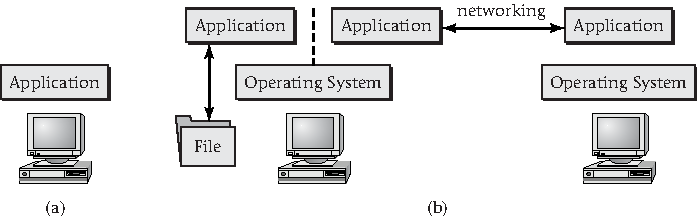
\includegraphics{hail_f0101}}
\caption{Without an operating system, a computer can directly execute
  a single program, as shown in part (a).  Part (b) shows that with an operating system,
  the computer can support concurrent computations, control the
  interactions between them (suggested by the dashed line), and allow
  communication across time and space by way of files and networking.}
\label{scan-1-1}
\end{figure}

If you have programmed only general-purpose computers, such as PCs,
workstations, and servers, you have probably never encountered a
computer system that was not running an operating system or that did
not allow multiple computations to be ongoing.  For example, when you
boot up your own computer, chances are it runs Linux, Microsoft
Windows, or Mac OS~X and that you can run multiple application
programs in individual windows on the display screen.  These three
operating systems will serve as my primary examples throughout the
book.

To illustrate that a computer can run a single program without an
operating system, consider embedded systems.  A typical
embedded system might have neither keyboard nor display screen.
Instead, it might have temperature and pressure sensors and an output
that controls the fuel injectors of your car.  Alternatively, it might have
a primitive keyboard and display, as on a microwave oven, but still
be dedicated to running a single program.

Some of the most sophisticated embedded systems run multiple
cooperating programs and use operating systems.  However, more
mundane embedded systems take a simpler form.  A single program is
directly executed by the embedded processor.  That program contains
instructions to read from input sensors, carry out appropriate
computations, and write to the output devices.  This sort of embedded
system illustrates what is possible without an operating system.  It
will also serve as a point of reference as I contrast my definition of an
operating system with an alternative definition.

One popular alternative definition of an operating system is that it
provides application programmers with an abstract view of the
underlying hardware resources, taking care of the low-level details so
that the applications can be programmed more simply.  For example, the
programmer can write a simple statement to output a string without
concern for the details of making each character appear on the display
screen.

I would counter by remarking that abstraction can be provided without
an operating system, by linking application programs with separately
written libraries of supporting procedures.  For example, a program
could output a string using the standard mechanism of a programming
language, such as C$++$ or Java.  The application programmer would not
need to know anything about hardware.  However, rather than running on an
operating system, the program could be linked together with a library
that performed the output by appropriately manipulating a microwave
oven's display panel.  Once running on the oven's embedded processor,
the library and the application code would be a single program,
nothing more than a sequence of instructions to directly execute.
However, from the application programmer's standpoint, the low-level
details would have been successfully hidden.

To summarize this argument, a library of input/output routines is not
the same as an operating system, because it satisfies only the first
part of my definition.  It does use underlying hardware to support the
execution of other software.  However, it does not provide support for
controlled interaction between computations.  In fairness to the
alternative viewpoint, it is the more historically grounded one.
Originally, a piece of software could be called an operating system
without supporting controlled interaction.  However, the language has
evolved such that my definition more closely reflects current usage.

I should also address one other alternative view of operating systems,
because it is likely to be the view you have formed from your own
experience using general-purpose computers.  You are likely to think
of an operating system as the software with which you interact in order to
carry out tasks such as running application programs.  Depending on
the user interface to which you are accustomed, you might think the
operating system is what allows you to click program icons to run
them, or you might think the operating system is what interprets
commands you type.

There is an element of truth to this perception.  The operating system
does provide the service of executing a selected application program.
However, the operating system provides this service not to human users
clicking icons or typing commands, but to other programs already
running on the computer, including the one that handles icon clicks or
command entries.  The operating system allows one program that is
running to start another program running.  This is just one of the
many services the operating system provides to running programs.
Another example service is
writing output into a file.  The sum total of features the
operating system makes available for application programmers to use in
their programs is called the \vocab{Application Programming Interface}
(\vocab{API}).  One element of the API is the ability to run other programs.

The reason why you can click a program icon or type in a command to
run a program is that general-purpose operating systems come bundled
with a user-interface program, which uses the operating system API to
run other programs in response to mouse or keyboard input.  At a
marketing level, this user-interface program may be treated as a part of
the operating system; it may not be given a prominent name of its own
and may not be available for separate purchase.

For example, Microsoft Windows comes with a user interface known as
Explorer, which provides features such as the Start menu and the
ability to click icons.  (This program is distinct from the
similarly named web browser, Internet Explorer.)  However, even if you
are an experienced Windows user, you may never have heard of Explorer;
Microsoft has chosen to give it a very low profile, treating it as an
integral part of the Microsoft Windows environment.  At a technical
level, however, it is distinct from the operating system proper.  In
order to make the distinction explicit, the true operating system is
often called the \vocab{kernel}.  The kernel is the fundamental
portion of Microsoft Windows that provides an API supporting
computations with controlled interactions.

A similar distinction between the kernel and the user interface
applies to Linux.  The Linux kernel provides the basic operating
system services through an API, whereas \vocabs{shell} are the
programs (such as bash and tcsh) that interpret typed commands, and
\vocabs{desktop environment} are the programs, such as KDE (K Desktop Environment) and GNOME,
that handle graphical interaction.

In this book, I will explain the workings of operating system
kernels, the true operating systems themselves, as opposed to the
user-interface programs.  One reason is because user-interface programs
are not constructed in any fundamentally different way than normal
application programs.  The other reason is because an operating system
need not have this sort of user interface at all.  Consider again the
case of an embedded system that controls automotive fuel
injection.  If the system is sufficiently sophisticated, it may
include an operating system.  The main control program may run other,
more specialized programs.  However, there is no ability for the user
to start an arbitrary program running through a shell or desktop
environment.  In this book, I will draw my examples from
general-purpose systems with which you might be familiar, but will emphasize
the principles that could apply in other contexts as well.

\section{What is Middleware?}\label{what-is-middleware-section}

Now that you know what an operating system is, I can turn to the other
category of software covered by this book: \vocab{middleware}.  Middleware is software occupying a middle
position between application programs and operating systems, as I will
explain in this section.

Operating
systems and middleware have much in common.  Both are software used to
support other software, such as the application programs you run.
Both provide a similar range of services centered around controlled
interaction.  Like an operating system, middleware may enforce rules
designed to keep the computations from interfering with one another.
An example is the rule that only one computation may modify a shared data structure
at a time.  Like an operating system, middleware may bring
computations at different times into contact through persistent
storage and may support interaction between computations on different
computers by providing network communication services.

Operating systems and middleware are not the same, however.  They rely upon
different underlying providers of lower-level services.  An
operating system provides the services in its API by making use of the
features supported by the hardware.  For example, it might provide API
services of reading and writing named, variable-length files by making
use of a disk drive's ability to read and write numbered, fixed-length
blocks of data.  Middleware, on the other hand, provides the services
in its API by making use of the features supported by an underlying
operating system.  For example, the middleware might provide API
services for updating relational database tables by making use of an
operating system's ability to read and write files that contain the database.

This layering of middleware on top of an operating system, as illustrated
in Figure~\ref{scan-1-2}, explains the
name; middleware is in the middle of the vertical stack, between the
application programs and the operating system.
\begin{figure}
\centerline{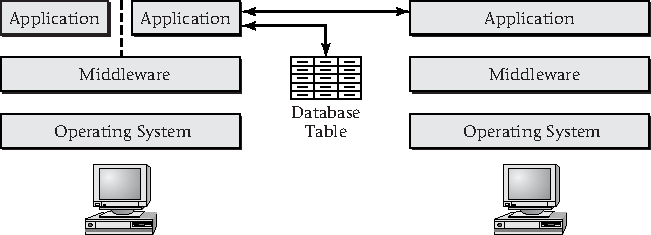
\includegraphics{hail_f0102}}
\caption{Middleware uses services from an operating system and in turn
provides services to application programs to support controlled interaction.}
\label{scan-1-2}
\end{figure}
Viewed horizontally rather than vertically, middleware is also in the
middle of interactions between different application programs
(possibly even running on different computer systems), because it
provides mechanisms to support controlled interaction through
coordination, persistent storage, naming, and communication.

I already mentioned relational database systems as one example of
middleware.  Such systems provide a more sophisticated form of persistent storage
than the files supported by most operating systems.  I use Oracle as
my primary source of examples regarding relational database systems.
Other middleware I will use for examples in the book includes the
Java~2 Platform, Enterprise Edition (J2EE) and IBM's WebSphere MQ.  These
systems provide support for keeping computations largely isolated from
undesirable interactions, while allowing them to communicate with one
another even if running on different computers.

The marketing definition of middleware doesn't always correspond
exactly with my technical definition.  In particular, some middleware
is of such fundamental importance that it is distributed as part of
the operating system bundle, rather than as a separate middleware
product.  As an example, general-purpose operating systems all come
equipped with some mechanism for translating Internet hostnames, such as
\textit{www.gustavus.edu}, into numerical addresses.  These mechanisms are
typically outside the operating system kernel, but provide a general
supporting service to application programs.  Therefore, by my
definition, they are middleware, even if not normally labeled as such.

\section{Objectives for the Book}\label{book-objectives-section}

If you work your way through this book, you will gain both knowledge
and skills.  Notice that I did not say anything about {\em reading}
the book, but rather about {\em working your way through} the book.
Each chapter in this book concludes with exercises, programming
projects, exploration projects, and some bibliographic or historical
notes.  To achieve the objectives of the book, you need to work
exercises, carry out projects, and occasionally venture down one of
the side trails pointed out by the end-of-chapter notes.  Some of the
exploration projects will specifically direct you to do research in
outside sources, such as on the Internet or in a library.  Others will
call upon you to do experimental work, such as measuring the
performance consequences of a particular design choice. If you are
going to invest that kind of time and effort, you deserve some idea of
what you stand to gain from it.  Therefore, I will explain in the
following paragraphs how you
will be more knowledgeable and skilled after finishing the book.

First, you will gain a general knowledge of how contemporary operating
systems and middleware work and some idea why they work that way.
That knowledge may be interesting in its own right, but it also has
practical applications.  Recall that these systems provide supporting
APIs for application programmers to use.  Therefore, one payoff will
be that if you program applications, you will be positioned to make
more effective use of the supporting APIs.  This is true even though
you won't be an expert at any particular API; instead, you'll see the
big picture of what services those APIs provide.

Another payoff will be if you are in a role where you need to alter
the configuration of an operating system or middleware product in order to
tune its performance or make it best serve a particular context.
Again, this one book alone won't give you all the specific knowledge
you need about any particular system, but it will give you the general
background to make sense out of more specialized references.

Perhaps the most significant payoff for learning the details
of today's systems in the context of the reasons behind their designs
is that you will be in a better position to learn tomorrow's systems.
You will be able to see in what ways they are different and in what
ways they are fundamentally still the same.  You will be able to put
new features into context, often as a new solution to an old problem,
or even just as a variant on an existing solution.  If you really get
excited by what you learn from this book, you could even use your
knowledge as the foundation for more advanced study and become one of
the people who develops tomorrow's systems.

Second, in addition to knowledge about systems, you will learn some
skills that are applicable even outside the context of operating
systems and middleware.  Some of the most important skills come from the
exploration projects.  For example, if you take those projects
seriously, you'll practice not only conducting experiments, but also
writing reports describing the experiments and their results.  That
will serve you well in many contexts.

I have also
provided you with some opportunities to develop proficiency in using the
professional literature, such as
documentation and the papers published in conference proceedings.
Those sources go into more depth than this book can, and they will
always be more up-to-date.

From the programming projects, you'll gain some skill at writing
programs that have several interacting components operating
concurrently with one another and that keep their interactions under
control.  You'll also develop some skill at writing programs that
interact over the Internet.  In neither case will you become a master
programmer.  However, in both cases, you will be laying a foundation of
skills that are relevant to a range of development projects and
environments.

Another example of a skill you can acquire is the ability to look at
the security ramifications of design decisions.  I have
a security section in each chapter, rather than a security
chapter only at the end of the book, because I want you to develop the
habit of asking, ``What are the security issues here?''  That question
is relevant even outside the realm of operating systems and
middleware.

As I hope you can see, studying operating systems and middleware can
provide a wide range of benefits, particularly if you engage yourself
in it as an active participant, rather than as a spectator.  With that
for motivation, I will now take you on another tour of the services
operating systems and middleware provide.  This tour is more detailed than
Sections \ref{what-is-os-section} and
\ref{what-is-middleware-section}, but not as detailed as Chapters
\ref{threads-chapter} through \ref{security-chapter}.

\section{Multiple Computations on One Computer}\label{concurrency-section}

The single most fundamental service an operating system provides is to
allow multiple computations to be going on at the same time, rather
than forcing each to wait until the previous one has run to
completion.  This allows desktop computers to juggle multiple tasks
for the busy humans seated in front of their screens, and it allows
server computers to be responsive to requests originating from many
different client computers on the Internet.  Beyond these
responsiveness concerns, concurrent computations can also make more
efficient use of a computer's resources.  For example, while one
computation is stalled waiting for input to arrive, another
computation can be making productive use of the processor.

A variety of words can be  used to refer to the computations underway
on a computer; they may be called threads, processes, tasks, or jobs.
In this book, I will use both the word ``thread'' and the word
``process,'' and it is important that I explain now the difference
between them.

A \vocab{thread} is the fundamental unit of concurrency.  Any one sequence of
programmed actions is a thread.  Executing a program might create
multiple threads, if the program calls for several independent
sequences of actions run concurrently with one another.  Even if each
execution of a program creates only a single thread, which is the more
normal case, a typical system will be running several threads: one for
each ongoing program execution, as well as some that are internal
parts of the operating system itself.

When you start a program running, you are always creating one or more
threads.  However, you are also creating a \vocab{process}.  The process is a
container that holds the thread or threads that you started running and
protects them from unwanted interactions with other unrelated
threads running on the same computer.  For example, a thread running
in one process cannot accidentally overwrite memory in use by a
different process.

Because human users normally start a new process running every time
they want to make a new computation happen, it is tempting to think of
processes as the unit of concurrent execution.  This temptation is
amplified by the fact that older operating systems required each
process to have exactly one thread, so that the two kinds of object
were in one-to-one correspondence, and it was not important to
distinguish them.  However, in this book, I will consistently make
the distinction.  When I am referring to the ability to set an
independent sequence of programmed actions in motion, I will write
about creating threads.  Only when I am referring to the ability to
protect threads will I write about creating processes.

In order to support threads, operating system APIs include features
such as the ability to create a new thread and to kill off an
existing thread.  Inside the operating system, there must be some
mechanism for switching the computer's attention between the various
threads.  When the operating system suspends execution of one thread
in order to give another thread a chance to make progress, the
operating system must store enough information about the first thread
to be able to successfully resume its execution later.
Chapter~\ref{threads-chapter} addresses these issues.

Some threads may not be runnable at any particular time, because they
are waiting for some event, such as the arrival of input.  However, in
general, an operating system will be confronted with multiple runnable
threads and will have to choose which ones to run at each
moment.  This problem of scheduling threads' execution has many
solutions, which are surveyed in Chapter~\ref{scheduling-chapter}.
The scheduling problem is interesting, and has generated
so many solutions, because it involves the balancing of system
users' competing interests and values.  No individual scheduling approach
will make everyone happy all the time.  My focus is on explaining how
the different scheduling approaches fit different contexts of system
usage and achieve differing goals.  In addition I explain how APIs allow
programmers to exert control over scheduling, for example, by
indicating that some threads should have higher priority than others.

\section{Controlling the Interactions Between
  Computations}\label{controlled-interaction-section}

Running multiple threads at once becomes more interesting if the
threads need to interact, rather than execute completely
independently of one another.  For example, one thread might be
producing data that another thread consumes.  If one thread is writing
data into memory and another is reading the data out, you don't want
the reader to get ahead of the writer and start reading from locations
that have yet to be written.  This illustrates one broad family of
control for interaction: control over the relative timing of the
threads' execution.  Here, a reading step must take place after the
corresponding writing step.  The general name for control over
threads' timing is \vocab{synchronization}.

Chapter~\ref{synchronization-chapter} explains several common
synchronization patterns, including keeping a consumer from
outstripping the corresponding producer.  It also explains the
mechanisms that are commonly used to provide synchronization, some of
which are supported directly by operating systems, while others
require some modest amount of middleware, such as the Java runtime
environment.

That same chapter also explains a particularly important difficulty
that can arise from the use of synchronization.  Synchronization can
force one thread to wait for another.  What if the second thread
happens to be waiting for the first?  This sort of cyclic waiting is
known as a \vocab{deadlock}.  My discussion of ways to cope with deadlock
also introduces some significant
middleware, because database systems provide an interesting example of
deadlock handling.

In Chapter~\ref{transactions-chapter}, I expand on the themes of
synchronization and middleware by explaining transactions, which are
commonly supported by middleware.  A \vocab{transaction} is a unit of
computational work for which no intermediate state from the middle of
the computation is ever visible.  Concurrent transactions are isolated
from seeing each other's intermediate storage.  Additionally, if a
transaction should fail, the storage will be left as it was before the
transaction started.
Even if the computer system should catastrophically crash in the middle of a transaction's execution, the storage after rebooting will not reflect the partial transaction.
This prevents results of a half-completed
transaction from becoming visible.  Transactions are incredibly useful
in designing reliable information systems and have widespread
commercial deployment.  They also provide a good example of how
mathematical reasoning can be used to help design practical systems;
this will be the chapter where I most prominently expect you to
understand a proof.

Even threads that have no reason to interact may accidentally
interact, if they are running on the same computer and sharing the same
memory.  For example, one thread might accidentally write into memory being used by
the other.  This is one of several reasons why operating systems
provide \foldvocab{virtual}{memory}, the topic of
Chapter~\ref{vm-chapter}.  Virtual memory refers to the technique of
modifying addresses on their way from the processor to the memory, so
that the addresses actually used for storing values in memory may be
different from those appearing in the processor's load and store
instructions.  This is a general mechanism provided through a
combination of hardware and operating system software.  I explain
several different goals this mechanism can serve, but the most
simple is isolating threads in one process from those in another by
directing their memory accesses to different regions of memory.

Having broached the topic of providing processes with isolated virtual
memory, I devote
Chapter~\ref{processes-chapter} to processes.  This chapter explains an API for
creating processes.  However, I also focus on protection
mechanisms, not only by building on Chapter~\ref{vm-chapter}'s introduction
of virtual memory, but also by explaining other forms of protection
that are
used to protect processes from one another and to protect the
operating system itself from the processes.  Some of these protection
mechanisms can be used to protect not just the storage of values in memory,
but also longer-term data storage, such as files, and even network
communication channels.  Therefore, Chapter~\ref{processes-chapter}
lays some groundwork for the later treatment of these topics.

Chapter~\ref{processes-chapter} also provides me an opportunity to
clarify one point about threads left open by
Chapter~\ref{threads-chapter}.  By showing how operating systems
provide a protective boundary between themselves and the running
application processes, I can explain where threads fall relative to
this boundary.  In particular, there are threads that are contained
entirely within the operating system kernel, others that are contained entirely
within an application process, and yet others that cross the boundary,
providing support from within the kernel for concurrent activities
within the application process.  Although it might seem natural to
discuss these categories of threads in Chapter~\ref{threads-chapter},
the chapter on threads, I really need to wait for
Chapter~\ref{processes-chapter} in order to make any more sense out of
the distinctions than I've managed in this introductory paragraph.

When two computations run concurrently on a single computer, the hard
part of supporting controlled interaction is to keep the interaction
under control.  For example, in my earlier example of a
pair of threads, one produces some data and the other consumes it.
In such a situation, there is no great mystery to how the data can flow from one to the
other, because both are using the same computer's memory.  The hard
part is regulating the use of that shared memory.  This stands in
contrast to the interactions across time and space, which I will address in Sections
\ref{persistence-section} and \ref{networking-section}.  If the producer and consumer run
at different times, or on different computers, the operating system
and middleware will need to take pains to convey the data from one to
the other.

\section{Supporting Interaction Across Time}\label{persistence-section}

General purpose operating systems all support some mechanism for
computations to leave results in long-term storage, from which they can be
retrieved by later computations.  Because this storage persists even
when the system is shut down and started back up, it is known as
\foldvocab{persistent}{storage}.  Normally, operating systems provide
persistent storage in the form of named files, which are organized into a
hierarchy of directories or folders.  Other forms of persistent
storage, such as relational database tables and application-defined
persistent objects, are generally supported by middleware.  In
Chapter~\ref{persistence-chapter}, I focus on file systems, though I
also explain some of the connections with middleware.  For example, I
compare the storage of file directories with that of database
indexes.  This comparison is particularly important as these areas are
converging.  Already the underlying mechanisms are very similar, and
file systems are starting to support indexing services like
those provided by database systems.

There are two general categories of file APIs, both of which I cover
in Chapter~\ref{persistence-chapter}.  The files can be made a part of
the process's virtual memory space, accessible with normal load and
store instructions, or they can be treated separately, as external
entities to read and write with explicit operations.

Either kind of file API provides a relatively simple interface to some
quite significant mechanisms hidden within the operating system.
Chapter~\ref{persistence-chapter} also provides a survey of some of
these mechanisms.

As an example of a simple interface to a sophisticated mechanism, an application programmer can make a file larger simply
by writing additional data to the end of the file.  The operating
system, on the other hand, has to choose the location where
the new data will be stored.  When disks are used, this space allocation has a strong
influence on performance, because of the physical realities of how
disk drives operate.

Another job for the file system is to keep track of where the data for
each file is located.  It also keeps track of other file-specific information, such as access permissions.  Thus, the file system not only
stores the files' data, but also stores \vocab{metadata},
which is data describing the data.

All these mechanisms are similar to those used by middleware for
purposes such as allocating space to hold database tables.  Operating
systems and middleware also store information,
such as file directories and database indexes, used to locate data.  The data structures
used for these naming and indexing purposes are designed for efficient
access, just like those used to track the allocation of space to
stored objects.

To make the job of operating systems and middleware even more
challenging, persistent storage structures are expected to survive
system crashes without significant loss of integrity.  For example,
it is not acceptable after a crash for specific storage space to be listed as
available for allocation and also to be listed as allocated to a file.
Such a confused state must not occur even if the crash happened just as the file was being
created or deleted.  Thus, Chapter~\ref{persistence-chapter} builds on
Chapter~\ref{transactions-chapter}'s explanation of atomic
transactions, while also outlining some other mechanisms that can be
used to protect the integrity of metadata, directories, and indexes.

Persistent storage is crucially important, perhaps even more so in the
Internet age than in prior times, because servers now hold huge
amounts of data for use by clients all over the world.  Nonetheless,
persistent storage no longer plays as unique a role as it once did.
Once upon a time, there were many computer systems in which the only
way processes communicated was through persistent storage.  Today,
that is almost unthinkable, because communication often spans the
Internet.  Therefore, as I explain in
Section~\ref{networking-section}, operating systems provide support
for networking, and middleware provides further support for the
construction of distributed systems.

\section{Supporting Interaction Across Space}\label{networking-section}

In order to build coherent software systems with components operating
on differing computers, programmers need to solve lots of problems.
Consider two examples: data flowing in a stream must be delivered in
order, even if sent by varying routes through interconnected networks,
and message delivery must be incorporated into the all-or-nothing
guarantees provided by transactions.  Luckily, application programmers
don't need to solve most of these problems, because appropriate
supporting services are provided by operating systems and middleware.

I divide my coverage of these services into two chapters.
Chapter~\ref{networking-chapter} provides a foundation regarding
networking, so that this book will stand on its own if you have not
previously studied networking.  That chapter also covers services
commonly provided by operating systems, or in close conjunction with
operating systems, such as distributed file systems.
Chapter~\ref{distmid-chapter}, in contrast, explains the higher-level
services that middleware provides for application-to-application
communication, in such forms as messaging and web services.  Each
chapter introduces example APIs that you can use as an application
programmer, as well as the more general principles behind those
specific APIs.

Networking systems, as I explain in Chapter~\ref{networking-chapter},
are generally partitioned into layers, where each layer makes use of
the services provided by the layer under it in order to provide
additional services to the layer above it.  At the bottom of the stack
is the \vocab{physical layer}, concerned with such matters as copper,
fiber optics, radio waves, voltages, and wavelengths.  Above that is
the \vocab{link layer}, which provides the service of transmitting a
chunk of data to another computer on the same local network.  This is
the point where the operating system becomes involved.  Building on
the link-layer foundation, the operating system provides the services
of the \vocab{network layer} and the \vocab{transport layer}.  The network
layer arranges for data to be relayed through interconnected networks
so as to arrive at a computer that may be elsewhere in the world.  The
transport layer builds on top of this basic computer-to-computer data
transmission to provide more useful application-to-application
communication channels.  For example, the transport layer typically
uses sequence numbering and retransmission to provide applications the
service of in-order, loss-free delivery of streams of data.  This is
the level of the most common operating system API, which provides
\vocabs{socket}, that is, endpoints for these transport-layer
connections.

The next layer up is the \vocab{application layer}.  A few specialized
application-layer services, such as distributed file systems, are
integrated with operating systems.  However, most application-layer
software, such as web browsers and email programs, is written by
application programmers.  These applications can be built directly on
an operating system's socket API and exchange streams of bytes that
comply with standardized protocols.  In
Chapter~\ref{networking-chapter}, I illustrate this possibility by
showing how web browsers and web servers communicate.

Alternatively, programmers of distributed applications can make use of
middleware to work at a higher level than sending bytes over sockets.
I show two basic approaches to this in Chapter~\ref{distmid-chapter}:
messaging and Remote Procedure Calls (RPCs).  Web services are a particular
approach to standardizing these kinds of higher-level application
communication, and have been primarily used with RPCs:
I show how to use them in this way.

In a \vocab{messaging} system, an application program requests the
delivery of a message.  The messaging system not only delivers the
message, which lower-level networking could accomplish, but also
provides additional services.  For example, the messaging is often
integrated with transaction processing.  A successful transaction may
retrieve a message from an incoming message queue, update a database in
response to that message, and send a response message to an outgoing
queue.  If the transaction fails, none of these three changes will
happen; the request message will remain in the incoming queue, the
database will remain unchanged, and the response message will not be
queued for further delivery.  Another common service provided by
messaging systems is to deliver a message to any number of recipients
who have subscribed to receive messages of a particular kind;  the
sender need not be aware of who the actual receivers are.

Middleware can also provide a mechanism for \vocab{Remote Procedure
Call} (\vocab{RPC}), in which communication between a client and a
server is made to look like an ordinary programming language procedure
call, such as invoking a method on an object.  The only difference is
that the object in question is located on a different computer, and so
the call and return involve network communication.  The middleware
hides this complexity, so that the application programmer can work
largely as though all the objects were local.  In
Chapter~\ref{distmid-chapter}, I explain this concept more fully, and then go
on to show how it plays out in the form of web services.  A \vocab{web
service} is a an application-layer entity that programs can
communicate with using standardized protocols similar to those humans
use to browse the web.

\section{Security}\label{intro-security-section}

Operating systems and middleware are often the targets of attacks by
adversaries trying to defeat system security.  Even attacks aimed at
application programs often relate to operating systems and middleware.
In particular, easily misused features of operating systems and
middleware can be the root cause of an application-level
vulnerability.  On the other hand, operating systems and middleware
provide many features that can be very helpful in constructing secure
systems.

A system is secure if it provides an acceptably low risk that an
adversary will prevent the system from achieving its owner's
objectives.  In Chapter~\ref{security-chapter}, I explain in more
detail how to think about risk and about the conflicting objectives
of system owners and adversaries.  In particular, I explain that some
of the most common objectives for owners fall into four categories:
confidentiality, integrity, availability, and accountability.  A
system provides \vocab{confidentiality} if it prevents inappropriate
disclosure of information, \vocab{integrity} if it prevents
inappropriate modification or destruction of information, and
\vocab{availability} if it prevents inappropriate interference with
legitimate usage.  A system provides \vocab{accountability} if it
provides ways to check how authorized users have exercised their
authority.  All of these rely on \vocab{authentication}, the ability
of a system to verify the identity of a user.

Many people have a narrow view of system security.  They think of
those features that would not even exist, were it not for security
issues.  Clearly, logging in with a password (or some other, better
form of authentication) is a component of system security.  Equally
clearly, having permission to read some files, but not others, is a
component of system security, as are cryptographic protocols used to
protect network communication from interception.  However, this view
of security is dangerously incomplete.

You need to keep in mind that the design of any component of the
operating system can have security consequences.  Even those parts
whose design is dominated by other considerations must also reflect
some proactive consideration of security consequences, or the overall
system will be insecure.  In fact, this is an important principle
that extends beyond the operating system to include application
software and the humans who operate it.

Therefore, I will make a habit of addressing security issues in every
chapter, rather than only at the end of the book.  Specifically, each
chapter concludes with a section pointing out some of the key security
issues associated with that chapter's topic.  I also provide a more
coherent treatment of security by concluding the book as a whole with
Chapter~\ref{security-chapter}, which is devoted exclusively to security.
That chapter takes a holistic approach to security, in which human
factors play as important a role as technical ones.

\section*{Exercises}

\begin{chapterEnumerate}
\item
What is the difference between an operating system and middleware?
\item
What do operating systems and middleware have in common?
\item
What is the relationship between threads and processes?
\item
What is one way an operating system might isolate threads from
unwanted interactions, and what is one way that middleware might do so?
\item
What is one way an operating system might provide persistent storage,
and what is one way middleware might do so?
\item
What is one way an operating system might support network
communication, and what is one way middleware might do so?
\item
Of all the topics previewed in this chapter, which one are you most
looking forward to learning more about?  Why?
\end{chapterEnumerate}

\section*{Programming Project}
\begin{chapterEnumerate}
\item
Write, test, and debug a program in the language of your choice to
carry out any task you choose.  Then write a list of all the services
you suspect the operating system is providing in order to support the
execution of your sample program.  If you think the program is also
relying on any middleware services, list those as well.
\end{chapterEnumerate}

\section*{Exploration Projects}
\begin{chapterEnumerate}
\item\label{usenix-exploration-project}
Look through the titles of the papers presented at several recent
conferences hosted by the USENIX Association (The Advanced Computing Systems Association); you can find the
conference proceedings at \textit{www.usenix.org}.  To get a better
idea what an individual paper is about, click the title to show the abstract,
which is a short summary of the paper.  Based on titles and abstracts,
pick out a few papers that you think would make interesting
supplementary reading as you work your way through this book.  Write
down a list showing the bibliographic information for the papers you
selected and, as near as you can estimate, where in this book's table
of contents they would be appropriate to read.
\item
Conduct a simple experiment in which you take some action on a
computer system and observe what the response is.  You can choose any
action you wish and any computer system for which you have
appropriate access.  You can either observe a quantitative result,
such as how long the response takes or how much output is produced, or
a qualitative result, such as in what form the response arrives.  Now, try
replicating the experiment.  Do you always get the same result?
Similar ones?  Are there any factors that need to be controlled in
order to get results that are at least approximately repeatable?  For
example, to get consistent times, do you need to reboot the system
between each trial and prevent other people from using the system? To
get consistent output, do you need to make sure input files are kept
unchanged?  If your action involves a physical device, such as a
printer, do you have to control variables such as whether the printer
is stocked with paper?  Finally, write up a careful report, in which
you explain both what experiment you tried and what results you
observed.  You should explain how repeatable the results proved to be
and what limits there were on the repeatability.  You should describe
the hardware and software configuration in enough detail that someone
else could replicate your experiment and would be likely to get
similar results.
\end{chapterEnumerate}

\section*{Notes}

The idea that an operating system should isolate computations from
unwanted interactions, and yet support desirable interactions, has a
long heritage.  A 1962 paper~\cite{max1169} by \index{Corbat{\'o}, Fernando J.}Corbat{\'o}, \index{Daggett, Marjorie Merwin}Daggett,
and \index{Daley, Robert C.}Daley points out that ``different user programs if simultaneously
in core memory may interfere with each other or the supervisor program
so some form of memory protection mode should be available when
operating user programs.'' However, that same paper goes on to say
that although ``great care went into making each user independent of
the other users \ldots\ it would be a useful extension of the system if
this were not always the case,'' so that the computer system could
support group work, such as war games.

Middleware is not as well-known to the general public as operating
systems are, though commercial information-system developers would be
lost without it.  One attempt to introduce middleware to a somewhat
broader audience was \index{Bernstein, Philip A.}Bernstein's 1996 survey article~\cite{max1016}.

The \index{USENIX}USENIX Association, mentioned in Exploration
Project~\ref{usenix-exploration-project}, is only one of several very
fine professional societies holding conferences related to the subject
matter of this book.  The reason why I specifically recommended looking through
their proceedings is that they tend to be particularly
accessible to students.  In part this is because USENIX focuses on
bringing practitioners and academics together; thus, the papers
generally are pragmatic without being superficial.
The full text is available on their web site.

%% This file is a portion of the source for Revised Edition 1.1 of
%% Operating Systems and Middleware: Supporting Controlled
%% Interaction, Copyright 2011 by Max Hailperin.  This work is
%% licensed under the Creative Commons Attribution-ShareAlike 3.0
%% Unported License. To view a copy of this license, visit
%% http://creativecommons.org/licenses/by-sa/3.0/ or send a letter to
%% Creative Commons, 171 Second Street, Suite 300, San Francisco,
%% California, 94105, USA.
\chapter{Threads}
\label{threads-chapter}
\section{Introduction}
Computer programs consist of instructions, and computers carry out
sequences of computational steps specified by those instructions.  We
call each sequence of computational steps that are strung together one after
another a \vocab{thread}.  The simplest programs to write are
single-threaded, with instructions that should be executed one after
another in a single sequence.  However, in
Section~\ref{threads-example-section}, you will learn how to write
programs that produce more than one thread of execution, each an
independent sequence of computational steps, with few if any
ordering constraints between the steps in one thread and those in
another.  Multiple threads can also come into existence by running
multiple programs, or by running the same program more than once.

Note the distinction between a program and a thread; the program
contains instructions, whereas the thread consists of the execution of
those instructions.  Even for single-threaded programs, this
distinction matters.  If a program contains a loop, then a very short
program could give rise to a very long thread of execution.  Also,
running the same program ten times will give rise to ten threads, all
executing one program.  Figure~\ref{scan-2-1} summarizes how threads
arise from programs.
\begin{figure}
\centerline{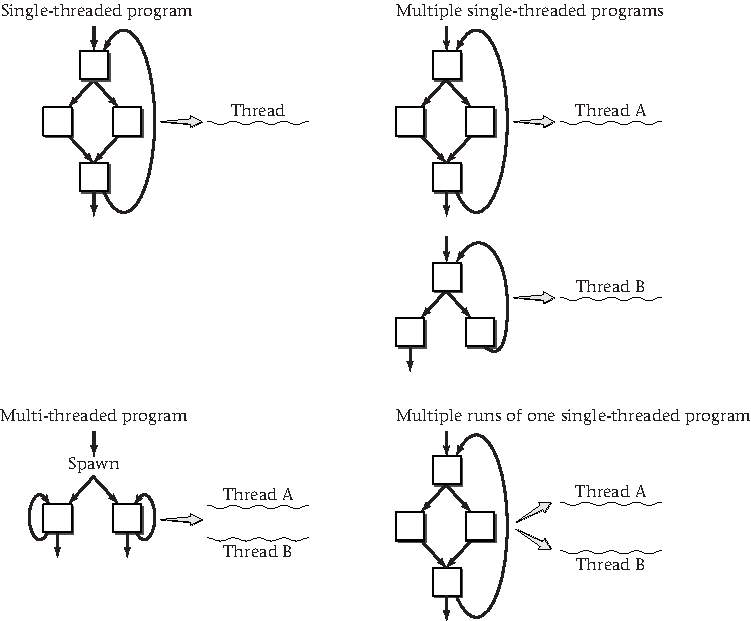
\includegraphics{hail_f0201}}
\caption{Programs give rise to threads}
\label{scan-2-1}
\end{figure}

Each thread has a lifetime, extending from the time its first
instruction execution occurs until the time of its last instruction
execution.  If two threads have overlapping lifetimes, as illustrated
in Figure~\ref{scan-2-2}, we say they are
\vocab{concurrent}.
\begin{figure}
\centerline{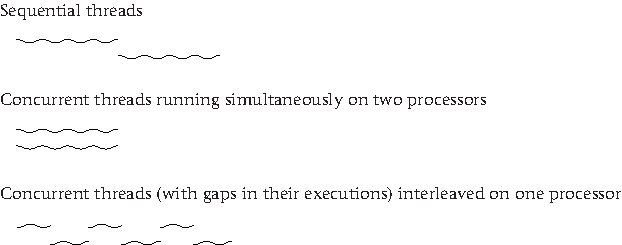
\includegraphics{hail_f0202}}
\caption{Sequential and concurrent threads}
\label{scan-2-2}
\end{figure}
One of the most fundamental goals of an operating system is to allow
multiple threads to run concurrently on the same computer.  That is,
rather than waiting until the first thread has completed before a
second thread can run, it should be possible to divide the computer's
attention between them.  If the computer hardware includes multiple
processors, then it will naturally be possible to run threads
concurrently, one per processor.  However, the operating system's
users will often want to run more concurrent threads than the hardware
has processors, for reasons described in Section~\ref{threads-uses-section}.  Therefore, the operating
system will need to divide each processor's attention between multiple
threads.  In this introductory textbook I will mostly limit myself
to the case of all the threads needing to be run on a
single processor.  I will explicitly indicate those places where I
do address the more general multi-processor case.

In order to make the concept of concurrent threads concrete,
Section~\ref{threads-example-section} shows how to write a program
that spawns multiple threads each time the program is run.  Once you
know how to create threads, I will explain in
Section~\ref{threads-uses-section} some of the reasons why it is
desirable to run multiple threads concurrently and will offer some
typical examples of the uses to which threads are put.

These first two sections explain the application programmer's view of
threads: how and why the programmer would use concurrent threads.
This sets us up for the next question: how does the operating system
support the application programmer's desire for concurrently executing
threads?  In Sections \ref{threads-switching-section} and
\ref{threads-preemptive-section}, we will examine how the system does
so.  In this chapter, we will consider only the fundamentals of how
the processor's attention is switched from one thread to another.  Some
of the related issues I address in other chapters include deciding
which thread to run at each point (Chapter~\ref{scheduling-chapter})
and controlling interaction among the threads (Chapters
\ref{synchronization-chapter}, \ref{transactions-chapter},
\ref{vm-chapter}, and \ref{processes-chapter}).
Also, as explained in Chapter~\ref{intro-chapter}, I will wait until
Chapter~\ref{processes-chapter} to explain the protection boundary
surrounding the operating system.  Thus, I will need to wait until
that chapter to distinguish threads that reside entirely within that
boundary, threads provided from inside the boundary for use outside of
it, and threads residing entirely outside the boundary (known as
\foldvocabs{user-level}{thread} or, in Microsoft Windows, \vocabs{fiber}).

Finally, the chapter concludes with the standard features of this
book: a brief discussion of security issues, followed by exercises,
programming and exploration projects, and notes.

\section{Example of Multithreaded Programs}\label{threads-example-section}

Whenever a program initially starts running, the computer carries
out the program's instructions in a single thread. Therefore, if the program is intended
to run in multiple threads, the original thread needs at some point to
spawn off a child thread that does some actions, while the parent
thread continues to do others.  (For more than two threads, the
program can repeat the thread-creation step.)  Most programming
languages have an application programming interface (or API) for
threads that includes a way to create a child thread.  In this
section, I will use
the Java API and the API for C that is called \vocabs{pthread}, for
\vocabs{POSIX thread}.  (As you will see throughout the book, POSIX is a
comprehensive specification for UNIX-like systems, including many APIs
beyond just thread creation.)

Realistic multithreaded programming requires the control of thread
interactions, using techniques I show in
Chapter~\ref{synchronization-chapter}.  Therefore, my examples in
this chapter are quite simple, just enough to show the spawning of
threads.

To demonstrate the independence of the two threads, I will have both
the parent and the child thread respond to a timer.  One will sleep
three seconds and then print out a message.  The other will sleep five
seconds and then print out a message.  Because the threads execute
concurrently, the second message will appear approximately two seconds
after the first.  (In Programming Projects
\ref{first-threads-program-input-time},
\ref{second-threads-program-input-time}, and \ref{third-threads-program-input-time},
you can write a somewhat
more realistic program, where one thread responds to user input and
the other to the timer.)

Figure~\ref{Simple2Threads} shows the Java version of this program.
The \verb|main| program first creates a
\index{Thread class@\verb"|Thread"| class}\verb|Thread| object called
\verb|childThread|.  The
\index{Runnable interface@\verb"|Runnable"| interface}\verb|Runnable| object associated
with the child thread has a \verb|run| method that sleeps three
seconds (expressed as 3000
milliseconds) and then prints a message.  This \verb|run| method starts
running when the main procedure invokes \verb|childThread.start()|.
Because the \verb|run| method is in a separate thread, the main thread
can continue on to the subsequent steps, sleeping five seconds (5000 milliseconds)
and printing its own message.
\begin{figure}
\begin{verbatim}
public class Simple2Threads {
  public static void main(String args[]){
    Thread childThread = new Thread(new Runnable(){
        public void run(){
          sleep(3000);
          System.out.println("Child is done sleeping 3 seconds.");
        }
      });
    childThread.start();
    sleep(5000);
    System.out.println("Parent is done sleeping 5 seconds.");
  }
  
  private static void sleep(int milliseconds){
    try{
      Thread.sleep(milliseconds);
    } catch(InterruptedException e){
      // ignore this exception; it won't happen anyhow
    }
  }
}
\end{verbatim}
\caption{A simple multithreaded program in Java}
\label{Simple2Threads}
\end{figure}

Figure~\ref{simple2threads} is the equivalent program in C, using the
pthreads API.  The \verb|child| procedure sleeps three seconds and prints a
message.  The \verb|main| procedure creates a \verb|child_thread|
running the \verb|child| procedure, and then itself sleeps
five seconds and prints a message.  The most significant difference from the
Java API is that
\index{pthread_create@\verb"|pthread_create"|}\verb|pthread_create|
both creates the child thread and starts it running, whereas in Java
those are two separate steps.
\begin{figure}
\begin{verbatim}
#include <pthread.h>
#include <unistd.h>
#include <stdio.h>

static void *child(void *ignored){
  sleep(3);
  printf("Child is done sleeping 3 seconds.\n");
  return NULL;
}

int main(int argc, char *argv[]){
  pthread_t child_thread;
  int code;

  code = pthread_create(&child_thread, NULL, child, NULL);
  if(code){
    fprintf(stderr, "pthread_create failed with code %d\n", code);
  }
  sleep(5);
  printf("Parent is done sleeping 5 seconds.\n");
  return 0;
}
\end{verbatim}
\caption{A simple multithreaded program in C}
\label{simple2threads}
\end{figure}

In addition to portable APIs, such as the Java and pthreads APIs, many
systems provide their own non-portable APIs.  For example, Microsoft
Windows has the Win32 API, with procedures such as \index{CreateThread@\verb"|CreateThread"|}\verb|CreateThread|
and \index{Sleep@\verb"|Sleep"|}\verb|Sleep|.  In Programming Project~\ref{win32-threads-program}, you can modify the
program from Figure~\ref{simple2threads} to use this API.

\section{Reasons for Using Concurrent Threads}\label{threads-uses-section}
You have now seen how a single execution of one program can result in
more than one thread.  Presumably, you were already at least somewhat
familiar with generating multiple threads by running multiple
programs, or by running the same program multiple times.  Regardless
of how the threads come into being, we are faced with a question.  Why
is it desirable for the computer to execute multiple threads
concurrently, rather than waiting for one to finish before starting
another?
Fundamentally, most uses for concurrent threads serve one of two goals:
\begin{description}
\item[Responsiveness:] allowing the computer system to respond quickly
  to something external to the system, such as a human user or another
  computer system.  Even if one thread is in the midst of a long
  computation, another thread can respond to the external agent.  Our
  example programs in Section~\ref{threads-example-section}
  illustrated responsiveness: both the parent and the child thread
  responded to a timer.
\item[Resource utilization:] keeping most of the hardware resources
  busy most of the time.  If one thread has no need for a
  particular piece of hardware, another may be able to make productive
  use of it.
\end{description}
Each of these two general themes has many variations, some of which we
explore in the remainder of this section.  A third reason why
programmers sometimes use concurrent threads is as a tool for
modularization.  With this, a complex system may be decomposed into a group of
interacting threads.

Let's start by considering the responsiveness of a web server, which provides many client
computers with the specific web pages they request over the Internet.
Whenever a client computer makes a network connection to the server,
it sends a sequence of bytes that contain the name of the desired web
page.  Therefore, before the server program can respond, it needs to
read in those bytes, typically using a loop that continues reading in
bytes from the network connection until it sees the end of the
request.  Suppose one of the clients is connecting using a very slow
network connection, perhaps via a dial-up modem.  The server may read
the first part of the request and then have to wait a considerable
length of time before the rest of the request arrives over the network.  What
happens to other clients in the meantime?  It would be
unacceptable for a whole web site to grind to a halt, unable to serve
any clients, just waiting for one slow client to finish issuing its
request.  One way some web servers avoid this unacceptable situation
is by using multiple threads, one for each client connection, so that
even if one thread is waiting for data from one client, other threads
can continue interacting with the other clients.
Figure~\ref{scan-2-3} illustrates the unacceptable single-threaded web
server and the more realistic multithreaded one.
\begin{figure}
\centerline{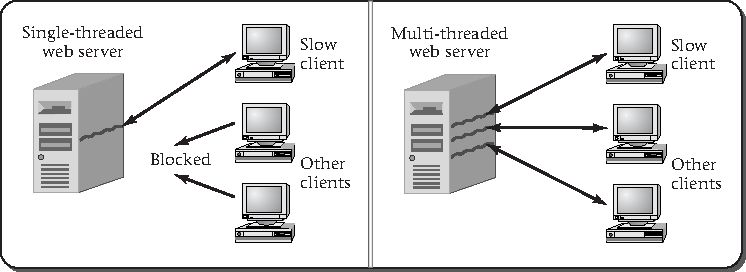
\includegraphics{hail_f0205}}
\caption{Single-threaded and multithreaded web servers}
\label{scan-2-3}
\end{figure}

On the client side, a web browser may also illustrate the need for
responsiveness.  Suppose you start loading in a very large web page,
which takes considerable time to download.  Would you be happy
if the computer froze up until the download finished?
Probably not.  You expect to be able to work on a spreadsheet in a
different window, or scroll through the first part of the web page to
read as much as has already downloaded, or at least click on the
Stop button to give up on the time-consuming download.  Each of
these can be handled by having one thread tied up loading the web page
over the network, while another thread is responsive to your actions
at the keyboard and mouse.

This web browser scenario also lets me foreshadow later portions of
the textbook concerning the controlled interaction between threads.
Note that I sketched several different things you might want
to do while the web page downloaded.  In the first case, when you work
on a spreadsheet, the two concurrent threads have almost nothing to do
with one another, and the operating system's job, beyond allowing them
to run concurrently, will mostly consist of isolating each from the
other, so that a bug in the web browser doesn't overwrite part of your
spreadsheet, for example.  This is generally done by encapsulating the
threads in separate protection environments known as \vocabes{process}, as we
will discuss in Chapters \ref{vm-chapter} and \ref{processes-chapter}.  (Some systems call processes
\vocabs{task}, while others use \vocab{task} as a synonym for \vocab{thread}.)
If, on the other hand, you continue using the browser's user interface
while the download continues, the concurrent threads are closely
related parts of a single application, and the operating system need
not isolate the threads from one another.  However, it may still need
to provide mechanisms for regulating their interaction.  For example,
some coordination between the downloading thread and the
user-interface thread is needed to ensure that you can scroll through
as much of the page as has been downloaded, but no further.  This
coordination between threads is known as \vocab{synchronization} and is
the topic of Chapters \ref{synchronization-chapter} and \ref{transactions-chapter}.

Turning to the utilization of hardware resources, the most obvious
scenario is when you have a dual-processor computer.  In this case, if
the system ran only one thread at a time, only half the processing
capacity would ever be used.  Even if the human user of the computer
system doesn't have more than one task to carry out, there may be
useful housekeeping work to keep the second processor busy.  For
example, most operating systems, if asked to allocate memory for an
application program's use, will store all zeros into the memory first.
Rather than holding up each memory allocation while the zeroing is
done, the operating system can have a thread that proactively zeros
out unused memory, so that when needed, it will be all ready.  If this
housekeeping work (zeroing of memory) were done on demand, it would
slow down the system's real work; by using a concurrent thread to
utilize the available hardware more fully, the performance is
improved.  This example also illustrates that not all threads need to
come from user programs.  A thread can be part of the operating system
itself, as in the example of the thread zeroing out unused memory.

Even in a single-processor system, resource utilization considerations
may justify using concurrent threads.  Remember that a computer
system contains hardware resources, such as
disk drives, other than the processor. Suppose you have two tasks to complete on your PC: you
want to scan all the files on disk for viruses, and you want to do a
complicated photo-realistic rendering of a three-dimensional scene
including not only solid objects, but also shadows cast on
partially transparent smoke clouds.  From experience, you know
that each of these will take about an hour.  If you do one and then
the other, it will take two hours.  If instead you do the two
concurrently---running the virus scanner in one window while you run
the graphics rendering program in another window---you may be
pleasantly surprised to find both jobs done in only an hour and a half.

The explanation for the half-hour savings in elapsed time is that the virus scanning program spends most
of its time using the disk drive to read files, with only modest
bursts of processor activity each time the disk completes a read
request, whereas the rendering program spends most of its time doing
processing, with very little disk activity.  As illustrated in Figure~\ref{scan-2-4}, running them in
sequence leaves one part of the computer's hardware idle much of the time,
whereas running the two concurrently keeps the processor and disk
drive both busy, improving the overall system efficiency.
\begin{figure}
\centerline{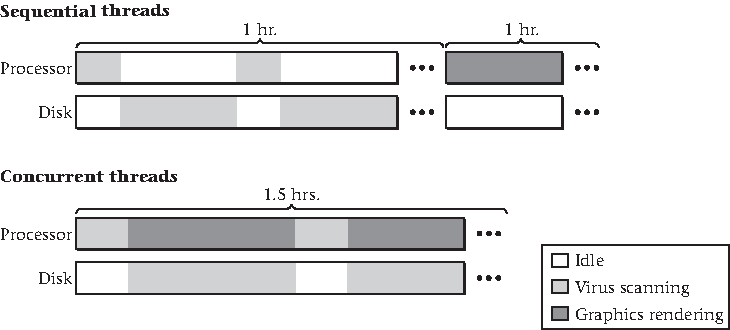
\includegraphics{hail_f0206}}
\caption{Overlapping processor-intensive and disk-intensive activities}
\label{scan-2-4}
\end{figure}
Of course,
this assumes the operating system's scheduler is smart enough to let
the virus scanner have the processor's attention (briefly) whenever a
disk request completes, rather than making it wait for the rendering
program.  I will address this issue in Chapter~\ref{scheduling-chapter}.

As you have now seen, threads can come from multiple sources and serve
multiple roles.  They can be internal portions of the operating
system, as in the example of zeroing out memory, or part of the user's
application software.  In the latter case, they can either be dividing
up the work within a multithreaded process, such as the web server
and web browser examples, or can come from multiple independent
processes, as when a web browser runs in one window and a spreadsheet
in another.  Regardless of these variations, the typical reasons
for running the threads concurrently remain unchanged: either to provide
increased responsiveness or to improve system efficiency by more fully
utilizing the hardware.  Moreover, the basic mechanism used to divide
the processor's attention among multiple threads remains the same in
these different cases as well; I describe that mechanism in Sections
\ref{threads-switching-section} and \ref{threads-preemptive-section}.
Of course, some cases require the additional protection mechanisms
provided by processes,
which we discuss in Chapters \ref{vm-chapter} and
\ref{processes-chapter}.  However, even then, it is still necessary to
leave off work on one thread and pick up work on another.

\section{Switching Between Threads}\label{threads-switching-section}

In order for the operating system to have more than one thread
underway on a processor, the system needs to have some mechanism for
switching attention between threads.  In particular, there needs to be
some way to leave off from in the middle of a thread's sequence of
instructions, work for a while on other threads, and then pick back up
in the original thread right where it left off.  In order to explain
\foldindex{thread}{switching}thread switching as simply as possible, I will initially assume that
each thread is executing code that contains, every once in a while,
explicit instructions to temporarily switch to another thread.  Once
you understand this mechanism, I can then build on it for the more
realistic case where the thread contains no explicit thread-switching
points, but rather is automatically interrupted for thread switches.

Suppose we have two threads, A and B, and we use A1, A2, A3, and so forth as
names for the instruction execution steps that constitute A, and
similarly for B.  In this case, one possible execution sequence might
be as shown in Figure~\ref{scan-2-5}.  As I will explain subsequently,
when thread A executes \verb|switchFromTo(A,B)| the computer starts
executing instructions from thread B.
\begin{figure}
\centerline{\begin{tabular}{ll}
\multicolumn{1}{c}{\underline{\textbf{thread A}}}&\multicolumn{1}{c}{\underline{\textbf{thread B}}}\\
A1&\\
A2&\\
A3&\\
\texttt{switchFromTo(A,B)}&\\
&B1\\
&B2\\
&B3\\
&\texttt{switchFromTo(B,A)}\\
A4&\\
A5&\\
\texttt{switchFromTo(A,B)}&\\
&B4\\
&B5\\
&B6\\
&B7\\
&\texttt{switchFromTo(B,A)}\\
A6&\\
A7&\\
A8&\\
\texttt{switchFromTo(A,B)}&\\
&B8\\
&B9
\end{tabular}}
\caption{Switching between threads}
\label{scan-2-5}
\end{figure}
In a more realistic example, there might be more than two threads, and
each might run for many more steps (both between switches and overall), with
only occasionally a new thread starting or an existing thread exiting.

Our goal is that the steps of each thread form a coherent execution
sequence.  That is, from the perspective of thread A, its execution
should not be much different from one in which A1 through A8 occurred
consecutively, without interruption, and similarly for thread B's
steps B1 through B9.  Suppose, for example, steps A1 and A2 load two
values from memory into registers, A3 adds them, placing the sum in a
register, and A4 doubles that register's contents, so as to get twice
the sum.  In this case, we want to make sure that A4 really does
double the sum computed by A1 through A3, rather than doubling some
other value that thread B's steps B1 through B3 happen to store in the same
register.  Thus, we can see that switching threads cannot simply be a
matter of a jump instruction transferring control to the appropriate
instruction in the other thread.  At a minimum, we will also have to
save registers into memory and restore them from there, so that when a
thread resumes execution, its own values will be back in the
registers.

In order to focus on the essentials, let's put aside the issue of how
threads start and exit.  Instead, let's focus just on the normal case where one
thread in progress puts itself on hold and switches to another thread
where that other thread last left off, such as the switch from A5 to
B4 in the preceding example.  To support switching threads,
the operating system will need to keep information about each thread,
such as at what point that thread should resume execution. If this
information is stored in a block of memory for each thread, then we
can use the addresses of those memory areas to refer to the threads.
The block of memory containing information about a thread is
called a \foldvocab{thread}{control block} or
\foldvocab{task}{control block} (\vocab{TCB}).  Thus, another way of
saying that we use the addresses of these blocks is to say that we use
pointers to thread control blocks to refer to threads.

Our fundamental thread-switching mechanism will be the
\verb|switchFromTo| procedure, which takes two of these
thread control block pointers as parameters: one specifying the
thread that is being switched out of, and one specifying the next
thread, which is being switched into.  In our running example,
\verb|A| and \verb|B| are pointer variables pointing to
the two threads' control blocks, which we use alternately in the
roles of outgoing thread and next thread.  For example, the program for
thread A contains code after instruction A5 to switch from
\verb|A| to \verb|B|, and the program for thread B
contains code after instruction B3 to switch from
\verb|B| to \verb|A|. Of course, this assumes that each
thread knows both its own identity and the identity of the thread to
switch to.  Later, we will see how this unrealistic assumption can be
eliminated.  For now, though, let's see how we could write the
\verb|switchFromTo| procedure so that
\verb|switchFromTo(A, B)| would save the current execution
status information into the structure pointed to by \verb|A|,
read back previously saved information from the structure pointed to
by \verb|B|, and resume where thread B left off.

We already saw that the execution status information to save includes
not only a position in the program, often called the \vocab{program counter}
(\vocab{PC}) or \vocab{instruction pointer} (\vocab{IP}), but also the contents of registers.
Another critical part of the execution status for programs compiled
with most higher level language compilers is a portion of the memory
used to store a stack, along with a stack pointer register that
indicates the position in memory of the current top of the stack.  You
likely have encountered this form of storage in some prior
course---computer organization, programing language principles, or
even introduction to computer science.  If not,
Appendix~\ref{stacks-appendix} provides the information you will need
before proceeding with the remainder of this chapter.

When a thread resumes execution, it must find the stack
the way it left it.  For example, suppose thread A pushes two items on the
stack and then is put on hold for a while, during which thread B executes.
When thread A resumes execution, it should find the two items it pushed at
the top of the stack---even if thread B did some pushing of its own
and has not yet gotten around to popping.  We can arrange for this by
giving each thread its own stack, setting aside a separate portion of
memory for each of them.  When thread A is executing, the \vocab{stack
pointer} (or SP register) will be pointing somewhere within thread A's
stack area, indicating how much of that area is occupied at that time.
Upon switching to thread B, we need to save away A's stack pointer,
just like other registers, and load in thread B's stack pointer.  That
way, while thread B is executing, the stack pointer will move up and
down within B's stack area, in accordance with B's own pushes and
pops.

Having discovered this need to have separate stacks and switch stack
pointers, we can simplify the saving of all other registers by
pushing them onto the stack before switching and popping them off the
stack after switching, as shown in Figure~\ref{scan-2-6}.
\begin{figure}
\centerline{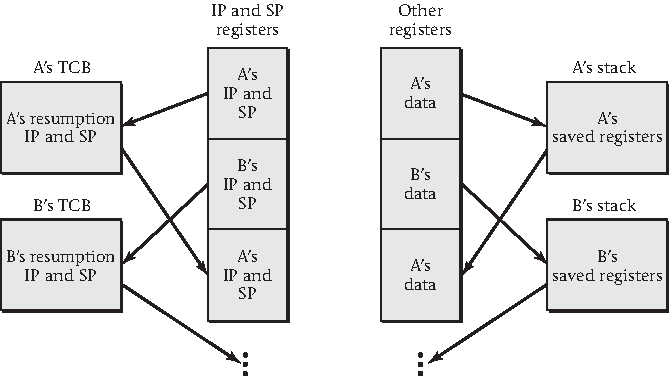
\includegraphics{hail_f0208}}
\caption{Saving registers in thread control blocks and per-thread stacks}
\label{scan-2-6}
\end{figure}
We can use this approach to outline the
code for switching from the outgoing thread to the next
thread, using \verb|outgoing| and \verb|next| as
the two pointers to thread control blocks.
(When switching from \verb|A| to \verb|B|, \verb|outgoing| will be
\verb|A| and \verb|next| will be \verb|B|.  Later, when switching back
from \verb|B| to \verb|A|, \verb|outgoing| will be \verb|B| and
\verb|next| will be \verb|A|.)
We will use
\verb|outgoing->SP| and \verb|outgoing->IP| to refer to two slots within the
structure pointed to by \verb|outgoing|, the slot used to save the stack
pointer and the one used to save the instruction pointer.  With these
assumptions, our code has the following general form:
\begin{verbatim}
  push each register on the (outgoing thread's) stack
  store the stack pointer into outgoing->SP
  load the stack pointer from next->SP
  store label L's address into outgoing->IP
  load in next->IP and jump to that address
L:
  pop each register from the (resumed outgoing thread's) stack
\end{verbatim}
Note that the code before the label (\verb|L|) is done at the time of
switching away from the outgoing thread, whereas the code after that
label is done later, upon resuming execution when some other thread
switches back to the original one.

This code not only stores the outgoing thread's stack pointer
away, but also restores the next thread's stack pointer.  Later, the
same code will be used to switch back.  Therefore, we can count on the
original thread's stack pointer to have been restored when control
jumps to label \verb|L|.  Thus, when the registers are popped, they
will be popped from the original thread's stack, matching the pushes
at the beginning of the code.

We can see how this general pattern plays out in a real system, by
looking at the thread-switching code from the Linux operating system
for the i386 architecture. (The i386 architecture is also known as the
x86 or IA-32; it is a popular processor architecture used in
standard personal computer processors such as the Pentium 4 and the
Athlon.)  If you don't want to see real code, you can skip ahead to
the paragraph after the block of assembly code.  However, even if you aren't familiar with i386 assembly language, you
ought to be able to see how this code matches the preceding pattern.

This
is real code extracted from the Linux kernel, though with some
peripheral complications left out.  The
stack pointer register is named \verb|%esp|, and when this code starts running, the
registers known as \verb|%ebx| and \verb|%esi| contain the \verb|outgoing|
and \verb|next| pointers, respectively.  Each of those pointers is the
address of a
thread control block. The location at offset 812 within the TCB contains
the thread's instruction pointer, and the location at offset 816 contains
the thread's stack pointer.  (That is, these memory locations contain
the instruction pointer and stack pointer to use when resuming that
thread's execution.)  The code surrounding the thread switch does not
keep any important values in most of the other registers; only the
special flags register and the register named \verb|%ebp| need to
be saved and restored.  With that as background, here is the
code, with explanatory comments:
%examplesource: linux-2.6.0-test1/include/asm-i386/system.h in linux-2.6.0-test1/kernel/sched.c
%exampleedit: the ret was really jmp __switch_to
\begin{verbatim}
   pushfl                 # pushes the flags on outgoing's stack
   pushl %ebp             # pushes %ebp on outgoing's stack
   movl %esp,816(%ebx)    # stores outgoing's stack pointer
   movl 816(%esi),%esp    # loads next's stack pointer
   movl $1f,812(%ebx)     # stores label 1's address,
                          #    where outgoing will resume
   pushl 812(%esi)        # pushes the instruction address
                          #    where next resumes
   ret                    # pops and jumps to that address
1: popl %ebp              # upon later resuming outgoing,
                          #    restores %ebp
   popfl                  # and restores the flags
\end{verbatim}

Having seen the core idea of how a processor is switched from running
one thread to running another, we can now eliminate the assumption
that each thread switch contains the explicit names of the outgoing
and next threads.  That is, we want to get away from having to name
threads \verb|A| and \verb|B| in
\verb|switchFromTo(A, B)|.  It is easy enough to know
which thread is being switched away from, if we just keep track at all
times of the currently running thread, for example, by storing a
pointer to its control block in a global variable called
\verb|current|.  That leaves the question of which thread is being
selected to run next.  What we will do is have the operating system
keep track of all the threads in some sort of data structure, such as
a list.  There will be a procedure, \verb|chooseNextThread()|, which
consults that data structure and, using some scheduling policy, decides
which thread to run next.  In Chapter~\ref{scheduling-chapter}, I will explain how
this scheduling is done; for now, take it as a black box.
Using this tool, one can write a procedure, \verb|yield()|, which
performs the following four steps:
\begin{verbatim}
outgoing = current;
next = chooseNextThread();
current = next;   // so the global variable will be right
switchFromTo(outgoing, next);
\end{verbatim}
Now, every
time a thread decides it wants to take a break and let other threads
run for a while, it can just invoke \verb|yield()|.
This is essentially the approach taken by real systems, such as Linux.
One complication in a \index{multiprocessor system}multiprocessor system is that the \verb|current|
thread needs to be recorded on a per-processor basis.

Thread switching is often called \foldvocab{context}{switching}, because it
switches from the execution context of one thread to that of another
thread.  Many authors, however, use the phrase \foldvocab{context}{switching} differently,
to refer to switching processes with their protection contexts---a
topic we will discuss in Chapter~\ref{processes-chapter}.  If the distinction matters,
the clearest choice is to avoid the ambiguous term
\foldvocab{context}{switching}
 and use the more specific \foldvocab{thread}{switching} or
\foldvocab{process}{switching}.

Thread switching is the most common form of
\vocab{dispatching} a thread, that is, of causing a processor to
execute it.  The only way a thread can be dispatched without a thread switch
is if a processor is idle.

\section{Preemptive Multitasking}\label{threads-preemptive-section}
At this point, I have explained thread switching well enough for
systems that employ \foldvocab{cooperative}{multitasking}, that is, where each
thread's program contains explicit code at each point where a thread
switch should occur.  However, more realistic operating systems use what
is called \foldvocab{preemptive}{multitasking}, in which the program's code
need not contain any thread switches, yet thread switches will none
the less automatically be performed from time to time.

One reason to prefer preemptive
multitasking is because it means that buggy code in one
thread cannot hold all others up.  Consider, for example, a loop that
is expected to iterate only a few times; it would seem safe, in a
cooperative multitasking system, to put thread switches only before
and after it, rather than also in the loop body.  However, a bug could
easily turn the loop into an infinite one, which would hog the
processor forever.  With preemptive multitasking, the thread may still
run forever, but at least from time to time it will be put on hold and
other threads allowed to progress.

Another reason to prefer preemptive multitasking is that it allows
thread switches to be performed when they best
achieve the goals of responsiveness and resource utilization.  For
example, the operating system can preempt a thread when input becomes
available for a waiting thread or when a hardware device falls idle.

Even with preemptive multitasking,
it may occasionally be useful for a thread to voluntarily give way to
the other threads, rather than to run as long as it is allowed.
Therefore, even preemptive systems normally provide
\verb|yield()|.
The name varies depending on the API, but often has \verb|yield| in it;
for example, the pthreads API uses the name \verb|sched_yield()|.  One
exception to this naming pattern is the Win32 API of Microsoft
Windows, which uses the name \verb|SwitchToThread()| for the equivalent
of \verb|yield()|.

Preemptive multitasking does not need any fundamentally different
thread switching mechanism; it simply needs the addition of a hardware
interrupt mechanism. In case you are not familiar with how interrupts
work, I will first take a moment to review this aspect of hardware
organization.

Normally a processor will execute consecutive instructions one after
another, deviating from sequential flow only when directed by an
explicit jump instruction or by some variant such as the \verb|ret|
instruction used in the Linux code for thread switching.
However, there is always some mechanism by which external hardware
(such as a disk drive or a network interface) can signal that it needs
attention.
A hardware timer can also be set to demand attention periodically,
such as every millisecond.
When an I/O device or timer needs attention, an \vocab{interrupt} occurs, which is almost as
though a procedure call instruction were forcibly inserted between the
currently executing instruction and the next one.  Thus, rather than
moving on to the program's next instruction, the processor jumps off
to the special procedure called the \vocab{interrupt
handler}.  The interrupt handler, which is part of the operating
system, deals with the hardware device and then executes a \vocab{return
from interrupt} instruction, which jumps back to the instruction that
had been about to execute when the interrupt occurred.  Of course, in
order for the program's execution to continue as expected, the
interrupt handler needs to be careful to save all the registers at the
start and restore them before returning.

Using this interrupt mechanism, an operating system can provide
preemptive multitasking.  When an interrupt occurs, the interrupt
handler first takes care of the immediate needs, such as
accepting data from a network interface controller or updating the
system's idea of the current time by one millisecond.  Then,
rather than simply restoring the registers and executing a return from
interrupt instruction, the interrupt handler checks whether it would
be a good time to preempt the current thread and switch to another.
For example, if the interrupt signaled the arrival of data for which a
thread had long been waiting, it might make sense to switch to
that thread.  Or, if the interrupt was from the timer and the current
thread had been executing for a long time, it may make sense to give
another thread a chance.  These policy decisions are related to
scheduling, the topic of Chapter~\ref{scheduling-chapter}.  In any case, if the
operating system decides to preempt the current thread, the interrupt
handler switches threads using a
mechanism such as the \verb|switchFromTo| procedure.

\section{Security and Threads}

One premise of this book is that every topic raises its own security
issues.  multithreading is no exception.  However, this section will
be quite brief, because with the material covered in this chapter, I can present only the
security problems connected with multithreading, not the
solutions.  So that I do not divide problems from their solutions, this
section provides only a thumbnail sketch, leaving serious
consideration of the problems and their solutions to the chapters that
introduce the necessary tools.

Security issues arise
when some threads are unable to execute because others are hogging the
computer's attention.  Security issues also arise because of unwanted
interactions between threads. Unwanted interactions include a thread writing into storage
that another thread is trying to use or reading from storage another
thread considers confidential.  These problems are most
likely to arise if the programmer has a difficult time understanding
how the threads may interact with one another.

The security section in Chapter~\ref{scheduling-chapter} addresses the
problem of some threads monopolizing the computer.  The security
sections in Chapters \ref{synchronization-chapter},
\ref{transactions-chapter}, and \ref{processes-chapter} address the
problem of controlling threads' interaction.  Each of these chapters
also has a strong emphasis on design approaches that make interactions
easy to understand, thereby minimizing the risks that arise from
incomplete understanding.

\section*{Exercises}
\begin{chapterEnumerate}
\item
Based on the examples in Section~\ref{threads-example-section},
name at least one difference between the \verb|sleep| procedure in the
POSIX API and the \verb|Thread.sleep| method in the Java API.
\item
Give at least three more examples, beyond those given in the text,
where it would be useful to run more concurrent threads on a computer
than that computer's number of processors.  Indicate how your examples
fit the general reasons to use concurrency listed in the text.
\item
Suppose thread A goes through a loop 100 times, each time performing
one disk I/O operation, taking 10~milliseconds, and then some computation, taking
1~millisecond.  While each 10-millisecond disk operation is in progress, thread A cannot
make any use of the processor.  Thread B runs for 1 second,
purely in the processor, with no I/O.  One millisecond
of processor time is spent each time the processor switches
threads; other than this switching cost, there is no problem with the
processor working on thread B during one of thread A's I/O operations.  (The
processor and disk drive do not contend for memory access bandwidth,
for example.)
\begin{enumerate}
\item
Suppose the processor and disk work purely on thread A until its
completion, and then the processor switches to thread B and runs all of
that thread.  What will the total elapsed time be?
\item
Suppose the processor starts out working on thread A, but every time
thread A performs a disk operation, the processor switches to B during
the operation and then back to A upon the disk operation's completion.
What will the total elapsed time be?
\end{enumerate}
\item
Consider a uniprocessor system where each arrival of input from an
external source triggers the creation and execution of a new thread,
which at its completion produces some output.  We are interested in
the response time from triggering input to resulting output.
\begin{enumerate}
\item
Input arrives at time 0 and again after 1~second, 2~seconds, and so forth.
Each arrival triggers a thread that takes 600~milliseconds to run.
Before the thread can run, it must be created and dispatched, which
takes 10~milliseconds.  What is the average response time for these
inputs?
\item
Now a second source of input is added, with input arriving at times
0.1~seconds, 1.1~seconds, 2.1~seconds, and so forth.  These inputs trigger
threads that only take 100~milliseconds to run, but they still need
10~milliseconds to create and dispatch.  When an input arrives, the
resulting new thread is not created or dispatched until the processor
is idle.  What is the average response time for this second class of
inputs?  What is the combined average response time for the two
classes?
\item
Suppose we change the way the second class of input is handled.  When
the input arrives, the new thread is immediately created and
dispatched, even if that preempts an already running thread.  When the
new thread completes, the preempted thread resumes execution after a
1~millisecond thread switching delay.  What is the average response
time for each class of inputs?  What is the combined average for the
two together?
\end{enumerate}
\item
When control switches away from a thread and later switches back to
that thread, the thread resumes execution where it left off.
Similarly, when a procedure calls a subroutine and later the
subroutine returns, execution picks back up where it left off in the
calling procedure.  Given this similarity, what is the essential
difference between thread switching and subroutine call/return?  You saw
that each thread has a separate stack, each in its own area of
memory.  Why is this not necessary for subroutine invocations?
\end{chapterEnumerate}

\section*{Programming Projects}
\begin{chapterEnumerate}
\item\label{first-threads-program-input-time}
If
you program in C, read the documentation for
\index{pthread_cancel@\verb"|pthread_cancel"|}\verb|pthread_cancel|. 
Using this information and the model provided in
Figure~\ref{simple2threads} on page~\pageref{simple2threads},
write a program where the initial
(main) thread creates a second thread.  The main thread should
read input from the keyboard, waiting until the user presses the Enter key.  At that point, it should kill off the
second thread and print out a message reporting that it has done so.
Meanwhile, the second thread should be in an infinite loop, each time
around sleeping five seconds and then printing out a message.  Try
running your program.  Can the sleeping thread print its periodic
messages while the main thread is waiting for keyboard input?  Can the
main thread read input, kill the sleeping thread, and print a message
while the sleeping thread is in the early part of one of its
five-second sleeps?
\item\label{second-threads-program-input-time}
If you
program in Java, read the documentation for the
\verb|stop| method in the \verb|Thread|
class.  (Ignore the information about it being deprecated.  That will
make sense only after you read Chapter~\ref{synchronization-chapter} of
this book.)  Write the program described in Programming Project~\ref{first-threads-program-input-time},
except do so in Java.  You can use the program shown in
Figure~\ref{Simple2Threads} on page~\pageref{Simple2Threads} as a model.
\item\label{third-threads-program-input-time}
Read the API documentation for some programming language other than C,
C$++$, or Java to find out how to spawn off a thread and how to
sleep.  Write a program in this language equivalent to the Java and C
example programs in Figures \ref{Simple2Threads} and
\ref{simple2threads} on pages \pageref{Simple2Threads} and
\pageref{simple2threads}.  Then do the equivalent of Programming
Projects \ref{first-threads-program-input-time} and \ref{second-threads-program-input-time} using the language you have chosen.
\item\label{win32-threads-program}
If you program in C under Microsoft Windows, you can use the
native Win32 API instead of the portable pthreads API. Read the
documentation of \verb|CreateThread| and \verb|Sleep| and modify the
program of Figure~\ref{simple2threads} on
page~\pageref{simple2threads} to use these procedures.
\end{chapterEnumerate}

\section*{Exploration Projects}
\begin{chapterEnumerate}
\item
Try the experiment of running a disk-intensive process and a
processor-intensive process concurrently.  Write a report carefully
explaining what you did and in which hardware and software system context
you did it, so that someone else could replicate your
results.  Your report should show how the elapsed time for the
concurrent execution compared with the times from sequential
execution.  Be sure to do multiple trials and to reboot the system
before each run so as to eliminate effects that come from keeping disk
data in memory for re-use.  If you can find documentation for any
performance-monitoring tools on your system, which would provide
information such as the percentage of CPU time used or the number of
disk I/O operations per second, you can include this information in
your report as well.
\item
Early versions of Microsoft Windows and Mac~OS used cooperative
multitasking.  Use the web, or other sources of information, to find
out when each switched to preemptive multitasking.  Can you find and
summarize any examples of what was written about this change at the
time?
\item
How frequently does a system switch threads?  You can find this out on
a Linux system by using the \verb|vmstat| program.  Read the
man page for \verb|vmstat|, and then run it to find the number of context
switches per second.
Write a report in which you carefully
explain what you did and the hardware and software system context in
which you did it, so that someone else could replicate your
results.
\end{chapterEnumerate}

\section*{Notes}
The idea of executing multiple threads concurrently seems to have
occurred to several people (more or less concurrently) in the late
1950s.  They did not use the word \vocab{thread}, however.  For example, a
1959 article by \index{Codd, E. F.@Codd, E.~F.}E.~F.\ Codd et al.~\cite{max984} stated that
``the second form of parallelism, which we shall call {\em nonlocal},
provides for concurrent execution of instructions which need not be
neighbors in an instruction stream, but which may belong, if you
please, to entirely separate and unrelated programs.''  From the
beginning, authors were aware of both reasons for using concurrency that I have emphasized
(resource utilization and responsiveness).  The same article by Codd
et al., for example, reports that ``one object of concurrently
running tasks which belong to different (perhaps totally unrelated)
programs is to achieve a more balanced loading of the facilities than
would be possible if all the tasks belonged to a single program.
Another object is to achieve a specified real-time response in a
situation in which messages, transactions, etc., are to be processed
on-line.''

I mentioned that an operating system may dedicate a thread to
preemptively zeroing out memory.  One example of this is the \vocab{zero
page thread} in Microsoft Windows.  See
\index{Russinovich, Mark E.}Russinovich and \index{Solomon, David A.}Solomon's
book~\cite{max981} for details.

I extracted the Linux thread switching code from version 2.6.0-test1
of the kernel.  Details (such as the offsets 812 and 816) may differ
in other versions.  The kernel source code is written in a combination
of assembly language and C, contained in
\verb|include/asm-i386/system.h| as included into
\verb|kernel/sched.c|.  To obtain pure assembly code, I fed the
source through the \verb|gcc| compiler.  Also, the \verb|ret|
instruction is a simplification; the actual kernel at that point jumps
to a block of code that ends with the \verb|ret| instruction.

My brief descriptions of the \index{POSIX}POSIX and \index{Java API}Java APIs are intended only as
concrete illustrations of broader concepts, not as a replacement for
documentation of those APIs.  You can find the official documentation
on the web at \textit{\url{http://www.unix.org}} and \textit{\url{http://java.sun.com}},
respectively.

%% This file is a portion of the source for Revised Edition 1.1 of
%% Operating Systems and Middleware: Supporting Controlled
%% Interaction, Copyright 2011 by Max Hailperin.  This work is
%% licensed under the Creative Commons Attribution-ShareAlike 3.0
%% Unported License. To view a copy of this license, visit
%% http://creativecommons.org/licenses/by-sa/3.0/ or send a letter to
%% Creative Commons, 171 Second Street, Suite 300, San Francisco,
%% California, 94105, USA.
\chapter{Scheduling}
\label{scheduling-chapter}

\section{Introduction}

In Chapter~\ref{threads-chapter} you saw that operating systems support the concurrent execution
of multiple threads by repeatedly switching each processor's attention
from one thread to another.  This switching implies that some mechanism, known
as a \vocab{scheduler}, is needed to choose which thread to run at each time.
Other system resources may need scheduling as well; for example, if
several threads read from the same disk drive, a disk
scheduler may place them in order.  For simplicity, I will consider
only processor scheduling.  Normally, when people speak of
\vocab{scheduling}, they mean processor scheduling;
similarly, the \vocab{scheduler} is understood to mean the processor
scheduler.

A scheduler should make decisions in a way that keeps the computer
system's users happy.  For example, picking the same thread all the
time and completely ignoring the others would generally not be a good
scheduling policy.  Unfortunately, there is no one policy that will
make all users happy all the time.  Sometimes the reason is as simple as
different users having conflicting desires: for example, user A wants
task A completed quickly, while user B wants task B completed quickly.
Other times, though, the relative merits of different scheduling
policies will depend not on whom you ask, but rather on the context in
which you ask.  As a simple example, a student enrolled in several
courses is unlikely to decide which assignment to work on without
considering when the assignments are due.

Because scheduling policies need to respond to context, operating
systems provide scheduling
mechanisms that leave the user in charge of more subtle policy
choices.  For example, an operating system may provide a mechanism for
running whichever thread has the highest numerical priority, while
leaving the user the job of assigning priorities to the threads.  Even
so, no one mechanism (or general family of policies) will suit all
goals.  Therefore, I spend much of this chapter describing the
different goals that users have for schedulers and the mechanisms that
can be used to achieve those goals, at least approximately.
Particularly since users may wish to achieve several conflicting
goals, they will generally have to be satisfied with ``good enough.''


\section{Thread States}\label{thread-states-section}
A typical thread will have times when it is waiting for some event,
unable to execute any useful instructions until the event occurs.
Consider a web server that reads a client's
request from the network, reads the requested web page from disk, and
then sends the page over the network to the client.  Initially the
server thread is waiting for the network interface to have some data
available.  If the server thread were scheduled on a processor while
it was waiting, the best it could do would be to execute a loop that
checked over and over whether any data has arrived---hardly a
productive use of the processor's time.  Once data is available from
the network, the server thread can execute some useful instructions to
read the bytes in and check whether the request is complete.  If not,
the server needs to go back to waiting for more data to arrive.  Once the
request is complete, the server will know what page to load from disk
and can issue the appropriate request to the disk drive.  At that
point, the thread once again needs to wait until such time as the
disk has completed the requisite physical movements to locate the
page.  To take a different example, a video display program may
display one frame of video and then wait some fraction of a second
before displaying the next so that the movie doesn't play too fast.
All the thread could do between frames would be to keep checking
the computer's real-time clock to see whether enough time had
elapsed---again, not a productive use of the processor.

In a single-thread system, it is plausible to wait by executing a loop
that continually checks for the event in question.  This approach is
known as \foldvocab{busy}{waiting}.  However, a modern general-purpose operating
system will have multiple threads competing for the processor.  In
this case, busy waiting is a bad idea because any time that the
scheduler allocates to the busy-waiting thread is lost to the other
threads without achieving any added value for the thread that is
waiting.

Therefore, operating systems provide an alternative way for threads to
wait.
The operating system keeps track of which threads can usefully run
and which are waiting.  The system does this by storing runnable threads in a
data structure called the \vocab{run queue} and waiting threads in
\vocabs{wait queue}, one per reason for waiting.  Although these
structures are conventionally called queues, they may not be used in
the first-in, first-out style of true queues.
For example, there may be a list of threads waiting for time to elapse, kept in order
of the desired time.  Another example of a wait queue would be a set of threads waiting for the
availability of data on a particular network communication channel.

Rather than executing a busy-waiting loop, a thread that wants
to wait for some event notifies the operating system of this intention.  The operating
system removes the thread from the
run queue and inserts the thread into the appropriate wait queue, as shown in
Figure~\ref{scan-3-1}.
\begin{figure}
\centerline{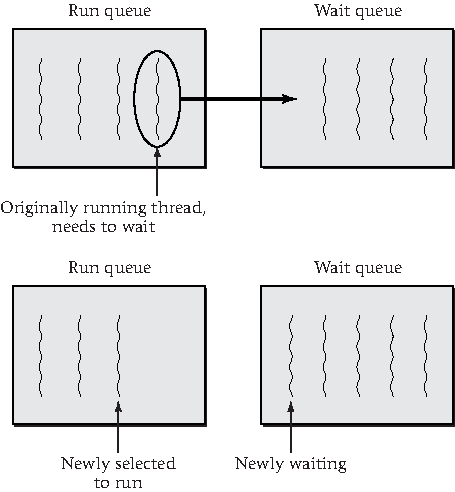
\includegraphics{hail_f0301}}
\caption{When a thread needs to wait, the operating system moves it
  from the run queue to a wait queue.  The scheduler selects one of
  the threads remaining in the run queue to dispatch, so it starts
  running.}
\label{scan-3-1}
\end{figure}
Because the
scheduler considers only threads in the run queue for execution, it
will never select
the waiting thread to run. The scheduler will be choosing only from
those threads that can make progress if given a processor on which to run.

In Chapter~\ref{threads-chapter}, I mentioned that the arrival of a hardware
interrupt can cause the processor to temporarily stop executing
instructions from the current thread and to start executing instructions
from the operating system's interrupt handler.  One of the services this
interrupt handler can perform is determining that a waiting thread doesn't
need to wait any longer.  For example, the computer's real-time clock
may be configured to interrupt the processor every one hundredth of a
second.  The interrupt handler could check the first thread in the
wait queue of threads that are waiting for specific times to elapse.  If the time
this thread was waiting for has not yet arrived, no further threads
need to be checked because the threads are kept in time order.  If,
on the other hand, the thread has slept as long as it requested, then
the operating system can move it out of the list of sleeping threads
and into the run queue, where the thread is available for scheduling.  In
this case, the operating system should check the next thread
similarly, as illustrated in Figure~\ref{scan-3-5}.
\begin{figure}
\centerline{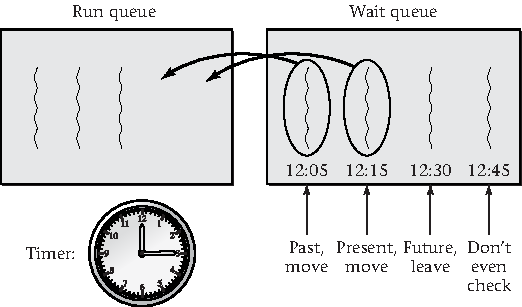
\includegraphics{hail_f0302}}
\caption{When the operating system handles a timer interrupt, all
  threads waiting for times that have now past are moved to the run
  queue. Because the wait queue is kept in time order, the scheduler
  need only check threads until it finds one waiting for a time still
  in the future. In this figure, times are shown on a human scale for
  ease of understanding.}
\label{scan-3-5}
\end{figure}

Putting together the preceding information, there are at least
three distinct states a thread can be in:
\begin{itemize}
\item \vocabindex{Runnable}{runnable} (but not running), awaiting dispatch by the scheduler
\item \vocabindex{Running}{running} on a processor
\item \vocabindex{Waiting}{waiting} for some event
\end{itemize}
Some operating systems may add a few more states in order to make
finer distinctions (waiting for one kind of event versus waiting for
another kind) or to handle special circumstances (for example, a thread that
has finished running, but needs to be kept around until another thread
is notified).  For simplicity, I will stick to the three basic states
in the foregoing list.  At critical moments in the thread's lifetime, the
operating system will change the thread's state.  These thread state
changes are indicated in Figure~\ref{state-diagram}. Again, a real
operating system may add a few additional transitions; for example, it
may be possible to forcibly terminate a thread, even while it is in a
waiting state, rather than having it terminate only of its own accord
while running.
\begin{figure}
\centerline{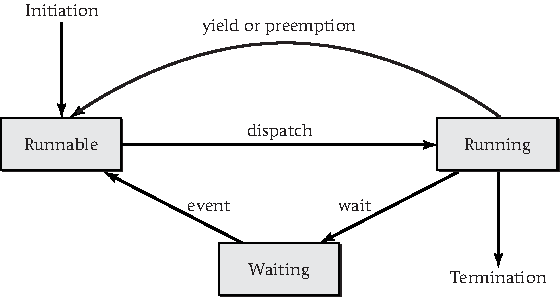
\includegraphics{hail_f0303}}
\caption{Threads change states as shown here. When a thread is initially created, it is runnable, but not
  actually running on a processor until dispatched by the scheduler.
  A running thread can voluntarily yield the processor or can be preempted
  by the scheduler in order to run another thread.  In either case,
  the formerly running thread returns to the runnable state.
  Alternatively, a running thread may wait for an external event before becoming runnable again. A running thread may also terminate.}
\label{state-diagram}
\end{figure}

\section{Scheduling Goals}\label{scheduling-goals-section}

Users expect a scheduler to maximize the computer system's
performance and to allow them to exert control.  Each of these goals
can be refined into several more precise goals, which I explain in the
following subsections.  High performance may mean high throughput
(Section~\ref{throughput-section}) or fast response time
(Section~\ref{response-time-section}), and user control may be
expressed in terms of urgency, importance, or resource allocation
(Section~\ref{uira-section}).

\subsection{Throughput}\label{throughput-section}
Many personal computers have far more processing capability available
than work to do, and they largely sit idle, patiently waiting for the next
keystroke from a user.  However, if you look behind the scenes at a large
Internet service, such as Google, you'll see a very different
situation.  Large rooms filled with rack after rack of
computers are necessary in order to keep up with the pace of incoming
requests; any one computer can cope only with a small fraction of the
traffic.  For economic reasons, the service provider wants to keep the
cluster of servers as small as possible.  Therefore, the throughput of
each server must be as high as possible.  The \vocab{throughput} is the rate
at which useful work, such as search transactions, is accomplished.
An example measure of throughput would be the number of search
transactions completed per second.

Maximizing throughput certainly implies that the scheduler should give
each processor a runnable thread on which to work, if at all possible.
However, there are some other, slightly less obvious, implications as
well.  Remember that a computer system has more components than just
processors.  It also has I/O devices (such as disk drives and network
interfaces) and a memory hierarchy, including cache memories.  Only by
using all these resources efficiently can a scheduler maximize
throughput.

I already mentioned I/O devices in Chapter~\ref{threads-chapter}, with the
example of a computationally intensive graphics rendering program
running concurrently with a disk-intensive virus scanner.  I will return
to this example later in the current chapter to see one way in which
the two threads can be efficiently interleaved.  In a nutshell, the
goal is to keep both the processor and the disk drive busy all the
time.  If you have ever had an assistant for a project, you may have some
appreciation for what this entails: whenever your assistant was in danger
of falling idle, you had to set your own work aside long enough to
explain the next assignment.  Similarly, the processor must switch
threads when necessary to give the disk more work to do.

Cache memories impact throughput-oriented scheduling in two ways,
though one arises only in \index{multiprocessor system}multiprocessor systems.  In any system,
switching between different threads more often than necessary will
reduce throughput because processor time will be wasted on the
overhead of context switching, rather than be available for useful
work.  The main source of this context-switching overhead is not the
direct cost of the switch itself, which entails saving a few registers out and
loading them with the other thread's values.  Instead, the big cost is
in reduced cache memory performance, for reasons I will explain in a
moment.  On multiprocessor systems a second issue arises:
a thread is likely to run faster when scheduled on the same
processor as it last ran on.  Again, this results from cache memory effects.  To
maximize throughput, schedulers therefore try to maintain
a specific \foldvocab{processor}{affinity} for each thread,
that is, to consistently schedule the thread on the same processor
unless there are
other countervailing considerations.

You probably learned in a computer organization course that
\vocabyies{cache memor} provide fast storage for those addresses that have been
recently accessed or that are near to recently accessed locations.
Because programs frequently access the same locations again (that is,
exhibit \foldvocab{temporal}{locality}) or access nearby locations
(that is, exhibit
\foldvocab{spatial}{locality}), the processor will often be able to get its data
from the cache rather than from the slower main memory.  Now
suppose the processor switches threads.  The new thread will have its own favorite
memory locations, which are likely to be quite different.  The cache
memory will initially suffer many misses, slowing the processor to the
speed of the main memory, as shown in Figure~\ref{scan-3-2}.
\begin{figure}
\centerline{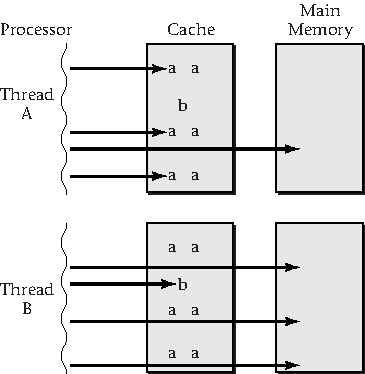
\includegraphics{hail_f0304}}
\caption{When a processor has been executing thread A for a while, the
  cache will mostly hold thread A's values, and the cache hit rate may
  be high.  If the processor then
  switches to thread B, most memory accesses will miss in the cache
  and go to the slower main memory.}
\label{scan-3-2}
\end{figure}
Over time, however, the new thread's data
will displace the data from the old thread, and the performance will
improve.  Suppose that just at the point where the cache has adapted to
the second thread, the scheduler were to decide to
switch back.  Clearly this is not a recipe for high-throughput
computing.

On a multiprocessor system, processor affinity improves throughput in
a similar manner by reducing the number of cycles the processor
stalls waiting for data from slower parts of the memory hierarchy.
Each processor has its own local cache
memory.  If a thread resumes running on the same processor on which it
previously ran, there is some hope it will find its data still in
the cache.  At worst, the thread will incur cache misses and need to
fetch the data from main memory.  The phrase ``at worst'' may seem odd
in the context of needing to go all the way to main memory, but in a
multiprocessor system, fetching from main memory is not the highest
cost situation.

Memory accesses are even more expensive if they refer
to data held in another processor's cache.  That situation can easily
arise if the thread is dispatched on a different processor than it
previously ran on, as shown in Figure~\ref{scan-3-3}
\begin{figure}
\centerline{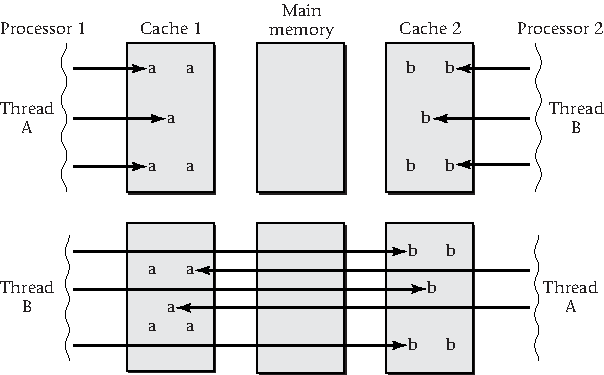
\includegraphics{hail_f0305}}
\caption{If processor 1 executes thread A and processor 2 executes
  thread B, after a while each cache will hold the corresponding
  thread's values.  If the scheduler later
  schedules each thread on the opposite processor, most
  memory accesses will miss in the local cache and need to use the
  cache coherence protocol to retrieve data from the other cache.}
\label{scan-3-3}
\end{figure}
In this circumstance, the multiprocessor system's
\foldvocab{cache}{coherence} protocol comes into play.  Typically, this means first
transferring the data from the old cache to the main memory and then
transferring it from the main memory to the new cache.  This excess
coherence traffic (beyond what is needed for blocks shared by multiple
threads) reduces throughput if the scheduler has not arranged for
processor affinity.

\subsection{Response Time}\label{response-time-section}

Other than throughput, the principle measure of a computer system's
performance is \vocab{response time}: the elapsed time from a triggering event (such as
a keystroke or a network packet's arrival) to the completed response
(such as an updated display or the transmission of a reply packet).
Notice that a high-performance system in one sense may be
low-performance in the other.  For example, frequent context switches,
which are bad for throughput, may be necessary to optimize
response time.  Systems intended for direct interaction with a single
user tend to be optimized for response time, even at the expense of
throughput, whereas centralized servers are usually designed for high
throughput as long as the response time is kept tolerable.

If an operating system is trying to schedule more than one runnable thread
per processor and if each thread is necessary in order to
respond to some event, then response time inevitably involves
tradeoffs.  Responding more quickly to one event by running the
corresponding thread means responding more slowly to some other event
by leaving its thread in the runnable state, awaiting later
dispatch.  One way to resolve this trade-off is by using
user-specified information on the relative urgency or importance of
the threads, as I describe in Section~\ref{uira-section}.  However, even without that
information, the operating system may be able to do better than just
shrug its virtual shoulders.

Consider a real world situation.  You get an email from a long-lost
friend, reporting what has transpired in her life and asking for a
corresponding update on what you have been doing for the last several
years.  You have barely started writing what will inevitably be a long
reply when a second email message arives, from a close friend, asking
whether you want to go out tonight.  You have two choices.  One is to
finish writing the long letter and then reply ``sure'' to the second
email.  The other choice is to temporarily put your long letter aside,
send off the one-word reply regarding tonight, and then go back to
telling the story of your life.  Either choice extends your response
time for one email in order to keep your response time for the other
email as short as possible.  However, that symmetry doesn't mean there is no logical
basis for choice.  Prioritizing the one-word reply provides much more
benefit to its response time than it inflicts harm on the other, more
time-consuming task.

If an operating system knows how much processor time each thread will
need in order to respond, it can use the same logic as in the email
example to guide its choices.  The policy of \vocab{Shortest Job
First} (\vocab{SJF}) scheduling minimizes the average response time,
as you can demonstrate in Exercise~\ref{Gantt-SJF-exercise}.
This policy dates back to \vocab{batch processing} systems, which processed a
single large \vocab{job} of work at a time, such as a company's
payroll or accounts payable.  System operators could minimize the
average \vocab{turnaround time} from when a job was submitted until it
was completed by processing the shortest one first.  The operators
usually had a pretty good idea how long each job would take, because
the same jobs were run on a regular basis.  However, the reason why
you should be interested in SJF is not for scheduling batch jobs
(which you are unlikely to encounter), but as background for
understanding how a modern operating system can improve the
responsiveness of threads.

Normally an operating system won't know how much processor time each
thread will need in order to respond.  One solution is to guess, based
on past behavior.  The system can prioritize those threads that have not consumed
large bursts of processor time in the past, where a \vocab{burst} is
the amount of processing done between waits for external events.
Another solution is for
the operating system to hedge its bets, so that that even if it
doesn't know which thread needs to run only briefly, it won't sink too
much time into the wrong thread.  By switching frequently between the
runnable threads, if any one of them needs only a little processing time,
it will get that time relatively soon even if the other threads
involve long computations.

The succesfulness of this hedge depends not only on the duration of
the \vocabs{time slice} given to the threads, but also on the number of runnable
threads competing for the processor.  On a lightly loaded system,
frequent switches may suffice to ensure responsiveness.  By contrast,
consider a system that is heavily loaded with many long-running
computations, but that also occasionally has an interactive thread that
needs just a little processor time.  The operating system can 
ensure responsiveness only by identifying and prioritizing the interactive
thread, so that it doesn't have to wait in line behind all the other
threads' time slices.  However brief each of those time slices is, if
there are many of them, they will add up to a substantial delay.

\subsection{Urgency, Importance, and Resource Allocation}\label{uira-section}

The goals of high throughput and quick response time do not inherently
involve user control over the scheduler; a sufficiently smart
scheduler might make all the right decisions on its own.  On the other
hand, there are user goals that revolve precisely around the desire to
be able to say the following: ``{\em This} thread is a high priority; work on it.''
I will explain three different notions that often get
confusingly lumped under the heading of priority.  To disentangle
the confusion, I will use different names for each of
them: \vocab{urgency}, \vocab{importance}, and \foldvocab{resource}{allocation}.  I will reserve
the word \vocab{priority} for my later descriptions of specific
scheduling mechanisms, where it may be used to help achieve any of the
goals: throughput, responsiveness, or the control of urgency, importance,
or resource allocation.

A task is urgent if it needs to be done soon.  For example, if you
have a small homework assignment due tomorrow and a massive term
paper to write within the next two days, the homework is more urgent.
That doesn't necessarily mean it would be smart for you to prioritize
the homework; you might make a decision to take a zero on the homework
in order to free up more time for the term paper.  If so, you are
basing your decision not only on the two tasks' urgency, but also on
their importance; the term paper is more important.  In other words,
importance indicates how much is at stake in accomplishing a task in
a timely fashion.

Importance alone is not enough to make good scheduling decisions
either.  Suppose the term paper wasn't due until a week from now.  In
that case, you might decide to work on the homework today, knowing
that you would have time to write the paper starting tomorrow.  Or, to
take a third example, suppose the term paper (which you have yet to
even start researching) was due in an hour, with absolutely no late
papers accepted.  In that case, you might realize it was hopeless to
even start the term paper, and so decide to put your time into the
homework instead.

Although urgency and importance are quite different matters, the
precision with which a user specifies urgency will determine how that
user can control scheduling to reflect importance.  If tasks have
hard deadlines, then importance can be dealt with as in the
homework example---through a process of ruthless triage.  Here,
importance measures the cost of dropping a task entirely.  On the
other hand, the deadlines may be ``soft,'' with the importance
measuring how bad it is for each task to be late.  At the other
extreme, the user might provide no information at all about urgency,
instead demanding all results ``as soon as possible.''  In this case,
a high importance task might be one to work on whenever possible,
and a low importance task might be one to fill in the idle moments,
when there is nothing more important to do.

Other than urgency and importance, another way in which users may wish to express the relationship
between different threads is by controlling what fraction of the available
processing resources they are allocated.  Sometimes, this is a matter
of fairness.  For example, if two users are sharing a computer, it
might be fair to devote half of the processing time to one user's
threads and the other half of the processing time to the other user's
threads.  In other situations, a specific degree of inequity may be
desired.  For example, a web hosting company may
sell shares of a large server to small companies for their web sites.
A company that wants to provide good service to a growing customer
base might choose to buy two shares of the web server, expecting to
get twice as much of the server's processing time in return for a
larger monthly fee.

When it was common for thousands of users, such as university
students, to share a single computer, considerable attention was
devoted to so-called \foldvocab{fair-share}{scheduling}, in which users'
consumption of the shared processor's time was balanced out over
relatively long time periods, such as a week.  That is, a user who did
a lot of computing early in the week might find his threads allocated
only a very small portion of the processor's time later in the week,
so that the other users would have a chance to catch up.
A fair share didn't have to mean an equal share; the system
administrator could grant differing allocations to different users.
For example, students taking an advanced course might receive more computing
time than introductory students.

With the advent of personal computers, fair-share scheduling has
fallen out of favor, but another resource-allocation approach,
\foldvocab{proportional-share}{scheduling}, is still very much alive. (For example,
you will see that the Linux scheduler is largely based on the
proportional-share scheduling idea.)  The main reason why I mention
fair-share scheduling is to distinguish it from proportional-share
scheduling, because the two concepts have names that are so
confusingly close.

Proportional-share scheduling balances the processing time given to
threads over a much shorter time scale, such as a second.  The idea is
to focus only on those threads that are runnable and to allocate
processor time to them in proportion with the shares the user has
specified.  For example, suppose that I have a big server on which
three companies have purchased time.  Company A pays more per month
than companies B and C, so I have given two shares to company A and
only one share each to companies B and C.  Suppose, for simplicity,
that each company runs just one thread, which I will call thread A,
B, or C, correspondingly.  If thread A waits an hour for some input to
arrive over the network while threads B and C are runnable, I will
give half the processing time to each of B and C, because they each have
one share.  When thread A's input finally arrives and the thread
becomes runnable, it won't be given an hour-long block of processing
time to ``catch up'' with the other two threads.  Instead, it will get
half the processor's time, and threads B and C will each get one
quarter, reflecting the 2:1:1 ratio of their shares.

The simplest sort of proportional-share scheduling
allows shares to be specified only for individual threads,
such as threads A, B, and C in the preceding example.
A more sophisticated version
allows shares to be specified collectively for all the threads run by
a particular user or otherwise belonging to a logical group.  For
example, each user might get an equal share of the
processor's time, independent of how many runnable threads the user
has.  Users who run multiple threads simply subdivide their shares of
the processing time.  Similarly, in the example where a big server is
contracted out to multiple companies, I would probably want to allow
each company to run multiple threads while still controlling the
overall resource allocation among the companies, not just among the
individual threads.

Linux's scheduler provides a flexible \foldvocab{group}{scheduling} facility.  Threads can be treated individually or they can be placed into groups either by user or in any other way that the system administrator chooses. Up through version 2.6.37, the default was for threads to receive processor shares individually.  However, this default changed in version 2.6.38.  The new default is to automatically establish a group for each terminal window.  That way, no matter how many CPU-intensive threads are run from within a particular terminal window, they won't greatly degrade the system's overall performance.  (To be completely precise, the automatically created groups correspond not to terminal windows, but to groupings of processes known as sessions.  Normally each terminal window corresponds to a session, but there are also other ways sessions can come into existence.  Sessions are not explained further in this book.)

Having learned about urgency, importance, and resource allocation,
one important lesson is that without further clarification, you cannot
understand what a user means by a sentence such as ``thread A is
higher priority than thread B.''  The user may want you
to devote twice as much processing time to A as to B, because A is
higher priority in the sense of meriting a larger proportion of
resources.  Then again, the user may want you to devote almost all
processing time to A, running B only in the spare moments when A goes
into a waiting state, because A is higher priority in the sense of
greater importance, greater urgency, or both.

Unfortunately, many operating systems have traditionally not given the
user a rich enough vocabulary to directly express more than one of
these goals.  For example, the UNIX family of operating systems
(including Mac OS~X and Linux) provides a way for the user to specify
the \vocab{niceness} of a thread.  The word \vocab{nice} should be understood
in the sense that a very nice thread is one that is prone to saying,
``Oh no, that's all right, you go ahead of me, I can wait.''  In other
words, a high niceness is akin to a low priority.  However, different
members of this operating system family interpret this single
parameter, niceness, differently.

The original tradition, to which Mac OS~X still adheres, is that
niceness is an expression of importance; a very nice thread should
normally only run when there is spare processor time.  Some newer
UNIX-family schedulers, such as in Linux, instead interpret the same
niceness number as an expression of resource allocation proportion,
with nicer threads getting proportionately less processor time.  It is
pointless arguing which of these interpretations of niceness is the
right one; the problem is that users have two different things they
may want to tell the scheduler, and they will never be able to do so with
only one control knob.

Luckily, some operating systems have provided somewhat more expressive
vocabularies for user control.  For example, Mac OS~X allows the user
to either express the urgency of a thread (through a deadline and
related information) or its importance (though a niceness).  These
different classes of threads are placed in a hierarchicial
relationship; the assumption is that all threads with explicit urgency
information are more important than any of the others.  Similarly, some
proportional-share schedulers, including Linux's, use niceness for
proportion control, but also allow threads to be explicitly flagged as
low-importance threads that will receive almost no processing unless a processor is otherwise idle.

As a summary of this section, Figure~\ref{scan-3-6} shows a taxonomy
of the scheduling goals I have described.  Figure~\ref{scan-3-7}
previews the scheduling mechanisms I describe in the next three
sections, and Figure~\ref{scheduling-table} shows which goals each of
them is designed to satisfy.
\begin{figure}
\centerline{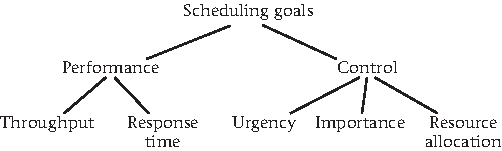
\includegraphics{hail_f0306}}
\caption{A user may want the scheduler to improve system
  performance or to allow user control.  Two different performance
  goals are high throughput and fast response time.  Three different
  ways in which a user may exert control are by specifying threads'
  urgency, importance, or resource share.}
\label{scan-3-6}
\end{figure}
\begin{figure}
\centerline{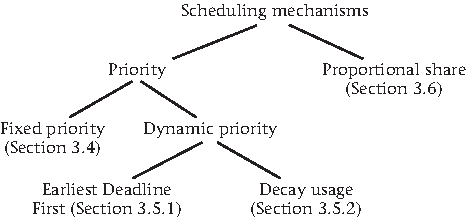
\includegraphics{hail_f0307}}
\caption{A scheduling mechanism may be based on always running the highest
  priority thread, or on pacing the threads to each receive a
  proportional share of processor time.  Priorities may be fixed, or
  they may be adjusted to reflect either the deadline by which a
  thread must finish or the thread's amount of processor usage.}
\label{scan-3-7}
\end{figure}
\begin{figure}
\centerline{\begin{tabular}{|c|c|}
\hline
\bf Mechanism & \bf Goals\\\hline
fixed priority & urgency, importance\\
Earliest Deadline First & urgency\\
decay usage & importance, throughput, response time\\
proportional share & resource allocation\\
\hline
\end{tabular}}
\caption{For each scheduling mechanism I present, I explain how it can
satisfy one or more of the scheduling goals.}
\label{scheduling-table}
\end{figure}

\section{Fixed-Priority Scheduling}\label{fixed-priority-scheduling-section}

Many schedulers use a numerical \vocab{priority} for each thread;
this controls which threads are selected for execution.  The threads with
higher priority are selected in preference to those with lower priority.
No thread will ever be running if another thread with higher priority
is not running, but is in the
runnable state.  The simplest
way the priorities can be assigned is for the user to manually specify
the priority of each thread, generally with some default value if none
is explicitly specified.  Although there may be some way for the user
to manually change a thread's priority, one speaks of \foldvocab{fixed-priority}{scheduling}
as long as the operating system never automatically adjusts a
thread's priority.

Fixed-priority scheduling suffices to achieve user goals only under limited
circumstances.  However, it is simple, so many real systems offer it, at least as one option.
For example, both Linux and Microsoft Windows allow fixed-priority
scheduling to be selected for specific threads.  Those threads take
precedence over any others, which are scheduled using other means I
discuss in Sections \ref{decay-usage-scheduling-section} and \ref{proportional-share-scheduling-section}.  In fact, fixed-priority scheduling is
included as a part of the international standard known as POSIX, which
many operating systems attempt to follow.

As an aside about priorities, whether fixed or otherwise, it is
important to note that some real systems use smaller priority numbers
to indicate more prefered threads and larger priority numbers to
indicate those that are less prefered.  Thus, a ``higher priority''
thread  may actually be indicated by a
lower priority number.
In this book, I will consistenty use ``higher priority'' and ``lower
priority'' to mean more and less prefered, independent of how those
are encoded as numbers by a particular system.

In a fixed-priority scheduler, the run queue can be kept in a
data structure ordered by priority.  If you have studied algorithms
and data structures, you know that in theory this could be efficiently
done using a clever representation of a priority queue, such as a
binary heap.  However, in practice, most operating systems use a much
simpler structure, because they use only a small range of integers for
the priorities.  Thus, it suffices to keep an array with one entry per
possible priority.  The first entry contains a list of threads with
the highest priority, the second entry contains a list of threads with
the next highest priority, and so forth.

Whenever a processor becomes idle because a thread has terminated or
entered a waiting state, the scheduler dispatches a runnable thread
of highest available priority.  The scheduler also compares priorities when a thread becomes runnable
because it is newly initiated or because it is done waiting.
If the newly runnable thread has higher priority than a running thread, the scheduler preempts the
running thread of lower priority; that is, the lower-priority thread
ceases to run and returns to the run queue.  In its
place, the scheduler dispatches the newly runnable thread of higher
priority.

Two possible strategies exist for dealing with ties, in which two or more
runnable threads have equally high priority.  (Assume there is only
one processor on which to run them, and that no thread has higher priority
than they do.)  One possibility is to run the thread
that became runnable first until it waits for some event or chooses
to voluntarily yield the processor.  Only then is the second, equally
high-priority thread dispatched. The other possibility is to share the
processor's attention between those threads that are tied for highest
priority by alternating among them in a \vocab{round-robin} fashion.  That
is, each thread runs for some small interval of time (typically tens
or hundreds of milliseconds), and then it is preempted from the clock
interrupt handler and the next thread of equal priority is dispatched,
cycling eventually back to the first of the threads.  The POSIX
standard provides for both of these options; the user can select
either a first in, first out (FIFO) policy or a round robin (RR)
policy.

Fixed-priority scheduling is not viable in an open, general-purpose
environment where a user might accidentally or otherwise create a
high-priority thread that runs for a long time.  However, in an
environment where all the threads are part of a carefully
quality-controlled system design, fixed-priority scheduling may be a
reasonable choice.  In particular, it is frequently used for so-called
\index{real-time system}\vocabs{hard-real-time system}, such as those that control the flaps on
an airplane's wings.

Threads in these hard-real-time systems normally perform periodic
tasks.  For example, one thread may wake up every second to make a
particular adjustment in the flaps and then go back to sleep for the remainder of the
second.  Each of these tasks has a deadline by which it must complete;
if the deadline is missed, the program has failed to meet its
specification.  (That is what is meant by ``hard real time.'')  In the
simplest case, the deadline is the same as the period; for example, each
second's adjustment must be done before the second is up.  The
designers of a system like this know all the threads that will be
running and carefully analyze the ensemble to make sure no deadlines
will ever be missed.  In order to do this, the designers need to have
a worst-case estimate of how long each thread will run, per period.

I can illustrate the analysis of a fixed-priority schedule for a
hard-real-time system with some simple examples, which assume
that the threads are all periodic, with deadlines equal to their
periods, and with no interactions among them other than the
competition for a single processor.  To see how the same general ideas
can be extended to cases where these assumptions don't hold, you could
read a book devoted specifically to real-time systems.

Two key theorems, proved by \index{Liu, C. L.@Liu, C.~L.}Liu and
\index{Layland, James W.}Layland in a 1973 article, make it easy
to analyze such a periodic hard-real-time system under fixed-priority
scheduling:
\begin{itemize}
\item
If the threads will meet their deadlines under any fixed priority
assignment, then they will do so under an assignment that prioritizes
threads with shorter periods over those with longer periods.
This policy is known as
\foldvocab{rate-monotonic}{scheduling}.
\item
To check that deadlines are met, it suffices to consider the worst-case situation, which is that all the threads' periods start at the
same moment.
\end{itemize}
Therefore, to test whether any fixed-priority schedule is feasible,
assign priorities in the rate-monotic fashion.  Assume all the threads
are newly runnable at time 0 and plot out what happens after
that, seeing whether any deadline is missed.

To test the feasibility of a real-time schedule, it is conventional to
use a \vocab{Gantt chart}.  This can be
used to see whether a rate-monotonic fixed-priority schedule will work
for a given set of threads.  If not, some scheduling approach other
than fixed priorities may work, or it may be necessary to redesign
using less demanding threads or hardware with more processing power.

A Gantt chart is a bar, representing the passage of time, divided into
regions labeled to show what thread is running during the
corresponding time interval.  For example, the Gantt chart
\[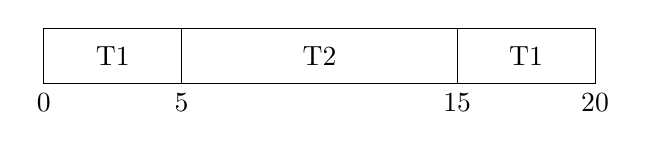
\begin{tikzpicture}[scale=.035]
\draw (0,0) rectangle (50,20);
\draw (50,0) rectangle (150,20);
\draw (150,0) rectangle (200,20);
\draw (25,10) node{T1};
\draw (100,10) node{T2};
\draw (175,10) node{T1};
\draw (0,-7) node{0};
\draw (50,-7) node{5};
\draw (150,-7) node{15};
\draw (200,-7) node{20};
\end{tikzpicture}\]
\iffalse
\[\begin{graph}(210,32)(-3,-12)
\graphlinecolour{0}
\fillednodesfalse
\rectnode{a}[50,20](25,10)
\rectnode{b}[100,20](100,10)
\rectnode{c}[50,20](175,10)
\autonodetext{a}{T1}
\autonodetext{b}{T2}
\autonodetext{c}{T1}
\freetext(0,-7){0}
\freetext(50,-7){5}
\freetext(150,-7){15}
\freetext(200,-7){20}
\end{graph}\]
\fi
\iffalse
\begin{verbatim}
+----+---------+----+
| T1 |    T2   | T1 |
+----+---------+----+
0    5         15   20
\end{verbatim}
\fi
shows thread T1 as running from time 0 to time 5 and again from time
15 to time 20; thread T2 runs from time 5 to time 15.

Consider an example with two periodically executing threads.
One, T1, has a period and deadline of four seconds and a worst-case
execution time per period of two seconds.  The other, T2, has a period
and deadline of six seconds and a worst-case execution time per
period of three seconds.  On the surface, this looks like it might
just barely be feasible on a single processor: T1 has an average
demand of half a processor (two seconds per four) and T2 also has an
average demand of half a processor (three seconds per six), totalling
to one fully utilized, but not oversubscribed, processor.  Assume
that all overheads, such as the time to do context switching between
the threads, have been accounted for by including them in the threads'
worst-case execution times.

However, to see whether this will really work without any missed
deadlines, I need to draw a Gantt chart to determine whether the threads can get the processor when
they need it.  Because T1 has the shorter
period, I assign it the higher priority.  By Liu and Layland's other
theorem, I assume both T1 and T2 are ready to start a period at time
0.  The first six seconds of the resulting Gantt chart looks like this:
\[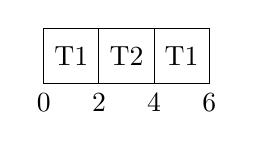
\begin{tikzpicture}[scale=.035]
\draw (0,0) rectangle (20,20);
\draw (20,0) rectangle (40,20);
\draw (40,0) rectangle (60,20);
\draw (10,10) node{T1};
\draw (30,10) node{T2};
\draw (50,10) node{T1};
\draw (0,-7) node{0};
\draw (20,-7) node{2};
\draw (40,-7) node{4};
\draw (60,-7) node{6};
\end{tikzpicture}\]
\iffalse
\[\begin{graph}(70,32)(-3,-12)
\graphlinecolour{0}
\fillednodesfalse
\rectnode{a}[20,20](10,10)
\rectnode{b}[20,20](30,10)
\rectnode{c}[20,20](50,10)
\autonodetext{a}{T1}
\autonodetext{b}{T2}
\autonodetext{c}{T1}
\freetext(0,-7){0}
\freetext(20,-7){2}
\freetext(40,-7){4}
\freetext(60,-7){6}
\end{graph}\]
\fi
\iffalse
\begin{verbatim}
+----+----+----+
| T1 | T2 | T1 |
+----+----+----+
0    2    4    6
\end{verbatim}
\fi
Note that T1 runs initially, when both threads are runnable, because
it has the higher priority.  Thus, it has no difficulty making its
deadline.  When T1 goes into a waiting state at time 2, T2 is able to
start running.  Unfortunately, it can get only two seconds of running
done by the time T1 becomes runnable again, at the start of its second
period, which is time 4.  At that moment, T2 is preempted by the
higher-priority thread T1, which occupies the processor until time 6.
Thus, T2 misses its deadline: by time 6, it has run for only two
seconds, rather than three.

If you accept Liu and Layland's theorem, you will know that switching
to the other fixed-priority assignment (with T2 higher priority than
T1) won't solve this problem.  However, rather than taking this
theorem at face value, you can draw the Gantt chart for
this alternative priority assignment in Exercise~\ref{Gantt-backward-RMS-exercise} and see that again one of the
threads misses its deadline.

In Section~\ref{dynamic-priority-scheduling-section}, I will present a scheduling mechanism
that can handle the preceding scenario successfully.
First, though, I will show one
more example---this time one for which fixed-priority scheduling
suffices.  Suppose T2's worst-case execution time were only two
seconds per six second period, with all other details the same as
before.  In this case, a Gantt chart for the first twelve seconds
would look as follows:
\[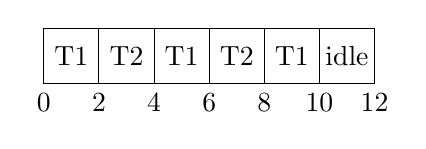
\begin{tikzpicture}[scale=.035]
\draw (0,0) rectangle (20,20);
\draw (20,0) rectangle (40,20);
\draw (40,0) rectangle (60,20);
\draw (60,0) rectangle (80,20);
\draw (80,0) rectangle (100,20);
\draw (100,0) rectangle (120,20);
\draw (10,10) node{T1};
\draw (30,10) node{T2};
\draw (50,10) node{T1};
\draw (70,10) node{T2};
\draw (90,10) node{T1};
\draw (110,10) node{idle};
\draw (0,-7) node{0};
\draw (20,-7) node{2};
\draw (40,-7) node{4};
\draw (60,-7) node{6};
\draw (80,-7) node{8};
\draw (100,-7) node{10};
\draw (120,-7) node{12};
\end{tikzpicture}\]
\iffalse
\[\begin{graph}(130,32)(-3,-12)
\graphlinecolour{0}
\fillednodesfalse
\rectnode{a}[20,20](10,10)
\rectnode{b}[20,20](30,10)
\rectnode{c}[20,20](50,10)
\rectnode{d}[20,20](70,10)
\rectnode{e}[20,20](90,10)
\rectnode{f}[20,20](110,10)
\autonodetext{a}{T1}
\autonodetext{b}{T2}
\autonodetext{c}{T1}
\autonodetext{d}{T2}
\autonodetext{e}{T1}
\autonodetext{f}{idle}
\freetext(0,-7){0}
\freetext(20,-7){2}
\freetext(40,-7){4}
\freetext(60,-7){6}
\freetext(80,-7){8}
\freetext(100,-7){10}
\freetext(120,-7){12}
\end{graph}\]
\fi
\iffalse
\begin{verbatim}
+----+----+----+----+----+----+
| T1 | T2 | T1 | T2 | T1 |idle|
+----+----+----+----+----+----+
0    2    4    6    8    10   12
\end{verbatim}
\fi
Notice that T1 has managed to execute for two seconds during each of
its three periods (0--4, 4--8, and 8--12), and that T2 has managed to
execute for two seconds during each of its two periods (0--6 and 6--12).
Thus, neither missed any deadlines.  Also, you should be able to
convince yourself that you don't need to look any further down the
timeline, because the pattern of the first 12 seconds will repeat
itself during each subsequent 12 seconds.

\section{Dynamic-Priority Scheduling}\label{dynamic-priority-scheduling-section}
Priority-based scheduling can be made more flexible by allowing the
operating system to automatically adjust threads' priorities to
reflect changing circumstances.  The relevant circumstances, and the
appropriate adjustments to make, depend what user goals the system is
trying to achieve.  In this section, I will present a couple different
variations on the theme of dynamically adjusted priorities.  First, for
continuity with Section~\ref{fixed-priority-scheduling-section},
Section~\ref{EDF-section} shows how priorities can
be dynamically adjusted for periodic hard-real-time threads using a
technique known as Earliest Deadline First scheduling.  Then
Section~\ref{decay-usage-scheduling-section} explains decay usage
scheduling, a dynamic adjustment policy commonly used in
general-purpose computing environments.

\subsection{Earliest Deadline First Scheduling}\label{EDF-section}
You saw in Section~\ref{fixed-priority-scheduling-section} that rate-monotonic scheduling is the
optimal fixed-priority scheduling method, but that even it couldn't
schedule two threads, one of which needed two seconds every four and
the other of which needed three seconds every six.  That goal is achievable
with an optimal method for dynamically assigning priorities to
threads.  This method is known as \vocab{Earliest Deadline First} (\vocab{EDF}).  In EDF scheduling,
each time a thread becomes runnable you re-assign priorities
according to the following rule: the sooner a thread's next deadline,
the higher its priority.  The optimality of EDF is another of \index{Liu, C. L.@Liu, C.~L.}Liu and
\index{Layland, James W.}Layland's theorems.

Consider again the example with T1 needing two seconds per four and T2 needing three
seconds per six.
Using EDF scheduling, the Gantt chart for the first twelve seconds of
execution would be as follows:
\[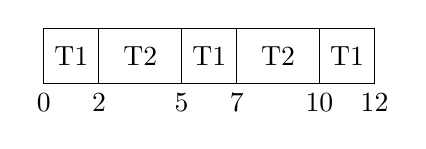
\begin{tikzpicture}[scale=.035]
\draw (0,0) rectangle (20,20);
\draw (20,0) rectangle (50,20);
\draw (50,0) rectangle (70,20);
\draw (70,0) rectangle (100,20);
\draw (100,0) rectangle (120,20);
\draw (10,10) node{T1};
\draw (35,10) node{T2};
\draw (60,10) node{T1};
\draw (85,10) node{T2};
\draw (110,10) node{T1};
\draw (0,-7) node{0};
\draw (20,-7) node{2};
\draw (50,-7) node{5};
\draw (70,-7) node{7};
\draw (100,-7) node{10};
\draw (120,-7) node{12};
\end{tikzpicture}\]
\iffalse
\[\begin{graph}(130,32)(-3,-12)
\graphlinecolour{0}
\fillednodesfalse
\rectnode{a}[20,20](10,10)
\rectnode{b}[30,20](35,10)
\rectnode{c}[20,20](60,10)
\rectnode{d}[30,20](85,10)
\rectnode{e}[20,20](110,10)
\autonodetext{a}{T1}
\autonodetext{b}{T2}
\autonodetext{c}{T1}
\autonodetext{d}{T2}
\autonodetext{e}{T1}
\freetext(0,-7){0}
\freetext(20,-7){2}
\freetext(50,-7){5}
\freetext(70,-7){7}
\freetext(100,-7){10}
\freetext(120,-7){12}
\end{graph}\]
\fi
\iffalse
\begin{verbatim}
+----+-----+----+-----+----+
| T1 | T2  | T1 | T2  | T1 |
+----+-----+----+-----+----+
0    2     5    7     10   12
\end{verbatim}
\fi
There is no need to continue the Gantt chart any further because it
will start repeating.  Notice that neither thread misses any
deadlines: T1 receives two seconds of processor time in each period
(0--4, 4--8, and 8--12), while T2 receives three seconds of processing in
each of its periods (0--6 and 6--12).  This works better
than rate-monotonic scheduling because the threads are prioritized
differently at different times.  At time 0, T1 is prioritized over T2
because its deadline is sooner (time 4 versus 6).  However, when T1
becomes runnable a second time, at time 4, it gets lower priority than
T2 because now it has a later deadline (time 8 versus 6).  Thus, the processor
finishes work on the first period of T2's work, rather than starting in
on the second period of T1's work.

In this example, there is a tie in priorities at time 8, when T1
becomes runnable for the third time.  Its deadline of 12 is the same
as T2's.  If you break the priority tie in favor of the
already-running thread, T2, you obtain the preceding Gantt chart.  In
practice, this is the correct way to break the tie, because it will result
in fewer context switches.  However, in a theoretical sense, any
tie-breaking strategy will work equally well.  In Exercise~\ref{Gantt-EDF-exercise}, you can
redraw the Gantt chart on the assumption that T2 is preempted in order
to run T1.

\subsection{Decay Usage Scheduling}\label{decay-usage-scheduling-section}
Although we all benefit from real-time control systems, such as those
keeping airplanes in which we ride from crashing, they aren't the most
prominent computers in our lives.  Instead, we mostly notice the
workstation computers that we use for daily chores, like typing this
book.  These computers may execute a few real-time threads for tasks
such as keeping an MP3 file of music decoding and playing at its
natural rate.  However, typically, most of the computer user's goals
are not expressed in terms of deadlines, but rather in terms of a
desire for quick response to interaction and efficient (high
throughput) processing of major, long-running computations.  Dynamic
priority adjustment can help with these goals too, in operating
systems such as Mac OS~X or Microsoft Windows.

Occasionally, users of general-purpose workstation computers want to
express an opinion about the priority of certain threads in order to
achieve goals related to urgency, importance, or resource allocation.
This works especially well for importance; for example, a search for
signs of extra-terrestrial intelligence might be rated a low priority
based on its small chance of success.   These
user-specified priorities can serve as \foldvocabyies{base}{priorit}, which the operating
system will use as a starting point for its automatic adjustments.
Most of the time, users will accept the default base priority for all
their threads, and so the only reason threads will differ in priority
is because of the automatic adjustments.  For simplicity, in the
subsequent discussion, I will assume that all threads have the same base
priority.

In this kind of system, threads that tie for top priority after
incorporating the automatic adjustments are processed in a
\index{round-robin}round-robin fashion, as discussed earlier.  That is, each gets to run
for one \vocab{time slice}, and then the scheduler switches
to the next of the threads.
The length of time each thread is allowed to run before switching may
also be called a \vocab{quantum}, rather than a time slice.
The thread need not run for
its full time slice; it could, for example, make an I/O request and go
into a waiting state long before the time slice is up.  In this case,
the scheduler would immediately switch to the next thread.

One reason for the operating system to adjust priorities is to
maximize throughput in a situation in which one thread is
processor-bound and another is disk-bound.  For example, in
Chapter~\ref{threads-chapter}, I introduced a scenario where the user is running a
processor-intensive graphics rendering program in one window, while
running a disk-intensive virus scanning program in another window.  As
I indicated there, the operating system can keep both the processor
and the disk busy, resulting in improved throughput relative to using
only one part of the computer system at a time.  While the disk is
working on a read request from the virus scanner, the processor can be
doing some of the graphics rendering.  As soon as the disk transaction
is complete, the scheduler should switch the processor's attention to
the virus scanner.  That way, the virus scanner can quickly look at
the data that was read in and issue its next read request, so that the
disk drive can get back to work without much delay.  The graphics
program will have time enough to run again once the virus scanning
thread is back to waiting for the disk.  In order to achieve this
high-throughput interleaving of threads, the operating system needs to
assign the disk-intensive thread a higher priority than the
processor-intensive one.

Another reason for the operating system to adjust priorities is to
minimize response time in a situation where an interactive thread is
competing with a long-running computationally intensive thread.  For
example, suppose that you are running a program in one window that is
trying to set a new world record for computing digits of $\pi$, while in
another window you are typing a term paper.  During the long pauses
while you rummage through your notes and try to think of what to write
next, you don't mind the processor giving its attention to computing
$\pi$.  But the moment you have an inspiration and start typing, you want
the word processing program to take precedence, so that it can respond
quickly to your keystrokes.  Therefore, the operating system must have
given this word processing thread a higher priority.

Notice that in both these situations, a computationally intensive
thread is competing with a thread that has been unable to use the
processor for a while, either because it was waiting for a disk
transaction to complete or because it was waiting for the user to
press another key.  Therefore, the operating system should adjust
upward the priority of threads that are in the waiting state and
adjust downward the priority of threads that are in the running state.  In a
nutshell, that is what \index{scheduling, decay usage}\vocabindex{decay usage schedulers}{decay usage scheduling}, such as the one in Mac
OS~X, do.  The scheduler in Microsoft Windows also fits the same
general pattern, although it is not strictly a  decay usage
scheduler.  I will discuss both these schedulers in more detail in the
remainder of this section.

A decay usage scheduler, such as in Mac OS~X, adjusts each thread's
priority downward from the base priority by an amount that reflects
recent processor usage by that thread.  (However, there is some cap on
this adjustment; no matter how much the thread has run, its priority
will not sink below some minimum value.)  If the thread has recently
been running a lot, it will have a priority substantially lower than
its base priority.  If the thread has not run for a long time (because
it has been waiting for the user, for example), then its priority will
equal the base priority.  That way, a thread that wakes up after a
long waiting period will take priority over a thread that has been
able to run.

The thread's recent processor usage increases when the thread runs
and \vocabs{decay} when the thread waits, as shown in
Figure~\ref{scan-3-4}.
\begin{figure}
\centerline{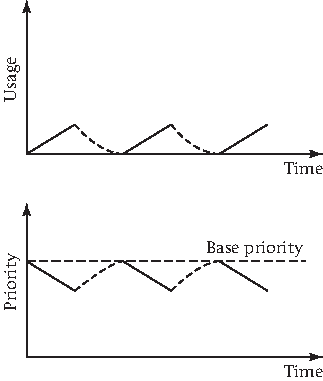
\includegraphics{hail_f0309}}
\caption{In a decay usage scheduler, such as Mac OS~X uses, a thread's
  usage increases while it runs and decays exponentially while it
  waits.  This causes the priority to decrease while running and
  increase while waiting.}
\label{scan-3-4}
\end{figure}
When the thread has been
running, its usage increases by adding in the amount of time that it
ran.  When the thread has been waiting, its usage decreases by being
multiplied by some constant every so often; for example, Mac OS~X
multiplies the usage by 5/8, eight times per second.
Rather than continuously updating the usage of every thread, the
system can calculate most of the updates to a particular thread's usage just when its state
changes, as I describe in the next two paragraphs.

The currently running thread has its usage updated whenever it voluntarily yields the
processor, has its time slice end, or faces potential preemption
because another thread comes out of the waiting state.  At these
points, the amount of time the thread has
been running is added to its usage, and its priority is correspondingly lowered.  In
Mac OS~X, the time spent in the running state is scaled by the current
overall load on the system before it is added to the thread's usage.
That way, a thread that runs during a time of high load will have its
priority drop more quickly to give the numerous other
contending threads their chances to run.

When a thread is done spending time in the waiting state, its usage is
adjusted downward to reflect the number of decay periods that have
elapsed.  For example, in Mac OS~X, the usage is multiplied by
$(5/8)^n$, where $n$ is the number of eighths of a second that have
elapsed.  Because this is an exponential decay, even a fraction of a
second of waiting is enough to bring the priority much of the way back
to the base, and after a few seconds of waiting, even a thread that
previously ran a great deal will be back to base priority.  In fact,
Mac OS~X approximates $(5/8)^n$ as 0 for $n \geq 30$, so any thread
that has been waiting for at least 3.75 seconds will be exactly at
base priority.

Microsoft Windows uses a variation on this theme.  Recall that a decay
usage scheduler adjusts the priority downward from the base to reflect
recent running and restores the priority back up toward the base
when the thead waits.  Windows does the reverse: when a thread comes
out of a wait state, it is given an elevated priority, which then
sinks back down toward the base priority as the thread runs.  The net
effect is the same: a thread that has been waiting gets a higher
priority than one that has been running.  The other difference is in
how the specific numerical size of the change is calculated.  When the
thread runs, Windows decreases its priority down to the base in a
linear fashion, as with decay usage scheduling.  However, Windows does
not use exponential decay to boost waiting threads.  Instead, a thread
that has been waiting is given a priority boost that depends on what
it was waiting for: a small boost after waiting for a disk drive, a
larger boost after waiting for input from the keyboard, and so forth.  Because
the larger boosts are associated with the kinds of waiting that
usually take longer, the net effect is broadly similar to what
exponential decay of a usage estimate achieves.

As described in Section~\ref{fixed-priority-scheduling-section}, a
scheduler can store the run queue as an array of thread lists, one per
priority level.  In this case, it can implement priority adjustments
by moving threads from one level to another.  Therefore, the Mac OS~X
and Microsoft Windows schedulers are both considered examples of the
broader class of \vocabs{multilevel feedback queue scheduler}.  The
original multilevel scheduler placed threads into levels primarily
based on the amount of main memory they used.  It also used longer
time slices for the lower priority levels.  Today, the most important
multilevel feedback queue schedulers are those approximating
decay-usage scheduling.

One advantage to decreasing the priority of running processes below
the base, as in Mac OS~X, rather than only down to the base, as in
Microsoft Windows, is that doing so will normally prevent any runnable
thread from being permanently ignored, even if a long-running thread
has a higher base priority.  Of course, a Windows partisan could reply
that if base priorities indicate importance, the less important thread
arguably should be ignored.  However, in practice, totally shutting
out any thread is a bad idea; one reason is the phenomenon of
\foldvocab{priority}{inversion}, which I will explain in Chapter~\ref{synchronization-chapter}.
Therefore, Windows has a small escape hatch: every few seconds, it
temporarily boosts the priority of any thread that is otherwise unable
to get dispatched.

One thing you may notice from the foregoing examples is the tendancy of
magic numbers to crop up in these schedulers.  Why is the usage
decayed by a factor of 5/8, eight times a second, rather than a factor
of 1/2, four times a second?  Why is the time quantum for round-robin
execution 10 milliseconds under one system and 30 milliseconds under
another?  Why does Microsoft Windows boost a thread's priority by six
after waiting for keyboard input, rather than by five or seven?

The answer to all these questions is that system designers have
tuned the numerical parameters in each system's scheduler by trial
and error.  They have done experiments using workloads similar to those
they expect their system to encounter in real use.  Keeping the
workload fixed, the experimenter varies the scheduler parameters and
measures such performance indicators as response time and throughput.
No one set of parameters will optimize all measures of performance for
all workloads.  However, by careful, systematic experimentation,
parameters can be found that are likely to keep most users happy most
of the time.  Sometimes system administrators can adjust one or more
of the parameters to suit the particular needs of their own
installations, as well.

Before leaving decay usage schedulers, it is worth pointing out one
kind of user goal that these schedulers are not very good at
achieving.  Suppose you have two processing-intensive threads and
have decided you would like to devote two-thirds of your processor's
attention to one and one-third to the other.  If other threads start
running, they can get some of the processor's time, but you still want
your first thread to get twice as much processing as any of the other
threads.  In principle, you might be able to achieve this resource
allocation goal under a decay usage scheduler by appropriately
fiddling with the base priorities of the threads.  However, in
practice it is very difficult to come up with appropriate base
priorities to achieve desired processor proportions.  Therefore, if
this kind of goal is important to a system's users, a different form
of scheduler should be used, such as I discuss in Section~\ref{proportional-share-scheduling-section}.

\section{Proportional-Share Scheduling}\label{proportional-share-scheduling-section}
\foldindex{proportional-share}{scheduling}
When resource allocation is a primary user goal, the scheduler needs
to take a somewhat longer-term perspective than the approaches I have
discussed thus far.  Rather than focusing just on which thread is most
important to run at the moment, the scheduler needs to be pacing the
threads, doling out processor time to them at controlled rates.

Researchers have proposed three basic mechanisms for controlling the
rate at which threads are granted processor time:
\begin{itemize}
\item
Each thread can be granted the use of the processor equally often,
just as in a simple round-robin. However, those that have larger
allocations are granted a longer time slice each time around than
those with smaller allocations.  This mechanism is known as \foldvocab{weighted round-robin}{scheduling} (\vocab{WRR}).
\item
A uniform time slice can be used for all threads.  However, those that
have larger allocations can run more often, because the threads with
smaller allocations ``sit out'' some of the rotations through the list
of runnable threads.  Several names are used for this mechanism, depending
on the context and minor variations: \vocab{weighted fair queuing} (\vocab{WFQ}),
\foldvocab{stride}{scheduling}, and \foldvocab{virtual time round-robin}{scheduling} (\vocab{VTRR}).
\item
A uniform time slice can be used for all threads.  However, those with
larger allocations are chosen to run more often (on the average),
because the threads are selected by a lottery with weighted odds,
rather than in any sort of rotation.  This mechanism is called \foldvocab{lottery}{scheduling}.
\end{itemize}

Lottery scheduling is not
terribly practical, because although each thread will get its
appropriate share of processing time over the long run, there may be
significant deviations over the short run. Consider, for example, a
system with two threads, each of which should get half the processing
time.  If the time-slice duration is one twentieth of a second, each
thread should run ten times per second.  Yet one thread might get shut
out for a whole second, risking a major loss of responsiveness, just
by having a string of bad luck.  A coin flipped twenty times per
second all day long may well come up heads twenty times in a row at
some point.  In Programming Project~\ref{Bernoulli-run-project}, you
will calculate the probability and discover that over the course of a
day the chance of one thread or the other going a whole second
without running is actually quite high.
Despite this shortcoming,
lottery scheduling
has received considerable attention in the research
literature.

Turning to the two non-lottery approaches, I can
illustrate the difference between them with an example.  Suppose
three threads (T1, T2, and T3) are to be allocated
resources in the proportions 3:2:1.  Thus, T1 should get half the
processor's time, T2 one-third, and T3 one-sixth.  With
weighted round-robin scheduling, I might
get the following Gantt chart with times in milliseconds:
\[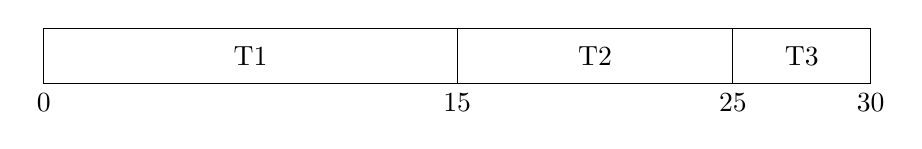
\begin{tikzpicture}[scale=.035]
\draw (0,0) rectangle (150,20);
\draw (150,0) rectangle (250,20);
\draw (250,0) rectangle (300,20);
\draw (75,10) node{T1};
\draw (200,10) node{T2};
\draw (275,10) node{T3};
\draw (0,-7) node{0};
\draw (150,-7) node{15};
\draw (250,-7) node{25};
\draw (300,-7) node{30};
\end{tikzpicture}\]
\iffalse
\[\begin{graph}(310,32)(-3,-12)
\graphlinecolour{0}
\fillednodesfalse
\rectnode{a}[150,20](75,10)
\rectnode{b}[100,20](200,10)
\rectnode{c}[50,20](275,10)
\autonodetext{a}{T1}
\autonodetext{b}{T2}
\autonodetext{c}{T3}
\freetext(0,-7){0}
\freetext(150,-7){150}
\freetext(250,-7){250}
\freetext(300,-7){300}
\end{graph}\]
\fi
Taking the other approach, I could use a fixed time slice of
5~milliseconds, but with T2 sitting out one round in every three, and
T3 sitting out two rounds out of three.  The Gantt chart for the first
three scheduling rounds would look as follows (thereafter, the pattern
would repeat):
\[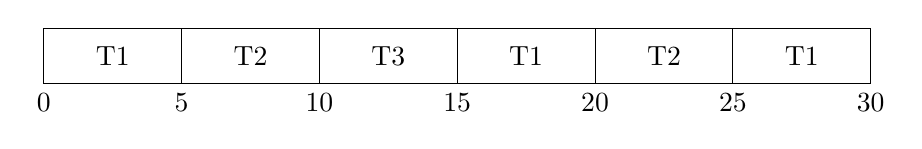
\begin{tikzpicture}[scale=.035]
\draw (0,0) rectangle (50,20);
\draw (50,0) rectangle (100,20);
\draw (100,0) rectangle (150,20);
\draw (150,0) rectangle (200,20);
\draw (200,0) rectangle (250,20);
\draw (250,0) rectangle (300,20);
\draw (25,10) node{T1};
\draw (75,10) node{T2};
\draw (125,10) node{T3};
\draw (175,10) node{T1};
\draw (225,10) node{T2};
\draw (275,10) node{T1};
\draw (0,-7) node{0};
\draw (50,-7) node{5};
\draw (100,-7) node{10};
\draw (150,-7) node{15};
\draw (200,-7) node{20};
\draw (250,-7) node{25};
\draw (300,-7) node{30};
\end{tikzpicture}\]
\iffalse
\[\begin{graph}(310,32)(-3,-12)
\graphlinecolour{0}
\fillednodesfalse
\rectnode{a}[50,20](25,10)
\rectnode{b}[50,20](75,10)
\rectnode{c}[50,20](125,10)
\rectnode{d}[50,20](175,10)
\rectnode{e}[50,20](225,10)
\rectnode{f}[50,20](275,10)
\autonodetext{a}{T1}
\autonodetext{b}{T2}
\autonodetext{c}{T3}
\autonodetext{d}{T1}
\autonodetext{e}{T2}
\autonodetext{f}{T1}
\freetext(0,-7){0}
\freetext(50,-7){50}
\freetext(100,-7){100}
\freetext(150,-7){150}
\freetext(200,-7){200}
\freetext(250,-7){250}
\freetext(300,-7){300}
\end{graph}\]
\fi

Weighted round-robin scheduling has the advantage of fewer thread switches.  Weighted fair queueing, on the other hand, can keep the threads accumulated runtimes more consistently close to the desired proportions.  Exercise~\ref{WRR-WFQ-comparison-exercise} allows you to explore the difference.

In
Linux, the user-specified \vocab{niceness} of a thread controls the
proportion of processor time that the thread will receive.
The core of the scheduling algorithm is a weighted round-robin, as in the first
Gantt chart.
(A separate scheduling policy is used for
fixed-priority scheduling
of real-time threads.  The discussion
here concerns the scheduler  used for
ordinary threads.)
This proportional-share scheduler is called the \vocab{Completely Fair Scheduler} (\vocab{CFS}).
On a multiprocessor system, CFS schedules the threads running on each processor; a largely independent
mechanism balances the overall computational load between processors.  The end-of-chapter notes
revisit the question of how proportional-share scheduling fits into the multiprocessor context.

Rather than directly assign each niceness level a time slice, CFS assigns
each niceness level a \textit{weight} and then calculates the time slices
based on the weights of the runnable threads.  Each thread is given a
time slice proportional to its weight divided by the total weight of
the runnable threads.  CFS starts with a target time for how long it
should take to make one complete round-robin through the runnable
threads.  Suppose, for example, that the target is 6~milliseconds.  Then with
two runnable threads of equal niceness, and hence equal weight, each
thread will run for 3~milliseconds, independent of whether they both have
niceness 0 or both have niceness 19.  With four equal-niceness
threads, each would run 1.5~milliseconds.

Notice that the thread-switching rate is dependent on the overall
system load, unlike with a fixed time slice.  This means that as a
system using CFS becomes more loaded, it will tend to sacrifice some
throughput in order to retain a desired level of responsiveness.  The
level of responsiveness is controlled by the target time that a thread
may wait between successive opportunities to run, which  is settable by the system
administrator.  The value of 6~milliseconds used in the examples is the
default for uniprocessor systems.

However, if system load becomes extremely high, CFS does not
continue sacrificing throughput to response time.  This is because
there is a lower bound on how little time each thread can receive.
After that point is reached, adding additional threads will increase
the total time to cycle through the threads, rather than continuing to
reduce the per-thread time.  The minimum time per thread is also a
parameter the system administrator can configure; the default value
causes the time per thread to stop shrinking once the number of runnable threads reaches 8.

Now consider a case where two threads share the CPU, one with
niceness 0 and the other with niceness 5.  CFS assigns these niceness
levels the weights of 1024 and 335 respectively.  The time that the
threads get is therefore proportional to $1024/(1024+335)$ and
$335/(1024+335)$.  Because 1024 is roughly 3 times as large as 335, we
can estimate that the thread with niceness 0 will receive
approximately 4.5~milliseconds out of each 6~milliseconds and
the thread with niceness 5 will receive approximately 1.5~milliseconds out of each
6~milliseconds.  The same result would be achieved if
the threads had niceness 5 and 10 rather than 0 and 5, because the
weights would then be 335 and 110, which are still in approximately a
3-to-1 ratio.  More generally, the CPU proportion is determined only
by the relative difference in nicenesses, rather than the absolute
niceness levels, because the weights are arranged in a geometric
progression.  (This is analogous to well-tempered musical scales, where a particular
interval, such as a major fifth, has the same harmonic quality no
matter where on the scale it is positioned, because the ratio of
frequencies is the same.)

Having seen this overview of how nicenesses control the allocation of
processor time in CFS, we can now move into a discussion of the actual
mechanism used to meter out the processor time.
The CFS scheduling mechanism is based around one big idea, with
lots of smaller details that I will largely ignore.

The big idea is
keeping track for each thread of how much total running it has done,
measured in units that are scaled in accordance with the thread's
weight.  That is, a niceness 0 thread is credited with 1~nanosecond of running
for each nanosecond of time that elapses with the thread running, but
a niceness 5 thread would be credited with approximately 3~nanoseconds of
running for each nanosecond it actually runs.  (More precisely, it
would be credited with 1024/335 nanoseconds of running for each
actual nanosecond.)

Given this funny accounting of how much running
the threads are doing (which is called \foldvocab{virtual}{runtime}), the goal of keeping the threads running in
their proper proportion simply amounts to running whichever is the
furthest behind.  However, if CFS always devoted the CPU to the thread that was furthest behind,
it would be constantly switching back and forth between the threads.
Instead, the scheduler sticks with the current thread until its
time slice runs out or it is preempted by a waking thread.
Once the scheduler does choose a new thread, it picks the thread
with minimum virtual runtime.  Thus, over the long haul, the virtual
runtimes are kept approximately in balance, which means the actual
runtimes are kept in the proportion specified by the threads'
weights, which reflect the threads'
nicenesses.

This concept of keeping virtual runtimes in balance is important enough
to consider a couple concrete examples.
First, consider a case where two threads have equal niceness, so the scheduler tries to make
sure that the two threads have run for equal amounts of time. After $x$
nanoseconds have elapsed, each of the two threads should have run for $x/2$
nanoseconds.  To make this always exactly true, the scheduler would need to
keep switching back and for between the threads, which is inefficient.  Instead, the scheduler is willing to stick with one thread for a length of
time, the time slice.  As a result, you might see that after 9~milliseconds,
instead of each of the two threads having run for 4.5~milliseconds, maybe
Thread~A has run for 6~milliseconds and Thread~B has run for 3~milliseconds,
as shown in Figure~\ref{equal-virtual-runtime-figure}.  When the scheduler decides which thread to run next, it
will pick the one that has only run for 3~milliseconds, that is, Thread~B,
so that it has a chance to catch up with Thread~A.  That way, if you check
again later, you won't see Thread~A continuing to get further and further
advantaged over Thread~B.  Instead, you will see the two threads taking
turns for which one has run more, but with the difference between the two of
them never being very large, perhaps 3~milliseconds at most, as this
example suggests.
\begin{figure}
\[\begin{tikzpicture}[scale=.03]
\draw (0,0) rectangle (100,20);
\draw (100,0) rectangle (200,20);
\draw (200,0) rectangle (300,20);
\draw (50,10) node{A};
\draw (150,10) node{B};
\draw (250,10) node{A};
\draw (0,30) node{0};
\draw (100,30) node{3};
\draw (100,37) -- (100,43);
\draw (200,30) node{6};
\draw (200,37) -- (200,43);
\draw (300,30) node{9};
\draw (300,37) -- (300,43);
\draw[->] (0,40) -- (310,40) node[right] {time};
\draw[->] (0,40) -- (0,250) node[above] {virtual runtime};
\draw (0,40) -- (100,140) -- (200,140) -- (300, 240) node[right] {A};
\draw[dashed] (0,40) -- (100,40) -- (200,140) -- (300, 140) node[right] {B};
\draw (-7,140) node{3};
\draw (-3,140) -- (3,140);
\draw (-7,240) node{6};
\draw (-3,240) -- (3,240);
\end{tikzpicture}\]
\caption{Because Thread A and Thread B both have niceness 0, each accumulates 1 millisecond of virtual
runtime for each elapsed millisecond during which it runs.  The bottom of this figure shows a Gantt
chart indicating which thread is running at each point.  The top of the figure plots virtual runtime versus time
for Thread A (solid) and Thread B (dashed). At the 9 millisecond point, the scheduler would choose
Thread B to run next, because it has the lower virtual runtime.}\label{equal-virtual-runtime-figure}
\end{figure}


Now consider what happens when the two threads have different niceness.  For
example, suppose Thread~A has niceness 0 and Thread~B has niceness 5.  To
make the arithmetic easier, let us pretend that $1024/335$ is exactly 3, so
that Thread~A should run exactly 3 times more than Thread~B.  Now, even if
the scheduler did not have to worry about the efficiency problems of
switching between the threads, the ideal situation after 9~milliseconds
would no longer be that each thread has run for 4.5 milliseconds.  Instead,
the ideal would be for Thread~A to have run for 6.75 milliseconds and Thread~B
for only 2.25 milliseconds.  But again, if the scheduler is only switching
threads when discrete time slices expire, this ideal situation will not actually
happen.  Instead, you may see that Thread~A has run for 6~milliseconds and
Thread~B has run for 3~milliseconds, as shown in Figure~\ref{proportional-virtual-runtime-figure}.  Which one should run next?  We can no
longer say that Thread~B is further behind and should be allowed to catch
up.  In fact, Thread~B has run for longer than it ought to have.  (Remember,
it really ought to have only run for 2.25 milliseconds.)  The way the
scheduler figures this out is that it multiplies each thread's time by a
scaling factor.  For Thread~A, that scaling factor is 1, whereas for Thread~B, it is 3.  Thus, although their actual runtimes are 6~milliseconds and
3~milliseconds, their virtual runtimes are 6~milliseconds and 9~milliseconds.  Now, looking at these virtual runtimes, it is clear that
Thread~A  is further behind (it has only 6 virtual milliseconds) and
Thread~B is ahead (it has 9 virtual milliseconds).  Thus, the
scheduler knows to choose Thread~A to run next.
\begin{figure}
\[\begin{tikzpicture}[scale=.03]
\draw (0,0) rectangle (100,20);
\draw (100,0) rectangle (200,20);
\draw (200,0) rectangle (300,20);
\draw (50,10) node{A};
\draw (150,10) node{B};
\draw (250,10) node{A};
\draw (0,30) node{0};
\draw (100,30) node{3};
\draw (100,37) -- (100,43);
\draw (200,30) node{6};
\draw (200,37) -- (200,43);
\draw (300,30) node{9};
\draw (300,37) -- (300,43);
\draw[->] (0,40) -- (310,40) node[right] {time};
\draw[->] (0,40) -- (0,350) node[above] {virtual runtime};
\draw (0,40) -- (100,140) -- (200,140) -- (300, 240) node[right] {A};
\draw[dashed] (0,40) -- (100,40) -- (200,340) -- (300, 340) node[right] {B};
\draw (-7,140) node{3};
\draw (-3,140) -- (3,140);
\draw (-7,240) node{6};
\draw (-3,240) -- (3,240);
\draw (-7,340) node{9};
\draw (-3,340) -- (3,340);
\end{tikzpicture}\]
\caption{Thread A still accumulates 1 millisecond of virtual
runtime for each elapsed millisecond during which it runs, but Thread B accumulates virtual
runtime at approximately 3 times as fast a rate, because it has niceness 5.  The bottom of this figure shows a Gantt
chart indicating which thread is running at each point.  The top of the figure plots virtual runtime versus time
for Thread A (solid) and Thread B (dashed). At the 9 millisecond point, the scheduler would choose
Thread A to run next, because it has the lower virtual runtime, corresponding to the fact that it has
only run twice as much as Thread B, rather than three times as much.
(Assuming both threads remained runnable the whole time, the actual Linux CFS scheduler
would not have given them equal time slices as shown here.  However, the accounting for
virtual runtime works the same in any case.)}\label{proportional-virtual-runtime-figure}
\end{figure}

Notice that if Thread~A and Thread~B in this example were in their ideal
situation of having received 6.75 real milliseconds and 2.25 real milliseconds,
then their virtual runtimes would be exactly tied.  Both threads would
have run for 6.75 virtual milliseconds, once the scaling factors are taken into account.

This description of accumulating virtual runtime would suffice if all
threads started when the system was first booted and stayed
continuously runnable.  However, it needs a bit of
enhancement to deal with threads being created or waking up from timed sleeps and I/O waits.
If the scheduler didn't do anything special with them, they would get
to run until they caught up with the pre-existing threads, which could
be a ridiculous amount of runtime for a newly created thread or one that
has been asleep a long time.  Giving that much runtime to one thread would
deprive all the other threads of their normal opportunity to run.

For a thread that has only been briefly out of the run queue, the CFS actually does allow it to catch up on runtime.  But once a thread has been non-runnable
for more than a threshold amount of time, when it wakes up, its virtual runtime is set forward so as to be only slightly less than the minimum virtual runtime of any of the previously runnable threads.  That way, it will get to run soon but not for much longer than usual.  This is similar to the effect achieved through dynamic priority adjustments in decay usage schedulers and Microsoft Windows.  As with those adjustments, the goal is not proportional sharing, but responsiveness and throughput.

Any newly created thread is given a virtual runtime slightly greater than the minimum virtual runtime of the previously runnable threads, essentially as though it had just run and were now waiting for its next turn to run.

The run queue is kept sorted in order of the runnable threads' virtual runtimes.
The data structure used for this purpose is
a red-black tree, which is a variant of a
binary search tree with the efficiency-enhancing property that no leaf
can ever be more than twice as deep as any other leaf.
When the CFS scheduler decides to switch threads, it switches to the leftmost thread in the
red-black tree, that is, the one with the earliest virtual runtime.

The scheduler performs these thread switches under two
circumstances.  One is the expiration of a time slice.  The other is
when a new thread enters the run queue, provided that the currently
running thread hasn't just recently started running.  (There is a
configurable lower limit on how quickly a thread can be preempted.)

One of the advantages of positioning runnable threads on a timeline
of virtual runtimes (represented as the red-black tree) is that it
naturally prevents waking threads from starving other threads that
have remained runnable, as was possible with earlier Linux schedulers.
As time marches on, threads that wake up get inserted into
the timeline at later and later virtual runtimes.  A runnable thread that has been patiently
waiting for the CPU, on the other hand, retains a fixed virtual runtime.
As such, it will eventually have the lowest virtual runtime, and hence
will be chosen to run (once a thread switch occurs).


\section{Security and Scheduling}\label{scheduling-security-section}

The kind of attack most relevant to
scheduling is the \vocab{denial of service} (\vocab{DoS}) attack, that is, an
attack with the goal of preventing legitimate users of a system from
being able to use it.  Denial of service attacks are frequently
nuisances motivated by little more than the immaturity of the
perpetrators.  However, they can be part of a more sophisticated
scheme.  For example, consider the consequences if a system used for
coordinating a military force were vulnerable to a denial of service
attack.

The most straightforward way an attacker could misuse a scheduler in
order to mount a denial of service attack would be to usurp the
mechanisms provided for administrative control.  Recall that
schedulers typically provide some control parameter for each thread,
such as a deadline, a priority, a base priority, or a resource share.
An authorized system administrator needs to be able to say ``This
thread is a really low priority'' or the analogous statement about
one of the other parameters.  If an attacker could exercise that same
control, a denial of service attack could be as simple as giving a low
priority to a critical thread.

Therefore, real operating systems guard the thread-control interfaces.
Typically, only a user who has been authenticated as the ``owner'' of
a particular thread or as a bona fide system administrator can control
that thread's scheduling parameters.  Naturally, this relies upon
other aspects of the system's security that I will consider in later
chapters: the system must be protected from tampering, must be able to
authenticate the identity of its users, and must be programmed in a
sufficiently error-free fashion that its checks cannot be evaded.

Because real systems guard against an unauthorized user
de-prioritizing a thread, attackers use a slightly more sophisticated
strategy.  Rather than de-prioritizing the targeted thread, they
compete with it.  That is, the attackers create other threads that
attempt to siphon off enough of a scarce resource, such as processor
time, so that little or none will be left for the targeted thread.

One response of system designers has been to arrange that any denial
of service attack will be sufficiently cumbersome that it can be
easily distinguished from normal behavior and hence interdicted.  For
example, recall that a single thread at a high fixed priority could
completely starve all the normal threads.  Therefore, most systems
prohibit normal users from running such threads, reserving that
privilege to authorized system administrators.  In fact, typical
systems place off-limits all fixed priorities and all higher-than-normal priorities, even if subject to decay-usage adjustment.  The
result is that an attacker must run many concurrent threads in order
to drain off a significant fraction of the processor's time.  Because
legitimate users generally won't have any reason to do that,
denial of service attacks can be distinguished from ordinary behavior.
A
limit on the number of threads per user will constrain denial of service attacks
without causing most users much
hardship.  However, there will inevitably be a trade-off between the degree to
which denial of service attacks are mitigated and the degree to which
normal users retain flexibility to create threads.

Alternatively, a scheduling policy can be used that is intrinsically
more resistant to denial of service attacks.  In particular,
proportional-share schedulers have considerable promise in this
regard.  The version that Linux includes can assign resource shares to
users or other larger groups, with those shares subject to
hierarchical subdivision.  This was
originally proposed by \index{Waldspurger, Carl A.}Waldspurger as part
of \foldindex{lottery}{scheduling}lottery scheduling, which I
observed is disfavored because of its susceptibility to short-term
unfairness in the
distribution of processing time.  Waldspurger later showed
how the same hierarchical approach could be used with
\foldvocab{stride}{scheduling}, a deterministic proportional-share
scheduler, and it has subsequently been used with a variety of other proportional-share schedulers.

Long-running server threads, which over their lifetimes may process
requests originating from many different users, present an additional
complication.  If resources are allocated per user, which user should
be funding the server thread's resource consumption?  The simplest
approach is to have a special user just for the purpose with a large
enough resource allocation to provide for all the work the server
thread does on behalf of all the users.  Unfortunately, that is too
coarse-grained to prevent denial of service attacks.  If a user
submits many requests to the server thread, he or she may use up its entire
processor time allocation. This would deny service to other users' requests
made to the same server thread.  Admittedly,
threads not using the service will be isolated from the problem, but that may be small
solace if the server thread in question is a critical one.

To address this issue, recent research has suggested that threads
should be able to switch from one user's resource allocation to
another, as the threads handle different requests.  The idea is to
allocate resources not directly to threads, but to independent
\foldvocabs{resource}{container} instead.  At any one time, each thread draws resources
from one resource container.  However, it can switch to drawing from a
different resource container.  This solves the problem of fairly
accounting for server threads' usage. Because multiple threads can be
made to draw out of a single resource container, the same proposal
also can prevent users from receiving more processor time by running
more threads.

Finally, keep in mind that no approach to processor scheduling taken
alone will prevent denial of service attacks.  An attacker will simply
overwhelm some other resource than processor time.  For example, in
the 1990s, attackers frequently targeted systems' limited ability to
establish new network connections.  Nonetheless, a comprehensive
approach to security needs to include processor scheduling, as well as
networking and other components.


%% This file is a portion of the source for Revised Edition 1.1 of
%% Operating Systems and Middleware: Supporting Controlled
%% Interaction, Copyright 2011 by Max Hailperin.  This work is
%% licensed under the Creative Commons Attribution-ShareAlike 3.0
%% Unported License. To view a copy of this license, visit
%% http://creativecommons.org/licenses/by-sa/3.0/ or send a letter to
%% Creative Commons, 171 Second Street, Suite 300, San Francisco,
%% California, 94105, USA.
\chapter{Synchronization and Deadlocks}
\label{synchronization-chapter}
\section{Introduction}

In Chapters \ref{threads-chapter} and \ref{scheduling-chapter}, you have seen how an operating system
can support concurrent threads of execution.  Now the time has come
to consider how the system supports controlled interaction
between those threads.  Because threads running at the same time on
the same computer can inherently interact by reading and writing a
common set of memory locations, the hard part is providing control.
In particular, this chapter will examine control over the
relative timing of execution steps that take place in differing
threads.

Recall that the scheduler is granted considerable authority to
temporarily preempt the execution of a thread and dispatch another
thread.  The scheduler may do so in response to unpredictable external
events, such as how long an I/O request takes to complete.  Therefore,
the computational steps taken by two (or more) threads will be
interleaved in a quite unpredictable manner, unless the programmer has
taken explicit measures to control the order of events.  Those control
measures are known as \vocab{synchronization}.
The usual way for synchronization to control event ordering is by causing
one thread to wait for another.

In Section~\ref{races-section}, I will provide a more detailed case for why
synchronization is needed by describing the problems that can occur
when interacting threads are not properly synchronized.  The
uncontrolled interactions are called races.  By examining some
typical races, I will illustrate the need for one particular form of
synchronization, mutual exclusion.  Mutual exclusion ensures that only
one
thread at a time can operate on a shared data structure or other
resource.  Section~\ref{mutexes-and-monitors-section} presents two
closely related ways mutual exclusion can be obtained. They are known as mutexes and monitors.

After covering mutual exclusion, I will turn to other, more general
synchronization challenges and to mechanisms that can address those
challenges.  To take one example, you may want to ensure that some
memory locations are read after they have been filled with useful
values, rather than before.  I devote Section~\ref{other-synchronization-problems-section} to enumerating
several of the most common synchronization patterns other than mutual
exclusion.  Afterward, I devote
Sections \ref{condition-variables-section} and \ref{semaphores-section} to two popular
mechanisms used to handle these situations. One, condition variables,
is an important extension to monitors; the combination of monitors
with condition variables allows many situations to be cleanly handled.
The other, semaphores, is an old favorite because it provides a
single, simple mechanism that in principle suffices for all
synchronization problems.  However, semaphores can be hard to
understand and use correctly.

Synchronization solves the problem of races, but it can create a new
problem of its own: deadlock.  Recall that synchronization typically
involves making threads wait; for example, in mutual exclusion, a
thread may need to wait its turn in order to enforce the rule of one
at a time.  Deadlock results when a cycle of waiting threads forms;
for example, thread A waits for thread B, which happens to be waiting
for thread A, as shown in Figure~\ref{scan-4-2}.
\begin{figure}
\centerline{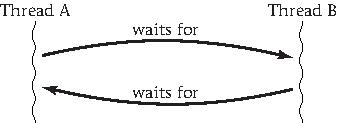
\includegraphics{hail_f0401}}
%\centerline{\epsfbox{scan-4-2.eps}}
\caption{Deadlock results when threads wait for one another in a
  complete cycle.  In this simple example, thread A is waiting for
  thread B, which is waiting for thread A.}
\label{scan-4-2}
\end{figure}
Because this pathology results from waiting, I
will address it and three of the most practical cures in Section~\ref{deadlock-section}, after
completing the study of waiting-based means of synchronization.

Waiting also interacts with scheduling (the topic of
Chapter~\ref{scheduling-chapter}) in some interesting ways.  In particular, unless special
precautions are taken, synchronization mechanisms can subvert priority
scheduling, allowing a low-priority thread to run while a
high-priority thread waits.  Therefore, in
Section~\ref{synchronization-and-scheduling-section}, I will briefly consider the
interactions between synchronization and scheduling, as well as what can be
done to tame them.

Although sections \ref{deadlock-section} and \ref{synchronization-and-scheduling-section} 
address the problems of deadlock and unwanted scheduling interactions, the root 
cause of these problems is also worth considering.
The underlying problem is that
one thread can block the progress of another thread, which is undesirable
even in the absence of such dramatic symptoms as deadlock.  After all, a blocked thread can't take
advantage of available processing power to produce useful results.  
Alternative, nonblocking synchronization techniques have become increasingly important
as the number of processor cores in a typical computer system has grown.
Section~\ref{nonblocking-synchronization-section} briefly addresses this topic, 
showing how data structures can safely support concurrent threads without ever blocking progress.

Finally, I conclude the chapter in
Section~\ref{synchronization-and-security-section} by looking at security issues related
to synchronization.  In particular, I show how subtle synchronization
bugs, which may nearly never cause a malfunction unless provoked, can
be exploited by an attacker in order to circumvent the system's normal
security policies.
After this concluding section, I provide exercises, programming and exploration projects, and notes.

Despite the wide range of synchronization-related topics I cover in
this chapter, there are two I leave for later chapters.
Atomic transactions are a particularly sophisticated and important
synchronization pattern, commonly encountered in middleware;
therefore, I devote Chapter~\ref{transactions-chapter} entirely to them.  Also,
explicitly passing a message between threads (for example, via a network)
provides synchronization as well as communication, because the message
cannot be received until after it has been transmitted.  Despite this
synchronization role, I chose to address various forms of message
passing in Chapters \ref{networking-chapter} and
\ref{distmid-chapter}, the chapters related to communication.

\section{Races and the Need for Mutual Exclusion}\label{races-section}

When two or more threads operate on a shared data structure, some very
strange malfunctions can occur if the timing of the threads turns out
precisely so that they
interfere with one another.  For example, consider the following
code that might appear in a \verb|sellTicket| procedure (for an event
without assigned seats):
\begin{verbatim}
if(seatsRemaining > 0){
  dispenseTicket();
  seatsRemaining = seatsRemaining - 1;
} else
  displaySorrySoldOut();
\end{verbatim}

On the surface, this code looks like it should never sell more tickets
than seats are available.  However, what happens if multiple threads
(perhaps controlling different points of sale) are executing the same
code?  Most of the time, all will be well.  Even if two people try to
buy tickets at what humans perceive as the same moment, on the time scale of
the computer, probably one will happen first and the other second, as
shown in Figure~\ref{ticket-ok-figure}.
\begin{figure}
\centerline{\begin{tabular}{|l|l|}
\hline\multicolumn{1}{|c|}{\bf Thread A} & \multicolumn{1}{c|}{\bf Thread B}\\\hline
\tt if(seatsRemaining > 0) & \\
\tt dispenseTicket(); & \\
\tt seatsRemaining=seatsRemaining-1; & \\
&\tt if(seatsRemaining > 0)...else \\
&\tt displaySorrySoldOut(); \\\hline
\end{tabular}}
\caption{Even if two humans think they are trying to buy the last
  ticket at the same time, chances are good that one's thread (thread A
  in this example) will run before the other's.  Thread B will then
  correctly discover that no seats remain.}\label{ticket-ok-figure}
\end{figure}
In that case, all is well.  However, once in a blue moon, the timing may be
exactly wrong, and the following scenario results, as shown in
Figure~\ref{ticket-race-figure}.
\begin{figure}
\centerline{\begin{tabular}{|l|l|}
\hline\multicolumn{1}{|c|}{\bf Thread A} & \multicolumn{1}{c|}{\bf Thread B}\\\hline
\tt if(seatsRemaining > 0) & \\
&\tt if(seatsRemaining > 0) \\
\tt dispenseTicket(); & \\
&\tt dispenseTicket(); \\
\tt seatsRemaining=seatsRemaining-1; & \\
&\tt seatsRemaining=seatsRemaining-1;  \\\hline
\end{tabular}}
\caption{If threads A and B are interleaved, both can act as though
  there were a ticket left to sell, even though only one really exists
  for the two of them.}\label{ticket-race-figure}
\end{figure}
\begin{enumerate}
\item
Thread A checks \verb|seatsRemaining > 0|.  Because
\verb|seatsRemaining| is 1, the test succeeds.  Thread A will take the
first branch of the \verb|if|.
\item
Thread B checks \verb|seatsRemaining > 0|.  Because
\verb|seatsRemaining| is 1, the test succeeds.  Thread B will take the
first branch of the \verb|if|.
\item
Thread A dispenses a ticket and decreases \verb|seatsRemaining| to 0.
\item
Thread B dispenses a ticket and decreases \verb|seatsRemaining| to $-1$.
\item
One customer winds up sitting on the lap of another.
\end{enumerate}

Of course, there are plenty of other equally unlikely scenarios that
result in misbehavior.  In Exercise~\ref{race-exercise}, you can come
up with a scenario
where, starting with \verb|seatsRemaining| being 2, two threads each
dispense a ticket, but \verb|seatsRemaining| is left as 1 rather than
0.

These scenarios are examples of \vocabs{race}.  In a race, 
two threads use the same data structure, without any mechanism to
ensure only one thread uses the data structure at a time.  If either thread precedes the
other, all is well.  However, if the two are interleaved, the program
malfunctions.  Generally, the malfunction can be expressed as some
invariant property being violated.  In the ticket-sales example, the
invariant is that the value of \verb|seatsRemaining|
should be nonnegative and when added to
the number
of tickets dispensed should equal the total number of seats.
(This invariant assumes that \verb|seatsRemaining| was initialized to
the total number of seats.)

When an invariant involves more than one variable, a race can result
even if one of the threads only reads the variables, without modifying
them.  For example, suppose there are two variables, one recording how
many tickets have been sold and the other recording the amount of
cash in the money drawer.  There should be an invariant relation between
these: the number of tickets sold times the price per ticket, plus the
amount of starting cash, should equal the cash on hand.  Suppose one
thread is in the midst of selling a ticket.  It has updated one of the
variables, but not yet the other.  If at exactly that moment another
thread chooses to run an audit function, which inspects the values of
the two variables, it will find them in an inconsistent state.

That inconsistency may not sound so terrible, but what if a similar
inconsistency occurred in a
medical setting, and one variable recorded the drug to administer,
while the other recorded the dose?  Can you see how dangerous an
inconsistency could be?  Something very much like that happened in a
radiation therapy machine, the \index{Therac-25}Therac-25, with occasionally lethal
consequences.  (Worse, some patients suffered terrible but not
immediately lethal injuries and lingered for some time in
excruciating, intractable pain.)

From the ticket-sales example, you can see that having two
threads carrying out operations on the same data structure is
harmless, as long as there never are two operations under way at the
same time.  In other words, the interleaving of the threads' execution
needs to be at the granularity of complete operations, such as selling
a ticket or auditing the cash drawer.  When interleaving the operations,
it's OK if one thread performs
several complete operations in a row; the threads don't need to alternate back and forth.
However, each sale or audit should be completed without interruption.

The reason why any interleaving of complete operations is safe is
because each is designed to both rely on the invariant and preserve
it.  Provided that you initially construct the data structure in a state
where the invariant holds, any sequence whatsoever of
invariant-preserving operations will leave the invariant intact.

What is needed, then, is a synchronization mechanism that allows one
thread to obtain private access to the data structure before it begins work, thereby
excluding all other threads from operating on that structure.  The
conventional metaphor is to say that the thread \vocabs{lock} the data structure.
When
the thread that locked the structure is done, it unlocks, allowing
another thread to take its turn.  Because any thread in the midst of
one of the operations temporarily excludes all the others,
this arrangement is called \foldvocab{mutual}{exclusion}.  Mutual exclusion establishes the
granularity at which threads may be interleaved by the scheduler.

\section{Mutexes and Monitors}\label{mutexes-and-monitors-section}

As you saw in Section~\ref{races-section}, threads that share data structures
need to have a mechanism for obtaining exclusive access to those
structures.  A programmer can arrange for this exclusive access by
creating a special lock object associated with each shared data
structure.  The lock can only be locked by one thread at a time.
A thread that has locked the lock is said to \vocabindex{hold}{hold (a lock)} the lock, even though that vocabulary has no obvious connection to the metaphor of real-world locks.
If
the threads operate on (or even examine) the data structure
only when holding the corresponding lock, this discipline will prevent
races.

To
support this form of race prevention, operating systems and middleware generally
provide mutual exclusion locks.  Because the name \foldvocab{mutual exclusion}{lock}
is rather ungainly, something shorter is generally used.  Some
programmers simply talk of \vocabs{lock}, but that can lead to confusion
because other synchronization mechanisms are also called locks. (For
example, I introduce readers/writers locks in Section~\ref{rw-section}.)  Therefore, the
name \vocab{mutex} has become popular as a shortened form of \foldvocab{mutual
exclusion}{lock}.  In particular, the POSIX standard refers to
mutexes.  Therefore, I will use that name in this book as well.

Section~\ref{mutex-api-section} presents the POSIX application
programming interface (API) for
mutexes. Section~\ref{monitors-section} presents an alternative, more
structured interface to mutexes, known as monitors.  Finally,
Section~\ref{mutex-mechanisms-section} shows what lies behind both
of those interfaces by explaining the mechanisms typically used to
implement mutexes.

\subsection{The Mutex Application Programing Interface}\label{mutex-api-section}

A mutex can be in either of two states: locked (that is, held by some
thread), or unlocked (that is, not held by any thread).  Any
implementation of mutexes must have some way to create a mutex and
initialize its state.  Conventionally, mutexes are initialized to the
unlocked state.  As a minimum, there must be two other operations: one
to lock a mutex, and one to unlock it.

The lock and unlock operations are much less symmetrical than they
sound.  The unlock operation can be applied only when the mutex is
locked; this operation does its job
and returns, without making the calling thread wait.  The lock
operation, on the other hand, can be invoked even when the lock is
already locked.  For this reason, the calling thread may need to wait, as shown in
Figure~\ref{scan-4-3}.
\begin{figure}
\centerline{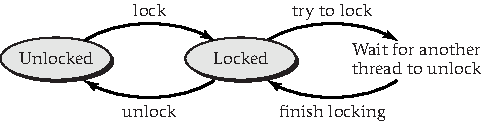
\includegraphics{hail_f0404}}
%\centerline{\epsfbox{scan-4-3.eps}}
\caption{Locking an unlocked mutex and unlocking a locked one change
  the mutex's state.  However, a thread can also try to lock an
  already-locked mutex.  In this case, the thread waits and acquires
  the mutex lock when another thread unlocks it.}
\label{scan-4-3}
\end{figure}
When a thread invokes the lock operation on a mutex, and that mutex is
already in the locked state, the thread is made to wait until another
thread has unlocked the mutex.  At that point, the thread that wanted
to lock the mutex can resume execution, find the mutex unlocked, lock
it, and proceed.

If more than one thread is trying to lock the same
mutex, only one of them will switch the mutex from unlocked to locked;
that thread will be allowed to proceed.  The others will wait until
the mutex is again unlocked.  This behavior of the lock operation
provides mutual exclusion.  For a thread to proceed past the point
where it invokes the lock operation, it must be the single thread that
succeeds in switching the mutex from unlocked to locked.  Until the
thread unlocks the mutex, one can say it \vocabindex{holds}{hold (a lock)} the mutex (that is, has
exclusive rights) and can safely operate on the associated data
structure in a race-free fashion.

This freedom from races exists regardless which one of the waiting
threads is chosen as the one to lock the mutex.  However, the question of
which thread goes first may matter for other reasons; I return to it
in Section~\ref{convoy-section}.

Besides the basic operations to initialize a mutex, lock it, and
unlock it, there may be other, less essential, operations as well.
For example, there may be one to test whether a mutex is immediately
lockable without waiting, and then to lock it if it is so.  For systems that
rely on manual reclamation of memory, there may also be an operation
to destroy a mutex when it will no longer be used.

Individual operating systems and middleware systems provide mutex APIs
that fit the general pattern I described, with varying details.
In order to see one concrete example of an API, I will present the
mutex operations included in the POSIX standard.  Because this is a
standard, many different operating systems provide this API, as well
as perhaps other system-specific APIs.

In the POSIX API, you can declare \verb|my_mutex| to be a mutex and
initialize it with the default attributes as follows:
\index{pthread_mutex_t@\verb"|pthread_mutex_t"|}%
\index{pthread_mutex_init@\verb"|pthread_mutex_init"|}%
\begin{verbatim}
pthread_mutex_t my_mutex;
pthread_mutex_init(&my_mutex, 0);
\end{verbatim}
A thread that wants to lock the mutex, operate on the associated data
structure, and then unlock the mutex would do the following (perhaps
with some error-checking added):
\index{pthread_mutex_lock@\verb"|pthread_mutex_lock"|}%
\index{pthread_mutex_unlock@\verb"|pthread_mutex_unlock"|}%
\begin{verbatim}
pthread_mutex_lock(&my_mutex);
// operate on the protected data structure
pthread_mutex_unlock(&my_mutex);
\end{verbatim}
As an example, Figure~\ref{tickets-pthreads-code} shows the key
procedures from the ticket sales example, written in C using the POSIX API.
\begin{figure}
\begin{verbatim}
void sellTicket(){
  pthread_mutex_lock(&my_mutex);
  if(seatsRemaining > 0){
    dispenseTicket();
    seatsRemaining = seatsRemaining - 1;
    cashOnHand = cashOnHand + PRICE;
  } else
    displaySorrySoldOut();
  pthread_mutex_unlock(&my_mutex);
}

void audit(){
  pthread_mutex_lock(&my_mutex);
  int revenue = (TOTAL_SEATS - seatsRemaining) * PRICE;
  if(cashOnHand != revenue + STARTING_CASH){
    printf("Cash fails to match.\n");
    exit(1);
  }
  pthread_mutex_unlock(&my_mutex);
}
\end{verbatim}
\caption{Each of these procedures begins by locking {\tt my\_mutex} and
  ends by unlocking it.  Therefore, they will never race, even if
  called from concurrent threads. Additional code not shown here
  (perhaps in the main procedure) would first initialize {\tt my\_mutex}.}
\label{tickets-pthreads-code}
\end{figure}
When all threads are done using the mutex (leaving it in the unlocked
state), the programmer is expected to destroy it, so that any
underlying memory can be reclaimed.  This is done by
executing the following procedure call:
\index{pthread_mutex_destroy@\verb"|pthread_mutex_destroy"|}%
\begin{verbatim}
pthread_mutex_destroy(&my_mutex);
\end{verbatim}

POSIX also provides a couple variants on \verb|pthread_mutex_lock|
that are useful under particular circumstances.  One,
\index{pthread_mutex_trylock@\verb"|pthread_mutex_trylock"|}\verb|pthread_mutex_trylock|, differs in that it will never wait to
acquire a mutex. Instead, it returns an error code if unable to
immediately acquire the lock.  The other,
\index{pthread_mutex_timedlock@\verb"|pthread_mutex_timedlock"|}\verb|pthread_mutex_timedlock|, allows the programmer to specify a
maximum amount of time to wait.  If the mutex cannot be acquired
within that time, \verb|pthread_mutex_timedlock| returns an error
code.

Beyond their wide availability, another reason why POSIX mutexes are
worth studying is that the programmer is allowed to choose among several
variants, which provide different answers to two questions about exceptional
circumstances.
Other mutex APIs might include one specific answer to these questions,
rather than exposing the full range of possibilities.  The questions
at issue are as follows:
\begin{itemize}
\item
What happens if a thread tries to unlock a mutex that is unlocked, or that was locked by a
different thread?
\item
What happens if a thread tries to lock a mutex that it already holds?
(Note that if the thread were to wait for itself to unlock the mutex,
this situation would constitute the simplest possible case of a deadlock.  The cycle of
waiting threads would consist of a single thread, waiting for itself.)
\end{itemize}

The POSIX standard allows the programmer to select from four different
types of mutexes, each of which answers these two questions in a
different way:
\begin{description}
\item[\texttt{PTHREAD\_MUTEX\_DEFAULT}]
If a thread tries to
lock a mutex it already holds or unlock one it doesn't hold, all bets are off as to what will happen.
The programmer has a responsibility never to make either of these attempts.
Different POSIX-compliant systems may behave differently.
\item[\texttt{PTHREAD\_MUTEX\_ERROR\_CHECK}]
If a thread tries to lock a mutex that it already holds, or unlock a
mutex that it doesn't hold, the operation returns an error code.
\item[\texttt{PTHREAD\_MUTEX\_NORMAL}]
If a thread tries to lock a mutex that it already holds, it goes into
a deadlock situation, waiting for itself to unlock the mutex, just
as it would wait for any other thread.  If a thread tries to unlock
a mutex that it doesn't hold, all bets are off; each POSIX-compliant
system is free to respond however it likes.
\item[\texttt{PTHREAD\_MUTEX\_RECURSIVE}]
If a thread tries to unlock a mutex that it doesn't hold, the
operation returns an error code.  If a thread tries to lock a mutex
that it already holds, the system simply increments a count of how
many times the thread has locked the mutex and allows the thread to
proceed.  When the thread invokes the unlock operation, the counter is
decremented, and only when it reaches 0 is the mutex really unlocked.
\end{description}

If you want to provoke a debate among experts on concurrent
programming, ask their opinion of \vocab{recursive locking}, that is,
of the mutex behavior specified by the POSIX option \texttt{PTHREAD\_MUTEX\_RECURSIVE}.
On the one hand, recursive locking gets rid of one especially silly
class of deadlocks, in which a thread waits for a mutex it already holds.
On the other hand, a programmer with recursive locking available may
not follow as disciplined a development approach. In particular, the programmer
may not keep track of exactly which locks are held at each point
in the program's execution.

\subsection{Monitors: A More Structured Interface to Mutexes}\label{monitors-section}

Object-oriented programming involves packaging together data
structures with the procedures that operate on them.  In this context,
mutexes can be used in a very rigidly structured way:
\begin{itemize}
\item
All state variables within an object should be kept private, accessible only to
code associated with that object.
\item
Every object (that might be shared between threads) should contain a
mutex as an additional field, beyond those fields containing the object's
state.
\item
Every method of an object (except private ones used internally) should
start by locking that object's mutex and end by unlocking the mutex
immediately before returning.
\end{itemize}
If these three rules are followed, then it will be impossible for two
threads to race on the state of an object, because all access to the
object's state will be protected by the object's mutex.

Programmers can follow these rules manually, or the programming
language can provide automatic support for the rules.  Automation
ensures that the rules are consistently followed.  It also means the
source program will not be cluttered with mutex clich{\'e}s, and hence
will be more readable.

An object that automatically follows the mutex rules is called a
\vocab{monitor}.  Monitors are found in some programming languages,
such as Concurrent Pascal, that
have been used in research settings without becoming commercially
popular.  In these languages, using monitors can be as simple as using
the keyword \verb|monitor| at the
beginning of a declaration for a class of objects.  All public methods
will then automatically lock and unlock an automatically supplied
mutex.  (Monitor languages also support another synchronization
feature, condition variables, which I discuss in Section~\ref{condition-variables-section}.)


Although true monitors have not become popular, the Java programming
language provides a close approximation.  To achieve monitor-style
synchronization, the Java programmer needs to exercise some self-discipline, but less than with raw mutexes.  More importantly, the
resulting Java program is essentially as uncluttered as a true monitor
program would be; all that is added is one keyword,
\verb|synchronized|, at the declaration of each nonprivate method.

Each Java object automatically has a mutex associated with it, of the
recursively lockable kind.  The programmer can choose to lock any
object's mutex for the duration of any block of code by using a
\index{synchronized statement@\verb"|synchronized"| statement}\verb|synchronized| statement:
\begin{verbatim}
synchronized(someObject){
  // the code to do while holding someObject's mutex
}
\end{verbatim}
Note that in this case, the code need not be operating on the state of
\verb|someObject|; nor does this code need to be in a method
associated with that object.  In other words, the \verb|synchronized|
statement is essentially as flexible as using raw mutexes, with the
one key advantage that locking and unlocking are automatically paired.
This advantage is important, because it eliminates one big class of
programming errors.  Programmers often forget to unlock mutexes under
exceptional circumstances.  For example, a procedure may lock a mutex
at the beginning and unlock it at the end.  However, in between may
come an \verb|if| statement that can terminate the procedure with
the mutex still locked.

Although the \verb|synchronized|
statement is flexible, typical Java programs don't use it much.  Instead, programmers add the keyword
\index{synchronized method@\verb"|synchronized"| method}\verb|synchronized| to the declaration of public methods.  For
example, a \verb|TicketVendor| class might follow the outline in
Figure~\ref{TicketVendor}.
\begin{figure}
\begin{verbatim}
public class TicketVendor {
  private int seatsRemaining, cashOnHand;
  private static final int PRICE = 1000;

  public synchronized void sellTicket(){
    if(seatsRemaining > 0){
      dispenseTicket();
      seatsRemaining = seatsRemaining - 1;
      cashOnHand = cashOnHand + PRICE;
    } else
      displaySorrySoldOut();
  }

  public synchronized void audit(){
    // check seatsRemaining, cashOnHand
  }

  private void dispenseTicket(){
    // ...
  }

  private void displaySorrySoldOut(){
    // ...
  }

  public TicketVendor(){
    // ...
  }
}
\end{verbatim}
\caption{Outline of a monitor-style class in Java}
\label{TicketVendor}
\end{figure}
Marking a method \verb|synchronized| is
equivalent to wrapping the entire body of that method in
a \verb|synchronized| statement:
\begin{verbatim}
synchronized(this){
  // the body
}
\end{verbatim}
In other words, a synchronized method on an object will be executed
while holding that object's mutex.  For example, the \verb|sellTicket|
method is synchronized, so if two different threads invoke it, one
will be served while the other waits its turn, because the
\verb|sellTicket| method is implicitly locking a mutex upon entry and
unlocking it upon return, just as was done explicitly in the POSIX
version of Figure~\ref{tickets-pthreads-code}.  Similarly, a thread
executing the \verb|audit| method will need to wait until no ticket
sale is in progress, because this method is also marked synchronized,
and so acquires the same mutex.

In order to program in a monitor style in Java, you need to be
disciplined in your use of the \verb|private| and \verb|public|
keywords (including making all state \verb|private|), and you need to
mark all the public methods as \verb|synchronized|.

\subsection{Underlying Mechanisms for Mutexes}\label{mutex-mechanisms-section}

In this subsection, I will show how mutexes typically operate behind
the scenes.  I start with a version that functions correctly, but is
inefficient, and then show how to build a more efficient version on
top of it, and then a yet more efficient version on top of that.  Keep
in mind that I will not throw away my first two versions: they play
a critical role in the final version.  For simplicity, all three
versions will be of the \texttt{PTHREAD\_MUTEX\_NORMAL} kind;
a deadlock results if a thread tries to lock a mutex it already
holds.  In Exercise~\ref{recursive-mutex-exercise},
you can figure out the changes needed for \texttt{PTHREAD\_MUTEX\_RECURSIVE}.

The three versions of mutex are called the basic spinlock,
cache-conscious spinlock, and queuing mutex, in increasing order of
sophistication.  The meaning of these names will become apparent as I
explain the functioning of each kind of mutex.  I will start with the
basic spinlock.

All modern processor architectures have at least one instruction that
can be used to both change the contents of a memory location and
obtain information about the previous contents of the location.
Crucially, these instructions are executed \vocabindex{atomically}{atomic}, that is, as
an indivisible unit that cannot be broken up by the arrival of an
interrupt nor interleaved with the execution of an instruction on
another processor.  The details of these instructions vary; for
concreteness, I will use the \vocab{exchange} operation, which atomically
swaps the contents of a register with the contents of a memory
location.

Suppose I represent a basic spinlock as a memory location that contains 1 if
the mutex is unlocked and 0 if the mutex is locked.  The unlock
operation can be trivial: to unlock a mutex, just store 1 into it.
The lock operation is a bit trickier and uses the atomic exchange
operation; I can express it in pseudocode, as shown in
Figure~\ref{basic-spinlock-lock}.
\begin{figure}
\begin{verbatim}
to lock mutex:
  let temp = 0
  repeat
    atomically exchange temp and mutex
  until temp = 1
\end{verbatim}
\caption{The basic spinlock version of a mutex is a memory location
  storing 1 for unlocked and 0 for locked.  Locking the mutex consists of
  repeatedly exchanging a register containing 0 with the memory
  location until the location is changed from 1 to 0.}
\label{basic-spinlock-lock}
\end{figure}
The key idea here is to keep looping until the thread succeeds in changing the
mutex from 1 to 0.  So long as some other thread holds the
lock, the thread keeps swapping one 0 with another 0, which does no harm.
This process is illustrated in Figure~\ref{scan-4-4}.
\begin{figure}
\centerline{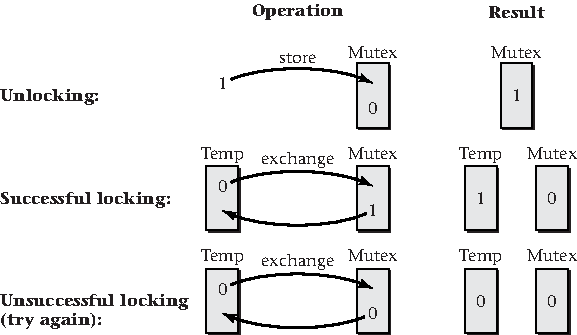
\includegraphics{hail_f0408}}
%\centerline{\epsfbox{scan-4-4.eps}}
\caption{Unlocking a basic spinlock consists of storing a 1 into it.
  Locking it consists of storing a 0 into it using an atomic exchange
  instruction.  The exchange instruction allows the locking thread to verify that the
  value in memory really was changed from 1 to 0.  If not, the thread
  repeats the attempt.}
\label{scan-4-4}
\end{figure}

To understand the motivation behind the cache-conscious spinlock, you need to
know a little about \foldindex{cache}{coherence}cache coherence
protocols in \index{multiprocessor system}multiprocessor
systems.  Copies of a given block of memory can reside in several
different processors' caches, as long as the processors only read from the
memory locations.  As soon as one processor wants to write into the
cache block, however, some communication between the caches is
necessary so that other processors don't read out-of-date
values.  Most typically, the cache where the writing occurs invalidates all the other caches' copies so
that it has exclusive ownership.  If one of the other processors now
wants to write, the block needs to be flushed out of the first cache
and loaded exclusively into the second.  If the two processors keep
alternately writing into the same block, there will be continual
traffic on the memory interconnect as the cache block is transferred
back and forth between the two caches.

This is exactly what will happen with the basic spinlock version of mutex
locking if two threads (on two processors) are both waiting for the
same lock.  The atomic exchange instructions on the two processors will
both be writing into the cache block containing the spinlock.
Contention for a mutex may not
happen often.  When it does, however, the performance will be
sufficiently terrible to motivate an improvement. Cache-conscious spinlocks
will use the same simple approach as basic spinlocks  when there is no
contention, but will get rid of the cache coherence traffic while waiting
for a contended mutex.

In order to allow multiple processors to wait for a lock without
generating traffic outside their individual caches, they must be
waiting while using only reads of the mutex.  When they see the mutex become
unlocked, they then need to try grabbing it with an atomic
exchange.  This approach leads to the pseudocode shown in Figure~\ref{cache-conscious-lock}.
\begin{figure}
\begin{verbatim}
to lock mutex:
  let temp = 0
  repeat
    atomically exchange temp and mutex
    if temp = 0 then
      while mutex = 0
        do nothing
  until temp = 1
\end{verbatim}
\caption{Cache-conscious spinlocks are represented the same way as
  basic spinlocks, using a single memory location.  However, the lock
  operation now uses ordinary read instructions in place of most of
  the atomic exchanges while waiting for the mutex to be unlocked.}
\label{cache-conscious-lock}
\end{figure}
Notice that in the common case where the mutex can be acquired
immediately, this version acts just like the original.  Only if the
attempt to acquire the mutex fails is anything done differently.  Even
then, the mutex will eventually be acquired the same way as before.

The two versions of mutexes that I have presented thus far share one
key property, which explains why both are called spinlocks.
They both engage in \foldindex{busy}{waiting}busy waiting if the mutex
is not immediately available.  Recall from my discussion of scheduling
that busy waiting means waiting by continually executing instructions
that check for the awaited event.  A mutex that uses busy waiting is
called a \vocab{spinlock}.  Even fancier versions of spinlocks exist,
as described in the end-of-chapter notes.

The alternative to busy waiting is to notify the operating system that
the thread needs to wait.  The operating system can then change the
thread's state to waiting and move it to a
wait queue, where it is not eligible for time on the processor.
Instead, the scheduler will use the processor to run other threads.
When the mutex is unlocked, the waiting thread can be made runnable
again.  Because this form of mutex makes use of a wait queue, it is
called a queuing mutex.

Spinlocks are inefficient, for the same reason as any busy waiting is inefficient.
The thread does not make any more headway, no matter how many times it
spins around its loop.  Therefore, using the processor for a different
thread would benefit that other thread without harming the waiting
one.

However, there is one flaw in this argument.  There is some overhead
cost for notifying the operating system of the desire to wait,
changing the thread's state, and doing a context switch, with the
attendant loss of cache locality.  Thus, in a situation where the
spinlock needs to spin only briefly before finding the mutex unlocked,
the thread might actually waste less time busy waiting than it would waste
getting out of other threads' ways.  The relative efficiency of
spinlocks and queuing mutexes
depends on how long the thread needs to wait before the
mutex becomes available.

For this reason, spinlocks are appropriate to use for mutexes that are
held only very briefly, and hence should be quickly acquirable.
As an example, the Linux kernel uses spinlocks to protect many of its
internal data structures during the brief operations on them.  For
example, I mentioned that the scheduler keeps the runnable threads in
a run queue.  Whenever the scheduler wants to
insert a thread into this data structure, or otherwise operate on
it, it locks a spinlock, does the brief operation, and then
unlocks the spinlock.

Queuing mutexes are still needed for those cases where a
thread might hold a mutex a long time---long enough that other
contenders shouldn't busy wait.  These mutexes will be more complex.
Rather than being stored in a single memory location (as with
spinlocks), each mutex will have three components:
\begin{itemize}
\item
A memory location used to record the mutex's state, 1 for unlocked or
0 for locked.
\item
A list of threads waiting to acquire the mutex.  This list is what
allows the scheduler to place the threads in a waiting state, instead
of busy waiting.  Using the terminology of
Chapter~\ref{scheduling-chapter}, this list is a wait queue.
\item
A cache-conscious spinlock, used to protect against races in
operations on the mutex itself.
\end{itemize}
In my pseudocode, I will refer to these three components as
\verb|mutex.state|, \verb|mutex.waiters|, and \verb|mutex.spinlock|,
respectively.

Under these assumptions, the locking and unlocking operations can be
performed as shown in the pseudocode of Figures \ref{lock-pseudo-code} and
\ref{unlock-pseudo-code}.  Figures \ref{scan-4-5} and \ref{scan-4-6}
illustrate the functioning of these operations.
\begin{figure}
\begin{verbatim}
to lock mutex:
  lock mutex.spinlock (in cache-conscious fashion)
  if mutex.state = 1 then
    let mutex.state = 0
    unlock mutex.spinlock
  else
    add current thread to mutex.waiters
    remove current thread from runnable threads
    unlock mutex.spinlock
    yield to a runnable thread
\end{verbatim}
\caption{An attempt to lock a queuing mutex that is already in the
  locked state causes the thread to join the wait queue, {\tt mutex.waiters}.}
\label{lock-pseudo-code}
\end{figure}
\begin{figure}
\begin{verbatim}
to unlock mutex:
  lock mutex.spinlock (in cache-conscious fashion)
  if mutex.waiters is empty then
    let mutex.state = 1
  else
    move one thread from mutex.waiters to runnable
  unlock mutex.spinlock
\end{verbatim}
\caption{If there is any waiting thread, the unlock operation on a queuing mutex causes a thread to become
  runnable. Note that in this case, the mutex is left in the locked
  state; effectively, the locked mutex is being passed directly from
  one thread to another.}
\label{unlock-pseudo-code}
\end{figure}
\begin{figure}
\centerline{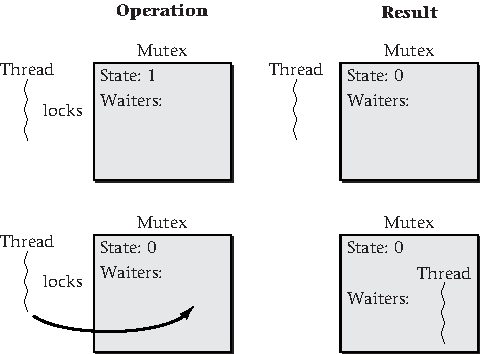
\includegraphics{hail_f0412}}
%\centerline{\epsfbox{scan-4-5.eps}}
\caption{Locking a queuing mutex that is unlocked simply changes the
  mutex's state.  Locking an already-locked queuing mutex, on the
  other hand, puts the thread into the waiters list.}
\label{scan-4-5}
\end{figure}
\begin{figure}
\centerline{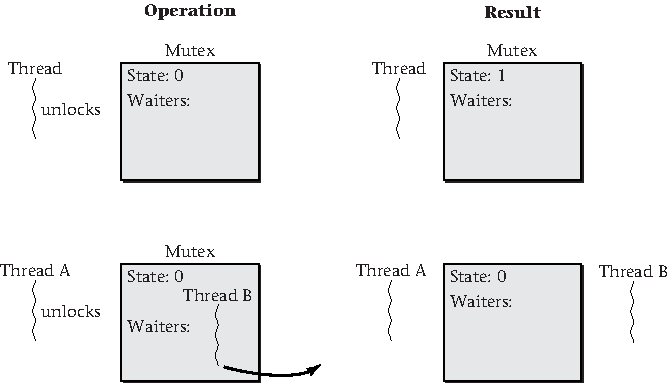
\includegraphics{hail_f0413}}
%\centerline{\epsfbox{scan-4-6.eps}}
\caption{Unlocking a queuing mutex with no waiting threads simply
  changes the mutex's state.  Unlocking a queuing mutex with waiting
  threads, on the other hand, leaves the state set to locked but
  causes one of the waiting threads to start running again, having
  acquired the lock.}
\label{scan-4-6}
\end{figure}
One important feature to note in this mutex design concerns what
happens when a thread performs the unlock operation on a mutex that has one or more threads in the
waiters list.  As you can see in Figure~\ref{unlock-pseudo-code}, the
mutex's state variable is not changed from the locked state (0) to the
unlocked state (1).  Instead, the mutex is left locked, and one of the
waiting threads is woken up.  In other words, the locked mutex is
passed directly from one thread to another, without ever really being
unlocked.  In Section~\ref{convoy-section}, I will explain how this
design is partially responsible for the so-called convoy
phenomenon, which I describe there.  In that same section, I will also present an
alternative design for mutexes that puts the mutex into the unlocked
state.

\section{Other Synchronization Patterns}\label{other-synchronization-problems-section}

Recall that synchronization refers to any form of control over the
relative timing of two or more threads.  As such, synchronization
includes more than just mutual exclusion; a programmer may want to impose some
restriction on relative timing other than the rule of one thread at a
time.  In this section, I present three other patterns of
synchronization that crop up over and over again in many applications:
bounded buffers, readers/writers locks, and barriers.
Sections \ref{bounded-buffers-section} through 
\ref{barriers-section} will just describe the desired synchronization;
Sections \ref{condition-variables-section} and \ref{semaphores-section} show techniques that can be used to achieve the
synchronization.

\subsection{Bounded Buffers}\label{bounded-buffers-section}

Often, two threads are linked together in a processing
\vocab{pipeline}.  That is,
the first thread produces a sequence of values that are consumed by
the second thread.  For example, the first thread may be extracting
all the textual words from a document (by skipping over the formatting
codes) and passing those words to a second thread that speaks the
words aloud.

One simple way to organize the processing would be by strict
alternation between the producing and consuming threads.  In the preceding
example, the first thread would extract a word, and then wait while
the second thread converted it into sound.  The second thread would
then wait while the first thread extracted the next word.  However,
this approach doesn't yield any concurrency: only one thread is
runnable at a time.  This lack of concurrency may result in suboptimal
performance if the computer system has two processors, or
if one of the threads spends a lot of time waiting for an I/O device.

Instead, consider running the \index{producer}producer and the \index{consumer}consumer
concurrently.  Every time the producer has a new value ready, the producer will
store the value into an intermediate storage area, called a \vocab{buffer}.
Every time the consumer is ready for the next value, it will retrieve
the value from the buffer.  Under normal circumstances, each can operate at
its own pace.  However, if the consumer goes to the buffer to retrieve
a value and finds the buffer empty, the consumer will need to wait for the
producer to catch up.  Also, if you want to limit the size of the
buffer (that is, to use a \foldvocab{bounded}{buffer}), you need to make the producer wait
if it gets too far ahead of the consumer and fills the buffer.  Putting
these two synchronization restrictions in place ensures that over the
long haul, the rate of the two threads will match up, although
over the short term, either may run faster than the other.

You should be familiar with the bounded buffer pattern from businesses
in the real world.  For example, the cooks at a fast-food
restaurant fry burgers concurrently with the cashiers selling them.
In between the two is a bounded buffer of already-cooked burgers.
The exact number of burgers in the buffer will grow or shrink somewhat
as one group of workers is temporarily a little faster than the
other.  Only under extreme circumstances does one group of workers
have to wait for the other.  Figure~\ref{scan-4-7} illustrates a situation where no one needs to wait.
\begin{figure}
\centerline{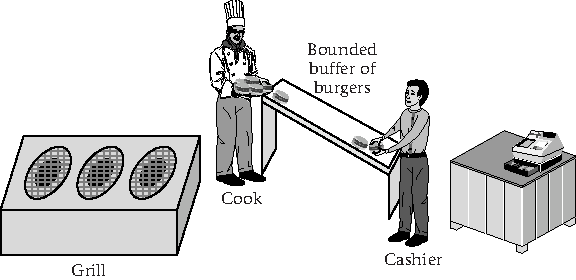
\includegraphics{hail_f0414}}
%\centerline{\epsfbox{scan-4-7.eps}}
\caption{A cook fries burgers and places them in a bounded buffer,
  queued up for later sale.  A cashier takes burgers from the
  buffer to sell.  If there are none available, the cashier waits.
  Similarly, if the buffer area is full, the cook takes a break from
  frying burgers.}
\label{scan-4-7}
\end{figure}


One easy place to see bounded buffers at work in computer systems is
the \vocab{pipe} feature built into UNIX-family operating systems,
including Linux and Mac OS~X.  (Microsoft Windows also now has an
analogous feature.)  Pipes allow the output produced by one process to
serve as input for another.  For example, on a Mac OS~X
system, you could open a terminal window with a shell in it and give the following command:
\begin{verbatim}
ls | say
\end{verbatim}
This runs two programs concurrently.  The first, \verb|ls|,
lists
the files in your current directory. 
The second one, \verb|say|, converts its textual input into speech and
plays it over the computer's speakers.   In the shell
command, the vertical bar character (\verb:|:) indicates the pipe from
the first program to the second. The net result is a spoken
listing of your files.

A more mundane version of this
example works not only on Mac OS~X, but also on other UNIX-family
systems such as Linux:
\begin{verbatim}
ls | tr a-z A-Z
\end{verbatim}
Again, this runs two programs concurrently.  This time the second one, \verb|tr|, copies
characters from its input to its output, with some changes
(transliterations) along the way; in this case, replacing lowercase
letters \verb|a-z| with the corresponding uppercase letters \verb|A-Z|.  The net
result is an uppercase listing of your files.  The file listing may
get ahead of the transliteration, as long as it doesn't overflow a
buffer the operating system provides for the pipe.  Once there is a
backlog of listed files in the buffer, the transliteration can run as
fast as it wants until it exhausts that backlog.

\subsection{Readers/Writers Locks}\label{rw-section}

My next example of a synchronization pattern is actually quite
similar to mutual exclusion.  Recall that in the ticket-sales
example, the audit function needed to acquire the mutex, even though auditing
is a read-only operation, in order to make sure that the audit read a consistent
combination of state variables.  That design achieved correctness, but
at the cost of needlessly limiting concurrency: it prevented two
audits from being underway at the same time, even though two (or more)
read-only operations cannot possibly interfere with each other.
My goal now is to rectify that problem.

A \foldvocab{readers/writers}{lock} is much like a mutex, except that when a thread
locks the lock, it specifies whether it is planning to do any writing
to the protected data structure
or only reading from it.  Just as with a mutex, the lock operation may not
immediately complete; instead, it waits until such time as the lock
can be acquired.  The difference is that any number of readers can
hold the lock at the same time, as shown in Figure~\ref{scan-4-8}; they will not wait for each other.  A
reader will wait, however, if a writer holds the lock.  A writer will
wait if the lock is held by any other thread, whether by another
writer or by one or more readers.
\begin{figure}
\centerline{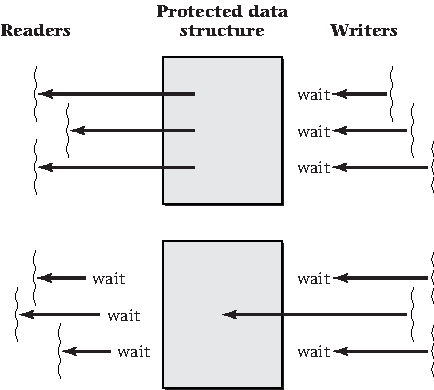
\includegraphics{hail_f0415}}
%\centerline{\epsfbox{scan-4-8.eps}}
\caption{A readers/writers lock can be held either by
  any number of readers or by one writer.  When the lock is held by
  readers, all the reader threads can read the protected data
  structure concurrently.}
\label{scan-4-8}
\end{figure}

Readers/writers locks are particularly valuable in situations where
some of the read-only operations are time consuming, as when reading a
file stored on disk.  This is especially true if many readers are
expected.  The choice between a mutex and a readers/writers lock is a
performance trade-off.  Because the mutex is simpler, it has lower
overhead.  However, the readers/writers lock may pay for its overhead
by allowing more concurrency.

One interesting design question arises if a readers/writers lock is
held by one or more readers and has one or more writers
waiting. Suppose a new reader tries to acquire the lock.  Should it be
allowed to, or should it be forced to wait until after the writers?
On the surface, there seems to be no reason for the reader to wait,
because it can coexist with the existing readers, thereby achieving
greater concurrency.  The problem is that an overlapping succession of
readers can keep the writers waiting arbitrarily long. The writers
could wind up waiting even when the only remaining readers arrived
long after the writers did.  This is a form of \vocab{starvation}, in
that a thread is unfairly prevented from running by other threads.  To
prevent this particular kind of starvation,
some versions of readers/writers locks make new readers wait until
after the waiting writers.

In Section~\ref{condition-variables-section}, you will learn how you
could build readers/writers locks
from more primitive synchronization mechanisms.  However,
because readers/writers locks are so generally useful, they are already
provided by many systems, so you may never actually have to build them
yourself.  The POSIX standard, for example, includes readers/writers
locks with procedures such as \index{pthread_rwlock_init@\verb"|pthread_rwlock_init"|}\verb|pthread_rwlock_init|,
\index{pthread_rwlock_rdlock@\verb"|pthread_rwlock_rdlock"|}\verb|pthread_rwlock_rdlock|, \index{pthread_rwlock_wrlock@\verb"|pthread_rwlock_wrlock"|}\verb|pthread_rwlock_wrlock|, and
\index{pthread_rwlock_unlock@\verb"|pthread_rwlock_unlock"|}\verb|pthread_rwlock_unlock|.  The POSIX standard leaves it up to each
individual system how to prioritize new readers versus waiting
writers.

The POSIX standard also includes a more specialized form of
readers/writers locks specifically associated with files.  This
reflects my earlier comment that readers/writers locking is
especially valuable when reading may be time consuming, as with a file
stored on disk.  In the POSIX standard, file locks are available only
through the complex \index{fcntl@\verb"|fcntl"|}\verb|fcntl| procedure.  However, most UNIX-family
operating systems also provide a simpler interface, \index{flock@\verb"|flock"|}\verb|flock|.

\subsection{Barriers}\label{barriers-section}

\vocabindex{Barrier synchronization}{barrier synchronization}\index{synchronization, barrier} is the last common synchronization pattern I
will discuss.  Barriers are most commonly used in programs that do
large-scale numerical calculations for scientific or engineering
applications, such as simulating ocean currents.  However, they may
also crop up in other applications, as long as there is a requirement
for all threads in a group to finish one phase of the computation
before any of them moves on to the next phase.  In scientific
computations, the threads are often dividing up the processing of a
large matrix.  For example, ten threads may each process 200 rows of a
2000-row matrix.  The requirement for all threads to finish one phase
of processing before starting the next comes from the fact that the
overall computation is a sequence of matrix operations; parallel
processing occurs only within each matrix operation.

When a barrier is created (initialized), the programmer specifies how
many threads will be sharing it.  Each of the threads completes the first
phase of the computation and then invokes the barrier's wait
operation.  For most of the threads, the wait operation does not
immediately return; therefore, the thread calling it cannot
immediately proceed.  The one exception is whichever thread is the
last to call the
wait operation.  The barrier can tell which thread is the last one,
because the programmer specified how many threads there are.  When this last
thread invokes the wait operation, the wait operation immediately
returns.  Moreover, all the other waiting threads finally have their
wait operations also return, as illustrated in Figure~\ref{scan-4-9}.
\begin{figure}
\centerline{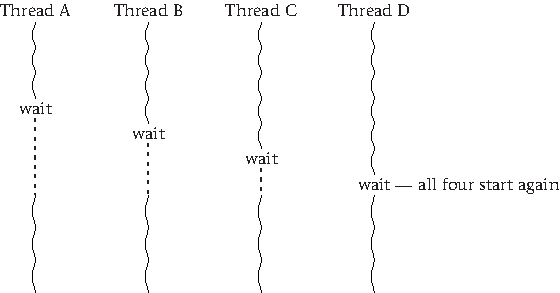
\includegraphics{hail_f0416}}
%\centerline{\epsfbox{scan-4-9.eps}}
\caption{A barrier is created for a specific number of threads.
In this case, there are
  four.  When the last of those threads invokes the wait operation,
  all the waiting threads in the group start running again.}
\label{scan-4-9}
\end{figure}
Thus, they can now all proceed on to the
second phase of the computation.  Typically, the same barrier can then
be reused between the second and third phases, and so forth.  (In other words,
the barrier reinitializes its state once it releases all the waiting
threads.)

Just as with readers/writers locks, you will see how barriers can be
defined in terms of more general synchronization mechanisms.  However,
once again there is little reason to do so in practice, because barriers
are provided as part of POSIX and other widely available APIs.

\section{Condition Variables}\label{condition-variables-section}

In order to solve synchronization problems, such as the three described
in Section~\ref{other-synchronization-problems-section},
you need some mechanism that allows a thread to wait
until circumstances are appropriate for it to proceed.  A producer may
need to wait for buffer space, or a consumer may need to wait for
data.  A reader may need to wait until a writer has unlocked, or a
writer may need to wait for the last reader to unlock.  A thread that
has reached a barrier may need to wait for all the other threads to do
so.  Each situation has its own condition for which a thread must
wait, and there are many other application-specific conditions
besides.  (A video playback that has been paused might wait until the
user presses the pause button again.)

All these examples can be handled by using \vocabs{condition variable}, a
synchronization mechanism that works in partnership with \index{monitor}monitors or
with mutexes used in the style of monitors.  There are two basic
operations on a condition variable: \vocab{wait} and \vocab{notify}.  (Some systems
use the name \vocab{signal} instead of notify.)  A thread that finds
circumstances not to its liking executes the wait operation and
thereby goes to sleep until such time as another thread invokes the
notify operation.  For example, in a bounded buffer, the producer
might wait on a condition variable if it finds the buffer full.  The
consumer, upon freeing up some space in the buffer, would invoke the
notify operation on that condition variable.

Before delving into all the important details and variants,
a concrete example may be helpful.  Figure~\ref{BoundedBuffer.java} shows the Java
code for a \index{BoundedBuffer class@\verb"|BoundedBuffer"|
class}\verb|BoundedBuffer| class.
\begin{figure}
\begin{verbatim}
public class BoundedBuffer {
  private Object[] buffer = new Object[20]; // arbitrary size
  private int numOccupied = 0;
  private int firstOccupied = 0;

  /* invariant: 0 <= numOccupied <= buffer.length
     0 <= firstOccupied < buffer.length
     buffer[(firstOccupied + i) % buffer.length]
     contains the (i+1)th oldest entry,
     for all i such that 0 <= i < numOccupied  */

  public synchronized void insert(Object o)
    throws InterruptedException
  {
    while(numOccupied == buffer.length)
      // wait for space
      wait();
    buffer[(firstOccupied + numOccupied) % buffer.length] = o;
    numOccupied++;
    // in case any retrieves are waiting for data, wake them
    notifyAll();
  }

  public synchronized Object retrieve()
    throws InterruptedException
  {
    while(numOccupied == 0)
      // wait for data
      wait();
    Object retrieved = buffer[firstOccupied];
    buffer[firstOccupied] = null; // may help garbage collector
    firstOccupied = (firstOccupied + 1) % buffer.length;
    numOccupied--;
    // in case any inserts are waiting for space, wake them
    notifyAll();
    return retrieved;
  }
}
\end{verbatim}
\caption{{\tt BoundedBuffer} class using monitors and condition variables}
\label{BoundedBuffer.java}
\end{figure}

Before I explain how this example works, and then return to a more
general discussion of condition variables, you should take a moment to
consider how you would test such a class.  First, it might help to
reduce the size of the buffer, so that all qualitatively different
situations can be tested more quickly.  Second, you need a test program
that has multiple threads doing insertions and retrievals, with some
way to see the difference between when each operation is started and
when it completes.  In the case of the retrievals, you will also need
to see that the retrieved values are correct.  Designing such a test
program is surprisingly interesting; you can have this experience in Programming Project~\ref{bounded-buffer-test-project}.

In Java, each object has a single condition variable automatically
associated with it, just as it has a mutex.  The \index{wait@\verb"|wait"|}\verb|wait| method
waits on the object's condition variable, and the \index{notifyAll@\verb"|notifyAll"|}\verb|notifyAll|
method wakes up all threads waiting on the object's condition
variable.  Both of these methods need to be called by a thread that
holds the object's mutex.  In my \verb|BoundedBuffer| example, I
ensured this in a straightforward way by using \verb|wait| and
\verb|notifyAll| inside methods that are marked \verb|synchronized|.

Having seen that \verb|wait| and \verb|notifyAll| need to be called
with the mutex held, you may spot a problem.  If a waiting thread
holds the mutex, there will be no way for any other thread to acquire
the mutex, and thus be able to call \verb|notifyAll|.  Until you learn
the rest of the story, it seems as though any thread that invokes
\verb|wait| is doomed to eternal waiting.

The solution to this dilemma is as follows.  When a thread invokes the
wait operation, it must hold the associated mutex.  However, the wait
operation releases the mutex before putting the thread into its
waiting state.  That way, the mutex is available to a potential waker.
When the waiting thread is awoken, it reacquires the mutex before the
wait operation returns.  (In the case of recursive mutexes, as used in
Java, the awakening thread reacquires the mutex with the same lock
count as before, so that it can still do just as many unlock
operations.)

The fact that a waiting thread temporarily releases the mutex helps
explain two features of the \verb|BoundedBuffer| example.  First, the waiting
is done at the very beginning of the methods.  This ensures that the
invariant is still intact when the mutex is released.  (More
generally, the waiting could happen later, as long as no state
variables have been updated, or even as long as they have been put
back into an invariant-respecting state.)  Second, the waiting is done
in a loop; only when the waited-for condition has been verified to
hold does the method move on to its real work.  The loop is essential
because an awoken thread needs to reacquire the mutex, contending with
any other threads that are also trying to acquire the mutex.  There is
no guarantee that the awoken thread will get the mutex first.  As
such, there is no guarantee what state it will find; it may need to
wait again.

When a waiting thread releases the mutex in order to wait on the
condition variable, these two actions are done indivisibly.  There is
no way another thread can acquire the mutex before the first thread
has started waiting on the condition variable.  This ensures no other
thread will do a notify operation until after the thread that wants to
wait is actually waiting.

In addition to waiting for appropriate conditions at the top of each
method, I have invoked \verb|notifyAll| at the end of each
method.  This position is less crucial, because the \verb|notifyAll|
method does not release the mutex.  The calling thread continues to
hold the mutex until it reaches the end of the synchronized method.
Because an awoken thread needs to reacquire the mutex, it will not be
able to make any headway until the notifying method finishes,
regardless of where in that method the notification is done.

One early version of monitors with condition variables (as described by
\index{Hoare, C. A. R.@Hoare, C.~A.~R.}Hoare) used a different approach.  The notify operation immediately
transferred the mutex to the awoken thread, with no contention from
other waiting threads.  The thread performing the notify operation
then waited until it received the mutex back from the awoken thread.
Today, however, the version I described previously seems to be
dominant.  In particular, it is used not only in Java, but also in the
POSIX API.

The \verb|BoundedBuffer| code in Figure~\ref{BoundedBuffer.java}
takes a very aggressive approach to notifying waiting threads: at the
end of any operation all waiting threads are woken using
\verb|notifyAll|.  This is a very safe approach; if the
\verb|BoundedBuffer|'s state was changed in a way of interest to any thread,
that thread will be sure to notice.  Other threads that don't care can
simply go back to waiting.  However, the program's efficiency may be improved
somewhat by reducing the amount of notification done.
Remember, though, that correctness should always
come first, with optimization later, if at all.  Before optimizing,
check whether the simple, correct version actually performs
inadequately.

There are two approaches to reducing notification.  One is to put the
\verb|notifyAll| inside an \verb|if| statement, so that it is done
only under some circumstances, rather than unconditionally.  In
particular, producers should be waiting only if the buffer is full,
and consumers should be waiting only if the buffer is empty.
Therefore, the only times when notification is needed are when
inserting into an empty buffer or retrieving from a full buffer.  In
Programming Project~\ref{conditional-notifyAll-project}, you can modify the code to reflect this and test that it
still works.

The other approach to reducing notification is to use the
\index{notify@\verb"|notify"|}\verb|notify| method in place of \verb|notifyAll|.  This way, only a
single waiting thread is awoken, rather than all waiting threads.
Remember that optimization should be considered only if
the straightforward version performs inadequately.  This cautious
attitude is appropriate because programmers find it rather tricky to
reason about whether
\verb|notify| will suffice.  As such, this optimization is quite error-prone.
In
order to verify that the change from \verb|notifyAll| to \verb|notify|
is correct, you need to check two
things:
\begin{enumerate}
\item
There is no danger of waking too few threads.  Either you have some way
to know that only one is waiting, or you know that only one would be
able to proceed, with the others looping back to waiting.
\item
There is no danger of waking the wrong thread.  Either you have some
way to know that only one is waiting, or you know that all are equally
able to proceed.  If there is any thread which could proceed if it got
the mutex first, then all threads have that property.  For example, if
all the waiting threads are executing the identical while loop, this
condition will be satisfied.
\end{enumerate}
In
Exercise~\ref{notify-exercise}, you can show that these two conditions do not hold for the \verb|BoundedBuffer|
example: replacing \verb|notifyAll| by \verb|notify| would not be safe
in this case.  This is true even if the notification operation is
done unconditionally, rather than inside an \verb|if| statement.

One limitation of Java is that each object has only a single condition
variable.  In the \verb|BoundedBuffer| example, any thread waits on that one
condition variable, whether it is waiting for space in the
\verb|insert| method or for data in the \verb|retrieve| method.  In a
system which allows multiple condition variables to be associated with
the same monitor (or mutex), you could use two different condition
variables.  That would allow you to specifically notify a thread
waiting for space (or one waiting for data).

The POSIX API allows multiple condition variables per mutex.
In Programming Project~\ref{bb-two-condvars-project} you can use this
feature to rewrite the \verb|BoundedBuffer| example with
two separate condition variables, one used to wait for space and the
other used to wait for data.

POSIX condition variables are initialized with \index{pthread_cond_init@\verb"|pthread_cond_init"|}\verb|pthread_cond_init|
independent of any particular mutex; the mutex is instead passed as an
argument to \index{pthread_cond_wait@\verb"|pthread_cond_wait"|}\verb|pthread_cond_wait|, along with the condition
variable being waited on.  This is a somewhat error-prone arrangement,
because all concurrent waiters need to pass in the same mutex.  The
operations corresponding to \verb|notify| and \verb|notifyAll| are
called \index{pthread_cond_signal@\verb"|pthread_cond_signal"|}\verb|pthread_cond_signal| and \index{pthread_cond_broadcast@\verb"|pthread_cond_broadcast"|}\verb|pthread_cond_broadcast|.
The API allows a thread to invoke
\verb|pthread_|\linebreak[0]\verb|cond_signal| or \verb|pthread_cond_broadcast|
without holding a corresponding mutex, but using this
flexibility without introducing a race bug is difficult.

The same technique I illustrated with \verb|BoundedBuffer| can be applied
equally well for readers/writers locks or barriers; I leave these as
Programming Projects \ref{rw-project} and \ref{barrier-project}.  More importantly, the same technique will also work for
application-specific synchronization needs.  For example, a video
player might have a state variable that indicates whether the player is
currently paused.  The playback thread checks that variable before
displaying each frame, and if paused, waits on a condition variable.
The user-interface thread sets the variable in response to the user
pressing the pause button.  When the user interface puts the variable
into the unpaused state, it does a notify operation on the condition
variable.  You can develop an application analogous to this in
Programming Project~\ref{simulator-synchronization-project}.

\section{Semaphores}\label{semaphores-section}

You have seen that monitors with condition variables are quite general
and can be used to synthesize other more special-purpose
synchronization mechanisms, such as readers/writers locks.  Another
synchronization mechanism with the same generality is the semaphore.
For most purposes, semaphores are less natural, resulting in more
error-prone code.  In those applications where they are natural (for
example, bounded buffers), they result in very succinct, clear code.
That is probably not the main reason for their continued use, however.
Instead, they seem to be hanging on largely out of historical inertia,
having gotten a seven- to nine-year head start over monitors.  (Semaphores date to 1965,
as opposed to the early 1970s for monitors.)

A \vocab{semaphore} is essentially an unsigned integer variable, that is, a
variable that can take on only nonnegative integer values.  However,
semaphores may not be freely operated on with arbitrary arithmetic.
Instead, only three operations are allowed:
\begin{itemize}
\item
At the time the semaphore is created, it may be initialized to any
nonnegative integer of the programmer's choice.
\item
A semaphore may be increased by 1.  The operation to do this is
generally called either \index{release@\verb"|release"|}\verb|release|, \index{up@\verb"|up"|}\verb|up|, or \index{V@\verb"|V"|}\verb|V|.  The letter \verb|V| is short
for a Dutch word that made sense to \index{Dijkstra, Edsger W.}Dijkstra, the 1965 originator of
semaphores.  I will use \verb|release|.
\item
A semaphore may be decreased by 1.  The operation to do this is
frequently called either \index{acquire@\verb"|acquire"|}\verb|acquire|, \index{down@\verb"|down"|}\verb|down|, or \index{P@\verb"|P"|}\verb|P|.  Again, \verb|P| is
a Dutch abbreviation.  I will use \verb|acquire|.  Because the
semaphore's value must stay nonnegative, the thread performing an
\verb|acquire| operation waits if the value is 0.  Only once another
thread has performed a \verb|release| operation to make the value positive
does the waiting thread continue with its \verb|acquire| operation.
\end{itemize}

One common use for semaphores is as mutexes.
If a semaphore is initialized to 1, it can serve as a mutex,
with \verb|acquire| as the locking operation and \verb|release| as the
unlocking operation.  Assuming that locking and unlocking are properly
paired, the semaphore will only ever have the values 0 and 1.  When it
is locked, the value will be 0, and any further attempt to lock it
(using \verb|acquire|) will be forced to wait.  When it is is unlocked,
the value will be 1, and locking can proceed.  Note, however, that
semaphores used in this limited way have no advantage over mutexes.
Moreover, if a program bug results in an attempt to unlock an already
unlocked mutex, a special-purpose mutex could signal the error,
whereas a general-purpose semaphore will simply increase to 2, likely
causing nasty behavior later when two threads are both allowed to execute
\verb|acquire|.

A better use for semaphores is for keeping track of the available
quantity of some resource, such as free spaces or
data values in a bounded buffer. Whenever a thread creates a unit of
the resource, it increases the semaphore.  Whenever a thread wishes to
consume a unit of the resource, it first does an \verb|acquire| operation
on the semaphore.  This both forces the thread to wait until at least
one unit of the resource is available and stakes the thread's claim to
that unit.

Following this pattern, the \index{BoundedBuffer class@\verb"|BoundedBuffer"| class}\verb|BoundedBuffer| class can be
  rewritten to use
semaphores, as shown in Figure~\ref{SemaphoreBoundedBuffer.java}.
\begin{figure}
\begin{verbatim}
import java.util.concurrent.Semaphore;

public class BoundedBuffer {
  private java.util.List<Object> buffer =
    java.util.Collections.synchronizedList
    (new java.util.LinkedList<Object>());

  private static final int SIZE = 20; // arbitrary

  private Semaphore occupiedSem = new Semaphore(0);
  private Semaphore freeSem = new Semaphore(SIZE);

  /* invariant: occupiedSem + freeSem = SIZE
     buffer.size() = occupiedSem
     buffer contains entries from oldest to youngest */

  public void insert(Object o) throws InterruptedException{
    freeSem.acquire();
    buffer.add(o);
    occupiedSem.release();
  }

  public Object retrieve() throws InterruptedException{
    occupiedSem.acquire();
    Object retrieved = buffer.remove(0);
    freeSem.release();
    return retrieved;
  }
}
\end{verbatim}
\caption{Alternative {\tt BoundedBuffer} class, using semaphores}
\label{SemaphoreBoundedBuffer.java}
\end{figure}
This uses the a class of semaphores imported from one of the
packages of the Java API, \texttt{java.util.concurrent}.
In
Programming Project~\ref{semaphore-project}, you can instead write your own {\tt Semaphore} class using Java's built-in mutexes and
condition variables.

In order to show semaphores in the best possible light, I also moved
away from using an array to store the buffer.  Instead, I used a
\texttt{List}, provided by the Java API.  If, in Programming Project~\ref{semaphore-array-bb-project}, you try rewriting
this example to use an array (as in Figure~\ref{BoundedBuffer.java}),
you will discover two blemishes.  First, you will need the
\verb|numOccupied| integer variable, as in Figure~\ref{BoundedBuffer.java}.  This duplicates the information contained in
\verb|occupiedSem|, simply in a different form.  Second, you will need
to introduce explicit mutex synchronization with \verb|synchronized|
statements around the code that updates the nonsemaphore state
variables.  With those complications, semaphores lose some of their
charm.  However, by using a \texttt{List}, I hid the extra complexity.

\section{Deadlock}\label{deadlock-section}

In Chapter~\ref{threads-chapter}, I introduced concurrency as a way to solve
problems of responsiveness and throughput.  Unfortunately, concurrency
created its own problem---races.  Therefore, I introduced
synchronization to solve the problem of races.  The obvious question is, what new problems arise
from synchronization?  One easy answer is that synchronization has
reintroduced the original responsiveness and throughput problems to some lesser degree, because
synchronization reduces concurrency.  However, as you will see in this
section, synchronization also creates an entirely new problem, and one that is
potentially more serious.  Section~\ref{deadlock-problem-section}
explains this problem, known as deadlock, whereby threads can wind up
permanently waiting.  Sections
\ref{deadlock-prevention-section} through \ref{immediate-dd-section}
explain three different solutions to the problem.

\subsection{The Deadlock Problem}\label{deadlock-problem-section}

To illustrate what a deadlock is, and how one can arise,
consider a highly simplified system for keeping bank accounts.
Suppose each account is an object with two components: a mutex and a
current balance.  A procedure for transferring money from one account
to another might look as follows, in pseudocode:
\begin{verbatim}
to transfer amount from sourceAccount to destinationAccount:
  lock sourceAccount.mutex
  lock destinationAccount.mutex
  sourceAccount.balance = sourceAccount.balance - amount
  destinationAccount.balance = destinationAccount.balance + amount
  unlock sourceAccount.mutex
  unlock destinationAccount.mutex
\end{verbatim}

Suppose I am feeling generous and transfer \$100 from \verb|myAccount|
to \verb|yourAccount|.  Suppose you are feeling even more generous
and transfer \$250 from \verb|yourAccount| to \verb|myAccount|.  With
any luck, at the end I should be \$150 richer and you should be \$150
poorer.  If either transfer request is completed before the other
starts, this is exactly what happens.  However, what if the two execute
concurrently?

The mutexes prevent any race condition, so you can be sure that the
accounts are not left in an inconsistent state.  Note that we have
locked both accounts for the entire duration of the transfer, rather
than locking each only long enough to update its balance.  That way, an
auditor can't see an alarming situation where money has disappeared
from one account but not yet appeared in the other account.

However, even though there is no race, not even with an auditor, all is not
well.  Consider the following sequence of events:
\begin{enumerate}
\item
I lock the source account of my transfer to you.  That is, I lock
\verb|myAccount.mutex|.
\item
You lock the source account of your transfer to me.  That is, you lock
\verb|yourAccount.mutex|.
\item
I try to lock the destination account of my transfer to you.  That is,
I try to lock \verb|yourAccount.mutex|.  Because you already hold this
mutex, I am forced to wait.
\item
You try to lock the destination account of your transfer to me.  That is,
you try to lock \verb|myAccount.mutex|.  Because I already hold this
mutex, you are forced to wait.
\end{enumerate}
At this point, each of us is waiting for the other: we have
deadlocked.

More generally, a \vocab{deadlock} exists whenever there is a cycle of
threads, each waiting for some resource held by the next.  In the
example, there were two threads and the resources involved were two
mutexes.  Although deadlocks can involve other resources as well
(consider readers/writers locks, for example), I will focus
on mutexes for simplicity.

As an example of a deadlock involving more than two threads, consider
generalizing the preceding scenario of transferring money between bank accounts.
Suppose, for example, that there are five bank accounts, numbered 0
through 4.  There are also five threads.  Each thread is trying to
transfer money from one account to another, as shown in
Figure~\ref{deadlocking-transfers-table}.
\begin{figure}
\centerline{\begin{tabular}{|c|c|c|}
\hline\bf Thread & \bf Source Account & \bf Destination Account\\\hline
0 & 0 & 1\\\hline
1 & 1 & 2\\\hline
2 & 2 & 3\\\hline
3 & 3 & 4\\\hline
4 & 4 & 0\\\hline
\end{tabular}}
\caption{Each of five threads tries to transfer money from a source
  account to a destination account.  If each thread locks its
  source account, none will be able to proceed by locking its
  destination account.}\label{deadlocking-transfers-table}
\end{figure}
As before, each transfer
involves locking the source and destination accounts.  Once again, the
threads can deadlock if each one locks the source account first, and
then tries to lock the destination account.  This situation is much
more famous when dressed up as the \index{dining philosophers}dining
philosophers problem, which I describe next.

In 1972, \index{Dijkstra, Edsger W.}Dijkstra wrote about a group of five philosophers, each of
whom had a place at a round dining table, where they ate a
particularly difficult kind of spaghetti that required two forks.
There were five forks at the table, one between each pair of
adjacent plates, as shown in Figure~\ref{dining-figure}.
\begin{figure}
\centerline{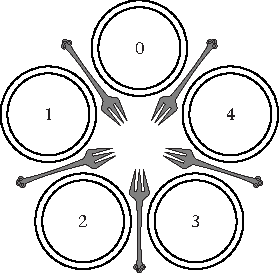
\includegraphics{hail_f0420}}
%\centerline{\epsfbox{dining.eps}}
\caption{Five philosophers, numbered 0 through 4, have places around a
  circular dining table.  There is a fork between each pair of
  adjacent places.  When each philosopher tries to pick up two forks,
  one at a time,
  deadlock can result.}
\label{dining-figure}
\end{figure}
Apparently
Dijkstra was not concerned with communicable diseases such as
mononucleosis, because he thought it was OK for the philosophers
seated to the left and right of a particular fork to share it.
Instead, he was concerned with the possibility of deadlock.  If all five philosophers start by
picking up their respective left-hand forks and then wait for their right-hand forks to become available, they wind up deadlocked.
In
Exploration Project~\ref{dining-philosophers-project}, you can try out
a computer simulation of the dining philosophers.  In that same Exploration
Project, you can also apply the deadlock prevention approach described
in Section~\ref{deadlock-prevention-section} to the dining
philosophers problem.

Deadlocks are usually quite rare even if no special attempt is made
to prevent them, because most locks are not held very long.  Thus,
the window of opportunity for deadlocking is quite narrow, and, like
races, the timing must be exactly wrong.  For a very noncritical system,
one might choose to ignore the possibility of deadlocks.  Even if the
system needs the occasional reboot due to deadlocking, other
malfunctions will probably be more common.  Nonetheless, you should
learn some options for dealing with deadlocks, both because some
systems are critical and because ignoring a known problem is
unprofessional.  In Sections \ref{deadlock-prevention-section} through
\ref{immediate-dd-section}, I explain three of the
most practical ways to address the threat of deadlocks.

\subsection{Deadlock Prevention Through Resource Ordering}\label{deadlock-prevention-section}

The ideal way to cope with deadlocks is to prevent them from
happening.  One very practical technique for deadlock prevention can
be illustrated through the example of transferring money between two bank accounts.
Each of the two accounts is stored somewhere in the computer's
memory, which can be specified through a numerical address.  I will
use the notation \verb|min(account1, account2)| to mean whichever of
the two account objects occurs at the lower address (earlier in
memory). Similarly, I will use \verb|max(account1, account2)| to mean
whichever occurs at the higher address.  I can use this ordering on
the accounts (or any other ordering, such as by account number) to
make a deadlock-free transfer procedure:
\begin{verbatim}
to transfer amount from sourceAccount to destinationAccount:
  lock min(sourceAccount, destinationAccount).mutex
  lock max(sourceAccount, destinationAccount).mutex
  sourceAccount.balance = sourceAccount.balance - amount
  destinationAccount.balance = destinationAccount.balance + amount
  unlock sourceAccount.mutex
  unlock destinationAccount.mutex
\end{verbatim}

Now if I try transferring money to you, and you try transferring money
to me, we will both lock the two accounts' mutexes in the same order.
No deadlock is possible; one transfer will run to completion, and then
the other.

The same technique can be used whenever all the mutexes (or other
resources) to be acquired are known in advance.  Each thread should
acquire the resources it needs in an agreed-upon order, such as by
increasing memory address.  No matter how many threads and resources
are involved, no deadlock can occur.

As one further example of this technique, you can look at some code
from the Linux kernel.  Recall from Chapter~\ref{scheduling-chapter} that the scheduler keeps the run queue,
which holds runnable
threads, in a data structure.  In the kernel
source code, this structure is
known as an \texttt{rq}.  Each processor in a multiprocessor system has
its own \texttt{rq}.  When the scheduler moves a thread from one processor's
\texttt{rq} to another's, it needs to lock both \texttt{rq}s.
Figure~\ref{double_rq_lock} shows the code to
do this.  Note that this
procedure uses the deadlock prevention technique with one refinement:
it also tests for the special case that the two runqueues are
in fact one and the same.
\begin{figure}
%examplesource: linux-2.6.39/kernel/sched.c
%exampleedit: indentation increment reduced to fit margin
\begin{verbatim}
static void double_rq_lock(struct rq *rq1, struct rq *rq2)
  __acquires(rq1->lock)
  __acquires(rq2->lock)
{
  BUG_ON(!irqs_disabled());
  if (rq1 == rq2) {
    raw_spin_lock(&rq1->lock);
    __acquire(rq2->lock);   /* Fake it out ;) */
  } else {
    if (rq1 < rq2) {
      raw_spin_lock(&rq1->lock);
      raw_spin_lock_nested(&rq2->lock, SINGLE_DEPTH_NESTING);
    } else {
      raw_spin_lock(&rq2->lock);
      raw_spin_lock_nested(&rq1->lock, SINGLE_DEPTH_NESTING);
    }
  }
}
\end{verbatim}
\caption{The Linux scheduler uses deadlock prevention when locking two
run queues.}
\label{double_rq_lock}
\end{figure}

Deadlock prevention is not always possible.  In particular, the
ordering technique I showed cannot be used if the mutexes that need
locking only become apparent one by one as the computation proceeds,
such as when following a linked list or other pointer-based
data structure.  Thus, you need to consider coping with deadlocks,
rather than only preventing them.

\subsection{Ex Post Facto Deadlock Detection}\label{post-facto-dd-section}
\index{deadlock detection}
In order to diagnose deadlocks, you need some information about who is
waiting for whom.  Suppose that each mutex records not just whether it
is locked or unlocked, but also which thread it is held by, if any.
(This information may be useful for unrelated purposes as well, such
as implementing recursive or error-checking mutexes.)  Additionally,
when a thread is unable to immediately acquire a mutex and is put
into a waiting state, you can record which mutex it is waiting for.
With this information, you can construct a \vocab{resource allocation graph}.
Figure~\ref{resource-allocation-graph} shows an example graph for
Section~\ref{deadlock-problem-section}'s sample deadlock between bank account transfers.
Squares are threads and circles are mutexes.  The arrows show which
mutex each thread is waiting to acquire and which thread each mutex
is currently held by.
Because the graph has a cycle, it shows that the system is deadlocked.
\begin{figure}
\centerline{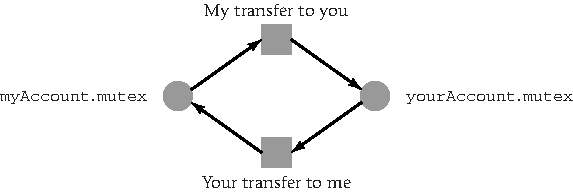
\includegraphics{hail_f0422}}
\iffalse
\centerline{\begin{graph}(294,94)(-43,3)
\graphnodesize{10}
\graphlinecolour{0}
\graphlinewidth{0.5}
\grapharrowlength{5}
\graphnodecolour{0}
\fillednodestrue
\roundnode{myMutex}(50,50)
\roundnode{yourMutex}(150,50)
\squarenode{myTransfer}(100,80)
\squarenode{yourTransfer}(100,20)
\autonodetext{myMutex}[w]{myAccount.mutex}
\autonodetext{yourMutex}[e]{yourAccount.mutex}
\autonodetext{myTransfer}[n]{my transfer to you}
\autonodetext{yourTransfer}[s]{your transfer to me}
\diredge{myTransfer}{yourMutex}
\diredge{yourMutex}{yourTransfer}
\diredge{yourTransfer}{myMutex}
\diredge{myMutex}{myTransfer}
\end{graph}}
\fi
\caption{The cycle in this resource allocation graph indicates a
  deadlock.  Each square represents a thread and each circle a mutex.
  An arrow from a square to a circle shows a thread waiting for a
  mutex, whereas an arrow from a circle to a square shows a mutex
  being held by a thread.}
\label{resource-allocation-graph}
\end{figure}

A system can test for deadlocks periodically or when a thread has
waited an unreasonably long time for a lock.  In order to test for a
deadlock, the system uses a standard graph algorithm to check whether
the resource allocation graph contains a cycle. With the sort of
mutexes described in this book, each mutex can be held by at most
one thread and each thread is waiting for at most one mutex, so no
vertex in the graph has an out-degree greater than 1.  This allows a
somewhat simpler graph search than in a fully-general directed graph.

Once a deadlock is detected, a painful action is needed in order to
recover: one of the deadlocked threads must be forcibly terminated, or
at least rolled back to an earlier state, so as to free up the
mutexes it holds.  In a general computing environment, where threads
have no clean way to be rolled back, this is bit akin to freeing
yourself from a bear trap by cutting off your leg.  For this reason,
ex post facto deadlock detection is not common in general-purpose
operating systems.

One environment in which ex post facto deadlock detection and recovery
works cleanly is database systems, with their support for atomic
transactions.  I will explain atomic transactions in Chapter~\ref{transactions-chapter};
for now, you need only understand that a transaction can
cleanly be rolled back, such that all the updates it made to the
database are undone.  Because this infrastructure is available,
database systems commonly include deadlock detection.  When a deadlock
is detected, one of the transactions fails and can be rolled back,
undoing all its effects and releasing all its locks.  This breaks the
deadlock and allows the remaining transactions to complete.  The
rolled-back transaction can then be restarted.

Figure~\ref{oracle-deadlock} shows an example scenario of deadlock
detection taken from the Oracle database system.
This transcript shows the time interleaving of two
different sessions connected to the same database.  One session is
shown at the left margin, while the other session is shown indented
four spaces.  Command lines start with the system's prompt,
\texttt{SQL>}, and then contain a command typed by the user.  Each
command line is broken on to a second line, to fit the width of this
book's pages.
Explanatory comments start with \texttt{-{}-}.  All other lines are
output.
In Chapter~\ref{transactions-chapter} I will show the recovery from this particular
deadlock as part of my explanation of transactions.
\begin{figure}
%Note that I've taken liberties with when the SQL> prompt is displayed,
%always putting it where the command is being entered, rather than when
%it was actually displayed (eariler).  I've also had to break lines.
\begin{verbatim}
SQL> update accounts set balance = balance - 100
                     where account_number = 1;

1 row updated.

    SQL> update accounts set balance = balance - 250
                         where account_number = 2;

    1 row updated.

SQL> update accounts set balance = balance + 100 
                         where account_number = 2;
-- note no response, for now this SQL session is hanging

    SQL> update accounts set balance = balance + 250 
                         where account_number = 1;
    -- this session hangs, but in the other SQL session we get
    -- the following error message:

update accounts set balance = balance + 100 
                where account_number = 2
       *
ERROR at line 1:
ORA-00060: deadlock detected while waiting for resource 
\end{verbatim}
\caption{The Oracle database
  system detects a deadlock between two sessions connected to the same
  database.  One session, shown at the left margin, is transferring \$100
  from account 1 to account 2.  The other session, shown indented, is
  transferring \$250 from account 2 to account 1.  Each update statement
  locks the account being updated.  Therefore, each session hangs when it
  tries locking the account that the other session has previously locked.}
\label{oracle-deadlock}
\end{figure}

\subsection{Immediate Deadlock Detection}\label{immediate-dd-section}

The two approaches to deadlocks presented thus far are aimed
at the times before and after the moment when deadlock occurs.  One
arranges that the prerequisite circumstances leading to deadlock do
not occur, while the other notices that deadlock already has occurred,
so that the mess can be cleaned up.  Now I will turn to a third
alternative: intervening at the very moment when the system would
otherwise deadlock.  Because this intervention requires techniques similar to those discussed in Section~\ref{post-facto-dd-section}, this technique is conventionally known
as a form of deadlock detection rather than deadlock prevention, even
though from a literal perspective the deadlock is prevented from
happening.

As long as no deadlock is ever allowed to occur, the resource
allocation graph will remain acyclic, that is, free of cycles.  Each time a thread tries to
lock a mutex, the system can act as follows:
\begin{itemize}
\item
If the mutex is unlocked, lock it and add an edge from the mutex to
the thread, so as to indicate which thread now holds the lock.
\item
If the mutex is locked, follow the chain of edges from it until that
chain dead ends.  (It must, because the graph is acyclic.)  Is the end
of the chain the same as the thread trying to lock the mutex?
\begin{itemize}
\item
If not, add an edge showing that the thread is waiting for the mutex,
and put the thread into a waiting state.
\item
If the end of the chain is the same thread, adding the extra edge would complete a cycle, as shown in
Figure~\ref{idd-rg-figure}.
\begin{figure}
\centerline{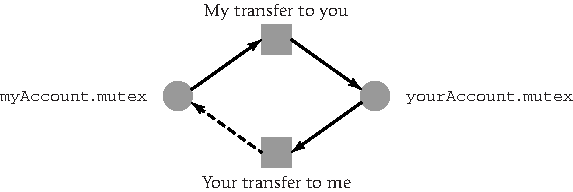
\includegraphics{hail_f0424}}
\iffalse
\centerline{\begin{graph}(294,94)(-43,3)
\graphnodesize{10}
\graphlinecolour{0}
\graphlinewidth{0.5}
\grapharrowlength{5}
\graphnodecolour{0}
\fillednodestrue
\roundnode{myMutex}(50,50)
\roundnode{yourMutex}(150,50)
\squarenode{myTransfer}(100,80)
\squarenode{yourTransfer}(100,20)
\autonodetext{myMutex}[w]{myAccount.mutex}
\autonodetext{yourMutex}[e]{yourAccount.mutex}
\autonodetext{myTransfer}[n]{my transfer to you}
\autonodetext{yourTransfer}[s]{your transfer to me}
\diredge{myTransfer}{yourMutex}
\diredge{yourMutex}{yourTransfer}
\diredge{yourTransfer}{myMutex}[\graphlinedash{1 2}]
\diredge{myMutex}{myTransfer}
\end{graph}}
\fi
\caption{In this resource graph, the solid arrows indicate that my
  transfer holds {\tt myAccount.mutex}, your transfer holds {\tt
  yourAccount.mutex}, and my transfer is waiting for {\tt
  yourAccount.mutex}.  The dashed arrow indicates a request currently
  being made by your transfer to lock {\tt myAccount.mutex}. If this
  dashed arrow is added, a
  cycle is completed, indicating a deadlock.  Therefore, the request
  will fail rather than enter a state of waiting.}
\label{idd-rg-figure}
\end{figure}
Therefore, don't add the edge, and don't put
the thread into a waiting state.  Instead, return an error code from the
lock request (or throw an exception), indicating that the mutex could
not be locked because a deadlock would have resulted.
\end{itemize}
\end{itemize}

Notice that the graph search here is somewhat simpler than in
ex post facto deadlock detection, because the graph is kept acyclic.
Nonetheless, the basic idea is the same as deadlock detection, just
done proactively rather than after the fact.  As with any deadlock
detection, some form of roll-back is needed; the application program
that tried to lock the mutex must respond to the news that its request
could not be granted.  The application program must not simply try
again to acquire the same mutex, because it will repeatedly get the
same error code.  Instead, the program must release the locks it
currently holds and then restart from the beginning.  The chance of
needing to repeat this response can be reduced by sleeping briefly
after releasing the locks and before restarting.

Designing an application program to correctly handle immediate
deadlock detection can be challenging.  The difficulty is that before
the program releases its existing locks, it should restore the objects
those locks were protecting to a consistent state.  One case in which
immediate deadlock detection can be used reasonably easily is in a
program that acquires all its locks before it modifies any objects.

One example of immediate deadlock detection is in
Linux and Mac OS~X, for the readers/writers locks placed on files using
\index{fcntl@\verb"|fcntl"|}\verb|fcntl|.  If a lock request would complete a cycle, the
\verb|fcntl| procedure returns the error code \index{EDEADLK@\verb"|EDEADLK"|}\verb|EDEADLK|.  However, this
deadlock detection is not a mandatory part of the POSIX specification
for \verb|fcntl|.

\section{The Interaction of Synchronization with Scheduling}\label{synchronization-and-scheduling-section}

Recall that the scheduler controls which runnable thread runs on each processor, and
synchronization actions performed by the running thread control which
threads are runnable.  Therefore, synchronization and scheduling interact with one another.
Two forms of interaction, known as priority inversion and the convoy
phenomenon, are particularly interesting.  Said another way, they can
cause lots of grief.  Each can subvert the prioritization of threads,
and the convoy phenomenon can also greatly increase the context
switching rate and hence decrease system throughput.
For simplicity, each is presented here under the assumption of a single-processor system.

\subsection{Priority Inversion}

When a priority-based scheduler is used, a high-priority thread should
not have to wait while a low-priority thread runs.  If threads of
different priority levels share mutexes or other blocking synchronization
primitives, some minor violations of priority ordering are
inevitable.  For example, consider the following sequence of events
involving two threads (high-priority and low-priority) that share a
single mutex:
\begin{enumerate}
\item
The high-priority thread goes into the waiting state, waiting for an
I/O request to complete.
\item
The low-priority thread runs and acquires the mutex.
\item
The I/O request completes, making the high-priority thread runnable
again.  It preempts the low-priority thread and starts running.
\item
The high-priority thread tries to acquire the mutex.  Because the mutex
is locked, the high-priority thread is forced to wait.
\item
The low-priority thread resumes running.
\end{enumerate}
At this point, a high-priority thread is waiting while a low-priority
thread runs.  However, this temporary violation of priority ordering
is not a big deal, because programmers generally ensure that no thread
holds a mutex for very long.  As such, the low-priority thread will
soon release the mutex and allow the high-priority thread to run.

However, another, more insidious problem can lead to longer-term
violation of priority order (that is, \foldvocab{priority}{inversion}).  Suppose
there are three threads, of low, medium, and high priority.  Consider this
sequence of events:
\begin{enumerate}
\item
The high- and medium-priority threads both go into the waiting state,
each waiting for an I/O request to complete.
\item
The low-priority thread runs and acquires the mutex.
\item
The two I/O requests complete, making the high- and medium-priority
threads runnable.  The high-priority thread preempts the low-priority
thread and starts running.
\item
The high-priority thread tries to acquire the mutex.  Because the mutex
is locked, the high-priority thread is forced to wait.
\item
At this point, the medium-priority thread has the highest priority of
those that are runnable.  Therefore it runs.
\end{enumerate}

In this situation, the medium-priority thread is running and
indirectly keeping the high-priority thread from running.  (The
medium-priority thread is blocking the low-priority thread by virtue
of their relative priorities.  The low-priority thread is blocking the
high-priority thread by holding the mutex.)  The medium-priority
thread could run a long time.  In fact, a whole succession of
medium-priority threads with overlapping lifetimes could come and
go, and the high-priority thread would wait the whole time despite its
higher priority.  Thus, the priority inversion could continue for an arbitrarily long time.

One ``solution'' to the priority inversion problem is to avoid
fixed-priority scheduling.  Over time, a decay usage scheduler will
naturally lower the priority of the medium-priority thread that is
running.  Eventually it will drop below the low-priority thread, which
will then run
and free the mutex, allowing the high-priority thread to run.
However, a succession of medium-priority threads, none of which runs
for very long, could still hold up the high-priority thread
arbitrarily long.  Therefore, Microsoft Windows responds to priority
inversion by periodically boosting the priority of waiting low-priority processes.

This first ``solution'' has two shortcomings.  First, it may be sluggish in
responding to a priority inversion.  Second, fixed-priority scheduling
is desirable in some applications, such as real-time systems.
Therefore, a genuine solution to the priority inversion
problem is needed---one that makes the problem go away, rather than just
limiting the duration of its effect.  The genuine solution is
\foldvocab{priority}{inheritance}.

Priority inheritance is a simple idea: any thread that is waiting for
a mutex temporarily ``lends'' its priority to the thread that holds
the mutex.  A thread that holds mutexes runs with the highest priority
among its own priority and those priorities it has been lent by threads waiting for the
mutexes.  In the example with three threads, priority inheritance will allow the low-priority thread that
holds the mutex to run as though it were high-priority until it
unlocks the mutex.  Thus, the truly high-priority thread will get to
run as soon as possible, and the medium-priority thread will have to
wait.

Notice that the high-priority thread has a very selfish motive for
letting the low-priority thread use its priority: it wants to get the
low-priority thread out of its way.  The same principle can be applied
with other forms of scheduling than priority scheduling.  By analogy
with priority inheritance, one can have \foldvocab{deadline}{inheritance} (for
Earliest Deadline First scheduling) or even a lending of processor
allocation shares (for proportional-share scheduling).

\subsection{The Convoy Phenomenon}\label{convoy-section}

I have remarked repeatedly that well-designed programs do not
normally hold any mutex for very long; thus, attempts to lock a mutex
do not normally encounter contention.  This is important because
locking a mutex with contention is much more expensive.  In
particular, the big cost of a request to lock an already-locked mutex
is context switching, with the attendant loss of cache performance.
Unfortunately, one particularly nasty interaction between scheduling
and synchronization, known as the \vocab{convoy phenomenon}, can sometimes
cause a heavily used mutex to be perpetually contended, causing a
large performance loss.  Moreover, the convoy phenomenon can subvert
scheduling policies, such as the assignment of priorities. In this
subsection, I will explain the convoy phenomenon and examine some
solutions.

Suppose a system has some very central data structure, protected by a
mutex, which each thread operates on fairly frequently.  Each time a
thread operates on the structure, the thread locks the mutex before
and unlocks it after.  Each operation is kept as short as possible.
Because they are frequent, however, the mutex spends some appreciable
fraction of the time locked, perhaps 5 percent.

The scheduler may at any point preempt a thread.  For example, the
thread may have consumed its allocated time slice.  In the example
situation where the mutex is locked 5 percent of the time, it would not be
very surprising if after a while, a thread were preempted while it
held the mutex.  When this happens, the programmer who wrote that
thread loses all control over how long it holds the mutex locked.
Even if the thread was going to unlock the mutex in its very next
instruction, it may not get the opportunity to execute that next
instruction for some time to come.  If the processor is dividing its
time among $N$ runnable threads of the same priority level, the thread
holding the mutex will presumably not run again for at least $N$ times
the context-switching time, even if the other threads all immediately
block.

In this situation, a popular mutex is held for a long time.
Meanwhile, other threads are running.  Because the mutex is a popular
one, the chances are good those other threads will try to acquire it.
Because the mutex is locked, all the threads that try to acquire the mutex will be queued on
its wait queue.  This queue of threads is the \vocab{convoy}, named by
analogy with the unintentional convoy of vehicles that develops behind
one slow vehicle on a road with no passing lane.  As you will see,
this convoy spells trouble.

Eventually the scheduler will give a new time slice to the thread that
holds the mutex.  Because of that thread's design, it will quickly
unlock the mutex.  When that happens, ownership of the mutex is passed
to the first thread in the wait queue, and that thread is made
runnable.  The thread that unlocked the mutex continues to run,
however.  Because it was just recently given a new time slice, one might
expect it to run a long time.  However, it probably won't, because
before too terribly long, it will try to reacquire the popular mutex
and find it locked.  (``Darn,'' it might say, ``I shouldn't have given
that mutex away to the first of the waiters.  Here I am needing it
again myself.'')  Thus, the thread takes its place at the back of the
convoy, queued up for the mutex.

At this point, the new holder of the mutex gets to run, but it too
gives away the mutex, and hence is unlikely to run a full time slice
before it has to queue back up.  This continues, with each thread in
turn moving from the front of the mutex queue through a brief period
of execution and back to the rear of the queue.  There may be slight
changes in the makeup of the convoy---a thread may stop waiting on the
popular mutex, or a new thread may join---but seen in the aggregate,
the convoy can persist for a very long time.

This situation causes two problems.  First, the context switching rate
goes way up; instead of one context switch per time slice, there is now
one context switch per attempt to acquire the popular mutex.  The
overhead of all those context switches will drive down the system
throughput.  Second, the scheduler's policy for choosing which thread
to run is subverted.  For example, in a priority scheduler, the
priorities will not govern how the threads run.  The reason for this
is simple: the scheduler can choose only among the runnable threads,
but with the convoy phenomenon, there will only be one runnable
thread; all the others will be queued up for the mutex.

When I described mutexes, I said that each mutex contains a wait
queue---a list
of waiting threads.  I implied that this list is maintained in a
first-in first-out (FIFO) basis, that is, as a true queue.  If so, then the
convoy threads will essentially be scheduled in a FIFO round-robin,
independent of the scheduler policy (for example, priorities), because the
threads are dispatched from the mutex queue rather than the
scheduler's run queue.

This loss of prioritization can be avoided by handling
the mutex's wait queue in priority order the same way as
the run queue, rather than FIFO.  When a mutex is
unlocked with several threads waiting, ownership of the mutex could be
passed not to the thread that waited the longest, but rather to the
one with the highest priority.

Changing which one thread is moved from the mutex's waiters list to
become runnable does not solve the throughput problem, however.  The
running thread is still going to have the experience I
anthropomorphized as ``Darn, I shouldn't have given that mutex away.''
The context switching rate will still be one switch per lock
acquisition.  The convoy may reorder itself, but it will not
dissipate.

Therefore, stronger medicine is needed for popular mutexes.  Instead
of the mutexes I showed in Figures \ref{lock-pseudo-code} and
\ref{unlock-pseudo-code} on page~\pageref{lock-pseudo-code}, you can
use the version shown in Figure~\ref{convoy-pseudo-code}.
\begin{figure}
\begin{verbatim}
to lock mutex:
  repeat
    lock mutex.spinlock (in cache-conscious fashion)
    if mutex.state = 1 then
      let mutex.state = 0
      unlock mutex.spinlock
      let succesful = true
    else
      add current thread to mutex.waiters
      remove current thread from runnable threads
      unlock mutex.spinlock
      yield to a runnable thread
      let successful = false
  until successful

to unlock mutex:
  lock mutex.spinlock (in cache-conscious fashion)
  let mutex.state = 1
  move all threads from mutex.waiters to runnable
  unlock mutex.spinlock
\end{verbatim}
\caption{To protect against convoys, the unlock operation sets the
  mutex's state to unlocked and makes all waiting threads runnable.
  Each awoken thread loops back to trying to lock the mutex.  This
  contrasts with the prior version of mutexes, in which one thread
  was awoken with the mutex left in its locked state.}
\label{convoy-pseudo-code}
\end{figure}

When a popular mutex is unlocked, {\em all} waiting threads are made
runnable and moved from the waiters list to the runnable threads list.
However, ownership of the mutex is not transferred to any of them.
Instead, the mutex is left in the unlocked state, with \verb|mutex.state| equal to 1.  That way, the
running thread will not have to say ``Darn.''  It can simply relock
the mutex; over the course of its time slice, it may lock and unlock
the mutex repeatedly, all without context switching.

Because the mutex is only held 5 percent of the time, the
mutex will probably not be held when the thread eventually blocks for
some other reason (such as a time slice expiration).  At that point, the
scheduler will select one of the woken threads to run.  Note that this
will naturally follow the normal scheduling policy, such as priority
order.

The woken thread selected to run next did not have the mutex ownership
directly transferred to it.  Therefore, it will need to loop back to
the beginning of the mutex acquisition code, as will each thread in
turn when it is scheduled.  However, most of the time the threads will
find the mutex unlocked, so this won't be expensive.  Also, because each
thread will be able to run for a normal period without context-switching overhead per lock request, the convoy will dissipate.

The POSIX standard API for mutexes requires that one or the other of
the two prioritization-preserving approaches be taken.  At a minimum, if ownership of a
mutex is directly transferred to a waiting thread, that waiting thread
must be selected based on the normal scheduling policy rather than
FIFO.  Alternatively, a POSIX-compliant mutex implementation can
simply dump all the waiting threads back into the scheduler and let it
sort them out, as in Figure~\ref{convoy-pseudo-code}.

\section{Nonblocking Synchronization}\label{nonblocking-synchronization-section}\foldindex{nonblocking}{synchronization}
In order to introduce nonblocking synchronization with a concrete example, let's return
to the \texttt{TicketVendor} class shown in Figure~\ref{TicketVendor} on page~\pageref{TicketVendor}.
In that example, whenever a thread is selling a ticket, it temporarily blocks any other
thread from accessing the same \texttt{TicketVendor}.  That ensures that the \texttt{seatsRemaining}
and \texttt{cashOnHand} are kept consistent with each other, as well as preventing two threads from both
selling the last available ticket.  The downside is that if the scheduler ever preempts a thread
while it holds the \texttt{TicketVendor}'s lock, all other threads that want to use the same \texttt{TicketVendor} remain blocked until the first thread runs again, which might be arbitrarily far in the future.  Meanwhile, no progress is made on vending tickets or even on conducting an audit.  This kind of blocking underlies both priority inversion and the convoy phenomenon and if extended through a cyclic chain of objects can even lead to deadlock.  Even absent those problems, it hurts performance.  What's needed is a lock-free \texttt{TicketVendor} that manages to avoid race bugs without this kind of unbounded blocking.

Recall that the spinlocks introduced in Section~\ref{mutex-mechanisms-section} use atomic exchange instructions.  A thread that succeeds in changing a lock from the unlocked state to the locked state is guaranteed that no other thread did the same.  The successful thread is thereby granted permission to make progress, for example by vending a ticket. However, actually making progress and then releasing the lock are separate actions, not part of the atomic exchange.  As such, they might be delayed.  A nonblocking version of the \texttt{TicketVendor} requires a more powerful atomic instruction that can package the actual updating of the \texttt{TicketVendor} with the obtaining of permission.

The \index{compare-and-set}compare-and-set instruction meets this need by doing the following two things atomically:
\begin{enumerate}
\item The instruction determines whether a variable contains a specified value and reports the answer.
\item The instruction sets the variable to a new value, but only if the answer to the preceding question was ``yes.''
\end{enumerate}
Some variant of this instruction is provided by all contemporary processors.  Above the hardware
level, it is also part of the Java API through the classes included in the \texttt{java.util.concurrent.atomic} package.
Figures \ref{nonblocking-TicketVendor1} and \ref{nonblocking-TicketVendor2} show a nonblocking version of the \texttt{TicketVendor} class that uses one
of these classes, \texttt{AtomicReference}.
\begin{figure}
\begin{verbatim}
import java.util.concurrent.atomic.AtomicReference;

public class LockFreeTicketVendor { 
    
  private static class State {
    private int seatsRemaining, cashOnHand;
    
    public State(int seatsRemaining, int cashOnHand) {
      this.seatsRemaining = seatsRemaining;
      this.cashOnHand = cashOnHand;
    }

    public int getSeatsRemaining(){return seatsRemaining;}
    public int getCashOnHand(){return cashOnHand;}
  }

  private AtomicReference<State> state;
  private int startingSeats, startingCash;

  public LockFreeTicketVendor(int startingSeats,
                              int startingCash) {
    this.startingSeats = startingSeats;
    this.startingCash = startingCash;
    this.state = new AtomicReference<State>
      (new State(startingSeats, startingCash));
  }

  // See next figure for sellTicket and audit methods.

  // Other details also remain to be filled in.
}
\end{verbatim}
\caption{This lock-free ticket vendor uses nonblocking synchronization.
Notice that rather than directly storing the \texttt{seatsRemaining}
and \texttt{cashOnHand}, it stores an \texttt{AtomicReference} to a
\texttt{State} object that packages these two variables together,
allowing them to be kept consistent without locking.
The next figure shows how this \texttt{AtomicReference} is used.}\label{nonblocking-TicketVendor1}
\end{figure}
\begin{figure}
\begin{verbatim}    
  public void sellTicket(){
    while(true){
      State snapshot = state.get();
      int seatsRemaining = snapshot.getSeatsRemaining();
      int cashOnHand = snapshot.getCashOnHand();
      if(seatsRemaining > 0){
        State next = new State(seatsRemaining - 1,
                               cashOnHand + PRICE);
        if(state.compareAndSet(snapshot, next)){
          dispenseTicket();
          return;
        }
      } else {
        displaySorrySoldOut();
        return;
      }
    }
  }
    
  public void audit() { 
    State snapshot = state.get();
    int seatsRemaining = snapshot.getSeatsRemaining();
    int cashOnHand = snapshot.getCashOnHand();
    // check seatsRemaining, cashOnHand
  } 
\end{verbatim}
\caption{These methods from the previous figure's lock-free ticket vendor show how the \texttt{AtomicReference} supports nonblocking synchronization.  A consistent snapshot can be taken of the current state, and the state is only set to an updated version
 (and a ticket dispensed) if the snapshot remains valid.}
\label{nonblocking-TicketVendor2}
\end{figure}

In this example, the \texttt{sellTicket} method attempts to make progress using the following method invocation:
\begin{verbatim}
state.compareAndSet(snapshot, next)
\end{verbatim}
If the state still matches the earlier snapshot, then no other concurrent thread has snuck in and sold a ticket.
In this case, the state is atomically updated and the method returns \texttt{true}, at which point a ticket can
safely be dispensed.  On the other hand, if the method returns \texttt{false}, then the enclosing \texttt{while} loop
will retry the whole process, starting with getting a new snapshot of the state.  You can explore this behavior in Programming Project~\ref{nonblocking-TicketVendor-project}.

The \foldvocab{lock-free}{synchronization} illustrated by this example ensures that
no thread will ever be blocked waiting for a lock held by some other
thread.  In particular, no matter how long the scheduler chooses to
delay execution of any thread, other threads can continue making
progress.  However, there is still one way a thread might end up
running arbitrarily long without making progress, which is if over and
over again, other threads slip in and update the state.  In a case
like that, the system as a whole continues to make progress---tickets
continue being sold---but one particular thread keeps retrying.
Stronger forms of nonblocking synchronization, known as ``\foldvocab{wait-free}{synchronization},'' guarantee that each individual thread makes
progress.  However, wait-free synchronization is considerably more
complex than the style of lock-free synchronization shown here
and hence is rarely used in practice.

Similar techniques can be used to create lock-free data structures
that allow multiple threads to carry out operations concurrently, to
the maximum extent possible. For example, if a queue is going to
deliver data in a well-defined order, dequeue operations need to be
processed sequentially, but there is no reason additional data can't
be enqueued onto an already non-empty queue at the same time as
earlier data is dequeued. Such data structures aren't easy to design
and program; achieving high performance and concurrency without
introducing bugs is quite challenging.  However, concurrent data
structures can be programmed once by experts and then used as building
blocks.  Concurrent queues in particular can be used in frameworks
that queue up tasks to be processed by a pool of threads;
one example is Apple's Grand Central Dispatch framework.

\section{Security and Synchronization}\label{synchronization-and-security-section}

A system can be insecure for two reasons: either because its security
policies are not well designed, or because some bug in the code
enforcing those policies allows the enforcement to be bypassed.  For
example, you saw in Chapter~\ref{scheduling-chapter} that a denial of service
attack can be mounted by setting some other user's thread to a very
low priority.  I remarked that as a result, operating systems only
allow a thread's priority to be changed by its owner.  Had this issue
been overlooked, the system would be insecure due to an inadequate
policy.  However, the system may still be insecure if clever programmers
can find a way to bypass this restriction using some low-level bug in
the operating system code.

Many security-critical bugs involve synchronization, or more
accurately, the lack of synchronization---the bugs are generally race
conditions resulting from inadequate synchronization.  Four factors
make race conditions worth investigation by someone exploiting a system's weaknesses
(a \vocab{cracker}):
\begin{itemize}
\item
Any programmer of a complicated concurrent system is likely to introduce
race bugs, because concurrency and synchronization are hard to reason
about.
\item
Normal testing of the system is unlikely to have eliminated these bugs,
because the system will still work correctly the vast majority of the
time.
\item
Although the race might almost never occur in normal operation, the
cracker may be able to trigger the race by understanding it and
carefully staging the necessary sequence of events.  Even if the odds
can't be improved beyond one in ten thousand (for example), the
cracker can easily program a computer to loop through the attempt tens
of thousands of times until the lucky timing happens.
\item
Races allow seemingly impossible situations, defeating the system
designer's careful security reasoning.
\end{itemize}

As a hypothetical example, assume that an operating system had a
feature for changing a thread's priority when given a pointer to a
block of memory containing two values: an identifier for the thread to
be changed and the new priority.  Let's call these
\verb|request.thread| and \verb|request.priority|.  Suppose that the
code looked like this:
\begin{verbatim}
if request.thread is owned by the current user then
  set request.thread's priority to request.priority
else      
  return error code for invalid request
\end{verbatim}
Can you see the race?   A cracker could start out with
\verb|request.thread| being a worthless thread he or she owns and then modify
\verb|request.thread| to be the victim thread after the ownership check but
before the priority is set.  If the timing doesn't work out, no great
harm is done, and the cracker can try again.

This particular example is not entirely realistic in a number of
regards, but it does illustrate a particular class of races often
contributing to security vulnerabilities: so-called \vocab{TOCTTOU} races,
an acronym for \vocab{Time Of Check To Time Of Use}.  An operating system
designer would normally guard against this particular TOCTTOU bug by
copying the whole request structure into protected memory before doing
any checking.  However, other TOCTTOU bugs arise with some
regularity.  Often, they are not in the operating system kernel
itself, but rather in a privileged program.

For example, suppose an email delivery program is granted the
privilege of writing into any file, independent of file ownership or
normal protections, so that it can deliver each user's mail into that
user's mail file.  Before delivering mail into a mail file, it will
check that the mail file is a normal file that is really in the expected
location, not an indirect reference (symbolic link) to a file located
elsewhere.  (I will explain symbolic links in Chapter~\ref{persistence-chapter}, when I cover file
systems.  The details are not important here.)  That way, you cannot
trick the mail delivery program into writing into some sensitive file.
Or can you?  Perhaps by changing from a genuine mail file to a
symbolic link at just the right moment, you can exploit a TOCTTOU
vulnerability.  Sun Microsystems had this particular problem with
their mail software in the early 1990s.

\section*{Exercises}
\begin{chapterEnumerate}
\item\label{race-exercise}
As an example of a race condition, I showed how two threads could
each dispense the last remaining ticket by each checking
\verb|seatsRemaining| before either decrements it.  Show a different
sequence of events for that same code, whereby starting with
\verb|seatsRemaining| being 2, two threads each dispense a ticket, but
\verb|seatsRemaining| is left as 1 rather than 0.
\item\label{buggy-lock-pseudo-code-exercise}
In the mutex-locking pseudocode of Figure~\ref{lock-pseudo-code} on
page~\pageref{lock-pseudo-code}, there
are two consecutive steps that remove the current thread from the
runnable threads and then unlock the spinlock.  Because spinlocks should
be held as briefly as possible, we ought to consider whether these
steps could be reversed, as shown in Figure~\ref{buggy-lock-pseudo-code}.  Explain why reversing them would be a bad
idea by giving an example sequence of events where the reversed
version malfunctions.
\begin{figure}
\begin{verbatim}
to lock mutex:
  lock mutex.spinlock (in cache-conscious fashion)
  if mutex.state = 1 then
    let mutex.state = 0
    unlock mutex.spinlock
  else
    add current thread to mutex.waiters
    unlock mutex.spinlock
    remove current thread from runnable threads
    yield to a runnable thread
\end{verbatim}
\caption{This is a buggy version of Figure~\ref{lock-pseudo-code}. Exercise~\ref{buggy-lock-pseudo-code-exercise} asks you to explain what is wrong with it.}
\label{buggy-lock-pseudo-code}
\end{figure}
\item\label{recursive-mutex-exercise}
Show how to change queuing mutexes to correspond with
POSIX's mutex-type \texttt{PTHREAD\_MUTEX\_RECURSIVE}.  You may add additional
components to each mutex beyond the state, waiters, and spinlock.
\item\label{notify-exercise}
Explain why replacing \verb|notifyAll| by \verb|notify| is not safe in
the \verb|Bounded|\linebreak[0]\verb|Buffer| class of Figure~\ref{BoundedBuffer.java} on
page~\pageref{BoundedBuffer.java}.
Give a concrete sequence of events under which
the modified version would misbehave.
\item
A semaphore can be used as a mutex.  Does it correspond with the kind
POSIX calls \texttt{PTHREAD\_MUTEX\_ERROR\_CHECK}, \texttt{PTHREAD\_MUTEX\_NORMAL}, or
\texttt{PTHREAD\_MUTEX\_RECURSIVE}?  Justify your answer.
\item
State licensing rules require a child-care center to have no more than
three infants present for each adult.  You could enforce this rule
using a semaphore to track the remaining capacity, that is, the number of
additional infants that may be accepted.  Each time an infant is about
to enter,
an \verb|acquire| operation is done first, with a \verb|release| when the infant
leaves.  Each time an adult enters, you do three \verb|release| operations,
with three \verb|acquire| operations before the adult may leave.
\begin{enumerate}
\item
Although this system will enforce the state rules, it can create a
problem when two adults try to leave.  Explain what can go wrong, with
a concrete scenario illustrating the problem.
\item
The difficulty you identified in the preceding subproblem can be remedied by using a mutex as well
as the semaphore. Show how.
\item
Alternatively, you could abandon semaphores entirely and use a monitor
with one or more condition variables.  Show how.
\end{enumerate}
\item
I illustrated deadlock detection using a transcript taken from an
Oracle database (Figure~\ref{oracle-deadlock},
page~\pageref{oracle-deadlock}).  From that transcript you can tell
that the locks are at the granularity of one per row, rather
than one per table.
\begin{enumerate}
\item
What is the evidence for this assertion?
\item
Suppose the locking were done per table instead.  Explain why no
deadlock would have ensued.
\item
Even if locking were done per table, deadlock could still happen other
under circumstances.  Give an example.
\end{enumerate}
\item
Suppose you have two kinds of objects: threads and mutexes.  Each
locked mutex contains a reference to the thread that holds it named
\verb|mutex.owner|; if the mutex is unlocked, \verb|mutex.owner| is
\verb|null|.  Similarly, each thread that is blocked waiting for a
mutex contains a reference to the mutex it is waiting for as
\verb|thread.blocker|; if the thread is not waiting for any mutex,
\verb|thread.blocker| is \verb|null|.  Suppose threads also contain a
field, \verb|thread.mark|, which is available for your use and is
initialized to 0.  Further, suppose you have an array of all the
threads in the system as \verb|threads[0]|, \verb|threads[1]|, and so
forth,
up to \verb|threads[threads.length-1]|.  Write a pseudocode algorithm
to test whether the system contains a deadlock.
\item
The main topic of this chapter (synchronization) is so closely related
to the topics of Chapters \ref{threads-chapter} and
\ref{scheduling-chapter} (threads and scheduling) that
an author can hardly describe one without also describing the other
two.  For each of the following pairs of topics, give a brief
explanation of why understanding the first topic in the pair is useful
for gaining a full understanding of the second:
\begin{enumerate}
\item threads, scheduling
\item threads, synchronization
\item scheduling, synchronization
\item scheduling, threads
\item synchronization, scheduling
\item synchronization, threads
\end{enumerate}
\item\label{priority-inversion-exercise}
Suppose a computer with only one processor runs a program that immediately creates three threads, which are assigned high, medium, and low fixed priorities.  (Assume that no other threads are competing for the same processor.)  The threads share access to a single mutex.  Pseudocode for each of the threads is shown in Figure~\ref{priority-inversion-pseudocode}.
\begin{figure}
\begin{verbatim}
High-priority thread:
  sleep 1 second
  lock the mutex
  terminate execution of the whole program

Medium-priority thread:
  sleep 1 second
  run for 10 seconds

Low-priority thread:
  lock the mutex
  sleep for 2 seconds
  unlock the mutex
\end{verbatim}
\caption{These are the three threads referenced by Exercise~\ref{priority-inversion-exercise}.}\label{priority-inversion-pseudocode}
\end{figure}
\begin{enumerate}
\item
Suppose that the mutex does not provide priority inheritance. How soon would you expect the program to terminate? Why?
\item
Suppose that the mutex provides priority inheritance.  How soon would you expect the program to terminate?  Why?
\end{enumerate}
Programming Project~\ref{priority-inversion-project} gives you the opportunity to experimentally confirm your answers.
\item
Suppose the first three lines of the \texttt{audit} method in Figure~\ref{nonblocking-TicketVendor2} on page~\pageref{nonblocking-TicketVendor2} were replaced by the following two lines:
\begin{verbatim}
    int seatsRemaining = state.get().getSeatsRemaining();
    int cashOnHand = state.get().getCashOnHand();
\end{verbatim}
Explain why this would be a bug.
\end{chapterEnumerate}

\section*{Programming Projects}
\begin{chapterEnumerate}
\item\label{blocking-TicketVendor-project}
Flesh out the \verb|TicketVendor| class from Figure~\ref{TicketVendor} on
page~\pageref{TicketVendor}
using Figure~\ref{tickets-pthreads-code} on page~\pageref{tickets-pthreads-code} for guidance.
Add a simple test program that uses a
\verb|TicketVendor| from multiple threads.  Temporarily remove the
\verb|synchronized| keywords and demonstrate race conditions by
inserting calls to the \verb|Thread.sleep| method at appropriate
points, so that incredibly lucky timing is not necessary.  You should
set up one demonstration for each race previously considered: two threads
selling the last seat, two threads selling seats but the count only
going down by 1, and an audit midtransaction.  Now reinsert the
\verb|synchronized| keyword and show that the race bugs have been
resolved, even with the \verb|sleep|s in place.
\item
Demonstrate races and mutual exclusion as in the previous project,
but using a C program with POSIX threads and mutexes.  Alternatively, use some
other programming language of your choice, with its support for
concurrency and mutual exclusion.
\item\label{simulator-synchronization-project}
Choose some simplified version of a real-world process that evolves
over time, such as a bouncing ball, an investment with compound
interest, or populations of predator and prey.  Write a program with
two threads.  One thread should simulate the process you chose as time
passes, possibly with some suitable scaling such as 1 second of
simulator time per year of simulated time.  The other thread should
provide a user interface through which the user can modify the
parameters of the ongoing simulation and can also pause and resume the
simulation.  Be sure to properly synchronize the two threads.  Java
would be an appropriate language for this project, but you could also
use some other language with support for concurrency, synchronization,
and user interfaces.
\item
This project is identical to the previous one, except that instead of
building a simulator for a real-world process, you should build a game
of the kind where action continues whether or not the user makes a
move.
\item\label{bounded-buffer-test-project}
Write a test program in Java for the \verb|BoundedBuffer| class of
Figure~\ref{BoundedBuffer.java} on page~\pageref{BoundedBuffer.java}.
\item\label{conditional-notifyAll-project}
Modify the \verb|BoundedBuffer| class of Figure~\ref{BoundedBuffer.java}
(page~\pageref{BoundedBuffer.java}) to call \verb|notifyAll| only when
inserting into an empty buffer or retrieving from a full buffer.  Test
that it still works.
\item\label{bb-two-condvars-project}
Rewrite the \verb|BoundedBuffer| class of Figure~\ref{BoundedBuffer.java} 
(page~\pageref{BoundedBuffer.java}) in C or C$++$ using the POSIX
API.  Use two condition variables, one for availability of space and
one for availability of data.
\item\label{rw-project}
Define a Java class for readers/writers locks, analogous to the
\verb|Bounded|\linebreak[0]\verb|Buffer| class of Figure~\ref{BoundedBuffer.java}
(page~\pageref{BoundedBuffer.java}).  Allow additional readers to
acquire a reader-held lock even if writers are waiting. As an
alternative to Java, you may use another programming language with
support for mutexes and condition variables.
\item
Modify your readers/writers locks from the prior project so no
additional readers may acquire a reader-held lock if writers are
waiting.
\item
\label{rwlock-with-upgrade-exercise}
Modify your readers/writers locks from either of the prior two projects
to support an additional operation that a reader can use to upgrade its
status to writer.  (This is similar to dropping the read lock and
acquiring a write lock, except that it is atomic: no other writer can
sneak in and acquire the lock before the upgrading reader does.)  What
happens if two threads both hold the lock as readers, and each tries
upgrading to become a writer?  What do you think a good response would
be to that situation?
\item\label{barrier-project}
Define a Java class for barriers, analogous to the
\verb|BoundedBuffer| class of Figure~\ref{BoundedBuffer.java}
(page~\pageref{BoundedBuffer.java}).  Alternatively, use another programming
language, with support for mutexes and condition variables.
\item\label{semaphore-project}
Define a Java class, \texttt{Semaphore}, such that
you can remove the \texttt{import} line from
Figure~\ref{SemaphoreBoundedBuffer.java} on
page~\pageref{SemaphoreBoundedBuffer.java}
and have that \texttt{BoundedBuffer} class still work.
\item\label{semaphore-array-bb-project}
Rewrite the semaphore-based bounded buffer of
Figure~\ref{SemaphoreBoundedBuffer.java}
(page~\pageref{SemaphoreBoundedBuffer.java}) so that instead of using
a \verb|List|, it uses an array and a couple integer variables, just like the
earlier version (Figure~\ref{BoundedBuffer.java},
page~\pageref{BoundedBuffer.java}).  Be sure to provide mutual
exclusion for the portion of each method that operates on the array
and the integer variables.
\item
Translate the semaphore-based bounded buffer of
Figure~\ref{SemaphoreBoundedBuffer.java}
(page~\pageref{SemaphoreBoundedBuffer.java}) into C or C++ using the
POSIX API's semaphores.
\item
Translate the dining philosophers program of Exploration
Project~\ref{dining-philosophers-project} into another language.  For
example, you could use C or C++ with POSIX threads and mutexes.
\item\label{priority-inversion-project}
On some systems, such as Linux, each pthreads mutex can be created with priority inheritance turned either on or off.  Using that sort of system, you can write a program in C or C$++$ that tests the scenarios considered in Exercise~\ref{priority-inversion-exercise}.  You will also need the ability to run fixed-priority threads, which ordinarily requires system administrator privileges.  Exploration Project~\ref{threads-FIFO-project} shows how you would use \verb|sudo| to exercise those privileges.  That same project also shows how you would use \verb|time| to time the program's execution and \verb|schedtool| to restrict the program to a single processor and to start the main thread at a fixed priority.  Rather than using \verb|time| and \verb|schedtool|, you could build the corresponding actions into the program you write, but that would increase its complexity.

For this program, you will need to consult the documentation for a number of API features not discussed in this textbook.  To create a mutex with priority inheritance turned on or off, you need to pass a pointer to a mutex attribute object into \verb|pthread_mutex_init|.  That mutex attribute object is initialized using \verb|pthread_mutexattr_init| and then configured using \verb|pthread_mutexattr_setprotocol|.  To create a thread with a specific fixed priority, you need to pass a pointer to an attribute object into \verb|pthread_create| after initializing the attribute object using \verb|pthread_attr_init| and configuring it using the \verb|pthread_attr_setinheritsched|, \verb|pthread_attr_setschedpolicy|,\linebreak[4] and \verb|pthread_attr_setschedparam| procedures.  To find appropriate priority levels, you can use \verb|sched_get_priority_min|.  Its return value can serve as the low priority, and you can add 1 and 2 to form the medium and high priorities.  In order to make the main thread wait for the threads it creates, you can use \verb|pthread_join|.  In order for the medium-priority thread to know when it has run for 10 seconds, it can use \verb|gettimeofday| as shown in Figure~\ref{threads.cpp-part1} on page~\pageref{threads.cpp-part1}.  (For the threads to sleep, on the the other hand, they should use the \verb|sleep| procedure as
shown in Figure~\ref{simple2threads} on page~\pageref{simple2threads}.)  When the high-priority thread is ready to terminate the whole program, it can do so using \verb|exit(0)|.
If you elect not to use the \verb|schedtool| program, you will likely need to use the \verb|sched_setaffinity| and \verb|sched_setscheduler| API procedures instead.
\item\label{nonblocking-TicketVendor-project}
Flesh out the \texttt{LockFreeTicketVendor} class from Figures \ref{nonblocking-TicketVendor1} and \ref{nonblocking-TicketVendor2} (pages \pageref{nonblocking-TicketVendor1} and \pageref{nonblocking-TicketVendor2}) and test it along the lines of Programming Project~\ref{blocking-TicketVendor-project}. By putting in code that counts the number of times the \texttt{while} loop retries failed \texttt{compareAndSet} operations, you should be able to see that the code not only operates correctly, but also generally does so without needing a lot of retries.  You can also experimentally insert an explicit \texttt{Thread.sleep} operation to delay threads between \texttt{get} and \texttt{compareAndSet}.  If you do this, you should see that the number of retries goes up, but the results still are correct.  By only delaying some threads, you should be able to show that other threads continue operating at their usual pace.
\end{chapterEnumerate}

\section*{Exploration Projects}
\begin{chapterEnumerate}
\item
I illustrated pipes (as a form of bounded buffer) by piping the
output from the \verb|ls| command into the \verb|tr| command.  One
disadvantage of this example is that there is no way to see that the
two are run concurrently.  For all you can tell, \verb|ls| may be run
to completion, with its output going into a temporary file, and then
\verb|tr| run afterward, with its input coming from that temporary
file.  Come up with an alternative demonstration of a pipeline, where
it is apparent that the two commands are run concurrently because the
first command does not immediately run to termination.
\item\label{dining-philosophers-project}\index{dining philosophers}
The Java program in Figure~\ref{dining-philosophers-code} simulates the
dining philosophers problem, with one thread per philosopher.  Each
thread uses two nested {\tt synchronized} statements to lock the two
objects representing the forks to the philosopher's left and right.
Each philosopher dines many times in rapid succession.  In order to
show whether the threads are still running, each thread prints out a
message every 100000 times its philosopher dines.  
\begin{figure}
\begin{verbatim}
public class Philosopher extends Thread{

  private Object leftFork, rightFork;
  private int myNumber;

  public Philosopher(Object left, Object right, int number){
    leftFork = left;
    rightFork = right;
    myNumber = number;
  }

  public void run(){
    int timesDined = 0;
    while(true){
      synchronized(leftFork){
        synchronized(rightFork){
          timesDined++;
        }
      }
      if(timesDined % 100000 == 0)
        System.err.println("Thread " + myNumber + " is running.");
    }
  }

  public static void main(String[] args){
    final int PHILOSOPHERS = 5;
    Object[] forks = new Object[PHILOSOPHERS];
    for(int i = 0; i < PHILOSOPHERS; i++){
      forks[i] = new Object();
    }
    for(int i = 0; i < PHILOSOPHERS; i++){
      int next = (i+1) % PHILOSOPHERS;
      Philosopher p = new Philosopher(forks[i], forks[next], i);
      p.start();
    }
  }
}
\end{verbatim}
\caption{Java program to simulate the dining
  philosophers}\label{dining-philosophers-code}
\end{figure}
\begin{enumerate}
\item
Try the program out.  Depending on how fast your system is, you may
need to change the number 100000.  The program should initially print out
messages, at a rate that is not overwhelmingly fast, but
that keeps you aware the program is running.  With any luck, after a
while, the messages should stop entirely.  This is your sign that the
threads have deadlocked.  What is your experience?  Does the program
deadlock on your system?  Does it do so consistently if you run the
program repeatedly?  Document what you observed (including its
variability) and the circumstances under which you observed it.  If
you have more than one system available that runs Java, you might want
to compare them.
\item
You can guarantee the program won't deadlock by making one of the
threads (such as number 0) acquire its right fork before its left fork.
Explain why this prevents deadlock, and try it out.
Does the program now continue printing messages as long as you let it
run?
\end{enumerate}
\item
Search on the Internet for reported security vulnerabilities involving
race conditions.  How many can you find?  How recent is the most
recent report?  Do you find any cases particularly similar to earlier ones?
\end{chapterEnumerate}

\section*{Notes}
The \index{Therac-25}Therac-25's safety problems were summarized by
\index{Leveson, Nancy G.}Leveson and
\index{Turner, Clark S.}Turner~\cite{max800}.  Those problems went beyond the race bug at
issue here, to also include sloppy software development methodology, a
total reliance on software to the exclusion of hardware interlocks,
and an inadequate mechanism for dealing with problem reports from the
field.

When describing races, I spoke of threads' execution as being
interleaved.  In fact, unsynchronized programs may execute in even
more bizarre ways than just interleavings.  For example, one thread
may see results from another thread out of order.  For the Java programming
language, considerable effort has gone into specifying exactly what
reorderings of the threads' execution steps are legal.  However, the
bottom line for programmers is still that synchronization should be
used to avoid races in the first place; trying to understand the race
behavior is a losing battle.

Cache-conscious spinlocks were introduced under the name ``Test-and-Test-and-Set'' by \index{Rudolph, Larry}Rudolph and \index{Segall, Zary}Segall~\cite{max1200}.  Although this form of spinlock handles contention considerably better than the basic variety, it still doesn't perform well if many processors are running threads that are contending for a shared spinlock.  The problem is that each time a processor releases the lock, all the other processors try acquiring it. Thus, as modern systems use increasing numbers of processors, software designers have turned to more sophisticated spinlocks.  Instead of all the threads monitoring a single memory location, waiting for it to change, each thread has its own location to monitor.  The waiting threads are organized into a queue, althrough they continue to run busy-waiting loops, unlike with a scheduler-supported wait queue.  When a thread releases the lock, it sets the memory location being monitored by the next thread in the queue.  This form of \foldvocab{queueing}{spinlock} (or \foldvocab{queue}{lock}) was pioneered by \index{Mellor-Crummey, John M.}Mellor-Crummey and \index{Scott, Michael L.}Scott~\cite{max1201}. For a summary of further refinements, see Chapter~7 of the textbook by \index{Herlihy, Maurice}Herlihy and \index{Shavit, Nir}Shavit~\cite{max1202}.

Recall that my brief descriptions of the POSIX and Java APIs are no
replacement for the official documentation on the web at
\textit{http://www.unix.org} and \textit{http://java.sun.com}, respectively.  In particular, I claimed that each Java mutex could only be associated with a single condition variable, unlike in the POSIX API. Actually, version 1.5 of the Java API gained a second form of mutexes and condition variables, contained in the \verb|java.util.|\linebreak[0]\verb|concurrent| package. These new mechanisms are not as well integrated with the Java programming language as the ones I described, but do have the feature of allowing multiple condition variables per mutex.

My spinlocks depend on an atomic exchange instruction.  I mentioned
that one could also use some other atomic read-and-update instruction,
such as atomic increment.  In fact, in 1965 \index{Dijkstra, Edsger W.}Dijkstra~\cite{max1000}
showed that mutual exclusion is also possible using only ordinary load
and store instructions.  However, this approach is complex and not
practical; by 1972, Dijkstra~\cite{max993} was calling it ``only of
historical interest.''

As mentioned in the text, waiting for a condition variable should always be done using a loop,
because when the thread finishes waiting, it may not be the first
to acquire the mutex.  For example, a thread that is notified because
data was placed into a bounded buffer may find that another thread has
meanwhile emptied the buffer back out.  However, there is also another reason the loop is necessary. On rare occasions the \texttt{wait} procedure may return without \verb|notify| or \verb|notifyAll| having been invoked, a circumstance known as a \foldvocab{spurious}{wakeup}.

Semaphores\index{semaphore} were proposed by \index{Dijkstra, Edsger W.}Dijkstra in a privately circulated 1965
manuscript~\cite{max987}; he formally published the work in
1968~\cite{max988}.  Note, however, that Dijkstra credits
\index{Scholten, Carel S.}Scholten
with having shown the usefulness of semaphores that go beyond 0 and
1.  Presumably this includes the semaphore solution to the \foldindex{bounded}{buffer}bounded
buffer problem, which Dijkstra presents.

The idea of using a consistent ordering to prevent deadlocks was
published by \index{Havender, J. W.@Havender, J.~W.}Havender, also in 1968~\cite{max989}.  Note that his
title refers to ``avoiding deadlock.''  This is potentially confusing,
as today \foldvocab{deadlock}{avoidance} means something different than
\foldvocab{deadlock}{prevention}.  Havender describes what is today called
deadlock prevention.  Deadlock avoidance is a less practical approach,
dating at least to \index{Dijkstra, Edsger W.}Dijkstra's work in 1965 and fleshed out by
\index{Habermann, A. N.@Habermann, A.~N.}Habermann in 1971~\cite{max999}. (Remarkably, Habermann's title speaks
of ``prevention'' of deadlocks---so terminology has completely
flip-flopped since the seminal papers.)  I do not present deadlock
avoidance in this textbook.  Havender also described other approaches
to preventing deadlock; ordering is simply his ``Approach 1.''  The
best of his other three approaches is ``Approach 2,'' which calls for
obtaining all necessary resources at the same time, rather than one by
one.  Coffman\index{Coffman, E. G.@Coffman, E.~G.}, \index{Elphick,
M.}Elphick and \index{Shoshani, A.}Shoshani~\cite{max998} published a survey
of deadlock issues in 1971, which made the contemporary distinction
between deadlock prevention and deadlock avoidance.

In 1971, \index{Courtois, P. J.@Courtois P.~J.}Courtois,
\index{Heymans, F.}Heymans, and \index{Parnas, D. L.@Parnas, D.~L.}Parnas~\cite{max997} described both
variants of the \foldindex{readers/writers}{lock}readers/writers locks
that the programming projects call for.  (In
one, readers take precedence over waiting writers, whereas in the
other waiting writers take precedence.)  They also point out that
neither of these two versions prevents starvation: the only question
is which class of threads can starve the other.

Resource\index{resource allocation graph} allocation graphs were
introduced by \index{Holt, Richard C.}Holt in the early
1970s; the most accessible publication is number~\cite{max990}.  Holt also
considered more sophisticated cases than I presented, such as
resources for which multiple units are available, and resources that
are produced and consumed rather than merely being acquired and
released.

Monitors\index{monitor} and \index{condition variable}condition variables apparently were in the air in the
early 1970s.  Although the clearest exposition is by \index{Hoare, C. A. R.@Hoare, C.~A.~R.}Hoare in
1974~\cite{max991}, similar ideas were also proposed by \index{Brinch Hansen, Per}Brinch
Hansen~\cite{max992} and by \index{Dijkstra, Edsger W.}Dijkstra~\cite{max993}, both in 1972.  Brinch Hansen also
designed the monitor-based programming language Concurrent Pascal, for
which he
later wrote a history~\cite{max1172}.

My example of deadlock prevention in the Linux kernel was extracted
from the file \verb|kernel/sched.c| in version 2.6.39.

The use of priority inheritance to limit priority inversion was
explained by  \index{Sha, Lui}Sha, \index{Rajkumar, Ragunathan}Rajkumar, and \index{Lehoczky, John P.}Lehoczky~\cite{max1171}.  They also
presented an alternative solution to the priority inversion problem,
known as the priority ceiling protocol.  The priority ceiling protocol
sometimes forces a thread to wait before acquiring a mutex, even
though the mutex is available.  In return for that extra waiting, it guarantees that
a high-priority thread will only have to loan its priority to at most one
lower-priority thread to free up a needed mutex.  This allows the
designer of a real-time system to calculate a tighter bound on each
task's worst-case execution time.  Also, the priority
ceiling protocol provides a form of deadlock avoidance.

The \index{convoy phenomenon}convoy phenomenon, and its solution, were
described by \index{Blasgen, Mike}Blasgen
et al.~\cite{max1010}.

\index{Dijkstra, Edsger W.}Dijkstra introduced the \index{dining philosophers}dining philosophers problem in reference \cite{max993}.
He presented a more sophisticated solution that not only prevented
deadlock but also ensured that each hungry philosopher got a turn to
eat, without the neighboring philosophers taking multiple turns first.

The textbook by \index{Herlihy, Maurice}Herlihy and \index{Shavit, Nir}Shavit~\cite{max1202} is a good starting point for learning about nonblocking synchronization.

The lock-free ticket vendor example relies crucially on Java's garbage collector (automatic memory management) so that each time an update is performed, a new \texttt{State} object can be created and there are no problems caused by reusing old objects.  Without garbage collection, safe memory reclamation for lock-free objects is considerably more interesting, as shown by \index{Michael, Maged M.}Michael~\cite{max1203}.

The \index{TOCTTOU}\index{Time Of Check To Time Of Use}TOCTTOU race vulnerability in Sun's mail delivery software was
reported in 1992 by a group known as \index{eight lgm@[8lgm]}[8lgm].  Their site,
\textit{http://www.8lgm.org}, may or may not still be around when you read
this, but you should be able to find a copy of the advisory somewhere
on the web by searching for [8lgm]-Advisory-5.UNIX.mail.24-Jan-1992.

%% This file is a portion of the source for Revised Edition 1.1 of
%% Operating Systems and Middleware: Supporting Controlled
%% Interaction, Copyright 2011 by Max Hailperin.  This work is
%% licensed under the Creative Commons Attribution-ShareAlike 3.0
%% Unported License. To view a copy of this license, visit
%% http://creativecommons.org/licenses/by-sa/3.0/ or send a letter to
%% Creative Commons, 171 Second Street, Suite 300, San Francisco,
%% California, 94105, USA.
\chapter{Atomic Transactions}
\label{transactions-chapter}
\section{Introduction}

In Chapter~\ref{synchronization-chapter}, I described mutual exclusion as a mechanism
for ensuring that an object undergoes a sequence of
invariant-preserving transformations and hence is left in a state
where the invariant holds.  (Such states are called
\vocab{consistent} states.)  In particular, this was the idea behind
monitors.  Any monitor object is constructed in a consistent state.
Any public operation on the monitor object will work correctly when
invoked in a consistent state and will reestablish the invariant
before returning.  No interleaving of actions from different monitor
operations is allowed, so the monitor's state advances from one
consistent state to the next.

In this chapter, I will continue on the same theme of
invariant-preserving state transformations.  This time through,
though, I will address two issues I ignored in
Chapter~\ref{synchronization-chapter}:
\begin{enumerate}
\item
Some invariants span multiple objects; rather than transforming a
single object from a consistent state to another consistent state, you may
need to transform a whole system of objects from one consistent state
to the next.  For example, suppose you use objects to form a rooted
tree, with each object knowing its parent and its children, as shown
in Figure~\ref{scan-5-1}.
\begin{figure}
\centerline{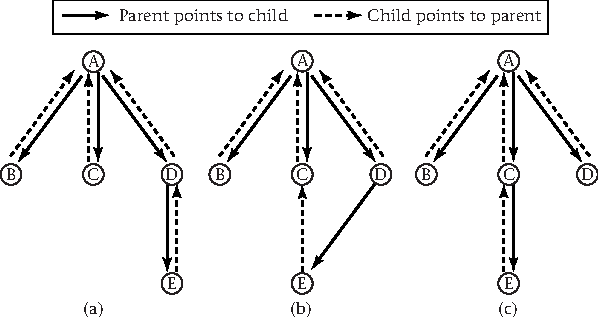
\includegraphics{hail_f0501}}
%\centerline{\epsfbox{scan-5-1.eps}}
\caption{Rooted trees with pointers to children and parents: (a)
  example satisfying the invariant; (b) invariant violated because
  E's parent is now C, but E is still a child of D and not of C;
  (c) invariant restored because the only child pointer leading to E
  again agrees with E's parent pointer.  The complete transformation
  from Part (a) to Part (c) requires modifications to nodes C, D, and E.}
\label{scan-5-1}
\end{figure}
An
invariant is that X has Y as a child if and only if Y has X as its
parent.  An operation to move a node to a new position in the tree
would need to change three objects (the node, the old parent, and the
new parent) in order to preserve the invariant.
\item
Under exceptional circumstances an operation may \vocab{fail}, that is,
be forced to give up after doing only part of its invariant-preserving
transformation.  For example, some necessary resource may be
unavailable, the user may press a Cancel button, the input may fail a
validity check, or a hardware failure may occur.  Nonetheless, the
system should be left in a consistent state.
\end{enumerate}

An \foldvocab{atomic}{transaction} is an operation that takes a system
from an observable initial state to an observable final state, without
any intermediate states being observable or perturbable by other
atomic transactions.  If a system starts with a consistent initial
state and modifies that state using only invariant-preserving
atomic transactions, the state will remain consistent.
Atomicity\index{atomic} must be preserved in the face of both
concurrency and failures.  That is, no transaction may interact with a
concurrently running transaction nor may any transaction see an
intermediate state left behind by a failed transaction.  The former
requirement is known as \vocab{isolation}.  The latter requirement
lacks a generally agreed-upon name; I will call it \vocab{failure atomicity}.

Often, atomic transactions are simply called \vocabs{transaction}.  In
fact, according to many authors, atomicity is part of the definition
of a transaction.  Unfortunately, there are other authors for whom
transactions need not be atomic.  Because of this lack of agreement on
the nomenclature, I have introduced this chapter with the full phrase
``atomic transactions'' to make my focus clear.  Henceforth, I will
skip the modifier ``atomic'' and use only ``transactions,'' with the
understanding that they are atomic unless otherwise specified.

Many transaction systems require not only atomicity, but also
\vocabindex{durability}{durable}.  A transaction is durable if the
state of a successfully completed transaction remains intact, even if
the system crashes afterward and has to be rebooted.  Each successful
transaction ends with an explicit \vocab{commit} action, which
signifies that the consistent final state has been established and
should be made visible to other transactions.  With durable
transactions, if the system crashes after the commit action, the final
transformed state will be intact after system restart.  If the crash
occurs before the commit action, the system will be back in the
initial, unchanged state after restart.

Note that failure atomicity is slightly simpler for nondurable
transactions.  Atomicity across system crashes and restarts is easy to
arrange: by clearing all memory on restart, you can guarantee that no
partially updated state is visible after the restart---no updates at
all, partial or otherwise, will remain.  This clearing of memory will
happen automatically if the computer's main semiconductor DRAM memory
is used, because that memory is \vocab{volatile}, that is, it does not
survive reboots.  (Strictly speaking, volatility means the memory does
not survive a loss of power; reboots with the power left on generally
clear volatile memory as well, however.)

Even nondurable transactions must ensure failure atomicity
for less dramatic failures in which the system is not rebooted.  For
example, a transaction might do some updates, then discover invalid
input and respond by bailing out.
To take another example, recovering from a
detected deadlock might entail aborting one of the deadlocked
transactions.  Both situations can be handled using an
explicit \vocab{abort} action, which indicates the transaction should
be terminated with no visible change made to the state.  Any changes
already made must be concealed, by undoing them.

In 1983, \index{Harder, Theo@H{\"a}rder, Theo}H{\"a}rder and
\index{Reuter, Andreas}Reuter coined a catchy phrase by saying that
whether a system supports transactions is ``the \index{ACID}ACID test of the
system's quality.''  The ACID acronym indicates that transactions are
\vocab{atomic}, \vocab{consistent}, \vocab{isolated}, and
\vocab{durable}.  This acronym is quite popular, but somewhat
redundant.  As you have seen, a transaction system really only provides
two properties: atomicity and durability.  Consistency is a property
of system states---a state is consistent if the invariants hold.
Transactions that are written correctly (so each preserves invariants)
will leave the state consistent if they execute atomically.  Isolation
simply is another name for atomicity in the face of concurrency:
concurrent transactions must not interact.

The properties of atomicity and durability refer to transactions,
independent of the objects on which the transactions operate.
Returning to the earlier rooted tree example of moving a node to a new
position, a transaction might modify the node, the old parent, and the
new parent, all within one atomic unit.  This stands in contrast
to monitors, each of which controls a single
object.

To obtain the requisite atomicity with monitors, the whole tree could
be a single monitor object, instead of having one monitor per node.  The tree
monitor would
have an operation to move one of its nodes.  In general, this approach
is difficult to reconcile with modularity. Moreover, lumping lots of
data into one monitor creates a performance problem.  Making the
whole system (or a large chunk of it) into one monitor would prevent
any concurrency.  Yet it ought to be possible to concurrently move two
nodes in different parts of a tree.  Atomic transactions allow
concurrency of this sort while still protecting the entire
transformation of the system's state.

This point is worth emphasizing.  Although the system's state remains
consistent \emph{as though} only one transaction were executed at a
time, transactions in fact execute concurrently, for performance
reasons.  The transaction system is responsible for maintaining
atomicity in the face of concurrency.  That is, it must ensure that
transactions don't interact with one another, even when running
concurrently.  Often the system will achieve this isolation by
ensuring that no transaction reads from any data object being
modified by another transaction.  Enforcing this restriction entails introducing
synchronization that limits, but does not completely eliminate, the
concurrency.

In Section~\ref{trasactions-examples-section}, I will sketch several examples of the ways in
which transactions are used by middleware and operating systems to
support application programs.  Thereafter, I present techniques used
to make transactions work, divided into three sections.  First, Section~\ref{atomicity-mechanisms-section}
explains basic techniques for ensuring the atomicity of transactions,
without addressing durability.  Second, Section~\ref{wal} explains how
the mechanism used to ensure failure atomicity can be extended to also
support durability.  Third,
Section~\ref{additional-transaction-mechanisms-section} explains a few additional mechanisms
to provide increased concurrency and
coordinate multiple participants cooperating on a single transaction.
Finally, Section~\ref{security-and-transactions-section} is devoted to security issues.
The chapter concludes with exercises, exploration and programming projects, and notes.

\section{Example Applications of Transactions}\label{trasactions-examples-section}

The transaction concept is much more pervasive in middleware than in
operating systems.  Therefore, of the three examples presented in the
following subsections, the first two are from middleware systems.
Sections \ref{db-transaction-section} and
\ref{transactions-message-queuing-systems-section} explain the two
most long-standing middleware applications, namely database systems
and message-queuing systems.
Moving into the operating systems arena, Section~\ref{jfs-transactions-section} 
explains the role that transactions play in
journaled file systems, which are the current dominant form of file
system.

\subsection{Database Systems}\label{db-transaction-section}

The transaction concept is most strongly rooted in \vocabs{database
system}; for decades, every serious database system has provided
transactions as a service to application programmers.  Database
systems are an extremely important form of middleware, used in almost
every enterprise information system.  Like all middleware,
database systems are built on top of operating system services, rather
than raw hardware, while providing  general-purpose services
to application software.  Some of those services are synchronization
services: just as an operating system provides mutexes, a database
system provides transactions.

On the other hand, transaction services are not the central, defining
mission of a database system.  Instead, database systems are primarily
concerned with providing persistent data storage and convenient means
for accessing the stored data.  Nonetheless, my goal in this chapter is to show how transactions fit
into relational database systems.  I will cover just enough of the SQL
language used by such systems to enable you to try out the example on
a real system.  In particular, I show the example using the Oracle
database system.

Relational database systems manipulate tables of data.  In Chapter~\ref{synchronization-chapter}'s
discussion of deadlock detection, I showed a
simple example from the Oracle database system involving two
accounts with account numbers 1 and 2.  The scenario
(as shown in Figure~\ref{oracle-deadlock} on
page~\pageref{oracle-deadlock}) involved transferring money from each
account to the other, by updating the balance of each account.  Thus,
that example involved a table called \verb|accounts| with two columns,
\verb|account_number| and \verb|balance|.  That table can be created
with the SQL command shown here:
\begin{verbatim}
create table accounts (
  account_number int primary key,
  balance int);
\end{verbatim}
Similarly, you can initialize account~1 to \$750 and account~2 to
\$2250 by using the following commands:
\begin{verbatim}
insert into accounts values (1, 750);
insert into accounts values (2, 2250);
\end{verbatim}
At this point, you can look at the table with the \verb|select| command:
\begin{verbatim}
select * from accounts;
\end{verbatim}
and get the following reply:
\begin{verbatim}
ACCOUNT_NUMBER    BALANCE                                                       
-------------- ----------                                                       
             1        750                                                       
             2       2250                                                       
\end{verbatim}
(If you are using a relational database other than Oracle, the format
of the table may be slightly different.  Of course, other aspects of
the example may differ as well, particularly the deadlock detection
response.)

At this point, to replicate the deadlock detection example from
Figure~\ref{oracle-deadlock}, you will need to open up two different
sessions connected to the database, each in its own window.  In the
first session, you can debit \$100 from account~1, and in the second
session you can debit \$250 from account~2.  (See
page~\pageref{oracle-deadlock} for the specific SQL commands.)  Now
in session one, try to credit the \$100 into account~2; this is blocked,
because the other session has locked account~2.  Similarly, session two
is blocked trying to credit its \$250 into account~1, creating a
deadlock, as illustrated in Figure~\ref{scan-5-2}.
\begin{figure}
\centerline{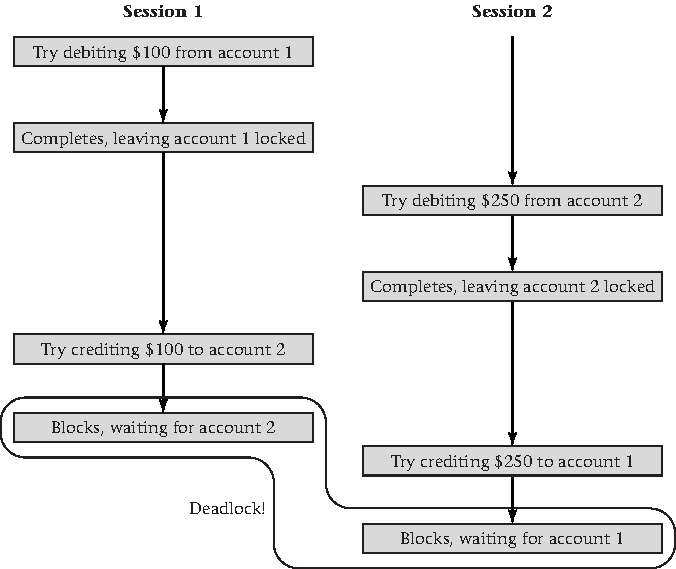
\includegraphics{hail_f0502}}
%\centerline{\epsfysize=5in\epsfbox{scan-5-2.eps}}
\caption{Two transfer transactions deadlock when each waits for
  exclusive access to the account for which the other already has
  obtained exclusive access.  In this diagram, the vertical dimension
  represents the passage of time.}
\label{scan-5-2}
\end{figure}
As you saw, Oracle detects the deadlock and chooses to cause
session one's update request to fail.

Having made it through all this prerequisite setup, you are in a
position to see the role that transactions play in situations such as
this.  Each of the two sessions is processing its own transaction.
Recall that session one has already debited \$100 from account~1 but
finds itself unable to credit the \$100 into account~2.  The
transaction cannot make forward progress, but on the other hand, you
don't want it to just stop dead in its tracks either.  Stopping would block the
progress of session two's transaction.  Session one also cannot just bail
out without any cleanup: it has already debited \$100 from account~1.
Debiting the source account without crediting the destination account
would violate atomicity and make customers angry besides.

Therefore, session one needs to abort its transaction, using the
\verb|rollback| command.  Aborting will back out of the transaction's earlier debiting
of \$100 from account~1 and release its lock on that account.  As a
result, session two's attempt to credit \$250 into account~1 can
finally stop hanging and complete.  Continuing my earlier tradition
of showing session one at the left margin and session two indented
four spaces, the interaction would look like:
\begin{verbatim}
SQL> rollback;

Rollback complete.

    1 row updated.
\end{verbatim}

Of course, whoever was trying to transfer \$100 from account~1 to
account~2 still wants to do so.  Therefore, after aborting that
transaction, you should retry it:
\begin{verbatim}
SQL> update accounts set balance = balance - 100
                     where account_number = 1;
\end{verbatim}
This command will hang, because session two's transaction now has both
accounts locked.  However, that transaction has nothing more it needs
to do, so it can commit, allowing session one to continue with its retry:
\begin{verbatim}
    SQL> commit;

    Commit complete.

1 row updated.

SQL> update accounts set balance = balance + 100 
                     where account_number = 2;

1 row updated.

SQL> commit;

Commit complete.

SQL> select * from accounts;

ACCOUNT_NUMBER    BALANCE                                                       
-------------- ----------                                                       
             1        900                                                       
             2       2100                                                       
\end{verbatim}
Notice that at the end, the two accounts have been updated correctly.
For example, account~1 does not look as though \$100 was debited from
it twice---the debiting done in the aborted transaction was wiped
away.  Figure~\ref{scan-5-3} illustrates how the transactions recover
from the deadlock.
\begin{figure}
\centerline{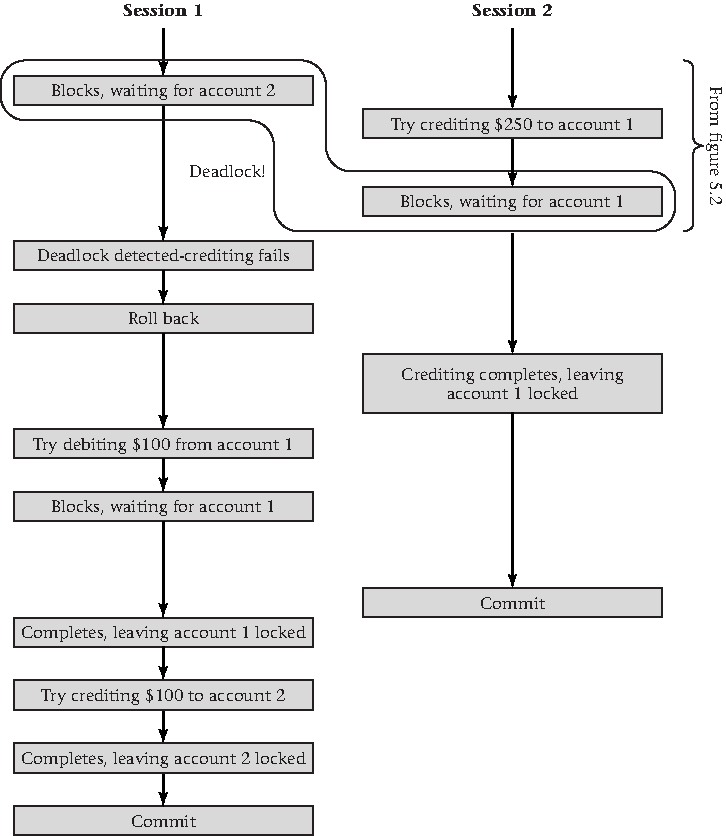
\includegraphics{hail_f0503}}
%\centerline{\epsfysize=7in\epsfbox{scan-5-3.eps}}
\caption{Transactions recover from their deadlock when one rolls back,
  releasing the lock it holds.  As in the prior figure, the vertical
  dimension represents the passage of time.}
\label{scan-5-3}
\end{figure}


In a large system with many accounts, there may be many concurrent
transfer transactions on different pairs of accounts.  Only
rarely will a deadlock situation such as the preceding example arise.
However, it is nice to know that database systems have a clean way of
dealing with them.  Any transaction can be aborted, due to deadlock
detection or any other reason, and retried later.  Moreover, concurrent
transactions will never create incorrect results due to races; that was why
the database system locked the accounts, causing the temporary hanging
(and in one case, the deadlock) that you observed.

\subsection{Message-Queuing Systems}\label{transactions-message-queuing-systems-section}

\vocabindex{Message-queuing systems}{message-queuing system} form
another important class of middleware, and like database systems, they
support the transaction concept.  
Developers of large-scale enterprise information systems normally use both forms of
middleware, although message-queuing systems are more avoidable than
database systems.
As with database systems, the
primary mission of message queuing is not the support of
transactions.  Instead, message-queuing systems specialize in the
provision of communication services. As such, I will discuss them further
in Chapter~\ref{distmid-chapter}, as part of a discussion
of the broader family of middleware to which they belong:
\vocabs{messaging system} or
\foldvocab{message-oriented}{middleware} (\vocab{MOM}).

A straightforward application of messaging consists of a server
accessed through a request queue and a response queue.  
As shown in Figure~\ref{scan-5-4}, the server
\begin{figure}
\centerline{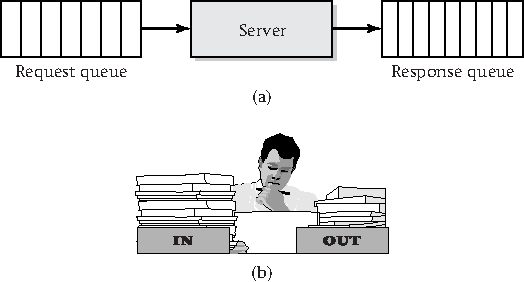
\includegraphics{hail_f0504}}
%\centerline{\epsfbox{scan-5-4.eps}}
\caption{An analogy: (a) a server dequeues a message from its request
  queue, processes the request, and enqueues a message into the response queue; (b) an
  office worker takes paper from the In basket, processes the
  paperwork, and puts it into the Out basket.}
\label{scan-5-4}
\end{figure}
dequeues a request message from the request queue, carries out the
required processing, and enqueues a response message into the response
queue.  (Think about an office worker whose desk has two baskets,
labeled ``in'' and ``out,'' and who takes paper from one, processes it, and
puts it in the other.)

These three steps (dequeue, process, enqueue) are grouped together as
an atomic transaction.  If any of the three steps fail, the request
message is left in the input queue, ready to be retried.  No request
will be lost, nor will there ever be visible signs of repeated
processing, such as duplicated response messages.  (Of course, some
causes of failure will affect retries as well.  For that reason,
realistic systems generally keep count of retries and after a while
divert the request message, for example, into a human troubleshooter's
request queue.)

Message-queuing systems also provide durability, so that even if the system crashes and restarts,
each request will generate exactly one response.
In most systems, applications can opt out of durability in order to reduce persistent storage traffic and thereby
obtain higher performance.

To provide greater concurrency, a system may have several servers
dequeuing from the same request queue, as shown in
Figure~\ref{scan-5-5}.
\begin{figure}
\centerline{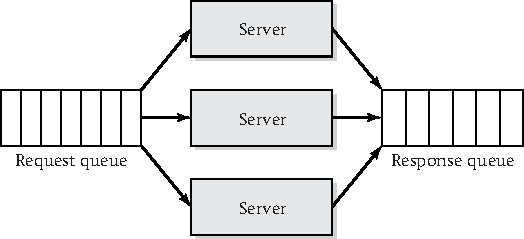
\includegraphics{hail_f0505}}
%\centerline{\epsfbox{scan-5-5.eps}}
\caption{Several message-driven servers in parallel can dequeue from a
  common request queue and enqueue into a common response queue.  To
  allow concurrent operation, messages need not be provided in strict
  first-in, first-out order.}
\label{scan-5-5}
\end{figure}
This configuration has an interesting
interaction with atomicity.  If the dequeue action is interpreted
strictly as taking the message at the head of the queue, then you have
to wait for the first transaction to commit or abort before you can
know which message the second transaction should dequeue.  (If the
first transaction aborts, the message it tried to dequeue is still at
the head of the queue and should be taken by the second
transaction.)  This would prevent any concurrency.  Therefore,
message-queuing systems generally relax queue ordering a little,
allowing the second message to be dequeued even before the fate of the
first message is known.  In effect, the first message is provisionally
removed from the queue and so is out of the way of the second
message.  If the transaction handling the first
message aborts, the first message is returned to the head of the queue, even though the
second message was already dequeued.

More advanced \vocab{workflow} systems may include
several processing steps, with each processing step connected to the
next by an intermediate message queue. In these systems, each
processing stage is treated as a separate transaction.  If the
transaction commits, that stage's input is gone from its inbound
queue, and its output is in the outbound queue.  Seen as a whole, the
workflow may not exhibit atomicity.  For example, failure in a later
processing stage will not roll back an earlier stage.

Consider a sale of merchandise as an example workflow, as shown in
Figure~\ref{scan-5-6}.
\begin{figure}
\centerline{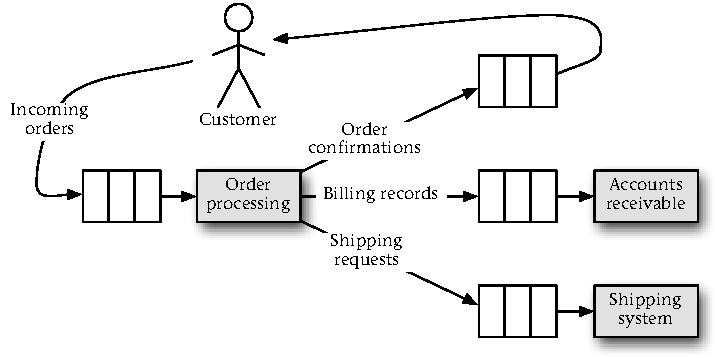
\includegraphics{hail_f0506}}
%\centerline{\epsfbox{scan-5-6.eps}}
\caption{In this simplified workflow for selling merchandise,
  processing a single order produces three different responses.  The
  response queues from the order-processing step are request queues
  for subsequent steps.}
\label{scan-5-6}
\end{figure}
One transaction might take an incoming order, check it for validity,
and generate three output messages, each into its own outbound queue:
an order confirmation (back to the customer), a billing record (to the
accounts receivable system), and a shipping request (to the shipping
system).  Another transaction, operating in the shipping
system, might dequeue the shipping request and fulfill it.  If
failure is detected in the shipping transaction, the system can no longer
abort the overall workflow; the order confirmation and
billing have already been sent.  Instead, the shipping transaction has
no alternative but to drive the overall workflow forward, even if in
a somewhat different direction than hoped for.  For example, the
shipping transaction could queue messages apologizing to the customer
and crediting the purchase price back to the customer's account.
Figure~\ref{scan-5-7} shows the workflow with these extra steps.
\begin{figure}
\centerline{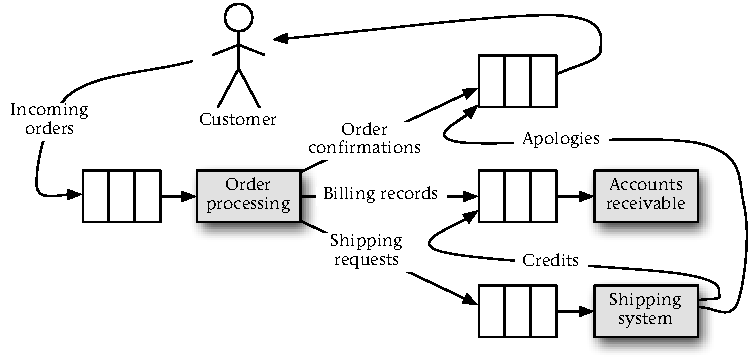
\includegraphics{hail_f0507}}
%\centerline{\epsfbox{scan-5-7.eps}}
\caption{In this workflow, a failure in shipping must produce
  compensating responses, as it cannot abort the
  overall workflow.  The compensating responses credit the
  customer's account for the previously debited amount and send an
  apology to the customer indicating that the previously confirmed
  order will not be filled after all.}
\label{scan-5-7}
\end{figure}

Even in a system in which one transaction may bill the
customer only to have a later \vocab{compensating transaction} refund
the billed amount, using atomic transactions simplifies application
programming.  Imagine how complex it would be to reason about a
large workflow if each individual processing stage could fail midway through or
could interact with other concurrently executing stages.  By treating
each workflow stage as an atomic transaction, a messaging system
considerably reduces the application designer's cognitive burden.  A
diagram, such as Figure~\ref{scan-5-7}, can provide an accurate abstraction of the system's observable
behaviors by showing the system as processing stages linked by message
queues.

Finally, consider how the sales workflow keeps track of available
merchandise, customer account balances, and other information.  You
should be able to see that individual processing stages of a workflow
will frequently have to use a database system.  As such, transactions
will involve both message queues and databases.  Atomicity needs to
cover both; if a transaction aborts, you want the database left
unchanged \emph{and} the request message left queued.  In
Section~\ref{two-phase-commit-section}, I will explain how this
comprehensive atomicity can be achieved by coordinating the systems
participating in a transaction.

\subsection{Journaled File Systems}\label{jfs-transactions-section}

The transaction concept has been employed in middleware both longer
and more extensively than in operating systems.  However, one
application in operating systems has become quite important.  Most
contemporary operating systems provide file systems that employ atomic
transactions to at least maintain the structural consistency of the
file system itself, if not the consistency of the data stored in
files.  These file systems are known as
\foldvocabs{journaled}{file system} (or
\foldvocabs{journaling}{file system}) in reference to their use of an
underlying mechanism known as a \vocab{journal}. I will discuss
journals in Sections \ref{failure-atomicity-subsection} and \ref{wal} under their alternative name,
\vocabs{log}.  Examples of journaled file systems include NTFS, used
by Microsoft Windows; HFS Plus, used by Mac OS~X; and ext3fs, reiserfs, JFS, and XFS, used by Linux.  (The latter two
originated in proprietary UNIX systems: JFS was developed by IBM for
AIX, and XFS was developed by SGI for IRIX.)  File systems that are
not journaled need to use other techniques, which I describe in
Section~\ref{metadata-integrity-section}, to maintain the consistency of
of their data structures.

File systems provide a more primitive form of data storage and access
than database systems.  As you will see in Chapter~\ref{persistence-chapter}, contemporary
operating systems generally treat a file as an arbitrarily large,
potentially extensible sequence of bytes, accessed by way of a
textual name.  The names are organized hierarchically into nested
directories or folders.  Typical operations on files include create,
read, write, rename, and delete.

Underlying this simple abstraction are some largely invisible
data structures, known as \vocab{metadata}, that help locate and
organize the data.  For example, because each file can grow in size,
the file system must be free to store different parts of a file in
different locations.  As such, the file system must store
metadata for each file indicating where each portion of the
file is located.  Moreover, the file system must store information concerning
what parts of the storage are in use, so that it can allocate unused
space for a file that is growing.

The existence of this metadata means that even simple file operations
can involve several updates to the information in persistent storage.
Extending a file, for example, must update both the information about
free space and the information about space allocated to that file.
These structures need to be kept consistent; it would be
disastrous if a portion of the storage were both used for storing a file
and made available for allocation to a second file.  Thus, the updates
should be done as part of an atomic transaction.

Some atomic transactions may even be visible to the user.  Consider
the renaming of a file.  A new directory entry needs to be created and an old
entry removed.  The user wants these two changes done atomically,
without the possibility of the file having both names, or neither.

Some journaled file systems treat each operation requested by an
application program as an atomic and durable transaction.  On such a system, if a
program asks the system to rename a file, and the rename operation
returns with an indication of success, the application program can be
sure that renaming has taken place.  If the system crashes immediately
afterward and is rebooted, the file will have its new name.  Said
another way, the rename operation includes commitment of the
transaction.  The application program can tell that the transaction
committed and hence is guaranteed to be durable.

Other journaled file systems achieve higher performance by delaying
transaction commit.  At the time the rename operation returns, the
transaction may not have committed yet.  Every minute or so, the file
system will commit all transactions completed during that interval.
As such, when the system comes back from a crash, the file system will
be in some consistent state, but maybe not a completely up-to-date one.
A minute's worth of operations that appeared to complete
successfully may have vanished.  In exchange for this risk, the system
has gained the ability to do fewer writes to persistent storage, which improves
performance.  Notice that even in this version, transactions are
providing some value.  The state found after reboot will be the result
of some sequence of operations (even if possibly a truncated
sequence), rather than being a hodgepodge of partial results from
incomplete and unordered operations.

Often, journaled file systems protect only metadata; the application
data stored in files may be left in an inconsistent state after a
crash.
In particular, some writes into the files may not have taken effect, and the writes that are lost in this way are not necessarily the ones performed most recently.
Even many journaled file system that do better than
this offer only a guarantee that all write operations
that completed before a crash will be reflected in the state after the
crash.  With this limited guarantee, if a program wants to do multiple writes in an atomic fashion
(so that all writes take place or none do), the file system will not
provide any assistance.  However, a file system can also be designed to
fully support transactions, including allowing the programmer to
group multiple updates into a transaction.  One example of such a fully
transactional file system is Transactional NTFS (TxF), which was added
to Microsoft Windows in the Vista version.

\section{Mechanisms to Ensure Atomicity}\label{atomicity-mechanisms-section}

Having seen how valuable atomic transactions are for middleware and
operating systems, you should be ready to consider how this value is
actually provided.  In particular, how is the atomicity of each
transaction ensured?  Atomicity has two aspects: the isolation of
concurrent transactions from one another and the assurance that
failed transactions have no visible effect.  In
Section~\ref{two-phase-section}, you will see how isolation is
formalized as serializability and how a particular locking discipline,
two-phase locking, is used to ensure serializability.  In
Section~\ref{failure-atomicity-subsection}, you will see how failure
atomicity is assured through the use of an undo log.

\subsection{Serializability: Two-Phase Locking}\label{two-phase-section}

Transactions may execute concurrently with one another, so long as
they don't interact in any way that makes the concurrency apparent.
That is, the execution must be equivalent to a \vocab{serial}
execution, in which one transaction runs at a time, committing or
aborting before the next transaction starts.  Any execution
equivalent to a serial execution is called a \vocab{serializable} execution.  In
this section, I will more carefully define what is means for two
executions to be equivalent and hence what it means for an execution
to be serializable.  In addition, I will show some simple rules for using
readers/writers locks that guarantee serializability.  These rules,
used in many transaction systems, are known as
\foldvocab{two-phase}{locking}.

Equivalence, and hence serializability, can be defined in several
somewhat different ways.  The definitions I give are the simplest I
could find and suffice to justify two-phase locking, which is the
mechanism normally used to achieve serializability in practical
systems.  However, you should be aware that more general definitions
are needed in order to accommodate more advanced concurrency control
mechanisms.  The notes at the end of the chapter provide pointers to
some of these more sophisticated alternatives.

Each transaction executes a sequence of actions.  I will focus on
those actions that read or write some stored entity (which might be a
row in a database table, for example) and those actions that lock or
unlock a readers/writers lock.  Assume that each stored entity
has its own lock associated with it.  I will use the following
notation:
\begin{itemize}
\item
$r_j(x)$ means a read of entity $x$ by transaction $T_j$; when I want
  to show the value that was read, I use $r_j(x, v)$, with $v$ as the value.
\item
$w_j(x)$ means a write of entity $x$ by transaction $T_j$; when I want
  to show the value being written, I use $w_j(x, v)$, with $v$ as the value.
\item
$s_j(x)$ means an acquisition of a shared (that is, reader) lock on entity $x$ by transaction $T_j$.
\item
$e_j(x)$ means an acquisition of an exclusive (that is, writer) lock on
  entity $x$ by transaction $T_j$.
\item
$\overline{s}_j(x)$ means an unlocking of a shared lock on entity $x$ by transaction $T_j$.
\item
$\overline{e}_j(x)$ means an unlocking of an exclusive lock on entity
  $x$ by transaction $T_j$.
\item
$u_j(x)$ means an upgrade by transaction $T_j$ of its hold on entity
  $x$'s lock from shared status to exclusive status.
\end{itemize}
Each read returns the most recently written value.  Later, in
Section~\ref{reduced-isolation}, I will revisit this assumption,
considering the possibility that writes might store each successive
value for an entity in a new location so that reads can choose
among the old values.

The sequence of actions executed by a transaction is called its
\vocab{history}.
Because the transactions execute concurrently, if you were to write
all their actions in the order they happen, the transactions'
histories would be interleaved.
This time-ordered interleaving of all the
transactions' histories is called the system's history.  All locking actions
are shown at the time when the lock is granted, not at the possibly
earlier time when the lock is requested.  Assume that the histories
include all the relevant actions.  In particular, if a transaction
aborts and does some extra writes at that time to undo the effect of
earlier writes (as you will see in Section~\ref{failure-atomicity-subsection}),
those undo writes must be explicitly listed in the history.  Note
also that I am implicitly assuming the transactions have no effects
other than on storage; in particular, they don't do any I/O.

Let's look at some examples.  Suppose that $x$ and $y$ are two
variables that are initially both equal to 5.
Suppose that transaction $T_1$ adds 3 to each of the two
variables, and transaction $T_2$ doubles each of the two variables.
Each of these transactions preserves the invariant that
$x=y$.

One serial history would be as follows:
\begin{eqnarray*}
&&e_1(x), r_1(x, 5), w_1(x, 8), \overline{e}_1(x),
  e_1(y), r_1(y, 5), w_1(y, 8), \overline{e}_1(y),\\
&&e_2(x), r_2(x, 8), w_2(x, 16), \overline{e}_2(x),
  e_2(y), r_2(y, 8), w_2(y, 16), \overline{e}_2(y)
\end{eqnarray*}
Before you go any further, make sure you understand this notation; as directed in
Exercise~\ref{t2-first-ex}, write out another serial history in which transaction
$T_2$ happens before transaction $T_1$.  (The sequence of steps within each
transaction should remain the same.)

In the serial history I showed, $x$ and $y$ both end up with the value
16.  When you wrote out the other serial history for these two transactions,
you should have obtained a different final value for these variables.  Although
the invariant $x=y$ again holds, the common numerical value of $x$ and
$y$ is not 16 if transaction $T_2$ goes first.  This makes an important
point: transaction system designers do not insist on \vocab{deterministic} execution,
in which the scheduling cannot affect the result.  Serializability is a
weaker condition.

Continuing with the scenario in which $T_1$ adds 3 to each variable
and $T_2$ doubles each variable, one serializable---but not serial---history follows:
\begin{eqnarray*}
&&e_1(x), r_1(x, 5), w_1(x, 8), \overline{e}_1(x),
  e_2(x), r_2(x, 8), w_2(x, 16), \overline{e}_2(x),\\
&&e_1(y), r_1(y, 5), w_1(y, 8), \overline{e}_1(y),
  e_2(y), r_2(y, 8), w_2(y, 16), \overline{e}_2(y)
\end{eqnarray*}
To convince others that this history is serializable, you could
persuade them that it is equivalent to the serial history shown
previously.  Although transaction $T_2$ starts before transaction $T_1$ is
finished, each variable still is updated the same way as in the
serial history.

Because the example transactions unlock $x$ before locking $y$, they
can also be interleaved in a nonserializable fashion:
\begin{eqnarray*}
&&e_1(x), r_1(x, 5), w_1(x, 8), \overline{e}_1(x),
  e_2(x), r_2(x, 8), w_2(x, 16), \overline{e}_2(x),\\
&&e_2(y), r_2(y, 5), w_2(y, 10), \overline{e}_2(y),
  e_1(y), r_1(y, 10), w_1(y, 13), \overline{e}_1(y)
\end{eqnarray*}
Here, the invariant $x=y$ is broken: at the end, $x$ is equal to 16,
but $y$ is equal to 13.  Thus, this history is not equivalent to
either of the two serial histories.

My primary goal in this section is to show how locks can be used in a
disciplined fashion that rules out nonserializable histories.  (In
particular, you will learn that in the previous example, $x$ should not be
unlocked until after $y$ is locked.)  First, though, I need to
formalize what it means for two histories to be equivalent, so that
the definition of serializability is rigorous.

I will make two assumptions about locks:
\begin{enumerate}
\item
Each transaction correctly pairs up lock and unlock operations.  That
is, no transaction ever locks a lock it already holds (except
upgrading from shared to exclusive status), unlocks a lock it doesn't
hold, or leaves a lock locked at the end.
\item
The locks function correctly.  No transaction will ever be granted a
lock in shared mode while it is held by another transaction in
exclusive mode, and no transaction will ever be granted a lock in
exclusive mode while it is held by another transaction in either
mode.
\end{enumerate}
Neither of these assumptions should be controversial.

Two system histories are equivalent if the first history can be turned
into the second by performing a succession of equivalence-preserving
swap steps.  An equivalence-preserving swap reverses the order of
two adjacent actions, subject to the following constraints:
\begin{itemize}
\item
The two actions must be from different transactions.  (Any
transaction's actions should be kept in their given order.)
\item
The two actions must not be any of the following seven \vocabindex{conflicting}{conflict} pairs:
\begin{enumerate}
\item
$\overline{e}_j(x), s_k(x)$
\item
$\overline{e}_j(x), e_k(x)$
\item
$\overline{s}_j(x), e_k(x)$
\item
$\overline{s}_j(x), u_k(x)$
\item
$w_j(x),r_k(x)$
\item
$r_j(x),w_k(x)$
\item
$w_j(x),w_k(x)$
\end{enumerate}
Forbidding swaps of the first four pairs ensures locks continue properly
functioning: $T_k$ may not lock $x$'s lock until after $T_j$ has
unlocked it.  The next two conflicts ensure the read actions return the correct
values: swapping a read and a write would change which value the read action returns.  The final conflict ensures that
$x$ is left storing the correct value.
\end{itemize}

Figure~\ref{scan-5-8} illustrates some of the constraints on
equivalence-preserving swaps.
\begin{figure}
\centerline{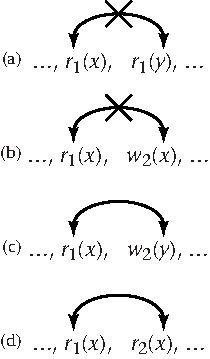
\includegraphics{hail_f0508}}
%\centerline{\epsfbox{scan-5-8.eps}}
\caption{Illegal and legal swaps: (a) illegal to swap steps from one
  transaction; (b) illegal to swap two conflicting operations on the
  same entity; (c) legal to swap operations on different entities by
  different transactions; (d) legal to swap nonconflicting operations by
  different transactions.}
\label{scan-5-8}
\end{figure}
Note that in all the conflicts, the two actions operate on the same
stored entity (shown as $x$); any two operations on different entities
by different transactions
can be reversed without harm.  In Exercise~\ref{serializing-ex},
show that this suffices
to prove that the earlier example of a serializable history is indeed
equivalent to the example serial history.

Even if two actions by different transactions involve
the same entity, they may be reversed without harm if they are both reads.
Exercise~\ref{reads-commute-ex} includes a serializable
history where reads of an entity need to be reversed in order to
arrive at an equivalent serial history.

I am now ready to state the two-phase locking rules, which suffice
to ensure serializability.  For now, concentrate on understanding what
the rules say; afterward I will show that they suffice.  A
transaction obeys two-phase locking if:
\begin{itemize}
\item
For any entity that it operates on, the transaction locks the
corresponding lock exactly once, sometime before it reads or writes
the entity the first time, and unlocks it exactly once, sometime after
it reads or writes the entity the last time.
\item
For any entity the transaction writes into, either the
transaction initially obtains the corresponding lock in exclusive mode,
or it upgrades the lock to exclusive mode sometime before writing.
\item
The transaction performs all its lock and upgrade actions before performing any of
its unlock actions.
\end{itemize}

Notice that the two-phase locking rules leave a modest amount of
flexibility regarding the use of locks.  Consider the
example transactions that read and write $x$ and then read and write
$y$.  Any of the following transaction histories for $T_1$ would obey
two-phase locking:
\begin{itemize}
\item \label{two-phase-examples}$e_1(x), r_1(x), w_1(x), e_1(y), \overline{e}_1(x), r_1(y), w_1(y),
\overline{e}_1(y)$
\item $e_1(x), e_1(y), r_1(x), w_1(x), r_1(y), w_1(y),
\overline{e}_1(y), \overline{e}_1(x)$
\item $s_1(x), r_1(x), u_1(x), w_1(x), s_1(y), r_1(y), u_1(y),
w_1(y), \overline{e}_1(x), \overline{e}_1(y)$
\end{itemize}
In Exercise~\ref{two-phase-orders-ex}, you can come up with several additional two-phase
possibilities for this transaction.

If the programmer who writes a transaction explicitly includes the
lock and unlock actions, any of these possibilities would be valid.
More commonly, however, the programmer includes only the
reads and writes, without any explicit lock or unlock actions.  An
underlying transaction processing system automatically inserts the
lock and unlock actions to make the programming simpler and
less error-prone.  In this case, the system is likely to use
three very simple rules\label{simple-two-phase}:
\begin{enumerate}
\item
Immediately before any read action, acquire the corresponding lock in
shared mode if the transaction doesn't already hold it.
\item
Immediately before any write action, acquire the corresponding lock in
exclusive mode if the transaction doesn't already hold it.  (If the
transaction holds the lock in shared mode, upgrade it.)
\item
At the very end of the transaction, unlock all the locks the
transaction has locked.
\end{enumerate}
You should be able to convince yourself that these rules are a special
case of two-phase locking.  By holding all the locks until the end of
the transaction, the system need not predict the transaction's future
read or write actions.

I still need to prove that two-phase locking suffices to ensure
serializability.  Recall that a history is serializable if it is
equivalent to a serial history.  Thus, I need to show that so long as
two-phase locking is followed, you can find a sequence of
equivalence-preserving swaps that will transform the system history
into a serial one.  Please understand that this transformation of the
history into a serial one is just a proof technique I am using to
help understand the system, not something that actually occurs during
the system's operation.  Transaction systems are not in the business
of forcing transactions to execute serially; concurrency is good for
performance.  If anything, the running transaction system is doing the
reverse transformation: the programmer may have thought in terms of
serial transactions, but the system's execution interleaves them.  I
am showing that this interleaving is equivalence-preserving by
showing that you can back out of it.

To simplify the proof, I will use the following
vocabulary:
\begin{itemize}
\item
The portion of the system history starting with $T_j$'s first action
and continuing up to, but not including, $T_j$'s first unlock action
is \label{phase-one-definition}\vocab{phase one} of $T_j$.
\item
The portion of the system history starting with $T_j$'s first unlock
action and continuing up through $T_j$'s last action is \vocab{phase
two} of $T_j$.
\item
Any action performed by $T_k$ during $T_j$'s phase one (with $j \neq
k$) is a \foldvocab{phase one}{impurity} of $T_j$.  Similarly, any
action performed by $T_k$ during $T_j$'s phase two (with $j \neq k$)
is a \foldvocab{phase two}{impurity} of $T_j$.
\item
If a transaction has no impurities of either kind, it is
\vocab{pure}.  If all transactions are pure, then the system history
is serial.
\end{itemize}

My game plan for the proof is this.  First, I will show how to use
equivalence-preserving swaps to purify any one transaction, say, $T_j$.
Second, I will show that if $T_k$ is already pure, purifying $T_j$
does not introduce any impurities into $T_k$.  Thus, you can
purify the transactions one at a time, without having to worry about
wrecking the transactions purified earlier.

If $T_j$ is impure, you can purify it by first removing any phase one
impurities and then any phase two impurities.  To remove the phase
one impurities, you can remove the leftmost one, and then repeat with
the new leftmost one, until all are gone.  The leftmost phase one
impurity of $T_j$ must be preceded by an action of $T_j$.  I will
show that those two actions can be reversed by an
equivalence-preserving swap.  That moves the leftmost impurity
further to the left.  If this swapping is done repeatedly, the
impurity will percolate its way further and further to the left until
it passes the first operation of $T_j$, at which point it will cease
to be an impurity of $T_j$.  Phase two impurities can be removed
similarly, starting with the rightmost one, by percolating them to the
right until they pass the last operation of $T_j$.

I need to show that the leftmost phase one impurity of $T_j$ can be
swapped with its left-hand neighbor, and that the rightmost phase two
impurity can be swapped with it right-hand neighbor.  Recall that to
legally swap two actions, they must be from different transactions,
and they must not be one of the seven forbidden conflicting pairs.  In
order to be the leftmost impurity of $T_j$, an action must be
performed by some other transaction, $T_k$, and have an action from
$T_j$ as its left-hand neighbor.  (A similar argument applies for the rightmost
impurity and its right-hand neighbor.)  Thus, the actions are
definitely from different transactions, and the only remaining concern is
the seven conflicts.

For the leftmost phase one impurity and its left-hand neighbor, you
cannot have any of these conflicts:
\begin{enumerate}
\item $\overline{e}_j(x), s_k(x)$
\item $\overline{e}_j(x), e_k(x)$
\item $\overline{s}_j(x), e_k(x)$
\item $\overline{s}_j(x), u_k(x)$
\end{enumerate}
because transaction $T_j$ does not do any unlock actions in phase one.
(Recall the definition of phase one.)  Nor can you have any of the
other three conflicts:
\begin{enumerate}[resume]
\item $w_j(x), r_k(x)$
\item $r_j(x), w_k(x)$
\item $w_j(x), w_k(x)$
\end{enumerate}
because the two-phase locking rules ensure that each read or write action is performed only with the
appropriate lock held.  There is no way transactions $T_j$ and $T_k$
can both hold the lock on $x$, with at least one of them being in
exclusive mode.  Similar arguments rule out any conflict between the
rightmost phase two impurity and its right-hand neighbor; in
Exercise~\ref{phase-two-purification-ex}, you can fill in the details.

You have now seen that equivalence-preserving swap steps suffice to
purify $T_j$ by percolating each of its phase one impurities out to
the left and each of its phase two impurities out to the right.  The
goal is to serialize an arbitrary system history that complies with
the two-phase locking rules.  I would like to pick one of its
transactions that is impure and purify it, then repeat with another
and keep going until all the transactions are pure, that is, until the system
history has become serial.  For this plan to work, I need to be sure
that purifying one transaction doesn't wreck the purity of any already
pure transaction.

Purifying $T_j$ doesn't touch any actions that don't lie between
$T_j$'s first action and its last action.  Thus, the only way
purifying $T_j$ could endanger the existing purity of $T_k$ is if
$T_k$ lies at least partly within $T_j$'s span.  However, because $T_k$
is pure, either all of it lies within $T_j$'s span or none of it does,
so you need only consider the case that all of $T_k$ lies within
$T_j$'s span.  In fact, you should be able to convince yourself of
something stronger: if any action of a pure transaction $T_k$ lies within $T_j$'s span,
then all of $T_k$ lies within a single one of $T_j$'s phases (either
all within phase one, or all within phase two).

If $T_k$'s actions occupy consecutive positions within phase one,
purifying $T_j$ will percolate all of $T_k$'s actions to the left and
leave them in consecutive positions preceding the start of $T_j$.
Similarly, if $T_k$ is within phase two, all its actions will
move to the right and wind up as a consecutive block to the right of
$T_j$.  Thus, $T_k$'s purity is preserved.

You can conclude, then, that any system history obeying the two-phase
locking rules is serializable.  Recall that serializable histories are
equivalent to serial histories.  In a serial history composed from
invariant-preserving transactions, each transaction moves the system from one
consistent state to another.   Thus, so long as two-phase locking is
used, the system will behave as though it is moving from consistent
state to consistent state.  In particular, this
situation can be obtained simply by locking each entity before
operating on it the first time and holding all locks until the end of
the transaction.

Even though serializable histories are equivalent to serial histories,
they differ in one important regard.  Unlike a serial history, a
serializable history may include concurrency between transactions.
This allows the system to achieve higher performance but entails a
risk of deadlock that is not present in serial execution.  If deadlock
occurs, one of the deadlocked transactions needs to be aborted.  This
abortion is one way in which a transaction can fail.  Therefore, I
will next turn to the question of how atomicity is preserved in the
face of transaction failures.

\subsection{Failure Atomicity: Undo Logging}\label{failure-atomicity-subsection}
\foldindex{failure}{atomicity}
Recall that atomic transactions may temporarily put the system in an
inconsistent state so long as they restore
consistency before committing.  For example, in the middle of a transfer from one
account to another, money can temporarily ``disappear'' (not be in any
account) so long as the money has
``reappeared'' in the destination account by the time the transfer is over.  You have already seen one
way to protect against harm from these temporary inconsistencies: by
using two-phase locking, you prevent any concurrent transaction from
being affected by the inconsistent state.  Now you need to deal with
another possible source of trouble: what if a transaction aborts after
making some, but not all, of its updates to the state?  How can you
prevent later transactions from seeing an inconsistent state?

Transactions fail for many reasons.  For example, the transfer
transaction might debit money from the source account, and then before
crediting it to the destination account, discover that the destination
account doesn't exist.  Alternatively, the system might detect a deadlock when
trying to lock the destination account.  Either way, the transaction
is aborted after having debited the source account.  To keep the
transaction atomic (and thus preserve consistency), you need to undo
the debit from the source account.  That way, the failed transaction
will have left the system's state unchanged.  That is one of the two
legal outcomes of an atomic transaction: all or nothing.

Without support from a transaction processing system, failure
atomicity is extremely difficult to ensure.  Programmers write a lot
of complex and bug-prone code in attempts to provide failure atomicity
on their own.  To see how troublesome it can be, consider two ways to
achieve failure atomicity without a transaction processing system.

One approach is to try to test for all possible causes
of failure before taking any action.  For example, test that the
destination account exists, and can be locked, before debiting from
the source account.  This can lead to poor modularity.  After all, the
logical place to check the destination account is in association with
crediting that account.  In addition, the advance checking approach doesn't
cope well with concurrency.  What if a concurrent thread messed with
the destination account after it had been checked?

Another approach is to test for each possible
failure as it may occur
and provide manual cleanup actions.  For example, if a failure occurs
while crediting the destination account, revert the money back
into the source account.  The problem here is that in a complicated
transaction, many failure handlers are needed, as shown in
Figure~\ref{scan-5-9}.
\begin{figure}
\centerline{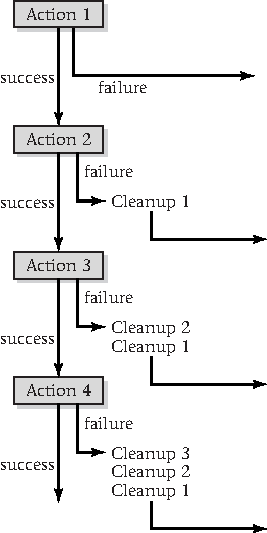
\includegraphics{hail_f0509}}
%\centerline{\epsfbox{scan-5-9.eps}}
\caption{Failure atomicity can be ensured by testing for failure
  at each step in a process and providing appropriate failure
  handlers.  The failure handler for each action needs to clean up all
  prior actions, that is, remove their effects.  This approach does
  not scale as well as the general undo log used by
  transaction processing systems.}
\label{scan-5-9}
\end{figure}
The handler for the
second action needs to undo the first action.  The handler for the
third action needs to undo actions two and one.  The handler for the
fourth action needs to undo actions three, two, and one.  In
Exercise~\ref{quadratic-undo-ex}, you can show that failure handlers must share cleanup code to prevent a quadratic increase in the
amount of code for the transaction.  Even if the failure handlers
share cleanup code, manual cleanup actions significantly complicate
the structure of the transaction.

By contrast, systems that support transactions (such as database
systems) make failure atomicity completely transparent to the
application programmer.  If a transaction aborts, the system
automatically cleans up the state so that no other transaction will
observe any effects from the aborted transaction.  In order to provide
this service, the transaction system normally uses an
\foldvocab{undo}{log}, as I will now describe.

Conceptually, each transaction has its own undo log, which records the
actions needed to back out of the changes that transaction has made to
the system's state.  Every time the transaction writes a new value
into some stored entity, it also adds an entry to the undo log,
showing how the entity can be restored to its prior state.  The
simplest way to do this is to record the old value of the
entity.

Suppose $x=5$ and transaction $T_1$ asks the
transaction processing system to write an $8$ into $x$.  In the prior section, you saw
that behind the scenes this action might do more than just write the
8 into $x$: it might first acquire an exclusive lock on $x$.  Now, you
learn that the transaction processing system will do even more behind
the scenes: it will also add an entry to $T_1$'s undo log, showing
that $x$ needs to be set back to 5 to undo this step.  That entry in
the undo log will list $x$ as the entity in question, and 5 as its
prior value.

If a transaction aborts, the transaction processing system will read
back through that transaction's undo log entries, from the most recent
to the earliest, and carry out each of the reversions listed in the
log.  Be sure you understand why the undo log entries need to be
processed in reverse chronological order.  In Exercise~\ref{reverse-chron-undo-ex}, you can
give an example where this matters.

Notice that undoing write operations involves more writing; to undo the write of
8 into $x$, you write 5 back into $x$. This has an important
consequence for two-phase locking.  If a transaction writes an entity,
it must hold the corresponding lock in exclusive mode until the
transaction has finished aborting or committing.  Shared-mode locks,
for entities that the transaction only reads, can be dropped earlier,
subject to the usual two-phase rules.  However, the exclusive-mode locks
need to be retained, because so long as the possibility of aborting
exists, the possibility of more writing exists.

I mentioned that conceptually each transaction has its own undo log.
Normal transaction processing systems actually store all the undo logs
in one combined log, with each entry added at the end.  In order to
efficiently process the entries from a single transaction in reverse
chronological order, each entry contains a pointer to the previous
entry from the same transaction.  Each transaction keeps a
pointer to its latest entry, as shown in Figure~\ref{scan-5-11}.
\begin{figure}
\centerline{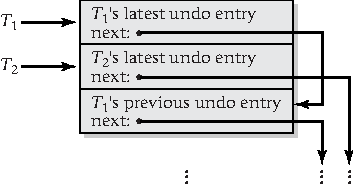
\includegraphics{hail_f0510}}
%\centerline{\epsfbox{scan-5-11.eps}}
\caption{Rather than having a separate undo log for each transaction,
  the undo logs can be combined.  In this case, the entries for any one
  transaction are chained together, as shown here, so that they can be
  efficiently processed as though in a separate log.}
\label{scan-5-11}
\end{figure}
You'll see in Section~\ref{wal} that
durability requires additional logging; these extra log entries are
also mixed into the same combined log with all the transactions' undo
entries.

\section{Transaction Durability: Write-Ahead Logging}
\label{wal}

Adding durability to transactions raises two new issues---one directly and
one indirectly:
\begin{enumerate}
\item
The direct issue is durability itself.  When a transaction commits,
all the data needs to be stored somewhere \vocab{persistent} and made
available again after system restart.  (Persistent storage might be
flash memory or a disk drive.)
\item
The indirect issue is that failure atomicity now needs more work.
When the system is restarted, it may need to clean up after
transactions that were in progress at the time the system crashed and
that had already done some writing to persistent storage.
\end{enumerate}

The simplest way to ensure durability itself is to store all entities
in persistent storage; all writing by transactions goes directly into
that persistent storage.  This is not terribly efficient; consider,
for example, the difference in speed between disk drives and RAM.
Therefore, I will explain a more practical alternative later in this section.  First,
though, to have a correct (if inefficient) solution, I need to
address failure atomicity.

When a transaction aborts, the undo log allows the system to roll back any
writes the transaction did.  If a transaction is in progress when the
system crashes, the transaction should be aborted at system
restart time, so that its partial updating of the system state is not
visible.  This abortion upon restart can be done in the usual way, by
using the undo log, if four precautions are taken:
\begin{enumerate}
\item
The undo log must be stored in persistent storage so that it will be
available when the system is
restarted, for use in what is called \vocab{recovery processing}.
\item
Whenever a transaction writes a new value for an entity into
persistent storage, it must \emph{first} write the undo record into
the persistent undo log, as shown in Figure~\ref{scan-5-13}.
\begin{figure}
\centerline{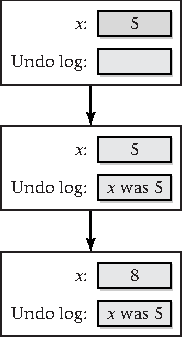
\includegraphics{hail_f0511}}
%\centerline{\epsfbox{scan-5-13.eps}}
\caption{In order to allow crash recovery, the undo log entry must be
  made persistent before the write to the underlying object.}
\label{scan-5-13}
\end{figure}
I previously did not emphasize the order
in which these two writes occur.  Now it really matters, because the
system could crash between the first write and the second.  Users cannot
risk the possibility that the entity has been written without the
undo record.
\item
The undo operation (intended to restore an entity from its new value
to its old value) must be safe to use, even if the entity already has
its old value.  In other words, the undo operation must be
\vocab{idempotent}.  Idempotency is important if the system
crashes after the undo record is written, but before the entity itself
is written.  Recovery processing can still ``undo'' the write that was
never done.  In addition, if the system crashes again in the middle of
recovery, you can start it all over again from the beginning, without
harm from repeated undo processing.  The form of
undo record that I have shown, which records the entity's old value, naturally
provides idempotency.
\item
The recovery processing must have some way to figure out what
transactions were in progress and hence need aborting.  The usual way
to do this is to keep all the undo logs in one combined log, which
also includes explicit records any time a transaction commits or
aborts.  That way, recovery can read backward through the log, noting
the completed transactions and processing the undo entries that are
from other transactions.
\end{enumerate}

Because persistent storage is generally slower than main memory, real
transaction processing systems use a somewhat more sophisticated
approach to reduce the amount of writing to persistent storage.  When
an entity is accessed the first time, it is copied into main memory.
All reads and writes happen in main memory, for high performance.
Every once in a while, the transaction system copies the latest
version of the entity back into persistent storage.  The system may
also occasionally evict an entity from main memory, if it doesn't seem
active enough to merit the space allocation.  I will address this
topic in Chapter~\ref{vm-chapter}, because it isn't particular to transactions.

Similarly, for performance reasons, log records are initially written
into main memory and only later copied to persistent storage.  That
way, a large chunk of the log can be written to persistent storage at
one time, which improves the performance of devices such as disk drives.

Incorporating these performance improvements without changing anything
else would wreck atomicity and durability.  When the system crashed,
almost any situation would be possible.  Committed transactions might
have written their results only to nonpersistent memory, violating
durability.  Noncommitted transactions might have written some values
into persistent storage, but not the corresponding undo log entries,
violating atomicity.  To protect against these cases, you need to put
some additional machinery in place.

The simplest approach to restoring correct operation is to enforce three
new rules:
\begin{enumerate}
\item
No entity may be written back into persistent storage until the
corresponding undo log entry has been written into persistent storage.
\item
The commit entry in the log must be written to persistent storage
before the commit operation is complete.
\item
All entities must be written back into persistent storage before the
commit entry is written to the log.
\end{enumerate}
The first rule ensures that all undo entries needed during recovery
are available at recovery time.  The second rule prevents the recovery
process from aborting a transaction that the user saw as committed
before the crash.  The third rule ensures that committed transactions
are durable.

The first two rules are hard to argue with; taken together, they are called
\foldvocab{write-ahead}{logging} (\vocab{WAL}).  (Although these WAL
rules are typical, some systems do manage to work with variants of
them.  The end-of-chapter notes provide pointers to the literature.)
However, the third rule deserves closer scrutiny.

Durability demands that any updated value a transaction
provides for an
entity must be stored \emph{somewhere} in persistent storage before
that transaction can commit.  However, the third rule seems to suggest
a specific location: the entity must be ``written back'' into
persistent storage, that is, stored in its usual location from which it
was read.  This leads to two questions: is this specific choice of
location necessary, and, is it desirable?

When a transaction commits, all its updates to entities must be stored
somewhere persistent.  Moreover, if the updates are not stored in the
entities' usual locations, they must be somewhere that the recovery
process can locate.  That way, if the system crashes and restarts, the
recovery process can bring the entities' usual locations up to date,
thereby allowing normal operation to resume.  Because the recovery
process does its work by reading the log, the log seems like an
obvious alternative place to store committed transactions' updates.

This answers the earlier question of necessity.  It is not necessary
to write a transaction's updates into the main data entities'
persistent storage before the transaction commits.  Instead, the
updates can be written to the log as \foldvocab{redo}{log} entries.
As long as the redo entries are in the log before the commitment
marker, and all of them are in persistent storage before the commit
operation completes, the system will ensure durability.
Just as an undo log entry can be as simple as a record of the data
entity's old value, a redo log entry can be as simple as a copy of the
new value.

I still need to address the question of desirability.  Is there any
advantage to writing redo log entries into persistent storage, rather
than directly updating the modified entities' primary locations?  To
answer this, you need to understand that many systems use disk as the
only persistent storage and that the slowest part of accessing a disk
drive is the mechanical movements needed to reach a particular place
on the disk.  Therefore, writing one large block of data to a single
location on disk is much faster than writing lots of smaller pieces of
data at individual locations.  By using redo log entries, the commit
operation has to wait only for a single large write to disk: all the
new portions of the log (undo, redo, and commit) can get forced out in
a single disk operation.  Without the redo log, the commit operation
would get held up waiting for lots of individual writes.

At this point, you have seen most of the mechanisms used by real
transaction processing systems, at least in simplified overview form.
Perhaps the biggest performance issue I have omitted is the speed of
recovery after a crash.  Using the mechanisms I have described thus
far, the recovery process would need to read the entire log, back to
when the transaction processing system started running.  This is
not practical for systems that run a long time.  Therefore,
transaction processing systems all incorporate some 
mechanism that puts a limit on how much of the log
needs to be processed.

These mechanisms are generally referred to as \vocab{checkpointing},
because the simplest (and historically earliest) approach is to
create a \vocab{checkpoint}, that is, a point at which the main
persistent storage is brought to a consistent state.  No log entries
prior to the checkpoint need to be retained.  More sophisticated
checkpointing mechanisms avoid having to bring the system into a
consistent state, so that normal processing can always continue.

\section{Additional Transaction Mechanisms}\label{additional-transaction-mechanisms-section}

In Sections \ref{atomicity-mechanisms-section} and \ref{wal} you learned about the
two primary mechanisms used to support transactions: two-phase locking
and logging.  In this section, you will extend your knowledge into
two more advanced areas: how isolation can be reduced in order to
increase concurrency (Section~\ref{reduced-isolation}) and
how multiple transaction participants can be coordinated using the
two-phase commit protocol (Section~\ref{two-phase-commit-section}).

\subsection{Increased Transaction Concurrency: Reduced Isolation}\label{reduced-isolation}

Two-phase locking ensures serializability, but at a price in
concurrency, and hence, throughput.  Transactions may be forced to wait
for locks.  How big a problem this is depends greatly on the workload
mix.

Some systems exclusively process short transactions involving only a
few entities (such as the example of a transfer from one account to
another).  Those systems will have no problem with two-phase locking,
because a transaction will lock only a small portion of the data, and
never for long.  Thus, there will be almost no contention.

Other systems exclusively process long-running, read-only transactions
involving most of the entities in the database.  For example, mining
historical business data for strategically useful patterns might exhibit
this behavior.  Here again, two-phase locking will be no problem,
because any number of read-only transactions can coexist using the
shared mode of the readers/writers locks.

However, a mix of these two workloads---lots of little updates with
some big analysis---could be deadly.  The analysis transactions could
keep much of the database locked for a long time, choking off the flow
of updates.  This is particularly troubling, given that the updates
are likely the mission-critical part of the system.  (Imagine an
airline that can analyze its history thoroughly but can't book any
new reservations.)

This problem is sufficiently serious that many businesses use two
separate database systems.  One, the operational system, handles the
mission-critical short transactions, which may update the data.
Periodically (such as each night), data is transferred from the
operational system to a \foldvocab{data}{warehouse}.  The warehouse holds
historical data, generally not quite up to the present, but close
enough for analysis.  Analysts can run arbitrarily long read-only
transactions on the warehouse.  They can even directly run ad hoc
queries from an interactive session, something they would never dare
do on the operational system.  (Imagine an analyst who types in some
queries and then goes home without typing \verb|commit|; until the
interactive session exceeds a time limit and aborts, it will continue to hold locks.)

Valuable as this warehousing strategy may be, it avoids only the
most obvious manifestations of a more general problem;
it does not provide a complete solution.  No perfect solution
exists, but database systems provide one other partial solution:
transaction programmers can choose to sacrifice serializability in
order to attain greater concurrency.

Sacrificing serializability to increase concurrency does not mean the
programmers are sacrificing correctness for performance.
Serializability is a great simplification for a programmer trying to
reason carefully enough about a program to ensure its correctness.
However, careful reasoning is possible even for nonserializable
execution, with enough additional mental labor.  Because such labor is
neither free nor immune from error, serializable execution ought to be
the default, with other alternatives only considered where performance
is demonstrably inadequate.

Recall that under two-phase locking, transactions generally hold all
locks until the transaction commits or aborts.  Suppose instead the
transaction did this only for exclusive locks (when writing); it would
acquire a shared lock before each read operation and release it
immediately after the read.  Many database systems (such as Microsoft
SQL Server and IBM DB2) offer this as an option, called
\foldvocab{read}{committed}.  In fact, contrary to the SQL standard,
read committed is often the default mode for transactions; programmers
need to explicitly request serializability.

Even acquiring a shared lock ever so briefly has some value: it
prevents reading data written by a transaction that is still in
progress, because that transaction will hold the lock in exclusive mode.
However, several strange phenomena are possible with this relaxed
isolation, which would not be possible if serializability were
enforced.  The most well-known phenomenon is ``nonrepeatable read.''
If a transaction reads an entity, and then later reads the same entity
again, it may find that the value has changed.  This can happen if
between the two reads another transaction writes the entity and
commits.

Nonrepeatable read is often spoken about as though it were the only
problem arising from relaxed isolation.  This is a dangerous
misconception: a programmer might think that in an application that
can tolerate nonrepeatable reads (for example, one that doesn't read any
entity twice), serializability is superfluous.  This is not true.

Consider, for example, a system with two variables, $x$ and $y$.
Transaction $T_1$ reads $x$'s value and writes it into $y$.
Transaction $T_2$ does the reverse: it copies $y$ into $x$.
Someone doing both of these transactions would expect $x$ and $y$ to
be equal afterward---either of the transactions would suffice to achieve that.
Yet with short read locks, doing the two transactions concurrently
could result in swapping $x$ and $y$'s old values, as shown in
Figure~\ref{scan-5-12},
\begin{figure}
\centerline{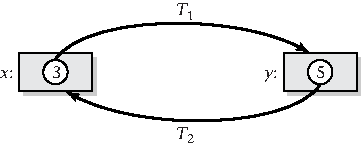
\includegraphics{hail_f0512}}
%\centerline{\epsfbox{scan-5-12.eps}}
\caption{If transactions release each read lock as soon as they are
  done reading the corresponding object, the execution may not be
  serializable.  For example, two transactions could swap $x$ and
  $y$'s values, as shown here.}
\label{scan-5-12}
\end{figure}
rather than making
the two equal.  In Exercise~\ref{relaxed-swap-exercise}, you can come up with a system history
exhibiting this phenomenon.

Other database systems, such as Oracle and PostgreSQL, take a more
radical approach to relaxed isolation, known as \vocab{multiversion
concurrency control} (\vocab{MVCC}).  Each write action stores the
new value for an entity in a different location than the old value.
Thus, a read action need not read the most recent version: it can read
an older version.  In particular, a transaction can read all entities
(other than those it has written itself) from the version that was
most recently committed when the transaction started.  Any writes
done since then by other transactions---whether committed or
otherwise---are completely ignored.  No read locks are needed at all.  This
is known as \foldvocab{snapshot}{isolation}.
When a transaction using snapshot isolation obtains a write lock and the entity being written was modified by some other transaction that committed since the writing transaction started, the write request is aborted with an error condition. The writing transaction must roll back and restart.

It should be clear that snapshot isolation provides repeatable reads.
Therefore, some people, forgetting that nonrepeatable reads are only
one symptom of relaxed isolation, think that snapshot isolation
suffices for serializability.  Regrettably, both Oracle and PostgreSQL
foster this belief by calling their snapshot isolation mode
``serializable.''  Neither offers true serializability, even as an option.
For example, on either of these systems, one transaction could copy
$x$ to $y$ while another was copying $y$ to $x$, even at the highest
isolation level.

\subsection{Coordinated Transaction Participants: Two-Phase Commit}
\label{two-phase-commit-section}
A transaction processing system can be built using the mechanisms I
have described thus far: two-phase locking and a write-ahead log
containing undo and redo entries.  However, you need one more mechanism
if you want to be able to coordinate multiple subsystems working
together on shared transactions.  That mechanism is the
\vocab{two-phase commit} protocol, which I describe in this section.
(Two-phase commit and two-phase locking
are unrelated, other than that each happens to contain two phases.)

As an example of coordination, a system might include both a
message-queuing system and a relational database.  Each uses the
mechanisms I have previously described in order to provide atomic and
durable transactions.  However, you would like to be able to have a
single transaction that first dequeues a request message from one
queue, then does some database operations, and finally writes a
response message into another queue.  All of this should be atomic and
durable, as a unit.  For example, if something goes wrong during
database processing, the rollback not only should undo any database
changes, but also should restore the request message to its queue.

Transaction processing systems generally
include a module specializing in this coordination, known as a \vocab{transaction manager}, as well as the various
\vocabs{resource manager}, such as message-queuing and database
systems.  The managers communicate with one another using the two-phase
commit protocol
in order to ensure that all
participants agree whether a transaction has aborted or committed.  In
particular, if the transaction commits, it must be durable in each
resource manager.

\index{Gray, Jim}Gray pointed out that the essence of two-phase commit is
the same as a wedding ceremony.  First, the officiating party asks all
the participants whether they really want to go ahead with the
commitment.  After each of them says ``I do,'' the officiating party
announces that the commitment has taken place.

In somewhat greater detail, the steps in the two-phase commitment
protocol are as follows, and as shown in Figure~\ref{scan-5-15}, for
\begin{figure}
\centerline{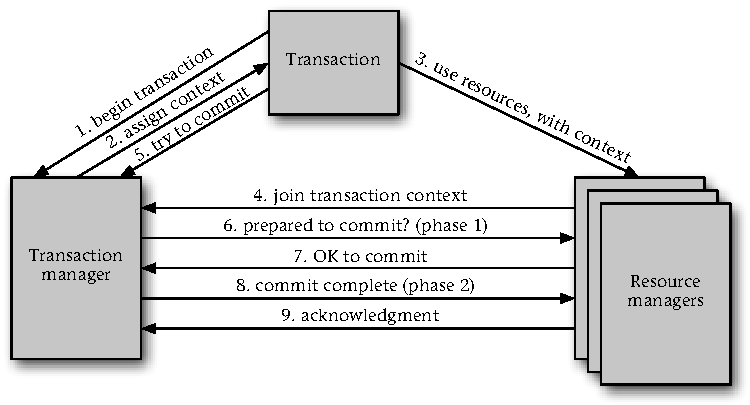
\includegraphics{hail_f0513}}
%\centerline{\epsfbox{scan-5-15.eps}}
\caption{The two-phase commit protocol coordinates transaction
  participants, as shown here and enumerated in the accompanying text.
  This diagram shows only the case in which all resource managers
  indicate that it is OK to commit, and so the transaction is committed.}
\label{scan-5-15}
\end{figure}
the case of a successful commitment:
\begin{enumerate}
\item
When a new transaction begins, it registers with the transaction
manager.
\item
In return, the transaction manager assigns an identifying \vocab{transaction context}.
\item
Whenever the transaction uses the services of a resource manager, it
presents its transaction context.  (If the resource manager
subcontracts to another resource manger, it passes the transaction
context along.)
\item
When a resource manager sees a new transaction context for the first
time, it registers with the transaction manager as being involved in
that transaction.  This is known as joining the transaction.
\item
When the transaction wishes to commit, it contacts the transaction
manager.
\item
The transaction manager knows all the involved resource
managers because of their earlier join messages.  The transaction
manager starts phase one by asking each of those resource managers
whether it is prepared to commit.
\item
When a resource manager is asked to prepare to commit, it checks
whether it has any reason not to.  (For example, a database system
might check whether any consistency constraints were violated.)  If
the resource manager detects a problem, it replies to the transaction
manager that the transaction should be aborted.  If there is no
problem, the resource manager first makes sure the transaction's
updates are all stored in persistent storage (for example, in redo log
records).  Then, once this is complete, the resource manager indicates
to the transaction manager that the transaction can commit, so far as
this resource manager is concerned.
\item
The transaction manager waits until it has received replies from all
the resource managers.  If the replies indicate unanimous agreement to
commit, the transaction manager logs a commitment record and notifies
all the resource managers, which starts phase two.
\item
When a resource manager hears that the transaction is in phase two of
commitment, it logs its own commit record and drops any exclusive
locks it has been holding for the transaction.  Once the transaction
is in phase two, there is no possibility it will abort and need to
perform undo actions.  Even if the system crashes and restarts, the transaction
manager will see its own commitment log record and go forward with
phase two.

Each resource manager then sends an acknowledgment to the transaction
manager, indicating completion of the phase two activity.  When all of
these acknowledgments are received, the transaction manager logs
completion of the commit.  That way, after a crash and restart, it
will know not to bother redoing phase two.
\end{enumerate}
On the other hand, if back in phase one the transaction manager hears
a request to abort from any resource manager or is forced to recover
after a crash and finds no commitment record, then it notifies the
resource managers to roll back the transaction, using their undo logs.

\section{Security and Transactions}\label{security-and-transactions-section}

Transaction processing systems are often used for an enterprise's
mission-critical operations.  As such, a great deal of thought has
gone into security issues in transaction processing systems.  However,
many of the issues that arise in these systems are not actually
particular to the transaction mechanism, per se.  Here I will
focus on security implications that stem from using atomic
transactions.

One security consequence of atomic transactions is salutary.  A system
constructed out of atomic transactions is much easier to reason about
than a more general system would be.  You saw in Chapter~\ref{synchronization-chapter} that
crackers can exploit race conditions, which would otherwise almost
never happen, in order to subvert a system's security design.  A
similar trick can be played by forcing a non-atomic operation to fail
after doing only some of its actions.  By using atomic transactions,
the system's designer excludes both of these entire categories of vulnerabilities.

Furthermore, security is enhanced by using a general-purpose
transaction processing infrastructure, rather than trying to achieve
atomicity through ad hoc means.  Nothing is more prone to
security vulnerabilities than complex code that is rarely used.  You
saw that achieving failure atomicity without a general mechanism, such
as the undo log, often involves considerable complex, nonmodular
code.  (For example, see
Exploration Project~\ref{kernel-failure-atomicity-exercise}, which
has you examine some Linux kernel source code.)  And yet, this messy,
bug-prone code is never tested under normal circumstances, because it
comes into play only in the case of a failure.  As such, bugs in it
could go undetected for years, until some cracker goes looking for
them.

By contrast, a general-purpose infrastructure (such as is included in
a reputable database system) has presumably been well tested, for two
reasons.  First, its correct operation is a central concern for its
authors, rather than peripheral.  Second, the exact same
infrastructure comes into play in all situations; for example, undo
logs are processed in deadlock recovery, user-initiated aborts, and
other failure situations.  As such, testing the mechanism in one
common situation provides some assurance of correct operation in
other, less common situations.

You have seen that one security guideline regarding transactions is simple:
they should be used.  Are there other, less simple and less positive interactions
between transactions and security?  Unfortunately, yes.  Transactions
are a very powerful abstraction mechanism; that is, they hide a great
deal of complexity behind a simple interface.  An application
programmer can think in terms of the simple interface and totally
ignore the complex underpinnings---except when those complex
underpinnings have security implications.  That is the great danger of
any abstraction mechanism, transactions included: it can blind you to
what is really going on.  Thus, another security guideline is to go beyond the
abstract view of transactions and consider the underlying mechanisms
discussed in this chapter.

One instance in which you need to think about transactions' underpinnings
occurs when you are reasoning about your system's vulnerability to denial of
service attacks.  Transaction processing systems do a great deal of
locking behind the scenes.  Generally, they provide not only deadlock
detection, but also timeouts on locks.  However, this doesn't mean
that a subverted transaction couldn't bring other transactions to
their knees.  Do you really want to wait the full timeout period for
each lock acquisition?

Worse, the usual way of handling locking
problems is to roll back the involved transactions and then restart
them. If the problems are caused by fluky coincidences, they will
almost surely not recur on the second try.  However, if your system is
being manipulated by a cracker, might you be put in the position of
repeatedly rolling back and retrying the same transactions?  If so,
you not only are making no headway, but also are consuming great
quantities of resources, such as processing time and log space.  After
how many retries should you give up?

Even aside from locking and
retries, you need to understand your transactions' consumption of log
space and other resources to be able to reason about denial of service
attacks.  Could an attacker trick you into filling up your log space
on disk?

Another pitfall would be to lose track of exactly what degree of
isolation your transactions enjoy relative to other concurrent
computations.  For example, suppose you have a transaction that
temporarily stores some confidential information into a widely
readable data entity, but then deletes the information before
committing.  (Alternatively, the transaction may store the information and then abort upon
discovering the information is confidential.)  Does
this suffice to protect the information from disclosure?  Maybe, maybe
not.  If your transaction is running in serializable isolation (that is,
with full two-phase locking), \emph{and so are all the concurrent
computations}, then the information is protected.  However, if you allow
an adversary to run transactions that don't acquire locks (for example,
SQL's ``read uncommitted'' isolation level), then you have not
protected the confidential information, no matter how serializable
your own transaction is and how careful it is to clean up all the data
before committing.

Similarly, suppose your transactions rely on keeping the database
consistent (maintaining invariant properties) in order to operate
correctly.  Specifically, if the database becomes inconsistent, your
transactions can be tricked into violating security policy.  Are you
safe if all the transactions have been declared to use the
``serializable'' isolation level, and adversaries are prevented from
introducing additional transactions?  Not necessarily.  As I
mentioned earlier, if you are using the Oracle or PostgreSQL database
system, the ``serializable'' isolation level doesn't actually provide
serializability; it provides only snapshot isolation.  If you don't
understand that, and exactly what snapshot isolation entails, you have
no way to reason about the kind of situations into which a cracker could
manipulate your transactions.  Perhaps the cracker could arrange
for your transactions to run in a nonserializable fashion that leaves
the database inconsistent in a way that creates a security
vulnerability.

Most transaction processing systems are closed environments, where
crackers cannot easily introduce extra transactions or even analyze
the existing transactions.  This makes them somewhat resistant to
attack.  Perhaps as a result, the risks mentioned here have generally
remained theoretical to date.  No known exploits take advantage of
programmers' confusion between snapshot isolation and true
serializability, for example.  Nonetheless, it is important to
remember that abstraction can be dangerous.  Unless you understand
what your system is really doing, you will not understand its
vulnerabilities.

One final pitfall for unwary programmers, with possible security
implications, is that a transaction manager can provide atomicity only 
for those actions under its control.  For example, throughout this
chapter, I have assumed that
transactions don't do any I/O.  Mature, full-featured transaction
processing systems also allow controlled I/O from transactions.  Until
a transaction commits, all its output is kept impounded.
Only upon commit is the output actually produced.  (Some systems go so
far as to use special I/O hardware that can be tested after a crash to
see whether the output was produced yet.)  In contrast to these
full-featured systems, many programmers build web-accessible
applications (in particular) with only a transactional database as
support.  In these systems, as in this textbook, I/O is not
automatically included in the transactional protection.  The
application programmer needs to take responsibility for not printing a
valuable ticket and then allowing the purchase to be aborted, for
example.

\section*{Exercises}
\begin{chapterEnumerate}
\item
\label{select-first}
In the example of deadlock detection and recovery in a database, each
of the two transactions tried to update two account balances, then
commit.  Suppose you add another step to the beginning of each
transaction: immediately before the first update, display the full
table, using \verb|select|.  Other than displaying the table, will
this have any impact on how the scenario plays out? Explain what will
happen if the transactions are executed in a system that is enforcing
serializability using two-phase locking.  (Note that this cannot be
tested using Oracle, because it uses MVCC, rather than two-phase locking.)
\item\label{t2-first-ex}
I introduced serial histories with an example where transaction $T_1$
added 3 to $x$ and $y$ and then transaction $T_2$ doubled $x$ and
$y$.  Write out the other serial history, in which $T_2$ comes first.
Leave the sequence of steps within each transaction the same as in the text,
but change the values appropriately.
\item\label{serializing-ex}
Prove that the example serializable history is equivalent to the
example serial history by showing the result of each
equivalence-preserving swap step along the way from the serializable
history to the serial history.
\item\label{reads-commute-ex}
For each of the following histories, if the
history is serializable, give an equivalent serial history.  Rather
than listing all the steps in the serial history, you can just list
the transaction numbers (1 and 2; or 1, 2, and 3) in the appropriate
order. If the history is not serializable, say so.
\begin{enumerate}
\item
$s_1(x), r_1(x), \overline{s}_1(x), e_1(z), w_1(z), \overline{e}_1(z), s_2(y), r_2(y),
  \overline{s}_2(y),$\\$e_2(x), w_2(x), \overline{e}_2(x), s_1(v), r_1(v), \overline{s}_1(v), e_1(y),
  w_1(y), \overline{e}_1(y)$
\item
$s_1(v),s_2(v),r_1(v), s_2(x), r_2(x), e_2(z), w_2(z), \overline{e}_2(z),\overline{s}_2(x),$\\$
  s_1(z), e_1(x), r_1(z), w_1(x), r_2(v), e_2(y),
  w_2(y),\overline{e}_1(x),\overline{s}_1(z),$\\$\overline{s}_1(v),\overline{s}_2(v),\overline{e}_2(y)$
\item
$s_1(x),s_1(y),s_2(x),s_2(z),s_3(y),s_3(z),r_1(x), r_2(x), r_2(z), r_3(z),$\\$r_3(y), r_1(y),\overline{s}_1(x),\overline{s}_1(y),\overline{s}_2(x),\overline{s}_2(z),\overline{s}_3(y),\overline{s}_3(z)$
\item
$e_1(x), w_1(x), \overline{e}_1(x), e_2(x), w_2(x), \overline{e}_2(x), e_2(z), w_2(z),
  \overline{e}_2(z),$\\$e_3(z), w_3(z), \overline{e}_3(z), e_3(y), w_3(y), \overline{e}_3(y), e_1(y),
  w_1(y), \overline{e}_1(y)$
\item
$e_1(x), r_1(x), s_2(y), r_2(y), \overline{s}_2(y), w_1(x), e_1(y), w_1(y),
  \overline{e}_1(y), \overline{e}_1(x),$\\$s_3(x), e_3(y),
  r_3(x), w_3(y), \overline{e}_3(y), \overline{s}_3(x)$
\end{enumerate}
\item
Of the serializable histories in
Exercise~\ref{reads-commute-ex}, which ones obey the two-phase locking rules?
\item\label{two-phase-orders-ex}
As an example of two-phase locking, page~\pageref{two-phase-examples} showed three different
two-phase histories for transaction $T_1$, which reads and writes $x$
and then reads and writes $y$.  Come up with at least five more
histories for this transaction that also obey the two-phase locking
rules.
\item\label{phase-two-purification-ex}
Explain why the rightmost phase two impurity of $T_j$ cannot conflict
with its right-hand neighbor.
\item
Explain why a pure transaction, $T_k$, with any of its actions
occurring as an impurity within the span of $T_j$ must lie entirely
within $T_j$'s phase one or entirely within $T_j$'s phase two.
\item
Some particular collections of transactions may not need two-phase
locking to ensure serializability.  However, this is generally a
fragile situation, which can be disturbed by the addition of another
transaction---even one obeying two-phase locking.
\begin{enumerate}
\item
Give two transaction histories, neither of which obeys the two-phase
locking rules, but which nonetheless always produce a serializable
system history, no matter how they are interleaved.
\item
Come up with a third transaction history, this one obeying two-phase
locking, such that when interleaved with the first two, a
nonserializable system history can result.
\end{enumerate}
\item\label{quadratic-undo-ex}
I mentioned that providing failure atomicity without an undo log
results in complex code.  For example, putting an explicit succession
of cleanup actions into each action's failure handling code can result in a
quadratic increase in code size.  Flesh out the details of this
argument by proving that if Figure~\ref{scan-5-9} on
page~\pageref{scan-5-9} were extended to include $n$ actions, it would
contain $\Theta(n^2)$ cleanup steps.
\item\label{reverse-chron-undo-ex}
Give an example of a transaction where it matters that undo log
entries are processed in reverse chronological order.
\item
\label{relaxed-swap-exercise}
Suppose you use relaxed-isolation locking rules, where shared locks are
held only for the duration of the read action and then are released
immediately afterward.  (Exclusive locks are still held until the end
of the transaction.)  Give a system history of two transactions, each
complying with these locking rules, in which one copies $x$'s value to $y$
and the other copies $y$'s value to $x$.  Starting with $x=3$ and
$y=5$, you should wind up with $x=5$ and $y=3$.
\item
Redo Exercise~\ref{select-first}, but instead of two-phase locking,
assume that the isolation level known as ``read
committed'' is used and is implemented with short read locks.  Then
do the exercise a third time, assuming snapshot isolation.  Only
the latter can be tested using Oracle.  (Oracle's read committed level
doesn't use short read locks.)  To test snapshot isolation using
Oracle, start each transaction with the following command:
\begin{verbatim}
set transaction isolation level serializable;
\end{verbatim}
\item
Suppose that when a stored value is increased by 1, an undo record
is written that does not include the old value.  Instead,
the undo record indicates that to undo the operation, the value should
be decreased by 1.  Is this idempotent?  What problems might arise
for crash recovery?
\item
On page~\pageref{two-phase-examples}, three example histories are given for the transaction $T_1$, each of which obeys two-phase locking.  Subsequently, page~\pageref{simple-two-phase} lists ``three very simple rules'' that suffice to ensure two-phase locking.  Do any of the three example histories obey those simple rules?  If so, which one(s)?
\item
The wording of page~\pageref{phase-one-definition}'s definitions of ``phase one'' and ``phase two'' (for two-phase locking) assumes that $T_j$ contains at least one unlock action.  Explain why this is a safe assumption, provided that $T_j$ contains any actions at all.
\item
Suppose $T_1$ writes new values into $x$ and $y$ and $T_2$ reads the values of both $x$ and $y$.  Is it possible for $T_2$ to see the old value of $x$ but the new value of $y$?  Answer this question three times: once assuming two-phase locking, once assuming the ``read committed'' isolation level is used and is implemented with short read locks, and once assuming snapshot isolation.  In each case, justify your answer.
\end{chapterEnumerate}

\section*{Programming Project}
\begin{chapterEnumerate}
\item
Build a simple, inefficient Java class to support transactions that
are atomic (under both concurrency and failure) but not durable, and
without deadlock detection.  The class should provide some state on which
the transactions can operate; for example, it might encapsulate an
array of integers, with \verb|put| and \verb|get| operations that the
transactions can use to modify and access slots within the array.  The
transactions need to limit themselves to this state, accessed through
these operations, in order to receive the guarantee of atomic
execution.

You can use Java's \verb|Thread|s as the transactions;
your class can find out which one is currently running using
\verb|Thread.currentThread()|.  Your class should take care of
automatically acquiring and releasing readers/writers locks (from
Programming Project \ref{rwlock-with-upgrade-exercise}),
in accordance with two-phase locking.  You will need to keep track
of the locks each transaction holds and an undo log for each transaction.
This per-transaction information can be stored using a \verb|Map| or using \verb|ThreadLocal| objects.

One design
option would be to provide three methods used to signal the start of a
transaction and its termination by commitment or abortion.  Another,
more object-oriented, option would be to encapsulate each transaction
using an interface analogous to \verb|Runnable| in the Java API, with
a \verb|run| method that carries out the whole transaction.  If that
method returns, the transaction commits; on the other hand, if the method throws
an exception, the transaction aborts.

As a client application for your class, you could write a program that
has multiple threads transferring money between bank accounts.  The
encapsulated array of integers could be used to store account
balances, with the array indexes serving as account numbers.
You should design the collection of concurrent transfers to be deadlock
free.  However, you should ensure that there are lots of
concurrent transfers and lots of cases where multiple transfers access
the same account.  That way, correct final balances provide good evidence
that your class was successful at warding off races.  Also, you
should include some transactions that abort after making updates,
so as to test the use of undo logs.

\end{chapterEnumerate}

\section*{Exploration Projects}
\begin{chapterEnumerate}
\item
Work through the examples in Chapter~25 (``Transactions'') of the
\textit{J2EE 1.4 Tutorial}.
\item
On a Linux system that uses an ext3fs file system, for which you have
permission to change mount options, experiment with the performance
impact of journaling options.  In particular, test a write-intensive
workload after mounting the file system with each of the options
\verb|data=journal|, \verb|data=ordered|, and
\verb|data=writeback|.  These control how much protection is
provided for file data (as opposed to metadata).  With the first, all
file operations are atomic and durable.  With the second, a crash may
occasionally leave data updated without the corresponding metadata
update.  With the third, it is even possible for metadata to be
updated but still be pointing at old data.  
Write a report 
carefully explaining what you did and in which hardware and software
system context you did it, so that someone else could replicate
your results.
\item
Carry out the scenario from Exercise~\ref{relaxed-swap-exercise} using a relational
database system.  You should use two interactive sessions, in each of
which you have given the command {\tt set transaction isolation level
read committed}.  Be sure to end your commands in each session with
{\tt commit} before  you inspect the outcome.
\item
Carry out the same scenario as in the previous project using Oracle
or PostgreSQL, with the {\tt transaction isolation level} set to
{\tt serializable}.
\item
Try the same scenario as in the previous project, using Microsoft SQL
Server or IBM DB2, with the {\tt transaction isolation level} set to
{\tt serializable}.  You should find that $x$ and $y$ are not swapped.  What
happens instead?  Does this depend on how you interleave the commands
in the two sessions?
\item
Come up with a plausible scenario where using snapshot isolation
rather than serializability results in a security vulnerability.  You
needn't show detailed SQL code, just an English description of what
the data would be and what the transactions would do with it.  (Some
more formality might be helpful, of course.)  Explain what an
adversary would need to do in order to exploit the vulnerability.
\item
\label{kernel-failure-atomicity-exercise}
The quadratic growth in code size in Exercise~\ref{quadratic-undo-ex} stems
from the assumption that each action's failure handler has its own disjoint
cleanup code.  This results in lots of repetitions of the same cleanup
actions.  One way to keep explicit per-action cleanup code (rather than a
general undo log) and yet avoid quadratic growth is to share the common
cleanup code, so that each cleanup action only appears once.  Failures later
in the transaction just execute more of that shared cleanup code than
failures earlier in the transaction do. An example of this pattern can
be found in the procedure \verb|copy_process| in the Linux kernel
source file \verb|kernel/fork.c|.  Skim this code (you don't need to
understand most of it) and write a description of what
programming language mechanism it uses to execute the appropriate
amount of cleanup code, based on how late the failure occurs.  Can you
think of an alternative programming language mechanism that could
serve the same purpose?  (This exercise was written when the kernel
was at version 2.6.0-test11; however, the relevant aspects of this
procedure seem to be stable across quite a few versions.)
\end{chapterEnumerate}

\section*{Notes}

My treatment of transactions barely scratches the surface.
If you are interested in transactions, you should read at
least one book devoted entirely to the topic.  The best to start with
is probably by \index{Bernstein, Philip A.}Bernstein and
\index{Newcomer, Eric}Newcomer~\cite{max1054}.  After that, you can
get a more detailed treatment of the underlying principles from
\index{Weikum, Gerhard}Weikum and \index{Vossen, Gottfried}Vossen~\cite{max1085}
or of the practical details (with lots of code) from 
\index{Gray, Jim}Gray and \index{Reuter, Andreas}Reuter~\cite{max1009}.

The earliest electronic transaction processing systems are poorly
documented in the open literature; apparently companies regarded
techniques for achieving atomicity and durability as proprietary.
(\index{Gray, Jim}Gray has suggested the developers merely prioritized code over
papers.)  Only in the mid- to late 1970s did techniques such as I
explain begin showing up in publications;
references \cite{max1005,max1007,max1050,max1004} still make good reading today.  A
longer, less polished work by Gray~\cite{max1056} was quite
influential; today, it is primarily of interest to historians, as much
of the same material appears in more polished form in his book with Reuter~\cite{max1009}.

\index{Harder, Theo@H{\"a}rder, Theo}H{\"a}rder and \index{Reuter,
Andreas}Reuter~\cite{max1001} introduced the acronym ACID.  In the
terminology I presented, isolation is subsumed under atomicity.  You
should be aware that some other authors instead treat atomicity as
meaning only atomicity in the face of failures.  \index{Lampson,
Butler W.}Lampson and \index{Sturgis, Howard E.}Sturgis~\cite{max1050}
use \vocab{unitary} to mean atomic with respect to failures; however,
this term does not seem to have caught on.

The specific
software versions used for the examples were Oracle Database 9i,
PostgreSQL~7.4, and J2EE~1.4.

I showed how workflow systems can be configured with message queues connecting the processing stages. A popular alternative is to connect each processing stage with a centralized process manager, which coordinates the workflow. For example,
upon receiving a message from order processing, the manager would send messages out to accounts receivable, shipping, and the customer. The process manager allows centralized monitoring and control. Process managers are sold as part of Enterprise Application Integration (EAI) products such as TIBCO's BusinessWorks.

I mentioned that my definitions of history, equivalence, and
serializability were chosen for simplicity and would not accommodate
more sophisticated concurrency control methods.  If you wish to pursue
this, the previously cited book by \index{Weikum, Gerhard}Weikum and
\index{Vossen, Gottfried}Vossen~\cite{max1085} provides a good
foundation.  Classic works on the topic include those by \index{Bernstein, Philip A.}Bernstein and
\index{Goodman, Nathan}Goodman~\cite{max1003,max1013} and by \index{Stearns, Richard
E.}Stearns and \index{Rosenkrantz, Daniel
J.}Rosenkrantz~\cite{max1014}.  Several works I will cite with regard
to relaxed isolation are also relevant here.

Two-phase locking seems to have first been published by
\index{Eswaran, K. P.@Eswaran, K.~P.}Eswaran et
al.~\cite{max1005}.  That same 1976 paper also brought to the fore a
difficult aspect of serializability in relational databases, which I
have glossed over.  Normally, locking is done at the granularity of
individual rows in database tables.  Suppose a transaction is
operating on all accounts with zero balances.  On the surface, you
might think it locks just those rows of the accounts table.  However, what
if a concurrent transaction is doing a withdrawal that brings another
account's balance down to zero?  Or inserting a new account with zero
balance?  This introduces the problem known as \vocabs{phantom}; a
transaction's assumptions can be invalidated not only by changes to
the rows the transaction has read, but also by the addition of new
rows.
Eswaran et al.'s proposed solution,
\foldvocabs{predicate}{lock}, was impractical if taken too literally
but provided the foundation for more practical techniques.

In describing durability and failure atomicity in the face of system
crashes, I differentiated volatile storage from persistent storage.
Real systems need to consider these issues in even greater detail.
For example, a system failure while overwriting a block on disk may
result in the disk having neither the old nor the new version
available.  This necessitates precautions, such as
writing two copies of critical blocks.  A good starting point
for this topic would be the works cited at the beginning of these
notes.

Key papers on snapshot isolation and other relaxations of isolation
include those by \index{Berenson, Hal}Berenson et
al.~\cite{max1022}; by \index{Kempster, Tim}Kempster,
\index{Stirling, Colin}Stirling, and \index{Thanisch,
Peter}Thanisch~\cite{max1023}; and by \index{Adya, Atul}Adya,
\index{Liskov, Barbara}Liskov, and
\index{O'Neil, Patrick E.}O'Neil~\cite{max1021}. Historically, the
original treatment of relaxed isolation was by \index{Gray, Jim}Gray
et al.~\cite{max1059}.

I attributed the wedding analogy for two-phase commit to \index{Gray,
Jim}Gray.  He seems to have first introduced it in a conference
paper~\cite{max1051} and then reused it in his book with
Reuter~\cite{max1009}.

Transactions are also being increasingly used in multi-threaded
programming as an alternative to the lock-based and lock-free
synchronization approaches illustrated in the previous chapter.  In
this context, the transactional objects are often as fine-grained as
individual memory locations, leading to the term \foldvocab{Transactional}{Memory} (\vocab{TM}).
This abstraction can either be supported in hardware (\foldvocab{Hardware}{Transactional Memory} or \vocab{HTM})
or in software (\foldvocab{Software}{Transactional Memory} or \vocab{STM}). The best survey of
the whole field is the book by \index{Harris, Tim}Harris, \index{Larus, James}Larus, and \index{Rajwar, Ravi}Rajwar~\cite{max1204}.
Although the practicality of STM has been questioned~\cite{max1206,max1207}, it seems promising, particularly when
embedded in a functional programming language such as \index{Haskell}Haskell~\cite{max1205} or \index{Clojure}Clojure.

%% This file is a portion of the source for Revised Edition 1.1 of
%% Operating Systems and Middleware: Supporting Controlled
%% Interaction, Copyright 2011 by Max Hailperin.  This work is
%% licensed under the Creative Commons Attribution-ShareAlike 3.0
%% Unported License. To view a copy of this license, visit
%% http://creativecommons.org/licenses/by-sa/3.0/ or send a letter to
%% Creative Commons, 171 Second Street, Suite 300, San Francisco,
%% California, 94105, USA.
\chapter{Virtual Memory}\label{vm-chapter}

\section{Introduction}
\label{vm-intro-section}

In Chapters \ref{synchronization-chapter} and \ref{transactions-chapter}, you have seen that synchronization
(including transactions) can control the interactions between
concurrent threads.  For example, synchronization can ensure that only
one thread at a time updates the memory locations holding a shared
data structure.  Now you will learn about another
form of control, which can provide each thread with its own private storage, rather than regulating the threads' access to shared
storage.

In this chapter, I will present a mechanism, \vocab{virtual memory},
that can be used to provide threads with private storage, thereby
controlling their interaction.  However, virtual memory turns out to
be a very general-purpose abstraction, useful for many goals other
than just giving threads some privacy.  Therefore, after using this
introductory section to present the basic concept of virtual memory,
I will devote Section~\ref{vm-uses-section} to surveying the applications of virtual
memory.  Only afterward will I turn to the details of mechanisms and
policies; you'll find the related discussions in Sections \ref{vm-reps} and \ref{vm-policies-section}.  The
chapter concludes with the standard features: security issues in
Section~\ref{vm-security-section}, then exercises, programming and
exploration projects, and notes. 

The essence of virtual memory is to decouple the addresses that
running programs use to identify objects from the addresses that the
memory uses to identify storage locations.  The former are known as
\foldvocabes{virtual}{address} and the latter as \foldvocabes{physical}{address}.  As background for understanding this distinction, consider first
a highly simplified diagram of a computer system, without virtual
memory, as shown in Figure~\ref{PM-diagram}.
\begin{figure}
\centerline{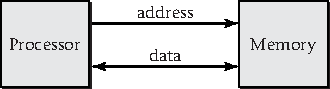
\includegraphics{hail_f0601}}
\iffalse
\centerline{\begin{graph}(252,72)
\graphnodesize{0}
\graphnodecolour{1}
\grapharrowlength{5}
\rectnode{P}[72,72](36,36)
\rectnode{M}[72,72](216,36)
\squarenode{PA}(72,54)
\squarenode{PD}(72,18)
\squarenode{MA}(180,54)
\squarenode{MD}(180,18)
\nodetext{P}{Processor}
\nodetext{M}{Memory}
\diredge{PA}{MA}
\diredge{MD}{PD}
\diredge{PD}{MD}
\bowtext{PA}{MA}{.06}{Address}
\bowtext{PD}{MD}{.06}{Data}
\end{graph}}
\fi
\caption{In a system without virtual memory, the processor sends addresses directly
  to the memory.}
\label{PM-diagram}
\end{figure}
In this system, the processor sends an address to the memory whenever
it wants to store a value into memory or load a value from memory.
The data being loaded or stored is also transferred in the appropriate
direction.  Each load operation retrieves the most recent value stored
with the specified address.  Even though the processor and
memory are using a common set of addresses to communicate, the role
played by addresses is somewhat different from the perspective of the
processor than from the perspective of the memory, as I will now
explain.

From the perspective of the processor (and the program the processor
is executing), addresses are a way of differentiating stored objects
from one another.  If the processor stores more than one value, and
then wishes to retrieve one of those values, it needs to specify which
one should be retrieved.  Hence, it uses addresses essentially as
names.  Just as an executive might tell a clerk to ``file this under
`widget suppliers'\,'' and then later ask the clerk to ``get me that
document we filed under `widget suppliers','' the processor tells the
memory to store a value with a particular address and then later
loads from that address.  Addresses used by executing programs to refer to objects are known as
\foldvocabes{virtual}{address}.

Of course, virtual addresses are not arbitrary names; each virtual address is a
number.  The processor may make use of this to give a group of related
objects related names, so that it can easily compute the name of any
object in the group.  The simplest example of this kind of grouping of
related objects is an array.  All the array elements are stored at
consecutive virtual addresses.  That allows the virtual address of any individual
element to be computed from the base virtual address of the array and the
element's position within the array.

From the memory's perspective, addresses are not identifying names for
objects, but rather are spatial locations of storage cells.  The
memory uses addresses to determine which cells to steer the data into
or out of. Addresses used by the memory
to specify storage locations are known as
\foldvocabes{physical}{address}.  Figure~\ref{scan-6-1} shows the
processor's and memory's views of addresses in a system like
that shown in Figure~\ref{PM-diagram}, where the physical addresses come directly from the virtual addresses, and so are numerically equal.
\begin{figure}
\centerline{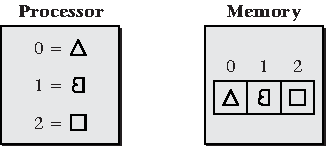
\includegraphics{hail_f0602}}
%\centerline{\epsfbox{scan-6-1.eps}}
\caption{In a system without virtual memory, virtual addresses (the
  processor's names for objects) equal physical addresses (the
  memory's storage locations).}
\label{scan-6-1}
\end{figure}

The difference between the processor's and memory's perspectives becomes apparent when you consider that
the processor may be dividing its time between multiple computational
processes.
Sometimes the processes will each need a private object,
yet the natural name to use will be the same in more than one process.
Figure~\ref{scan-6-2} shows how this necessitates using different
addresses in the processor and the memory.  That is, virtual addresses
can no longer be equal to physical addresses.
\begin{figure}
\centerline{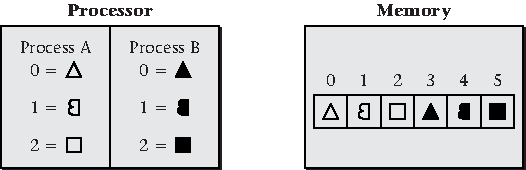
\includegraphics{hail_f0603}}
%\centerline{\epsfbox{scan-6-2.eps}}
\caption{When two processes each use the same virtual
  addresses as names for their own objects, the virtual addresses
  cannot equal the physical addresses, because each process's objects
  need to be stored separately.}
\label{scan-6-2}
\end{figure}
To make this work, general-purpose computers are
structured as shown in Figure~\ref{PMM-diagram}.
\begin{figure}
\centerline{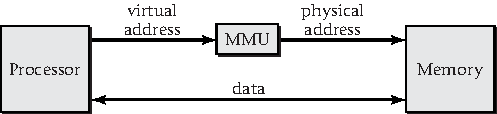
\includegraphics{hail_f0604}}
\iffalse
\centerline{\begin{graph}(312,83)
\graphnodesize{0}
\graphnodecolour{1}
\grapharrowlength{5}
\rectnode{P}[72,72](36,36)
\rectnode{M}[72,72](276,36)
\rectnode{MMU}[36,36](156,54)
\squarenode{PA}(72,54)
\squarenode{PD}(72,18)
\squarenode{MA}(240,54)
\squarenode{MD}(240,18)
\squarenode{MMUV}(138,54)
\squarenode{MMUP}(174,54)
\nodetext{P}{Processor}
\nodetext{M}{Memory}
\nodetext{MMU}{MMU}
\diredge{PA}{MMUV}
\diredge{MMUP}{MA}
\diredge{MD}{PD}
\diredge{PD}{MD}
\bowtext{PA}{MMUV}{.22}{\begin{tabular}{c}Virtual\\address\end{tabular}}
\bowtext{MMUP}{MA}{.22}{\begin{tabular}{c}Physical\\address\end{tabular}}
\bowtext{PD}{MD}{.04}{data}
\end{graph}}
\fi
\caption{The memory management unit (MMU) translates the processor's virtual
  addresses into the memory's physical addresses.}
\label{PMM-diagram}
\end{figure}
Program execution within the processor works entirely in terms of
virtual addresses.  However, when a load or store operation is
executed, the processor sends the virtual address to an intermediary,
the \vocab{memory management unit} (\vocab{MMU}).  The MMU translates
the virtual address into a corresponding physical address, which it
sends to the memory.

In Figure~\ref{scan-6-2}, each process uses the virtual address 0 as a
name for its own triangle.  This is a simplified model of how more complicated
objects are referenced by real processes.
Consider next a more realistic example of why each process might use the same
virtual addresses for its own objects.  Suppose several copies of the
same spreadsheet program are running.  Each copy will naturally want
to refer to ``the spreadsheet,'' but it should be a different
spreadsheet object in each process.  Even if each process uses a numerical name
(that is, a virtual address), it would be natural for all running instances of
the spreadsheet program to use the same address; after all, they are
running the same code.  Yet from the memory's perspective, the
different processes' objects need to be stored separately---hence, at
different physical addresses.

The same need for private names arises, if not quite so strongly, even
if the concurrent processes are running different programs.  Although in
principle each application program could use different names (that is,
virtual addresses) from all other programs, this requires a rather unwieldy
amount of coordination.

Even for shared objects, addresses as names behave somewhat
differently from addresses as locations.  Suppose two processes are
communicating via a shared bounded buffer; one is the producer, while
the other is the consumer.  From the perspective of one process, the
buffer is the ``output channel,'' whereas for the other process, it is
the ``input channel.''  Each process may have its own name for the
object; yet, the memory still needs to store the object in one location.
This holds true as well if the names used by the processes are numerical
virtual addresses.

Thus, once again, virtual addresses and physical
addresses should not be forced to be equal; it should be possible for
two processes to use the same virtual address to refer to different
physical addresses or to use different virtual addresses to refer to the
same physical address.

You have seen that the MMU maps virtual addresses to physical
addresses.  However, I have not yet discussed the nature of this mapping.  So
far as anything up to this point goes, the mapping could be as
simple as computing each physical address as twice the virtual
address.  However, that would not yield the very general mechanism
known as virtual memory.  Instead, virtual memory must have the following
additional properties:
\begin{itemize}
\item
The function that maps virtual addresses to physical addresses is
represented by a table, rather than by a computational rule (such as
doubling).  That way, the mapping can be much more general.
\item
However, to keep its size manageable, the table does not independently
list a physical address for each virtual address.  Instead, the
virtual addresses are grouped together into blocks known as
\vocabs{page}, and the table shows for each page of virtual addresses
the corresponding \vocab{page frame} of physical addresses.  I'll explain
this in greater detail in Section~\ref{vm-reps}.
In that same section, I also briefly
consider an alternative, \vocab{segmentation}.
\item
The contents of the table are controlled by the operating system.
This includes both incremental adjustments to the table (for purposes
you will see in Section~\ref{vm-uses-section}) and wholesale changes of the table
when switching between threads.  The latter allows each thread to have
its own private virtual address space, in which case, the threads belong to
different processes, as explained in Section~\ref{vm-private-storage-section}.
\item
The table need not contain a physical address translation for every
page of virtual addresses; in effect, some entries can be left blank.
These undefined virtual addresses are illegal for the processor to
use.  If the processor generates an illegal address, the MMU
interrupts the processor, transferring control to the operating
system.  This interrupt is known as a \vocab{page fault}.  This
mechanism serves not only to limit the usable addresses but also to
allow address translations to be inserted into the table only when
needed.  By creating address translations in this demand-driven fashion, many applications of virtual memory arrange to move data only when necessary,
thereby improving performance.
\item
As a refinement of the notion of illegal addresses, some entries in
the table may be marked as legal for use, but only in specific ways.  Most
commonly, it may be legal to read from some particular page of virtual
addresses but not to write into that page.  The main purpose this
serves is to allow trouble-free sharing of memory between processes.
\end{itemize}

In summary, then, virtual memory consists of an
operating system--defined table of mappings from virtual addresses to
physical addresses (at the granularity of pages), with the opportunity
for intervention by the operating system on accesses that the table
shows to be illegal.  You should be able to see that this is a very
flexible mechanism.  The operating system can switch between multiple
views of the physical memory.  Parts of physical memory may be
completely invisible in some views, because no virtual addresses map
to those physical addresses.  Other parts may be visible in more than
one view, but appearing at different virtual addresses.  Moreover, the
mappings between virtual and physical addresses need not be
established in advance.  By marking pages as illegal to access, and
then making them available when an interrupt indicates that they are
first accessed, the operating system can provide mappings on a
demand-driven basis.  In Section~\ref{vm-uses-section}, you will see several
uses to which this general mechanism can be put.

\section{Uses for Virtual Memory}\label{vm-uses-section}

This section contains a catalog of uses for virtual memory, one per subsection.
The applications of virtual memory enumerated are all
in everyday use in most general-purpose operating systems.  A
comprehensive list would be much longer and would include some
applications that have thus far been limited to research systems or
other esoteric settings.

\subsection{Private Storage}\label{vm-private-storage-section}

The introductory section of this chapter has already explained that each computation
running on a computer may want to have its own private storage,
independent of the other computations that happen to be running on the
same computer.  This goal of private storage can be further elaborated
into two subgoals:
\begin{itemize}
\item
Each computation should be able to use whatever virtual addresses it
finds most convenient for its objects, without needing to avoid using
the same address as some other computation.
\item
Each computation's objects should be protected from accidental (or
malicious) access by other computations.
\end{itemize}
Both subgoals---independent allocation and protection---can be
achieved by giving the computations their own virtual memory
mappings.  This forms the core of the process concept.

A \vocab{process} is a group of one or more threads with an associated
protection context.  I will introduce processes more fully in
Chapter~\ref{processes-chapter}.  In
particular, you will learn that the phrase ``protection context'' is
intentionally broad, including such protection features as file access permissions,
which you will study in Chapters \ref{processes-chapter} and \ref{persistence-chapter}.  For now, I will focus on
one particularly important part of a process's context: the mapping
of virtual addresses to physical addresses.  In other words, for the
purposes of this chapter, a process is a group of threads that share a virtual
address space.

As I will describe in Chapter~\ref{processes-chapter}, the computer hardware and
operating system software collaborate to achieve protection by
preventing any software outside the operating system from updating the
MMU's address mapping.  Thus, each process is restricted to accessing
only those physical memory locations that the operating system
has allocated as page frames for that process's pages.  Assuming that
the operating system allocates different processes disjoint portions
of physical memory, the processes will have no ability to interfere with one
another.  The physical memory areas for the processes need only
be disjoint at each moment in time; the processes can take
turns using the same physical memory.

This protection model, in which processes are given separate virtual
address spaces, is the mainstream approach today; for the purposes of
the present chapter, I will take it for granted.  In Chapter~\ref{processes-chapter}, I will also explore alternatives that allow all processes to
share a single address space and yet remain protected from one
another.

\subsection{Controlled Sharing}
\label{controlled-sharing-subsection}
Although the norm is for processes to use disjoint storage, sometimes
the operating system will map a limited portion of memory into more
than one process's address space.  This limited sharing may be a way
for the processes to communicate, or it may simply be a way to reduce
memory consumption and the time needed to initialize memory.  Regardless of the motivation, the shared physical
memory can occupy a different range of virtual addresses in each
process.  (If this flexibility is exercised, the shared memory should
not be used to store pointer-based structures, such as linked lists,
because pointers are represented as virtual addresses.)

The simplest example of memory-conserving sharing occurs when multiple
processes are running the same program.  Normally, each process divides
its virtual address space into two regions:
\begin{itemize}
\item
A read-only region holds the machine language instructions of the
program, as well as any read-only data the program contains, such as
the character strings printed for error messages.  This region is
conventionally called the \vocab{text} of the program.
\item
A read/write region holds the rest of the process's data.  (Many
systems actually use two read/write regions, one for the stack and one
for other data.)
\end{itemize}
All processes running the same program can share the same text.  The
operating system maps the text into each process's virtual memory address
space, with the protection bits in the MMU set to enforce read-only
access.  That way, the shared text does not accidentally become a
communication channel.

Modern programs make use of large libraries of supporting
code.  For example, there is a great deal of code related to graphical
user interfaces that can be shared among quite different programs,
such as a web browser and a spreadsheet.  Therefore, operating systems
allow processes to share these libraries with read-only protection,
just as for main programs.  Microsoft refers to shared libraries as
\vocabyies{dynamic-link librar} (\vocabs{DLL}).

Figure~\ref{scan-6-3} illustrates how processes can share in read-only
form both program text and the text of DLLs.  In this figure,
processes A and B are running program 1, which uses DLLs 1 and 2.
Processes C and D are running program 2, which uses DLLs 1 and 3.
Each process is shown as encompassing the appropriate program text,
DLLs, and writable data area.  In other words, each process encompasses
those areas mapped into its virtual address space.
\begin{figure}
\centerline{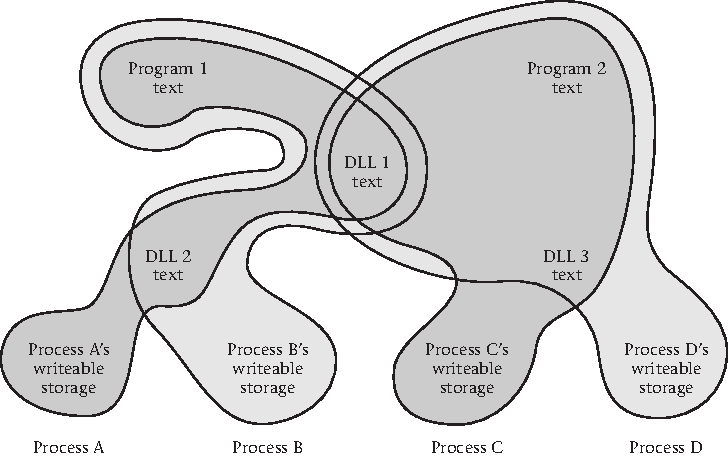
\includegraphics{hail_f0605}}
%\centerline{\epsfbox{scan-6-3.eps}}
\caption{The address space of a process includes the text of the
  program the process is running, the text of any DLLs used by that
  program, and a writable storage area for data.  Because processes A and B are
  both running program 1, which uses DLLs 1 and 2, their address
  spaces share these components.  Processes C and D are running
  program 2, which uses DLLs 1 and 3.  Because both programs use
  DLL~1, all four processes share it.}
\label{scan-6-3}
\end{figure}


From the operating system's perspective, the simplest way to support
interprocess communication is to map some physical memory into two
processes' virtual address spaces with full read/write permissions.
Then the processes can communicate freely; each
writes into the shared memory and reads what the other one writes.
Figure~\ref{scan-6-4} illustrates this sharing of a writable
area of memory for communication.
\begin{figure}
\centerline{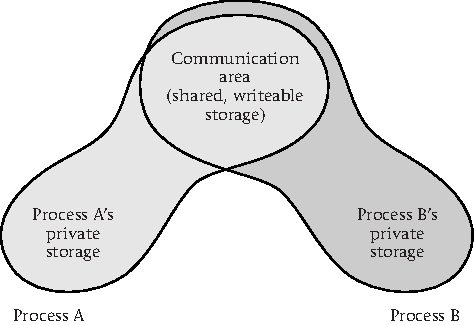
\includegraphics{hail_f0606}}
%\centerline{\epsfbox{scan-6-4.eps}}
\caption{Two processes can communicate by sharing a writable storage area.}
\label{scan-6-4}
\end{figure}

Simple as this may be for the operating system, it is anything but
simple for the application programmers.  They need to include mutexes,
readers-writers locks, or some similar synchronization structure in
the shared memory, and they need to take scrupulous care to use those
locks.  Otherwise, the communicating processes will exhibit races,
which are difficult to debug.

Therefore, some operating systems (such as Mac OS~X) use virtual
memory to support a more structured form of communication, known as
\vocab{message passing}, in which
one process writes a message into a block of memory and then asks the
operating system to send the message to the other process.  The
receiving process seems to get a copy of the sent message.  For small
messages, the operating system may literally copy the message from one
process's memory to the other's.  For efficiency, though, large
messages are not actually copied.  Instead, the operating system
updates the receiver's virtual memory map to point at the same
physical memory as the sender's message; thus, sender and receiver
both have access to the message, without it being copied.  To maintain
the ease of debugging that comes from message passing, the operating
system marks the page as read-only for both the sender and the
receiver.  Thus, they cannot engage in any nasty races.  Because the
sender composes the message before invoking the operating system, the
read-only protection is not yet in place during message composition
and so does not stand in the way.

As a final refinement to message passing by read-only sharing, systems
such as Mac OS~X offer \vocab{copy on write} (\vocab{COW}).  If either
process tries to write into the shared page, the MMU will use an
interrupt to transfer control to the operating system.  The operating
system can then make a copy of the page, so that the sender and
receiver now have their own individual copies, which can be
writable.  The operating system resumes the process that was trying
to write, allowing it to now succeed.  This provides the complete
illusion that the page was copied at the time the message was sent, as
shown in Figure~\ref{scan-6-5}.
\begin{figure}
\centerline{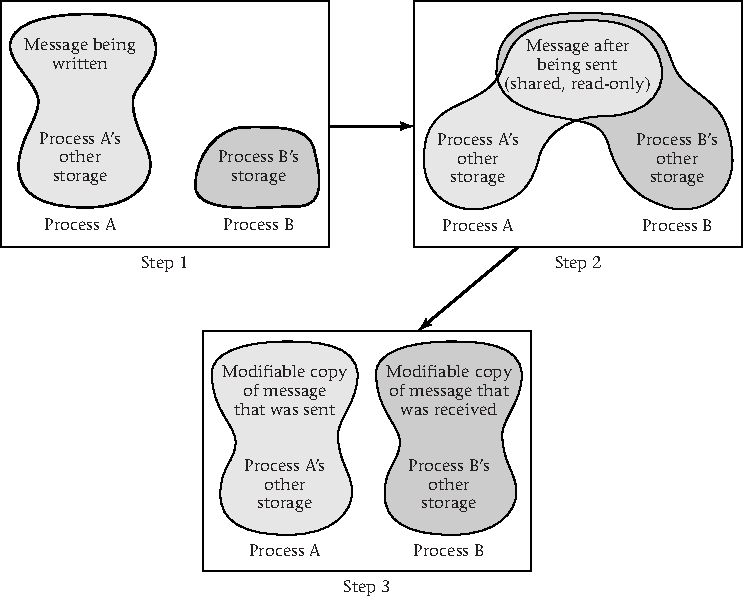
\includegraphics{hail_f0607}}
%\centerline{\epsfbox{scan-6-5.eps}}
\caption{To use copy on write (COW) message passing, process~A
  writes a message into part of its private memory (Step~1) and then
  asks the operating system to map the memory containing the message into process~B's
  address space as well (Step~2).  Neither process has permission to write into
  the shared area.  If either violates this restriction, the operating
  system copies the affected page, gives each process write
  permission for its own copy, and allows the write operation to
  proceed (Step~3).  The net effect is the same as if the message were copied
  when it was sent, but the copying is avoided if neither process writes into
  the shared area.}
\label{scan-6-5}
\end{figure}
The advantage is that if the processes do not write into most message pages, most
of the copying is avoided.

\subsection{Flexible Memory Allocation}

The operating system needs to divide the computer's memory among
the various processes, as well as retain some for its own use.
At first glance, this memory allocation problem doesn't seem too
difficult.  If one process needs 8 megabytes (MB) and another needs
10, the operating system could allocate the first 8~MB of
the memory (with the lowest physical addresses) to the first process
and the next 10~MB to the second.  However, this kind of
contiguous allocation runs into two difficulties.

The first problem with contiguous allocation is that the amount of
memory that each process requires may grow and shrink as the program
runs.  If the first process is immediately followed in memory by the
second process, what happens if the first process needs more space?

The second problem with contiguous allocation is that processes exit,
and new processes (with different sizes) are started.  Suppose you have
512~MB of memory available and three processes running, of sizes
128~MB, 256~MB, and 128~MB.  Now suppose the first and third processes
terminate, freeing up their 128-MB chunks of memory.  Suppose a 256-MB
process now starts running.  There is enough memory available, but not
all in one contiguous chunk, as illustrated in Figure~\ref{scan-6-6}.
\begin{figure}
\centerline{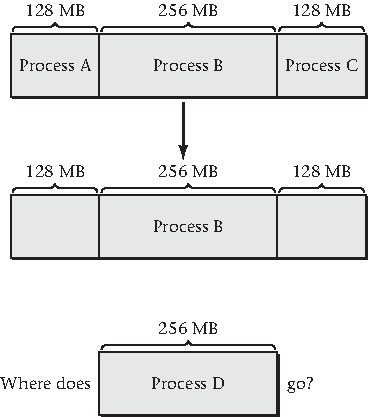
\includegraphics{hail_f0608}}
%\centerline{\epsfbox{scan-6-6.eps}}
\caption{Contiguous allocation leads to external fragmentation.  In
  this example, there is no contiguous 256-MB space available for
  process~D, even though the termination of processes A and C has
  freed up a total of 256~MB.}
\label{scan-6-6}
\end{figure}
This situation is known as \foldvocab{external}{fragmentation}.  I
will discuss external fragmentation more carefully in
Chapter~\ref{persistence-chapter}, because contiguous allocation is
important for disk space.  (I will also define the contrasting term,
internal fragmentation, in that same chapter.)

Because all modern general-purpose systems have virtual memory, these
contiguous allocation difficulties are a non-issue for main memory.
The operating system can allocate any available physical page frames
to a process, independent of where they are located in memory. 
For example, the conundrum of
Figure~\ref{scan-6-6} could be solved as shown in
Figure~\ref{discontiguous}.
\begin{figure}
\centerline{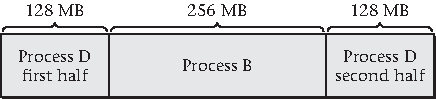
\includegraphics{hail_f0609}}
%\centerline{\epsfbox{discontiguous.eps}}
\caption{With virtual memory, the physical memory allocated to a
  process need not be contiguous, so process~D can be accommodated even
  without sufficient memory in any one place.}
\label{discontiguous}
\end{figure}
In a more realistic setting, it would be
surprising for the pattern of physical memory allocation to display
even this degree of contiguity.  However, the
virtual addresses can be contiguous even if the physical addresses
are scattered all over the memory. 

\subsection{Sparse Address Spaces}

Just as virtual memory provides the operating system with flexibility
in allocating physical memory space, it provides each application
program (or process) with flexibility in allocating virtual address
space.  A process can use whatever addresses make sense for its data
structures, even if there are large gaps between them.  This provides
flexibility for the compiler and runtime environment, which assign
addresses to the data structures.

Suppose, for example, that a process has three data structures (S1, S2, and
S3) that it needs to store.  Each needs to be allocated in a
contiguous range of addresses, and each needs to be able to grow at
its upper end.  The picture might look like this, with addresses in megabytes:
\[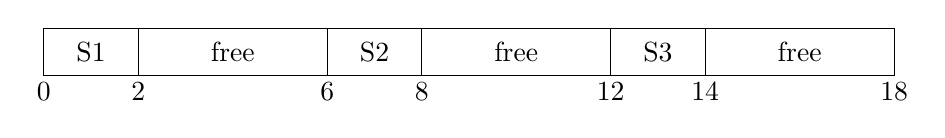
\begin{tikzpicture}[scale=.03]
\draw (0,0) rectangle (40,20);
\draw (40,0) rectangle (120,20);
\draw (120,0) rectangle (160,20);
\draw (160,0) rectangle (240,20);
\draw (240,0) rectangle (280,20);
\draw (280,0) rectangle (360,20);
\draw (20,10) node{S1};
\draw (80,10) node{free};
\draw (140,10) node{S2};
\draw (200,10) node{free};
\draw (260,10) node{S3};
\draw (320,10) node{free};
\draw (0,-7) node{0};
\draw (40,-7) node{2};
\draw (120,-7) node{6};
\draw (160,-7) node{8};
\draw (240,-7) node{12};
\draw (280,-7) node{14};
\draw (360,-7) node{18};
\end{tikzpicture}\]
\iffalse
\[\begin{graph}(370,32)(-3,-12)
\graphlinecolour{0}
\fillednodesfalse
\rectnode{a}[40,20](20,10)
\rectnode{b}[80,20](80,10)
\rectnode{c}[40,20](140,10)
\rectnode{d}[80,20](200,10)
\rectnode{e}[40,20](260,10)
\rectnode{f}[80,20](320,10)
\autonodetext{a}{S1}
\autonodetext{b}{free}
\autonodetext{c}{S2}
\autonodetext{d}{free}
\autonodetext{e}{S3}
\autonodetext{f}{free}
\freetext(0,-7){0}
\freetext(40,-7){2}
\freetext(120,-7){6}
\freetext(160,-7){8}
\freetext(240,-7){12}
\freetext(280,-7){14}
\freetext(360,-7){18}
\end{graph}\]
\fi
In this example, only one third of the 18-MB address range is actually
occupied.  If you wanted to allow each structure to grow more, you would
have to position them further apart and wind up with an even lower
percentage of occupancy.  Many real processes span an address range of
several gigabytes without using anywhere near that much storage.
(Typically, this is done to allow one region to grow up from the
bottom of the address space and another to grow down from the top.)

In order to allow processes to use this kind of
\foldvocab{sparse}{address space} without wastefully occupying a
corresponding amount of physical memory, the operating system simply
doesn't provide physical address mappings for virtual addresses in the
gaps.

\subsection{Persistence}

Any general-purpose operating system must provide some way for users
to retain important data even if the system is shut down and
restarted.  Most commonly, the data is kept in files, although other
kinds of persistent objects can be used.  The persistent objects are
normally stored on disk. For example, as I write this book, I am
storing it in files on disk.  That way, I don't have to retype the
whole book every time the computer is rebooted.  I will consider
persistence in more detail in Chapter~\ref{persistence-chapter}; for
now, the only question is how it relates to virtual memory.

When a process needs to access a file (or other persistent object),
it can ask the operating system to map the file into its address
space.  The operating system doesn't actually have to read the whole
file into memory.  Instead, it can do the reading on a demand-driven
basis.  Whenever the process accesses a particular page of the file
for the first time, the MMU signals a page fault.  The operating
system can respond by reading that page of the file into memory,
updating the mapping information, and resuming the process. (For
efficiency reasons, the operating system might choose to fetch
additional pages at the same time, on the assumption they are likely
to be needed soon.  I discuss this possibility in Section~\ref{fetch-policy}.)

If the process writes into any page that
is part of a mapped file, the operating system must remember to write
the page back to disk, in order to achieve persistence.  For efficiency, the
operating system should not write back pages that have not been
modified since they were last written back or since they were read in.
This implies the operating system needs to know which pages have been
modified and hence are not up to date on disk.  (These are called
\vocab{dirty} pages.)

One way to keep track of dirty pages, using only techniques I have
already discussed, is by initially marking all pages read-only.  That
way, the MMU will generate an interrupt on the first attempt to write
into a clean page.  The operating system can then make the page
writable, add it to a list of dirty pages, and allow the operation to
continue.  When the operating system makes the page clean again, by
writing it to disk, it can again mark the page read-only.

Because keeping track of dirty pages is such a common requirement and
would be rather inefficient using the approach just described, MMUs
generally provide a more direct approach.  In this approach, the MMU keeps a
\vocab{dirty bit} for each page.  Any write into the page causes the
hardware to set the dirty bit without needing operating system
intervention.  The operating system can later read the dirty bits and
reset them.  (The Intel Itanium architecture contains a compromise:
the operating system sets the dirty bits, but with some hardware
support.  This provides the flexibility of the software approach
without incurring so large a performance cost.)

\subsection{Demand-Driven Program Loading}

One particularly important case in which a file gets mapped into memory is
running a program.  Each executable program is ordinarily stored as a
file on disk.  Conceptually, running a program consists of reading the
program into memory from disk and then jumping to the first
instruction.

However, many programs are huge and contain parts that may not always
be used.  For example, error handling routines will get used only if
the corresponding errors occur.  In addition, programs often support more
features and optional modes than any one user will ever need.  Thus,
reading in the whole program is quite inefficient.

Even in the rare case that the whole program gets used, an interactive
user might prefer several short pauses for disk access to one long
one.  In particular, reading in the whole program initially means that
the program will be slow to start, which is frustrating.  By reading
in the program incrementally, the operating system can start it
quickly at the expense of brief pauses during operation.  If each of
those pauses is only a few tens of milliseconds in duration and
occurs at the time of a user interaction, each will be below the
threshold of human perception.

In summary, operating system designers have two reasons to use virtual memory
techniques to read in each program on a demand-driven basis: in order to avoid
reading unused portions and in order to quickly start the program's execution.  As with more general
persistent storage, each page fault causes the operating system to
read in more of the program.

One result of demand-driven program loading is that application programmers can make their
programs start up more quickly by grouping all the necessary code together
on a few pages. Of
course, laying out the program text is really not a job for the
human application programmer, but for the compiler and linker.
Nonetheless, the programmer may be able to provide some guidance to these tools.

\subsection{Efficient Zero Filling}

For security reasons, as well as for ease of debugging, the operating
system should never let a process read from any memory location that
contains a value left behind by some other process that previously
used the memory.  Thus, any memory not occupied by a persistent
object should be cleared out by the operating system before a new process accesses it.

Even this seemingly mundane job---filling a region of memory with
zeros---benefits from virtual memory.  The operating system can fill
an arbitrarily large amount of virtual address space with zeros using
only a single zeroed-out page frame of physical memory.  All it needs
to do is map all the virtual pages to the same physical page frame
and mark them as read-only.

In itself, this technique of sharing a page frame of zeros
doesn't address the situation where a process writes into one of its
zeroed pages.  However, that situation can be handled using a variant of the COW technique
mentioned in Section~\ref{controlled-sharing-subsection}.  When the MMU
interrupts the processor due to a write into the read-only page of
zeros, the operating system can update the mapping for that one page
to refer to a separate read/write page frame of zeros and then resume the
process.

If it followed the COW principle literally, the operating system would
copy the read-only page frame of zeros to produce the separate,
writable page frame of zeros.  However, the operating system can run faster
by directly writing zeros into the new page frame without needing to
copy them out of the read-only page frame. In fact, there is no
need to do the zero filling only on demand.  Instead, the operating
system can keep some spare page frames of zeros around, replenishing
the stock during idle time.  That way, when a page fault occurs from
writing into a read-only page of zeros, the operating system can simply
adjust the address map to refer to one of the spare prezeroed page
frames and then make it writable.

When the operating system proactively fills spare page frames with zeros
during idle time, it should bypass the processor's normal cache memory
and write directly into main memory.  Otherwise, zero filling can
seriously hurt performance by displacing valuable data from the cache.

\subsection{Substituting Disk Storage for RAM}
\label{disk-for-RAM}
In explaining the application of virtual memory to persistence, I
showed that the operating system can read accessed pages into memory
from disk and can write dirty pages back out to disk.  The reason for
doing so is that disk storage has different properties from main
semiconductor memory (RAM).  In the case of persistence, the relevant
difference is that disk storage is nonvolatile; that is, it retains its
contents without power.  However, disk differs from RAM in other
regards as well.  In particular, it is a couple orders of magnitude
cheaper per gigabyte.  This motivates another use of virtual memory,
where the goal is to simulate having lots of RAM using less-expensive
disk space.  Of course, disk is also five orders of magnitude slower
than RAM, so this approach is not without its pitfalls.

Many processes have long periods when they are not actively running.
For example, on a desktop system, a user may have several applications
in different windows---a word processor, a web browser, a mail reader,
a spreadsheet---but focus attention on only one of them for minutes or
hours at a time, leaving the others idle.  Similarly, within a
process, there may be parts that remain inactive.  A spreadsheet user
might look at the online help once, and then not again during several
days of spreadsheet use.

This phenomenon of inactivity provides an opportunity to capitalize on
inexpensive disk storage while still retaining most of the
performance of fast semiconductor memory.  The computer system needs
to have enough RAM to hold the \vocab{working set}---the active
portions of all active processes.  Otherwise, the performance will be
intolerably slow, because of disk accesses made on a routine basis.  However,
the computer need not have enough RAM for the entire storage needs of
all the processes: the inactive portions can be shuffled off to disk,
to be paged back in when and if they again become active.  This will
incur some delays for disk access when the mix of activity changes,
such as when a user sets the word processor aside and uses a spreadsheet
for the first time in days.  However, once the new working set of
active pages is back in RAM, the computer will again be as responsive
as ever.

Much of the history of virtual memory focuses on this one application,
dating back to the invention of virtual memory in the early 1960s.
(At that time, the two memories were magnetic cores and magnetic drum,
rather than semiconductor RAM and magnetic disk.)  Even though this
kind of paging to disk has become only one of many roles played by
virtual memory, I will still pay it considerable attention.  In particular,
some of the most interesting policy questions arise only for this
application of virtual memory.  When the operating system needs to
free up space in overcrowded RAM, it needs to guess which pages are
unlikely to be accessed soon. I will come back to this topic
(so-called replacement policies) after first considering other
questions of mechanism and policy that apply across the full spectrum
of virtual memory applications.

\section{Mechanisms for Virtual Memory}
\label{vm-reps}

Address mapping needs to be flexible, yet efficient. As I mentioned
in Section~\ref{vm-intro-section}, this means that the mapping function is stored in an explicit
table, but at the granularity of pages rather than individual bytes or
words.  Many systems today use fixed-size pages, perhaps with a few
exceptions for the operating system itself or hardware access, though
research suggests that more general mixing of page sizes can be
beneficial.  (As explained in the notes, Linux has moved in this direction.)

Typical page sizes have grown over the decades, for reasons you can
explore in Exercises \ref{page-size-execercise-1} and \ref{page-size-execercise-2}; today, the most common
is 4 kilobytes (KB).  Each page of virtual memory and each page frame of physical
memory is this size, and each starts at an address that is a multiple
of the page size.  For example, with 4-KB pages, the first page (or
page frame) has address 0, the next has address 4096, then 8192, and
so forth.

Each page of virtual memory address space maps to an underlying page
frame of physical memory or to none. For example,
Figure~\ref{example-mapping} shows one possible mapping, on a system
with unrealistically few pages and page frames.
\begin{figure}
\centerline{\includegraphics{hail_f0610}}
\iffalse
\centerline{\begin{graph}(100,200)
\graphlinecolour{0}
\grapharrowlength{5}
\fillednodesfalse
\graphnodesize{20}
\squarenode{p0}(20,150)
\squarenode{p1}(20,130)
\squarenode{p2}(20,110)
\squarenode{p3}(20,90)
\squarenode{p4}(20,70)
\squarenode{p5}(20,50)
\squarenode{p6}(20,30)
\squarenode{p7}(20,10)
\squarenode{f0}(100,110)
\squarenode{f1}(100,90)
\squarenode{f2}(100,70)
\squarenode{f3}(100,50)
\textnode{x2}(50,110){X}[\graphlinewidth{0}\graphlinecolour{1}]
\textnode{x3}(50,90){X}[\graphlinewidth{0}\graphlinecolour{1}]
\textnode{x4}(50,70){X}[\graphlinewidth{0}\graphlinecolour{1}]
\textnode{x5}(50,50){X}[\graphlinewidth{0}\graphlinecolour{1}]
\textnode{x7}(50,10){X}[\graphlinewidth{0}\graphlinecolour{1}]
\autonodetext{p0}[w]{0}
\autonodetext{p1}[w]{1}
\autonodetext{p2}[w]{2}
\autonodetext{p3}[w]{3}
\autonodetext{p4}[w]{4}
\autonodetext{p5}[w]{5}
\autonodetext{p6}[w]{6}
\autonodetext{p7}[w]{7}
\autonodetext{f0}[e]{0}
\autonodetext{f1}[e]{1}
\autonodetext{f2}[e]{2}
\autonodetext{f3}[e]{3}
\diredge{p0}{f1}
\diredge{p1}{f0}
\diredge{p2}{x2}
\diredge{p3}{x3}
\diredge{p4}{x4}
\diredge{p5}{x5}
\diredge{p6}{f3}
\diredge{p7}{x7}
\freetext(20,170){Pages}
\freetext(100,130){Page frames}
\end{graph}}
\fi
\caption{In this example mapping of eight pages to four page frames,
  page~0 has been allocated page frame~1, page~1 has been allocated
  page frame~0, and page~6 has been allocated page frame~3.  The Xs
  indicate that no page frame is assigned to hold pages 2--5 or
  page 7.  Page frame~2 is unused.}
\label{example-mapping}
\end{figure}
The numbers next to the
boxes are page numbers and page frame numbers.  The starting
addresses are these numbers multiplied by the page size.
At the top of this figure, you can see that page~0 is stored in page
frame~1.  If the page size is 4~KB, this means that virtual address 0
translates to physical address 4096, virtual address 100 translates to
physical address 4196, and so forth.  The virtual address of the last
4-byte word in
page~0, 4092, translates to the physical address of the last word in page frame~1,
8188.  Up until this point, all physical addresses were found by
adding 4096 to the virtual address.  However, the very next virtual
address, 4096, translates to physical address 0, because it starts a
new page, which is mapped differently.  Note also that page frame~2 is
currently not holding any page, and that pages 2--5 and page~7 have no
translation available.  In
Exercise~\ref{page-6-translation-exercise}, you can gain experience working with this
translation of virtual addresses into physical addresses by
translating the addresses for page~6.

Of course, a realistic computer system will have many more page frames
of physical memory and pages of virtual address space.  Often there
are tens or hundreds of thousands of page frames and at least
hundreds of thousands of pages.  As a result, operating system
designers need to think carefully about the data structure used to
store the table that maps virtual page numbers to physical page frame
numbers.  Sections \ref{linear-page-tables-section} through \ref{hashed-page-tables-section} will be devoted to presenting three
alternative structures that are in current use for page tables:
linear, multilevel, and hashed.  (Other alternatives that have fallen
out of favor, or have not yet been deployed, are briefly mentioned in
the end-of-chapter notes.)

Whatever data structure the operating system uses for its page table,
it will need to communicate the mapping information to the hardware's
MMU, which actually performs the mapping.  The nature of this
software/hardware interface constrains the page table design and also
provides important context for comparing the performance of
alternative page table structures.  Therefore, in
Section~\ref{vm-hw-sw-interface}, I will explain the two
forms the software/hardware interface can take.

Finally, Section~\ref{vm-segmentation-section} provides a brief look at segmentation, which was
historically important both as an alternative to paging and as an
adjunct to it.

\subsection{Software/Hardware Interface}\label{vm-hw-sw-interface}

You have seen that the operating system stores some form of page table
data structure in memory, showing which physical memory page frame (if
any) holds each virtual memory page.  Although I will present
several possible page table structures shortly, the most important
design issue applies equally to all of them: the page table should
almost never be used.

Performance considerations explain why such an important data
structure should be nearly useless (in the literal sense).  Every
single memory access performed by the processor generates a virtual
address that needs translation to a physical address.  Naively, this
would mean that every single memory access from the processor requires
a lookup operation in the page table.  Performing that lookup
operation would require at least one more memory access, even if the
page table were represented very efficiently.  Thus, the number of
memory accesses would at least double: for each real access, there
would be one page table access.  Because memory performance is often the
bottleneck in modern computer systems, this means that virtual memory
might well make programs run half as fast---unless the page table
lookup can be mostly avoided.  Luckily, it can.

The virtual addresses accessed by realistic software are not random;
instead, they exhibit both \foldvocab{temporal}{locality} and \foldvocab{spatial}{locality}.
That is, addresses that are accessed once are likely to be accessed
again before long, and nearby addresses are also likely to be accessed
soon.  Because a nearby address is likely to be on the same page, both
kinds of locality wind up creating temporal locality when considered
at the level of whole pages.  If a page is accessed, chances are good
that the same page will be accessed again soon, whether for the same
address or another.

The MMU takes advantage of this locality by keeping a
quickly accessible copy of a modest number of recently used
virtual-to-physical translations.  That is, it stores a limited number
of pairs, each with one page number and the corresponding page frame
number.  This collection of pairs is called the \vocab{translation
lookaside buffer} (\vocab{TLB}).  Most memory accesses will refer to
page numbers present in the TLB, and so the MMU will be able to
produce the corresponding page frame number without needing to access
the page table.  This happy circumstance is known as a \foldvocab{TLB}{hit}; the
less fortunate case, where the TLB does not contain the needed
translation, is a \foldvocab{TLB}{miss}.

The TLB is one of the most performance-critical components of a modern
microprocessor.  In order for the system to have a fast clock cycle
time and perform well on small benchmarks, the TLB must be very
quickly accessible.  In order for the system's performance not to fall
off sharply on larger workloads, the TLB must be reasonably large
(perhaps hundreds of entries), so that it can still prevent most page
table accesses.  Unfortunately, these two goals are in conflict with
one another: chip designers know how to make lookup tables large or
fast, but not both.  Coping as well as possible with this dilemma
requires cooperation from the designers of hardware, operating system,
and application software:
\begin{itemize}
\item
The hardware designers ameliorate the problem by including
{\em two} TLBs, one for instruction fetches and one for data loads
and stores.  That way, these two categories of memory access don't
need to compete for the same TLB.
\item
The hardware designers may further ameliorate the problem by including
a hierarchy of TLBs, analogous to the cache hierarchy.  A small, fast
level-one (L1) TLB makes most accesses fast, while a larger,
slower level-two (L2) TLB ensures that the page table won't need to be
accessed every time the L1 TLB misses.  As an example, the AMD Opteron
microprocessor contains 40-entry L1 instruction and data TLBs,
and it also contains 512-entry L2 instruction and data TLBs.
\item
The hardware designers also give the operating system designers some
tools for reducing the demand for TLB entries.  For example, if
different TLB entries can provide mappings for pages of varying sizes,
the operating system will be able to map large, contiguously allocated
structures with fewer TLB entries, while still retaining flexible
allocation for the rest of virtual memory.
\item
The operating system designers need to use tools such as variable page
size to reduce TLB entry consumption.  At a minimum, even if all
application processes use small pages (4~KB), the operating system
itself can use larger pages.  Similarly, a video frame buffer of many
consecutive megabytes needn't be carved up into 4-KB chunks.  As a
secondary benefit, using larger pages can reduce the size of page tables.
In many cases, smaller page tables are also quicker to access.
\item
More fundamentally, all operating system design decisions need to be
made with an eye to how they will affect TLB pressure, because this is
such a critical performance factor.  One obvious example is the normal
page size.  Another, less obvious, example is the size of the
scheduler's time slices: switching processes frequently will increase
TLB pressure and thereby hurt performance, even if the TLB doesn't need
to be flushed at every process switch. (I will take up that latter
issue shortly.)
\item
The application programmers also have a role to play.  Programs that
exhibit strong locality of reference will perform much better, not
only because of the cache hierarchy, but also because of the TLB.  The
performance drop-off when your program exceeds the TLB's capacity is
generally quite precipitous.  Some data structures are inherently more
TLB-friendly than others.  For example, a large,
sparsely occupied table may perform much worse than a smaller, more
densely occupied table.  In this regard, theoretical analyses of
algorithms may be misleading, if they assume all memory operations
take a constant amount of time.
\end{itemize}

At this point, you have seen that each computer system uses two
different representations of virtual memory mappings: a page table and
a TLB.  The page table is a comprehensive but slow representation,
whereas the TLB is a selective but fast representation.  You still need
to learn how entries from the page table get loaded into the TLB.  This
leads to the topic of the software/hardware interface.

In general, the MMU loads page table entries into the TLB on a
demand-driven basis.  That is, when a memory access results in a TLB
miss, the MMU loads the relevant translation into the TLB from the
page table, so that future accesses to the same page can be TLB hits.
The key difference between computer architectures is whether the MMU
does this TLB loading autonomously, or whether it does it with lots of
help from operating system software running on the processor.

In many architectures, the MMU contains hardware, known as a \foldvocab{page
table}{walker}, that can do the page table lookup operation without
software intervention.  In this case, the operating system must
maintain the page table in a fixed format that the hardware
understands.  For example, on an IA-32 processor (such as the
Pentium~4), the operating system has no other realistic option than to
use a multilevel page table, because the hardware page table walker
expects this format.  The software/hardware interface consists largely
of a single register that contains the starting address of the page
table.  The operating system just loads this register and lets the
hardware deal with loading individual TLB entries.  Of course, there
are some additional complications.  For example, if the operating
system stores updated mapping information into the page table, it
needs to flush obsolete entries from the TLB.

In other processors, the hardware has no specialized access to the page
table.  When the TLB misses, the hardware transfers control to the
operating system using an interrupt.  The operating system software
looks up the missing address translation in the page table, loads the
translation into the TLB using a special instruction, and resumes
normal execution.  Because the operating system does the page table
lookup, it can use whatever data structure its designer wishes. The
lookup operation is done not with a special hardware walker, but with
normal instructions to load from memory.  Thus, the omission of a page
table walker renders the processor more flexible, as well as simpler.
However, TLB misses become more expensive, as they entail a context
switch to the operating system with attendant loss of cache locality.
The MIPS processor, used in the Sony PlayStation~2, is an example of
a processor that handles TLB misses in software.

Architectures also differ in how they handle process switches.  Recall
that each process may have its own private virtual memory address
space.  When the operating system switches from one process to
another, the translation of virtual addresses to physical addresses
needs to change as well.  In some architectures, this necessitates
flushing all entries from the TLB. (There may be an exception for
global entries that are not flushed, because they are shared by all
processes.)  Other architectures tag the TLB entries with a process
identifying number, known as an \vocab{address space identifier}
(\vocab{ASID}). A special register keeps track of the current
process's ASID.  For the operating system to switch processes, it
simply stores a new ASID into this one register; the TLB need not be
flushed.  The TLB will hit only if the ASID and page number both
match, effectively ignoring entries belonging to other processes.

For those architectures with hardware page table walkers, each process
switch may also require changing the register pointing to the page
table.  Typically, linear page tables and multilevel page tables are
per process.  If an operating system uses a hashed page table, on the
other hand, it may share one table among all processes, using ASID
tags just like in the TLB.

Having seen how the MMU holds page translations in its TLB, and how
those TLB entries are loaded from a page table either by a hardware
walker or operating system software, it is time now to turn to the
structure of page tables themselves.

\subsection{Linear Page Tables}\label{linear-page-tables-section}

\vocabindex{Linear page tables}{linear page table}\index{page table,
linear} are conceptually the simplest form of page table, though as you will see,
they turn out to be not quite so simple in practice as they are in
concept.  A linear page table is an array with one entry per page in
the virtual address space.  The first entry in the table describes
page 0, the next describes page 1, and so forth.  To find the
information about page $n$, one uses the same approach as for any
array access: multiply $n$ by the size of a page table entry and add
that to the base address of the page table.

Recall that each page either has a corresponding page frame or has
none.  Therefore, each page table entry contains, at a minimum, a
\vocab{valid bit} and a page frame number.  If the valid bit is 0, the
page has no corresponding frame, and the page frame number is unused.
If the valid bit is 1, the page is mapped to the specified page frame.
Real page tables often contain other bits indicating permissions
(for example, whether writing is allowed), dirtiness, and so forth.

Figure~\ref{example-mapping} on page~\pageref{example-mapping} showed
an example virtual memory configuration in which page~0 was held in
page frame~1, page~1 in page frame~0, and page~6 in page frame~3.
Figure~\ref{example-linear-page-table} shows how this information
would be expressed in a a linear page table.
\begin{figure}
\centerline{\begin{tabular}{|c|c|}
\hline\textbf{Valid}&\textbf{Page Frame}\\\hline
1&1\\\hline
1&0\\\hline
0&X\\\hline
0&X\\\hline
0&X\\\hline
0&X\\\hline
1&3\\\hline
0&X\\\hline
\end{tabular}}
\caption{In a linear page table, the information about page~$n$ is
  stored at position number~$n$, counting from 0.  In this
  example, the
  first row, position~0, shows that page~0 is stored in page frame~1.
  The second-to-last row, position~6, shows that page~6 is stored in
  page frame~3.  The rows with valid bit 0 indicate that no page frame
  holds the corresponding pages, number 2--5 and 7.  In these
  page table entries, the page frame number is irrelevant and can be
  any number; an X is shown to indicate this.}
\label{example-linear-page-table}
\end{figure}
Notice that the page numbers are not stored in the linear page table;
they are implicit in the position of the entries.  The first entry is
implicitly for page~0, the next for page~1, and so forth, on down to
page~7.  If each page table entry is stored in 4 bytes, this tiny
page table would occupy 32 consecutive bytes of memory.  The
information that page~3 has no valid mapping would be found 12 bytes
after the base address of the table.

The fundamental problem with linear page tables is that real ones are
much larger than this example.  For a 32-bit address space with 4-KB
pages, there are $2^{20}$ pages, because 12 of the 32 bits are used to
specify a location within a page of 4~KB or $2^{12}$ bytes.  Thus, if
you again assume 4~bytes per page table entry, you now have a 4-MB
page table.  Storing one of those per process could use up an
undesirably large fraction of a computer's memory.  (My computer is currently running 70
processes, for a hypothetical total of 280~MB of page tables, which
would be 36~percent of my total RAM.) Worse yet, modern processors are moving to
64-bit address spaces.  Even if you assume larger pages, it is hard to
see how a linear page table spanning a 64-bit address space could be
stored.  In Exercise~\ref{linear-page-table-size-exercise}, you can
calculate just how huge such a page table would be.

This problem of large page tables is not insurmountable.  Linear page
tables have been used by 32-bit systems (for example, the VAX
architecture, which was once quite commercially important), and even
64-bit linear page tables have been designed---Intel supports them as
one option for its current Itanium architecture.  Because storing such a
huge page table is inconceivable, the secret is to find a way to avoid
storing most of the table.

Recall that virtual memory address spaces are generally quite sparse:
only a small fraction of the possible page numbers actually have
translations to page frames.  (This is particularly true on 64-bit
systems; the address space is billions of times larger than for 32-bit
systems, whereas the number of pages actually used may be quite
comparable.)  This provides the key to not storing the whole linear
page table: you need only store the parts that actually contain valid
entries.

On the surface, this suggestion seems to create as big a problem as it
solves.  Yes, you might now have enough memory to store the valid
entries, but how would you ever find the entry for a particular page
number?  Recall that the whole point of a linear page table is to
directly find the entry for page~$n$ at the address that is
$n$ entries from the beginning of the table. If you leave out the
invalid entries, will this work any more?  Not if you squish the
addresses of the remaining valid entries together.  So, you had better
not do that.

You need to avoid wasting memory on invalid entries, and yet still be
able to use a simple array-indexing address calculation to find the
valid entries.  In other words, the valid entries need to stay at the
same addresses, whether there are invalid entries before them or not.
Said a third way, although you want to be thrifty with storage of the
page table, you cannot be thrifty with addresses.  This combination is just barely
possible, because storage and addressing need not be the same.

Divorcing the storage of the page table from the allocation of addresses for its entries requires three insights:
\begin{itemize}
\item
The pattern of address space usage, although sparse, is not completely
random.  Often, software will use quite a few pages in a row,
leave a large gap, and then use many more consecutive pages.  This
clumping of valid and invalid pages means that you can decide which
portions of the linear page table are worth storing at a relatively
coarse granularity and not at the granularity of individual page table
entries.  You can store those chunks of the page table that contain any
valid entries, even if there are also a few invalid entries mixed in,
and not store those chunks that contain entirely invalid entries.
\item
In fact, you can choose your chunks of page table to be the same size as
the pages themselves.  For example, in a system with 4-KB pages and
4-byte page table entries, each chunk of page table would contain
1024 page table entries.  Many of these chunks won't actually need
storage, because there are frequently 1024 unused pages in a row.  Therefore,
you can view the page table as a bunch of
consecutive pages, some of which need storing and some of which don't.
\item
Now for the trick: use virtual memory to store the page table. That
way, you decouple the addresses of page table entries from where they
are stored---if anywhere.  The virtual addresses of the page table
entries will form a nice orderly array, with the entry for page~$n$
being $n$ entries from the beginning.  The physical addresses are
another story.  Recall that the page table is divided into page-sized
chunks, not all of which you want to store.  For those you want to
store, you allocate page frames, wherever in memory is convenient.  For
those you don't want to store, you don't allocate page frames at all.
\end{itemize}

If this use of virtual memory to store the virtual memory's page table
seems dizzying, it should.  Suppose you start with a virtual address
that has been generated by a running application program.  You need to
translate it into a physical address.  To do so, you want to look up
the virtual page number in the page table.  You multiply the
application-generated virtual page number by the page table entry
size, add the base address, and get another virtual address: the
virtual address of the page table entry.  So, now what?  You have to
translate the page table entry's virtual address to a physical address.
If you were to do this the same way, you would seem to be headed down
the path to infinite recursion.
Systems that use linear
page tables must have a way out of this recursion. In Figure~\ref{scan-6-7}, the
box labeled ``?''\ must not be another copy of the whole diagram.
\begin{figure}
\centerline{\includegraphics{hail_f0612}}
%\centerline{\def\epsfsize#1#2{0.6#1}\epsfbox{scan-6-7.eps}}
\caption{This diagram shows how a virtual address, generated by an
  application process, is translated into a physical address using a
  linear page table.  At one point in the translation procedure,
  indicated by a ``?''\ in this diagram, the virtual address of the
  page table entry needs to be translated into a physical address.
  This must be done using a method that is different from the one used for the
  application's virtual address, in order to avoid an infinite
  recursion.  To see this, imagine inserting another copy of the whole diagram in
  place of the ``?''\ box.  A second ``?''\ would result, which would
  require further substitution, and so forth to infinity.}
\label{scan-6-7}
\end{figure}
That is where the
simple concept becomes a not-so-simple reality.

Most solutions to the recursion problem take the form
of using two different representations to store the
virtual-to-physical mapping information.  One (the linear page table)
is used for application-generated virtual addresses.  The other is
used for the translation of page table entries' virtual addresses.
For example, a multilevel page table can be used to provide the mapping information for the
pages holding the main linear page table; I will describe multilevel page
tables in Section~\ref{multi-level-page-tables-section}.

This may leave you wondering what the point of the linear page table
is.  If another representation is going to be needed anyway, why not
use it directly as the main page table, for mapping all pages, rather
than only indirectly, for mapping the page table's pages?  To answer
this, you need to recall that the MMU has a TLB in which it keeps track of
recently used virtual-to-physical translations; repeated access to the
same virtual page number don't require access to the page table.  Only
when a new page number is accessed is the page table (of whatever
kind) accessed.  This is true not only when translating the
application's virtual address, but also when translating the virtual
address of a page table entry.

Depending on the virtual address generated by the application
software, there are three possibilities:
\begin{enumerate}
\item
For an address within the same page as another recent access, no page
table lookup is needed at all, because the MMU already knows the
translation.
\item
For an address on a new page, but within the same chunk of pages as some
previous access, only a linear page table lookup is needed, because
the MMU already knows the translation for the appropriate page of the
linear page table.
\item
For an address on a new page, far from others that have been accessed,
both kinds of page table lookup are needed, because the MMU has no
relevant translations cached in its TLB.
\end{enumerate}
Because virtual memory accesses generally exhibit temporal and spatial
locality, most accesses fall into the first category.  However, for
those accesses, the
page table organization is irrelevant.  Therefore, to compare linear
page tables with alternative organizations, you should focus on the
remaining accesses.  Of those accesses, spatial locality will make
most fall into the second category rather than the third.  Thus, even
if there is a multilevel page table behind the scenes, it will be used only
rarely.  This is important, because the multilevel page table
may be quite a bit slower than the linear one.  Using the combination
improves performance at the expense of complexity.

\subsection{Multilevel Page Tables}\label{multi-level-page-tables-section}

Recall that the practicality of linear page tables relies on two
observations:
\begin{itemize}
\item
Because valid page table entries tend to be clustered, if the page
table is divided into page-sized chunks, there will be many chunks
that don't need storage.
\item
The remaining chunks can be located as though they were in one big
array by using virtual memory address translation to access the page
table itself.
\end{itemize}
These two observations are quite different from one another.  The
first is an empirical fact about most present-day software.  The
second is a design decision.  You could accept the first observation
while still making a different choice for how the stored chunks are
located.  This is exactly what happens with
\foldvocabs{multilevel}{page table} (also known as
\foldvocabs{hierarchical}{page table} or
\foldvocabs{forward-mapped}{page table}).  They too divide the page
table into page-sized chunks, in the hopes that most chunks won't need
storage.  However, they locate the stored chunks without recursive use
of virtual memory by using a tree data structure, rather than a single
array.

For simplicity, start by considering the two-level case.  This suffices
for 32-bit architectures and is actually used in the extremely
popular IA-32 architecture, the architecture of Intel's Pentium and
AMD's Athlon family microprocessors.  The IA-32 architecture uses 4-KB
pages and has page table entries that occupy 4~bytes.  Thus, 1024
page-table entries fit within one page-sized chunk of the page table.
As such, a single chunk can span 4~MB of virtual address space.  Given
that the architecture uses 32-bit virtual addresses, the full virtual address space
is 4 gigabytes (GB) (that is, $2^{32}$ bytes); it can be spanned by 1024 chunks of the
page table.  All you need to do is locate the storage of each of those
1024 chunks or, in some cases, determine that the chunk didn't merit
storage.  You can do that using a second-level structure, much like
each of the chunks of the page table.  It, too, is 4~KB in size and
contains 1024 entries, each of which is 4~bytes.  However, these entries in
the second-level \vocab{page directory} point to the 1024 first-level
chunks of the page table, rather than to individual page frames.  See
Figure~\ref{IA-32-page-table} for an illustration of the
IA-32 page table's  two-level hierarchy, with
branching factor 1024 at each level.  In this example, page~1
is invalid, as are pages 1024--2047.  You can explore this
example further in Exercise~\ref{IA-32-page-table-exercise} and can
consider a modified version of this page table format in Exercise~\ref{PAE-exercise}.
\begin{figure}
\centerline{\includegraphics{hail_f0613}}
\iffalse
\centerline{\begin{graph}(311,160)(-30,0)
\graphlinecolour{0}
\grapharrowlength{5}
\fillednodesfalse
\graphnodesize{20}
\rectnode{pd0}[10,20](100,150)
\rectnode{pd1}[10,20](110,150)
\rectnode{pde}[30,20](130,150)
\rectnode{pd1023}[10,20](150,150)
\autonodetext{pd0}[w]{page directory}
\autonodetext{pde}{$\cdots$}
\rectnode{pt0.0}[10,20](50,80)
\rectnode{pt0.1}[10,20](60,80)
\rectnode{pt0.e}[30,20](80,80)
\rectnode{pt0.1023}[10,20](100,80)
\autonodetext{pt0.0}[w]{page table}
\autonodetext{pt0.e}{$\cdots$}
\diredge{pd0}{pt0.e}
\textnode{x1}(110, 122){X}[\graphlinewidth{0}\graphlinecolour{1}]
\textnode{x1n}(130, 105){\begin{tabular}{l}(no pages\\1024--2047)\end{tabular}}[\graphlinewidth{0}\graphlinecolour{1}]
\diredge{pd1}{x1}
\rectnode{pt1023.0}[10,20](150,80)
\rectnode{pt1023.1}[10,20](160,80)
\rectnode{pt1023.e}[40,20](185,80)
\autonodetext{pt1023.e}{$\cdots$}
\diredge{pd1023}{pt1023.e}
\freetext(125,80){$\cdots$}
\rectnode{p0.0}[60,20](0,10)
\autonodetext{p0.0}{page 0}
\diredge{pt0.0}{p0.0}
\textnode{x0.1}(60, 42){\begin{tabular}{c}X\\(no page 1)\end{tabular}}[\graphlinewidth{0}\graphlinecolour{1}]
\diredge{pt0.1}{x0.1}
\rectnode{p0.1023}[60,20](80,10)
\autonodetext{p0.1023}{page 1023}
\diredge{pt0.1023}{p0.1023}
\freetext(40,10){$\cdots$}
\rectnode{p1023.0}[60,20](170,10)
\autonodetext{p1023.0}{pg.~1047552}
\diredge{pt1023.0}{p1023.0}
\freetext(125,10){$\cdots$}
\rectnode{p1023.1}[60,20](235,10)
\autonodetext{p1023.1}{pg.~1047553}
\diredge{pt1023.1}{p1023.1}
\freetext(275,10){$\cdots$}
\end{graph}}
\fi
\caption{The IA-32 two-level page table has a page directory that can
  point to 1024 chunks of the page table, each of which can point to 1024 page
  frames.  The leftmost pointer leading from the leftmost chunk of the
  page table
  points to the page frame holding page~0.  Each entry can also be
  marked invalid, indicated by an X in this diagram. For example, the
  second entry in the first chunk of the page table is invalid, showing that no
  page frame holds page~1.  The same principle applies at the page
  directory level; in this example, no page frames hold pages 1024--2047, so the second page directory entry is marked invalid.}
\label{IA-32-page-table}
\end{figure}

The operating system on an IA-32 machine stores the physical base
address of the page directory in a special register, where the
hardware's page table walker can find it.  Suppose that at some later
point, the processor generates a 32-bit virtual address and presents
it to the MMU for translation.  
Figure~\ref{scan-6-8} shows the core of the translation process,
omitting the TLB and the validity checks.
\begin{figure}
\centerline{\includegraphics{hail_f0614}}
%\centerline{\def\epsfsize#1#2{0.6#1}\epsfbox{scan-6-8.eps}}
\caption{This diagram shows only the core of IA-32 paged address
  mapping, omitting the TLB and validity checks.  The virtual address
  is divided into a 20-bit page number and 12-bit offset within the
  page; the latter 12 bits are left unchanged by the translation
  process.  The page number is subdivided into a 10-bit page directory
  index and a 10-bit page table index.  Each index is multiplied by
  4, the number of bytes in each entry, and then added to the base
  physical address of the corresponding data structure, producing a
  physical memory address from which the entry is loaded.  The base
  address of the page directory comes from a register, whereas the
  base address of the page table comes from the page directory entry.}
\label{scan-6-8}
\end{figure}
In more detail, the MMU follows the following
translation process:
\begin{enumerate}
\item
Initially divide the 32-bit virtual address into its left-hand 20 bits
(the page number) and right-hand 12 bits (the offset within the page).
\item
Look up the 20-bit page number in the TLB.  If a TLB hit occurs,
concatenate the resulting page frame number with the 12-bit offset to
form the physical address.  The process is over.
\item
On the other hand, if a TLB miss occurred, subdivide the 20-bit page
number into its left-hand 10 bits (the page directory index) and its
right-hand 10 bits (the page table index).
\item
Load the page directory entry from memory; its address is four times
the page directory index plus the page directory base address, which
is taken from the special register.
\item
Check the page directory entry's valid bit.  If it is 0, then there
is no page frame holding the page in question---or any of its 1023
neighbors, for that matter.  Interrupt the processor with a page fault.
\item
Conversely, if the valid bit is 1, the page directory entry
also contains a physical base address for a chunk of page table.
\item
Load the page table entry from memory; its address is four times the
page table index plus the page table base address, which comes from the previous
step.
\item
Check the page table entry's valid bit.  If it is 0, then there is no
page frame holding the page in question.  Interrupt the processor with
a page fault.
\item
On the other hand, if the valid bit is 1, the page table entry also
contains the physical page frame number.  Load the TLB and complete
the memory access.
\end{enumerate}

This description, although somewhat simplified, shows the key
feature of the IA-32 design: it has a compact page directory, with
each entry covering a span of 4~MB.  For the 4-MB regions that are
entirely invalid, nothing further is stored.  For the regions
containing valid pages, the page directory entry points to another
compact structure containing the individual page table entries.

The
actual IA-32 design derives some additional advantages from having the page
directory entries with their 4-MB spans:
\begin{itemize}
\item
Each page directory entry can optionally point directly to a single
large 4-MB page frame, rather than pointing to a chunk of page table
entries leading indirectly to 4-KB page frames, as I described.  This
option is controlled by a page-size bit in the page directory entry.
By using this feature, the operating system can more efficiently
provide the mapping information for large, contiguously allocated
structures.
\item
Each page directory entry contains permission bits, just like the page
table entries do.  Using this feature, the operating system can mark
an entire 4-MB region of virtual address space as being read-only
more quickly, because it doesn't need to set the read-only bits
for each 4-KB page in the region.  The translation process
outlined earlier is extended to check the permission bits at each
level and signal a page fault interrupt if there is a permission
violation at either level.
\end{itemize}

The same principle used for two-level page tables can be expanded to
any greater number of levels.  If you have taken a course on data
structures, you may have seen this structure called a \vocab{trie} (or
perhaps a \foldvocab{digital}{tree} or \foldvocab{radix}{tree}).  The
virtual page number is divided into groups of consecutive bits.  Each
group of bits forms an index for use at one level of the tree,
starting with the leftmost group at the top level.  The indexing at
each level allows the chunk at the next level down to be located.

For example, the AMD64 architecture (used in the Opteron and Athlon~64
processors and later imitated by Intel under the name IA-32e) employs
four-level page tables of this kind.  Although the AMD64 is nominally
a 64-bit architecture, the virtual addresses are actually limited to
only 48 bits in the current version of the architecture.  Because the
basic page size is still 4~KB, the rightmost 12 bits are still the
offset within a page.  Thus, 36 bits remain for the virtual page
number.  Each page table entry (or similar entry at the higher levels)
is increased in size to 8 bytes, because the physical addresses
are larger than in IA-32.  Thus, a 4-KB chunk of page table can reference
only 512 pages spanning 2~MB.  Similarly, the branching factor
at each higher level of the tree is 512.  Because 9 bits are needed
to select from 512 entries, it follows that the 36-bit virtual page
number is divided into four groups of 9 bits each, one for each
level of the tree.

Achieving adequate performance with a four-level page table is
challenging. The AMD designers will find this challenge intensified if
they extend their architecture to full 64-bit virtual addresses, which
would require two more levels be added to the page table.  Other
designers of 64-bit processors have made different choices: Intel's
Itanium uses either linear page tables or hashed page tables, and the
PowerPC uses hashed page tables.

\subsection{Hashed Page Tables}\label{hashed-page-tables-section}

You have seen that linear page tables and multilevel page tables have
a strong family resemblance.  Both designs rely on the assumption that valid
and invalid pages occur in large clumps.  As a result, each allows you to
finesse the dilemma of wanting to store page table entries for
successive pages consecutively in memory, yet not wanting to waste
storage on invalid entries.  You store page table entries
consecutively within each chunk of the table and omit storage for
entire chunks of the table.

Suppose you take a radical approach and reject the starting
assumption.  You will still assume that the address space is sparsely occupied;
that is, many page table entries are invalid and should not be stored.
(After all, no one buys $2^{64}$ bytes of RAM for their 64-bit
processor.)  However, you will no longer make any assumption about
clustering of the valid and invalid pages---they might be scattered
randomly throughout the whole address space.  This allows greater flexibility for the designers of
runtime environments.  As a consequence, you will have
to store individual valid page table entries, independent of their
neighbors.

Storing only individual valid page table entries without storing any
of the invalid entries takes away the primary tool used by the
previous approaches for locating
entries.  You can no longer find page $n$'s entry by indexing $n$
elements into an array---not even within each chunk of the address
space.  Therefore, you need to use an entirely different approach to
locating page table entries.  You can store them in a hash table, known
as a \foldvocab{hashed}{page table}.

A hashed page table is an array of \foldvocabs{hash}{bucket}, each of
which is a fixed-sized structure that can hold some small number of
page table entries.  (In the Itanium architecture, each bucket holds
one entry, whereas in the PowerPC, each bucket holds eight entries.)
Unlike the linear page table, this array of buckets does not have a
private location for each virtual page number; as such, it can be much
smaller, particularly on 64-bit architectures.

Because of this reduced array size, the page number cannot be directly
used as an index into the array.  Instead, the page number is first fed through a
many-to-one function, the \vocab{hash function}.  That is, each page
gets assigned a specific hash bucket by the hash function, but many
different pages get assigned the same bucket.  The simplest plausible
hash function would be to take the page number modulo the number of
buckets in the array.  For example, if there are 1000000 hash buckets,
then the page table entries for pages 0, 1000000, 2000000, and so
forth would all be assigned to bucket~0, while pages 1, 1000001,
2000001, and so forth would all be assigned to bucket~1.

The performance of the table relies on the assumption that only a few
of the pages assigned to a bucket will be valid and hence have page
table entries stored.  That is, the assumption is that only rarely
will multiple valid entries be assigned to the same bucket, a
situation known as a \foldvocab{hash}{collision}.  To keep collisions
rare, the page table size needs to scale with the number of valid page
table entries.  Luckily, systems with lots of valid page table entries
normally have lots of physical memory and therefore have room for a
bigger page table.

Even if collisions are rare, there must be some mechanism
for handling them.  One immediate consequence is that each page table
entry will now need to include an indication of which virtual page
number it describes.  In the linear and multilevel page tables, the
page number was implicit in the location of the page table entry.
Now, any one of many different page table entries could be assigned to
the same location, so each entry needs to include an identifying tag, much like
in the TLB.

For an unrealistically small example of using a hashed page table, we can return to
Figure~\ref{example-mapping} on page~\pageref{example-mapping}.
Suppose you have a hashed page table with four buckets, each capable of
holding one entry.  Each of the four entries will contain both a
virtual page number and a corresponding physical page frame number.  If the
hash function consists of taking the page number modulo 4, the table
would contain approximately the information shown in Figure~\ref{example-hash-page-table}.
\begin{figure}
\centerline{\begin{tabular}{|c|c|c|}
\hline\textbf{Valid}&\textbf{Page}&\textbf{Page Frame}\\\hline
1&0&1\\\hline
1&1&0\\\hline
1&6&3\\\hline
0&X&X\\\hline
\end{tabular}}
\caption{Each entry in a hashed page table is in a location determined
by feeding the page number through a hash function.  In this example,
the hash function consists of taking the page number modulo the number
of entries in the table, 4.  Consider the entry recording
that page~6 is held by page frame~3.  This entry is in position~2
within the table (counting from 0) because the remainder when 6 is divided by 4 is 2.}
\label{example-hash-page-table}
\end{figure}

The possibility of collisions has another consequence, beyond
necessitating page number tags.  Even if collisions occur, each valid
page table entry needs to be stored somewhere.  Because the colliding
entries cannot be stored in the same location, some alternative
location needs to be available.  One possibility is to have
alternative locations within each hash bucket; this is why the PowerPC
has room for eight page table entries in each bucket.  Provided no
collision involves more than this number of entries, they can all be
stored in the same bucket.  The PowerPC searches all entries in the
bucket, looking for one with a matching tag.

If a collision involving more than eight entries occurs on a
PowerPC, or any collision at all occurs on an Itanium processor, the
collision cannot be resolved within the hash bucket.
To handle such collisions, the operating system can allocate some extra memory and
chain it onto the bucket in a linked list.  This will be an
expensive but rare occurrence.  As a result, hardware page table
walkers do not normally handle this case.  If the walker does not find
a matching tag within the bucket, it uses an interrupt to transfer
control to the operating system, which is in charge of searching
through the linked list.

You have now seen two reasons why the page table entries in hashed
page tables need to be larger than those in linear or multilevel page
tables.  The hashed page table entries need to contain virtual page
number tags, and each bucket needs a pointer to an
overflow chain. As a
result of these two factors and the addition of some extra features,
the Itanium architecture uses 32-byte entries for hashed page tables
versus 8-byte entries for linear page tables.

Incidentally, the fact that the Itanium architecture supports two
different page table formats suggests just how hard it is to select
one.  Research continues into the relative merits of the different
formats under varying system workloads.  As a result of this research,
future systems may use other page table formats beyond those described
here, though they are likely to be variants on one of these themes.
Architectures such as MIPS that have no hardware page table walker are
excellent vehicles for such research, because they allow the operating
system to use any page table format whatsoever.

Some operating systems treat a hashed page table as a
\foldvocab{software}{TLB}, a table similar to the hardware's TLB in
that it holds only selected page table entries.  In this case, no
provision needs to be made for overfull hash buckets; the entries
that don't fit can simply be omitted.  A slower multilevel page table
provides a comprehensive fallback for misses in the software TLB.
This alternative is particularly
attractive when porting an operating system (such as Linux) that was
originally developed on a machine with multilevel page tables.

\subsection{Segmentation}\label{vm-segmentation-section}

Thus far, I have acted as though virtual memory were synonymous with
paging.  Today, that is true.  However, when virtual memory was first
developed in the 1960s, there were two competing approaches: paging
and \vocab{segmentation}.  Some systems (notably Multics) also included a
hybrid of the two.  Thus, seen historically, segmentation was both a
competitor and a collaborator of paging.  Today, segmentation remains
only in vestigial form.  The IA-32 architecture still contains full
support for segmentation, but no common operating system uses it, and
the successor architectures (Itanium and AMD64) have dropped it.  As
such, this subsection can be omitted with no great loss.

Recall that the basic premise of virtual memory is that a process uses
addresses as names for objects, whereas memory uses addresses as
routing information for storage locations.  The defining property of
segmentation is that the processor's virtual addresses name
objects using two granularities: each virtual address names both
an aggregate object, such as a table or file, and a particular
location within that object, such as a table entry or a byte within a
file.  This is somewhat analogous to my name, ``Max Hailperin,''
which identifies both the family to which I belong (Hailperin), and
the particular person within that family (Max).

The aggregate objects, such as tables or files, that have names akin
to family names are called \vocabs{segment}.  Each process refers to
its segments by segment number.  Each virtual address is divided into
two parts: some number of bits are a segment number, and the remaining
bits are a location within that segment.

On the surface, segmented virtual addresses may not seem very
different from paged ones.  After all, you saw that paged virtual
addresses are also divided into two parts: a page number and an offset
within that page.  For example, a 32-bit address might be divided into a
20-bit page number and a 12-bit offset within the page.  The key
difference is that pages are purely an implementation detail; they do
not correspond to logical objects such as files, stacks, or tables.

Because segments correspond to logical objects, they cannot have a
fixed size, such as 4~KB.  Each segment will have its own natural
size.  For example, each file a process accesses might be mapped into
the virtual address space as its own segment.  If so, the segment
sizes will need to match the file sizes, which could be quite
arbitrary.

A system employing pure segmentation maps each segment into a
contiguous range of physical memory.  Instead of a page table, the
system uses a segment table, which specifies for each segment number
the starting physical address, the size, and the permissions.

Unlike paging, pure segmentation does not provide for flexible
allocation of physical memory; external fragmentation may occur, where
it is hard to find enough contiguous free memory to accommodate a
segment.  In addition, pure segmentation does not provide good support for
moving inactive information to disk, because only an entire segment
can be transferred to or from disk.

Because of these and similar problems, segmentation can be combined
with paging.  Each process uses two-part addresses containing segment
numbers and offsets.  The MMU translates each of these addresses in
two stages using both a segment table and a page table.  The end
result is an offset within a physical memory page frame. Thus, each
segment may occupy any available page frames, even if they are not
contiguous, and individual pages of the segment may be moved to disk.

Systems have combined segmentation with paging in two slightly
different ways, one exemplified by the IA-32 architecture and the
other by the Multics system.  The key difference is whether all the
segments share a single page table, as in the IA-32, or are given
individual page tables, as in Multics.

Figure~\ref{scan-6-9} shows how segmentation and paging are used
together in the IA-32 architecture's MMU.
\begin{figure}
\centerline{\includegraphics{hail_f0616}}
%\centerline{\def\epsfsize#1#2{0.6#1}\epsfbox{scan-6-9.eps}}
\caption{The IA-32 architecture combines segmentation and paging
  using a single page table for all the segments.  The segment table
  is used to translate the segment number into a base address, to
  which the offset within the segment is added, yielding a linear
  address.  The linear address is then translated to a physical
  address using the unified page table, as shown in greater detail in Figure~\ref{scan-6-8}.}
\label{scan-6-9}
\end{figure}
When the IA-32 MMU translates a virtual address, it starts by looking up
the segment number in a segment table, yielding a starting address
for the segment, a length, and permissions, just like in systems that
use pure segmentation.  Assuming the permissions are OK and the offset
is legal with regard to the length, the MMU adds the segment's
starting address to the offset.  However, rather than treating the sum
as a physical address, the MMU treats it as a paged virtual address,
of the sort I have described in previous subsections.  In IA-32
terminology, this address is known as a \foldvocab{linear}{address}.  The
MMU looks up the linear address in a single page table, shared by all
the segments, in order to locate the appropriate page frame.

Figure~\ref{scan-6-10} shows an alternative method of combining
segmentation and paging, which was used in the \index{Multics}Multics system.
\begin{figure}
\centerline{\includegraphics{hail_f0617}}
%\centerline{\def\epsfsize#1#2{0.6#1}\epsfbox{scan-6-10.eps}}
\caption{The Multics system combines segmentation and paging using a
  separate page table for each segment.  The segment table is used to
  find the appropriate page table, which is then used to translate the
  address within the segment.}
\label{scan-6-10}
\end{figure}
The Multics approach also starts by looking up the segment number in a
segment table, which again provides information on the segment's
length and permissions to allow the MMU to check the access for
legality.  However, this segment table does not contain a starting
address for the segment; instead, it contains a pointer to the
segment's private page table.  The MMU uses this segment-specific page
table to translate the offset within the segment, using techniques of
the sort you saw in previous subsections.  The end result is again an
offset within a page frame.

Which approach is simpler for the operating system to manage?  On the
surface, the IA-32 approach looks simpler, because it uses only a
single page table instead of one per segment.  However, it has a
significant disadvantage relative to the Multics approach.  Remember
that both approaches allow space in physical memory to be flexibly
allocated in individual, non-contiguous page frames.  However, the
IA-32 approach forces each segment to be allocated a single contiguous
region of address space at the level of linear addresses.  Thus, the
IA-32 approach forces the operating system to deal with the
complexities of contiguous allocation, with its potential for external
fragmentation.

Unlike pure segmentation, which is undeniably inferior to paging, the
combination of segmentation and paging seems attractive, as it combines
segmentation's meaningful units for protection and sharing with
paging's smaller fixed-size units for space allocation and data transfer.
However, many of the same protection and sharing features can be
simulated using paging alone.  Probably as a result of this, many
hardware designers decided the cost of segmentation, in both money and
performance, was not justified by the gain.  Therefore, they provided support
only for paging.  This created a disincentive for the use of
segmentation in operating systems; all popular operating systems (such as UNIX,
Microsoft Windows, and Linux) are designed to be portable across
multiple hardware architectures, some of which don't support
segmentation.  As a result, none of these operating systems makes
any use of segmentation, even on systems where it is supported.  This
completes a cycle of disincentives; designers of modern architectures
have no reason to support segmentation, because modern operating
systems do not use it.

Although modern architectures no longer support segmentation, they do have one
feature that is reminiscent of the combination of segmentation and
paging.  Recall that TLBs and hashed page tables use ASIDs to tag page
translations so that translations from different processes can
coexist.  I said that a special register holds the ASID of the
current process.  In actuality, many modern architectures allow each
process to use several different ASIDs; the top few bits of each
virtual address select one of a group of ASID registers.  Thus,
address translation occurs in two steps.  First, the top bits of the
address are translated to an ASID; then the ASID and the remaining
bits are translated into a page frame and offset.  If the operating
system sets up several processes to use the same ASID for a shared
library, they will wind up sharing not only the page frames, but also
the page table and TLB entries.  This is akin to processes sharing a
segment.  However, unlike segmentation, it is invisible at the
application level.  Also, the number of segments (ASIDs) per process
may be quite limited: eight on the Itanium and 16 on the 32-bit
version of PowerPC.

\section{Policies for Virtual Memory}\label{vm-policies-section}

Thus far, I have defined virtual memory, explained its usefulness,
and shown some of the mechanisms typically used to map pages to page
frames.  Mechanisms alone, however, are not enough.  The operating
system also needs a set of policies describing how the mechanisms are
used.  Those policies provide answers for the following questions:
\begin{itemize}
\item
At what point is a page assigned a page frame?  Not until the page is
first accessed, or at some earlier point?  This decision is
particularly performance critical if the page needs to be fetched from
disk at the time it is assigned a page frame.  For this reason, the
policy that controls the timing of page frame assignment is normally
called the \vocab{fetch policy}.
\item
Which page frame is assigned to each page?  I have said that each
page may be assigned any available frame, but some assignments may
result in improved performance of the processor's cache memory.  The
policy that selects a page frame for a page is known as the
\vocab{placement policy}.
\item
If the operating system needs to move some inactive page to disk in
order to free up a page frame, which page does it choose?  This is
known as the the \vocab{replacement policy}, because the page being
moved to disk will presumably be replaced by a new page---that being
the motivation for freeing a page frame.
\end{itemize}

All of these policies affect system performance in ways that are quite
workload dependent.  For example, a replacement policy that performs well
for one workload might perform terribly on another; for instance, it might consistently choose to
evict a page that is accessed again a moment later.  As such, these
policies need to be chosen and refined through extensive
experimentation with many real workloads.  In the following
subsections, I will focus on a few sample policies that are
reasonably simple and have performed adequately in practice.

\subsection{Fetch Policy}
\label{fetch-policy}

The\index{fetch policy} operating system has wide latitude regarding when each page is a
assigned a page frame.  At one extreme, as soon as the operating
system knows about a page's existence, it could assign a page frame.
For example, when a process first starts running, the operating system
could immediately assign page frames for all the pages holding the
program and its statically allocated data.  Similarly, when a process
asks the operating system to map a file into the virtual memory
address space, the operating system could assign page frames for the
entire file.  At the other extreme, the operating system could wait
for a page fault caused by an access to a page before assigning that
page a page frame.  In between these extremes lies a range of realistic
fetch policies that try to stay just a little ahead of the process's
needs.

Creating all page mappings right away would conflict with many of the
original goals for virtual memory, such as fast start up of programs
that contain large but rarely used portions.  Therefore,
one extreme policy can be discarded.  The other, however, is a reasonable
choice under some circumstances.  A system is said to use
\foldvocab{demand}{paging} if it creates the mapping for each page in
response to a page fault when accessing that page.  Conversely, it
uses \vocab{prepaging} if it attempts to anticipate future page use.

Demand paging has the advantage that it will never waste time creating
a page mapping that goes unused; it has the disadvantage that it
incurs the full cost of a page fault for each page.  On balance, demand paging is
particularly appropriate under the following circumstances:
\begin{itemize}
\item
If the process exhibits limited spatial locality, the operating system
is unlikely to be able to predict what pages are going to be used
soon.  This makes paging in advance of demand less likely to pay off.
\item
If the cost of a page fault is particularly low, even moderately
accurate predictions of future page uses may not pay off, because so
little is gained each time a correct prediction allows a page fault to
be avoided.
\end{itemize}

The Linux operating system uses demand paging in exactly the
circumstances suggested by this analysis.  The fetch policy makes a
distinction between zero-filled pages and those that are read from a
file, because the page fault costs are so different.  Linux uses
demand paging for zero-filled pages because of their comparatively
low cost.  In contrast, Linux ordinarily uses a variant of prepaging
(which I explain in the remainder of this subsection) for files mapped into virtual memory.  This
makes sense because reading from disk is slow.  However, if the
application programmer notifies the operating system that a particular
memory-mapped file is going to be accessed in a ``random'' fashion,
then Linux uses demand paging for that file's pages.  The programmer
can provide this information using the
\index{madvise@\verb"|madvise"|}\verb|madvise| procedure.

The most common form of prepaging is \foldvocab{clustered}{paging}, in
which each page fault causes a cluster of neighboring pages to be
fetched, including the one incurring the fault.  Clustered paging is
also called \vocab{read around}, because pages around the faulting
page are read.  (By contrast, \vocab{read ahead} reads the faulting
page and later pages, but no earlier ones.)

The details of clustered paging vary between operating systems.  Linux
reads a cluster of sixteen pages aligned to start with a multiple of 16.
For example, a page fault on any of the first sixteen pages of a file will
cause those sixteen pages to be read.  Thus, the extra fifteen pages can be all
before the faulting page, all after it, or any mix.  Microsoft Windows
uses a smaller cluster size, which depends in part on the kind of page
incurring the fault: instructions or data.  Because instruction
accesses generally exhibit more spatial locality than data accesses,
Windows uses a larger cluster size for instruction pages than for data
pages.

Linux's read around is actually a slight variant on the prepaging
theme.  When a page fault occurs, the fault handler fetches a whole
cluster of pages into RAM but only updates the faulting page table
entry.  The other pages are in RAM but not mapped into any virtual
address space; this status is known as the \vocab{page cache}.
Subsequent page faults can quickly find pages in the page cache.  Thus, read around
doesn't decrease the total number of page faults, but converts many
from \foldvocabs{major}{page fault} (reading disk) to
\foldvocabs{minor}{page fault} (simply updating the page table).

Because reading from disk takes about 10 milliseconds and
because reading sixteen pages takes only slightly longer than reading one,
the success rate of prepaging doesn't need to be especially high for
it to pay off.  For example, if the additional time needed to read and
otherwise process each prepaged page is half a millisecond, then
reading a cluster of sixteen pages, rather than a single page, adds 7.5
milliseconds.  This would be more than repaid if even a single one of
the fifteen additional pages gets used, because the prepaging would avoid a 10-millisecond disk
access time.

\subsection{Placement Policy}

Just\index{placement policy} as the operating system needs to determine when to make a
page resident (on demand or in advance), it needs to decide
where the page should reside by selecting one of the unused page
frames. This choice influences the physical memory addresses that will
be referenced and can thereby influence the miss rate of the \index{cache
memory}cache memory hardware.

Although cache performance is the main issue in desktop systems, there
are at least two other reasons why the placement policy may matter.
In \index{ccNUMA}\index{NUMA}large-scale multiprocessor systems, main memory is distributed
among the processing nodes.  As such, any given processor will have
some page frames it can more rapidly access.  Microsoft's Windows
Server 2003 takes this effect into account when allocating page
frames.  Another issue, likely to become more important in the future,
is the potential for \index{power}\index{energy}energy savings if all accesses can be confined to
only a portion of memory, allowing the rest to be put into standby
mode.

To explain why the placement policy influences cache miss rate, I
need to review cache memory organization.  An idealized cache would
hold the $n$ most recently accessed blocks of memory, where $n$ is the
cache's size.  However, this would require each cache access to
examine all $n$ blocks, looking to see if any of them contains the
location being accessed.  This approach, known as \foldvocab{full}{associativity},
is not feasible for realistically large caches.  Therefore, real
caches restrict any given memory location to only a small set of
positions within the cache; that way, only those positions need to be
searched.  This sort of cache is known as \vocabindex{set-associative}{set associativity}\index{associativity, set}.  For
example, a two-way set-associative cache has two alternative locations where
any given memory block can be stored.  Many caches, particularly
those beyond the first level (L1), use the physical address rather than
the virtual address to select a set.

Consider what would happen if a process repeatedly accesses three
blocks of memory that have the misfortune of all competing for the
same set of a two-way set-associative cache.  Even though the cache may
be large---capable of holding far more than the three blocks that are
in active use---the miss rate will be very high.  The standard description for
this situation is to say the cache is
suffering from \foldvocabes{conflict}{miss} rather than \foldvocabes{capacity}{miss}.  Because
each miss necessitates an access to the slower main memory, the high
rate of conflict misses will significantly reduce performance.

The lower the cache's associativity, the more likely conflict misses
are to be a problem.  Thus, careful page placement was more important
in the days when caches were external to the main microprocessor chips,
as external caches are often of low associativity.  Improved
semiconductor technology has now allowed large caches to be integrated
into microprocessors, making higher associativity economical and
rendering placement policy less important.

Suppose, though, that an operating system does wish to allocate page
frames to reduce cache conflicts.  How should it know which
pages are important to keep from conflicting?  One common approach is
to assume that pages that would not conflict without virtual memory
address translation should not conflict even with address translation;
this is known as \foldvocab{page}{coloring}.  Another common approach
is to assume that pages that are mapped into page frames soon after
one another are likely to also be accessed in temporal proximity;
therefore, they should be given nonconflicting frames.  This is known
as \vocab{bin hopping}.

The main argument in favor of page coloring is that it leaves intact
any careful allocation done at the level of virtual addresses.  Some
compiler authors and application programmers are aware of the
importance of avoiding cache conflicts, particularly in
high-performance scientific applications, such as weather forecasting.
For example, the compiler or programmer may pad each row of an array
with a little wasted space so that iterating down a column of the
array won't repeatedly access the same set of the cache.  This kind of
cache-conscious data allocation will be preserved by page coloring.

The main argument in favor of bin hopping is that experimental evidence
suggests it performs better
than page coloring does, absent cache-conscious data allocation.  This may be because page coloring is less
flexible than bin hopping, providing only a way of deciding on the
most preferred locations in the cache for any given page, as opposed
to ranking all possible locations from most preferred to least.

\subsection{Replacement Policy}

Conceptually, a replacement policy chooses a page to evict every time
a page is fetched with all page frames in use.  However, operating
systems typically try do some eviction in advance of actual demand,
keeping an inventory of free page frames.  When the inventory
drops below a \vocab{low-water mark}, the replacement policy starts
freeing up page frames, continuing until the inventory surpasses a
\vocab{high-water mark}.  Freeing page frames in advance of demand has
three advantages:
\begin{itemize}
\item
Last-minute freeing in response to a page fault will further delay the
process that incurred the page fault.  In contrast, the operating
system may schedule proactive work to maintain an inventory of free
pages when the hardware is otherwise idle, improving response time and
throughput.
\item
Evicting dirty pages requires writing them out to disk first.  If the
operating system does this proactively, it may be able to write back
several pages in a single disk operation, making more efficient use of
the disk hardware.
\item
In the time between being freed and being reused, a page frame can
retain a copy of the page it most recently held.  This allows the
operating system to inexpensively recover from poor replacement
decisions by retrieving the page with only a minor page fault instead
of a major one.  That is, the page can be retrieved by mapping it
back in without reading it from
disk.  You will see that this is particularly important if the MMU does
not inform the replacement policy which pages have been recently
referenced.
\end{itemize}

In a real operating system, a page frame may go through several
temporary states between when it is chosen for replacement and when it
is reused.  For example, Microsoft Windows may move a replaced page
frame through the following four inventories of page frames, as
illustrated in Figure~\ref{scan-6-11}:
\begin{figure}
\centerline{\includegraphics{hail_f0618}}
%\centerline{\def\epsfsize#1#2{0.6#1}\epsfbox{scan-6-11.eps}}
\caption{Each page frame in Microsoft Windows that is not referenced from
  a page table is included in one of the four page lists.  Page frames
  circulate as shown here.  For example, the system can use a soft
  page fault to recover a page frame from the modified or standby page
  list, if the page contained in that page frame proves to still be
  needed after having been evicted by the replacement policy.}
\label{scan-6-11}
\end{figure}
\begin{itemize}
\item
When the replacement policy first chooses a dirty page frame, the
operating system moves
the frame from a process's page table to the \vocab{modified page list}.  The
modified page list retains information on the previous page mapping
so that a minor page fault can retrieve the page.  (Microsoft calls this a
\foldvocab{soft}{page fault}.)
\item
If a page frame remains in the
modified page list long enough, a system thread known as the \vocab{modified
page writer} will write the contents out to disk and move the frame to
the \vocab{standby page list}.  A page frame can also move directly from a
process's page table to the standby page list if the replacement
policy chooses to evict a clean page.  The standby page list again
retains the previous mapping information so that a soft page fault
can inexpensively recover a prematurely evicted page.
\item
If a page frame remains on standby for long enough without being
faulted back into use, the operating system moves it to the \vocab{free page
list}. This list provides page frames for the system's \vocab{zero page thread}
to proactively fill with zeros, so that zero-filled pages will be
available to quickly respond to page faults, as discussed earlier.
The operating system also prefers to use a page frame from the free
list when reading a page in from disk.
\item
Once the zero page thread has filled a free page frame with zeros, it
moves the page frame to the \vocab{zero page list}, where it will remain until
mapped back into a process's page table in response to a page fault.
\end{itemize}

Using a mechanism such as this example from Windows, an operating system keeps an
inventory of page frames and thus need not evict a page every time it
fetches a page.  In order to keep the size of this inventory
relatively stable over the long term, the operating system balances
the rate of page replacements with the rate of page fetches.  It can
do this in either of two different ways, which lead to the two major
categories of replacement policies, \vocab{local replacement} and
\vocab{global replacement}.

Local replacement keeps the rate of page evictions and page fetches
balanced individually for each process.  If a process incurs many page
faults, it will have to relinquish many of its own page frames, rather
than pushing other processes' pages out of their frames.  The
replacement policy chooses which page frames to free only from those
held by a particular process.  A separate allocation policy decides how
many page frames each process is allowed.

Global replacement keeps the rate of page evictions and page fetches
balanced only on a system-wide basis.  If a process incurs many page
faults, other process's pages may be evicted from their frames.  The
replacement policy chooses which page frames to free from all the page
frames, regardless which processes they are used by.  No separate page
frame allocation policy is needed, because the replacement policy and
fetch policy will naturally wind up reallocating page frames between
processes.

Of the operating systems popular today, Microsoft Windows uses local
replacement, whereas all the members of the UNIX family, including
Linux and Mac OS~X, use global replacement.  Microsoft's choice of a
local replacement policy for Windows was part of a broader pattern of
following the lead of Digital Equipment Corporation's VMS operating
system, which has since become HP's OpenVMS.  The key reason why VMS's
designers chose local replacement was to prevent poor locality of
reference in one process from greatly hurting the performance of other
processes.  Arguably, this performance isolation is less relevant for
a typical Windows desktop or server workload than for VMS's multi-user
real-time and timesharing workloads.  Global replacement is simpler,
and it more flexibly adapts to processes whose memory needs
are not known in advance.  For these reasons, it tends to be more
efficient.

Both local and global replacement policies may be confronted with a
situation where the total size of the
processes' working sets exceeds the
number of page frames available.  In the case of local replacement,
this manifests itself when the allocation policy cannot allocate a
reasonable number of page frames to each process.  In the case
of global replacement, an excessive demand for memory is manifested as
\vocab{thrashing}, that is, by the system spending essentially all its time
in paging and process switching, producing extremely low throughput.

The traditional solution to excess memory demand is \vocab{swapping}.
The operating system picks some processes to evict entirely from
memory, writing all their data to disk.  Moreover, it removes those
processes' threads from the scheduler's set of runnable threads, so
that they will not compete for memory space.  After running the
remaining processes for a while, the operating system swaps some of
them out and some of the earlier victims back in.  Swapping adds to
system complexity and makes scheduling much choppier; therefore,
some global replacement systems such as Linux omit it and rely on
users to steer clear of thrashing.  Local replacement systems such as
Microsoft Windows, on the other hand, have little choice but to
include swapping.  For simplicity, I will not discuss swapping
further in this text.  You should know what it is, however, and should
also understand that some people incorrectly call paging swapping; for
example, you may hear of Linux swapping, when it really is paging.
That is, Linux is moving individual pages of a process's address space
to disk and back, rather than moving the entire address space.

Having seen some of the broader context into which replacement
policies fit, it is time to consider some specific policies.
I will start with one that is unrealistic but which provides a
standard against which other, more realistic policies can be measured.
If the operating system knew in advance the full sequence of virtual
memory accesses, it could select for replacement the page that has its
next use furthest in the future.  This turns out to be more than just
intuitively appealing: one can mathematically prove that it optimizes
the number of demand fetches.  Therefore, this replacement policy is
known as \vocab{optimal replacement} (\vocab{OPT}).

Real operating systems don't know future page accesses in advance.
However, they may have some data that allows the probability of
different page accesses to be estimated.  Thus, a replacement policy
could choose to evict the page estimated to have the longest time
until it is next used.  As one special case of this, consider a
program that distributes its memory accesses across the pages
randomly but with unequal probabilities, so that some pages are more
frequently accessed than others.  Suppose that these probabilities
shift only slowly. In that case, pages which have been accessed
frequently in the recent past are likely to be accessed again soon,
and conversely, those that have not been accessed in a long while are
unlikely to be accessed soon.  As such, it makes sense to replace the
page that has gone the longest without being accessed.  This
replacement policy is known as \vocab{Least Recently Used} (\vocab{LRU}).

LRU replacement is more realistic than OPT, because it uses only
information about the past, rather than about the future.  However,
even LRU is not entirely realistic, because it requires keeping a list
of page frames in order by most recent access time and updating that
list on every memory access.  Therefore, LRU is used much as OPT is,
as a standard against which to compare other policies.  However, LRU
is not a gold standard in the same way that OPT is; while OPT is
optimal among all policies, LRU may not even be optimal among policies
relying only on past activity.  Real processes do not access pages
randomly with slowly shifting probability distributions.  For
example, a process might repeatedly loop through a set of pages, in
which case LRU will perform terribly, replacing the page that will be
reused soonest.  Nonetheless, LRU tends to perform reasonably well
in many realistic settings; therefore, many other replacement policies try
to approximate it.  While they may not replace the least recently used
page, they will at least replace a page that hasn't been used very
recently.

Before considering realistic policies that approximate LRU, I should
introduce one other extremely simple policy, which can serve as a
foundation for an LRU-approximating policy, though it isn't one
itself. The simple policy is known as \vocab{first in,
first out replacement} (\vocab{FIFO}).  The name tells the whole story: the operating
system chooses for replacement whichever page frame has been holding
its current page the longest.  Note the difference between FIFO and
LRU; FIFO chooses the page that was fetched the longest ago, even if
it continues to be in frequent use, whereas LRU chooses the page that
has gone the longest without access.
Figure~\ref{replacement-comparison} shows an example where LRU
outperforms FIFO and is itself outperformed by OPT.
This performance ordering is not universal; in Exercises \ref{FIFO-better-exercise} and \ref{OPT-tied-exercise},
you can show that FIFO sometimes outperforms LRU and that OPT does
not always perform strictly better than the others.
\begin{figure}
\centerline{\includegraphics{hail_f0619}}
\iffalse
\centerline{\begin{graph}(344,185)
\graphlinecolour{0}
\fillednodesfalse
\graphnodesize{20}
\squarenode{ot0}(40,150)
\squarenode{ob0}(40,130)
\squarenode{lt0}(40,90)
\squarenode{lb0}(40,70)
\squarenode{ft0}(40,30)
\squarenode{fb0}(40,10)
\squarenode{ot1}(82,150)
\squarenode{ob1}(82,130)
\squarenode{lt1}(82,90)
\squarenode{lb1}(82,70)
\squarenode{ft1}(82,30)
\squarenode{fb1}(82,10)
\squarenode{ot2}(124,150)
\squarenode{ob2}(124,130)
\squarenode{lt2}(124,90)
\squarenode{lb2}(124,70)
\squarenode{ft2}(124,30)
\squarenode{fb2}(124,10)
\squarenode{ot3}(166,150)
\squarenode{ob3}(166,130)
\squarenode{lt3}(166,90)
\squarenode{lb3}(166,70)
\squarenode{ft3}(166,30)
\squarenode{fb3}(166,10)
\squarenode{ot4}(208,150)
\squarenode{ob4}(208,130)
\squarenode{lt4}(208,90)
\squarenode{lb4}(208,70)
\squarenode{ft4}(208,30)
\squarenode{fb4}(208,10)
\squarenode{ot5}(250,150)
\squarenode{ob5}(250,130)
\squarenode{lt5}(250,90)
\squarenode{lb5}(250,70)
\squarenode{ft5}(250,30)
\squarenode{fb5}(250,10)
\squarenode{ot6}(292,150)
\squarenode{ob6}(292,130)
\squarenode{lt6}(292,90)
\squarenode{lb6}(292,70)
\squarenode{ft6}(292,30)
\squarenode{fb6}(292,10)
\squarenode{ot7}(334,150)
\squarenode{ob7}(334,130)
\squarenode{lt7}(334,90)
\squarenode{lb7}(334,70)
\squarenode{ft7}(334,30)
\squarenode{fb7}(334,10)
\freetext(15,140){OPT}
\freetext(15,80){LRU}
\freetext(15,20){FIFO}
\freetext(61,180){1}
\freetext(61,140){m}
\freetext(61,80){m}
\freetext(61,20){m}
\freetext(103,180){2}
\freetext(103,140){m}
\freetext(103,80){m}
\freetext(103,20){m}
\freetext(145,180){1}
\freetext(145,140){h}
\freetext(145,80){h}
\freetext(145,20){h}
\freetext(187,180){3}
\freetext(187,140){m}
\freetext(187,80){m}
\freetext(187,20){m}
\freetext(229,180){1}
\freetext(229,140){h}
\freetext(229,80){h}
\freetext(229,20){m}
\freetext(271,180){2}
\freetext(271,140){m}
\freetext(271,80){m}
\freetext(271,20){m}
\freetext(313,180){3}
\freetext(313,140){h}
\freetext(313,80){m}
\freetext(313,20){m}
\autonodetext{ot1}{1}
\autonodetext{lt1}{1}
\autonodetext{ft1}{1}
\autonodetext{ot2}{1}
\autonodetext{ob2}{2}
\autonodetext{lt2}{1}
\autonodetext{lb2}{2}
\autonodetext{ft2}{1}
\autonodetext{fb2}{2}
\autonodetext{ot3}{1}
\autonodetext{ob3}{2}
\autonodetext{lt3}{1}
\autonodetext{lb3}{2}
\autonodetext{ft3}{1}
\autonodetext{fb3}{2}
\autonodetext{ot4}{1}
\autonodetext{ob4}{3}
\autonodetext{lt4}{1}
\autonodetext{lb4}{3}
\autonodetext{ft4}{3}
\autonodetext{fb4}{2}
\autonodetext{ot5}{1}
\autonodetext{ob5}{3}
\autonodetext{lt5}{1}
\autonodetext{lb5}{3}
\autonodetext{ft5}{3}
\autonodetext{fb5}{1}
\autonodetext{ot6}{2}
\autonodetext{ob6}{3}
\autonodetext{lt6}{1}
\autonodetext{lb6}{2}
\autonodetext{ft6}{2}
\autonodetext{fb6}{1}
\autonodetext{ot7}{2}
\autonodetext{ob7}{3}
\autonodetext{lt7}{3}
\autonodetext{lb7}{2}
\autonodetext{ft7}{2}
\autonodetext{fb7}{3}
\end{graph}}
\fi
\caption{In this comparison of the OPT, LRU, and FIFO replacement
  policies, each pair of boxes represents the two page frames
  available on an unrealistically small system.  The numbers within
  the boxes indicate which page is stored in each page frame.  The
  numbers across the top are the reference sequence, and the letters h
  and m indicate hits and misses.  In this example, LRU performs
  better than FIFO, in that it has one more hit.  OPT performs even
  better, with three hits.}
\label{replacement-comparison}
\end{figure}

FIFO is not a very smart policy; in fact, early simulations showed
that it performs comparably to random replacement.  Beyond this
mediocre performance, one sign that FIFO isn't very smart is that it
suffers from \vocab{Belady's anomaly}: increasing the number of page
frames available may increase the number of page faults, rather than
decreasing it as one would expect.  In Exercise~\ref{Belady-exercise},
you can generate an example of this counterintuitive performance
phenomenon.

Both OPT and LRU are immune from Belady's anomaly, as are all other
members of the class of \vocab{stack algorithms}.  A stack algorithm is
a replacement policy with the property that if you run the same
sequence of page references on two systems using that replacement
policy, one with $n$ page frames and the other with $n+1$, then at each
point in the reference sequence the $n$ pages that occupy page frames
on the first system will also be resident in page frames on the second
system.  For example, with the LRU policy, the $n$ most recently
accessed pages will be resident in one system, and the $n+1$ most
recently accessed pages will be resident in the other. Clearly the $n+1$ most recently
accessed pages include the $n$ most recently accessed pages.  In
Exercise~\ref{OPT-stack-exercise}, you can come up with a similar
justification for my claim that OPT is a stack algorithm.

Recall that at the beginning of this subsection, I indicated that
page frames chosen for replacement are not immediately reused, but
rather enter an inventory of free page frames.  The operating system
can recover a page from this inventory without reading from disk, if
the page is accessed again before the containing page frame is reused.  This
refinement turns out to dramatically improve the performance of FIFO.
If FIFO evicts a page that is frequently used, chances are good that
it will be faulted back in before the page frame is reused.  At that
point, the operating system will put it at the end of the FIFO list,
so it will not be replaced again for a while.  Essentially, the FIFO
policy places pages on probation, but those that are accessed while on
probation aren't actually replaced.  Thus, the pages that wind up
actually replaced are those that were not accessed recently,
approximating LRU.  This approximation to LRU, based on FIFO, is known
as \foldvocab{Segmented}{FIFO} (\vocab{SFIFO}).

To enable smarter replacement policies, some MMUs provide a
\vocab{reference bit} in each page table entry.  Every time the MMU
translates an address, it sets the corresponding page's reference bit
to 1.  (If the address translation is for a write to memory, the MMU
also sets the dirty bit that I mentioned earlier.)  The replacement policy
can inspect the reference bits and set them back to 0.  In this way,
the replacement policy obtains information on which pages were
recently used.  Reference bits are not easy to implement efficiently,
especially in multiprocessor systems; thus, some systems omit them.
However, when they exist, they allow the operating system to find
whether a page is in use more cheaply than by putting it on probation
and seeing whether it gets faulted back in.

One replacement policy that uses reference bits to approximate LRU is
\vocab{clock replacement}.  In clock replacement, the operating system
considers the page frames cyclically, like the hand of a clock cycling
among the numbered positions.  When the replacement policy's clock
hand is pointing at a particular page, the operating system inspects
that page's reference bit.  If the bit is 0, the page has not been
referenced recently and so is chosen for replacement.  If the bit is
1, the operating system resets it to 0 and moves the pointer on to the
next candidate.  That way, the page has a chance to prove its utility,
by having its reference bit set back to 1 before the pointer comes
back around.  As a refinement, the operating system can also take the
dirty bit into account, as follows:
\begin{itemize}
\item
$\mbox{reference}=1$: set reference to 0 and move on to the next
  candidate
\item
$\mbox{reference}=0$ and $\mbox{dirty} = 0$: choose this page for replacement
\item
$\mbox{reference}=0$ and $\mbox{dirty} = 1$: start writing the page
  out to disk and move on to the next candidate; when the
  writing is complete, set dirty to 0
\end{itemize}

Replacement policies such as FIFO and clock replacement can be used
locally to select replacement candidates from within a process, as
well as globally.  For example, some versions of Microsoft Windows use
clock replacement as the local replacement policy on systems where
reference bits are available, and FIFO otherwise.

\section{Security and Virtual Memory}\label{vm-security-section}
Virtual memory plays a central role in security because it provides
the mechanism for equipping each process with its own protected
memory.  Because this is the topic of Chapter~\ref{processes-chapter}, I will not
discuss it further here.  I will also defer most other security
issues to that chapter, because they have close relationships with the
process concept and with protection.  However, there is one classic
virtual memory security issue that I can best discuss here, which
is particularly relevant to application programmers.

Recall that the most traditional use of virtual memory is to simulate
having lots of RAM by moving inactive pages to disk.  This can create
a security problem if a program processes confidential data that
should not be permanently stored.  For high-security applications, you
may not want to rely on the operating system to guard the data that is
on disk.  Instead, you may want to ensure the sensitive information is
never written to disk.  That way, even if an adversary later obtains
physical possession of the disk drive and can directly read all its
contents, the sensitive information will not be available.

Many cryptographic systems are designed around this threat model, in
which disks are presumed to be subject to theft.  As a familiar
example, most systems do not store login passwords on disk.  Instead,
they store the results of feeding the passwords through a one-way
function.  That suffices for checking entered passwords without
making the passwords themselves vulnerable to exposure.  Programs such as the login program and the password-changing
program store the password only temporarily in main memory.

Application programmers may think their programs keep sensitive data
only temporarily in volatile main memory and never store it out to
disk.  The programmers may even take care to overwrite the memory
afterward with something safe, such as zeros.  Even so, a lasting record
of the confidential data may be on the disk if the virtual memory
system wrote out the page in question during the vulnerable period.  Because
the virtual memory is intentionally operating invisibly behind the
scenes, the application programmers will never know.

To protect your programs against this vulnerability, you need to
forbid the operating system from writing a sensitive region of memory
out to disk.  In effect, you want to create an exception to the normal
replacement policy, in which certain pages are never chosen for
replacement.  The POSIX standard API contains two procedures you can
use for this purpose, \index{mlock@\verb"|mlock"|}\verb|mlock| and
\index{mlockall@\verb"|mlockall"|}\verb|mlockall|.  Unfortunately,
overuse of these procedures could tie up all the physical memory, so
only privileged processes are allowed to use them.  Of course, some
programs handling sensitive information, such as the login program,
need to run with special privileges anyway for other reasons.

\section*{Exercises}
\begin{chapterEnumerate}
\item
In Section~\ref{vm-intro-section}, I introduced an analogy with an
executive and a file clerk.  Extend this analogy to a clerk serving
multiple executives.  Give a plausible scenario where the clerk might
need to understand that two executives are referring to two different
documents, even though they are using the same name for the documents.
Give another plausible scenario where two executives would use
different names to refer to the same document.  Explain how the clerk
would cope with these scenarios.  What is the connection to virtual
memory?
\item
The file containing an executable program generally contains not only
the read-only text of the program, but also the initial contents for
some writable data structures.  Explain how and why COW could be used
for this writable region.
\item\label{page-size-execercise-1}
I mentioned that typical page sizes have grown over the decades.
Brainstorm considerations that would make smaller pages better than
larger pages and other considerations that would make larger pages better than
smaller.  Now think about what has changed over the decades.  Can you
identify any argument favoring small pages that has weakened over
time?  Can you identify any argument favoring large pages that has
strengthened over time?  Presumably, these factors account for the
historical trend in page sizes.  On the other hand, you may also be
able to identify one or more factors that would have suggested the
reverse trend; if so, they were presumably outweighed.
\item\label{page-size-execercise-2}
The previous exercise concerns factors influencing the historical
trend in page sizes.  On the other hand, there are also real-world
influences causing page sizes to remain unchanged for many years.  Can
you think of what some of these influences might be?
\item\label{page-6-translation-exercise}
Assume a page size of 4~KB and the page mapping shown in
Figure~\ref{example-mapping} on page~\pageref{example-mapping}.  What are the virtual addresses of the
first and last 4-byte words in page~6?  What physical addresses do
these translate into?
\item
Suppose the rightmost $k$ bits within an address are used to represent
an offset within a page, with the remaining bits used for the page
number.  Consider the location at offset  $j$
within page $n$.
Give a mathematical formula for the address of this location.
\item
Suppose the rightmost $k$ bits within a virtual or physical address
are used to represent an offset within a page or page frame, with the
remaining bits used for the page number or page frame number.  Suppose
that for all integers $n$, page number $n$ is mapped by the page table into page frame
number $f(n)$.  Give a mathematical formula for the physical address
that corresponds with virtual address $v$.
\item\label{linear-page-table-size-exercise}
Suppose an architecture uses 64-bit virtual addresses and 1-MB pages.
Suppose that a linear page table is stored in full for each process,
containing a page table entry for every page number.  Suppose that the size
of each page table entry is only 4 bytes.  How large would each
page table be?
\item\label{IA-32-page-table-exercise}
At the lower right of Figure~\ref{IA-32-page-table} on page~\pageref{IA-32-page-table} are page numbers
1047552 and 1047553.  Explain how these page numbers were calculated.
\item\label{PAE-exercise}
My discussion of IA-32 multilevel page tables is based on the
original version of the architecture, which limited physical addresses
to 32 bits.  Newer IA-32 processors offer an optional \vocab{Physical Address
Extension} (\vocab{PAE}) mode in order to address up to sixteen times as
much RAM.  One consequence of this is that page table entries (and
page directory entries) are increased to 8 bytes instead of 4.
Each page and chunk of page table is still 4~KB.
\begin{enumerate}
\item
How many entries can each chunk of page table or page directory now hold?
\item
How big a virtual address range does each chunk of page table now
span?  (A page directory entry can also directly point to a large
page frame this size, just as without PAE it can directly point to a
4-MB page frame.)
\item
How big a virtual address range can each page directory now span?
\item
Because each page directory can no longer span the full 4-GB
virtual address range, PAE requires adding a third level to the top of
the tree.  The newly added root node doesn't have as large as
branching factor as you calculated in part~(a)
for the preexisting two levels.  How many page directories does the
root point to?
\item
Draw a diagram analogous to Figure~\ref{IA-32-page-table} on page~\pageref{IA-32-page-table} for PAE mode.
\end{enumerate}
\item\label{FIFO-better-exercise}
Figure~\ref{replacement-comparison} on page~\pageref{replacement-comparison} shows a small example where LRU
has a lower miss rate than FIFO replacement.  Develop an example of
similar size in which FIFO has a lower miss rate than LRU.
\item\label{OPT-tied-exercise}
In Figure~\ref{replacement-comparison} on page~\pageref{replacement-comparison}, both LRU and FIFO replacement
have higher miss rates than OPT.  Develop an example of similar size
in which at least one of LRU and FIFO has as low a miss rate as OPT
does.
\item\label{Belady-exercise}
Show a small example of Belady's anomaly.  That is, give a small
integer, $n$, and a short sequence of page number references such
that when the FIFO replacement policy is given $n$ initially empty
page frames, fewer misses result from the reference sequence than when
$n+1$ initially empty page frames are used.
\item\label{OPT-stack-exercise}
Justify my claim that OPT is a stack algorithm.  You may assume that
ties are broken by replacing the lowest numbered page of those
involved in the tie.
\item
When conducting measurement studies, it is always good to conduct
multiple trials of any experiment, rather than reporting data only
from a single run.  In the particular case of a study of how much paging
is caused by a particular activity, why is it important to reboot between
each experimental run and the next?
\item
Multiple page table entries can point to the same page frame.  In the extreme case, an entire virtual address space of $2^{64}$ bytes could be made readable as zeros by having all the page table entries marked read-only and pointed at a single zeroed-out page frame.  What assumption in the section on hashed page tables (Section~\ref{hashed-page-tables-section}) would this violate?  What problems would that cause?
\item
Consider the Windows operating system's choice of a page frame to use when reading a page in from disk.
\begin{enumerate}
\item Why does it make sense to prefer a page frame from the free page list over one from the zero page list?
\item Why does it make sense to prefer a page frame from the free page list over one from the standby page list?
\item Why would a page frame on the modified page list be an even worse choice than one on the standby page list?
\end{enumerate}
\end{chapterEnumerate}

\section*{Programming Projects}
\begin{chapterEnumerate}
\item
Write a program that loops many times, each time using an inner loop
to access every 4096th element of a large array of bytes.  Time how
long your program takes per array access.  Do this with varying array
sizes.  Are there any array sizes when the average time suddenly
changes?  Write a report in which you explain what you did, and the
hardware and software system context in which you did it, carefully
enough that someone could replicate your results.
\item\label{madvise-project}
On a system (such as Linux or most versions of UNIX, including Mac
OS~X) that supports the
\index{mmap@\verb"|mmap"|}\verb|mmap| and \index{madvise@\verb"|madvise"|}\verb|madvise| (or \index{posix_madvise@\verb"|posix_madvise"|}\verb|posix_madvise|) system calls,
read the online manual pages for them and write four simple C test
programs that map a large file into virtual memory.  Two programs
should use \verb|madvise| to indicate random access; one of them
should then genuinely access the file randomly, whereas the other
should access all of it sequentially.  The other two programs should
use \verb|madvise| to indicate sequential access; again, one should
behave sequentially and one randomly.  Time the programs, rebooting
the computer before each run.  Write a report in which you explain
what you did, and the hardware and software system context in which
you did it, carefully enough that someone could replicate your
results.  Your report should draw some conclusions from your
experiments: does correct use of \verb|madvise| seem important to the
performance of your test system?
\end{chapterEnumerate}

\section*{Exploration Projects}
\begin{chapterEnumerate}
\item
\label{maps-exercise}
On a Linux system, you can find the files mapped into a process's
address space by typing a command of the following form:
\[\mbox{\tt cat /proc/}n\mbox{\tt /maps}\]
where $n$ is the process's ID number.  Read the documentation for {\tt
  proc} in Section 5 of the online manual in order to understand the
  output format.  Then look through the various processes' maps to
  see if you can find a case where the same file is mapped into two processes'
  address spaces, but at different virtual addresses.  (On most Linux
  systems with a variety of networking software and so forth, such cases will
  exist.)
\item
On a Linux or UNIX system, including Mac OS~X, you can find information about processes by
using the \verb|ps| command.  To include all processes, you need to
provide the option letters \verb|ax|.  If you give the letter \verb|l| as an
option, you will receive additional columns of information about each
process, including \verb|SIZE| or \verb|VSZ| (the virtual memory size)
and \verb|RSS| (the resident set size, in physical memory).  Use the
\verb|ps axl|
command and note the sizes.  Presumably, the virtual size is always
bigger than the resident set size.  If you calculate a ratio of the
two sizes for each process, what range do the ratios span?  What is
the median ratio?
\item
If you compile and run the C program in Figure~\ref{own-size-program} on a Linux or UNIX
system (including Mac OS~X), it will run the \verb|ps l| command as in the preceding
project, and in the output you will be able to see its own virtual
memory and resident set sizes.  The program contains a large
zero-filled array, \verb|large_array|, most of which goes unused.  How do the
virtual and resident set sizes of this process compare?  If you change
the size of \verb|large_array| and recompile and run, which size changes?  What does
the unit of measure seem to be?
\begin{figure}
\begin{verbatim}
#include <stdlib.h>

int large_array[10000000];

int main(int argc, char *argv[]){
  system("ps l"); /* note: letter l */
  return large_array[0];
}
\end{verbatim}
\caption{This C program, {\tt own-size.c}, shows its own size, including the size of a
  large array of zeros, by running the {\tt ps} command.}
\label{own-size-program}
\end{figure}
\item
Use the same command as in Exploration Project~\ref{maps-exercise} to determine
how sparse some processes' address spaces are.  What fraction of the
range from lowest mapped address to highest mapped address belongs to
any mapping?  How many contiguous address ranges are occupied and how
many unoccupied holes are there?  Are the holes large enough that a
linear or multilevel page table could plausibly take advantage of
them?
\item
In Section~\ref{disk-for-RAM}, I estimated the relative price per
gigabyte and speed of disk versus RAM.  Look up some prices and
specifications on the web and make your own estimates of these
ratios.  Explain the assumptions you make and data you use.
\item
As explained in the text, Linux normally uses a form of clustered
paging, also known as read around.  Using the
\verb|madvise|
procedure, you can override this normal behavior for a particular region of
virtual memory, marking it as randomly accessed (which turns off all
prepaging) or sequentially accessed (which switches to a variant form
of prepaging).  Instead of experimenting with these modes selectively,
as in Programming Project~\ref{madvise-project}, you can experiment
with changing all virtual memory to use one of them, provided you have a system on which you can build and
install Linux kernels.  Near the top of the kernel source file
\verb|include/linux/mm.h|, you will find the definitions of
\verb|VM_NormalReadHint(v)|, \verb|VM_SequentialReadHint(v)|, and
\verb|VM_RandomReadHint(v)|.  Change these definitions so that one of
them is defined as \verb|1| and the other two are defined as
\verb|0|.  Now all virtual memory areas will be treated in accordance
with the mode you defined as \verb|1|, independent of any uses of
\verb|madvise|.  Build the kernel with your change and conduct an
experiment in which you compare the performance of some
programs running under your variant kernel with their performance
running under a normal kernel.  (You may want to build more than one
variant kernel in order to try out more than one of the modes.)
Write a report clearly presenting your results and
carefully explaining what you did, and in which hardware and software
system context you did it, so that someone else could replicate
your results.
(This project was written when the kernel
was at version 2.6.11; however, the relevant aspects of the
source code seem to be stable across quite a few versions.)
\item
\label{guentsch-project}
In the end-of-chapter notes, I trace paging back to seminal articles
published in the early 1960s by the designers of the Atlas computer,
and I also report that this computer was the first to use a small fast
memory and a large slow memory to simulate a large fast memory.
However, in those same notes, I also cite a recent article by
Jessen, which brought to light an unpublished doctoral dissertation by
G{\"u}ntsch from 1956.  This dissertation proposed a similar approach
to simulating a large fast memory.  Read these articles and write a
comparison of G{\"u}ntsch's work with that of the Atlas team.  Beyond
the dates, the most obvious difference is that one was an
unpublished proposal for an unbuilt machine and had no apparent
influence, whereas the other resulted in both an actual machine and
publications that were frequently referenced by later writers.
However, you should go beyond these surface issues and compare the
substance of the two proposals.  Which is more like today's virtual memory?
\end{chapterEnumerate}

\section*{Notes}
I introduced the virtual memory concept by stressing the distinction
between addresses as names for information and as locations of
storage.  Fotheringham\index{Fotheringham, John} made this point in one of the earliest papers
on virtual memory, concerning the pioneering \index{Atlas}Atlas
computer~\cite{max1052}.  Dennis\index{Dennis, Jack B.} made the same point at greater length
a few years later~\cite{max1035}.  These two papers from the 1960s
were seminal with regard to paging and segmentation, respectively.  (Even before Dennis's paper, segmentation
was used commercially in the \foldindex{Burroughs}{B5000}Burroughs B5000 system~\cite{max1194}.)
At
the end of that decade, \index{Denning, Peter J.}Denning wrote an influential survey of the
whole virtual memory field, including both paging and
segmentation~\cite{max1018}.

Many of the uses I list for virtual memory can be traced back to the
earliest papers.  Most famously, the simulation of a large fast memory
by a small fast memory and a large slow external storage device was
first used in the \index{Atlas}Atlas computer~\cite{max1052,max1053}.
(See also Exploration Project~\ref{guentsch-project} with regard to a
related mechanism proposed even earlier by \index{G{\"u}ntsch, Fritz-Rudolf}G{\"u}ntsch, which \index{Jessen, Eike}Jessen
has recently described~\cite{max1173}.) In this
context, \index{Denning, Peter J.}Denning developed the working set concept~\cite{max1017}.
One virtual memory application of more modern vintage is message
passing with COW; for a recent example, see Mac OS X \cite{max1076}.

While discussing applications of virtual memory, I touched on a
couple implementation issues.  The compromise approach to dirty bits
(and reference bits) employed in \index{Itanium}Itanium can be found in reference~\cite{max1064}.
A readable example of the performance impact of cache bypassing when
prezeroing pages can be found in a paper on Linux for the
PowerPC~\cite{max1061}.

In introducing the representations of address mappings, I mentioned
that mixing page sizes can be beneficial.  One important body of
research on this topic is \index{Talluri, Madhusudhan}Talluri's dissertation~\cite{max1077}.
Navarro\index{Navarro, Juan} showed that transparent support for mixed page sizes is practical~\cite{max1193}.
Linux has moved in this direction; prior to version 2.6.38, it used
larger-than-normal pages only for specialized purposes, but version 2.6.38's ``transparent huge pages'' feature
allows ordinary application processes' pages to be automatically coalesced when possible and divided back up when necessary.

Specific information on each of the example systems I mentioned is
available: \index{VAX/VMS}\index{VMS}VAX/VMS~\cite{max1067}, \index{Itanium}Itanium~\cite{max1064}, \index{AMD64}AMD64
(including IA-32 compatibility)~\cite{max1065},
\index{Multics}Multics~\cite{max1068,max1036}, and Microsoft
Windows~\cite{max981}.

Hashed page tables are part of an interesting historical design
progression, starting with the Atlas and continuing on past hashed
page tables to clustered page tables, which have yet to be deployed
commercially.
The \index{Atlas}Atlas~\cite{max1052,max1053} used a fully associative
\foldvocab{inverted}{page table}.  That is, it had an array with one storage
location per page frame; element $n$ contained the page number
resident in page frame $n$.  To locate a given page number (for
address translation), special hardware checked all the entries in the
inverted page table in parallel.  This hardware does not scale up to
large numbers of page frames.  Therefore, the IBM
\index{System/38}System/38
replaced the parallel search with a hash table, while still retaining
the inverted page table itself~\cite{max1080}.  Each entry in the hash table pointed
to an entry in the inverted page table.  HP originally adopted this
same approach for their \index{Precision Architecture}Precision Architecture, but then recognized
that the hash table and the inverted page table could be merged
together, forming today's hashed page table, as described by
\index{Huck, Jerry}Huck and
\index{Hays, Jim}Hays~\cite{max1070}.  (Huck and Hays also introduced the notion of
software TLB.)

Recall that linear and multilevel page tables store page table
entries consecutively for a chunk of sequential page numbers (for
example, 1024 pages).  These chunks may contain some unused
entries, wasting space.  Hashed page tables, on the other hand, store
each page table entry individually, so that no space is wasted on unused
entries.  However, each entry needs to be significantly larger.  The
optimal balance point for space might be somewhere between the two
extremes.  Also, if page table references exhibit spatial locality,
keeping at least a small cluster of consecutive pages' entries
adjacent could speed access.  Based on these observations,
\index{Talluri, Madhusudhan}Talluri,
\index{Hill, Mark D.}Hill, and \index{Khalidi, Y. A.}Khalidi~\cite{max1060} proposed \foldvocabs{clustered}{page table}, a
variant of hashed page tables where each entry in the hash table
contains page table entries for several consecutive pages.

Kessler\index{Kessler, R. E.} and \index{Hill, Mark D.}Hill~\cite{max732} evaluated page coloring and bin
hopping, as well as other approaches to cache-conscious page
placement.

Belady\index{Belady, L. A.}~\cite{max1072} published an early comparison of replacement
policies, including FIFO, LRU, and a more complex version of OPT he
called MIN.  In a separate publication~\cite{max1029}, he and
coworkers showed that
FIFO was subject to the anomaly which has come to bear his name; see
also reference~\cite{max1030}.  Mattson\index{Mattson, R.} et al.~\cite{max1073} refined
OPT to its modern form, proved its optimality, introduced the concept
of stack algorithms, and proved they were immune from Belady's
anomaly.  Aho\index{Aho, Alfred V.}, Denning\index{Denning, Peter J.},
and Ullman\index{Ullman, Jeffrey D.}~\cite{max1031} analyzed optimality
under probabilistic models; in particular, they showed that LRU
approximates optimal replacement given slowly varying reference
probabilities.  Turner\index{Turner, Rollins} and Levy\index{Levy, Henry}~\cite{max1075} showed how Segmented
FIFO page replacement can approximate LRU.  Their work was in the context
of VMS's local replacement.  A similar replacement policy, again using
cheap reclamation of recently freed pages as a substitute for
reference bits, but this time global and patterned on clock replacement, was used
by Babaoglu\index{Babaoglu, Ozalp} and
\index{Joy, William}Joy~\cite{max1074} shortly thereafter.

%% This file is a portion of the source for Revised Edition 1.1 of
%% Operating Systems and Middleware: Supporting Controlled
%% Interaction, Copyright 2011 by Max Hailperin.  This work is
%% licensed under the Creative Commons Attribution-ShareAlike 3.0
%% Unported License. To view a copy of this license, visit
%% http://creativecommons.org/licenses/by-sa/3.0/ or send a letter to
%% Creative Commons, 171 Second Street, Suite 300, San Francisco,
%% California, 94105, USA.
\chapter{Processes and Protection}\label{processes-chapter}

\section{Introduction}

At this point, having seen both the threads that perform computations
and the virtual memory spaces in which those computations take place,
you are finally prepared to synthesize the notion of \vocab{process}.  Processes
play a central role in the view of an operating system as experienced
by most system administrators, application programmers, and other
moderately sophisticated computer users.  In particular, the technical
concept of process comes the closest to the informal idea of a running
program.

The concept of process is not entirely standardized across different
operating systems.  Not only do some systems use a different word (such as
``task''), but also the details of the definition vary.  Nonetheless,
most mainstream systems are based on definitions that include
the following:
\begin{description}
\item[One or more threads] Because a process embodies a running
program, often the process will be closely associated with a single
thread.  However, some programs are designed to divide work among
multiple threads, even if the program is run only once.  (For example,
a web browser might use one thread to download a web page while
another thread continues to respond to the user interface.)
\item[Virtual memory accessible to those threads] The word
``accessible'' implies that some sort of protection scheme ensures
that the threads within a process access only the memory for which that
process has legitimate access rights.  As you will see, the mainstream
protection approach is for each process to have its own virtual memory
address space, shared by the threads within that process.  However, I will also present an alternative, in which
all processes share a single address space, but with varying access rights to
individual objects within that address space.  In any case, the access
rights are assigned to the process, not to the individual threads.
\item[Other access rights]A process may also hold the rights to
resources other than memory.  For example, it may have the right to
update a particular file on disk or to service requests arriving over a
particular network communication channel.  I will address these
issues in Chapters \ref{persistence-chapter} and \ref{networking-chapter}.  For now, I will sketch two
general approaches by which a process can hold access
rights.  Either the process can hold a specific \vocab{capability},
such as the capability to write a particular file, or it can hold a
general \vocab{credential}, such as the identification of the user for
whom the process is running.  In the latter case, the credential
indirectly implies access rights, by way of a separate mechanism, such
as \vocabs{access control list}.
\item[Resource allocation context] Limited resources (such as space in
memory or on disk) are generally associated with a process for two
reasons.  First, the process's termination may serve to implicitly
release some of the resources it is holding, so that they may be
reallocated.  Operating systems generally handle memory
in this way.  Second, the process may be associated with a
limited resource quota or with a billing account for resource
consumption charges.  For simplicity, I will not comment on these
issues any further.
\item[Miscellaneous context] Operating systems often associate other
aspects of a running program's state with the process.  For example,
systems such as Linux and UNIX (conforming to the POSIX standard) keep
track of each process's current working directory.  That is, when any
thread in the process accesses a file by name without
explicitly indicating the directory containing the file,
the operating system looks for the file starting from the process's
current working directory.  For historical reasons, the operating
system tracks a single current working
directory per process, rather than one per thread.  Yet this state
might have been better associated with the individual threads, as it
is hard to see why a change-directory operation in one thread should upset file
operations underway in another concurrently running thread.  Because there is no
big master narrative to these items of miscellaneous context, I won't consider
them further in this chapter.
\end{description}

\section{POSIX Process Management API}\label{process-api-section}

All operating systems provide mechanisms for creating new processes,
terminating existing processes, and performing related actions.  The
details vary from system to system.  To provide a concrete example, I
will present relevant features of the POSIX API, which is used by
Linux and UNIX, including by Mac OS~X.

In the POSIX approach, each process is identified by a
\vocab{process ID number}, which is a positive integer.  Each process (with one exception) comes into 
existence through the \vocabindex{forking}{fork} of a
\foldvocab{parent}{process}.  The exception is the first process
created when the operating system starts running.  A process forks off
a new process whenever one of the threads running in the parent
process calls the \verb|fork| procedure.  In the parent process, the
call to \verb|fork| returns the process ID number of the new child
process.  (If an error occurs, the
procedure instead returns a negative number.)  The process ID number
may be important to the parent later, if it wants to exert some
control over the child or find out when the child terminates.

Meanwhile, the child process can start running.  The child process is
in many regards a copy of the parent process.  For protection
purposes, it has the same credentials as the parent and the same
capabilities for such purposes as access to files that have been opened
for reading or writing.
In addition, the child contains a copy of the parent's address space.  That
is, it has available to it all the same executable program code as the
parent, and all of the same variables, which initially have the same
values as in the parent.  However, because the address space is copied
instead of shared, the variables will start having different values in
the two processes as soon as either performs any instructions that
store into memory.
(Special facilities do exist for sharing some memory; I am speaking
here of the normal case.)  Of course, the operating system doesn't
need to actually copy each page of the address space.  It can use
\index{copy on write}copy on write (\index{COW}COW) to avoid (or at
least postpone) most of the copying.

Because the child process is nearly identical to the parent, it starts
off by performing the same action as the parent; the
\index{fork@\verb"|fork"|}\verb|fork| procedure returns to whatever
code called it.  However, application programmers generally don't want
the child to continue executing all the same steps as the parent;
there wouldn't be much point in having two processes if they behaved
identically.  Therefore, the \verb|fork| procedure gives the child
process an indication that it is the child so that it can behave
differently.  Namely, \verb|fork| returns a value of 0 in the child.
This contrasts with the return value in the parent process, which is
the child's process ID number, as mentioned earlier.

The normal programming pattern is for any {\tt fork} operation to be
immediately followed by  an \verb|if| statement that checks
the return value from \verb|fork|.  That way, the same program code can wind up
following two different courses of action, one in the parent and one
in the child, and can also handle the possibility of failure, which is
signaled by a negative return value.
The C$++$ program in Figure~\ref{forker-code} shows an example of this;
the parent and child processes are similar (both loop five times,
printing five messages at one-second intervals), but they are
different enough to print different messages, as shown in the sample
output in Figure~\ref{forker-output}.  Keep in mind that this output
is only one possibility; not only can the ID number be different, but the
interleaving of output from the parent and child can also vary from
run to run.
\begin{figure}
\begin{verbatim}
#include <unistd.h>
#include <stdio.h>
#include <iostream>
using namespace std;

int main(){
  int loopCount = 5; // each process will get its own loopCount
  cout << "I am still only one process." << endl;
  pid_t returnedValue = fork();
  if(returnedValue < 0){
    // still only one process
    perror("error forking"); // report the error
    return -1;
  } else if (returnedValue == 0){
    // this must be the child process
    while(loopCount > 0){
      cout << "I am the child process." << endl;
      loopCount--; // decrement child's counter only
      sleep(1); // wait a second before repeating
    }
  } else {
    // this must be the parent process
    while(loopCount > 0){
      cout << "I am the parent process; my child's ID is "
           << returnedValue << "." << endl;
      loopCount--; // decrement parent's counter only
      sleep(1);
    }
  }
  return 0;
}
\end{verbatim}
\caption{This C$++$ program, {\tt forker.cpp}, demonstrates process
  creation using {\tt fork}.  The program prints eleven lines of output,
  including five each from the parent and child process after the call
  to {\tt fork}.}
\label{forker-code}
\end{figure}
\begin{figure}
\begin{verbatim}
I am still only one process.
I am the child process.
I am the parent process; my child's ID is 23307.
I am the parent process; my child's ID is 23307.
I am the child process.
I am the parent process; my child's ID is 23307.
I am the child process.
I am the parent process; my child's ID is 23307.
I am the child process.
I am the parent process; my child's ID is 23307.
I am the child process.
\end{verbatim}
\caption{This sample output from the {\tt forker} program of
  Figure~\ref{forker-code} shows just one possible sequence of
  events.}
\label{forker-output}
\end{figure}
This example program also illustrates that the
processes each get their own copy of the \verb|loopCount| variable.
Both start with the initial value, 5, which was established before the
fork.  However, when each process decrements the counter, only its own
copy is affected.    In Programming Projects \ref{refactored-processes-project} and
\ref{dissimilar-processes-project}, you can write variants of this program.

In early versions of UNIX, only one thread ever ran in each process.
As such, programs that involved concurrency needed to create multiple
processes using \verb|fork|.  In situations such as that, it would be
normal to see a program like the one in Figure~\ref{forker-code}, which includes the full code
for both parent and child.  Today, however, concurrency within a
program is normally done using a multithreaded process.  This leaves
only the other big use of \verb|fork|: creating a child process to run
an entirely different program.  In this case, the child code in the
forking program is only long enough to load in the new program and
start it running.  This happens, for example, every time you type a
program's name at a shell prompt; the shell forks off a child process
in which it runs the program.  Although the program execution is
distinct from the process forking, the two are used in combination.
Therefore, I will turn next to how a thread running in a process can
load a new program and start that program running.

The POSIX standard includes six different procedures, any one of which
can be used to load in a new program and start it running.  The six
are all variants on a theme; because they have names starting with
\verb|exec|, they are commonly called the \vocab{exec family}.  Each
member of the exec family must be given enough information to find the
new program stored in a file and to provide the program with any
arguments and environment variables it needs.  The family members
differ in exactly how the calling program provides this information.
Because the family members are so closely related, most systems define
only the \index{execve@\verb"|execve"|}\verb|execve| procedure in the kernel
of the operating system itself; the others are library procedures
written in terms of \verb|execve|.

Because \index{execl@\verb"|execl"|}\verb|execl| is one of the
simpler members of the family, I will use it for an example.  The
program in Figure~\ref{execer-code} prints out a line identifying
itself, including its own process ID number, which it gets using the 
\index{getpid@\verb"|getpid"|}\verb|getpid| procedure.  Then it uses
\verb|execl| to run a program, named \index{ps@\verb"|ps"|}\verb|ps|,
which prints out information about running processes.  After the call
to \verb|execl| comes a line that prints out an error message, saying
that the execution failed.  You may find it surprising that the error
message seems to be issued unconditionally, without an \verb|if|
statement testing whether an error in fact occurred.  The reason for
this surprising situation is that members of the exec family return
only if an error occurs; if all is well, the new program has started
running, replacing the old program within the process, and so there is
no possibility of returning in the old program.
\begin{figure}
\begin{verbatim}
#include <unistd.h>
#include <stdio.h>
#include <iostream>
using namespace std;

int main(){
  cout << "This is the process with ID " << getpid()
       << ", before the exec." << endl;
  execl("/bin/ps", "ps", "axl", NULL);
  perror("error execing ps");
  return -1;
}
\end{verbatim}
\caption{This C$++$ program, {\tt execer.cpp}, illustrates how the
    procedure {\tt
    execl} (a member of the exec family) can be used to change which
    program the current process is running.  The same process ID that
    this program reports as its own is later shown by the {\tt ps}
    program as being its own, because the same process starts running
    the {\tt ps} program.  Note also the unconditional error message
    after the call to {\tt execl}; only if {\tt execl} fails does the
    calling program continue to run.}
\label{execer-code}
\end{figure}

Looking in more detail at the example program's use of
\index{execl@\verb"|execl"|}\verb|execl|, you can see that it takes
several arguments that are strings, followed by the special
\verb|NULL| pointer.  The reason for the \verb|NULL| is to mark the
end of the list of strings; although this example had three strings,
other uses of \verb|execl| might have fewer or more.  The first string
specifies which file contains the program to run; here it is
\verb|/bin/ps|, that is, the \verb|ps| program in the \verb|/bin|
directory, which generally contains fundamental programs.  The
remaining strings are the so-called ``command-line arguments,'' which
are made available to the program to control its behavior.  Of these,
the first is conventionally a repeat of the command's name; here, that
is \verb|ps|.  The remaining argument, \verb|axl|, contains both the
letters \verb|ax| indicating that all processes should be listed and
the letter \verb|l| indicating that more complete information should
be listed for each process.  As you can see from the sample output in
Figure~\ref{execer-output}, the exact same process ID that is
mentioned in the initial message shows up again as the ID of the process running
the \verb|ps axl| command.  The process ID remains the same because \verb|execl| has changed
what program the process is running without changing the process
itself.
\begin{figure}
\begin{verbatim}
This is the process with ID 3849, before the exec.
  UID   PID  ...  COMMAND
.
.
. 
    0  3849  ...  ps axl
.
.
.
\end{verbatim}
\caption{This sample output from the {\tt execer} program
  in Figure~\ref{execer-code} was made narrower and shorter by omitting many of
  the columns of output produced by the {\tt ps axl} command as well
  as many of its lines or output.
  The remaining output suffices to show that the process had process ID (\texttt{PID})
  3849 before it executed {\tt ps axl}, and that the same process became the process
  running the {\tt ps axl} command.}
\label{execer-output}
\end{figure}

One inconvenience about \verb|execl| is that to use it, you need to
know the directory in which the program file is located.  For example, the
previous program will not work if \verb|ps| happens to be installed
somewhere other than \verb|/bin| on your system.  To avoid this
problem, you can use \index{execlp@\verb"|execlp"|}\verb|execlp|.
You can give this variant a filename that does not include a
directory, and it will search through a list of directories looking
for the file, just like the shell does when you type in a command.  This
can be illustrated with an example program that combines \verb|fork|
with \verb|execlp|, as shown in Figure~\ref{launcher-code}.
\begin{figure}
\begin{verbatim}
#include <unistd.h>
#include <stdio.h>

int main(){
  pid_t returnedValue = fork();
  if(returnedValue < 0){
    perror("error forking");
    return -1;
  } else if (returnedValue == 0){
    execlp("xclock", "xclock", NULL);
    perror("error execing xclock");
    return -1;
  } else {
    return 0;
  }
}
\end{verbatim}
\caption{This C program, {\tt launcher.c}, runs {\tt xclock}
  without waiting for it.  The program does so by forking off a child process and executing
  {\tt xclock} in that child process.  The result is that {\tt xclock} continues
  to run in its own window while the parent process exits, allowing the shell from
  which this program was run to prompt for another command.}
\label{launcher-code}
\end{figure}

This example program assumes you are running the X Window System,
as on most Linux or UNIX systems. It runs {\tt xclock}, a program that
displays a clock in a separate window.  If you run the \texttt{launcher} program from a
shell, you will see the clock window appear, and your shell will
prompt you for the next command to execute while the clock keeps
running.  This is different than what happens if you type {\tt xclock}
directly to the shell.  In that case, the shell waits for the {\tt
xclock} program to exit before prompting for another command.
Instead, the example program is more similar to typing \verb|xclock &|
to the shell.  The \verb|&| character tells the shell not to wait for
the program to exit; the program is said to run ``in the background.''
The way the shell does this is exactly the same as the sample program:
it forks off a child process, executes the program in the child
process, and allows the parent process to go on its way. In the shell,
the parent loops back
around to prompt for another command.

When the shell is not given the \verb|&| character, it still forks off
a child process and runs the requested command in the child process,
but now the parent does not continue to execute concurrently.  Instead
the parent waits for the child process to terminate before the parent
continues.  The same pattern of fork, execute, and wait would apply in
any case where the forking of a child process is not to enable
concurrency, but rather to provide a separate process context
in which to run another program.

In order to wait for a child process, the parent process can invoke
the
\index{waitpid@\verb"|waitpid"|}\verb|waitpid| procedure.
This procedure takes three arguments; the first is the
process ID of the child for which the parent should wait, and the other two can be zero if
all you want the parent to do is to wait for termination.   As an example of a
process that waits for each of its child processes,
Figure~\ref{microshell-code} shows a very stripped-down shell.  This
shell can be used to run the user's choice of commands, such as
\verb|date|, \verb|ls|, and \verb|ps|, as illustrated in
Figure~\ref{microshell-output}.  A real shell would allow command line
arguments, offer background execution as an option, and provide many
other features.  Nonetheless, you now understand the basics of how
a shell runs programs.  In Programming Projects \ref{shell-project-1}
and \ref{shell-project-2}, you can add some of the missing features.
\begin{figure}
\begin{verbatim}
#include <unistd.h>
#include <stdio.h>
#include <sys/wait.h>
#include <string>
#include <iostream>
using namespace std;

int main(){
  while(1){ // loop until return
    cout << "Command (one word only)> " << flush;
    string command;
    cin >> command;
    if(command == "exit"){
      return 0;
    } else {
      pid_t returnedValue = fork();
      if(returnedValue < 0){
        perror("error forking");
        return -1;
      } else if (returnedValue == 0){
        execlp(command.c_str(), command.c_str(), NULL);
        perror(command.c_str());
        return -1;
      } else {
        if(waitpid(returnedValue, 0, 0) < 0){
          perror("error waiting for child");
          return -1;
        }
      }
    }
  }
}
\end{verbatim}
\caption{This C$++$ program, {\tt microshell.cpp}, is a stripped-down
  shell that waits for each child process.}
\label{microshell-code}
\end{figure}
\begin{figure}
\begin{verbatim}
Command (one word only)> date
Thu Feb 12 09:33:26 CST 2004
Command (one word only)> ls
microshell  microshell.cpp  microshell.cpp~
Command (one word only)> ps
  PID TTY          TIME CMD
23498 pts/2    00:00:00 bash
24848 pts/2    00:00:00 microshell
24851 pts/2    00:00:00 ps
Command (one word only)> exit
\end{verbatim}
\caption{This sample interaction shows the {\tt
  date}, {\tt ls}, and {\tt ps} commands being run within the
  {\tt microshell} from Figure~\ref{microshell-code}.}
\label{microshell-output}
\end{figure}

Notice that a child process might terminate prior to the parent
process invoking \verb|waitpid|.  As such, the \verb|waitpid|
procedure may not actually need to wait, contrary to what its name
suggests.  It may be able to immediately report the child process's
termination.  Even in this case, invoking the procedure is still
commonly referred to as ``waiting for'' the child process.
Whenever a child process
terminates, if its parent is not already waiting for it, the operating
system retains information about the terminated process until the
parent waits for it.  A terminated process that has not yet been waited for is
known as a \vocab{zombie}.  Waiting for a zombie makes its process ID
number available for assignment to a new process; the memory used to
store information about the process can also be reused.  This is known
as \vocabing{reap} the zombie.  Programming
Project~\ref{shell-project-2} contains additional information about
reaping zombies.

The exec family of procedures interacts in an interesting fashion with
protection mechanisms.  When a process executes a program file, there
is ordinarily almost no impact on the process's protection context.
Any capabilities (for reading and writing files, for example) remain
intact, and the process continues to operate with the same user
identification credentials.  This means that when you run a program,
generally it is acting on your behalf, with the access rights that
correspond to your user identification.  However, there is one
important exception.  A program file can have a special \vocab{set
user ID} (\vocab{setuid}) bit set on it, in which case, a process
that executes the program acquires the credential of the file's
owner.

Because a setuid program can check which user ran it, and can check
all sorts of other data (the time of day, for example), the
setuid mechanism provides an extremely general mechanism for granting
access rights.  You can grant any subset of your rights to any other
users you choose, under any conditions that you can program, by
writing a setuid program that tests for the conditions and then
performs the controlled access.  As a mundane example, you can create a
game program that has the ability to write into a file of high scores,
no matter who is running it, even though other users are
forbidden from directly writing into the file.  A similar program you have likely
encountered is the one you use to change your password.  That program can update a
password database that you do not have permission to directly modify.  As I will discuss in
Section~\ref{securityAndProtectionSection}, the setuid mechanism's
flexibility makes it useful for enforcing security
policies; however, I will also point out in Section~\ref{securityAndProtectionSection} that the same
mechanism is the source of many security pitfalls.  (Even ordinary
program execution, with credentials left unchanged, can be a
security problem, as I will discuss.)

At this point, you have seen many of the key elements of the
process life cycle.  Perhaps the most important omission is that I
haven't shown how processes can terminate, other than by returning
from the main procedure.  A process can terminate itself by using the
\index{exit@\verb"|exit"|}\verb|exit| procedure (in Java,
\index{System.exit@\verb"|System.exit"|}\verb|System.exit|), or it can
terminate another process using the
\index{kill@\verb"|kill"|}\verb|kill| procedure (see the documentation
for details).  Rather than exploring process programming further here,
I will move on to the mechanisms that operating systems use to protect
the memory occupied by processes.  If you want to pursue application programming further, the
notes section at the end of the chapter suggests additional reading.

\section{Protecting Memory}\label{protecting-memory-section}

Memory protection is the most fundamental barrier between processes,
as well as between each process and the operating system.  If a process could
freely write into the operating system's data structures, the
operating system would be unable to enforce any other kind of
protection.  In fact, if a process could write into the memory that holds
the operating system's instructions, the process could effectively
switch to an entirely different operating system of its own choosing.
Moreover, if processes could freely write into each
other's memory, a process without the ability to write a file (for
example) could manipulate another into doing so for it.  Thus, to
understand any other kind of protection, you need to first understand
how memory is protected.

Section~\ref{dual-mode-subsection} explains the foundation of this protection, which is the
processor's ability to switch between a restricted and an unrestricted
mode of operation.  Sections \ref{multiple-address-space-subsection} and \ref{single-address-space-subsection} explain how memory
protection can be built on that foundation in either of two ways: by
giving each process its own virtual memory address space or by giving
the processes differing access rights within a single address space.

\subsection{The Foundation of Protection: Two Processor Modes}\label{dual-mode-subsection}

Whether the operating system gives each process its own address space,
or instead gives each process its own access rights to portions of a
shared address space, the operating system needs to be privileged
relative to the processes.  That is, the operating system must be able
to carry out actions, such as changing
address spaces or access rights, that the processes themselves cannot perform.  Otherwise, the processes wouldn't be
truly contained; they could get access to each other's memory the same
way the operating system does.

For this reason, every modern processor can run in two different
modes, one for the operating system and one for the application
processes.  The names of these modes vary from system to system.  The
more privileged mode is sometimes called \vocab{kernel mode},
\vocab{system mode}, or \vocab{supervisor mode}.  Of
these, \vocab{kernel mode} seems to be in most common use, so I will
use it.  The
less privileged mode is often called \vocab{user mode}.

When the processor is in kernel mode, it can execute any instructions
it encounters, including ones to change memory accessibility, ones to
directly interact with I/O devices, and ones to switch to user mode and
jump to an instruction address that is accessible in user mode.  This
last kind of instruction is used when the operating system is ready to give a
user process some time to run.

When the processor is in user mode, it will execute normal
instructions, such as add, load, or store.  However, any attempt to
perform hardware-level I/O or change memory accessibility interrupts
the process's execution and jumps to a handler in the operating
system, an occurrence known as a \vocab{trap}.  The same sort of transfer to the operating system occurs for
a page fault or any interrupt, such as a timer going off or an I/O
device requesting attention.  Additionally, the process may directly
execute an instruction to call an operating system procedure, which is
known as
a \vocab{system call}.  For example, the process could use system
calls to ask
the operating system to perform the
\verb|fork| and \verb|execve| operations that I described in Section~\ref{process-api-section}.  System calls can also request
I/O, because the process doesn't have unmediated access to the I/O
devices.  Any transfer to an operating system routine changes the
operating mode and jumps to the starting address of the routine.  Only
designated entry points may be jumped to in this way; the process
can't just jump into the middle of the operating system at an
arbitrary address.

The operating system needs to have access to its own portion of
memory, as well as the memory used by processes.  The processes,
however, must not have access to the operating system's private
memory.  Thus, switching
operating modes must also entail a change in memory protection.  How
this is done varies between architectures.

Some architectures require the operating system to use one address
space for its own access, as well as one for each process.  For
example, if a special register points at the base of the page table,
this register may need to be changed every time the operating mode
changes.  The page table for the operating system can provide access
to pages that are unavailable to any of the processes.

Many other architectures allow each page table entry to contain two
different protection settings, one for each operating mode.  For
example, a page can be marked as readable, writable, and executable
when in kernel mode, but totally inaccessible when in user mode.  In
this case, the page table need not be changed when switching operating
modes.  If the kernel uses the same page table as the user-mode
process, then the range of addresses occupied by the kernel will be
off limits to the process.  The IA-32 architecture fits this pattern.
For example, the Linux operating system on the IA-32 allows each
user-mode process to access up to 3~GB of its 4-GB address space,
while reserving 1~GB for access by the kernel only.

In this latter sort of architecture, the address space doesn't change
when switching from a user process to a simple operating system
routine and back to the same user process.  However, the operating
system may still need to switch address spaces before returning to
user mode if its scheduler decides the time has come to run a
thread belonging to a 
different user-mode process.  Whether this change of address spaces is
necessary depends on the overall system design: one address space per
process or a single shared address space.
Sections \ref{multiple-address-space-subsection} and \ref{single-address-space-subsection}
address these alternatives.

Having described the distinction between kernel mode and user mode, I
am also now in a position to explain the three ways in which threads
can be implemented using those modes.  Figure~\ref{scan-7-1} shows the
three options in schematic form; I explain them in the following
paragraphs.
\begin{figure}
\centerline{\includegraphics{hail_f0708}}
%\centerline{\def\epsfsize#1#2{0.6#1}\epsfbox{scan-7-1.eps}}
\caption{Three relationships are possible between threads, the
  scheduling and dispatching code that switches threads, and the operating modes: (a)
  the threads can be part of the kernel, along with the kernel's
  scheduler and dispatcher; (b) the threads can run mostly in user mode, but
  be scheduled and dispatched in the kernel; (c) the threads can run in
  user mode
  along with a user-level scheduler and dispatcher.}
\label{scan-7-1}
\end{figure}

As described in Chapters \ref{threads-chapter} and \ref{vm-chapter},
operating system kernels use threads for their own internal purposes,
such as zeroing out unused page frames or flushing dirty pages out to
disk. In these circumstances, the threads may execute entirely within
kernel mode; they are called \foldvocabs{kernel}{thread}.  As shown in
Figure~\ref{scan-7-1}(a), the processor can run a first kernel thread, the
kernel's scheduling and thread dispatching code, and then a second
kernel thread, all without leaving kernel mode.

An operating system kernel's scheduler may also choose to run a thread
that is part of a user-mode process.  As shown in
Figure~\ref{scan-7-1}(b), switching between user threads requires two
mode switches, even if the threads are in the same process.  First, a
switch from user mode to kernel mode is needed when moving from one
user thread to the scheduler.  Second, a switch from kernel mode back to
user mode is needed when the kernel dispatches the next user thread.
Nomenclature for these kernel-supported user threads is not
standardized; the most common term seems to be
\foldvocabs{native}{thread}, or simply \vocabs{thread} when the
context is clear.

To avoid mode-switching costs when switching threads within a process,
some middleware systems provide scheduling and dispatching mechanisms
analogous to the kernel's but residing within the user-level code,
that is, the code running in user mode.  As
shown in Figure~\ref{scan-7-1}(c), this allows the outgoing thread,
the scheduler, and the incoming thread to all execute in user mode
with no mode switch---provided the two threads are in the same
process.  These threads are commonly called
\foldvocabs{user-level}{thread}, but I prefer Microsoft's name,
\vocabs{fiber}.  This name makes clear that I am not talking about
Figure~\ref{scan-7-1}(b)'s threads, which also contain user-level code.  Moreover, the
name provides a nice
metaphor, suggesting that multiple fibers exist within one native,
kernel-supported thread.  As shown in Figure~\ref{scan-7-2}, the
kernel's scheduler divides the processor between threads, but within
each thread, there can also be a user-level scheduler switching
between fibers.
\begin{figure}
\centerline{\includegraphics{hail_f0709}}
%\centerline{\def\epsfsize#1#2{0.6#1}\epsfbox{scan-7-2.eps}}
\caption{Multiple user-level threads can be enclosed in each
  kernel-supported native thread. The kernel's scheduler switches
  between the enclosing native threads.  Within each of them,
  user-level dispatching also occurs.  This creates
  what Microsoft calls fibers within the threads.}
\label{scan-7-2}
\end{figure}

Although you needed to understand the two processor modes in order to
appreciate the preceding three kinds of threads, you should keep in
mind that I introduced you to the processor modes for a different
reason.  Namely, the processor modes provide the foundation for the
protection of processes.  For example, the processor modes allow each
process to be confined within its own address space in a multiple
address space system.

\subsection{The Mainstream: Multiple Address Space Systems}\label{multiple-address-space-subsection}

Most operating systems (including Linux,
Microsoft Windows, and Mac OS~X) provide memory protection by giving each
process its own virtual memory address space.  Unless the application programmer
makes special arrangements, these address spaces are completely
disjoint.  However, the programmer can explicitly ask the operating
system to map the same file, or the same block of shared memory space,
into several processes' address spaces.

The multiple address space design is particularly appropriate on
architectures with comparatively narrow addresses.  For example, a
32-bit address can reference only a 4-GB address space.  If a 32-bit
system is going to run several processes, each of which has a couple
gigabytes of data to access, the only way to obtain enough space is by
using multiple address spaces.  This motivation for multiple address
spaces goes away (for present practical purposes) on 64-bit systems.

Regardless of address size, the multiple address space design confers
other advantages, which I mentioned in
Section~\ref{vm-intro-section}, where I provided a rationale for virtual memory.
Each process can allocate virtual addresses independently from the
others.  This means that a compiler can build addresses into a
program, even though several concurrent processes may be running the
same program; each will be able to use the pre-determined addresses
for its own copy of data.  Moreover, procedures to dynamically
allocate memory (for example, when creating objects) can work
independently in the different processes.  Even shared memory can
independently appear at the most convenient virtual address for each
process.  For example, several processes running the same program can
all consistently use one virtual address for their input channels, and
all consistently use a second virtual address for their output
channels, even if one process's output channel is another's input
channel.

However, independent address spaces can also confer disadvantages.  I
briefly mentioned one in Section~\ref{controlled-sharing-subsection}:
inconsistent virtual addresses for shared memory means pointer-based
structures can't be shared.  At the level of abstraction provided by
programming languages, objects are linked together by pointers (as
in C$++$) or references (as in Java).  At the lower level of
abstraction executed by the computer, these language constructs
generally are represented by virtual addresses; one object contains
the virtual address of another.  With separate address spaces, virtual
addresses are meaningful only within one process.  Thus, while a
shared memory region can contain a simple data structure, such as a
contiguous array of characters, it cannot contain anything complex
enough to need pointers, such as a linked list or tree.  Strictly
speaking, pointers can be used as long as they are represented other
than as virtual addresses (which most compilers won't do) or the
processes take care to map the shared memory into the same locations
(which is difficult to square with their independent allocation of
other memory).  Pointer-based data structures that span multiple
shared memory regions are even more problematic.

You can see one important variant of the pointer problem if you
recognize that memory holds code as well as data.  Instructions
sometimes include virtual addresses: either the virtual address of
another instruction to jump to or the virtual address of a data
location to load or store.  The virtual addresses included within
instructions suffer the same fate
as pointers: either they need to be kept local to one process or the
processes need to coordinate their assignments of virtual addresses.
However, if the processes need to coordinate address allocation, you have
already traded away one of the advantages of separate address spaces.
For example, consider a DLL that is mapped into several processes'
address spaces.  It would be natural if instructions within the DLL
could include the addresses of other locations within the same DLL.  However,
that is not possible unless the DLL occupies the same range of
virtual addresses within each process.

Another disadvantage to separate address spaces is that addresses
cannot be used as the ultimate system-wide name for objects. For
example, suppose two processes are communicating, and one of them
wants to suggest to the other that it map some new object into its address space.
The sending process can't specify the object in question by address (even
though it may have an address for the object), because the receiving process
doesn't yet have an address for the object.  Instead, the
communication needs to be in terms of some other, address-neutral
nomenclature, such as filenames.  Similarly, virtual addresses can't
play any role in persistent storage of objects, because their validity
is confined to a single executing process.

None of these disadvantages has been sufficiently severe as to
displace multiple address space systems from the mainstream.  However,
the disadvantages have been sufficient to cause system designers to explore the
alternative, which is for all processes to share a single address space.
Single address space systems have
even been commercially deployed---in one case with considerable success.
Therefore, I will move next to a consideration of such systems.

\subsection{An Alternative: Single Address Space
  Systems}\label{single-address-space-subsection}

There is no need to consider in detail the advantages and
disadvantages of a single address space; they are the exact opposite
of those for multiple address spaces.  Processes can share and store
addresses freely but need to coordinate on their allocation.  Instead
of rehearsing the case for and against a single address space system,
I will consider how one could still protect memory with such a system.

Beyond questions of security, memory protection is critical because
programs contain bugs.  Debugging is challenging enough even if the
result of a bug in one process always manifests itself as a symptom in
that same process.  However, without memory protection, a bug in one
process can cause a symptom in another process, because the bug
can take the form of writing into memory being used by the other
process.  This situation, in which a process's data seems to
spontaneously change as a result of a bug in an unrelated process,
is a debugging nightmare.  Thus, even in a single address
space system, processes must have varying access rights to memory.
The goal in moving to a single address space is
simply to decouple the question of accessibility from that of
addressability.  The latter concerns whether a memory location can be
named, whereas the former concerns whether the location can be read
and written.

In a multiple address space system, the processes are protected from
one another through addressability; each process will typically have
no ability to name the memory locations being used by the others.
Even when two address spaces share a particular region of memory, the
accessibility of that region is seldom modulated independently for the
individual processes.  For example, it would be rare for a
shared-memory region to be marked read-only for one process but not
another.  By contrast, the processes in a single address space system
are not separated at all by addressability; they can all name any
memory location.  Instead, the processes differ with regard to the
memory regions they have permission to read and write.

Intel's Itanium architecture contains a representative mechanism for
supporting protection in a shared address space.  Each page table
entry (in a hashed page table) contains a protection key, which is
a number.  The idea is that all pages that are to be protected
in the same way have the same key.  In particular, if a data structure
spans several pages, all the pages would have the same key.
Giving a process the right to read pages with that key would give
that process the right to read the whole structure.  A collection of at least
sixteen special registers holds protection keys possessed by the currently
executing process.  Every memory access is checked: does the process
have a key that matches the accessed page?  If not, the hardware traps
to an operating system handler, much like for a page fault.

Processes may need access to more independently protected memory
regions than the number of protection key registers.  Therefore, the
operating system will normally use those registers as only a cache of
recently accessed structures' keys, much like a TLB.  When a
protection key miss fault occurs, the operating system will not
immediately assume the access was illegal.  Instead, it will first
search a comprehensive list of the process's keys.  If the missing key
is found there, the operating system will load it into one of the key
registers and resume execution.  Only if the process truly doesn't
have the key does the operating system cope with the illegal access,
such as by terminating the process.

Each protection key register contains not only a key number, but also
a set of access control bits for read, write, and execute permissions.  Recall
that each page table entry also has access control bits.  A process
can access a page only if it has the appropriate permission in its key
register and the page table entry also allows the access.  Thus, the
page table entry can specify the maximum access for any process,
whereas the protection key registers can provide modulated access for
individual processes.  For example, a process may only be able to read
a group of pages that some other process can write.

Although single address space systems remain outside the mainstream,
at least one has proved to be commercially viable.  In the 1970s, IBM
chose the single address space design for an innovative product line, the \index{System/38}System/38,
aimed at small businesses.  In 1988,
they issued a revised version of the same basic design, the
\index{AS/400}AS/400, and in 2000 they renamed the AS/400 the
\index{iSeries}iSeries.  Whatever it may be called, the design has
proved successful; as of June 2005, IBM reports that more than 
400,000 iSeries servers are installed worldwide.

\section{Representing Access Rights}\label{access-rights-section}

In Sections \ref{capabilities-subsection} and \ref{acl-subsection}, I will present the two principle
approaches to representing access rights.  First, though, I will
use Section~\ref{access-fundamentals-subsections} to clarify the vocabulary used for discussing
protection systems.

\subsection{Fundamentals of Access Rights}\label{access-fundamentals-subsections}

A protection system controls access to \vocabs{object} by
\vocabs{subject}.  An object is whatever kind of entity needs
protection: a region of memory, a file, a service that translates
names to addresses, or anything else.  
A subject is the active entity
attempting to make use of an object; I will generally assume that it is
a process, because each thread within the process has the same access
rights.
Each kind of object has its own
repertory of \vocabs{operation} that a subject can perform on it, if
the protection system permits: for example, a memory region may have
read and write operations, whereas a naming service may have lookup,
insert, and modify operations.  Each subject is also an object,
because operations can be performed on subjects, such as the operation
of terminating a process.

Although protection mechanisms normally operate in terms of access
rights given to subjects (that is, processes within the computer), those
access rights ultimately should reflect the external authority of
human users.  To capture this notion, I will say that each subject is
acting on behalf of a \vocab{principal}. For most purposes, you can
equate the word ``principal'' with ``user.''

I use the technical word ``principal'' because occasionally the
principal will be an organization rather than an individual, and
because a server process may treat client processes as principals, for
its purposes, even though the client processes are really only
intermediaries, themselves operated by users.  The distinguishing
feature of a principal is that its rights are completely a question of
policy, not of technical mechanism.  If organizational policy directs
a web server to grant some rights to particular client web browsers
(for example, those at on-campus addresses), then it is treating those
browsers as principals.  If, on the other hand, the organizational
policy directs the web server to attempt to identify the human sitting
at the web browser and grant access rights on that basis, then the
human is the principal and the web browser is just an intermediary
subject.

As my example of a web server indicates, a subject may operate on
behalf of one principal at one time and a different principal at a
different time.  Under one scenario, the web server is operating on
behalf of on-campus browsers at some times and on behalf of off-campus
browsers at other times.  Under the other scenario, the web server is
operating on behalf of different humans at different times.  This leads
to an interesting question: what access rights should the web server have?

One common design is for the operating system's protection mechanism
to give the subject the union of all the access rights it needs for
all the principals.  The subject then has the responsibility to
enforce more specific protections.  This is standard practice with web
servers.  Consider for example a web server that is running software
that lets users read their email through web browsers.  The operating
system will typically let the mail software running on the server
access all users' stored mail all the time, regardless of who is
currently reading mail.  It is up to the server-side mail program to
make sure it only lets you read your own mail, rather than someone
else's.

In the web context, a substantial redesign would typically be
necessary if the operating system were to protect principals from each
other, rather than leaving that job to the application software, such
as the mail program.  This is because the operating system is usually
completely unaware of the principals.  Google uses the Linux operating
system on their servers, but it seems completely implausible that they
would create separate Linux user identities for each user of GMail.
Thus, there is no way that the GMail system could store your mail in a
file marked at the operating system level as owned by you and only
readable by you.

Suppose, though, we move away from the web context to a situation
where an operating system supports multiple users and runs some server
software that operates at different times on behalf of different
users.  In many organizations, file storage servers and print servers
fit this pattern.  In this context, the server software (a subject) is
again running on behalf of several users (the principals) and is
accessing files (objects) that should be constrained by
principal-specific access controls.  If the server software runs all
the time with enough access rights to be able to serve all users, then
it will need to be very carefully written and checked to make sure it
accurately enforces the desired protections.  For example, the print
server needs to be checked to make sure one user can't print another
user's files.  This wouldn't just follow as an automatic consequence
of the operating system's usual enforcement of access restrictions.

A better design would be for the operating system's protection mechanism
to allow the server to switch from one set of access rights to
another.  In this case, the subject is said to move from one
\foldvocab{protection}{domain} to another; a protection domain is
simply the set of access rights possessed by a subject.

Some subjects may also need to switch domains in order to obtain extra
access rights that would not normally be available to the principal.
I have already mentioned one form this can take.  In systems such as
Linux and UNIX, when a process executes a program that has the setuid
bit set, the process switches protection domains by taking on the
identity of the program file's owner, with all the corresponding
access rights.

At any one time, you can look at one subject (call it $S$) and
one object (call it $O$) and say that $S$ is allowed to perform
some particular set of operations on $O$.  To generalize this to the
whole system, one can picture the instantaneous state of a protection
system as an \vocab{access matrix}, with one row for each subject and
one column for each object.  The entry in row $S$ and column $O$ of
the matrix is the set of operations that $S$ can perform on $O$, as
shown in Figure~\ref{scan-7-3}.  Any
attempt by a subject to perform an operation can be checked for
legality by reference to the matrix.
\begin{figure}
\vspace{3.7em}
\[\mbox{\textbf{Subjects}}\left\{\vcenter{\vspace{-3.7em}\hbox{$\begin{array}{c||c|p{6em}|c}
\multicolumn{1}{c}{}&
\multicolumn{3}{c}{\overbrace{\hspace{10em}}^{\mbox{\textbf{Objects}}}}\\
 &\cdots&\multicolumn{1}{c|}{\mbox{\boldmath$O$}}&\cdots\\\hline\hline
 \vdots&&&\\\hline
 \lower 1.25em \hbox{\boldmath$S$}&&{\centering operations $S$\\can perform\\on
   $O$\\\vspace{-1.2em}}&\\\hline
 \vdots&&&
 \end{array}$}}\right.\]
\caption{An access matrix has one row for each subject, one column
  for each object, and entries showing which operations each subject can
  perform on each object.}
\label{scan-7-3}
\end{figure}

The access matrix in most systems is very dynamic; it gains and loses
columns and rows, and the operations listed in individual cells of the
matrix change over time.  For example, forking off a new process would
add a row and a column to the matrix, because the new process is both a
subject and an object.  If the process executes a setuid program, many
of the entries in that process's row of the matrix would change,
because the new user identity conveys different access rights to many
objects.

Some changes to the access matrix also reflect explicit protection
operations, such as making a formerly private file readable by
everyone or passing an access right held by one process to another
process.  These protection operations can themselves be regulated by
access rights listed in the access matrix, as illustrated in
Figure~\ref{access-matrix-change-permissions-figure}.
\begin{figure}
\centerline{\begin{tabular}{c||c|c|c|c}
&\boldmath$F$&\boldmath$P_1$&\boldmath$P_2$&$\cdots$\\\hline\hline
\boldmath$P_1$&change accessibility&&transfer rights&\\\hline
\boldmath$P_2$&change accessibility&&&\\\hline
$\vdots$&&&&
\end{tabular}}
\caption{An access matrix can contain rights that control changes
  to the matrix itself.  In this example, the processes $P_1$ and $P_2$
  have the right to change the accessibility of file $F$, that is, to
  change entries in $F$'s column of the access matrix.  Process $P_1$
  also has the right to transfer rights to process $P_2$, that is, to
  copy any access right from the $P_1$ row of the matrix to the
  corresponding entry in the $P_2$ row.  Notice that the representation
  of the right to transfer rights relies upon the fact that each
  subject is also an object.} 
\label{access-matrix-change-permissions-figure}
\end{figure}
Changing a
file's accessibility would be an operation on that file, contained in
some entries within that file's column of the matrix.  Normally, this
operation would not appear in every entry of the column, because only
some processes should be able to change the file's accessibility.  If
only processes $P_1$ and $P_2$ have the right to change file $F$'s
accessibility, then the corresponding change-accessibility access right
would show up in the matrix in two spots, exactly where rows $P_1$ and
$P_2$ intersect with column $F$.  Similarly, if process $P_1$ can pass
an access right along to process $P_2$, there might be an entry in row
$P_1$ and column $P_2$ conferring that transfer-rights permission.
(Recall that subjects, such as $P_2$, are also objects, and hence have
columns as well as rows.)

In order to fit common protection mechanisms into the access matrix
model, some slight contortions are necessary.  For example, many
mechanisms include access rights granted to principals (users),
independent of whether they are running any computations at the time.
Thus, it becomes necessary to add the principals themselves as subjects, in
addition to their processes.  Access rights can then go in both the
row for the principal and the rows (if any) for the processes running
on behalf of the principal.  When a principal starts running a new
process, the protection system can initialize the newly added row with
rights taken from the principal's row. Alternatively, the process can
just have rights to a special operation
on the principal object, allowing it to indirectly use the principal's
rights.
Figure~\ref{access-matrix-principal} illustrates both alternatives.
\begin{figure}
\makebox[1em]{(a)} \begin{tabular}[t]{c||c|c|c|c|c}
&\boldmath$F_1$&\boldmath$F_2$&\textit{\textbf{JDoe}}&\boldmath$P_1$&$\cdots$\\\hline\hline
\textit{\textbf{JDoe}}&read&write&&&\\\hline
\boldmath$P_1$&read&write&&&\\\hline
$\vdots$&&&&&
\end{tabular}\\[1em]
\makebox[1em]{(b)} \begin{tabular}[t]{c||c|c|c|c|c}
&\boldmath$F_1$&\boldmath$F_2$&\textit{\textbf{JDoe}}&\boldmath$P_1$&$\cdots$\\\hline\hline
\textit{\textbf{JDoe}}&read&write&&&\\\hline
\boldmath$P_1$&&&use the rights of&&\\\hline
$\vdots$&&&&&
\end{tabular}
\caption{If access rights are initially granted to a principal, such as
  \textit{JDoe}, then there are two options for how those rights can be
  conveyed to a process, such as $P_1$, operating on behalf of that
  principal.  In option (a), when the process $P_1$ is created, all of
  \textit{JDoe}'s rights are copied to $P_1$'s row of the matrix; in this
  example, the rights are to read file $F_1$ and write file $F_2$.
  In option (b), $P_1$ is given just a special right to
  indirectly use the rights of \textit{JDoe}.}
\label{access-matrix-principal}
\end{figure}

The access matrix model is very general: protections are established
by sets of operations contained in an access matrix, which include
operations to change the matrix itself.  This generality suggests that
one could construct an elegant mathematical theory of protection
systems, which would work independently from the specifics of concrete
systems.  Unfortunately, the model's generality itself
limits the results such a mathematical theory can provide.  Harrison,
Ruzzo, and Ullman showed that under very basic assumptions, the
general access matrix model can simulate a Turing machine, with the
matrix playing the role of the Turing machine's tape.  Fundamental
questions, such as whether a particular access right leaks out, turn
out to be equivalent to the halting problem and, as such, are
undecidable.  Even restricting the problems enough to render them
decidable may not make them practically solvable; for example, some
fall into the class of PSPACE-complete problems.  As explained in
the end-of-chapter notes, this classification
from computational complexity theory contains only very hard
problems for which efficient solution algorithms are unlikely to
exist.
Thus, concrete protection
systems need to be analyzed individually, rather than by reference to
general results about the access matrix model.

Access matrices can represent very different security policies,
depending on their contents.  If you focus on the operations that allow
modification of the matrix, you can distinguish two broad categories of
policies: \foldvocab{Discretionary}{Access Control} (\vocab{DAC}) and
\foldvocab{Mandatory}{Access Control} (\vocab{MAC}).

Most mainstream systems (such as Linux, Microsoft Windows, and Mac
OS~X) are usually configured to use DAC, so you are probably familiar
with that class of policies, even if you are not familiar with the name.  In a DAC
system, each object is considered to be owned by a principal; when one
of your processes creates an object (such as a file), you become its
owner.  The owner has broad rights to control the object's
accessibility.  As the owner of a file, you can choose whether to let
other users read or write the file.  In some
DAC systems, you can go even further than giving away arbitrary access rights to
your files;  you can give away transferable rights, allowing other
users to further propagate access to your files.

By contrast, an object's creator in a MAC system does not obtain
control over access rights to the object.  Instead, the access rights
are determined by an explicit security policy and can be changed only
within the parameters of that policy, often only by a designated
security officer, rather than by an ordinary user.  For example,
consider a MAC system that enforces the military policy with regard to
classified documents.  If you are using such a system and have
created a classified document, the fact that you are the creator does
not give you any special control.  You cannot choose to give access to
users who are not cleared for the document's classification level.  The only way the document
can be made readable to those users is by declassifying it, an
operation that only security officers can perform.

I will postpone further comparison between DAC and MAC systems until
Section~\ref{securityAndProtectionSection}.  Even there, I will
include only the basics, leaving more detailed treatment for
Chapter~\ref{security-chapter}.  For now, I will explain the two
techniques that are used to keep track of access rights, independent
of what sort of policy those rights are enforcing.  The first
technique is the use of capabilities, which I explain in
Section~\ref{capabilities-subsection}.  The second technique is the
use of access control lists and credentials, which I explain in Section~\ref{acl-subsection}.

\subsection{Capabilities}\label{capabilities-subsection}

A \vocab{capability} is an indirect reference to an object, much like
a pointer.  The key distinction is that a capability includes not only
the information needed to locate the object, but also a set of access
rights.  For example, two processes could possess capabilities for the
same file, but one of them might have a read-only capability to the
file, whereas the other might have a capability that permitted both
reading and writing.  A process that possesses capabilities has a
tangible representation of entries from its row of the access matrix.

Nomenclature, as always, is not standardized.  Although the word
``capability'' dates back to the mid-1960s and is popular in the
academic literature, other names are used by today's mainstream
operating systems.  Microsoft Windows refers to capabilities as
\vocabs{handle}, and POSIX systems such as Linux and UNIX refer to
them as \vocabs{descriptor}.  Continuing with the example of files, a
Windows process could have a file handle that permitted reading only,
and a Linux process could have a file descriptor that permitted
reading only.  (As you will see shortly, the handles and descriptors are
actually even more indirect than capabilities; however, for everyday
purposes, programmers can and do think about them in the same way as
capabilities.)

To further confuse matters, the designers of Linux and UNIX systems
have recently started using the word ``capability'' in a somewhat
different sense.  A capability in this new sense of the word confers
rights, but does not refer to a specific object.  For example, a
process might hold a capability that allows it to access any file, or
one that allows it to kill any process.  To distinguish the two
senses, these new object-independent capabilities are sometimes called
\foldindex{POSIX}{capability}``POSIX capabilities,'' even though the
draft standard that would have made them part of POSIX was in fact
abandoned.  I will not use the word ``capability'' in this sense.

A process can store its capabilities in either of two ways, depending
on the design of the operating system.  Most systems give each process
a special storage area just for capabilities, independent of the
normal virtual memory address space of the process.  Microsoft Windows
and the POSIX systems take this approach.  The alternative approach,
taken by \index{AS/400}\index{iSeries}the iSeries, is for a process's capabilities to be stored in normal
memory, just like any other data.

A separate storage area for capabilities is called a \vocab{C-list},
which is
short for capability list.  You will also frequently see C-lists called by system-specific
names, such as \vocab{handle tables} in Microsoft Windows
and \vocab{descriptor tables} in POSIX systems.  Systems with C-lists provide special
system calls to put entries into the C-list or otherwise operate on
it, because normal load and store operations are not applicable.
Entries in the C-list are referred to by their integer positions within
the list.  For example, an operation to read from a file takes
an integer argument, which must be the position within the C-list of a
file capability that includes the read permission.  An operation to open a
file for reading adds an entry to the C-list and returns the integer
index of that entry.

It is these integer indices into the C-list that serve as handles in
Microsoft Windows or as descriptors in POSIX.  The integers can be stored
anywhere in the process's memory; however, they do not have any
significance outside the process.  From the vantage point of 
another process, the integer would just be a useless numerical value, not
a means of accessing a capability.  This means that the integer
cannot be directly used to pass the capability through
interprocess communication or retain it in persistent storage.  In order to
pass a capability from one process to another, you need to use a
special system call.  The sending process specifies the capability to
send by its integer index, and the receiving process is notified of
its newly acquired capability as an integer index.  However, the
receiving process will in general be given a different integer than
the sending process sent, because the two processes each have their own
C-lists.  In POSIX systems, descriptors are sent using
\index{sendmsg@\verb"|sendmsg"|}\verb|sendmsg| and received using
\index{recvmsg@\verb"|recvmsg"|}\verb|recvmsg|.  For example, this
would allow a process that opened a file to pass the open file descriptor
to a second process, which could then read the file.

The capability model is incomplete as an explanation of POSIX file
descriptors.  As I will explain in Chapter~\ref{persistence-chapter},
to fully understand file descriptors, you need to consider not only
their capability-like properties, but also how the operating system
keeps track of other information associated with each open file,
especially the current position within the file for reading or
writing.  For the present chapter, however, I prefer to continue with the topic of
capabilities, explaining another option for how they can be stored.

Instead of segregating the capabilities into a C-list for each
process and forcing each process to use positions within its C-list
as surrogates for the capabilities, an operating system can give the
processes direct possession of the capabilities.  In particular, IBM
chose this approach for the \index{System/38}System/38 and carried it
forward into the \index{AS/400}AS/400 and
\index{iSeries}iSeries.  I call these nonsegregated capabilities
\foldvocabyies{addressable}{capabilit}, because they are stored within the address space.

Capabilities that are addressable values are considerably more
flexible than the C-list variety.  By storing addressable capabilities
within objects, software can use them to link several independently
protected objects together into a larger structure, just as pointers
would be used to make a more traditional structure of linked objects.
This flexibility is particularly valuable in \index{AS/400}\index{iSeries}the iSeries, because (as I
mentioned in Section~\ref{single-address-space-subsection}) it is a single address space system.

The major difficulty with addressable capabilities is how to prevent
an application program from forging them.  (Recall that in the C-list
approach, the operating system stores capabilities in memory
inaccessible to the process, so forgery is a nonissue.)  Normally the
capabilities should come from trusted system calls.  However, if the capabilities
are stored in ordinary memory locations, what is to stop a program
from writing the appropriate set of bits to look like a capability and then using that
forged capability to perform a protected operation?

Three basic approaches exist to prevent capability forgery.  The
approach used by \index{AS/400}\index{iSeries}the iSeries relies on special hardware
features.  Each memory word is supplemented by a tag bit indicating
whether the word contains part of a capability.  All normal
instructions set the bit to 0, whereas capability operations set it to
1.  Only words with their tag bits set to 1 can be used as a
capability.

An alternative approach uses cryptographic techniques to achieve a
high probability that forgeries will be detected, without needing
special hardware.  If each capability is represented by a large string
of essentially random bits, and the operating system can check whether
a given string of bits is valid, the only way to forge a capability
would be by an incredibly lucky guess.

The third approach to preventing capability forgery forces all user
programs to be processed by a trusted translator that enforces a
strong type system.  The type system prevents capability forgery the
same way as any other type error.  Interestingly,
\index{AS/400}\index{iSeries}the iSeries does put all user programs
through a trusted translator; apparently its type system is simply too
weak to function without special tagging hardware.  You will see an
example of a stronger type system providing protection in
Section~\ref{protection-within-a-process}, where I discuss the use of
the Java Virtual Machine to provide protection at a finer granularity
than operating system processes.

With \index{AS/400}\index{iSeries}the iSeries's combination of a single address space and
addressable capabilities, determining the set of all capabilities
available to a given process is not an easy job.  They are not all in
one place, unlike with a C-list.  Nor can one just scan the process's
address space looking for capabilities, because the process does not
have an individual address space.  Instead, it has access to those
portions of the shared address space that are reachable through its
capabilities.  That is, each capability the process has available leads to an object, which can in turn
contain more capabilities, leading to more objects.  Some capabilities
might lead back to already discovered objects.  Thus, to find all the
capabilities would require a general directed graph traversal
algorithm, similar to what is needed for a garbage collector.

Regardless of how easy- or hard-to-find a process's capabilities are,
one can recognize this set of capabilities as being the link to the
abstract model of protection systems, which is the access matrix.  Each
process's set of capabilities corresponds with one row of the access
matrix, because it records one subject's rights to objects.  For a
hypothetical system that provided protection purely through
capabilities, the correspondence between access matrix rows and
capability sets would be exact.  The correspondence is less direct in
real systems, which blend capability-based protection with access
control lists, a topic I consider in Section~\ref{acl-subsection}.  Because of
this hybridization of protection representations, a process's set of
capabilities holds only a portion of the contents of an access matrix
row.

In all common operating systems, capabilities can be selectively
granted but not selectively revoked.  As an example of the selective
granting of capabilities, an operating system will not allow just any
process to open up a file of private information and obtain the
corresponding capability.  (You will see in Section~\ref{acl-subsection} how the
system achieves this.)  However, once a process has the
capability---whether by successfully opening the file or by being
passed the capability by another, more privileged, process---it can
continue to operate on the file.  The file's owner cannot revoke the
capability, short of destroying the file itself.  (In POSIX systems,
the owner can't even destroy the open file, but just its contents and any
names it has.)

Several systems (such as Multics and various research systems) have
supported selective revocation, in which some capabilities to an
object can be revoked, while others remain valid.  One approach is to
keep track of the location of all copies of a capability; they can be
invalidated by overwriting them.  Another approach is to check whether
a capability is still valid each time it is used to request an
operation.  For example, if capabilities are large random strings of
bits, each object can contain a list of the valid capabilities.

Irrevocable capabilities are difficult to reconcile with system
security.  For this reason, the architects of \index{AS/400}\index{iSeries}the AS/400
made a change (relative to the original design taken from
\index{System/38}System/38) and eliminated all use of capabilities
except within the operating system itself.

The POSIX systems take a more pragmatic approach to the problem of
irrevocable capabilities.  These systems use capabilities only for
short-term storage of access rights while a process is running.  As
such, any excess access rights caused by the irrevocable capabilities
will go away when the system is rebooted, in the worst case.
Long-term storage of access rights is provided by access control
lists, which are the next topic of this chapter.

\subsection{Access Control Lists and Credentials}\label{acl-subsection}

As you have seen, a capability list collects together the access rights
held by a process.  This row-wise slice of the access matrix is
natural when considering the instantaneous rights of a process as it
executes.  However, it is much less natural when setting down (or
auditing) longer-term policy regarding access rights.  For those
purposes, most systems use a mechanism based on user credentials and
access control lists.

An \vocab{access control list} (\vocab{ACL}) is essentially a
column-wise slice of the access matrix, listing for one object what
subjects may access the object, and in what manner.  However, rather
than listing the subjects at the fine granularity of individual
processes, an ACL specifies rights for users (that is, principals) or
for named groups of users.

I can show you an example of an ACL on a Microsoft Windows system by
pulling up the Properties dialog box for a folder and selecting the Security tab on that dialog box.  The
visual form of the dialog boxes is dependent on the particular version of
Windows, but the principles apply to all modern versions.  As
shown in Figure~\ref{winacl-panel1}, this folder named
``max'' has an ACL with three
entries: two for groups of users (Administrators and SYSTEM) and one
for an individual user (myself).  In the bottom part of the dialog box, you
can see that any process running with a credential from the
Administrators group is allowed Full Control over this folder.  The
permissions (such as Full Control) listed here are actually
abbreviations for sets of permissions; to see the individual
permissions, one needs to click the Advanced button (which gives the
dialog box in Figure~\ref{winacl-panel2}) and then the View/Edit button,
producing the result shown in Figure~\ref{winacl-panel3}.  As you can
see, Full Control actually is a set of thirteen different permissions.  Some
of these permissions (those with slashes in their names) have
different interpretations when applied to folders than when applied to
files.
\begin{figure}
\centerline{\includegraphics{hail_f0713}}
%\centerline{\def\epsfsize#1#2{0.5#1}\epsfbox{winacl-panel1.eps}}
\caption{This is the initial dialog box summarizing a Microsoft Windows
  ACL, found in the Security tab of a Properties dialog box.}
\label{winacl-panel1}
\end{figure}
\begin{figure}
\centerline{\includegraphics{hail_f0714}}
%\centerline{\def\epsfsize#1#2{0.5#1}\epsfbox{winacl-panel2.eps}}
\caption{Clicking the Advanced button on the dialog box shown in
  Figure~\ref{winacl-panel1} produces this dialog box, which in turn
  gives you the opportunity to click the View/Edit button to obtain
  the detailed view shown in Figure~\ref{winacl-panel3}.}
\label{winacl-panel2}
\end{figure}
\begin{figure}
\centerline{\includegraphics{hail_f0715}}
%\centerline{\def\epsfsize#1#2{0.5#1}\epsfbox{winacl-panel3.eps}}
\caption{This detailed view of a Microsoft Windows
  ACL entry allows you to see that Full Control really is a summary
  name for thirteen different permissions.}
\label{winacl-panel3}
\end{figure}

One subtlety in Figures \ref{winacl-panel1} and \ref{winacl-panel3}
concerns the presence of the Deny column of check boxes; this column is to the right of
the Allow column.  You might suspect that this is redundant, with the
Deny box checked whenever the Allow box is unchecked.  Although that
is a reasonable suspicion, it is wrong.  You can see in
Figure~\ref{winacl-panel3b} that the Users group has been neither
allowed nor denied the ability to create files in the Program Files
folder.  To understand ACLs, you need to understand the
difference between denying a permission and not allowing it.
\begin{figure}
\centerline{\includegraphics{hail_f0716}}
%\centerline{\def\epsfsize#1#2{0.5#1}\epsfbox{winacl-panel3b.eps}}
\caption{In the  Microsoft Windows ACL entry shown in this detailed view, some
  permissions are neither allowed nor denied.  In this circumstance,
  other ACL entries are allowed to control access.}
\label{winacl-panel3b}
\end{figure}

As you have seen, an ACL entry can allow a permission, deny it, or
neither.  (Although the graphical user interface looks as though an
entry could both allow and deny the same permission, in fact this
is not possible.  Checking one box unchecks the other.)
Keep in mind that your rights as a user derive both
from ACL entries specifically for your user identity and from other
ACL entries for groups to which you belong.  In combining together
these various ACL entries, having three options makes sense for the
same reason as in parliamentary procedure one can vote yes, no, or
abstain.  An ACL entry that abstains (neither allows nor denies a
permission) is permitting the other ACL entries to decide the
question.  In Figure~\ref{winacl-panel3b},
simply being a member of the Users group is not determinative one
way or the other with regard to creating files.  A member of the
Users group \emph{may} be able to create files in this folder,
depending on what the other ACL entries say and depending on what
other groups the user belongs to.  This is the meaning of having
neither the Allow box nor the Deny box checked.  If all applicable ACL
entries abstain, then access is denied.

What if one ACL entry that applies to a user specifies that a
permission should be allowed, while another ACL entry that also
applies to the same user specifies that the permission should be
denied?  In this case, a key difference arises between ACLs and
parliamentary procedure: the majority of the non-abstaining votes does
not win with ACLs.  Instead, a single vote to deny access will overrule
any number of votes to allow access, much like the veto power
possessed by permanent members of the United Nations Security
Council. This allows an ACL to include exceptions; for example, all
members of some group can be given access (without listing them
individually), except one specific user who is denied access.
Figure~\ref{acl-combining} summarizes the rule for combining ACL
entries.
\begin{figure}
\centerline{\begin{tabular}{l||l|l|l}
&\bf Allow&\bf Deny&\bf Neither\\\hline\hline
\bf Allow&Allow&Deny&Allow\\\hline
\bf Deny&Deny&Deny&Deny\\\hline
\bf Neither&Allow&Deny&Neither
\end{tabular}}
\caption{This table shows the rule for combining two Microsoft Windows ACL
  entries.  The same rule is used repeatedly to combine any number
  of ACL entries.  However, if the
  final result of combining all applicable entries is Neither, it is
  treated as Deny. (As the text explains, a different rule is used at
  a lower level.  This figure explains the usual interface.)}
\label{acl-combining}
\end{figure}

Within the Windows kernel, ACL entries are actually combined according to a
different rule.  If one ACL entry that applies to a user specifies that a
permission should be allowed, while another ACL entry that also
applies to the same user specifies that the permission should be
denied, the kernel obeys whichever ACL entry is listed first.
However, the API procedures that are generally used to maintain ACLs
take care that all Deny entries precede any Allow entries.  This effectively
results in the rule shown in Figure~\ref{acl-combining}, that a Deny
entry always overrides an Allow entry.  In particular, the graphical
user interface shown in the preceding figures makes use of the API
that gives precedence to Deny entries.  In
Exercise~\ref{microsoft-acl-comparison-exercise}, you can analyze the
relative merits of the two rules for combining ACL entries.

Although details vary from operating system to operating system, the
Microsoft Windows version of ACLs is typical of all systems with
full-fledged ACLs, dating back at least to Multics in the 1960s.
Rather than looking at any other examples with full ACLs, I will
consider a popular alternative, which is to use a highly restricted
form of ACL.  In particular, I will explain the file permissions
portion of the POSIX specification, implemented by Linux, Mac OS~X,
and other versions of UNIX.  (Some POSIX systems also offer the option
of full ACLs; I will focus here on the traditional, required
permission system.)

In common with Microsoft Windows, POSIX has a concept of user groups.
Each file is owned by a particular user (usually its creator) and
also has an owning group.  The ACL for any file always has exactly
three entries:
\begin{itemize}
\item
One entry specifies the permissions for the user who owns the file.
\item
The second entry specifies the permissions for all users who are members
of the owning group, except for the owning user.
\item
The third entry specifies the permissions for all other users, who are
neither the owner nor members of the owning group.
\end{itemize}
Note that unlike Windows, where several ACL entries may contribute to
a single user's permissions, only one of these three will apply to any
user.  Thus, each permission can be treated in a binary fashion
(granted or not granted), without need for the three-way distinction
of allow/deny/neither.  (Because of the way the three ACL entries are
defined, you can perform odd stunts like giving everyone but yourself
permission to access one of your files.)

Each of the three entries in a POSIX ACL can specify only three
\index{permission}permissions: read, write, and ``execute,'' which as you'll see can also
mean ``traverse directory.''  These three permissions are abbreviated
by the single letters \texttt{r}, \texttt{w}, and \texttt{x}.  A file has a total of nine
permission bits: \texttt{r}, \texttt{w}, and \texttt{x} for the owner; \texttt{r}, \texttt{w}, and \texttt{x} for the rest
of the owning group; and \texttt{r}, \texttt{w}, and \texttt{x} for everyone else. You can see
these nine bits in the output from the \verb|ls| directory listing
program, when given the \verb|-l| option (the letter \verb|l|
indicates you want a long-format listing, with lots of information).
For example, in listing my home directory, I see a line that starts with
\begin{verbatim}
drwxr-x---    4 max      mc27fac
\end{verbatim}
followed by the size, date, time, and name of the directory entry.
The letter \texttt{d} at the beginning indicates that this is an entry for a
subdirectory.  The next nine characters are the permissions; I have
full \texttt{rwx} permission, the other members of group \texttt{mc27fac} have only \texttt{r} and
\texttt{x} (but not \texttt{w}), and other users have no permissions at all.

For an ordinary file, the \texttt{rwx} permissions are relatively
self-explanatory.  However, many people are confused as to what they mean
for directories.  For a directory:
\begin{itemize}
\item
The \texttt{r} permission allows its possessor to find out what names are
listed in the directory.  This permission is neither necessary nor
sufficient to get access to one of those named files.  With only the \texttt{r}
permission on one of your directories, another user would just be able
to observe your taste in filenames.
\item
The \texttt{w} permission allows its possessor to create, delete, or rename
files in the directory.  Note, in particular, that a user who doesn't
have permission to write into one of your files may still have
permission to delete the file and create a new one with the same name.
\item
The \texttt{x} permission allows its possessor to use a filename in the
directory as part of getting access to a file, subject to that file's
own permissions.  The \texttt{x} permission allows a user to
\vocab{traverse} a directory, that is, to look up a given name in the
directory and determine what it is a name for.
Even without the \texttt{r}
permission, a user can access one of the files in
the directory if the user already knows (or can guess) its name, has the
appropriate permission to the file itself, and has the \texttt{x} permission.
\end{itemize}

As a simple rule, you should always use the \texttt{r} and \texttt{x} permissions
together on directories, unless you really know what you are doing.
Giving \texttt{x} permission without \texttt{r} can be very frustrating, because it will
break many modern programs with graphical user interfaces. These interfaces
present users with a list of files to pick from, rather than making
the user type the filename in.  The only value of \texttt{x} without \texttt{r} is for
security, but a security design that relies on other users not knowing
your obscure choices of filenames is probably not very wise.  On the
other hand, \texttt{x} without \texttt{r} is at least more useful than \texttt{r} without \texttt{x}.  You
would need to think quite creatively to find value in letting people
see your filenames but not make any use of them.  (In
Exercise~\ref{r-but-not-x-exercise}, you have the opportunity to be
that creative.)  For most normal
purposes, directory permissions should be \verb|rwx| (for yourself,
and sometimes for a group you really trust a lot), \verb|r-x| (for others you
want to use the directory), or \verb|---| (for others you want to keep
out).

As described in the preceding bulleted list, having \texttt{w} permission on a
directory is quite powerful, in that it allows you to delete and
replace an existing file within
that directory, even if you couldn't overwrite the file.  However,
this power can be kept in check.  Each directory has a bit, alongside the
nine \texttt{rwx} permission bits constituting the ACL, which can be used to limit the
power of the \texttt{w} permission.  If this so-called \vocab{sticky bit} is
set, then a file may be deleted from the directory only by the owner
of the file, the owner of the directory, or the system administrator.
The same limitation applies to renaming files.

Access control lists, of either the full variety or the simplified
owner-group-other kind, are generally used in conjunction with
capabilities.  When a POSIX process wants to read or write a file, for
example, it starts by using the \verb|open| procedure to translate the
filename into a file descriptor, which refers to a capability.

The \index{open@\verb"|open"|}\verb|open| procedure takes as arguments both the filename (a
string) and an integer encoding a set of flags.  That set of flags
contains information as to whether the process intends to read the
file, write the file, or both.  For example,
\verb|open("alpha/beta", O_RDONLY)| would attempt to obtain a read-only
capability for the file named \verb|beta| in the directory named
\verb|alpha| in the current directory.

The \verb|open| procedure uses the process's user and group
credentials to check whether the process has the necessary
permissions: \verb|x| permission on the current directory and the
subdirectory named \verb|alpha|, and \verb|r| permission on the file
named \verb|beta| within \verb|alpha|.  If the process has executed a setuid
program, these permission checks are done using the
effective user ID, adopted from the program's ownership
information.  Similarly, the permission checks take the effective
group ID from the program's owning group
if an analogous \vocab{set group ID} (\vocab{setgid})
feature is used.  Assuming the permissions are granted, the \verb|open|
procedure creates a read-only capability for the file and returns an
integer file descriptor providing access to that capability.  From
this point on, the ACLs cease to be relevant.  The \verb|x| bit could
be removed from \verb|alpha| or the \verb|r| bit from \verb|beta|, and
the open file descriptor would continue to function.  That is, an open
file descriptor is an irrevocable capability, as described in
Section~\ref{capabilities-subsection}.

\section{Alternative Granularities of Protection}\label{protection-granularities-section}

Sections \ref{protecting-memory-section} and
\ref{access-rights-section} showed how an operating system can protect
processes from unwanted interaction with one another.
Section~\ref{protection-within-a-process} considers the
possibility of providing analogous control over interaction even
within a single process, and
Section~\ref{virtual-machines-subsection} considers protecting entire
operating system environments from one another, within a single
computer.

\subsection{Protection Within a Process}
\label{protection-within-a-process}

When I described what a process is, I indicated that it is the unit
of granularity for protection provided by the operating system.  That
is, operating systems protect processes from each other, but generally
do not protect components within a process from each other.  This does
not mean that protection within a process isn't important or can't be
achieved. Instead, such protection is normally a job for middleware, rather
than for the operating system.

Consider, for example, the Java objects and threads that are used in application
servers.  Because a considerable amount of infrastructure can be safely shared
among the running instances of
web-based applications, and because instances are frequently created and later terminated,
you wouldn't want to pay the overhead cost of an
operating system process per application instance.  Instead, application servers
allow numerous instances to exist
within a single operating system process.  On the other hand, an
application server may contain applications
from many different sources.  If they were not protected from one
another, you would have the same sort of debugging and security
nightmares that you would have if processes were unprotected.

In order to protect applications from one another, even if they
coexist within a single process, the process runs the \vocab{Java
Virtual Machine} (\vocab{JVM}), which provides protection and other
basic support for Java objects and threads.  Thus, the JVM provides a good example
of how middleware can provide protection for components within a
process.

To protect Java threads, the JVM makes sure that the
Java code it is executing obeys certain restrictions.  A typical restriction is that no
method may ever read from an uninitialized local variable, that is, one
into which it has not previously written.  This prevents the method
from picking up some value left in memory by a previously executed
method, which might have been in a different application instance. 

In principle, the JVM could enforce its restrictions by carefully
monitoring each step of the Java program as it is executing.  For
example, the JVM could maintain a set of initialized local variables
as the program runs.  Any assignment to a local variable would add
it to the set.  Any use of a local variable would be preceded by a
check whether the variable is in the set.

The problem with this approach is that it would make all Java code run
like molasses in winter.  Each instruction in the program would be
preceded by hundreds of other instructions checking whether various
restrictions were satisfied.  As such, the program would be running
hundreds of times more slowly.

Therefore, real JVMs take a smarter approach.  As each class is
loaded, a JVM component called the \vocab{verifier}
mathematically proves that everywhere along all paths through the code,
no uninitialized variable is ever read.  The verifier also checks
other restrictions similarly.  Having proved that all paths are safe (in the checked
senses), the JVM can then run the code full speed ahead.

The verifier cannot check potential paths through the code one
by one, because there may be a great number of paths, or even
infinitely many.  (Consider, for example, a method with a \verb|while|
loop in the middle.  There is one path from the beginning of the
method to the end that goes around the loop zero times, one that goes
around the loop one time, and so forth.)  Therefore, the verifier constructs
its safety proofs using the same sort of dataflow analysis that
compilers have traditionally used for optimization.  This analysis
involves finding the greatest fixed-point solution of a system of
simultaneous equations.  An important general theorem regarding
dataflow analysis shows that the greatest fixed-point solution gives a
set of security guarantees that can be counted on to hold at a point,
independent of which path is taken to that point.  Therefore, the
verifier can check all paths for safety at once.  In
Exercise~\ref{jvm-verifier-exercise}, you will prove this theorem.

\subsection{Protection of Entire Simulated Machines}\label{virtual-machines-subsection}

You have seen that the JVM allows you to zoom in and create a whole collection
of protected domains within a single operating system process.
Similarly, you can zoom out and treat a whole operating system,
complete with all its processes, as just one protected domain among
many within a larger \vocab{Virtual Machine Monitor} (\vocab{VMM}).
A VMM uses the computer it runs on to simulate the execution of
several similar computers, each of which can then run its own
operating system with its own processes.

Two commercially significant VMMs are VMware's \index{ESX Server}ESX
Server and IBM's \index{z/VM}z/VM.  ESX Server uses IA-32 hardware to
simulate multiple IA-32 servers; for example, a single four-way
multiprocessor server might simulate six uniprocessor servers, each
with its own operating system, such as Microsoft Windows or Linux.
The six simulated processors take turns executing on the four real
processors, under control of the VMM.  Similarly, z/VM uses IBM's
mainframe zSeries to simulate multiple zSeries machines, each of which
could be running one of IBM's legacy mainframe operating systems or
could be running Linux.

To see how a VMM can be used, you can look at the example in
Figure~\ref{vmm-example}.
\begin{figure}
\centerline{\includegraphics{hail_f0718}}
\iffalse
\centerline{\begin{graph}(350,125)
\linethickness{.02pt}
\graphnodecolour{1}
\enlargeboxes{2}
\rectnode{hardware}[350,30](175,15)
\autonodetext{hardware}{Hardware including Xeon processor}
\rectnode{VMM}[350,30](175,45)[\fillednodesfalse]
\autonodetext{VMM}{VMware ESX Server}
\rectnode{VM1}[70,30](35,75)
\autonodetext{VM1}{Linux 2.6}
\rectnode{VM2}[140,30](140,75)[\fillednodesfalse]
\autonodetext{VM2}{Windows 2003}
\rectnode{VM3}[140,30](280,75)[\fillednodesfalse]
\autonodetext{VM3}{Linux 2.4}
\rectnode{P1a}[70,30](35,105)
\autonodetext{P1a}{Apache}
\rectnode{P2a}[70,30](105,105)
\autonodetext{P2a}{SQL Server}
\rectnode{P2b}[70,30](175,105)
\autonodetext{P2b}{IIS}
\rectnode{P3a}[70,30](245,105)
\autonodetext{P3a}{Oracle}
\rectnode{P3b}[70,30](315,105)
\autonodetext{P3b}{Apache}
\textnode{hardware-VMM}(175,30){IA-32}[\graphlinecolour{1}]
\textnode{VMM-VM1}(35,60){IA-32}[\graphlinecolour{1}]
\textnode{VMM-VM2}(140,60){IA-32}[\graphlinecolour{1}]
\textnode{VMM-VM3}(280,60){IA-32}[\graphlinecolour{1}]
\textnode{VM1-P1a}(35,90){POSIX}[\graphlinecolour{1}]
\textnode{VM1-P2a}(105,90){Win32}[\graphlinecolour{1}]
\textnode{VM1-P2b}(175,90){Win32}[\graphlinecolour{1}]
\textnode{VM1-P3a}(245,90){POSIX}[\graphlinecolour{1}]
\textnode{VM1-P3b}(315,90){POSIX}[\graphlinecolour{1}]
\textnode{P1a-Net}(35,120){HTTP}[\graphlinecolour{1}]
\textnode{P2a-Net}(105,120){ODBC}[\graphlinecolour{1}]
\textnode{P2b-Net}(175,120){HTTP}[\graphlinecolour{1}]
\textnode{P3a-Net}(245,120){ODBC}[\graphlinecolour{1}]
\textnode{P3b-Net}(315,120){HTTP}[\graphlinecolour{1}]
\put(70,60){\line(0,-1){7}}
\put(210,60){\line(0,-1){7}}
\put(140,90){\line(0,-1){7}}
\put(280,90){\line(0,-1){7}}
\end{graph}}
\fi
\caption{This example shows a VMM, the VMWare ESX Server, supporting multiple operating
  systems.  The label within each box identifies a component, whereas
  the label on each horizontal dividing line identifies an interface.
  Unlike the operating systems, the VMM provides upward the same IA-32
  interface that it relies upon from below.}
\label{vmm-example}
\end{figure}
Each box indicates a hardware or software component.
At the bottom is the Xeon hardware, a member of the Pentium family,
which supplies the IA-32
interface upward to the next layer.  That next layer is a VMM
(specifically the ESX Server), which simulates three virtual machines,
each also providing the IA-32 interface.  The leftmost virtual machine
is running Linux~2.6, the middle one is running Windows~2003, and the
rightmost one is running an older version of Linux, 2.4.  The presence
of Microsoft Windows and Linux on the same hardware may have come
about through server consolidation; perhaps two different groups
within the enterprise had settled on different software environments
but now are being hosted on common hardware to reduce total cost of
ownership.  The two versions of Linux may reflect a similar story, or
may be a case where a new version is being tested while an older
version continues to be in production use.  In the particular case
shown in the figure, the Linux~2.6 virtual machine is running a single
process (the Apache web server), whereas the other two virtual
machines are running two processes apiece (in each case, a database
server and a web server).

Notice that processes can benefit from two levels of
protection, one provided by the operating system and another by the
VMM.  For example, Windows 2003 is responsible for isolating the SQL
Server process from the IIS process.  If someone finds a way to
subvert Windows's protection mechanism, this isolation may fail.
However, the processes running on the other two virtual machines will
remain isolated, so long as the ESX Server software continues to do
its job.  Consider another explanation for why two versions of
Linux are running on the same machine: one group, with a lot at stake,
might choose to run the latest version with all available security
patches, while another group, with less at stake, might choose to
stick with an older, less secure version so as to avoid the disruption
of an upgrade.  The high-stakes group need not fear consequences from
an attacker breaking into the low-stakes group's system any more than
if the two were on different hardware machines.  The VMM provides that
assurance.

The operation of a VMM is similar to that of an operating system.
Like an operating system, it uses scheduling to divide processing time
and uses page mapping to divide memory.  The key difference is that it
doesn't support any higher-level APIs, such as the file operations
found in POSIX or Win32. Instead, the VMM supports an
interface similar to a real machine's, complete with I/O devices.

Because the virtual machines use the same instruction set architecture
as the real hardware, the VMM does not need to simulate their
execution on an instruction-by-instruction basis.  Most instructions
can be directly executed by the real hardware.  The only issue is with
privileged instructions, of the kind used by operating systems for
such tasks as managing I/O hardware or changing page tables.

Recall that processors generally have two operating modes, a kernel
mode in which all instructions are legal, and a user mode, in which
dangerous instructions transfer control to a trap handler.
The trap handler is part of the software that runs in kernel mode.
I need
to explain how these two modes can be used to support three levels of
execution: the VMM, the operating system, and the application
processes.

The VMM runs in kernel mode.  When the underlying processor
executes instructions from one of the virtual machines, on the other
hand, it does so in user mode.  That way, the VMM is in complete
control and can protect the virtual machines from one another.
However, the virtual machines still need to support a simulated kernel
mode so that they can run operating systems.  Therefore, the VMM
keeps track of each virtual machine's simulated mode, that is, whether
the virtual machine is is in simulated kernel mode or simulated user
mode.

If a virtual machine executes a privileged instruction (for example,
to manage I/O hardware), a trap to the VMM occurs, as shown in
Figure~\ref{VMM-modes}.
\begin{figure}
\centerline{\includegraphics{hail_f0719}}
%\centerline{\def\epsfsize#1#2{0.6#1}\epsfbox{VMM-modes.eps}}
\caption{When an attempt is made to
  execute a privileged instruction within a virtual machine, a trap to the VMM occurs, whether
  the virtual machine is executing operating system code or
  application code, because the hardware is in user mode in either case.  However, the VMM
  knows whether the virtual machine is in simulated kernel mode or
  simulated user mode and responds accordingly.  In (a), the
  virtual machine is in simulated kernel mode, so the VMM simulates
  the privileged instruction and then returns from the trap. 
  In (b), the virtual machine is in simulated user mode, so the VMM
  simulates the trap that would have occurred on a real machine: it
  switches to simulated kernel mode and jumps to the operating system
  trap handler within the virtual machine.}
\label{VMM-modes}
\end{figure}
The VMM then
checks whether the virtual machine was in simulated kernel mode.  If
so, the privileged instruction was attempted by the virtual machine's
operating system, and the VMM carries out the intent of the
instruction, for example, by doing the requested I/O.  If, on the
other hand, the virtual machine was in simulated user mode, then the
VMM simulates a trap within the virtual machine by switching it to
simulated kernel mode and jumping to the trap handler within the
virtual machine's operating system.  In
Exercise~\ref{VM-trap-return-exercise}, you can consider how the trap
handler within the virtual machine's operating system can later return
control to the application program.

One particularly interesting design question is how virtual memory is
handled.  The operating system running within a virtual machine sets
up a page table mapping virtual page numbers into what it thinks of as
physical page frame numbers.  However, the VMM does another level of
mapping, translating the virtual machine's ``physical'' page frames
into the truly physical page frames of the hardware.  That way, the
VMM can allocate the hardware's memory among the virtual machines and
can do tricks like using copy on write (COW) to transparently share
memory across the virtual machines.

In order to efficiently support this double translation of addresses,
the VMM computes the functional composition of the two address
translations and provides that composition to the hardware's MMU.
That is, if the virtual machine's simulated page table would map $A$
into $B$, and the VMM wants to map $B$ into $C$, then the VMM puts a
translation directly from $A$ to $C$ into the real page table used by
the hardware MMU.

\section{Security and Protection}
\label{securityAndProtectionSection}
Protection plays an essential role in security.  If I were to take
the title of this section literally, it could be a very long section.
Instead, I will simply highlight a few key security issues directly
raised by the material in this chapter.

Perhaps the most important take-home message is that although
protection is essential to security, it is not the same as security.
The two are easily confused.  For example, security includes
maintaining confidentiality, and protection includes the use of access
control lists to limit read access permissions.  Surely these are the
same, right?  Wrong.  If the data in question is
on a disk drive that is in an unlocked room, then all the access
control lists in the world won't keep it confidential.  An adversary
simply needs to steal the drive and read it on his own machine, which
is programmed to ignore ACLs.  In Chapter~\ref{security-chapter}, I
will address some of the broader security picture.

Many nasty security pitfalls arise from the distinction between a
principal and a subject, or in simplified terms, between a
user and a process.  A process that is operating with the credentials
of a user may carry out actions that the user would not approve of.
One way this could happen is if the user authentication system is weak
enough for someone else to log in as you.  I will not consider that
topic further here, instead concentrating on the problems that remain
even if the system knows which human is behind each keyboard.

In discussing POSIX processes, I mentioned that user credentials are
retained when a process forks and also when it executes a program.
Thus, any program you run will be acting with your credentials.  (The
same is true in other systems, such as Microsoft Windows.)  This
immediately raises the possibility of a \vocab{Trojan horse}, a
program that has some apparent benign purpose but that also has a hidden nefarious intent.  Suppose
someone gives you a program and tells you it shows a really funny
animation of Bart Simpson impersonating Bill Gates.  You run it, enjoy
the animation, and chuckle merrily.  Unfortunately, you aren't the
only one laughing; so is the programmer who knows what else the program
does other than showing the animation.  Remember: whatever the program
does, ``you'' are doing, because the process is acting with your user
credentials.  If you have the ability to send all your private
data over the network (which you probably do), then so does the Trojan
horse.

One variant of the general \index{Trojan horse}Trojan horse theme is
the \foldvocab{email}{worm}.  Suppose you receive an email with an
attached program.  When you run the program, it can do anything it
wants with your credentials.  Suppose what it does is send new email
to everyone in your address book, with the same attachment. (After
all, the protection system thinks you have every right to read your
address book and to send email with your return address.)  In this
way, the same malicious program can be spread to many computers all
over the world.  Of course, the worm can perform other actions as
well.

Suppose you never knowingly run gift programs.  Does that make you
safe from \index{Trojan horse}Trojan horses?  Not necessarily; there
are a variety of ways you might unknowingly run a program.  What follows
is one example.
  Recall
my discussion of
\verb|execlp|.  I mentioned that it looks through a sequence of
directories until it finds the program file, just as the shell does.
This search means that even when you type in as simple a command as
\verb|ps| (to list your processes), you don't necessarily know what
program is being run; it might not be \verb|/bin/ps|, if some other
program named \verb|ps| is in one of the other directories that comes
before \verb|/bin| in the search path.  In particular, it was once
common for UNIX users to have search paths that started with the
current directory (named \verb|.|), before any system-wide
directories.  That has ceased to be popular, because it is an open
invitation to Trojan horses planted by adversaries who don't have
write access to any of the system-wide directories.  Even putting the
current directory last in the search path (as many users still do) is
not completely safe; a clever adversary could plant a Trojan horse
named with a common misspelling or with a program name that is
installed on some systems, but not the one under attack.  The only
really safe alternative is to leave the current directory out of your
search path.  When you want to run a program in your current
directory, you will need to specify an explicit pathname.  For
example, to run the \texttt{microshell} program from
Figure~\ref{microshell-code}, you might compile it in your current
directory and then run \verb|./microshell|.

An attacker who wants to plant a Trojan horse for you to run may not
even need to take advantage of search paths, if one of the programs
you run has file access permissions set so that other people can
overwrite the file with a modified version.  Similarly, if the
directory containing the program is writable, the program
can be deleted and replaced.  Setting programs (or the containing
directories) to be writable seems like such an obvious invitation for Trojan horses
that you might find it difficult to imagine such situations arise.
Yet I have repeatedly encountered installer
programs for commercial application software that set the installed
programs or directories to be writable by all users of the system.  In
the face of such installers, a system administrator needs to be
vigilant and manually change the permissions.  

The \index{Trojan horse}Trojan horse problem is far more dangerous in
a system with \index{Discretionary Access Control}\index{Access
Control, Discretionary}\index{DAC}Discretionary Access Control (DAC)
than one with \index{Mandatory Access Control}\index{Access Control,
Mandatory}\index{MAC}Mandatory Access Control (MAC), because there is
far more that ``you'' (actually, the Trojan horse) can do in a DAC
system.  For example, in a MAC system that enforces military
classification levels, no Trojan horse can possibly read from a
top secret file and then write a copy into an unclassified file; the
operating system forbids any process from reading and writing
in this way.  Notice that using MAC rather than DAC is only partially
intended to guard against computer users making unwise decisions.  Far
more, MAC is guarding against the organization needing to trust all
programs' authors.  (Trust in the people running the programs can come
from nontechnical sources, like keeping an eye out for employees who
seem to have too much money.  For external program authors, this would
be more difficult.)

Another security pitfall comes from the ability of a \index{set user ID}\index{setuid}setuid program to
propagate its owner's credentials.  Suppose that an adversary briefly
has the ability to act with your credentials, using some means other
than setuid.  (This could be through a Trojan horse, but alternatively
the adversary might simply use your keyboard while you are getting
coffee.)  You cannot assume that the adversary's ability to do damage
is over when the initial access method is removed (when you
return from getting coffee).  A smart adversary will use the brief
access to create a setuid shell, owned by you and executable by the adversary.
Then, at any convenient later time, the adversary can run any programs
whatsoever with your credentials.  A real-world analogy would be if
leaving your door unlocked made it easy for a burglar to retrofit a
secret entrance into your house.

System administrators fight back against unwanted \index{set user ID}\index{setuid}setuid programs with
measures such as turning the setuid feature off for file systems that
normal users can write into, as well as regularly scanning the file systems
looking for setuid files.  These measures are valuable but are
treating a symptom of a bigger problem.  The setuid mechanism, in its
elegant generality, is a fundamental mismatch for most organizational
security policies.  In most organizations, authorization can flow only
from the top down; low-level employees are not empowered to pass their
authority on to someone else.

Setuid\index{set user ID}\index{setuid} programs raise an additional
set of issues, which are in a sense the opposite of the Trojan horse
problem.  Security problems arise whenever the person providing
authority is different from the person deciding how that authority
will be used.  A Trojan horse tricks the user running the program into
providing credentials for actions specified by the program's author.
Conversely, a setuid program provides the author's credentials, but
might unintentionally allow the user running it to control what
actions it carries out.  Either way, there is a mismatch between the
source of authority and the source of control.

Programming oversights explain most cases where a \index{set user ID}\index{setuid}setuid program cedes
control to the user running it.  For example, suppose the designer of a setuid program
wants it to print out a file and wants the user running the program to
specify the name of the printer (but not of the file).
The program might execute a shell command like
\verb|lpr -P|\emph{printername}~\emph{filename}, where the
\emph{printername} comes from the user's input and the \emph{filename}
is controlled by the setuid program itself.  This seemingly innocent
command could be compromised in several ways, such as the following:
\begin{itemize}
\item
If the adversary can control the directory search path, the \verb|lpr|
command might be executing a program of the adversary's choice, rather
than the normal printing command.
\item
If the adversary can input a printer name that contains a space, the
print command might gain an extra argument, which would be taken as
another filename to print, this one specified by the adversary.
\item
If the adversary can input a printer name that contains a semicolon,
the print command might turn into two separate commands, one to run
\verb|lpr| and one to run some totally different program of the
adversary's choice.
\end{itemize}

UNIX system programmers have developed a whole body of lore on how to
write \index{set user ID}\index{setuid}setuid (or setgid) programs without falling into traps such as
the preceding example.  Some of this lore addresses particular pitfalls,
such as interpolating arbitrary user input into shell commands.
However, there are also some more fundamental steps you can take to
reduce the risk of a program being exploited.  Keep in mind that risk
is a function both of the chance of exploitation and of the damage
that can be done:
\begin{itemize}
\item
You can reduce the opportunity for exploitation by making each setuid
(or setgid) program as small and simple as possible and by making it
executable by as few users as possible.
\item
You can reduce the damage an exploitation could do by having each
setuid (or setgid) program owned by a special user (or group) that
exists just for that one purpose and that has only the relevant
permissions.  The program should not be owned by a normal user or group that has many other
unrelated permissions.  (The worst choice is if the setuid program is
owned by the special system administration account, {\tt root}, which
has permission to do absolutely anything.)
\end{itemize}

On the positive side, \index{set user ID}\index{setuid}setuid programs can be very valuable in
enforcing security policies that go beyond what basic
owner-group-other permissions (or even full ACLs) can represent.  For
example, suppose you want to allow a group of employees to write into
a file, but only with the following limitations:
\begin{itemize}
\item
These employees may only add entries to the end of the file, not
modify existing entries.
\item
Each entry must include a time stamp and the name of the employee
making the addition.
\item
These employees may make additions only during normal business hours,
when they are subject to physical observation, so as to provide
greater protection against impersonation.
\end{itemize}
A sophisticated protection system might have special accommodation for
some of these needs; for example, you saw that Microsoft Windows has
separate permissions for ``append data'' versus ``write data.''
However, it is unlikely that any system would directly support the
whole package of application-specific policies.  Instead, you could
funnel this group's access through a setuid program that enforces the
policies.  Database programmers commonly use a similar technique:
rather than granting users permission to directly access a table, they
grant the users permission to run a stored procedure or to access a
specialized view of the table.

Because I showed Microsoft Windows's ACLs through the graphical
user interface, I have a good opportunity to point out the importance
of user interface design to security.  A protection system does not
enhance security by virtue of being \emph{able} to correctly enforce a
security policy; instead, it enhances security only if it \emph{is
actually used} to correctly enforce the policy.  In general, the more
sophisticated a mechanism, the lower the chance that users will
actually figure out how to use it correctly.  If they make mistakes
that result in overly restrictive protections, someone will notice and
complain.  If they make mistakes that result in insufficiently
restrictive permissions, no one is likely to complain.  Thus, the user
interface design must help the user manage complexity and reduce the
chance of errors.  Microsoft has done this in several ways, such as
providing a simplified interface to common groupings of permissions,
with the individual underlying permissions visible only on request.
Also, the uniform rule that deny permissions take precedence over
allow permissions is less likely to result in accidental
underprotection than the lower-level rule of processing the
allow and deny permissions in a user-specified order.

My description of the meaning of \texttt{rwx} \index{permission}permission bits on directories
ignored an important issue.  When I discuss file naming in Chapter~\ref{persistence-chapter},
you will see that a single file can have multiple filenames,
listed in multiple directories.  Thus, saying that the \texttt{x} permission
bit on a directory controls access to files in that directory is an
oversimplification.  This directory permission controls whether names
in that directory can be used to access files---but the same files may
in any case be accessible through other names in other directories.
Unless you know that a file only has one name, the only sure-fire way
to restrict its access is with its own permission bits, not with an
ancestor directory's \texttt{x} bit.

In discussing \index{Virtual Machine Monitor}\index{VMM}Virtual
Machine Monitors, I remarked that a VMM can keep processes running in
separate virtual machines isolated from one another, even in the face
of a security breach in one or both virtual machines' operating
systems.  This sounds on the surface like an example of \vocab{defense
in depth}, the general security principle of providing multiple
independent safeguards, so that even if one is breached, the others
prevent a system security failure.  However, this view is not entirely
correct, because a VMM has complete power over the virtual machines;
if the VMM's security is breached, the security of the operating
systems becomes irrelevant.  Therefore, isolating two processes with a
VMM and operating systems will not necessarily result in better
protection than an operating system alone, because an attacker need
only subvert the VMM.  Of course, it may be that the VMM is more
secure than the operating system, because it is much simpler.
However, the enhanced security, if there is any, comes from
substitution of a better protection mechanism, rather than from the
cumulative contribution of an additional protection mechanism.


%% This file is a portion of the source for Revised Edition 1.1 of
%% Operating Systems and Middleware: Supporting Controlled
%% Interaction, Copyright 2011 by Max Hailperin.  This work is
%% licensed under the Creative Commons Attribution-ShareAlike 3.0
%% Unported License. To view a copy of this license, visit
%% http://creativecommons.org/licenses/by-sa/3.0/ or send a letter to
%% Creative Commons, 171 Second Street, Suite 300, San Francisco,
%% California, 94105, USA.
\newcommand{\persistenceChapterTitle}{Files and Other Persistent Storage}
\chapter{\persistenceChapterTitle}
\label{persistence-chapter}

\section{Introduction}

In this chapter, you will study two different kinds of service, each of
which can be provided by either an operating system or middleware, and
each of which can take several different forms.  \vocabindex{Persistence}{persistence} services
provide for the retention of data for periods of time that are long
enough to include system crashes, power failures, and similar
disruptions.  \vocabindex{Access}{access} services provide application
programs the means to operate on objects that
are identified by name or by other attributes, such as a portion of the
contents.  In principle, these two kinds of service are independent of
one another: persistent objects can be identified by numeric
address rather than by name, and naming can be applied to
non-persistent objects.  However, persistence and access services are
often provided in concert, as with named files stored on disk.
Therefore, I am addressing both in a single chapter.

Any kind of object that stores data can be persistent,
whether the object is as simple as a
sequence of bytes or as complex as an application-specific object,
such as the representation of a retirement portfolio in a benefits
management system.  In contemporary mainstream systems, the three most
common forms of persistent storage are as follows:
\begin{itemize}
\item
A \vocab{file}, which is an array of bytes that can be modified in length, as
well as read and written at any numerically specified position.
(Historically, the word has had other meanings, but this definition
has become dominant.)  File storage is normally provided by operating
systems and will serve as my primary example in this chapter.
\item
A \vocab{table}, which in a relational database system is a multiset of
\vocabs{row} (also known as \vocabs{tuple} or \vocabs{record}). Each row provides an
appropriately typed value for each of the table's \vocabs{column}.
For example, a table of chapters might have a title column, which holds
character strings, and a number column, which holds integers.  Then an
individual row within that table might contain the title {\tt
"\persistenceChapterTitle"} and the number {\tt \ref{persistence-chapter}}.
Database storage is normally provided by middleware, rather than by an
operating system.
\item
A \foldvocab{persistent}{object}, which is
an application-specific object of the sort associated with
object-oriented programming languages.  For example, Java objects
can be made persistent.  Persistent objects
are normally supported by middleware using one of the previous two
types of persistent storage.  Unfortunately, there are many
competing approaches to supporting persistent objects; even the Java
API does not yet have a single standardized approach.  Therefore, I will not
discuss persistent objects any further.
\end{itemize}

Access services can also take a variety of forms, from a single
directory of unique names to the sort of sophisticated full-text
search familiar from the web.  I will concentrate on two access options
that are popular in operating systems and middleware:
\begin{itemize}
\item
Hierarchical \vocabyies{director} map names into objects, each of
which can be a subdirectory, thereby forming a tree of directories (or
nested file folders). In some variants, objects can have be accessible
through multiple names, either directly (multiple names refer to one
object) or indirectly (one name refers to another name, which refers
to an object).  Operating systems generally use hierarchical
directories to provide access to files.
\item
\vocabindex{Indexes}{index} provide access to those objects that contain specified data.
For example, an index on a table of orders could be used to find those rows
that describe orders placed by a particular customer.  Relational database
middleware commonly uses indexes to provide access to rows.   Files
can also be indexed for fast searching.
\end{itemize}


\section{Disk Storage Technology}\label{disk-storage-technology-section}

A disk drive stores fixed-sized blocks of data known as
\vocabs{sector}; a typical sector size is 512 bytes.  The interface
between a contemporary disk drive and a computer is conceptually quite
simple, essentially just a large array of sectors.  Just like in any
array, the sectors are consecutively numbered, from 0 up to a maximum
that depends on the capacity of the drive.  The processor can ask the
disk controller to perform two basic operations:
\begin{itemize}
\item
The processor can request that the controller \vocab{write} data from a specified address in the
main memory (RAM) to a specified sector number on the
disk.  For reasons you will see in the remainder of this section, the write request can also
specify a number of consecutive sectors to be transferred.
\item
The processor can request that the controller \vocab{read} data from a specified sector number to a specified
address in the main memory.  Again, the
read request can specify that multiple consecutive sectors be
transferred.
\end{itemize}

This view of the disk drive as one large array of sectors suffices for
writing correct software, but not for writing software that performs
well.  Because some disk accesses involve far more mechanical movement
than others, the access time can vary substantially.  In particular,
contemporary disk drives can sustain data transfer rates measured in
tens of megabytes per second if accessed optimally, but only tens of
kilobytes per second if accessed randomly.  To understand what the
software needs to do to avoid this performance penalty of three orders
of magnitude, it helps to look inside the black box at the internal
structure of a disk drive, as in Figure~\ref{photo-8-1}.
\begin{figure}
\centerline{\includegraphics{hail_f0801}}
%\centerline{\epsfbox{photo-8-1.eps}}
\caption{In this photo of an opened disk drive, a stack of four
platters is visible at the top, with a head arm
extending into the platter
area.  The part you can see is the topmost layer of the head arm,
holding the head for the top surface of the top platter.  Similar
layers are stacked below it; for example, the next layer down has
heads for the bottom of the top platter and the top of the second
platter.
%% The following attribution line must be kept.  Note that Seagate
%% explicitly allows inclusion of the photo in this Creative Commons
%% licensed book, provided that the attribution is kept, but is not
%% granting permission for the photo to be distributed on its own,
%% separate fom the book.
Photo copyright by and reprinted by courtesy of Seagate Technology LLC.}
\label{photo-8-1}
\end{figure}

A disk drive contains a stack of platters mounted on a common spindle
and spinning at a fixed rotational speed, such as 10,000 revolutions
per minute.  Data is recorded onto the surface of the platters and
read back off using heads, one recording and playback head per
surface.  The heads are supported by an arm that can pivot so as to
position the heads nearer or further from the central spindle;
Figure~\ref{photo-8-1} shows the relationship between the platters,
the spindle, and the head arm.
If the
arm is left in a fixed position, the rotation of the disks causes a
circular region of each disk surface to pass under the corresponding
head.  This circular region of a single disk surface is known as a
\vocab{track}; each track is divided into hundreds of sectors.  The
collection of tracks, one per disk surface, accessible at a particular
position of the head arm is called a \vocab{cylinder}.

Only one head can be active at any time.  Depending on which head is active
and the position of the head arm, a single track's worth of sectors can
be read or written.
In order to access more data than can fit in a single track, there are
two options.  A \vocab{head switch} changes the active head and
thereby provides access to another track in
the same cylinder.  A \vocab{seek} moves the arm to a position closer or further
from the spindle in order to provide access to another cylinder.  As it happens, the head switch time on a modern
drive is quite similar to the time needed to seek to an adjacent
cylinder---a fraction of a millisecond---so the distinction is not important; henceforth, I'll talk
only about seeking.

The seek time is larger for tracks that are further apart, but not
proportionately so, for some of the same reasons as the duration of an
automobile trip is not proportional to its distance.  Just as an
automobile needs to accelerate at the beginning of a trip, decelerate
at the end of the trip, and then painstakingly pull into a parking
spot, so too a disk arm needs to accelerate, decelerate, and home in
on the exact position of the destination track.  The net result of
this is that seeking to a track tens of thousands of cylinders away
may take 5 milliseconds, only ten times as long as seeking to an adjoining track.
Seeking to an adjoining track already takes long enough that tens of
kilobytes of data could have been transferred were the drive not busy
seeking.

Even the ten-fold speed ratio between short and long seeks is
misleading, however, because accessing a sector involves more than
just seeking to that sector's track.  Once the appropriate track is
spinning under the active head, the disk controller needs to wait for
the appropriate sector to come around to the head's position, a delay
known as \foldvocab{rotational}{latency}.  Because the time a disk
takes to complete one revolution is comparable to the time taken to
seek across tens of thousands of cylinders, the rotational latency can
bring the total access time for a random sector on an adjoining track
to within a small factor of the access time for a sector on a distant
track.

Once an access is underway, additional sectors can be read or written
at high speed as they pass under they head assembly.  Even a request
for multiple sectors that happens to cross a track boundary will pay
only the penalty of seek time and not the larger penalty of rotational latency,
because the first sector of the track is positioned so that it passes under the head just
after the seek completes.

If the software accesses a large number of consecutive
sectors, there are two advantages for doing so in a single
large request rather than several smaller requests.  One advantage is reduced overhead in the interface
between computer and disk.  The other difference, which is more significant, is
that issuing separate requests may cost additional disk revolutions,
particularly for writes; missing the timing for a sector means waiting
a full revolution for it to come around again. (Reads are less of a
problem because disk drives contain on-board RAM, known as \vocab{cache buffers}, to hold data that has
passed under the active head, so that it can be accessed without
waiting for it to come around again.  Disks can use the cache buffers for writes
as well, but only if the software is designed to tolerate some loss of
recently written data upon system crash.)

Thus, the secrets to attaining a disk drive's full potential are
locality, locality, and locality:
\begin{itemize}
\item
Accessing a sector with a similar identifying number to the most recently accessed one
will generally be faster than accessing a sector with a greatly
different number.
\item
Accessing consecutive sectors will generally be faster than accessing
sectors that have even small differences in sector number.
\item
Accessing consecutive sectors in one large request will be faster
than accessing them in several smaller requests.
\end{itemize}
You should keep these performance issues related to locality in mind when
considering topics such as how disk space is allocated.

There is one other performance issue, less directly related to
locality, which I will only briefly mention here. (Seeing how it
influences software design would be interesting, but beyond the level
of this book.)  The software should not wait for the disk drive to
complete each request before issuing the next request, which may be
from a different thread.  Disk drives are
capable of queuing up multiple requests and then handling them in whichever
order best utilizes the mechanical components.  For example, if
several accesses to the same track are queued, the disk drive can
perform them in the order the sectors happen to pass under the head.

Throughout this chapter, I will focus on systems
that employ a single disk drive, for the sake of simplicity.  Using
multiple drives to divide or replicate data raises interesting
trade-offs of reliability and performance; the notes section at the
end of the chapter suggests some readings if you want to explore this
area.

\section{POSIX File API}\label{posix-file-api-section}

All UNIX-like systems (including Linux and Mac OS~X) support a rather
complicated set of procedures for operating on \index{file I/O}files, which has
evolved over the decades, eventually becoming part of the POSIX
standard.  For most everyday purposes, programmers can and should
ignore this API, instead using one of the cleaner, higher-level APIs
built on top of it, such as those included in the Java and C$++$
standards.  Nonetheless, I will introduce the POSIX API here,
because in many important systems, it forms the interface between the
operating system kernel and software running in user-level application
processes, even if the latter is encapsulated in libraries.

\subsection{File Descriptors}

Files are referred to in two different ways: by character-string
\vocabs{pathname}
(such as {\tt microshell.c} or {\tt /etc/passwd}) and by integer
\foldvocabs{file}{descriptor} (such as 0, 1, or 17).
A pathname is a name of a file, optionally including a sequence of
directories used to reach it.  A file descriptor, on the other hand,
provides no information about the file's name or location; it is just
a featureless integer.

Many operations
require file descriptors; in particular, to read data from a file or
write data into a file requires a file descriptor.  If a process
happens to have inherited a file descriptor when it was forked from
its parent (or happens to have received the file descriptor in a
message from another process), then it can read or write the file
without ever knowing a name for it.  Otherwise, the process can use
the \index{open@\verb"|open"|}\verb|open| procedure to obtain a file
descriptor for a named file.  When the process is done
with the file descriptor, it can
\index{close@\verb"|close"|}\verb|close| it.  (When a process
terminates, the operating system automatically closes any remaining
open file descriptors.)

File descriptors can refer not only to open files, but also to other
sources and destinations for input and output, such as the keyboard
and display screen.  Some procedures will work only for regular files,
whereas others work equally well for hardware devices, network
communication ports, and so forth.  I will flag some places these distinctions
matter; however, my primary focus will be on regular files in persistent storage.

By convention, all processes inherit at least three file descriptors
from their parent.
These file descriptors, known as the \foldvocab{standard}{input},
\foldvocab{standard}{output}, and \foldvocab{standard}{error output},
are numbered 0, 1, and 2, respectively.  Rather than
remembering the numbers, you should use the symbolic names defined in
\verb|unistd.h|, namely, \index{STDIN_FILENO@\verb"|STDIN_FILENO"|}\verb|STDIN_FILENO|, \index{STDOUT_FILENO@\verb"|STDOUT_FILENO"|}\verb|STDOUT_FILENO|, and
\index{STDERR_FILENO@\verb"|STDERR_FILENO"|}\verb|STDERR_FILENO|.

When you run a program from a shell and don't make special
arrangements, standard input generally is your keyboard, while the
standard output and error output are both directed to the shell's
window on your display screen.  You can \foldindex{standard I/O}{redirection}redirect the standard input or
output to a file by using the shell's \verb|<| and \verb|>|
notations.  For example, the shell command
\begin{verbatim}
ps l >my-processes
\end{verbatim}
runs the \verb|ps| program with the \verb|l| option to generate a
list of processes, as you saw in Chapter~\ref{processes-chapter}.  However, rather
than displaying the list on your screen, this command puts the list
into a file called \verb|my-processes|.  The \verb|ps| program doesn't
need to know anything about this change; it  writes its output
to the standard output in either case.  Only the shell needs to do
something different, namely, closing the preexisting standard output
and opening the file in its place before executing the
\verb|ps| program.
If the \verb|ps| program has any error messages to
report, it outputs them to the standard error output, which remains
connected to your display screen.  That way, the error messages aren't
hidden in the \verb|my-processes| file.

Figure~\ref{file-processes-source} contains a program illustrating how
the shell would operate in the preceding example, with a child process
closing its inherited standard output and then opening \verb|my-processes| before executing \verb|ps|.
\begin{figure}
\begin{verbatim}
#include <unistd.h>
#include <stdio.h>
#include <iostream>
#include <fcntl.h>
#include <sys/wait.h>
#include <sys/stat.h>
using namespace std;

int main(){
  pid_t returnedValue = fork();
  if(returnedValue < 0){
    perror("error forking");
    return -1;
  } else if (returnedValue == 0){
    if(close(STDOUT_FILENO) < 0){
      perror("error closing standard output");
      return -1;
    }
    // When there is no error, open returns the smallest file
    // descriptor not already in use by this process, so having
    // closed STDOUT_FILENO, the open should reuse that number.
    if(open("my-processes", O_WRONLY | O_CREAT | O_TRUNC,
            S_IRUSR | S_IWUSR) < 0){
      perror("error opening my-processes");
      return -1;
    }
    execlp("ps", "ps", "l", NULL);  // ps with option letter l
    perror("error executing ps");
    return -1;
  } else {
    if(waitpid(returnedValue, 0, 0) < 0){
      perror("error waiting for child");
      return -1;
    }
    cout << "Note the parent still has the old standard output."
         << endl;
  }
}
\end{verbatim}
\caption{This C$++$ program, {\tt file-processes.cpp}, illustrates how
  the shell runs the command {\tt ps l >my-processes}.  After
  forking, the child process closes the inherited standard output and
  in its place opens {\tt my-processes} before executing {\tt ps}.}
\label{file-processes-source}
\end{figure}
The most complicated procedure call is the one to \verb|open|.  The
first argument is the name of the file to open.  Because this
character string does not contain any slash characters ({\tt /}), the
file is found in the process's current directory.  (Every process has a
current \foldvocab{working}{directory}, which can be changed using the \index{chdir@\verb"|chdir"|}\verb|chdir|
procedure.)  If the name contained one or more slashes, such as {\tt
alpha/beta/gamma} or {\tt /etc/passwd}, then the operating system would
traverse one or more directories to find the file to open.  In particular,
{\tt alpha/beta/gamma} would start with the current directory, look for
subdirectory {\tt alpha}, look in {\tt alpha} for {\tt beta},
and finally look in {\tt beta} for the file {\tt gamma}.  Because {\tt
/etc/passwd} starts with a slash, the search for this file would begin
by looking in the root directory for {\tt etc} and then in that directory
for {\tt passwd}. In
Section~\ref{directory-indexing-section}, I will discuss file naming
further, including related aspects of the POSIX API, such as how a
file can be given an additional name or have a name removed.

The second argument to \index{open@\verb"|open"|}\verb|open| specifies the particular way in
which the file should be opened.  Here, the \verb|O_WRONLY| indicates
the file should be opened for writing only (as opposed to
\verb|O_RDONLY| or \verb|O_RDWR|), the \verb|O_CREAT| indicates that
the file should be created if it doesn't already exist (rather than
signaling an error), and the \verb|O_TRUNC| indicates that the file
should be truncated to zero length before writing; that is, all the old
data (if any) should be thrown out.  Because the \verb|O_CREAT| option
is specified, the third argument to \verb|open| is needed; it
specifies the access permissions that should be given to the file, if
it is created.  In this case, the access permissions are read and
write for the owning user only, that is, \verb|rw-------|.

Even setting aside \verb|open| and \verb|close|, not all operations
on files involve reading or writing the contents of the file.  Some
operate on the \foldvocabs{metadata}{attribute}---attributes
describing a file---such as the access
permissions, time of last modification, or owner.  A variety of
procedures, such as \index{chmod@\verb"|chmod"|}\verb|chmod|, \index{utime@\verb"|utime"|}\verb|utime|, and \index{chown@\verb"|chown"|}\verb|chown|,
allow these attributes to be set; I won't detail them.  I will,
however, illustrate one procedure that allows the attributes of a file
to be retrieved.  The C$++$ program in Figure~\ref{fstater-source} uses
the \index{fstat@\verb"|fstat"|}\verb|fstat| procedure to retrieve information about its standard
input.  It then reports just a few of the attributes from the larger
package of information.
\begin{figure}
\begin{verbatim}
#include <unistd.h>
#include <time.h>
#include <sys/stat.h>
#include <stdio.h>
#include <iostream>
using namespace std;

int main(){
  struct stat info;
  if(fstat(STDIN_FILENO, &info) < 0){
    perror("Error getting info about standard input");
    return -1;
  }
  cout << "Standard input is owned by user number "
       << info.st_uid << endl;
  cout << "and was last modified " << ctime(&info.st_mtime);
  if(S_ISREG(info.st_mode)){
    cout << "It is a " << info.st_size << "-byte file." << endl;
  } else {
    cout << "It is not a regular file." << endl;
  }
  return 0;
}
\end{verbatim}
\caption{This C$++$ program, {\tt fstater.cpp}, describes its standard
  input, using information retrieved using {\tt fstat}.  That
  information includes the owner, last modification time, and whether
  the standard input is from a regular file.  In the latter case, the
  size of the file is also available.}
\label{fstater-source}
\end{figure}
After printing the owner and modification time stamp, the program
checks whether the standard input is from a regular file, as it would
be if the shell was told to redirect standard input, using \verb|<|.
Only in this case does the program print out the file's size, because
the concept of size doesn't make any sense for the stream of input
coming from the keyboard, for example.  If this program is compiled in
a file called \verb|fstater|, then the shell command
\begin{verbatim}
./fstater </etc/passwd
\end{verbatim}
would give you information about the \verb|/etc/passwd| file, which
you could verify using the command \verb|ls -ln /etc/passwd|.

Moving on to actually reading or
writing the contents of a file, the low-level POSIX API provides three
different choices, outlined here:
\[\label{file-access-styles-table}\begin{tabular}{l||l|l}
&\bf Explicit Positions&\bf Sequential\\\hline\hline
\bf Memory Mapped&\texttt{mmap}&---\\\hline
\bf External&\texttt{pread}/\texttt{pwrite}&\texttt{read}/\texttt{write}
\end{tabular}\]
A file (or a portion thereof) can be mapped into
the process's address space using the \index{mmap@\verb"|mmap"|}\verb|mmap| procedure, allowing
normal memory loads and stores to do the reading and writing.  Alternatively, the
file can be left outside the address space, and individual portions
explicitly read or written using procedures that copy from the file
into memory or from memory into the file.  One version of these
procedures (\index{pread@\verb"|pread"|}\verb|pread| and \index{pwrite@\verb"|pwrite"|}\verb|pwrite|) needs to be told what
position within the file to read or write, whereas the other version
(\index{read@\verb"|read"|}\verb|read| and \index{write@\verb"|write"|}\verb|write|) operates sequentially, with each
operation implicitly using the portion of the file immediately after
the preceding operation.  I'll discuss all three possibilities at
least briefly, because each has its virtues.  Because \verb|mmap| is the
simplest procedure, I will start with it.

\subsection{Mapping Files Into Virtual Memory}

The use of \index{mmap@\verb"|mmap"|}\verb|mmap| is illustrated by the C$++$ program in
Figures \ref{cpmm-source1} and \ref{cpmm-source2}, which copies the contents of one file to
another.  The program expects to be given the names of the input and
output files as \verb|argv[1]| and \verb|argv[2]|, respectively.  It
uses the \verb|open| procedure to translate these into integer file
descriptors, \verb|fd_in| and \verb|fd_out|.  By using \verb|fstat|
(as in Figure~\ref{fstater-source}), it finds the size of the input
file.  This size (\verb|info.st_size|) plays three roles.  One is that
the program makes the output file the same size, using
\index{ftruncate@\verb"|ftruncate"|}\verb|ftruncate|.  (Despite its name,
\verb|ftruncate| does not necessarily make a file shorter; it sets the
file's size, whether by truncating it or by padding it out with extra
bytes that all have the value zero.)  Another use of the input file's size is for the two calls to
\verb|mmap|, which map the input and output files into virtual memory,
with read-only and write-only protections, respectively.  The returned
values, \verb|addr_in| and \verb|addr_out|, are the virtual addresses
at which the two files start in the process's address space.  The
third use of the input file size is to tell the library procedure
\index{memcpy@\verb"|memcpy"|}\verb|memcpy| how many bytes to copy from \verb|addr_in| to
\verb|addr_out|.  The \verb|memcpy| procedure is a loop
that executes load and store instructions to copy from one place in virtual memory to
another.  (This loop could be written explicitly in C$++$, but would be less
clear and likely less efficient as well, because the library routine is
very carefully tuned for speed.)
\begin{figure}
\begin{verbatim}
#include <unistd.h>
#include <fcntl.h>
#include <sys/stat.h>
#include <sys/mman.h>
#include <stdio.h>
#include <string.h>
#include <iostream>
using namespace std;

int main(int argc, char *argv[]){
  if(argc != 3){
    cerr << "Usage: " << argv[0] << " infile outfile" << endl;
    return -1;
  }
  int fd_in = open(argv[1], O_RDONLY);
  if(fd_in < 0){
    perror(argv[1]);
    return -1;
  }
  struct stat info;
  if(fstat(fd_in, &info) < 0){
    perror("Error stating input file");
    return -1;
  }
  void *addr_in =
    mmap(0, info.st_size, PROT_READ, MAP_SHARED, fd_in, 0);
  if(addr_in == MAP_FAILED){
    perror("Error mapping input file");
    return -1;
  }
\end{verbatim}
\caption{This is the first portion of {\tt cpmm.cpp}, a C$++$ program using virtual
  memory mapping to copy a file. The program is continued in the next figure.}
\label{cpmm-source1}
\end{figure}
\begin{figure}
\begin{verbatim}
  int fd_out =
    open(argv[2], O_RDWR | O_CREAT | O_TRUNC, S_IRUSR | S_IWUSR);
  if(fd_out < 0){
    perror(argv[2]);
    return -1;
  }
  if(ftruncate(fd_out, info.st_size) < 0){
    perror("Error setting output file size");
    return -1;
  }
  void *addr_out =
    mmap(0, info.st_size, PROT_WRITE, MAP_SHARED, fd_out, 0);
  if(addr_out == MAP_FAILED){
    perror("Error mapping output file");
    return -1;
  }
  memcpy(addr_out, addr_in, info.st_size);
  return 0;
}
\end{verbatim}
\caption{This is the second portion of {\tt cpmm.cpp}, a C$++$ program using virtual
  memory mapping to copy a file. The program is continued from the previous figure.}
\label{cpmm-source2}
\end{figure}

Of course, I haven't explained all the arguments to \verb|mmap|, or
many other details.  My intent here is not to provide comprehensive
documentation for these API procedures, nor to provide a complete
tutorial.  Instead, the example should suffice to give you some feel
for file I/O using \verb|mmap|; files are opened, then mapped into the virtual
address space, and then accessed as any other memory would be, for example,
using \verb|memcpy|.

The underlying idea behind virtual memory-based file access (using
\verb|mmap|) is that files are arrays of bytes, just like
regions of virtual address space; thus, file access can be treated as
virtual memory access.  The next style of file I/O to consider
accepts half of this argument (that files are arrays of bytes) but
rejects the other half (that they should therefore be treated the same
as memory).  In Section~\ref{sequential-io-section}, you will see a third style of I/O, which largely
rejects even the first premise.

\subsection{Reading and Writing Files at Specified Positions}

Although convenient, accessing files as virtual memory is not without
disadvantages. In particular, writing files using \index{mmap@\verb"|mmap"|}\verb|mmap| raises
three problems:
\begin{itemize}
\item
The process has no easy way to control the time at which its updates
are made persistent.  Specifically, there is no simple way for the
process to ensure that a data structure is written to persistent storage only after
it is in a consistent state, rather than in the middle of a series of
related updates.
\item
A process can write a file only if it has read permission as well as
write permission, because all page faults implicitly read from the
file, even if the page faults occur in the course of writing data into
the file's portion of virtual memory.
\item
Mapping a file into a range of addresses presumes you know how big
the file is. That isn't well suited to situations in which you don't
know in advance how much data will be written.
\end{itemize}
For these and other reasons, some programmers prefer to leave files
separate from the virtual memory address space and use procedures in
the POSIX API that explicitly copy data from a file into memory or
from memory into a file.  The \index{pread@\verb"|pread"|}\verb|pread| and \index{pwrite@\verb"|pwrite"|}\verb|pwrite|
procedures take as arguments a file descriptor, a virtual address in
memory, a number of bytes to copy, and a position within the file.
Each procedure copies bytes starting from the specified position in the file and
the specified address in memory---\verb|pread| from the file to the
memory and \verb|pwrite| from the memory to the file.  These
procedures are somewhat tricky to use correctly, because they may copy
fewer bytes than requested, and because they may signal error
conditions that go away upon retrying the operation.
Therefore, they always need to be put in
carefully designed loops.  For this reason, I will not devote space
to an example here.

\subsection{Sequential Reading and Writing}\label{sequential-io-section}

Both \index{mmap@\verb"|mmap"|}\verb|mmap| and the \index{pread@\verb"|pread"|}\verb|pread|/\index{pwrite@\verb"|pwrite"|}\verb|pwrite| pair rely on the
ability to access arbitrary positions within a file; that is, they
treat the file as an array of bytes.  As such, neither interface will
work for other sources of input and destinations for output, such as
keyboards and network connections.  Instead, one needs to use a
sequential style of I/O, where each read or write operation takes
place not at a specified position, but wherever the last one
left off.

Sequential I/O is also quite convenient for many purposes, even when
used with files.  For example, suppose you give the following command
in a shell:
\begin{verbatim}
(ls; ps) > information
\end{verbatim}
This opens the file named \verb|information| for writing as the
standard output and then runs two programs in succession: \verb|ls|
to list the files in the current directory and \verb|ps| to list
processes.  The net result is that \verb|information| contains both
listings, one after the other.  The \verb|ps| command does not need to
take any special steps to direct its output to the position in the
file immediately after where \verb|ls| stopped.  Instead, by using the
sequential I/O features of the POSIX API, each of the two processes
naturally winds up writing each byte of output to the position after
the previously written byte, whether that previous byte was written by
the same process or not.

A process can perform sequential I/O using the \index{read@\verb"|read"|}\verb|read| and
\index{write@\verb"|write"|}\verb|write| procedures, which are identical to \verb|pread| and
\verb|pwrite|, except that they do not take an argument specifying the
position within the file.  Instead, each implicitly is directed to
read or write at the current \foldvocab{file}{offset} and to
update that file offset.
The file offset is a position for reading and writing that is maintained by the
operating system.

For special files such as keyboard input, sequential input is
intrinsic, without needing an explicit file offset.  For regular
files in persistent storage, however, the file offset is a numeric
position within the file (of the same kind \verb|pread| and
\verb|pwrite| take as arguments) that the operating
system keeps track of behind the scenes.  Whenever a file is opened, the operating
system creates an
\foldvocab{open}{file description}, a capability-like structure that includes the file
offset, normally initialized to 0.  Any file descriptors descended
from that same call to \verb|open| share the same open file
description.  For example, in the previous example of
\verb|ls| and \verb|ps| writing to the \verb|information| file, each
of the two processes has its own file descriptor, but they are
referring to the same open file description, and hence share the same
file offset.  If a process independently calls \verb|open| on the same
file, however, it will get a separate file offset.

A process implicitly increases the file offset whenever it does a
\verb|read| or \verb|write| of length more than zero.  It can also
explicitly change the file offset using the
\index{lseek@\verb"|lseek"|}\verb|lseek| procedure.  The \verb|lseek|
procedure can set the file offset anywhere within the file (for a
regular file).  As such, a process can use the combination of
\verb|lseek| and \verb|read| or
\verb|write| to simulate \verb|pread| or \verb|pwrite|.  However,
this simulation is prone to races if multiple threads or processes
share the same open file description, unless they use some synchronization
mechanism, such as a mutex.

Normally \verb|lseek| is used only infrequently, with sequential
access predominating.  For example, a process may read a whole file
sequentially, using \verb|read|, and then use \verb|lseek| to set it
back to the beginning to read a second time.  The conceptual model is
based on a tape drive, where ordinary reads and writes progress
sequentially through the tape, but rewinding or skipping forward are
also possible.

The \verb|read| and \verb|write| procedures share the same difficulty
as \verb|pread| and \verb|pwrite|:
the necessity of looping until all bytes have been
transferred.  It is much easier to use the I/O facilities
defined in the standard libraries for higher level programming
languages, such as Java or C$++$.  Behind the scenes, these
libraries are using \verb|read| and \verb|write| and doing the
looping (and other details) for you.


\section{Disk Space Allocation}\label{disk-allocation-section}

A file system is analogous to a virtual
memory system, in that each uses a level of indirection to map objects
into storage locations.  In virtual memory, the mapping is from
virtual addresses within address spaces to physical addresses within
memory.  In a file system, the mapping is from positions within files
to locations in persistent storage.  For efficiency, the mapping is done at a coarse
granularity, several kilobytes at a time.  In virtual memory, each
page is mapped into a page frame; in a file system, each block of a
file is mapped into a storage block.  (You will see that blocks are
typically several kilobytes in size, spanning multiple sectors.)

When discussing virtual memory, I remarked that the operating system
was free to assign any unused page frame of physical memory to hold
each page of virtual memory.  However, although any allocation policy
would be correct, some might cause cache memory to perform better.

Persistent storage faces a similar allocation problem, but the
performance issues are considerably more pronounced if the persistent
storage hardware is a disk drive, as I will assume in this section.  A file system
has the freedom to store data in any
otherwise unused disk block.  The choices it makes determine how
accesses to files translate into accesses to disk.  You have already seen
that the pattern of disk access can make a huge performance difference
(three orders of magnitude).  Thus, I will examine allocation
policies here more closely than I examined placement policies in
Chapter~\ref{vm-chapter}.

Before I get into allocation policies themselves and their
embodiment in allocation mechanisms, I will
look at the key objectives for allocation: minimizing wasted space
and time.  As you will see in Sections \ref{fragmentation-section} and
\ref{locality-section}, these goals can be
expressed as minimizing fragmentation and maximizing locality.

\subsection{Fragmentation}\label{fragmentation-section}

The word \vocab{fragmentation} is used in two different senses.
First, consider the definition I will \emph{not} be using.  For
some authors, fragmentation refers to the degree to which a file is
stored in multiple noncontiguous regions of the disk.  A file that is
stored in a single contiguous sequence of disk blocks (called an
\vocab{extent}) is not fragmented at all, by this definition.
A file stored in two separate extents would be
slightly fragmented.  If the file's blocks are individual scattered
across the disk, then the file is maximally fragmented, by this
definition.  A
\vocab{defragmentation} program moves files' blocks around on disk so
as to leave each file in a single extent.  To allow future allocations
to be non-fragmented, the defragmentation program also arranges the
files so that the free space on the disk is clustered together.

The contiguity and sequentiality issues mentioned in the preceding
paragraph are important for speed of access; I will discuss them in
Section~\ref{locality-section} under the broader heading of locality.  However,
I will not refer to them as fragmentation, because I will use
another definition that is well established in the
operating systems field.  By this alternative definition,
fragmentation concerns space efficiency.  A highly fragmented disk is
one in which a large proportion of the storage capacity is unavailable
for allocation to files.  I will explain in the remainder of this
subsection the phenomena that cause space to be unusable.

One source of waste is that space is allocated only in integer
multiples of some file system block size.  For example, a file system
might allocate space only in units of 4~KB.  A file that is too big to
fit in a single 4-KB unit will be allocated 8~KB of space---even if it
is only a single byte larger than 4~KB.  The unused space in the last
file block is called \foldvocab{internal}{fragmentation}.  The
amount of internal fragmentation depends not only on the desired file sizes,
but also on the file system block size.  As an analogy, consider
parallel parking in an area where individual parking spaces are marked
with painted lines, and where drivers actually respect those lines.
The amount of wasted space depends on the cars being parked, but it
also depends on how far apart the lines are painted.  Larger parking
spaces will generally result in more wasted space.

The file system block size is always some multiple of the underlying
disk drive's sector size; no file system ever subdivides the space
within a single disk sector.  Generally the file system blocks span
several consecutive disk sectors; for example, eight disk sectors of 512
bytes each might be grouped into each 4-KB file system block.  Larger
file system blocks cause more internal fragmentation, but are
advantageous from other perspectives.  In particular, you will see that
a larger block size tends to reduce
external fragmentation.
Additionally, a larger block size implies that there are fewer blocks
to keep track of, which reduces bookkeeping overhead.

Once a space allocation request has been rounded up to the next
multiple of the block size, the operating system must locate the
appropriate number of unused blocks.  In order to read or write the
file as quickly as possible, the blocks should be in a single
consecutive extent.  For the moment, I will consider this to be an
absolute requirement.  Later, I will consider relaxing it.

Continuing with my earlier example, suppose you need space for a file
that is just one byte larger than 4~KB and hence has been rounded up
to two 4-KB blocks.  The new requirement of contiguity means that you
are looking for somewhere on the disk where two consecutive 4-KB blocks
are free.  Perhaps you are out of luck.  Maybe the disk is only half
full, but the half that is full consists of every even-numbered file
system block with all the odd-numbered ones available for use.  This
situation, where there is lots of space available but not enough
grouped together in any one place, is \foldvocab{external}{fragmentation}.  So
long as you insist on contiguous allocation, external fragmentation is
another cause of wasted space: blocks that are free for use, but are
too scattered to be usable.

On the surface, it appears that external fragmentation would result
only from very strange circumstances.  My example, in which every
second file system block is occupied, would certainly fit that
description.  To start with, it implies that you allocated lots of
small files and now suddenly want to allocate a larger file.  Second,
it implies that you either were really dumb in choosing where those
small files went (skipping every other block), or had
phenomenally bad luck in the user's choice of which files to delete.

However, external fragmentation can occur from much more
plausible circumstances.  In particular, you can wind up with only
small gaps of space available even if all the allocations have been
for much larger amounts of space and even if the previous allocations
were done without leaving silly gaps for no reason.

For a small scenario that illustrates the phenomenon, consider a disk
that has room for only 14 file system blocks.  Suppose you start by
allocating three four-block files.  At this point, the space
allocation might look as follows:
\[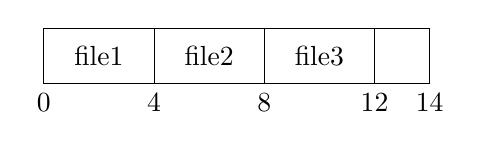
\begin{tikzpicture}[scale=.035]
\draw (0,0) rectangle (40,20);
\draw (40,0) rectangle (80,20);
\draw (80,0) rectangle (120,20);
\draw (120,0) rectangle (140,20);
\draw (20,10) node{file1};
\draw (60,10) node{file2};
\draw (100,10) node{file3};
\draw (0,-7) node{0};
\draw (40,-7) node{4};
\draw (80,-7) node{8};
\draw (120,-7) node{12};
\draw (140,-7) node{14};
\end{tikzpicture}\]
\iffalse
\[\begin{graph}(150,32)(-3,-12)
\graphlinecolour{0}
\fillednodesfalse
\rectnode{a}[40,20](20,10)
\rectnode{b}[40,20](60,10)
\rectnode{c}[40,20](100,10)
\rectnode{d}[20,20](130,10)
\autonodetext{a}{file1}
\autonodetext{b}{file2}
\autonodetext{c}{file3}
\freetext(0,-7){0}
\freetext(40,-7){4}
\freetext(80,-7){8}
\freetext(120,-7){12}
\freetext(140,-7){14}
\end{graph}\]
\fi
Suppose file2 is now deleted, resulting in a four-block gap, with
another two blocks free at the end of the disk:
\[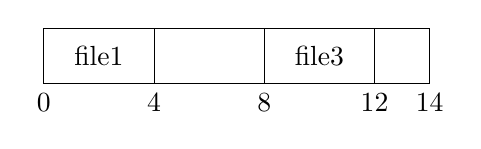
\begin{tikzpicture}[scale=.035]
\draw (0,0) rectangle (40,20);
\draw (40,0) rectangle (80,20);
\draw (80,0) rectangle (120,20);
\draw (120,0) rectangle (140,20);
\draw (20,10) node{file1};
\draw (100,10) node{file3};
\draw (0,-7) node{0};
\draw (40,-7) node{4};
\draw (80,-7) node{8};
\draw (120,-7) node{12};
\draw (140,-7) node{14};
\end{tikzpicture}\]
\iffalse
\[\begin{graph}(150,32)(-3,-12)
\graphlinecolour{0}
\fillednodesfalse
\rectnode{a}[40,20](20,10)
\rectnode{b}[40,20](60,10)
\rectnode{c}[40,20](100,10)
\rectnode{d}[20,20](130,10)
\autonodetext{a}{file1}
\autonodetext{c}{file3}
\freetext(0,-7){0}
\freetext(40,-7){4}
\freetext(80,-7){8}
\freetext(120,-7){12}
\freetext(140,-7){14}
\end{graph}\]
\fi
If, at this point, a three-block file (file4) is created, it can go
into the four-block gap, leaving one block unused:
\[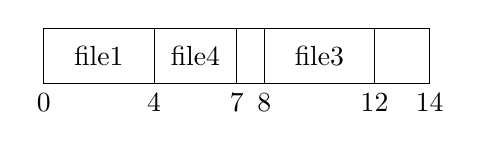
\begin{tikzpicture}[scale=.035]
\draw (0,0) rectangle (40,20);
\draw (40,0) rectangle (70,20);
\draw (70,0) rectangle (80,20);
\draw (80,0) rectangle (120,20);
\draw (120,0) rectangle (140,20);
\draw (20,10) node{file1};
\draw (100,10) node{file3};
\draw (55,10) node{file4};
\draw (0,-7) node{0};
\draw (40,-7) node{4};
\draw (70,-7) node{7};
\draw (80,-7) node{8};
\draw (120,-7) node{12};
\draw (140,-7) node{14};
\end{tikzpicture}\]
\iffalse
\[\begin{graph}(150,32)(-3,-12)
\graphlinecolour{0}
\fillednodesfalse
\rectnode{a}[40,20](20,10)
\rectnode{b}[30,20](55,10)
\rectnode{e}[10,20](75,10)
\rectnode{c}[40,20](100,10)
\rectnode{d}[20,20](130,10)
\autonodetext{a}{file1}
\autonodetext{c}{file3}
\autonodetext{b}{file4}
\freetext(0,-7){0}
\freetext(40,-7){4}
\freetext(70,-7){7}
\freetext(80,-7){8}
\freetext(120,-7){12}
\freetext(140,-7){14}
\end{graph}\]
\fi
Now there are three unused blocks, but there is no way to
satisfy another three-block allocation request, because the three
unused blocks are broken up, with one block between files 4 and 3, and
two more blocks at the end of the disk.

Notice that you wound up with a one-block gap not because a one-block
file was created and later deleted (or because of stupid allocation),
but because a four-block file was replaced by a three-block file.  The
resulting gap is the difference in the file sizes.  This means that
even if a disk is used exclusively for storing large files, it may
still wind up with small gaps, which cannot hold any large files.
This is the fundamental problem of external fragmentation.

Returning to the parallel parking analogy, consider an area where no
parking spaces are marked on the pavement, leaving drivers to allocate
their own spaces.  Even if they are courteous enough not to leave any
pointless gaps, small gaps will arise as cars of varying sizes come
and go.  A large car may vacate a space, which is then taken by a
smaller car.  The result is a gap equal to the difference in car
sizes, too small for even the smallest cars to use.  If this situation
happens repeatedly at different spots along a block, there may be enough
total wasted space to accommodate a car, but not all in one place.

Earlier, I mentioned that increasing the file system block size,
which increases internal fragmentation, decreases external
fragmentation.  The reason for this is that with a larger block size,
there is less variability in the amount of space being allocated.
Files that might have different sizes when rounded up to the next
kilobyte (say, 14~KB and 15~KB) may have the same size when rounded to
the next multiple of 4~KB (in this case, 16~KB and 16~KB).  Reduced
variability reduces external fragmentation; in the extreme case, no
external fragmentation at all occurs if the files are all allocated
the same amount of space.

Suppose you relax the requirement that a file be allocated a single
extent of the disk.  Using file metadata, it is possible to
store different blocks of the file in different locations, much as a
virtual memory address space can be scattered throughout physical
memory.  Does this mean that external fragmentation is a nonissue?
No, because for performance reasons, you will still want to allocate
the file contiguously as much as possible.  Therefore, external
fragmentation will simply change from being a space-efficiency issue
(free space that cannot be used) to a time-efficiency issue (free
space that cannot be used without file access becoming slower).  This
gets us into the next topic, locality.

\subsection{Locality}\label{locality-section}

Recall that disks provide their fastest performance when asked to
access a large number of consecutive sectors in a single request at a
location nearby to the previous access request. Most file system
designers have interpreted these conditions for fast access as implying the following
locality guidelines for space allocation:
\begin{enumerate}
\item The space allocated for each file should be broken into as few
extents as possible.
\item If a file needs to be allocated more than one extent, each
extent should be nearby to the previous one.
\item Files that are commonly used in close succession (or
concurrently) should be placed near one another.
\end{enumerate}

The connection between fast access and these three guidelines is
based on an implicit assumption that the computer system's
workload largely consists of accessing one file at a time and reading
or writing each file in its entirety, from beginning to end.  In some
cases, this is a reasonable approximation to the truth, and so the
preceding locality guidelines do result in good performance.
However, it is important to remember that the guidelines incorporate
an assumption about the workload as well as the disk performance
characteristics.  For some workloads, a different allocation strategy
may be appropriate.  In particular, as computing workloads are
consolidated onto a smaller number of computers
(using techniques such as virtualization, as discussed in Section~\ref{virtual-machines-subsection}),
file accesses become more jumbled.

As an example of a different allocation strategy that might make
sense, Rosenblum and Ousterhout suggested that blocks should be
allocated space on disk in the order they are written, without regard
to what files they belong to or what positions they occupy within
those files.  By issuing a large number of consecutive writes to the
disk in a single operation, this allows top performance for writing.
Even if the application software is concurrently writing to multiple files, and
doing so at random positions within those files, the write operations
issued to disk will be optimal, unlike with the more conventional file
layout.  Of course, read accesses will be efficient only if they are
performed in the same order as the writes were.  Fortunately, some
workloads do perform reads in the same order as writes, and some other
workloads do not need efficient read access.  In particular, the
efficiency of read access is not critical in a workload that reads most disk blocks
either never or repeatedly.  Those blocks that are never read are not a
problem, and those that are read repeatedly need only suffer the cost
of disk access time once and can thereafter be kept in RAM.

Returning to the more mainstream strategy listed at the beginning of
this subsection, the primary open question is how to identify files
that are likely to be accessed contemporaneously, so as to place them
nearby to one another on disk.  One approach, used in UNIX file
systems, is to assume that files are commonly accessed in conjunction
with their parent directory or with other (sibling) files in the same
directory.  Another approach is to not base the file placement on
assumptions, but rather on observed behavior.  (One assumption
remains: that future behavior will be like past behavior.)  For
example, Microsoft introduced a feature into Windows with the XP
version, in which the system observes the order of file accesses at
system boot time and also at application startup time, and then
reorganizes the disk space allocation based on those observed access
orders.  Mac OS~X does something similar as of version 10.3: it
measures which files are heavily used and groups them together.

\subsection{Allocation Policies and Mechanisms}
\label{fs-allocation}

Having seen the considerations influencing disk space allocation
(fragmentation and locality), you are now in a better position to
appreciate the specific allocation mechanism used by any particular
file system and the policy choices embodied in that mechanism.  The
full range of alternatives found in different file systems is too
broad to consider in any detail here, but I will sketch some
representative options.

Each file system has some way of keeping track of which disk blocks
are in use and which are free to be allocated.  The most common
representation for this information is a \vocab{bitmap}, that is, an
array of bits, one per disk block, with bit $i$
indicating whether block $i$ is in use.  With a bitmap, it is easy to
look for space in one particular region of the disk, but slow to
search an entire large disk for a desired size extent of free space.

Many UNIX and Linux file systems use a slight variant on the bitmap
approach.  Linux's ext3fs file system can serve as an example.  The
overall disk space is divided into modest-sized chunks known as
\vocabs{block group}.  On a system with 4-KB disk blocks,
a block group might encompass 128~MB.  Each block group has its own
bitmap, indicating which blocks within that group are free.  (In
Exercise~\ref{block-group-bitmap-exercise}, you can show that in the example given, each block group's
bitmap fits within a single block.)  Summary information for the file
system as a whole indicates how much free space each block group has,
but not the specific location of the free space within the block
groups.  Thus, allocation can be done in two steps: first find a
suitable block group using the summary information, and then find a
suitable collection of blocks within the block group, using its
bitmap.

I remarked earlier that UNIX and Linux file systems generally try to
allocate each file near its parent directory.  In particular, regular
files are placed in the same block group as the parent directory,
provided that there is any space in that group.  If this rule were
also followed for subdirectories, the result would be an attempt to
cram the entire file system into one block group.  Therefore, these
file systems use an alternative rule to choose a block group for a
subdirectory.

When creating a subdirectory, early versions of ext3fs and similar
file systems selected a
block group containing a lot of free space.
This spread the directories, with their corresponding files,
relatively evenly through the whole disk.  Because each new directory
went into a block group with lots of free space, there was a good
chance that the files contained in that directory would fit in the
same block group with it.  However, traversing a directory tree could
take a long time with these allocation policies, because each
directory might be nowhere near its parent directory.

Therefore, more recent versions of ext3fs and similar file systems
have used a different allocation policy for directories, developed by
Orlov.  A subdirectory is allocated in the parent directory's block
group, provided that it doesn't get too crowded.  Failing that, the
allocation policy looks through the subsequent block groups for one
that isn't too crowded.  This preserves locality across entire
directory trees without stuffing any block group so full of
directories that the corresponding files won't fit. The result can be
significant performance improvements for workloads that traverse
directory trees.

Once a file system decides to locate a file within a particular block
group, it still needs to allocate one or more extents of disk blocks
to hold the file's data.  (Hopefully those extents will all lie within
the chosen block group, although there needs to be a way for large
files to escape from the confines of a single block group.)

The biggest challenge in allocating extents is knowing how big an
extent to allocate.  Some older file systems required application
programmers to specify each file's size at the time the file was
created, so that the system could allocate an extent of corresponding
size.  However, modern systems don't work this way; instead, each file
grows automatically to accommodate the data written into it.

To meet this challenge, modern operating systems use a technique known
as \foldvocab{delayed}{allocation}.  As background, you need to
understand that operating systems do not normally write data to disk
the moment an application program issues a write request.  Instead,
the data is stored in RAM and written back to disk later.  This delay
in writing yields two options for when the disk space is allocated:
when the data goes into RAM or later when it gets written to disk.

Without delayed allocation, the operating system needs to choose a
disk block to hold the data at the time it goes into RAM.  The system
tags the data in RAM with the disk block in which that data belongs.  Later,
the system writes the data out to the specified location on disk.
This approach is simple, but requires the operating system to allocate
space for the first block of data as soon as it is generated, before
there is any clue how many more blocks will follow.

Delayed allocation puts off the choice of disk block until the time of
actually writing to disk; the data stored in RAM is tagged only with
the file it should be written to and the position within that file.
Now the operating system does not need to guess how much data a
program is going to write at the time when it generates the first
block.  Instead, it can wait and see how much data gets written and
allocate an extent that size.

Once the operating system knows the desired extent size, it needs to
search the data structure that records the available space.  Bitmaps
(whether in individual block groups or otherwise) are not the only
option for tracking free space.  The XFS file system, which was
particularly designed for large file systems, takes an alternative
approach.  It uses balanced search trees, known as
B-trees, to track the free extents of disk space.  One B-tree
stores the free extents indexed by their location while another
indexes them by their size.  That way, XFS can quickly locate free
space near a specified location on disk or can quickly locate a
desired amount of space.  Technically, the trees used by XFS are a
slight variant of B-trees, known as
B${}^+$-trees.  I'll describe this data
structure in Section~\ref{B-trees}.

With free extents indexed by size in a B${}^+$-tree, the XFS allocator can
naturally use a \vocab{best-fit} policy, where it finds the smallest
free extent bigger than the desired size.  (If the fit is not exact,
the extra space can be broken off and left as a smaller free extent.)
With a bitmap, on the other hand, the most natural allocation policy
is \vocab{first-fit}, the policy of finding the first free extent that is
large enough.  Each policy has its merits; you can compare them in
Exercise~\ref{best-fit-first-fit-exercise}.

\section{Metadata}\label{metadata-section}

You have seen that a file system is analogous to a virtual memory
system.  Each has an allocation policy to select concrete storage
locations for each chunk of data.  Continuing the analogy, I will now
explain the \vocab{metadata} that serves as the analog of page tables.  Recall that in a system with
separate address spaces, each process has its own page table, storing
the information regarding which page frame holds that process's page~0,
page~1, and so forth.  Similarly, each file has its
own metadata storing the information regarding which disk block holds
that file's block~0, block~1, and so forth.  You will see that, as with page
tables, there are several choices for the data structure holding this
mapping information.  I discuss these alternative structures in
Section~\ref{data-location-metadata-section}.

Metadata is data about data.  Information regarding where on disk the
data is stored is one very important kind of metadata.  However, I
will also more briefly enumerate other kinds.
First, in Section~\ref{access-control-metadata-section}, I will
revisit access control, a topic I considered
from another perspective in Chapter~\ref{processes-chapter}.  In Section~\ref{access-control-metadata-section}, the question
is not how access control information is enforced during access
attempts, but how it is stored in the file system.  Second, I will
look in Section~\ref{other-metadata-section} at the other more minor, miscellaneous kinds of metadata (beyond
data location and access control), such as access dates and times.

Some authors include file names as a kind of metadata.  This makes
sense in those file systems where each file has exactly one name.
However, most modern file systems do not fit this description; a file
might have no names, or might have multiple names.  Thus, you are
better off thinking of a name not as a property of a file, but as a
route that can lead to a file.  Similarly, in other persistence
services, data may be accessed through multiple routes, such as
database indexes.  Therefore, I will not include naming in this
section on metadata, instead including it in Section~\ref{directory-indexing-section} on
directories and indexing.

\subsection{Data Location Metadata}\label{data-location-metadata-section}

The simplest representation for data location metadata would be an
array of disk block numbers, with element $i$ of the array specifying
which disk block holds block $i$ of the file.  This would be analogous
to a linear page table.  Traditional UNIX file systems (including
Linux's ext2fs and ext3fs) use this approach for small files.  Each file's
array of disk block numbers is stored in the file's metadata structure
known as its \vocab{inode} (short for
\foldvocab{index}{node}).  For larger files, these file systems keep
the inodes compact by using indirect blocks, roughly
analogous to multilevel page tables.  I discuss the traditional form
of inodes and indirect blocks next.  Thereafter, I discuss two
alternatives used in some more modern file systems: extent maps, which
avoid storing information about individual blocks, and B${}^+$-trees, which
provide efficient access to large extent maps.

\subsubsection{Inodes and Indirect Blocks}

When UNIX was first developed in the early 1970s, one of its many
innovative features was the file system design, a design that has served as the
model for commonly used UNIX and Linux file systems to the present
day, including Linux's ext3fs.  The data-location metadata in these
systems is stored in a data structure that can better be called
expedient than elegant.  However, the structure is efficient for small files,
allows files to grow large, and can be manipulated by simple code.

Each file is represented by a compact chunk of data called an inode.
The inode contains the file's metadata if the file is small or an
initial portion of the metadata if the file is large.  By allowing
large files to have more metadata elsewhere (in indirect blocks), the
inodes are kept to a small fixed size.  Each file system contains an
array of inodes, stored in disk blocks set aside for the purpose,
with multiple inodes per block.  Each inode is identified by its position
in the array.  These inode numbers (or \vocabs{inumber}) are the
fundamental identifiers of the files in a file system; essentially, the
files are identified as
file~0, file~1, and so forth, which indicate the files with inodes in position 0,
1, and so forth.  Later, in Section~\ref{directory-indexing-section}, you'll see
how file names are mapped into inode numbers.

Each inode provides the metadata for one file.  The metadata includes the disk block numbers
holding that file's data, as well as the access permissions and other
metadata.  These categories of metadata are shown in Figure~\ref{initial-inode}.
\begin{figure}
\centerline{\begin{tabular}{|c|}
\hline
file block 0's disk block number\\\hline
file block 1's disk block number\\\hline
file block 2's disk block number\\\hline
$\vdots$\\\hline
access permissions\\\hline
other metadata\\\hline
\end{tabular}}
\caption{This initial approximation of an inode shows the principle
categories of metadata.   However, this diagram is unrealistic in that the list
of disk block numbers seems to be unlimited, whereas actual inodes
have only a limited amount of space.}
\label{initial-inode}
\end{figure}
In this simplified diagram, the inode directly contains the mapping
information specifying which disk block contains each block of the
file, much like a linear page table.  Recall, however, that inodes are
a small, fixed size, whereas files can grow to be many blocks long.
To resolve this conflict, each inode directly contains the mapping
information only for the first dozen or so blocks.  (The exact number
varies between file systems, but is consistent within any one file
system.)  Thus, a more realistic inode picture is as shown in
Figure~\ref{limited-inode}.
\begin{figure}
\centerline{\begin{tabular}{|c|}
\hline
file block 0's disk block number\\\hline
$\vdots$\\\hline
file block 11's disk block number\\\hline
indirect access to file block 12 through the end of the file\\\hline
access permissions\\\hline
other metadata\\\hline
\end{tabular}}
\caption{In this limited-size inode, blocks from number~12 to the end of the
file are indirectly referenced.}
\label{limited-inode}
\end{figure}

Before I go into detail on how further disk blocks are indirectly
accessed, I should emphasize one aspect of the inode design.  The
low-numbered blocks of a file are mapped in the exact same way
(directly in the inode) regardless of whether they are the only blocks
in a small file or the first blocks of a large file.  This means that
large files have a peculiar asymmetry, with some blocks more
efficiently accessible than others.  The advantage is that when a file
grows and transitions from being a small file to being a large one, the
early blocks' mapping information remains unchanged.

Because most files are small, the inodes are kept small, a fraction of
a block in size.  (If inodes were full blocks, the overhead for
single-block files would be 100 percent.)  For those files large enough to
overflow an inode, however, one can be less stingy in allocating space
for metadata.  Therefore, if the system needs more metadata space, it doesn't
allocate a second inode; it allocates a whole additional disk block, an
\foldvocab{indirect}{block}.  This provides room for many more
block numbers, as shown in Figure~\ref{single-indirect-inode}.  The
exact number of additional block numbers depends on how big blocks and
block numbers are.  With 4-KB blocks and 4-byte block numbers, an
indirect block could hold 1~K block numbers (that is, 1024 block
numbers), as shown in the figure.  This kind of indirect block is more
specifically called a \foldvocab{single}{indirect block}, because it
adds only a single layer of indirection: the inode points to it, and
it points to data blocks.
\begin{figure}
\centerline{\begin{tabular}{|c|c|c|}
\multicolumn{1}{c}{\textbf{Inode}}&\multicolumn{1}{c}{\hspace{1em}}&\multicolumn{1}{c}{\textbf{Indirect block}}\\\cline{1-1}\cline{3-3}
file block 0's disk block number&&file block 12's disk block number\\\cline{1-1}\cline{3-3}
$\vdots$&&$\vdots$\\\cline{1-1}\cline{3-3}
file block 11's disk block number&&file block 1035's disk block number\\\cline{1-1}\cline{3-3}
indirect block's block number&\multicolumn{1}{c}{}&\multicolumn{1}{c}{}\\\cline{1-1}
access permissions&\multicolumn{1}{c}{}&\multicolumn{1}{c}{}\\\cline{1-1}
other metadata&\multicolumn{1}{c}{}&\multicolumn{1}{c}{}\\\cline{1-1}
\end{tabular}}
\caption{If an inode were used with a single indirect block, the block
numbers would be stored as shown here. Note that the indirect
block is actually considerably larger than the inode, contrary to its
appearance in the figure.}
\label{single-indirect-inode}
\end{figure}

In this example with 4-KB blocks, the single indirect block allows you
to accommodate files slightly more than 4~MB in size.  To handle
yet-larger files, you can use a multilevel tree scheme, analogous to
multilevel page tables.  The inode can contain a block number for a
double indirect block, which contains block numbers for many more
single indirect blocks, each of which contains many data block
numbers.  Figure~\ref{double-indirect-inode} shows this enhancement to
the inode design, which retains the dozen direct blocks and the original single
indirect block, while adding a double indirect block.
\begin{figure}
\centerline{\begin{tabular}{|c|c|c|}
\multicolumn{1}{c}{\textbf{Inode}}&\multicolumn{1}{c}{\hspace{1em}}&\multicolumn{1}{c}{\textbf{Single
indirect block}}\\\cline{1-1}\cline{3-3}
file block 0's disk block number&&file block 12's disk block number\\\cline{1-1}\cline{3-3}
$\vdots$&&$\vdots$\\\cline{1-1}\cline{3-3}
file block 11's disk block number&&file block 1035's disk block number\\\cline{1-1}\cline{3-3}
single indirect block's number&\multicolumn{1}{c}{}&\multicolumn{1}{c}{}\\\cline{1-1}
double indirect block's number&\multicolumn{1}{c}{}&\multicolumn{1}{c}{}\\\cline{1-1}
access permissions&\multicolumn{1}{c}{}&\multicolumn{1}{c}{}\\\cline{1-1}
other metadata&\multicolumn{1}{c}{}&\multicolumn{1}{c}{}\\\cline{1-1}
\end{tabular}}
\vspace*{1em}
\centerline{\begin{tabular}{|c|c|c|}
\multicolumn{1}{c}{\textbf{Double indirect
block}}&\multicolumn{1}{c}{\hspace{1em}}&\multicolumn{1}{c}{\textbf{Indirect
block 1}}\\\cline{1-1}\cline{3-3}
indirect block 1's block number&&file block 1036's disk block number\\\cline{1-1}\cline{3-3}
$\vdots$&&$\vdots$\\\cline{1-1}\cline{3-3}
indirect block 1024's block number&&file block 2059's disk block number\\\cline{1-1}\cline{3-3}
\end{tabular}}
\vspace*{1em}
\textbf{Indirect blocks 2--1024:} similar to indirect block 1
\caption{If an inode were used with single and double indirect blocks,
the block numbers would be stored as shown here.}
\label{double-indirect-inode}
\end{figure}

Because the double indirect block points at many indirect blocks, each
of which points at many data blocks, files can now grow quite large.
(In Exercise~\ref{largest-double-indirect-exercise}, you can figure out just how large.)  However, many
UNIX file systems go one step further by allowing the inode to point
to a triple indirect block as well, as shown in
Figure~\ref{inode-block-tree}.  Comparing this with multilevel page
tables is illuminating; the very unbalanced tree used here allows a
small, shallow tree to grow into a large, deeper tree in a
straightforward way.  Later you'll see that B${}^+$-trees grow somewhat less
straightforwardly, but without becoming so imbalanced.
\begin{figure}
\centerline{\includegraphics{hail_f0810}}
\iffalse
\centerline{\begin{graph}(417,140)(8,355)
\graphnodesize{0}
\graphnodecolour{1}
\grapharrowlength{5}
\textnode{inode}(200, 490){inode}[\graphlinewidth{0}\graphlinecolour{1}]
\textnode{directl}(20, 465){}[\graphlinewidth{0}\graphlinecolour{1}]
\freetext(91,472){\ldots}
\textnode{directr}(80, 465){}[\graphlinewidth{0}\graphlinecolour{1}]
\textnode{direct}(50, 460){a few data blocks}[\graphlinewidth{0}\graphlinecolour{1}]
\textnode{single}(142, 460){single indirect}[\graphlinewidth{0}\graphlinecolour{1}]
\textnode{double}(244, 460){double indirect}[\graphlinewidth{0}\graphlinecolour{1}]
\textnode{triple}(346, 460){triple indirect}[\graphlinewidth{0}\graphlinecolour{1}]
\textnode{sdatal}(112, 435){}[\graphlinewidth{0}\graphlinecolour{1}]
\freetext(142,445){\ldots}
\textnode{sdatar}(172, 435){}[\graphlinewidth{0}\graphlinecolour{1}]
\textnode{sdata}(142, 430){many data blocks}[\graphlinewidth{0}\graphlinecolour{1}]
\textnode{dsinglel}(214, 435){}[\graphlinewidth{0}\graphlinecolour{1}]
\freetext(244,445){\ldots}
\textnode{dsingler}(274, 435){}[\graphlinewidth{0}\graphlinecolour{1}]
\textnode{dsingle}(244, 430){many indirect blocks}[\graphlinewidth{0}\graphlinecolour{1}]
\textnode{dsinglelb}(214, 425){}[\graphlinewidth{0}\graphlinecolour{1}]
\textnode{dsinglerb}(274, 425){}[\graphlinewidth{0}\graphlinecolour{1}]
\textnode{dsdatall}(204, 405){}[\graphlinewidth{0}\graphlinecolour{1}]
\freetext(217,413){\ldots}
\textnode{dsdatalr}(234, 405){}[\graphlinewidth{0}\graphlinecolour{1}]
\freetext(244,417){\ldots}
\textnode{dsdatarl}(254, 405){}[\graphlinewidth{0}\graphlinecolour{1}]
\freetext(271,413){\ldots}
\textnode{dsdatarr}(284, 405){}[\graphlinewidth{0}\graphlinecolour{1}]
\textnode{dsdata}(244, 400){tons of data blocks}[\graphlinewidth{0}\graphlinecolour{1}]
\textnode{tdoublel}(316, 435){}[\graphlinewidth{0}\graphlinecolour{1}]
\freetext(346,445){\ldots}
\textnode{tdoubler}(376, 435){}[\graphlinewidth{0}\graphlinecolour{1}]
\textnode{tdouble}(346, 430){many double}[\graphlinewidth{0}\graphlinecolour{1}]
\textnode{tdoubleb}(346, 420){indirect blocks}[\graphlinewidth{0}\graphlinecolour{1}]
\textnode{tdoublelb}(316, 415){}[\graphlinewidth{0}\graphlinecolour{1}]
\textnode{tdoublerb}(376, 415){}[\graphlinewidth{0}\graphlinecolour{1}]
\textnode{tdsinglell}(306, 395){}[\graphlinewidth{0}\graphlinecolour{1}]
\freetext(319,403){\ldots}
\textnode{tdsinglelr}(336, 395){}[\graphlinewidth{0}\graphlinecolour{1}]
\freetext(346,407){\ldots}
\textnode{tdsinglerl}(356, 395){}[\graphlinewidth{0}\graphlinecolour{1}]
\freetext(373,403){\ldots}
\textnode{tdsinglerr}(386, 395){}[\graphlinewidth{0}\graphlinecolour{1}]
\textnode{tdsingle}(346, 390){tons of indirect blocks}[\graphlinewidth{0}\graphlinecolour{1}]
\textnode{tdsinglelb}(316, 385){}[\graphlinewidth{0}\graphlinecolour{1}]
\textnode{tdsinglerb}(376, 385){}[\graphlinewidth{0}\graphlinecolour{1}]
\textnode{tdsdatall}(306, 365){}[\graphlinewidth{0}\graphlinecolour{1}]
\freetext(319,373){\ldots}
\textnode{tdsdatalr}(336, 365){}[\graphlinewidth{0}\graphlinecolour{1}]
\freetext(346,377){\ldots}
\textnode{tdsdatarl}(356, 365){}[\graphlinewidth{0}\graphlinecolour{1}]
\freetext(373,373){\ldots}
\textnode{tdsdatarr}(386, 365){}[\graphlinewidth{0}\graphlinecolour{1}]
\textnode{tdsdata}(346, 360){astronomically many data blocks}[\graphlinewidth{0}\graphlinecolour{1}]
\diredge{inode}{directl}
\diredge{inode}{directr}
\diredge{inode}{single}
\diredge{inode}{double}
\diredge{inode}{triple}
\diredge{single}{sdatal}
\diredge{single}{sdatar}
\diredge{double}{dsinglel}
\diredge{double}{dsingler}
\diredge{dsinglelb}{dsdatall}
\diredge{dsinglelb}{dsdatalr}
\diredge{dsinglerb}{dsdatarl}
\diredge{dsinglerb}{dsdatarr}
\diredge{triple}{tdoublel}
\diredge{triple}{tdoubler}
\diredge{tdoublelb}{tdsinglell}
\diredge{tdoublelb}{tdsinglelr}
\diredge{tdoublerb}{tdsinglerl}
\diredge{tdoublerb}{tdsinglerr}
\diredge{tdsinglelb}{tdsdatall}
\diredge{tdsinglelb}{tdsdatalr}
\diredge{tdsinglerb}{tdsdatarl}
\diredge{tdsinglerb}{tdsdatarr}
\end{graph}}
\fi
\caption{The full structure of a file starts with an inode and
continues through a tree of single, double, and triple indirect
blocks, eventually reaching each of the data blocks.}
\label{inode-block-tree}
\end{figure}

Having presented this method of mapping file blocks into disk blocks, I
will shortly turn to an alternative that avoids storing information on
a per-block basis.  First, however, it is worth drawing one more
analogy with page tables.  Just as a page table need not provide a
page frame number for every page (if some pages are not in memory), an
inode or indirect block need not provide a disk block number for every
block of the file.  Some entries can be left blank, typically by using
some reserved value that cannot be mistaken for a legal disk block
number.  This is valuable for \foldvocabs{sparse}{file}, also known as
files with \vocabs{hole}.  A sparse file has one or more large
portions containing nothing but zeros, usually because those portions
have never been written.  By not allocating disk blocks for the
all-zero file blocks, the file system can avoid wasting space and time.

\subsubsection{Extent Maps}

You have seen that traditional inodes and indirect blocks are based
around the notion of a \foldvocab{block}{map}, that is, an array
specifying a disk block number for each file block.  A block map is
completely general, in that each file block can be mapped to any disk
block.  File block $n$ can be mapped somewhere totally different on
disk from file block $n-1$.  Recall, however, that file system designers prefer
not to make use of this full generality.  For performance reasons,
consecutive file blocks will normally be allocated consecutive disk
blocks, forming long extents.  This provides the key to a more
efficient data structure for storing the mapping information.

Suppose you have a file that is 70 blocks long and that occupies
disk blocks 1000--1039 and 1200--1229.  A
block map would contain each one of those 70 disk block numbers.  An
\foldvocab{extent}{map}, on the other hand, would contain only two
entries, one for each of the file's extents, just as the opening
sentence of this paragraph contains two
ranges of block numbers.  Each entry in the extent
map needs to contain enough information to describe one extent.  There
are two alternatives for how this can be done:
\begin{itemize}
\item
Each entry can contain the extent's length and starting disk block
number.  In the example, the two extent map entries would be $(40,
1000)$ and $(30, 1200)$.  These say the file contains 40 blocks
starting at disk block 1000 and 30 blocks starting at disk block
1200.
\item
Each entry can contain the extent's length, starting file block
number, and starting disk block number.  In the example, the two
extent map entries would be $(40, 0, 1000)$ and $(30, 40, 1200)$.  The
first entry describes an extent of 40 blocks, starting at position 0 in the
file and occupying disk blocks starting with number 1000.  The second entry
describes an extent of 30 blocks, starting
at position 40 in the file and occupying disk blocks starting with number 1200.
\end{itemize}
The first approach is more compact.  The second approach, however, has the
advantage that each extent map entry can be understood in isolation,
without needing to read the preceding extent map entries.  This is
particularly useful if the extent map is stored in a B${}^+$-tree, as I
will discuss subsequently. For simplicity, I will assume the second approach
in the remainder of my discussion, though there are systems that use
each.

At first, it may not be obvious why extent maps are a big improvement.
A typical block map system might use a 4-byte block number to refer
to each 4-KB block.  This is less than one-tenth of one percent space
overhead, surely affordable with today's cheap disk storage.  What
reason do file system designers have to try to further reduce such an already small
overhead?  (I will ignore the possibility that the extent map takes
more space than the block map, which would happen only if the file is
scattered into lots of tiny extents.)

The key fact is that disk space efficiency turns into time efficiency,
which is a much more precious commodity.  Indirect blocks result in
extra disk I/O operations.  Consider, for example, reading a file that
is stored in a single 20-block extent.  With the block map
approach, the file system would need to do at least two disk read
operations: one to read the single indirect block and one to read the
data blocks.  This assumes the inode is already cached in memory,
having been read in along with other inodes in its disk block, and
that the file system is smart enough to read all 20 data blocks in
a single operation.  With an extent map, the entire mapping
information would fit in the inode; if you again assume the inode is
cached, a single read operation suffices.  Thus, the system can read
files like this twice as fast.  Admittedly, this is a somewhat
artificial best-case example.  However, even with realistic workloads,
a significant speedup is possible.

Several modern file systems use extent maps, including Microsoft
Windows' NTFS, Mac OS~X's HFS Plus, and XFS, which was ported into
Linux from SGI's IRIX version of UNIX.  For files that have only a
handful of extents (by far the most common case), all three store the
sequence of extent map entries in the inode or (in Windows and Mac
OS~X) in the corresponding inode-like structure.  The analogs of inodes in
NTFS are large enough (1~KB) that they can directly store entire
extent maps for most files, even those with more than a few extents. The other
two file systems use smaller inodes (or inode-like structures) and so
provide an interesting comparison of techniques for handling the
situation where extra space is needed for a large extent map.

HFS Plus takes an approach quite reminiscent of traditional UNIX
inodes: the first eight extent map entries are stored directly in the
inode-like structure, whether they are the only ones or just the first
few of a larger number.  Any additional entries are stored elsewhere,
in a single B${}^+$-tree that serves for all the files, as I will describe
subsequently.  XFS, on the other hand, stores all the extent map entries for
a file in a file-specific B${}^+$-tree; the space in the inode is the root
node of that tree.  When the tree contains only a few extents, the
tree is small enough that the
root of the tree is also a leaf, and so the extents are directly in
the inode, just as with HFS Plus.  When the extent map grows larger,
however, all the entries move down into descendant nodes in the tree,
and none are left in the inode, unlike HFS Plus's special treatment of
the first eight.

\subsubsection{B-Trees}\label{B-trees}

The \vocab{B-tree} data structure is a balanced search tree structure
generally configured with large, high-degree nodes forming shallow,
bushy trees.  This property makes it well suited to disk storage,
where transferring a large block of data at once is efficient (hence,
large nodes), but performing a succession of operations is slow (hence,
a shallow tree).  You may have encountered B-trees before,
in which case my summary will be a review, with the exception
of my description of specific applications for which this structure
is used.

Any B-tree associates search keys with corresponding values, much like
a dictionary associates words with their definitions or a phone book
associates names with phone numbers.  The keys can be textual strings
organized in alphabetic order (as in these examples) or numbers
organized by increasing value; all that is required is that there is
some way to determine the relative order of two keys.

The B-tree allows entries to be efficiently located by key, as well as
inserted and deleted.  Thus far, the same could be said for a hash
table structure, such as is used for hashed page tables.  Where
B-trees (and other balanced search trees) distinguish themselves is
that they also provide efficient operations based on the ordering of
keys, rather than just equality of keys.  For example, if someone asks
you to look up ``Smit'' in a phone book, you could reply, ``There is no
Smit; the entries skip right from Smirnoff to Smith.''  You could do
the same with a B-tree, but not with a hash table.

This ability to search for neighbors of a key, which need not itself
be present in the tree, is crucial when B-trees are used for extent
maps.  Someone may want information about the extent containing file
block 17.  There may be no extent map entry explicitly mentioning 17;
instead, there is an entry specifying a 10-block extent starting with
file block 12.  This entry can be found as the one with the largest key
that is less than or equal to 17.

B-trees can play several different roles in persistence systems.  In
Section~\ref{directory-indexing-section}, you'll see their use for
directories of file names and for indexes of database contents; both
are user-visible data access services.  In the current section,
B-trees play a
more behind-the-scenes role, mapping positions within a file to
locations on disk.  Earlier, in Section~\ref{fs-allocation}, you saw
another related use, the management of free space for allocation.  The
data structure fundamentals are the same in all cases; I choose to
introduce them here, because extent maps seem like the simplest
application.  Free space mapping is complicated by the dual indexing
(by size and location), and directories are complicated by the use of
textual strings as keys.

You are probably already familiar with binary search trees, in which
each tree node contains a root key and two pointers to subtrees, one
with keys smaller than the root key, and one with keys larger than the
root key.  (Some convention is adopted for which subtree contains keys
equal to the root key.)  B-tree nodes are similar, but rather than
using a single root key to make a two-way distinction, they use $N$
root keys to make an $N+1$ way distinction.  That is, the root node
contains $N$ keys (in ascending order) and $N+1$ pointers to subtrees,
as shown in Figure~\ref{scan-8-1}.
\begin{figure}
\centerline{\includegraphics{hail_f0811}}
%\centerline{\def\epsfsize#1#2{0.6#1}\epsfbox{scan-8-1.eps}}
\caption{A B-tree node contains $N$ keys and $N+1$ pointers to the
subtrees under it.  Each subtree contains keys in a particular range.}
\label{scan-8-1}
\end{figure}
The first subtree contains keys smaller than the first root key, the
next subtree contains keys between the first and second root keys,
and so forth.  The last subtree contains keys larger than the last root key.

If a multi-kilobyte disk block is used to hold a B-tree node, the
value of $N$ can be quite large, resulting in a broad, shallow tree.
In fact, even if a disk block were only half full with root keys and
subtree pointers, it would still provide a substantial branching
factor.  This observation provides the inspiration for the mechanism
used to maintain B-trees as entries are inserted.

Each node is allowed to be anywhere between half full and totally
full.
This flexibility means one can easily insert into a node, so long as
it is less than full.
The hard case can be handled by
splitting nodes.  As a special exception, the root node is not
required to be even half full.  This exception allows you to build a
tree with any number of entries, and it adds at most one level to the height
of the tree.

Consider, for example, inserting one more entry into an already full
node.  After insertion, you have $N+1$ keys but only room for $N$.  The node
can be replaced with two nodes, one containing the $N/2$ smallest keys
and the other the $N/2$ largest keys.  Thus, you now have two half-full
nodes.  However, you have only accounted for $N$ of the $N+1$ keys; the
median key is still left over.  You can insert this median key into the
parent node, where it will serve as the divider between the two
half-full nodes, as shown in Figure~\ref{B-tree-split}.
\begin{figure}
\centerline{\includegraphics{hail_f0812}}
%\centerline{\def\epsfsize#1#2{0.6#1}\epsfbox{B-tree-split.eps}}
\caption{Inserting 16 into the illustrated B-tree, which has
node-capacity 4, causes a node to split, with the median key moving
into the parent.}
\label{B-tree-split}
\end{figure}

When you insert the median key into the parent node, what if the
parent node is also full?  You split the parent as well.  The splitting
process can continue up the tree, but because the tree is shallow, this
won't take very long.  If the node being split has no parent, because
it is the root of the tree, it gains a new parent holding just the
median key.  In this way the tree grows in height by one level.

In Bayer and McCreight's 1972 paper introducing B-trees, they
suggested that each node contain key/value pairs, along with pointers
to subtrees.  Practical applications today instead use a variant,
sometimes called \vocabindex{B${}^+$-trees}{B-tree}.  In a
B${}^+$-tree, the nonleaf nodes contain just keys and pointers to
subtrees, without the keys having any associated values.  The keys in
these nodes are used solely for navigation to a subtree.  The leaves
contain the key/value pairs that are the actual contents of the data
structure.  For example, a small B${}^+$-tree of extent map entries
might be organized as shown in Figure~\ref{B-plus-tree}.
\begin{figure}
\centerline{\includegraphics{hail_f0813}}
%\centerline{\def\epsfsize#1#2{0.6#1}\epsfbox{B-plus-tree.eps}}
\caption{This small B${}^+$-tree extent map contains information that
can be used to find
each extent's range of file block numbers and range of disk block
numbers.  Because the tree is a B${}^+$-tree rather than a B-tree, all
the extents are described in the leaves, with the nonleaf node containing
just navigational information.}
\label{B-plus-tree}
\end{figure}

This sort of B${}^+$-tree can store the extent map for a single file,
as is done in XFS.  For Mac OS~X's HFS Plus, a slightly different
approach is needed, because all files' extent maps are combined into a
single B${}^+$-tree.  (Recall, though, that the first eight extents of
each file are not included in this tree.)

Each entry in this file system's B${}^+$-tree describes an extent map
entry for some position within some file.  That is, the entry contains
a file number (analogous to an inode number), a starting block number
within the file, a length in blocks, and a starting disk block
number.  The concatenation of file number and starting file block
number serves as the key.  That way, all the entries for a particular
file appear consecutively in the tree, in order by their position
within the file.

The insertion algorithm for B${}^+$-trees is a slight variant of the
one for pure B-trees; you can work through the differences in
Exercise~\ref{Bplus-tree-insertion-exercise}.

\subsection{Access Control Metadata}\label{access-control-metadata-section}

The complexity of the data structures storing access control
information is directly related to the sophistication of the
protection system.  Recall that the POSIX specification, followed by
UNIX and Linux, provides for only fixed-length access control lists
(ACLs), with permissions for a file's owner, owning group, and
others.  This information can be stored compactly in the file's
inode.  Microsoft Windows, on the other hand, allows much more general
ACLs.  Thus, the designers of NTFS have faced a more interesting
challenge and, in fact, have revisited their design decision, as you
will see.

For POSIX-compliant access control, an inode can contain three
numbers: one identifying the file's owning user, one identifying the
file's owning group, and one containing nine bits, representing the
\verb|rwx| permissions for the owning user, the owning group, and other users.  This third
number, containing the nine permission bits, is called the file's
\vocab{mode}.  Rather than waste all but nine bits in the mode, the
others are used to encode additional information, such as whether the
file is a regular file, a directory, an I/O device, and so forth.
Figure~\ref{stater-source} shows how the permissions can be determined
by extracting an inode's mode using the {\tt stat} system call.  (This
system call differs only slightly from {\tt fstat}, which you saw
earlier.  The file is specified by name, rather than by a numerical
file descriptor.)  If you compile this C$++$ program and call the
resulting executable {\tt stater}, then a command like
\verb|./stater somefile| should produce information you could also get
with \verb|ls -l somefile|.
\begin{figure}
\begin{verbatim}
#include <unistd.h>
#include <time.h>
#include <sys/stat.h>
#include <stdio.h>
#include <iostream>
using namespace std;

static void print_bit(int test, char toPrint){
  if(test)
    cout << toPrint;
  else
    cout << '-';
}

int main(int argc, char *argv[]){
  if(argc != 2){
    cerr << "Usage: " << argv[0] << " filename" << endl;
    return -1;
  }
  struct stat info;
  if(stat(argv[1], &info) < 0){
    perror(argv[1]);
    return -1;
  }
  print_bit(info.st_mode & S_IRUSR, 'r');
  print_bit(info.st_mode & S_IWUSR, 'w');
  print_bit(info.st_mode & S_IXUSR, 'x');
  print_bit(info.st_mode & S_IRGRP, 'r');
  print_bit(info.st_mode & S_IWGRP, 'w');
  print_bit(info.st_mode & S_IXGRP, 'x');
  print_bit(info.st_mode & S_IROTH, 'r');
  print_bit(info.st_mode & S_IWOTH, 'w');
  print_bit(info.st_mode & S_IXOTH, 'x');
  cout << endl;
  return 0;
}
\end{verbatim}
\caption{This C$++$ program, {\tt stater.cpp}, uses {\tt stat} to
  retrieve access control metadata for whichever file is specified by
  the command-line argument {\tt argv[1]}.}
\label{stater-source}
\end{figure}

Early versions of NTFS stored the full ACL for each file
independently.  If the ACL was small enough to fit in the inode-like
structure, it was stored there.  Otherwise, it was stored in one or
more extents of disk blocks, just like the file's data, and the
inode-like structure contained an extent map for the ACL.

As of Windows 2000, Microsoft redesigned NTFS to take advantage of the
fact that many files have identical ACLs.  The contents of the ACLs are
now stored in a centralized database.  If two files have identical
ACLs, they can share the same underlying representation of that ACL.

\subsection{Other Metadata}\label{other-metadata-section}

Because files can be of any length, not just a multiple of the block
size, each inode (or equivalent) contains the file's size in bytes.
(The program in Figure~\ref{fstater-source} on page~\pageref{fstater-source} showed how you can
retrieve this information.)  Other metadata is much more
system-specific.  For example, POSIX specifies that each file has
three time stamps, recording when the file was last accessed, last
written, and last modified in any way. Modification includes not only  writing the
data, but also making changes in
permission and other metadata attributes.  NTFS records whether
the file should be hidden in ordinary directory listings.  HFS Plus
has many metadata attributes supporting the graphical user interface;
for example, each file records its icon's position.

One metadata attribute on POSIX systems connects with file linking,
that is, the use of multiple names for one file, which is the
topic of Section~\ref{file-linking-section}.  Each file's inode contains a count of how many names
refer to the file.  When that count reaches zero and the file is not
in use by any process, the operating system deletes the file.  The
operation users normally think of as deleting a file actually just
removes a name; the underlying file may or may not be deleted as a
consequence.

\section{Directories and Indexing}
\label{directory-indexing-section}

Having seen how file systems provide the storage for files, you are now ready to
consider how those
systems allow files to be located by name.  As a similar question regarding
database systems, you can consider how those systems provide indexed lookup.  In
Section~\ref{directory-index-comparison-section}, I set the stage for
this discussion by presenting a common framework for file directories
and database indexes, showing the ways in which they differ.
In Section~\ref{spotlight-section}, I show how the separation
between file directories and database indexes is currently weakening
with the introduction of indexing mechanisms for locating files.
Having shown the basic principles of both directories and indexes, I use
Section~\ref{file-linking-section} to dig into one particular aspect of
file directories in more detail: the ways in which multiple names can
refer to a single file.  Finally, in
Section~\ref{directory-index-structures-section}, I take you behind
the scenes to look at typical data structures used for directories and indexes.

\subsection{File Directories Versus Database Indexes}\label{directory-index-comparison-section}

Traditionally, file systems include \vocabyies{director}, which provide access
to files by name.  Databases, on the other hand, include \vocabes{index},
which provide access to entries in the database based on a portion of
the contents.  This clean distinction between file systems and
databases is currently blurring, as alternative file-access techniques
based on indexes become available.  In particular, Apple introduced
such a feature in Mac OS~X version 10.4 under the name Spotlight.  I
describe Spotlight in Section~\ref{spotlight-section}.  Microsoft
subsequently included a related feature in
Windows Vista.  This trend makes it even more
important to see what directories and indexes have in common and what
distinguishes them.

Both directories and indexes provide a mapping from keys to objects.
The keys in a directory are names, which are external to the object
being named.  You can change the contents of a file without changing
its name or change the name without changing the contents.  In
contrast, the keys in an index are attributes of the indexed objects,
and so are intrinsic to those objects.  For example, an index on a
database table of chapters might allow direct access to the row with
title {\tt "\persistenceChapterTitle"} or with the number {\tt
\ref{persistence-chapter}}.  If the row were updated to show a change
in this chapter's title or number, the index would need to be updated
accordingly.  Similarly, any update to the index must be in the context of
a corresponding change to
the indexed row; it makes no sense to say that you want
to look up the row under chapter number {\tt 1}, but there find that
the real chapter number is still {\tt \ref{persistence-chapter}}.

Each name in a directory identifies a single file.  Two files may have
the same name in different directories, but not in the same directory.
Database indexes, on the other hand, can be either for a unique
attribute or a non-unique one.  For example, it may be useful to index
a table of user accounts by both the unique login name and the
non-unique last name.  The unique index can be used to find the single
record of information about the user who logs in as {\tt "jdoe"},
whereas the non-unique index can be used to find all the records of
information about users with last name {\tt "Doe"}.    An index can
also use a combination of multiple attributes as its key.  For
example, a university course catalog could have a unique index
keyed on the combination of department and course number.

The final distinction between file directories and database indexes is
the least fundamental; it is the kind of object to which they provide
access.  Traditionally, directories provide access to entire files,
which would be the analog of tables in a relational database.
Indexes, on the other hand, provide access not to entire tables, but
rather to individual rows within those tables.  However, this
distinction is misleading for two reasons:
\begin{itemize}
\item
Database systems typically have a meta-table that serves as a catalog
of all the tables.  Each row in this meta-table describes one table.
Therefore, an index on this meta-table's rows is really an index of
the tables.  Access to its rows is used to provide access to the
database's tables.
\item
As I mentioned earlier, operating system developers are incorporating
indexes in order to provide content-based access to files.  This is
the topic of Section~\ref{spotlight-section}.
\end{itemize}

\subsection{Using Indexes to Locate Files}\label{spotlight-section}

As I have described, files are traditionally accessed by name, using
directories.  However, there has been considerable interest recently
in using indexes to help users locate files by content or other
attributes. Suppose that I could not remember the name
of the file containing this book.  That would not be a disaster, even
leaving aside the possibility that the world might be better off
without the book.  I could search for the file in numerous ways; for
example, it is one of the few files on my computer that has hundreds
of pages.  Because the Mac OS X system that I am using indexes files
by page count (as well as by many other attributes), I can simply ask for all
files with greater than 400 pages.  Once I am shown the five files
meeting this restriction, it is easy to recognize the one I am seeking.

The index-based search feature in Mac OS X, which is called Spotlight,
is not an integral component of the file system in the way directories
and filenames are.  Instead, the indexing and search are provided by
processes external to the operating system, which can be considered a
form of middleware.

The file system supports the indexing through a generic ability to
notify processes of events such as the creation or deletion of a file,
or a change in a file's contents.  These events can be sent to any
process that subscribes to them and are used for other purposes as
well, such as keeping the display of file icons up to date.  The
Spotlight feature uses it to determine when files need reindexing.
When I save out a new version of my book, the file system
notifies Spotlight that the file changed, allowing Spotlight to update
indexes such as the one based on page count.  Unlike file directories,
which are stored in a special data structure internal to the
file system, the indexes for access based on contents or attributes
like page counts are stored in normal files in the
\verb|/.Spotlight-V100| directory.

Apple refers to the indexed attributes (other than the actual file
contents) as metadata.  In my book example, the number of pages in a
document would be one piece of metadata.  This usage of the word
``metadata'' is rather different from its more traditional use in
file systems.  Every file has a fixed collection of file system metadata
attributes, such as owner, permissions, and time of last modification.
By contrast, the Spotlight metadata attributes are far more numerous,
and the list of attributes is open-ended and specific to
individual types of files.  For example, while the file containing my
book has an attribute specifying the page count, the file containing one of my
vacation photos has an attribute specifying the exposure time in
seconds.
Each attribute makes sense for the corresponding
file, but would not make sense for the other one.

As you have seen, the metadata attributes that need indexing are
specific to individual types of files.  Moreover, even common
attributes may need to be determined in different ways for different
types of files.  For example, reading a PDF file to determine its
number of pages is quite different from reading a Microsoft Word file
to determine its number of pages---the files are stored in totally
different formats.  Therefore, when the indexing portion of Spotlight
receives notification from the file system indicating that a file has
changed, and hence should be indexed, it delegates the actual indexing
work to a specialist indexing program that depends on the type of
file.  When you install a new application program on your system, the
installation package can include a matching indexing program.  That
way you will always be able to search for files on your system using
relevant attributes, but without Apple having had to foresee all the
different file types.

\subsection{File Linking}\label{file-linking-section}

Indexed attributes, such as page counts, are generally not unique.  My
system may well have several five-page documents.  By contrast, you have
already seen that each name within a directory names a single file.
Just because each pathname specifies a single file does not mean the
converse is true, however.  In this subsection, I will explain two
different ways in which a file can be reachable through multiple
names.

The most straightforward way in which multiple names can reach a
single file is if the directory entry for each of the names specifies
the same file.  Figure~\ref{hardlink} shows a directory with two
names, both referring to the same file.  In interpreting this figure, you should
understand that the box labeled as the file does not denote just the
data contained in the file, but also all of the file's metadata,
such as its permissions.
\begin{figure}
\centerline{\includegraphics{hail_f0815}}
%\centerline{\def\epsfsize#1#2{0.6#1}\epsfbox{hardlink.eps}}
\caption{A directory can contain two names for one file.}\label{hardlink}
\end{figure}
In the POSIX API, this
situation could have arisen in at least two different ways:
\begin{itemize}
\item
The file was created with the name \verb|alpha|, and then the
procedure call \verb|link("alpha", "beta")| added the name \verb|beta|.
\item
The file was created with the name \verb|beta|, and then the
procedure call \verb|link("beta", "alpha")| added the name \verb|alpha|.
\end{itemize}
No matter which name is the original and which is added, the two play
identical roles afterward, as shown in Figure~\ref{hardlink}.  Neither can be
distinguished as the ``real'' name.  Often people talk of the added
name as a \vocab{link} to the file.  However, you need to understand that \emph{all} file
names are links to files.  There is nothing to distinguish one added
with the \verb|link| procedure.

POSIX allows a file to have names in multiple directories, so long as all the directories are in the same file system.  In the
previous illustration (Figure~\ref{hardlink}),
\verb|alpha| and \verb|beta| in the current directory named one
file. Instead, I could have had directory entries in multiple
directories all pointing at the same file.  For example, in
Figure~\ref{multidirhardlink}, I show a situation where
\verb|/alpha/beta| is a name for the same file as \verb|/gamma/delta|.
\begin{figure}
\centerline{\includegraphics{hail_f0816}}
%\centerline{\def\epsfsize#1#2{0.6#1}\epsfbox{multidirhardlink.eps}}
\caption{A file can have two different names, each in its own
directory.  In this example, the two pathnames {\tt /alpha/beta} and
{\tt /gamma/delta} both lead to the same file.}\label{multidirhardlink}
\end{figure}

To keep the directory structure from getting too tangled, POSIX
systems ordinarily do not allow a directory to have more than one
name.  One exception is that each directory contains two special
entries: one called \verb|.| that is an extra link to that directory
itself and one called \verb|..| that is an extra link to its parent
directory.

Just as \verb|link| adds a name for a file, \verb|unlink| removes a
name.  For example, \verb|unlink("/alpha/beta")| would eliminate one of
the two routes to the file in Figure~\ref{multidirhardlink} by
removing the \verb|beta| entry from the directory \verb|alpha|.  As
mentioned earlier, removing a name only implicitly has anything to do
with removing a file.  The operating system removes the file when it
no longer has any names and is no longer in use by any process.  (An
open file can continue to exist without any names, as you can
demonstrate in Exploration Project~\ref{unlinked-file-project}.)

POSIX also supports another alternative for how multiple names can
lead to one file. One name can refer to another name and
thereby indirectly refer to the same file as the second name.  In this
situation, the first name is called a \foldvocab{symbolic}{link}.
Figure~\ref{symlink} shows an example, where \verb|alpha| is specified
as a symbolic link to \verb|beta|, and thereby refers to
whatever file \verb|beta| does.  (Symbolic links are also sometimes
called \foldvocabs{soft}{link}.  Ordinary links are called
\foldvocabs{hard}{link} when it is important to emphasize the difference.)
\begin{figure}
\centerline{\includegraphics{hail_f0817}}
%\centerline{\def\epsfsize#1#2{0.6#1}\epsfbox{symlink.eps}}
\caption{A symbolic link allows a file name to refer to a file
indirectly, by way of another file name.}\label{symlink}
\end{figure}
In this figure, I show that a directory can map each name to one of
two options: either a pointer to a file (which could be represented as
an inode number) or another name.  The code that looks up filenames,
in procedures such as \verb|open|, treats these two options
differently.  When it looks up \verb|alpha| and finds \verb|beta|, it
recursively looks up \verb|beta|, so as to find the actual file.
The symbolic link shown in Figure~\ref{symlink} could be created by executing
\verb|symlink("beta", "alpha")|.

Symbolic links are somewhat tricky, because they can form long chains,
dangling references, or loops.  In the preceding example, you could form a
longer chain by adding \verb|gamma| as a symbolic link to \verb|alpha|,
which is already a symbolic link to \verb|beta|.  The code for looking
up files needs to traverse such chains to their end.  However, there
may not be a file at the end of the chain.  If you were to execute
\verb|unlink("beta")|, then you would have a dangling reference:
\verb|gamma| would still be a symbolic link to \verb|alpha|, which would
still be a symbolic link to \verb|beta|, which wouldn't exist any more.
Worse, having deleted \verb|beta|, you could reuse that name as a
symbolic link to \verb|alpha|, creating a loop. All POSIX
procedures that look up files must return a special error code,
\verb|ELOOP|, if they encounter such a situation.  In addition to
returning \verb|ELOOP| for true loops, these procedures
are allowed to return the same error code for any chain of symbolic
links longer than some implementation-defined maximum.

Symbolic links are more flexible than hard links.  You can create a symbolic link that refers to a directory.  You can also create a symbolic link that refers to a file stored in a separate file system.  For example, you could have a symbolic link in your main file system, stored on your local disk drive, that refers to a file stored in an auxiliary file system on a network file server.  Neither of these options is possible with a hard link.

You can create either a symbolic link or an ordinary hard link from
within a shell by using the \verb|ln| command.  This command runs a
program that will invoke either the \verb|link| procedure or the
\verb|symlink| procedure.  You can explore this command and the
results it produces in Exploration Projects \ref{ln-project} and
\ref{ln-s-project}.

Some file systems outside the UNIX tradition store the metadata for a
file directly in that file's directory entry, rather than in a
separate structure such as an inode.  This tightly binds the name used
to reach the file together with the identity of the file itself.  In
effect, the name becomes an attribute of the file, rather than just a
means of accessing the file.  In
systems of this kind, symbolic links can still be used, but there is
no easy analog for hard links.  This leads to an interesting situation
when one of these systems needs to be retrofitted for POSIX
compliance.

For example, Apple's HFS Plus was developed before Mac OS became
based on UNIX, which happened in Mac OS~X.  The underlying design assumes that each
file has exactly one name and fuses together the directory and
metadata structures.  Yet Mac OS~X is a UNIX system
and so needs to support files with multiple names (created with
\verb|link|) or no names (if still in use when unlinked).  To
accommodate this, Apple puts any file that is in either of these
situations into a special invisible directory with a random number as
its name.  Any other names for the file are provided by a special kind
of symbolic link, which is made completely invisible to the POSIX API,
even to those procedures that normally inspect symbolic links
rather than simply following them to their targets.

\subsection{Directory and Index Data Structures}\label{directory-index-structures-section}

The simplest data structure for a directory or index is an unordered
linear list of key/value pairs.  Whereas this is never used for a
database index, it is the most traditional approach for directories in
UNIX-family file systems and remains in use in many systems to this
day.  With this structure, the only way to find a directory entry is
through linear search. (For a database, unordered linear search is
available without any index at all by searching the underlying
rows of the database table.)

For small directories, a linear search can perform quite reasonably.
Therefore, system administrators often design directory trees so that
each directory remains small.  For example, my home directory is not
\verb|/home/max|, but rather
\verb|/home/m/a/max|, where the \verb|m| and \verb|a| come from the
first two letters of my username.  That way, the \verb|/home|
directory has only 26 entries, each of which in turn has 26
entries, each of which has only one small fraction of the thousands of
users' home directories.  As you will see shortly, this kind of directory
tree is no longer necessary with a modern file system.  On a modern
system, my files could be in \verb|/home/max|, and similarly for the
thousands of other users, without a major slowdown---unless, of
course, someone listed the contents of \verb|/home|.

A second alternative structure is a \foldvocab{hash}{table}.  A hash table is a
numerically indexed array of key/value pairs where software can directly
access entry number $i$ without looking at the preceding entries.  The
trick is to know (most of the time) which entry would contain a
particular key; this knowledge comes from using a hash function of the key as the entry
number.  So long as no two keys collide and are assigned the same
location, looking up a particular entry (such as the one
for \verb|max| inside the
\verb|/home| directory) is a constant-time operation,
independent of the table size. All that is necessary is to hash the
key into a numerical hash code and use that code to directly access
the appropriate entry.  If it contains the desired key (\verb|max|),
the lookup is complete.  If it contains no key at all, the lookup is
also complete and can report failure.  If, due to a collision, the
entry contains some other key than the one being looked for, the
system must start searching through alternative locations.  That
searching, however, can be kept very rare, by ensuring that the table
is never very full.

Hash tables are occasionally used for database indexes; in particular,
they are an option in PostgreSQL.  However, as I mentioned in Section~\ref{B-trees},
they have the disadvantage relative to B${}^+$-trees of not supporting
order-based accesses.  For example, there is no way to use a hash
table index to find all rows in an accounting table for payments made
within a particular range of dates.  Hash indexes may also not perform
as well as B${}^+$-tree indexes; the PostgreSQL documentation cites this as
a reason to discourage their use.

Hash tables are also occasionally used for indexing file system
directories.  In particular, the FFS file system used in BSD versions
of UNIX supports a directory hashing extension.  This feature builds a
hash table in memory for large directories at the time they are
accessed.  However, the on-disk data structure remains an unsorted
linear list.

B${}^+$-trees are the dominant structure for both database indexes and
contemporary file systems' directories.  I already discussed the
structure of B${}^+$-trees in Section~\ref{B-trees} and showed how they
provide highly efficient access.  As examples, B${}^+$-trees are used for
directories in Microsoft's NTFS, in SGI's XFS, and (in a different
form) in Apple's HFS Plus.

In most systems, each index or directory is represented by its own
B${}^+$-tree.  HFS Plus instead puts all the directories' entries together
in one big B${}^+$-tree.  The keys in this tree are formed by concatenating
together the identifying number of the parent directory with the name
of the particular child file (or subdirectory).  Thus, all the entries
within a single directory appear consecutively within the tree.

\section{Metadata Integrity}\label{metadata-integrity-section}

When a system crashes, any data held in the volatile main memory (RAM)
is lost. In particular, any data that the file system was intending to
write to persistent storage, but was temporarily buffering in RAM for performance
reasons, is lost.  This has rather different implications depending on
whether the lost data is part of what a user was writing into a file
or is part of the file system's metadata:
\begin{itemize}
\item
Some user data is noncritical, or can be recognized by a human as
damaged and therefore restored from a backup source.  Other user data is critical and
can be explicitly flushed out to persistent storage under control of the application
program.  For example, when a relational database system is committing
a transaction and needs to ensure that all the log entries are in
persistent storage, it can use the POSIX API's \verb|fsync| procedure to force the
operating system to write the log file to persistent storage.
\item
If the last few metadata operations before a crash are
cleanly lost in their entirety, this can often be tolerated.  However,
users cannot tolerate a situation where a crash in the middle of metadata
updates results in damage to the integrity of the metadata structures
themselves.  Without those structures to organize the storage blocks into
meaningful files, the storage contents are just one big pile of bits.
There wouldn't even be any individual files to check for damage.
\end{itemize}
Therefore, all file systems contain some mechanism to protect the
integrity of metadata structures in the face of sudden, unplanned
shutdowns.  (More extreme hardware failures are another question.  If
your machine room burns down, you better have an off-site backup.)

Metadata integrity is threatened whenever a single logical
transformation of the metadata from one state to another is
implemented by writing several individual blocks to persistent storage.  For
example, extending a file by one data block may require two metadata
blocks be written to storage: one containing the inode (or indirect
block) pointing at the new data block and another containing the bitmap
of free blocks, showing that the allocated block is no longer free.
If the system crashes when only one of these two updates has happened,
the metadata will be inconsistent.  Depending on which update was
written to persistent storage, you will either have a lost block (no longer free, but
not part of the file either) or, more dangerously, a block that is in
use, but also still ``free'' for another file to claim.

Although having a block ``free'' while also in use is dangerous, it is
not irreparable.  If a file system somehow got into this state, a
consistency repair program could fix the free block
bitmap by marking the block as not free.  By contrast, if the
situation were to progress further, to the point of the ``free'' block
being allocated to a second file, there would be no clean repair.
Both files would appear to have equal rights to the block.

Based on the preceding example, I can distinguish three kinds of
metadata integrity violation: irreparable corruption, noncritical
reparable corruption, and critical reparable corruption.  Irreparable
corruption, such as two files using the same block, must be
avoided at all costs.  Noncritical reparable corruption, such as a
lost block, can be repaired whenever convenient.  Critical reparable
corruption, such as a block that is both in use and ``free,'' must be
repaired before the system returns to normal operation.

Each file system designer chooses a strategy for maintaining metadata
integrity.  There are two basic strategies in use, each with two main
variants:
\begin{itemize}
\item
Each logical change to the metadata state can be accomplished by
writing a single block to persstent storage.
\begin{itemize}
\item
The single block can be the commit record in a write-ahead log, as I
discussed in Section~\ref{wal}.  Other metadata blocks may be written
as well, but they will be rolled back upon reboot if the commit record
is not written.  Thus, only the writing of the commit block creates a
real state change.  This approach is known as \vocab{journaling}.
\item
Alternatively, if the system always creates new metadata structures rather than
modifying existing ones, the single block to write for a state change
is the one pointing to the current metadata structure.  This approach
is known as
\foldvocab{shadow}{paging}.
\end{itemize}
\item
Each logical change to the metadata state can be accomplished by
writing multiple blocks to persistent storage. However, the order of the updates is
carefully controlled so that after a crash, any inconsistencies in the
metadata will always be of the reparable kind.   A
consistency repair program is run after each crash to restore
the metadata's integrity by detecting and correcting violations of the
metadata structures' invariant properties.
\begin{itemize}
\item
The update order can be controlled by performing each metadata update
as a \foldvocab{synchronous}{write}.  That is, the file system
actually writes the updated metadata block to persistent storage immediately, rather
than buffering the write in RAM for later.
\item
The update order can be controlled by buffering the updated
metadata blocks in RAM for later writing, but with specific
annotations regarding the dependencies among them.  Before writing a block
to persistent storage, the system must write the other blocks upon which it depends.  If the same
blocks are updated repeatedly before they are written to storage, cyclic
dependencies may develop, necessitating additional complications in
the mechanism.  This approach is known as using
\foldvocabs{soft}{update}.
\end{itemize}
\end{itemize}

The strategy of update ordering through synchronous writes was once
quite popular.  Linux's ext2fs uses this approach, for example.  However,
performance considerations have removed this approach from favor, and
it is unlikely ever to return.  The problem is not only that
synchronous writes slow normal operation.  Far more fatally, as
typical file systems' sizes have grown, the consistency repair process
necessary after each crash has come to take unacceptably long.  Because
synchronous writes are expensive, even systems of this kind use them
as sparingly as possible.  The result is that while all
inconsistencies after a crash will be reparable, some may be of the
critical kind that need immediate repair.  Thus, the time-consuming
consistency repair process must be completed before returning the crashed system to
service.

Contemporary file systems have almost all switched to the journaling
strategy; examples include Linux's ext3fs, Microsoft Windows' NTFS,
and Mac OS~X's HFS Plus.  After rebooting from a crash, the system
must still do a little work to undo and redo storage-block updates in
accordance with the write-ahead log.  However, this is much faster, as
it takes time
proportional to the amount of activity logged since the last
checkpoint, rather than time proportional to the file system size.

Shadow paging has been less widely adopted than journaling.  Three
examples are the \index{WAFL}WAFL file system used in Network Appliance's storage
servers, the \index{ZFS}ZFS file system developed by Sun Microsystems, and the
\index{btrfs}btrfs file system for Linux.  Network Appliance's choice of this design was motivated
primarily by the additional functionality shadow paging provides.  Because
storage blocks are not overwritten, but rather superseded by new versions
elsewhere, WAFL naturally supports
\vocabs{snapshot}, which keep track of prior versions of the file
system's contents. 
Although shadow paging has not become as widespread as journaling, there is more hope for shadow paging than for either form
of ordered updates (synchronous writes and soft updates).  Increases in the demand
for snapshots, the capacity of storage devices, and the utilization of
solid-state storage are causing shadow paging to increasingly challenge
journaling for dominance.

The soft updates strategy is
generally confined to the BSD versions of UNIX.  Its main selling
point is that it provides a painless upgrade path from old-fashioned
synchronous writes.  (The in-storage structure of the file system can
remain identical.)  However, it shares the biggest problem of the
synchronous write strategy, namely, the need for post-crash consistency
repair that takes time proportional to the file system size.

Admittedly, soft updates somewhat ameliorate the problem of
consistency repair.  Because soft updates can enforce update ordering
restrictions more cheaply than synchronous writes can, file systems
using soft updates can afford to more tightly control the
inconsistencies possible after a crash.  Whereas synchronous write
systems ensure only that the inconsistencies are reparable, soft
update systems ensure that the inconsistencies are of the noncritical
variety, safely reparable
with the system up and running.  Thus, time-consuming consistency
repair need not completely hold up system operation.  Even still, soft
updates are only a valiant attempt to make the best of an
intrinsically flawed strategy.

Because the only strategy of widespread use in contemporary designs is
journaling, which I discussed in Section~\ref{wal}, I will not go
into further detail here.  However, it is important that you have a
high-level understanding of the different strategies and how they
compare.  If you were to go further and study the other strategies,
you would undoubtedly be a better-educated computer scientist.  The notes section at the end
of this chapter suggests further reading on shadow paging and soft
updates, as well as on a hybrid of shadow paging and journaling that is known
as a \foldvocab{log-structured}{file system}.

\section{Polymorphism in File System Implementations}\label{vfs-section}

If you have studied modern programming languages, especially
object-oriented ones, you should have encountered the concept of
\vocab{polymorphism}, that is, the ability of multiple forms of
objects to be treated in a uniform manner.  A typical example of polymorphism is found in
graphical user interfaces where each object displayed on the screen
supports such operations as ``draw yourself'' and ``respond to the
mouse being clicked on you,'' but different kinds of objects may have
different methods for responding to these common operations.  A
program can iterate down a list of graphical objects, uniformly
invoking the draw-yourself operation on each, without knowing what
kind each is or how it will respond.

In contemporary operating systems, the kernel's interface to file systems is
also polymorphic, that is, a common, uniformly invokable
interface of operations that can hide a diversity of
concrete implementations.  This polymorphic interface is often called
a \foldvocab{virtual}{file system} (\vocab{VFS}).  The VFS defines a
collection of abstract datatypes to represent such concepts as
directory entry, file metadata, or open file.  Each datatype supports
a collection of operations.  For example, from a directory entry, one
can find the associated file metadata object.  Using that object, one
can access or modify attributes, such as ownership or protection.  One
can also use the file metadata object to obtain an open file object,
which one can then use to perform read or write operations.  All of
these interface operations work seamlessly across different concrete
file systems.  If a file object happens to belong to a file on an
ext3fs file system, then the write operation will write data in the
ext3fs way; if the file is on an NTFS file system, then the writing
will happen the NTFS way.

Operating systems are typically written in the C programming language,
which does not provide built-in support for object-oriented
programming.  Therefore, the VFS's polymorphism needs to be programmed
more explicitly.  For example, in Linux's VFS, each open file is
represented as a pointer to a structure (containing data about the
file) that in turn contains a pointer to a structure of file
operations.  This latter structure contains a pointer to the procedure
for each operation: one for how to read, one for how to write, and so forth.
As Figure~\ref{vfs_write} shows, invoking the polymorphic
\verb|vfs_write| operation on a file involves retrieving that file's
particular collection of file operations (called \verb|f_op|),
retrieving the pointer to the particular \verb|write| operation
contained in that collection, and invoking it.  This is actually quite
similar to how object-oriented programming languages work under the
hood; in C, the mechanism is made visible.  (The \verb|vfs_write| procedure writes a
given count of bytes from a buffer into a particular position in the
file.  This underlies the POSIX \verb|pwrite| and \verb|write|
procedures I described earlier.)
\begin{figure}
%examplesource: linux-2.6.7/fs/read_write.c
\begin{verbatim}
ssize_t vfs_write(struct file *file, const char *buf,
                  size_t count, loff_t *pos){
  ssize_t ret;
  
  ret = file->f_op->write(file, buf, count, pos);
  return ret;
}
\end{verbatim}
\caption{Linux's {\tt vfs\_write} procedure, shown here stripped of
  many details, uses pointers to look up and invoke specific code for
  handling the write request.}\label{vfs_write}
\end{figure}

\section{Security and Persistent Storage}\label{security-persistence-section}

When considering the security of a persistent storage system, it is
critical to have a clear model of the threats you want to defend
against.  Are you concerned about attackers who will have access to
the physical disk drive, or those who can be kept on the other side of
a locked door, at least until the drive is taken out of service? Will
your adversaries have sufficient motivation and resources to use
expensive equipment?  Are you
concerned about authorized users misusing their authorization, or are you concerned only
about outsiders?  Are you concerned about attackers who have
motivations to modify or delete data, or only those whose motivation
would be to breach confidentiality?

As I explained in Section~\ref{securityAndProtectionSection}, if
unencrypted data is written to a disk drive and an attacker has
physical access to the drive, then software-based protection will do
no good.  This leads to two options for the security conscious:
\begin{itemize}
\item
Write only encrypted data to the disk drive, and keep the key
elsewhere.  This leads to the design of
\foldvocabs{cryptographic}{file system}, which automatically encrypt
and decrypt all data.
\item
Keep the attacker from getting at the drive.  Use physical security
such as locked doors, alarm systems, and guards to keep attackers away.  This needs to be coupled with
careful screening of all personnel authorized to have physical access,
especially those involved in systems maintenance. 
\end{itemize}

Keeping security
intact after the disk is removed from service raises further
issues.  Selling used disks
can be a very risky proposition, even if the files on them have
been deleted or overwritten.

File systems generally delete a file by merely updating the directory
entry and metadata to make the disk blocks that previously
constituted the file be free for other use.  The data remains in the
disk blocks until the blocks are reused.  Thus, deletion provides very
little security against a knowledgeable adversary.  Even if no
trace remains of the previous directory entry or metadata, the
adversary can simply search through all the disk blocks in numerical
order, looking for interesting data.

Even overwriting
the data is far from a sure thing.  Depending on how the overwriting
is done, the newly written data may wind up elsewhere on disk than the
original, and hence not really obscure it.  Even low-level software
may be unable to completely control this effect, because disk drives may
transparently substitute one block for another.  However, carefully repeated
overwriting by low-level software that enlists the cooperation of the
disk drive controller can be effective against adversaries who do not
possess sophisticated technical resources or the motivation to
acquire and use them.

For a sophisticated adversary who is able to use magnetic force scanning
tunneling microscopy, even repeatedly overwritten data may be
recoverable.  Therefore, the best option for discarding a drive
containing sensitive data is also the most straightforward: physical
destruction.  A disk shredder in operation is an awesome sight to behold.
If you've never seen one, you owe it to yourself to watch one of the videos
available on the web.

Having talked about how hard it is to remove all remnants of data from
a drive, I now need to switch gears and talk about the reverse
problem: data that is too easily altered or erased. Although magnetic
storage is hard to get squeaky clean, if you compare it with
traditional paper records, you find that authorized users can make
alterations that are not detectable by ordinary means.  If a company
alters its accounting books after the fact, and those books are real
books on paper, there will be visible traces.  On the other hand, if
an authorized person within the company alters computerized records,
who is to know?

The specter of authorized users tampering with records opens up the
whole area of auditability and internal controls,
which is addressed extensively in the accounting literature.  Recent
corporate scandals have focused considerable attention on this area,
including the passage in the United States of the Sarbanes-Oxley Act,
which mandates tighter controls.  As a result of implementing these new
requirements, many companies are now demanding file systems that
record an entire version history of each file, rather than only the
latest version.  This leads to some interesting technical
considerations; the end-of-chapter notes provide some references on
this topic.  Among other possibilities, this legal change may cause
file system designers to reconsider the relative merits of shadow
paging and journaling.

Authorized users cooking the books are not the only adversaries who
may wish to alter or delete data.  One of the most visible form of
attack by outsiders is vandalism, in which files may be deleted
wholesale or defaced with new messages (that might appear, for example, on a public web site).  Vandalism
raises an important general point about security: security consists
not only in reducing the risk of a successful attack, but also in
mitigating the damage that a successful attack would do.  Any
organization with a significant dependence on computing should have a
contingency plan for how to clean up from an attack by vandals.

Luckily, contingency planning can be among the most cost-effective
forms of security measures, because there can be considerable sharing
of resources with planning for other contingencies.  For example, a
backup copy of data, kept physically protected from writing, can serve
to expedite recovery not only from vandalism and other security
breaches, but also from operational and programming errors and even
from natural disasters, if the backup is kept at a separate location.


%% This file is a portion of the source for Revised Edition 1.1 of
%% Operating Systems and Middleware: Supporting Controlled
%% Interaction, Copyright 2011 by Max Hailperin.  This work is
%% licensed under the Creative Commons Attribution-ShareAlike 3.0
%% Unported License. To view a copy of this license, visit
%% http://creativecommons.org/licenses/by-sa/3.0/ or send a letter to
%% Creative Commons, 171 Second Street, Suite 300, San Francisco,
%% California, 94105, USA.
\chapter{Networking}
\label{networking-chapter}

\section{Introduction}

The overarching theme of this book is how computations interact with
one another with support from operating systems and middleware.  In
Chapter~\ref{persistence-chapter} you saw that computations running at different
times can interact by using persistent storage.  In this chapter,
you will see that computations can be distributed in space as well as
time by sending messages across networks.

Networking is a topic that merits its own courses and textbooks.  My
goal here is to give an overview or review, depending on whether you
have studied the topic before.  I particularly highlight the ways in
which networking ties in with the division of responsibilities
between operating systems, middleware, and application software.
Chapter~\ref{distmid-chapter} goes into more depth on the middleware commonly used to
support distributed applications.

Because black boxes are inimical to education, I
provide more detail about networking than is absolutely
necessary for the development of distributed systems.  However, my
objective is not to make you a network engineer, capable of monitoring
congestion and configuring routers, or even to give you a start
towards that goal.  (Though if you do pursue that goal, my overview
of networking should not hurt you.)  Instead, I am trying to
explain the foundations that underlie distributed systems.  In this
chapter, not only do I spend a lot of time on the foundations, but also some time on
such higher-level structures as the web and distributed file systems.
Chapter~\ref{distmid-chapter} moves completely away from networking per se and into
the middleware most commonly used to build distributed systems.

\subsection{Networks and Internets}\label{networks-and-internets-section}

Before going any further, I should be clear about the meaning of three
closely related terms: ``a network,'' ``an internet,'' and ``the
Internet.''  I will start by describing what networks and internets
have in common and then describe the essential difference.  Once you
understand the general concept of an internet, I will be able to
define the Internet as one specific internet.

A network is a collection of \vocabs{link}
and \vocabes{switch}; so is an internet.  Links are communication channels, such
as wires, optical fibers, or radio channels.  Switches are devices
that connect links together and forward data between them. Some switches are known by more
specific names; for example, those that connect radio links to wired
links are known as \vocabs{access point}, and those that connect the
constituent networks of an internet are known as \vocabs{router}, as I
will discuss subsequently.

Both networks and internets have computers interfaced to some of the
links, as shown in in Figure~\ref{scan-9-1}, with each
interface identified by an address.
\begin{figure}
\centerline{\includegraphics{hail_f0901}}
%\centerline{\def\epsfsize#1#2{0.6#1}\epsfbox{scan-9-1.eps}}
\caption{This network (or internet) contains four links, two switches,
  and two interfaced computers.  Two alternative
  paths connect the two computers.  As described in the text, more
  information would be needed to determine whether this is a picture
  of a single network or an interconnected group of networks, that is, an
  internet.}
\label{scan-9-1}
\end{figure}
Any interfaced computer can
transmit data tagged with a destination address, and under normal
circumstances the data will make its way through the appropriate
links and switches so as to arrive at the specified
destination.  (As a simplification, I will ignore \vocab{multicast},
in which a single message can be delivered to more than one
destination interface.)  A chunk of data tagged with an address is informally called a \vocab{packet}; later I will introduce a variety of more specific terms (\vocab{datagram}, \vocab{segment}, and \vocab{frame}), each of which is synonymous with \vocab{packet} but implies a particular context.

For a single \vocab{network}, as opposed to an internet, the preceding
description is essentially the entire story.  Data injected into the
network is tagged only with the destination address, not with any
information about the route leading to that address.  Even the word
``address'' may be misleading; addresses on a network do not convey
any information about physical location.  If you move a computer
to somewhere else on the same network, it will
still have the same address.

Thus, a packet of data with a network address is not like an envelope
addressed to ``800 W.\ College Ave., St.\ Peter, MN 56082, USA,'' but rather
like one addressed to ``Max Hailperin.''  The network needs to figure
out where I am, as well as what path through the links and
switches leads to that location.  As such, the switches
need to take considerable responsibility.

In part, switches within networks shoulder their
responsibility for delivering data by keeping track of each
interface's last known location.  In part, the switches take the
simpler approach of forwarding data every which way, so that it is
sure to run into the destination interface somewhere.  (However, the
forwarding must not be so comprehensive as to cause data to flow in
cycles.)  Neither approach scales well.  As such, networks are
normally confined to a limited number of interfaces, such as one workgroup within a company.  When the network's scale is small
geographically as well as in number of interfaces, it is called a
\vocab{local area network} (\vocab{LAN}).  Conversely, a \vocab{wide
area network} (\vocab{WAN}) ties together interfaces that are far
apart, though they are generally still few in number, perhaps even
just two.

Multiple networks can be linked together into an \vocab{internet}
by using \vocabs{router}, which are switches that connect to more
than one network, as shown in Figure~\ref{scan-9-2}.
\begin{figure}
\centerline{\includegraphics{hail_f0902}}
%\centerline{\def\epsfsize#1#2{0.6#1}\epsfbox{scan-9-2.eps}}
\caption{This internet was formed by connecting three networks.
  Each connection between networks is provided by a router, which is a
  switch interfaced to links belonging to two or more networks.}
\label{scan-9-2}
\end{figure}
In order to distinguish internets from networks, I still
need to explain why linking networks together doesn't just result in a single larger network.

The distinguishing feature of an internet is that the destination
addresses for the the data it conveys are two-part internet addresses,
identifying both the destination network and the specific computer
interface on that network.  Returning to my real-world analogy, a
packet of data with an internet address is like an envelope addressed
to ``Max Hailperin, Gustavus Adolphus College.''  There are people all
over the world (analogous to routers) who could figure out how to
forward the envelope to Gustavus Adolphus College.  Once the envelope
was on my college campus, people (analogous to switches within my local
network) could forward the envelope to me.

Internets work similarly.  Each router figures out what the next
router should be in order to reach the destination network,
independent of the specific computer on that network.  The data is
forwarded from each router to the next using the ordinary mechanisms
of each constituent network, and likewise is forwarded from the last
router to the destination computer using the destination network's
mechanisms.

The two-part structure of internet addresses comes with a cost; when a
computer is moved from one network to another, it
must be assigned a new internet address.  However, in return for this
cost, an internet can scale to a much larger
size than an individual network.  In particular, one internet now
connects such a large fraction of the world's computers that it is
simply known as ``the Internet.''

\subsection{Protocol Layers}\label{protocol-layers-sections}

Network communication is governed by sets of rules, known as
\vocabs{protocol}, which specify the legal actions for each partner in
the dialog at each step along the way.  For example, web browsers
communicate with web servers using HTTP (Hypertext Transfer Protocol),
which specifies the messages the browser and server can legally send
at each step.  In Section~\ref{http-section}, I will show what those
messages actually look like.  For now, however, I will paraphrase the
messages in plain English in order to illustrate the notion of a
protocol.

When a web
browser asks a web server to download a particular web page only if it has
changed since the version the browser has cached, the server may
legitimately respond in several different ways, including:
\begin{itemize}
\item ``It changed; here is the new version.''
\item ``No change, so I won't bother sending the page.''
\item ``I have no clue what page you are talking about.''
\end{itemize}
However, the web server is not allowed to give any of those responses until the
question is asked, and it is also not allowed to give other responses that might be
legal in other circumstances, such as ``I created that new page per
your upload.''  Not surprisingly, HTTP also forbids the web server
from responding with something like
``mailbox full'' that would be appropriate in a different protocol,
the one used to deliver email.

When humans converse, they talk not only about the subject of the
conversation (``We could sure use some rain.'') but also about the
conversation itself (``I didn't catch that, could you say it again?'').
Similarly, computers use not only \foldvocabs{application}{protocol},
like the ones for downloading web pages and sending email messages,
but also \foldvocabs{transport}{protocol}, which control such matters
as retransmitting any portions of the message that get lost.

An application protocol can be viewed as layered on top of a transport
protocol, because the designers of the application protocol take for
granted the services provided by the transport protocol.  With the
most common transport protocol, TCP (Transmission Control Protocol), the
application protocol designers assume the transport protocol will take
care of reliably sending a stream of bytes and having them arrive in
order, without duplication or loss.  All that need concern the
application protocol designer is what the bytes should be to encode
the various messages and responses.  Meanwhile, the transport protocol
designer doesn't worry about what bytes need streaming from one
computer to another, just about the mechanisms for packaging chunks of
bytes with sequence numbers, retransmitting lost chunks, and assembling
the chunks together at the receiving end based on their sequence
numbers.  Thus, the layering of the two protocols results in a
separation of concerns; each protocol can be designed without concern for
the details of the other.

The transport layer is also responsible for allowing each pair of
computers to engage in more than one conversation, a feature known as
\vocab{multiplexing}.  For example, a web browser on my desktop
computer can be requesting web pages from the college's main server at
the same time as my email program is delivering outgoing email to that
same server.  Each transport-layer connection is identified not only
by the internet addresses of the two computers, but also by a
\vocab{port number} on each end, which identifies a specific
communication endpoint.  My web browser connects to one port
number on the server while my email program connects to another.  The
transport-layer software on the receiving computer delivers the data for each port number to the
appropriate application-layer software, that is, it
\vocabes{demultiplex} the arriving data.

The transport protocol can in turn be simplified by assuming that it
has a \foldvocab{network}{protocol} under it, which makes its best
effort to deliver a chunk of data to an internet address.  The
transport protocol may use this service for sending fresh chunks of
application data, handed to it from the application layer, or for
sending retransmissions.  It may also use it for its own internal
purposes, such as sending acknowledgments indicating what data has
been received versus what needs retransmission.  Regardless, from the
perspective of the network protocol, these are all just
packets to deliver.  Meanwhile, from the perspective of the transport
layer, delivery just happens; details like routing need not concern
it.

The network layer is actually something of a misnomer, it that it is
responsible for routing data through an internet.
In fact, the most common network protocol is called the Internet Protocol (IP).
This protocol is used to attempt to deliver data to
any internet address, possibly by way of intermediate routers.
Underneath it are two
more layers, which are genuinely concerned with individual networks:
the link and physical layers.  I'll say more about these layers in
Section~\ref{link-physical-layers-section}.  For now, it suffices to say that these are the
layers implemented by networking hardware, such as Ethernet or
Wi-Fi network cards, for wired or wireless LANs, respectively.

Counting up from the bottom of the stack, the physical, link, network, and
transport layers are frequently referred to as layers 1, 2, 3, and 4.
You might think that the application layer is 5, but in fact there are
two layers I omitted, the session and presentation layers, which are
layers 5 and 6.  Therefore, the application
layer is layer 7.  The only reason you need to know these numbers is
because they frequently show up in discussions of networking devices such
as firewalls.  For example, someone may tell you that their firewall
does ``filtering based on level 7 content.''  What this says is that
the firewall looks at the specific contents of web page requests or email
transmissions.

The listing of seven layers, illustrated in Figure~\ref{scan-9-7}, is
known as the \vocab{OSI (Open Systems Interconnection) reference model}.
\begin{figure}
\centerline{\includegraphics{hail_f0903}}
%\centerline{\def\epsfsize#1#2{0.6#1}\epsfbox{scan-9-7.eps}}
\caption{This diagram of the seven protocol layers in the OSI
  reference model provides
  examples for the layers I discuss.}
\label{scan-9-7}
\end{figure}
I omit layers 5 and 6 from my subsequent discussions because they are
not part of the architecture of the Internet, which
was developed prior to the OSI reference model.  In the Internet
architecture, the application layer takes on the
additional responsibilities, such as character set
encoding and the establishment of network connections, that are
assigned to the presentation and session layers in the OSI reference
model.
I will also largely fold together layers 1
and 2, because the difference doesn't matter unless you are engineering
network hardware.  As such, the bulk of this chapter is divided into
four sections, one each for the application layer~(\ref{application-layer-section}), the transport
layer~(\ref{transport-layer-section}), the network layer~(\ref{network-layer-section}), and the combination of link and
physical layers~(\ref{link-physical-layers-section}).  Those four sections are followed by my usual
section on security~(\ref{network-security-section}), and by
exercises, projects, and notes.

\subsection{The End-to-End Principle}

Traditionally, the Internet has been based on the \vocab{end-to-end
principle}, which states that considerable control and responsibility
should be in the hands of the endpoint computers interfaced to the
Internet's periphery, with the routers and other devices interior to
the Internet providing very simple packet delivery service.  In terms
of the protocol layering, this means that only end computers have
traditionally concerned themselves with the transport and application
protocols.

One virtue of the end-to-end principle is that two users can agree
upon a new application protocol without needing the cooperation of
anyone else.  The ability to try
new application protocols at the grassroots, and see whether they
become popular, was very important in the evolution of the Internet up
through the introduction of the web.

However, the Internet has been progressively moving away from the
end-to-end principle.  I already alluded to one example: firewalls
that filter at the application layer.  I will mention firewalls again
in Section~\ref{fw-ids-section}.  However, there have also been other
non-security-related forces leading away from the end-to-end
principle; I will examine one in Section~\ref{nat-section}.  One upshot
of this is that today it may no longer be possible to just start
using a new application protocol with its associated port number.
Traffic on the new port number might well be blocked as it traverses
the Internet.

This helps explain a popular use of web services, which I explain in
Chapter~\ref{distmid-chapter}.  This form of communications middleware
is often configured to package application programs' messages into
web traffic, in effect layering yet another protocol on top of
the web's application-layer protocol.  This approach helps circumvent obstacles to
new application-layer protocols within the Internet.  For this
chapter, I will stick with the traditional layers, topping out at the
application layer.

\subsection{The Networking Roles of Operating Systems, Middleware, and Application
  Software}

Just as network protocols are layered, so too is the software that
communicates using those protocols.  However, the layering of
networking software does not always correspond directly to the major
divisions that I focus on in this book, between application software,
optional middleware, and an operating system.

The most common division of roles in systems without middleware has
application software responsible for the application-layer protocol,
while the operating system handles everything from transport layer on
down.  That is, the API that operating systems present to application
programs usually corresponds to the services of the transport layer.
This transport-layer API is normally described as providing a
socket abstraction; I will discuss socket APIs in
Section~\ref{socket-APIs}.

In keeping with this division of roles, most application-layer protocols are the
responsibility of application software.  (For example, web browsers and
email programs take responsibility for their respective application
protocols.)  There are a few interesting exceptions, however:
\begin{itemize}
\item
The \vocab{Domain Name System} (\vocab{DNS}) maps names such
as \textit{www.gustavus.edu} into numerical internet addresses such as
138.236.128.22 using an application-layer protocol.  Although
it uses an application-layer protocol, it
plays a critical supporting role for many different applications.  In
most systems, you can best think of the DNS software as a form
of middleware, because it runs outside of the operating system kernel
but supports application software.
\item
Distributed file systems run at the application protocol layer but
need to be visible through the operating system's normal support for
file systems.  Often this means that at least some of the distributed
file system
software is part of the operating system kernel itself, contrary to
the norm for application-layer protocols.
\item
In Chapter~\ref{distmid-chapter}, you will see that many applications are expressed
in terms of more sophisticated communication services than the socket
API.  For example, application programmers may want to send messages that are
queued until received, with the queuing and dequeuing operations
treated as part of atomic transactions.  As another example, application programmers may want to
invoke higher-level operations on objects, rather than just sending
streams of bytes.  In either case, middleware provides the necessary
communication abstractions at the application layer, above the
transport services provided by operating systems.
\end{itemize}

\section{The Application Layer}\label{application-layer-section}

Typical application-layer protocols include HTTP, which is used for
browsing the web, SMTP (Simple Mail Transfer Protocol), which is used
for sending email, POP3 (Post Office Protocol--Version 3), which
is used for retrieving email, and IMAP (Internet Message Access Protocol), which is also used for
accessing email.  Rather than examining each of these, I'll present
HTTP as an example in Section~\ref{http-section}.  Then I'll turn to
some less-typical application protocols that play important roles
behind the scenes: the Domain Name System, which I explain in
Section~\ref{dns-section}, and various distributed file systems, which
I explain in Section~\ref{dfs-section}.

\subsection{The Web as a Typical Example}\label{http-section}

When you use a web browser to view a web page, the browser contacts the web
server using an application-layer protocol known as \vocab{HTTP}
(\vocab{Hypertext Transfer Protocol}).  This protocol has a
request-response form; that is, after the browser connects to the
appropriate port on the server (normally port number 80), it sends a
request and then awaits a response from the server.  Both the request
and the response have the same overall format:
\begin{enumerate}
\item An initial line stating
the general nature of the request or response
\item Any number of header
lines providing more detailed information
\item A blank line to separate the header from the body
\item Any
number of lines of message body
\end{enumerate}
The message body is where the actual web page being downloaded (or
uploaded) appears.  For ordinary web browsing, it is empty in the request and
non-empty in the response.  A common case where a request has a
non-empty body is when you fill in a form and submit it.

To take a concrete example, let's see how you could retrieve my home
page, \textit{\url{http://www.gustavus.edu/+max/}}, without the benefit of a web
browser.  You can use the program called \verb|telnet| to connect to the
web server's port 80 using the command
\begin{verbatim}
telnet www.gustavus.edu 80
\end{verbatim}
Then you can type in the following three lines, the last of which is blank:
\begin{verbatim}
GET /+max/ HTTP/1.1
Host: www.gustavus.edu

\end{verbatim}
The first of these is the request line stating that you want to get my
home page using version 1.1 of the protocol.  The second is a header
line, indicating which web host you want to get the page from.  This
is necessary because some web servers have different aliases and may
serve different content depending on which host name you are using.
The blank line indicates that no more header lines are being
specified.

At this point, the server should respond with a large number of lines
of output, of which the first ones will look something like
\begin{verbatim}
HTTP/1.1 200 OK
Date: Sun, 16 Jan 2005 01:18:19 GMT
Server: Apache
Last-Modified: Sun, 16 Jan 2005 01:18:25 GMT
ETag: W/"30ba07-b94-21857f40"
Accept-Ranges: bytes
Content-Length: 2964
Connection: close
Content-Type: text/html; charset=UTF-8

<!DOCTYPE HTML PUBLIC "-//W3C//DTD HTML 4.01 Transitional//EN"
       "http://www.w3.org/TR/html4/loose.dtd">
<html lang="en">
<head>
<title>Max Hailperin's home page</title>
</head>
<body>
<h1>Max Hailperin</h1>
\end{verbatim}
and the last two will be
\begin{verbatim}
</body>
</html>
\end{verbatim}

The first line of the response says that the request was OK and will be
satisfied using HTTP version 1.1.  (The number 200 is a status code,
which indicates that the request was successful.) The server then sends
quite a few header lines; you can probably figure out what several of
them mean.  For example, the Content-Length header indicates that my
home page contained 2964 bytes at the time I tried this example.  The
Content-Type line describes how the web browser should interpret the
message body. In this case, it is a text file written using
\vocab{HTML} (\vocab{HyperText Markup Language}) and with the
character set being an international standard known as UTF-8 (Unicode
Transformation Format 8).   The
boundary between the headers and the message body is formed by the
blank line.  If you are familiar with the syntax of HTML, you can see
that the body is indeed written in HTML.  The HTML format is independent
of the HTTP protocol, which can be used for transferring any kind of
file; the most familiar other formats on the web are those used for
images.

The HTTP standard includes many features beyond those shown in this
one simple example.  To illustrate just one more, consider
sending another request, similar to the first but with one additional
header:
\begin{verbatim}
GET /+max/ HTTP/1.1
Host: www.gustavus.edu
If-none-match: W/"30ba07-b94-21857f40"

\end{verbatim}
This time, the reply from the web server is much shorter:
\begin{verbatim}
HTTP/1.1 304 Not Modified
Date: Sun, 16 Jan 2005 01:19:55 GMT
Server: Apache
Connection: close
ETag: W/"30ba07-b94-21857f40"

\end{verbatim}
This corresponds with the scenario described in
Section~\ref{protocol-layers-sections}.  The browser (or a human using
\verb|telnet| to simulate a browser) is asking ``please send this web page
only if it has changed since the version I previously downloaded.''
The version is identified using the \vocab{ETag} (\foldvocab{entity}{tag}) the server provided when it sent the previous
version.  In this case, the version on the server still is the same
(matches the provided tag), so the server just sends a short reply to
that effect.  A browser could use this to validate continuing to use a
cached copy.

\subsection{The Domain Name System: Application Layer as
  Infrastructure}\label{dns-section}

The network layer takes responsibility for routing a packet of data to
a specified internet address.  However, the internet addresses that it
understands are numbers, encoding the destination network and the
specific interface on that network.  Humans don't generally want to
use these numeric addresses; instead, they prefer to use names such as
\textit{www.gustavus.edu}.  Thus, no matter whether you are using HTTP to
browse the web or SMTP to send email,
you are probably also using an additional application-layer
protocol behind the scenes, to translate names into numerical
addresses.  This protocol is known as the \vocab{Domain
  Name System} (\vocab{DNS}), because the hierarchically structured names such as
\textit{www.gustavus.edu} are known as \foldvocabs{domain}{name}.

The Domain Name System is actually a general facility that allows
machines distributed around the Internet to maintain any arbitrary
mappings of domain names to values, not just mappings of computers'
names to their numerical internet addresses.  However, for the
sake of this overview, I will concentrate on how DNS is used in this
one particularly important context.

The use of domain names to refer to internet addresses is quite
analogous to the use of pathnames to refer to files, a topic I
addressed in Section~\ref{file-linking-section}.  In the following
paragraphs, I will describe four aspects of this analogy.  First, both
kinds of names are hierarchical.  Second, both kinds of names can be
either absolute or relative.  Third, both naming systems allow one
object to directly have multiple names.  And fourth, both naming
systems also allow a name to indirectly refer to whatever some other
name refers to.

A domain name such as \textit{www.gustavus.edu} specifies that
\textit{www} should be found as a subdomain of \textit{gustavus}, which is
in turn a subdomain of \textit{edu}.  Thus, the structure of the name is
similar to a pathname from a POSIX file system, which might be
\verb|edu/gustavus/www| for the file \verb|www| within the
subdirectory \verb|gustavus| of the directory \verb|edu|.  The only
two differences are that the components of a domain name are separated
with dots instead of slashes, and that they are listed from most
specific to least specific, rather than the other way around.

In POSIX pathnames, the difference between \verb|edu/gustavus/www| and
\verb|/edu/gustavus/www| (with an initial slash) is that the former
starts by looking for \verb|edu| in the current working directory,
whereas the latter starts from the root directory of the file system.
These two options are called relative and absolute pathnames.  One
little-known fact about the DNS is that domain names also come in
these two varieties.  The familiar domain name \textit{www.gustavus.edu}
is relative, and so may or may not refer to my college's web server,
depending on the context in which it is used.  If you want to be
absolutely sure what you are talking about, you need to use the
absolute domain name \textit{www.gustavus.edu.}\ complete with the dot on
the end.  On the other hand, only a cruel system administrator would
set up a system where \textit{www.gustavus.edu} was interpreted as
\textit{www.gustavus.edu.horrible.com.} rather than the expected site.
The real reason for relative domain names is to allow shorter names
when referring to computers within your own local domain.

My discussion of file linking in Section~\ref{file-linking-section}
explained that the simplest form of linking is when two names directly
refer to the same file.  Similarly, two domain names can directly
refer to the same internet address.  In the DNS, a domain name can
have multiple kinds of information, or \foldvocabs{resource}{record},
each with an associated type.  The domain name has a directly
specified internet address if it has a resource record of type A.
(The letter A is short for address.)  As an example, the domain names
\textit{gustavus.edu.} and \textit{ns1.gustavus.edu.} both have type A
resource records containing the address 138.236.128.18, so both
of these domain names are referring directly to the same internet
address.

Recall that symbolic links (or soft links) are pathnames that do not
refer directly to a file, but rather indirectly to whatever another
pathname refers to.  Similarly, the DNS supports domain names that are
aliases for other domain names.  As an example, the domain name
\textit{www.gustavus.edu.} currently has no type A resource record.
Instead, it has a type CNAME resource record, showing that it is an
alias for \textit{www.gac.edu.}  Looking this second name up in the DNS,
I find that it too is an alias, with a CNAME record referring to
\textit{charlotte.gac.edu}.  Only this third domain name has the actual
type A record, specifying the internet address 138.236.128.22.
This internet address will be returned by a lookup operation on any of
the three alternative domain names.  The domain name at the end of a
chain of aliases is known as the \foldvocab{canonical}{name},
which explains why the resource record type is called CNAME.

In order to translate a name into an address, an application program
such as a web browser uses a system component known as the \vocab{resolver}.
The resolver communicates using the DNS application-layer protocol
with a name server, which provides the requested information.  In most
systems, the resolver is not part of the operating system kernel.
Instead, it is linked into each application program as part of a
shared library.  From the operating system's perspective, the
application program is engaged in network communication with some
remote system; the fact that the communication constitutes DNS lookups
is invisible.  From the perspective of the application programmer,
however, the resolver is part of the supporting infrastructure, not
something that needs programming.  As such, the resolver constitutes
middleware in the technical sense of that word.  However, it is
conventionally marketed as part of the same product as the operating
system, not as a separate middleware product.

The protocol used between the resolver and name server is a
request-response protocol.  The resolver indicates what information it
is looking for, such as an internet address (type A resource record)
for a particular domain name.  The name server responds with the
requested information, an error report, or a referral to another name
server better able to answer the question.

The details of the DNS protocol are somewhat complicated for three
reasons.  One is that the system is designed to be general, not just
suitable for internet address lookups.  The second is that the system
is designed to reliably serve the entire Internet.  Therefore, it
contains provisions for coordinating multiple name servers, as I
outline in the next paragraph.  The third is that the DNS protocol
does not use ordinary lines of text, unlike the HTTP example I showed
earlier.  Instead, DNS messages are encoded in a compact binary
format.  As such, you cannot experiment with DNS using \verb|telnet|.
Exploration Projects \ref{dns-exploration-dig} and
\ref{dns-exploration-ethereal} suggest some alternate ways you can
experiment with DNS.

No one name server contains all the information for the complete DNS,
nor is any given piece of information stored in only a single
name server, under normal circumstances.  Instead, the information is both partitioned and
replicated, in the following three ways:
\begin{itemize}
\item
The hierarchical tree is divided into zones of control that are stored
independently.  For example, my college maintains the information
about all domain names ending in \textit{gustavus.edu.}\ and
\textit{gac.edu.}\ on name servers we control.  Additional resource
records within the DNS itself indicate where the dividing lines are
between zones.
\item
Authoritative information about names in each zone is stored on multiple
name servers to provide failure tolerance and higher performance.
Secondary servers for the zone periodically check with a master server
for updates.  Resource records within the DNS itself list all the
authoritative name servers for each zone.
\item
Name servers cache individual pieces of information they receive from
other name servers in the course of normal operation.  Thus, when I
repeatedly access \textit{www.nytimes.com.}, I don't have to keep
sending DNS queries all the way to the \textit{New York Times}'s name
server.  Instead, my local name server acquires a non-authoritative copy
of the information, which it can continue using for a specified period
of time before it expires.
\end{itemize}

\subsection{Distributed File Systems: An Application Viewed Through
  Operating Systems}\label{dfs-section}

Using HTTP, you can download a copy of a file from a remote server.
Depending on how the server is configured, you may also be able to
upload the file back to the server after editing it.  Given that the
file I am currently editing (containing this chapter) is stored on a
centralized server, I could be making use of this download-edit-upload
process.  Instead, I am taking advantage of a more convenient,
more subtle, kind of application-layer protocol, a distributed file
system.  In order to edit this chapter, or any other file stored on
the central server, I simply access it by pathname, just the same way
I would access a file on the local disk drive.  Through some
behind-the-scenes magic, certain parts of the file system directory
tree are accessed over the network from the server.  Ordinary
file system operations, such as reading and writing, turn into network
messages using the appropriate application-layer protocol.

Distributed file systems are most commonly used within the boundaries
of a particular organization, unlike the protocols previously
discussed.  Perhaps for this reason, several different distributed
file system protocols have remained viable, rather than a single
standard dominating.  Two of the most popular are \vocab{CIFS}
(\vocab{Common Internet File System}) and \vocab{NFS}
(\vocab{Network File System}).  CIFS has primarily been championed by
Microsoft and is commonly found in organizations with a substantial
number of Microsoft Windows systems.  It frequently is still referred
to by its previous name, the \vocab{SMB} (\vocab{Server Message
Block}) protocol.  (The individual messages sent by CIFS continue to be
called Server Message Blocks.)  NFS was developed by Sun Microsystems
and is primarily used at sites where UNIX and Linux systems dominate.
To confuse nomenclature further, one specific feature of CIFS is
called DFS, for Distributed File System.  I won't discuss that feature
here and will continue to use the the phrase with lower-case letters to
refer to distributed file systems in general.

As I will describe shortly, the designs of CIFS and NFS differ in some
important regards.  However, they also have quite a bit in common.  In
particular, in each case the client software needs to be at least
partially located within the operating system kernel.  When you use a
pathname that extends into a directory tree supported by CIFS or NFS,
the operating system kernel needs to recognize this fact and transfer
control to the appropriate network client code, rather than the code
that handles local file systems. The kernel can do this using a general
purpose VFS (virtual file system) mechanism, as described in
Section~\ref{vfs-section}.  The VFS mechanism delegates responsibility
for file operations (such as reading or writing) to kernel code
specific to the distributed file system.  That kernel code may itself
carry out the appropriate application-layer protocol exchange with a
remote server, or it may just capture the details of the attempted
file operation and pass them up to a specialized process outside the
kernel, which actually does the network communication.

NFS is a pure request-response protocol, in the same sense as HTTP and
DNS are: each interaction between client and server consists of the
client sending a request first, then the server sending a response.
CIFS, on the other hand, has a more complicated communication
structure. Ordinary operations (such as reading from a file) are
accomplished through messages paired in request-response form.
However, the server can also spontaneously send a message to the
client, without any request, to notify the client of some event of
interest, such as that a file has changed or that another client
wishes to access the same file.  These notifications allow CIFS
clients to cache file contents locally for performance, without
needing to sacrifice correctness.

Another key difference in the two systems' designs concerns the amount
of information servers maintain about ongoing client operations.  The
difference is most clear if you consider reading a file.  In CIFS, the
client invokes an operation to open the file for reading, then invokes
individual read operations, and then invokes a close operation.  These
operations are much like the \verb|open|, \verb|pread|, and
\verb|close| operations described in
Section~\ref{posix-file-api-section}.  By contrast, NFS has no open
and close operations; each read operation stands completely on its
own, specifying the file that should be read as well as the position
within it.  One virtue of this ``stateless'' design is that the
interaction between client and server can naturally tolerate either
party crashing and being rebooted.  On the other hand, a stateless
design cannot readily support file locking or keeping client-side
file caches up to date.

\section{The Transport Layer}\label{transport-layer-section}

As mentioned earlier, the transport layer provides port numbers so that
multiple communication channels can share (be multiplexed on) each
internet address.  Of the two transport-layer protocols common on the
Internet, one provides essentially no services other than this
multiplexing.  This primitive transport protocol is called
\vocab{UDP} (\vocab{User Datagram Protocol}).  Like the underlying
Internet Protocol, it makes an effort to deliver a chunk of data to a
destination anywhere on the Internet, but does not guarantee
reliability or that ordering will be preserved.

The other major transport-layer protocol---the one at work every time
you browse a web page or send an email message---is the
\vocab{Transmission Control Protocol} (\vocab{TCP}).  This protocol does far more
than provide port numbers; it provides the application layer with the
ability to open reliable connections through which bytes can be
streamed.  A program using TCP opens a connection from a local port
number to a remote port number at a specified internet address.  Once
the connection is open, each side can transmit bytes of data into its
end of the connection and know that they will be received at the
other end in order, without duplications or omissions.  When the two
parties are done communicating, they close the connection.  In the
HTTP examples of Section~\ref{http-section}, the \verb|telnet| program
was used to open a TCP connection to the web server's port 80.  The
characters typed in for the request were streamed over the connection
and hence received intact by the web server.  Similarly, the web
server's response was received by \verb|telnet| and displayed.

The services provided by these transport-layer protocols are not so
convenient for application programming as the higher-level messaging
and distributed-object services I will present in
Chapter~\ref{distmid-chapter}.  However, they are convenient enough to
be widely used in application programming, and they are generally what
operating systems provide.  Therefore, in Section~\ref{socket-APIs}, I
will present an overview of the socket application programming interfaces
used to take advantage of these services.  Thereafter, in
Section~\ref{tcp-section}, I will explain the basics of how TCP
works.  Finally, in Section~\ref{post-tcp-section} I will sketch the
evolution of TCP into more modern versions, proposed future versions,
and possible outright replacements.

\subsection{Socket APIs}\label{socket-APIs}

A \vocab{socket} is an object used as an endpoint for communication.
Several different APIs revolve around the socket abstraction, each
forming a variation on a common theme.  The most important three are
the POSIX socket API, the Windows socket API (known as Winsock), and
the Java socket API.  I will discuss all three briefly, but will give
programming examples only for Java, as it is the easiest to use.

Ordinarily, each socket is associated with a local internet address and
port number; that is, the socket knows its own computer's address and
its own port number.  If the socket is being used for a TCP
communication stream, it will also be associated with a remote
internet address and port number, identifying the communication
partner.  The local association is known as a \vocabing{bind}; the
socket is bound to its own address and port number.  The remote
association is known as a \vocabion{connect}; the socket is connected
to a partner.

Sockets used for UDP are not connected to partners; each time a packet
of data, known as a \vocab{datagram}, is communicated using the
socket, a remote internet address and port number need to be provided
specifically for that datagram.  As a convenience, if the same remote
internet address and port number are to be used repeatedly, socket APIs
generally allow the information to be provided once and for all using
the connect operation, even though no real connection is formed.  The
address and port number are simply stored as default values for
further datagram operations.

Each socket can be in any of several different states.  The diagrams
in Figures \ref{scan-9-3}, \ref{scan-9-4}, and \ref{scan-9-5} show
three different life cycles through the states: one for datagram
sockets (used with the UDP protocol), one for client-side stream
sockets (initiating TCP connections), and one for server-side stream
sockets (accepting incoming TCP connections).  Several of the
transitions, marked in the diagrams with dashed lines, do not require
explicit operations in the Java API.
\begin{figure}
\centerline{\includegraphics{hail_f0904}}
%\centerline{\def\epsfsize#1#2{0.6#1}\epsfbox{scan-9-3.eps}}
\caption{This state diagram shows the life cycle of datagram sockets used for sending or receiving UDP
  datagrams.  In the Java API, the class {\tt java.net.DatagramSocket} is
  used for this purpose, and binding happens automatically as part of
  the constructor.}
\label{scan-9-3}
\end{figure}
\begin{figure}
\centerline{\includegraphics{hail_f0905}}
%\centerline{\def\epsfsize#1#2{0.6#1}\epsfbox{scan-9-4.eps}}
\caption{This state diagram shows the life cycle of client-side stream
  sockets used to initiate TCP connections.
  In the Java API, the class {\tt java.net.Socket} is used for this purpose,
  and binding and connection ordinarily both happen automatically as
  part of the constructor.}
\label{scan-9-4}
\end{figure}
\begin{figure}
\centerline{\includegraphics{hail_f0906}}
%\centerline{\def\epsfsize#1#2{0.6#1}\epsfbox{scan-9-5.eps}}
\caption{This state diagram shows the life cycle of server-side stream
  sockets used to accept TCP
  connections.  In the Java API, the class {\tt java.net.ServerSocket} is
  used for this purpose, and the bind and listen operations ordinarily
  are performed automatically as part of the constructor.  Each time
  the accept operation succeeds, a new connected socket is returned,
  which in the Java API is an instance of {\tt java.net.Socket}.}
\label{scan-9-5}
\end{figure}
The states are as follows:
\begin{itemize}
\item
When freshly created, the socket may be \vocab{unbound}, with no address or
port number.  In this state, the socket does not yet represent a
genuine communication endpoint but is just a hollow shell that has
the potential to become an endpoint once bound.  In the POSIX and
Winsock APIs, all sockets are created unbound and are then bound using
a separate operation.  In the Java API, you can create an unbound
socket if you really want to (and then later bind it), but the normal
constructors for the socket classes do the binding at the time the
socket is created, saving a step.
\item
A socket can be \vocab{bound} but neither connected nor listening for
incoming connection attempts.  For UDP, datagrams can be sent or
received in this state.  For stream sockets, this state is only used
as a stepping stone to the connected or listening state.  In the Java
API, the transition to the connected or listening state is generally
accomplished at the time the socket is created, whereas in the POSIX
and Winsock APIs, the connect and listen operations are explicit.
\item
A bound socket can be \vocab{connected} to a remote address and port number,
forming a TCP connection over which bytes can be streamed in each
direction.
\item
Alternatively, a bound socket can be \vocab{listening} for incoming connection
attempts.  Each time the application program accepts an incoming
connection attempt, the socket remains in the listening state.  A
new socket is spawned off, bound to the same local address and port
number as the original listening socket, but in the connected state
rather than the listening state.  The new connected socket can then be
used to communicate with the client that initiated the accepted
connection.

A server program can in this way wind up with lots of
sockets associated with the same local port number---one listening
socket and any number of connected sockets.  The TCP
connections are still kept distinct, because each TCP connection is
identified by four numbers: the internet addresses and port numbers on
both ends of the connection.
\item
Finally, a socket should be \vocab{closed} when it is no longer needed.  The
socket data structure becomes a vestige of the former
communication endpoint, and no operations can be legally performed on
it.
\end{itemize}

To illustrate how a TCP server accepts incoming connections and then
communicates using the resulting connected sockets, consider the Java
program in Figure~\ref{Server-code}.
\begin{figure}
\begin{verbatim}
import java.io.*;
import java.net.*;

class Server {
  public static void main(String argv[]) throws Exception {
    String storedMessage = "nothing yet";
    ServerSocket listeningSocket = new ServerSocket(2718);
    while(true) {
      Socket connectedSocket = listeningSocket.accept();
      BufferedReader fromClient = new BufferedReader
        (new InputStreamReader(connectedSocket.getInputStream()));
      PrintWriter toClient = new PrintWriter
        (connectedSocket.getOutputStream());
      String newMessage = fromClient.readLine();
      toClient.println(storedMessage);
      storedMessage = newMessage;
      toClient.close();
      fromClient.close();
      connectedSocket.close();
    }
  }
}
\end{verbatim}
\caption{This message-storage server listens on port 2718 for
  connections.  Each time
it gets one, it reads a line of text from the connection to use as a
  new message to store.  The server
then writes the previous message out to the connection.  For the first
connection, the message sent out is {\tt nothing yet}, because there is no
previous message to deliver.}
\label{Server-code}
\end{figure}
This server contains an infinite loop that 
accepts only one connection at a time, reading from that
connection, writing back to it, and then closing it before accepting
the next connection.  This would not be acceptable in a
performance-critical setting such as a web server, because a slow client
could hold all others up, as you can demonstrate in Exploration Project~\ref{single-threaded-server-demo}.  In Programming
Project~\ref{multithreaded-server-project}, you will modify the server
to spawn off a concurrent thread for each incoming client.  Even sticking
with the unmodified code, though, you can see that there may be many
sockets associated with port 2718 as the program runs: one listening
socket (of class {\tt ServerSocket}) that exists the whole time the server
is running, and a whole succession of connected sockets (of class
{\tt Socket}), one for each time a client connects.  In a multithreaded
version, several connected sockets could be in existence at the same
time, all on port 2718.

If you compile and run the Java code from Figure~\ref{Server-code},
you can test out the server in the same way as shown in
Section~\ref{http-section} for HTTP.  That is, you can use the
\verb|telnet| program to connect to port 2718 on whatever machine is
running the server, just as there I connected to port 80 on
\textit{www.gustavus.edu}.  Once you connect with \verb|telnet|, type in a line
of text.  You should see the {\tt nothing yet} response and then see the
connection close.  Connect again (from the same or a different
machine) and repeat the procedure.  This time you should see the line
of text you previously entered come back to you.  If you find you can't
connect to port 2718, there is probably a security firewall blocking your
connection.  The simplest workaround would be to limit yourself to testing
connections from the same machine that is running the server program; connect
using the special hostname \textit{localhost}.

Rather than using \verb|telnet| for the client side of this
interaction, you could use a program written specifically for the
purpose.  This would demonstrate the other way TCP sockets are used,
to connect from within a client program to a server's port.
\begin{figure}
\begin{verbatim}
import java.io.*;
import java.net.*;

class Client {
  public static void main(String argv[]) throws Exception {
    if(argv.length != 2){
      System.err.println("usage: java Client hostname msgToSend");
      System.exit(1);
    }
    String hostname = argv[0];
    String messageToSend = argv[1];
    Socket connectedSocket = new Socket(hostname, 2718);
    BufferedReader fromServer = new BufferedReader
      (new InputStreamReader(connectedSocket.getInputStream()));
    PrintWriter toServer = new PrintWriter
      (connectedSocket.getOutputStream(), true);
    toServer.println(messageToSend);
    String retrievedMessage = fromServer.readLine();
    System.out.println(retrievedMessage);
    toServer.close();
    fromServer.close();
    connectedSocket.close();
  }
}
\end{verbatim}
\caption{This client program receives a hostname and a
  textual message string as command line arguments. It connects to the server running on the
  specified host's port 2718 and sends it a line of text containing
  the message.  It then reads a reply line back and prints it out for
  the user to see.}
\label{Client-code}
\end{figure}
The program in Figure~\ref{Client-code} directly forms a connected socket, bound to an arbitrary
system-chosen port on the local host but connected to the specified
host's port 2718.  To try this program out, you could compile it and
then run a command like
\begin{verbatim}
java Client localhost test-message
\end{verbatim}
You should see in response whatever previous message was stored in the
server.  Moreover, repeating the command with a new message should
retrieve \verb|test-message|.

The preceding Java examples send only a single line of text in each
direction over each connected socket.  However, this is just a feature
of the example I chose; in effect, it defines the nonstandard
application-layer protocol being used.  The same TCP transport layer
(accessed through Java's socket API) could equally well carry any
number of lines of text, or other sequences of bytes, in each
direction.  You would just need to insert a loop at the point in the
program that reads from or writes to the connected socket.
For example, you could write an HTTP client or server in Java using
this sort of code.

\subsection{TCP, the Dominant Transport Protocol}\label{tcp-section}

You now understand how TCP can be used, through a socket API, to
provide reliable transport of a byte stream in each direction over a
connection between ports.  Now I can take you behind the scenes and
give you a brief overview of some of the techniques TCP uses to
support reliable ordered byte streams.  This will help you appreciate
some of the difficult performance-critical issues.  In this
subsection, I will sketch TCP in its most well-established form; these
TCP mechanisms are generally implemented within each operating system's kernel.
Recent enhancements, as well as proposals for further change, are the
topic of Section~\ref{post-tcp-section}.

As the application program uses the kernel's socket API to send bytes,
the kernel stores those bytes away in an internal buffer.  From time
to time, it takes a group of consecutive bytes from the buffer, adds a
header of identifying information to the beginning, and sends it over
the network to the receiver using the network layer, that is, IP.
The chunk of bytes with a header on the front is called a
\vocab{segment}.  Each connection has a maximum segment size,
typically no larger than 1460 bytes, exclusive of header.  Thus, if the application program
is trying to send a large number of bytes at once, the kernel will
break it into several segments and send each.  If the application
program is sending only a few bytes, however, the kernel will wait
only a little while for more bytes, and failing to get any, will send
a small segment.  One
performance bottleneck is the copying of bytes from the application
program to the kernel's buffer, and generally at least once more
before reaching the network interface card.  Systems optimized for
network performance go to great lengths to reduce the number of times
data is copied.

The header on each segment provides the port
number for each end of the connection.  It also specifies the
position the segment's bytes occupy within the overall sequence being
transmitted.  For example, the first segment header might say ``these
are bytes 1 through 1000,'' and then the second segment header would say
``these are bytes 1001 through 2000.''  The receiving code (also part of
an operating system kernel) needs to pay attention to these sequence
numbers and use them to deliver the bytes correctly to the application
program that is using the socket API to read the data.  Segments may
arrive over the network out of order, for example, by taking two
different routes.  Thus, the kernel needs to
store the arriving data in a buffer and return it to the application
program in the order of sequence numbers, not in the order it
arrives.  As on the sending side, the trick is to do this without
spending too much time copying data from one place to another.

In addition to arriving out of order, some segments may not arrive at
all, because the network layer may occasionally lose a packet.  To
overcome that problem, TCP has mechanisms for retransmitting segments.
The sender must continue to buffer each segment until its receipt is
acknowledged, in case it needs to be retransmitted.  Also, a segment
believed to be lost may be retransmitted, and then turn out to not
have been lost after all, but only delayed.  Thus, the receiver needs
to cope with duplicate segments.

Performance would be unacceptable if TCP transmitters sent only one
segment at a time, waiting for acknowledgment before sending another.
However, it would not be a good idea to allow arbitrarily many
segments to be sent without waiting for acknowledgment.  If a fast
computer were sending to a slow computer, the receive buffer space
could easily be overwhelmed.  Thus, one of the many features TCP
provides behind the scenes is \vocab{flow control}, which is to say,
a receiver-controlled limit on how much unacknowledged data the sender
is allowed to have outstanding at any time.

In traditional TCP, each acknowledgment contains a single number, $n$,
to indicate that bytes 1 through $n$ have been successfully received
and that byte $n+1$ hasn't been.  This style of acknowledgment, known
as \foldvocab{cumulative}{acknowledgment}, is rather limited.  Suppose the sender
transmits seven segments of 1000 bytes each and only the first,
third, fifth, and seventh arrive.  The receiver will see four incoming
segments and will send four acknowledgments, all saying bytes 1
through 1000 have been received. The sender will know that those bytes
were received and have a pretty good clue that bytes 1001 through 2000
were not.  It will also have a clue that three of the subsequent five
segments were received, but it will have no idea which three.

The preceding example illustrates one scenario under which a TCP
sender will retransmit a segment.  Having received an acknowledgment
of the first 1000 bytes and then three duplicates of that same
acknowledgment, the sender is justified in assuming the second segment
was lost and retransmitting it.  The rules of TCP specify waiting for
three duplicate acknowledgments, because one or two can easily occur
simply from segments arriving out of order.  That is, any duplicate
acknowledgment indicates a hole has opened up in the sequence number
order, but if segments are arriving out of order, the hole may quickly
get filled in without needing retransmission.

Unfortunately, to provoke the triple duplicate acknowledgment,
subsequent segments need to be transmitted.  If the sender has no more
segments to transmit, or is not allowed to send any more due to flow
control restrictions or the congestion control restrictions I will
describe shortly, then no duplicate acknowledgments will be triggered.
Thus, TCP senders need to fall back on some other means of detecting
lost segments; they use a timer.  If no acknowledgment is received in
a conservatively long time, then the segment is assumed lost.  This
conservative waiting period can cause substantial performance
degradation.

A final challenge for TCP is controlling congestion that occurs at the
switches (including routers) within the Internet.  Each link leading
out from a switch has a particular rate at which it can receive new
data.  Data destined for a particular outbound link may be coming into
the switch from any number of the inbound links.  If the total rate at
which that data is flowing into the switch exceeds the rate at which
it can be sent on the outbound link, then the switch will start to
build up a queue of data awaiting forwarding.  If the imbalance is
only temporary, the queue will build up a little, then drain back
down.  However, if the imbalance persists, then the queue will grow
long, creating lengthy delays, and then eventually get so full that
the switch starts discarding packets.  This phenomenon is known as
\vocab{congestion}.

Congestion is not good, because it causes packets of data to be delayed
or lost.  Because TCP interprets unreasonably long delays as packet
losses, either delays or outright losses can cause TCP to retransmit
segments.  This might even make the problem worse by sending more
data to the already congested switch.  Thus, TCP contains
congestion-control features, which act to throttle back the rate at
which it sends segments (new or retransmitted) when it detects packet
losses.  The theory is that most packet loss is caused by switches
with full queues and therefore can be interpreted as a sign of
congestion.

The details of congestion control are somewhat complicated.  The most
important facts to know are that it occurs independently in each TCP
connection, and that newly opened connections start with a very low
transmission rate, ramping up until the rate that causes congestion is
detected.  Thus, application performance can be improved by using
multiple TCP connections in parallel and by sending a lot of data over
each connection rather than repeatedly opening new connections for
a little data apiece.  Modern web browsers obey both these rules,
using parallel and persistent connections.  Parallel connections are
a mixed blessing, because they constitute an attempt to unfairly
compete with other Internet users, creating the potential for an
arms race.

\subsection{Evolution Within and Beyond TCP}\label{post-tcp-section}

Traditional TCP detects data loss through a combination of timeouts
and triple duplicate cumulative acknowledgments.  This detected data
loss serves as the sign of congestion.  TCP also responds to the
detected data loss with retransmissions in order to ensure that all
data is reliably delivered.  Every one of these three design
decisions has been challenged by networking researchers.  That is,
there are systems that detect loss in other ways, that detect
congestion other than through loss, and that ensure reliability other
than through retransmission.  Some of the results are already
partially deployed, whereas others remain research proposals.  Some
innovations also discard TCP's basic service model of the
bidirectional byte stream.  In this subsection, I will briefly
overview a few of these trends in order to make the point that
network protocols are not timeless truths, but rather are designs
that are subject to change.

As network hardware has improved, the rate at which bits can be
transmitted has greatly increased.  However, the time needed for those
bits to travel to the other side of the world and for acknowledgment
bits to travel back has not shrunk.  The consequence is that a
computer may now transmit quite a few bits before getting any
acknowledgment back.  As a result, it is now common to have large
numbers of unacknowledged TCP segments.  In this situation, the
weakness I mentioned for cumulative acknowledgment starts to become
significant.  There may well be more than one lost segment, and it
would be nice to know exactly which ones were lost.  For this reason,
a \foldvocab{selective}{acknowledgment} feature was added to TCP, in
which the receiver can provide the sender more complete information
about which bytes have been received.  This provides a new way to
detect data loss.

In whatever manner data loss is detected, it likely stems from congestion.  That
does not mean, however, that the TCP sender needs to wait for a lost
segment in order to sense congestion.  If it could sense the
congestion sooner, it could avoid the loss entirely.  One way
this can be done, deployed in some parts of the Internet, is for the
routers to provide \vocab{Explicit Congestion Notification}
(\vocab{ECN}).  That is, they send an overt signal to the TCP
transmitters to throttle back, rather than needing to implicitly code
that signal by discarding a packet.  Another approach, which has been
experimented with, is for the TCP sender to notice that
acknowledgments are starting to take longer and infer that a queue
must be building up.  This is called \vocab{TCP Vegas}.

Lost segments don't just signal congestion; they also prevent data
from being delivered, necessitating retransmissions.  However, there
is another approach to ensuring that all data is delivered, even if
some packets are lost. Namely, the data can be encoded into a
redundant format, in which any sufficiently large subset of the
packets contains enough information to allow all the data to be
reconstructed.  This concept is best explained by a highly
simplified example, shown in Figure~\ref{scan-9-6}.
\begin{figure}
\centerline{\includegraphics{hail_f0909}}
%\centerline{\def\epsfsize#1#2{0.6#1}\epsfbox{scan-9-6.eps}}
\caption{Sending redundant data allows loss to be tolerated.  Suppose four
  segments of data are to be sent; for simplicity, here each segment
  is only 1 byte long.  Suppose the loss rate is low enough that it is
  unlikely two segments will be lost.  Rather than waiting to see
  which one segment is lost, and then retransmitting it, a sender can
  transmit the four data segments and a parity segment,
  each with a sequence number in the header.  Any one of the five can
  be lost, and yet all four data segments will be deliverable, because
  the lost segment can be reconstructed.}
\label{scan-9-6}
\end{figure}
This general approach is known as \foldvocab{forward}{error
correction} using an \foldvocab{erasure}{code}.  More sophisticated
versions have been used to build high-performance systems for streaming
large files, such as videos, using UDP.

One final area of change is in the service provided by TCP.  An
alternative transport protocol known as \vocab{SCTP}
(\vocab{Stream Control Transmission Protocol}) is a proposed Internet
standard that would offer similar reliable delivery and congestion
control to TCP, but would go beyond the single bidirectional byte
stream.  An SCTP sender can transmit a stream of messages, that is,
entire chunks of data akin to UDP datagrams, and have them delivered
not only reliably and in their correct order, but also with the
boundaries between them preserved, rather than all run together into
an undifferentiated byte stream.  Moreover, the SCTP connection can
carry more than one stream in each direction.  The messages on each
individual stream are delivered in order, but a lost message on one
stream doesn't hold up the delivery of messages on other streams.
Unlike the trends mentioned previously, which affect only low-level
details, if SCTP becomes popular, it will be necessary to rethink the
APIs that constitute the interface between application programs and
operating systems.

\section{The Network Layer}\label{network-layer-section}

The network layer delivers a packet of data to the appropriate
destination computer on an internet.  In this section, I will
highlight a few aspects of this layer.  First, I will explain the
difference between the two versions of IP and
explain how addresses are structured for the currently dominant
version, IPv4.  Second, I will give an overview of how routers forward
packets along appropriate paths to reach their destinations.  Finally,
I will explain Network Address Translation (NAT), a technology that has
considerable utility, but which is at odds with the original
end-to-end architectural principle of the Internet.

\subsection{IP, Versions 4 and 6}\label{IP-section}

Each packet of data sent on the Internet has a header
formatted in accordance with the \vocab{Internet Protocol} (\vocab{IP}).  If the
packet contains a TCP segment or UDP datagram, the TCP or UDP header
follows the IP header.  Each packet starting with an IP header is known as an IP datagram.  Thus, an IP datagram can contain a UDP datagram.  Because this is confusing, I will stick with the word ``packet'' when discussing IP and reserve ``datagram'' for UDP.

The most important pieces of information in
the IP header are as follows:
\begin{itemize}
\item
The version of IP being used, which governs the format of the
remaining header fields; currently version 4 is dominant and version 6
is in limited use (version 5 does not exist)
\item
The internet address from which the packet was sent
\item
The internet address to which the packet should be delivered
\item
A code number for the transport-layer protocol, indicating whether the
IP header is followed by a TCP header, UDP header, or whatever else
\end{itemize}
Among the other header fields I will not discuss are some that support
optional extensions to the basic protocol.

The next-generation protocol, IPv6, differs from the currently dominant
IPv4 in two principle ways.  First, the source and destination
internet addresses are much larger, 128 bits instead of 32.  This
should greatly ease assigning internet addresses to ubiquitous devices
such as cell phones.  Second, IPv6 was designed to support security
features, protecting packets from interception, alteration, or
forgery.  However, these features have in the meantime become
available as an optional extension to IPv4, known as \vocab{IPsec}.
Partially for this reason, the transition to IPv6 is happening
exceedingly slowly, and IPv4 is still by far the dominant version.

As I explained in Section~\ref{networks-and-internets-section}, an
internet address contains two components: an identifier for a
particular network and an identifier for a specific interface on that
network.  (My analogy in that section was with ``Max Hailperin,
Gustavus Adolphus College.'')  Given that IPv4 addresses are 32 bits
long, you might ask how many of these bits are devoted to each
purpose.  For example, does the address contain a 16-bit network
number and a 16-bit interface number?  Unfortunately, the answer to
this question is not so simple.

Each IPv4 address has a prefix, some number of bits long, that
identifies the network, with the remainder of the 32 bits identifying
the interface within the network.  However, the length of the network
prefix varies from network to network, so that internet addresses are
not partitioned into their two components in a uniform way.
The motivation for this awkward design is that the Internet needs both
to support a large number of networks (more than $2^{16}$, for example)
and also some large networks (some containing more than $2^{16}$
interfaces, for example).

The conceptually simple solution to this problem would be to use larger
fixed-format addresses, perhaps containing a 32-bit network number and
a 32-bit interface number.  However, the designers of IPv4 decided to
stick with a total of 32 bits, because this address size was already
in place from an early fixed-format version of internet addressing, in
which the network identifier was always 8 bits long and the interface
identifier 24 bits.  The designers considered it more important to
stick with their prior address size, 32 bits, than with their prior
design concept, that the bits be partitioned in a uniform way.  Thus, they made the design choice to cram all
addresses into 32 bits by allowing a flexible division.  This allows
both for a small number of large networks (with short network
prefixes) and a large number of small networks (with long network
prefixes).

IPv4 addresses are conventionally written in \vocab{dotted
decimal} format, in which the 32-bit address is divided into four
8-bit components, and each of the 8-bit components is translated into
a decimal number.  The four decimal numbers are written with dots
between them.  As an example, my computer's internet address is
138.236.64.64.  Translating 138, 236, 64, and 64 from decimal to binary
produces 10001010, 11101100, 01000000, and 01000000.  Thus, my internet address
in binary is 10001010111011000100000001000000.

Of these 32 bits, the first 21 identify the network for my college's
department of mathematics and computer science, whereas the remaining
11 identify my specific computer on that network.  My computer's
operating system kernel is aware not only of its own internet address,
but also of this division into 21 bits and 11.  The latter fact is stored as a
\vocab{mask}, which in my case is 255.255.248.0.  If you translate
that from dotted decimal to binary, you will see that the first 21
bits are 1s, whereas the last 11 bits are 0s.

The kernel uses this information whenever it sends out an internet
packet.  It compares the destination address to its own address,
paying attention only to the prefix specified by the mask.  Thus, in
my case, the kernel checks whether the first 21 bits of the
destination address are the same as my own.  If so, the destination is
on my own network, and my computer's kernel should send the data
directly, using my network's own link-layer addressing mechanism.

If, on the other hand, the destination is outside my network, then the
kernel should send the packet to the \foldvocab{gateway}{router}
leading from my local network to the outside world.  At the link
layer, the kernel will send the packet out with the gateway router's
network address, though it will still have the ultimate destination's
internet address within the IP header.

\subsection{Routing and Label Switching}

In the ordinary functioning of the Internet, no entity actually
selects a route for a packet of data to follow, in the sense of
planning the entire route in advance.  Instead, each time the packet
arrives at a router, that router decides which neighboring router to
forward the packet to.  The overall route emerges as the composite
result of all these local decisions.

When a router needs to forward a packet, it decide which neighboring
router should be next by consulting its forwarding table.  Each entry
in the forwarding table specifies an internet address prefix and what
the next router should be for that prefix.  Given this large table,
the router's forwarding decision can be made rather rapidly, because it
just requires a table lookup.  The one problem is that the entries in
the table are keyed by variable-length prefixes, making the lookup
operation more complicated than would be the case with fixed-length
keys.

One other limitation of traditional internet routing, beyond the need
to look up variable-length prefixes, is that all traffic for the same
destination network gets forwarded to the same next router.  Large
service providers in the core of the Internet would prefer more
flexible traffic engineering with the ability to send some of the
traffic through each of several alternative routes.  These same core
providers are also the ones for whom expensive lookup operations on
variable-length prefixes are most burdensome, because their routers need
to switch traffic at a very high rate.

In order to address both these issue, some Internet service providers,
particularly in the core of the Internet, are moving away from
traditional IP routers to \foldvocabs{label switching}{router} using
\vocab{Multiprotocol Label Switching} (\vocab{MPLS}).
A label switching router looks up the next router, not using a
variable-length prefix of the destination address, but instead using a
fixed-length label that has been attached to the packet; MPLS
specifies the standard format for this labeling.

When an IP packet first reaches a label switching router, the router
attaches a label to it based on both the destination address and any
traffic engineering considerations.  Once the packet is labeled, it
can be forwarded from label switching router to label switching router
any number of times, based only on the label.  When the packet is
finally passed to a traditional router, the label gets stripped off.

With either approach, the performance-critical task of a router is
forwarding individual packets based on a table lookup operation.
However, the routers are also engaged in another less time-sensitive activity.
Namely, the
routers are constantly rebuilding their forwarding tables to reflect
the most recent information they have about the Internet.  They
exchange information with one another using routing protocols.  The
study of routing protocols, and of approaches to generating forwarding
table entries, is quite interesting, but I will leave it for networking
texts.

\subsection{Network Address Translation: An End to End-to-End?}
\label{nat-section}

Like many people, I have a network within my home, which uses the
Internet Protocol.  Moreover, from any of the computers on this
network, I can open a TCP connection to any computer on the Internet.
For example, I can browse any web site.  However, my home network is not
a constituent network of the Internet.  This situation, which is actually quite typical
for home networks, results from my use of \vocab{Network Address
Translation} (\vocab{NAT}) within the router that connects my home
network to my service provider's network.  NAT is a technology that
allows an entire network (or even an entire private internet) to pose
as a single computer on the Internet.  No matter which of my home
computers connects to an external site, the external site will see the
same source internet address, the one address that represents my whole
network.

Each computer on my home network has its own private IP address; for
example, one is 192.168.0.100 and another is 192.168.0.101.  All
packets on my home network use these addresses.  However, as the
router forwards packets out from the home network to the service
provider, it modifies the packets, replacing these private IP addresses
with the single public internet address my service provider assigned
me, which is 216.114.254.180.

If all the NAT router did was to change the packets' source addresses,
chaos would result.  Recall that each TCP connection is uniquely
identified by the combination of four values: the source and destination
addresses and port numbers.  Suppose I start browsing \textit{www.gustavus.edu}
on one home computer at the same time my wife does so on another of
our home computers.  Each of us is therefore opening a TCP connection
with destination address 138.236.128.22 and destination port number
80.  My source address starts out as 192.168.0.100, and my computer
picks a source port number it is not otherwise using, perhaps 2000.
My wife's source address starts out as 192.168.0.101, and her computer
also picks a source port.  Perhaps by coincidence it also picks 2000.
Within our home network, our two TCP connections are distinguishable
because of our two different IP addresses.  However, outside the home
network is another issue.  If the NAT box rewrites our packets so both
have source address 216.114.254.180 and leaves both our port numbers
as 2000, then it will have combined what should have been two separate
TCP connections into one.

To get around this problem, the NAT router rewrites our packets'
source port numbers (in the TCP headers) as well as the source
addresses (in the IP headers).  Internally to our network, we have
distinct addresses but may have coincidentally identical port
numbers.  Externally, we share a common address, but the NAT router
makes sure we use different port numbers.  For example, it might
assign me port number 3000 and my wife port number 4000.  Thus, the
router would make two entries in a table for its own later reference.
One entry would show that it should map all internal packets destined
for the web server from
address 192.168.0.100 and port number 2000 into external packets with
address 216.114.254.180 and port number 3000.  The other entry would show
that traffic to the web server from internal address 192.168.0.101 with port number 2000 maps into
external address 216.114.254.180 with port number 4000.
Figure~\ref{scan-9-8}
\begin{figure}
\centerline{\includegraphics{hail_f0910}}
%\centerline{\def\epsfsize#1#2{0.6#1}\epsfbox{scan-9-8.eps}}
\caption{A NAT router rewrites port numbers as well
  as addresses so two computers can share a single public address.}
\label{scan-9-8}
\end{figure}
illustrates this scenario.

Luckily, port numbers are not a scarce resource.  The TCP header
fields for source and destination port numbers are each 16 bits in
size, yet computers do not ordinarily use anywhere near $2^{16}$ ports
apiece.  Therefore, the NAT router has no problem assigning distinct
external port numbers for all the ports in use by any of the computers
on the home network.

The NAT router has one further essential function.  It must also rewrite
in the reverse manner each packet coming in from the Internet at large
to the private network.  For example, if a packet arrives with
source address 138.236.128.22, source port 80, destination address 216.114.254.180, and destination port 3000,
then the NAT's table will show that this belongs to my connection, and
so the NAT will modify the packet to show destination 192.168.0.100
with port 2000.  By the time the packet reaches my computer, it will
look as though the web server was directly communicating with me using
my private address.

What happens if an external computer wants to initiate a TCP
connection to one of my home computers?  In the particular case of my
home, it is out of luck.  My NAT router is configured to forward only
inbound packets that come as part of a connection initiated from the
private network. However, the answer might be somewhat different on
another network using a NAT router.  Consider, for example, a business
that chooses to use a NAT router.
The business would allow outgoing connections from all its computers,
just as I do at home.  These outgoing connections would create
temporary entries in the router's table of rewriting rules, just like
in my router.  However, the business would also allow incoming
connections to port 80 (the standard HTTP port) for its main web
server and to port 25 (the standard SMTP port) for its main email
server.  It would do this by configuring the NAT router with two
permanent rewriting rules.  Any packets coming to the business's
public address on port 80 should get rewritten to the web server's
private address, while retaining port 80.  Any packets coming to the
public address on port 25 should get rewritten to the email server's
private address, while retaining port 25.

This example illustrates one of the problems with NAT routing,
stemming from its violation of the end-to-end principle.  Suppose
someone within the business wants to start offering a new kind of
Internet service using a new application-layer protocol that listens
on a new port number.  For this to work, the corporate network
administrator would need to make a new entry in the NAT router's
table, like the two for the web and email servers.  This is a
significant stumbling block for introducing new services.  This is one
reason why many services today are packaged inside HTTP traffic,
directed to the usual port 80.

NAT routing has other problems as well.  One of the fundamental ones
is that IPsec is designed to prevent packets from being altered in
transit, but NAT relies on doing exactly that.  A technique for
working around this difficulty has recently been developed, but it
does at least introduce additional complexity.

Despite these problems, NAT routing is heavily used and becomes more
so every day.  The principle reason is that internet addresses are
expensive and so are worth sharing.  The negative consequences are
ameliorated by the fact that most network administrators would prefer to
put most internal computers off limits to external access anyhow, for
security reasons.

\section{The Link and Physical
  Layers}\label{link-physical-layers-section}

When you plug an Ethernet cable into a socket, the plug snaps into the
socket because it is the right size.  When your computer starts
sending high and low voltages over that cable, they are high enough
and low enough to be recognized as 1 and 0 by the equipment on the
other end, but not so extreme as to fry that equipment.  These are
examples of issues addressed by the physical layer.  Various physical-layer
standards exist for Ethernet over fiber optics, Ethernet over twisted
pairs of copper wires, and so forth.

Even granted that the physical layer can get bits from one end of a link to the
other, there are still problems to solve.  For example, how do
computers on the local network address data to each other?  Presumably,
each chunk of data (known as a \vocab{frame}) needs to have a header
that specifies a source address and destination address.  However, suppose
you plug a computer into a network, and it starts immediately hearing
1s and 0s, having come in on the middle of a frame.  It should start
paying attention at the start of the next frame.  How can it recognize
the boundary between frames?  Perhaps there is some definite minimum
space of silence between frames or some recognizable signal at the
beginning of each frame.  Shared
links (like radio channels) pose another problem: how can the various
computers take turns, rather than all transmitting at once?  These
issues of addressing, framing, and taking turns are concerns at the
link layer, which is also sometimes known as the data link layer.

Computer systems have hardware devices that support both the link and
physical layers.  The operating system kernel provides this hardware
with a frame of data to deliver, complete with the address of the
recipient on the local network.  The hardware does the rest.
Conversely, the hardware may interrupt the operating system to report
the arrival of an incoming frame.

Most of the issues at the link and physical layer have no direct
bearing on operating systems or other software.  The biggest exception
is addressing.  The two common kinds of networks (Ethernet and Wi-Fi)
use 48-bit addresses that are totally independent from the 32-bit
internet addresses.  Thus, whenever the operating system sends out a
packet of data to an internet address, and the address's prefix shows
that it is on
the local network, the kernel needs some mechanism for looking up the
corresponding 48-bit hardware address, commonly known as a
\vocab{MAC (Media Access Control) address}.

The kernel discovers MAC addresses using a network protocol called
\vocab{ARP} (\vocab{Address Resolution Protocol}).  The kernel
broadcasts a request to all machines on the local network asking if
any of them knows the MAC address corresponding to a particular IP
address.  The operating system kernels on all the receiving machines
compare the requested address to their own.  The one that sees its own
IP address responds, providing its own MAC address.  The requesting
kernel stores the information away in a table for later reuse, so that
it won't need to bother all other computers repeatedly.

Lots of network technologies have been developed, but two account for
the bulk of networks today.  Most networks that use wires or fiber
optics use some version of the Ethernet standard, whereas most
networks that use radio signals use some version of the Wi-Fi standard.
(Wi-Fi is also frequently known by the less-catchy name 802.11, which
is the identifying number of the working group that standardizes
it.)  Because these two use the same high-level interface, they can be
integrated into combined networks, in which any device can communicate
with any other device by MAC address, even if one is on the Ethernet
portion of the network and the other on the Wi-Fi portion.  Internet
routing is not required.  The switching devices that link Ethernet and
Wi-Fi in this way are known as \vocabs{access point}.

\section{Network Security}\label{network-security-section}

Just as networking is a large field that I can only survey in this chapter, network
security is a large area.  My purpose in addressing it here is
twofold.  First, I want to impress upon you how important it is; if I
remained silent, you might think it was unimportant.  Second, by
scratching the surface, I can give you some feel for some of the
constituent topics.

Data security must extend beyond security for the systems on which
the data is persistently stored.  In today's world, the data is frequently also in transit
over networks.  For example, my students' grades are not only stored
on the college's computer, they are also transmitted over the Internet
every time I do grading from home.  Thus, to be comprehensive, data
security must include network security.

There are two key differences between persistent storage and network
communication, however:
\begin{itemize}
\item
Large amounts of data are available for long periods of time in
persistent storage.  Networks, on the other hand, generally carry any
particular piece of data very fleetingly.  Contrast gaining access to
a merchant's database, containing all its customers' credit card
numbers, with tapping into the network connection and snagging the few
numbers that pass through during the time your interception is in
operation.
\item
Persistent storage is directly accessible only to a very limited
number of people who have physical access and who are subject to the
risks of being physically apprehended.  The Internet, on the other
hand, is accessible to an entire world worth of malefactors, many of
whom may be beyond effective reach of law enforcement.
\end{itemize}

When the Internet was less pervasive, the first of these factors was
the dominant one, and network security was not such a major concern.
Today, the second factor must be considered the dominant one.  Keep in
mind also that network adversaries are not limited to eavesdropping on,
or modifying, data already passing through the network.  They can also
send messages that might trigger additional data flows that would not
otherwise occur.  Many computers (typically in homes) today are
``owned'' by network intruders.  That is, the intruder has obtained
complete control and can remotely command the computer to carry out
any action, as though it were his or her own computer, including
accessing any of the persistently stored data.  The only way
organizations such as companies and government agencies prevent their
computers from being similarly ``owned'' is by devoting large amounts
of attention to network security.

\subsection{Security and the Protocol Layers}

Security vulnerabilities and threats exist at each layer of the
protocol stack.  Similarly, defensive measures are possible at each
level, whether to protect the confidentiality of transmitted data, or
to ensure the authenticity and integrity of arriving data.

Many of the most notorious network security problems have been at the
application layer.  Examples include forged email and the SQL Slammer
worm, which propagated by overflowing the memory space a particular
application program used for incoming messages.  Some of the
application-layer vulnerabilities stem from fundamental protocol
design decisions (such as that email can claim to come from anyone),
whereas others come from implementation flaws (such as a program not
checking whether it was putting more data into a buffer than it had
room for).

These vulnerabilities can be combated directly by using better
designs and more careful programming.  However, it is unrealistic to
expect perfection in this area, any more than in other human
endeavors.  Therefore, indirect methods should also be used to
minimize risk.  Section~\ref{fw-ids-section} mentions the role
well-configured firewall and intrusion detection systems can play.  To
take one example, there was essentially zero need for organizations to
allow traffic to come in from the Internet at large to the particular
port number used by the SQL Slammer worm.  This application-layer
vulnerability ought to have been shielded by a firewall.

The application layer also provides plenty of opportunity to actively
enhance security.  For example, the email protocols can be retrofitted
with cryptographic techniques to ensure that messages really come from
their stated sender, have not been modified in transit, and are
read only by their intended recipient; \vocab{PGP} (\vocab{Pretty Good
  Privacy}) and \vocab{S/MIME} (\vocab{Secure/Multipurpose Internet
  Mail Extensions}) do
exactly that.  To take another example, there is no reason why web
browsers and web servers need to directly send HTTP messages over
vulnerable TCP connections.  Instead, they can interpose a layer of
encryption known as the \vocab{Secure Sockets Layer} (\vocab{SSL}).
Every time you visit a secure web site and see the padlock icon click
shut, it means that SSL is in use.  Conceptually this is between the
main HTTP application layer and the TCP transport layer, but strictly
speaking it is an application-layer protocol.

At the transport layer, TCP is subject to its own set of
vulnerabilities.  Many of the denial-of-service attacks on network
servers take place at this level; the server under attack is flooded
by initial connection-establishment requests that are never followed
up on.  Proposals for
fixing that problem in fundamental ways run into the difficulty of
changing any protocol that is so widely deployed.

One example of a security-enhancement technology at the transport
layer is an optional TCP feature for message authentication.  This
feature is particularly used by routers in order to secure their
communication with neighboring routers.  If it were possible for an
intruder to inject bogus routing information, the Internet could be
rendered unusable.  Therefore, routers ``sign'' their routing update
messages, using the optional TCP feature, and check the signatures on
the updates they receive from neighboring routers.

One of the biggest security vulnerabilities at the network layer is
that packets may have incorrect source addresses.  The typical response to
this problem is filtering at routers.  For example, no packets should
be allowed out of my college campus onto the Internet at large if the
source address is not a legitimate one from the range assigned to this
college.  That would prevent someone here from pretending to be
elsewhere.

I already mentioned that IPsec is a security technology at the network
layer.  The most common application of IPsec is when an organization
has computers at several physical locations (including, frequently,
within workers' homes) and wants to allow them all to communicate
securely with one another, even though the traffic between locations
is carried on the public Internet.  IPsec supports this kind of
\vocab{virtual private network} (\vocab{VPN}) by making sure every
packet of data sent is encrypted, so as to be completely opaque to
eavesdroppers, and so as to stymie any active intruder who would attempt
to modify or inject packets.

Finally, the lowest layers of the protocol stack, the link and
physical layers, are not immune from security issues.  I will mention
just two.  One is that the ARP protocol, used to translate internet
addresses into MAC addresses, was designed without any serious
consideration of security issues.  As a result, it is easy for any
computer on a local network to take over an internet address that
ought to belong to another computer on the same network.  This is an
attack more readily detected and responded to than prevented.  To take
a second example, Wi-Fi signals for many organizations can be picked
up from the street outside.  Moreover, the encryption built into early
versions of Wi-Fi was faulty and even in newer versions is frequently
not turned on.  If you use Wi-Fi, you should definitely read one of
the widely available tutorials on Wi-Fi security.  These systems can
be configured much more securely than they usually are.

\subsection{Firewalls and Intrusion Detection
  Systems}\label{fw-ids-section}

A \vocab{firewall} is a system that imposes some restriction on the
Internet traffic crossing a border, for example, between a company and
the outside world, or between a particular computer and the rest of
the Internet.  Security-conscious organizations deploy multiple
firewalls, protecting not only the outer perimeter, but also the
borders between internal groups and around individual systems.  Every
computer installation that is hooked up to the Internet, even as small
as a single home computer, should have at least one firewall.

A firewall can be a computer (or special-purpose hardware unit) devoted
to the purpose, a router that has been configured to filter traffic,
or software installed directly on the computer being protected.  If
the firewall operates correctly, any of these approaches is valid.
However, if the firewall software itself is buggy, the consequences
are likely to be more severe if it is operating on the same computer
that is being protected.  The best practice is to use a reputable
external firewall at the organizational and workgroup perimeters and
then software firewalls on individual computers.  Home users should
ideally use the same approach.  The external firewall in this case may
be a NAT router.

The big problem with firewalls is configuring them to let through only
traffic that has a good reason to exist while blocking all other
traffic.  Empirical studies have shown that a large percentage of
firewalls are misconfigured.  Security-conscious organizations have
their firewall configuration files examined by auditors and also have
penetration testing performed, in which the auditors make attempts to
gain access to the protected network.

In an organizational setting, there is pressure on network
administrators to not configure firewalls too restrictively.  If
traffic necessary to the organization's functioning is blocked,
someone will complain.  These complaints could cost the administrator
a job.  In a home setting, on the other hand, you are likely to be
complaining to yourself and can presumably stand the heat.
Therefore, you should set all firewall settings as restrictively as
possible, and wait and see what harm it does you.  Loosen up on
only those settings that prove to get in your way.  This approach
compensates for your inability to hire security auditors.

One of the most important steps an organization can take to preserve
overall security is to use firewalls to isolate machines that are
exposed to attack, so that even if those particular machines are
``owned'' by attackers, the damage is limited.  As an example,
consider a web server that does not support interactive transactions
(such as shopping), but rather just disseminates information about the
organization.  A security-conscious configuration is as shown in
Figure~\ref{scan-9-9}.
\begin{figure}
\centerline{\includegraphics{hail_f0911}}
%\centerline{\def\epsfsize#1#2{0.6#1}\epsfbox{scan-9-9.eps}}
\leftline{Configuration of the firewall router:}
\centerline{\begin{tabular}{|c|c|c|}
\hline
\bf Initiator & \bf Target & \bf Allowed
ports\\\hline\hline
external network & web server & 80\\\hline
internal network & web server & a few needed for operation\\\hline
internal network & external network & none\\\hline
external network & internal network & none\\\hline
web server & any & none\\\hline
\end{tabular}}
\caption{This firewall configuration allows an organization's web
  server to provide static content to the outside world but allows
  for no other interaction. An organization with other needs would have other
  equally security-conscious modules added to this one.}
\label{scan-9-9}
\end{figure}

Suppose that the web server software has some bug, such that by
sending some clever, over-long message to the server's normal port
80, an outside attacker can overwrite some critical memory and come to
``own'' the server, executing arbitrary code.
Depending on the access controls in place on the server,
the attacker
may be able to deface the web site, replacing the organization's web pages with
others.  However, the attacker cannot mount any attack from the server
to other machines, whether on the internal network or the external,
because the firewall prohibits any outbound connections from the
server.  When employees of the organization want to reconfigure the
server or put new information on it, they do so using connections they
initiate from within the internal network.

In addition to firewalls, all organizational networks should also
include an \vocab{intrusion detection system} (\vocab{IDS}).  This
system monitors all network traffic looking for activity that does not
fit the usual, legitimate patterns.  The IDS can play two roles, both
alerting the network administrators to the existence of a problem and
capturing forensic evidence useful in crafting an appropriate
response.  The response can be both technical (such as removing an
infected machine from the network) and non-technical (such as
cooperating with law-enforcement officials).  A properly configured
IDS should protect not only against intrusions that breach the
organizational perimeter, but also against attacks mounted by insiders.

\subsection{Cryptography}

Cryptography consists of mathematical techniques for transforming data
in order to assure confidentiality or integrity and authenticity.
Cryptography underlies much of network security, ranging from
application-layer secure email and web browsing to link-layer
encryption within the Wi-Fi protocol.  Cryptography provides the means
for legitimate communication to continue even as adversaries are
thwarted.  However, you should be aware that most practical security
problems are outside the scope of cryptography.  Rarely is there a
report of encryption being broken, whereas misconfigured
firewalls and systems vulnerable to buffer overflows are everyday
occurrences.

Cryptographic techniques can be categorized in two independent ways:
\begin{itemize}
\item
Some techniques rely on both the sender and the receiver knowing a
\foldvocab{shared}{secret}, that is, a secret key that the two of them
both know but intruders don't.  Other techniques use a \vocab{key
pair}, with one component known to the sender and the other to the
receiver.  These two options are known as
\foldvocab{symmetric-key}{cryptography} and
\foldvocab{asymmetric-key}{cryptography}.  Because in many
applications one half of a key pair can be made publicly known while
the other is kept secret, asymmetric-key cryptography is also known as
\foldvocab{public-key}{cryptography}.
\item
Some techniques \vocab{encrypt} the message, that is,
transform the message so that it is not readable
without the appropriate key, whereas other techniques leave the
message itself alone but append a \vocab{Message Authentication Code}
that allows the possessor of the appropriate key to verify that the
message really comes from the legitimate sender and was not modified.
Note that the abbreviation \vocab{MAC} is used in this context independently
from its use in describing features of link-layer protocols, such as MAC
addresses.
\end{itemize}

The more bits long a cryptographic key is, the more work the
legitimate sender and receiver need to do, but also the more work any
intruder needs to do.  The goal in designing a cryptographic system is
to make the legitimate parties' work scale up only modestly with key
size, whereas the intruder's work scales up much more rapidly.  That
way, a key size can be chosen that is infeasible for an intruder to
break, yet still practical for use.  Unfortunately, none of the
computational hardness results used in practical cryptosystems have been proved.
Thus, the possibility remains that a sufficiently clever intruder
could find a way to break the system that does not scale up so rapidly
with key size.

Symmetric-key systems of reasonable security are more computationally
efficient for the legitimate parties than asymmetric-key systems are.
However, giving each potential pair of communicating parties a shared
secret in advance is impractical.  Thus, many practical systems (such
as PGP and SSL) combine the two types of cryptography, using asymmetric-key cryptography to
establish a secret key and then switching to symmetric-key
cryptography for the bulk of the communication.

The present standard
technique for symmetric-key encryption is \vocab{AES}
(\vocab{Advanced Encryption Standard}), also known as \vocab{Rijndael}.  Many applications still use the
prior standard, the \vocab{Data Encryption Standard} (\vocab{DES}).
However, DES is now considered not very secure, simply because the key
size is too small.  A more secure variant, \vocab{3DES}, uses the
basic DES operation three times.  Best practice for new applications
is to use AES.

The most well-known technique for asymmetric-key encryption is the
\vocab{RSA} system, named for the initials of its three developers,
\index{Rivest, Ronald L.}Rivest, \index{Shamir, Adi}Shamir, and \index{Adleman, Leonard M.}Adleman.  Data transformed with one half of the
RSA key pair can be transformed back to the original using the other
half of the key pair; the two specify inverse functions.  Thus, a user
who wants to receive encrypted messages can make one half the key pair
public for any sender to use, while keeping the other half private so
that no one else can read the messages.

The standard technique for computing a MAC using a shared secret is
known as a \vocab{Hashed Message Authentication Code}
(\vocab{HMAC}).  The shared secret and the message are combined together
and fed into a \foldvocab{cryptographic}{hash function}, also known as
a \vocab{message digest function}.  This function is designed so that
adversaries cannot realistically hope to find another input that
produces the same output.  Thus, if the recipient's copy of the
message and shared secret result in the same HMAC code, the recipient
can be confident that the message is legitimate, because it came from
someone else who knew the same two ingredients.  As an additional
safeguard against certain possible flaws in the cryptographic hash
function, the standard HMAC technique (used in IPsec, for example)
applies the hash function twice, as shown in
Figure~\ref{scan-9-10}.
\begin{figure}
\centerline{\includegraphics{hail_f0912}}
%\centerline{\def\epsfsize#1#2{0.6#1}\epsfbox{scan-9-10.eps}}
\caption{An HMAC can be computed as shown here.  Both the sender and
  the receiver use this computation, each with its own copy of the
  shared secret
  key.  The sender uses the message it is sending and transmits the
  resulting HMAC along with the message.  The
  receiver does the computation using the (hopefully unchanged) message it received.  If all
  is well, the receiver computes the same HMAC as it received along with
  the message.}
\label{scan-9-10}
\end{figure}

HMAC codes are commonly based on one of two cryptographic hash
functions, \vocab{MD5} (\vocab{Message Digest 5}) and \vocab{SHA-1}
(\vocab{Secure Hash Algorithm 1}).  Unfortunately, neither of these
widely deployed functions turns out to be as secure as previously
thought.  Unlike DES, which simply used an insufficiently long key,
MD5 and SHA-1 have fallen prey to fundamental mathematical progress.  The
computational problem faced by adversaries does not scale up as
rapidly with hash size as had been conjectured, especially for MD5.  No one has yet found
a way to exploit these functions' vulnerabilities within the context
of HMAC.
However, the fact that the underlying cryptographic hash functions are weaker than previously thought is
worrisome enough that new systems should definitely at a minimum use SHA-1 rather
than MD5, as MD5's vulnerabilities are more pronounced.  System developers should monitor further news from the
cryptography research community and should consider using successors
to SHA-1, such as SHA-512.  Existing systems using MD5 (particularly in non-HMAC
contexts) should be reconsidered, and many of them should be converted
to SHA-1 or successor functions with deliberate speed.  Practical
exploits have been found for MD5's vulnerabilities in some
non-HMAC contexts; the same is not currently true for SHA-1.

The most common technique for creating an asymmetric-key MAC combines
a cryptographic hash function with the RSA system.  These MACs are
also known as \foldvocabs{digital}{signature}, because they share some
important features with real signatures, as I will discuss in the next
paragraph.  First, though, let me explain how they are computed.
Recall that each RSA key pair specifies a pair of inverse functions.
A sender can keep one half the key pair secret, for use in signing
messages, and make the other public, for use in checking messages.
Call the two inverse functions $S$ and $C$, for signing and checking,
and the cryptographic hash function $H$.  Then a sender can use
$S(H(m))$ as a signature for the message $m$. Any recipient who wants to
check this signature runs it through the function $C$, producing
$C(S(H(m)))$, which is the same as $H(m)$, because $C$ is the inverse
function of $S$.  The recipient also runs the received message through
$H$, and verifies that the same value of $H(m)$ results.  This
provides evidence that the message wasn't tampered with, and was
signed by the one person who knew $S$.  This system is summarized in
Figure~\ref{scan-9-11}.
\begin{figure}
\centerline{\includegraphics{hail_f0913}}
%\centerline{\def\epsfsize#1#2{0.6#1}\epsfbox{scan-9-11.eps}}
\caption{A digital signature is computed and verified as shown here.  The signing and
checking functions $S$ and $C$ are inverses, one kept private and the
other publicly known.  The role of the cryptographic hash function,
$H$, is simply to efficiently reduce the amount of data that $S$ and
$C$ need to process.}
\label{scan-9-11}
\end{figure}

The key difference between a digital signature and an HMAC is that the
recipient is in no better position to forge a digital signature than
anyone else would be.  Thus, digital signatures offer the feature
known as \vocab{non-repudiation}.  That is, if you have an embarrassing
email signed by me, you could show it to a third party and I couldn't
convincingly claim that you forged it yourself.  An HMAC, on the other
hand, would offer no evidence to a third party regarding which of the
two of us wrote the message.

\section*{Exercises}

\begin{chapterEnumerate}
\item
Under the end-to-end principle, which protocol layers are processed by
devices within the Internet, excluding the endpoint computers?
\item
List at least five types of header lines that can be used in the HTTP
protocol.  What is the function of each?
\item
What is one reason a domain name might take much longer to resolve the first time it
is used than on subsequent uses?
\item
Figure~\ref{scan-9-6} on page~\pageref{scan-9-6} illustrates how parity can be used as a
primitive form of erasure coding for forward error correction.  Show
how the third segment could be reconstructed if it were missing.
Also, suppose the parity segment were 01100001.  What would the
missing third data segment then have been?
\item
TCP and UDP headers contain port numbers used by the transport-layer
software to demultiplex incoming data to the appropriate
application-layer consumer.  What analogous number is in the IP header,
allowing the network layer to demultiplex to the appropriate
transport-layer consumer?
\item
Express the IP address 10100011000101000110000100001111 in dotted
decimal.
\item
Express the IP address 194.79.127.10 in binary.
\item
If a network mask is 255.255.192.0, how many bits long is the network prefix?
\item
If a network mask is 255.255.224.0, how many bits long is the network prefix?
\item
What would the network mask be for a 20-bit network prefix?
\item
What would the network mask be for a 22-bit network prefix?
\item
My computer has IP address 138.236.64.64 and mask 255.255.248.0.  For
which of the following destination IP addresses does my computer send the packet
directly, and for which does it send by way of the gateway router?
\begin{enumerate}
\item
138.236.71.64
\item
138.236.72.64
\item
138.236.64.72
\item
216.114.254.180
\end{enumerate}
\item
Identify by name and number which layer of the OSI reference model corresponds to each
of the following specific protocols, technologies, or functions:
\begin{enumerate}
\item UDP
\item retrieving email
\item Ethernet MAC addresses
\item IP
\item congestion control
\item fiber optics
\item TCP
\item routers
\item delivering bytes in their proper sequence
\item DNS
\item end-to-end flow-control
\item HTTP
\item retransmitting data for which no acknowledgment is received
\item CIFS
\item verifying that a cached web page is up to date
\item port numbers
\item NFS
\end{enumerate}

\item
Section~\ref{tcp-section} explains how TCP recovers from lost data segments, but it doesn't consider lost acknowledgments.  Nonetheless, the description in that section is sufficient that you could figure out how lost acknowledgments are tolerated.
\begin{enumerate}
\item
Explain why sometimes a lost acknowledgment is tolerated without any additional communication or delay.
\item
Explain why under other circumstances, TCP incurs extra delay and communication in recovering from a lost acknowledgment.
\end{enumerate}

\end{chapterEnumerate}

\section*{Programming Projects}

\begin{chapterEnumerate}
\item
\label{multithreaded-server-project}
Modify the message storage server from Figure~\ref{Server-code} on
page~\pageref{Server-code} so
that each accepted connection is handled in a separate thread, with
the main thread immediately looping back around to accept another
connection.  Using \verb|telnet|, show that a client that is slow
providing its line of text does not prevent other clients from being
served.  Your program should use a synchronized method that atomically stores a
newly arrived message and retrieves the previously stored message.
\item
Write a program that can retrieve a single file from a web server
using HTTP, given the hostname of the server and the name of the
file on the server. (For example, given \textit{www.gustavus.edu} and
\verb|/+max/|, it would retrieve my home page.)  You should directly
use a socket API, rather than any higher-level mechanism that already
implements HTTP for you.  Your handling of errors and other
exceptional circumstances can be very primitive, at least initially.
\item
The Java class {\tt java.net.ServerSocket} provides two methods called {\tt
  getLocalAddress()} and {\tt getInetAddress()} that can be used to
  find the local and remote internet addresses associated with a
  connected socket.  Write a server program that accepts connection
  requests and, each time it receives a connection, writes out on the
  connection a line of text containing the string form of the remote
  address from which the connection was received.  Write a client
  program that connects to the server, displays the string the server
  sends, and also displays the client's own local address.  Show how
  you can use this pair of programs to test whether the client is
  connected to the server through a NAT router or not.
\end{chapterEnumerate}

\section*{Exploration Projects}
\begin{chapterEnumerate}
\item
\label{dns-exploration-dig}
Most UNIX and Linux systems have a program named \verb|dig| that can
be used to send DNS queries and show the responses in human-readable
form.  Use this tool to explore the DNS.  For example, find the
internet addresses of some of your favorite computers, check whether
the CNAME chain leading from \textit{www.gustavus.edu.} still has the
same structure as I reported, and use the zone transfer function to
display the contents of your local zone.  What aspects of the DNS
do you find that were not mentioned in my description?

\item
\label{dns-exploration-ethereal}
Use the freely available network packet capture and analysis tool
named \verb|wireshark| to study DNS.  Capture packets while you are
accessing a web site you have not previously accessed.  Look at just
the DNS packets and for each one expand out the DNS portion of the
display.  In what regards do you see confirmation of my description of
DNS?  What aspects of the DNS do you find that were not mentioned in
my description?

\item
Use the freely available network packet capture and analysis tool
named \verb|wireshark| to study either CIFS or NFS.  Capture packets
while you are accessing a file provided by a server.  Look at
just the CIFS or NFS packets and for each one expand out the CIFS or
NFS portion of the display.  In what regards do you see confirmation
of my description of this system?  What aspects of the system do you find that
were not mentioned in my description?

\item
I mentioned that NFS does not have operations for opening or closing
files.  With regard to closing, this is inarguably true, whereas with
regard to opening, my claim might be only a half-truth.  The NFS
protocol includes a lookup operation, which is similar to a file
open.  Find information about the NFS lookup operation and explain
how looking up a file is similar to and different from opening a file.

\item
\label{single-threaded-server-demo}
Compile and run the message storage server from
Figure~\ref{Server-code} on page~\pageref{Server-code}.
Using \verb|telnet|, show that a client that is slow
providing its line of text prevents other clients from being
served.

\item
Find your own IP
address and network mask.  
On a Microsoft Windows system, you can do this with the
\verb|ipconfig| command.  On most UNIX or Linux systems, you can do
this using the \verb|ifconfig| command; a typical example of its use
would be \verb|ifconfig eth0|.

From the network mask, how many bits long
is your network prefix?  Using this information together with the IP
address, what is your actual network prefix?

\item
Explore some of the resources and sample policies on
\textit{www.sans.org}.  Write a summary of something interesting you
find.

\item
Read the paper by Pang et al.\ on ``Characteristics of
Internet Background Radiation,'' which you can find on the web.  Write
a summary no longer than one page.

\item
In comparing CIFS and NFS, I remark that ``a stateless design [such as NFS] cannot readily support file locking or keeping client-side file caches up to date.''  Find out what is hiding behind the word ``readily.''  Does NFS provide any support for these services?  If so, how?

\item
The section on DNS (Section~\ref{dns-section}) mentions that type A resource records are used for internet addresses.  The section on IP versions (Section~\ref{IP-section}) indicates that IPv6 addresses are different from IPv4 addresses.  Which version was assumed in the section on DNS?  Are the addresses for the other version also held in type A resource records?  If not, what type is used?

\item
In late 2008, a major security vulnerability became known that involved the use of MD5 digital signatures by VeriSign's RapidSSL brand. Research this topic and write a paper that explains the vulnerability and its resolution, making appropriate connections to material within this chapter.  Be sure to seek out sources of information that are authoritative and that include technical details.
\end{chapterEnumerate}

\section*{Notes}
Most of the topics in this chapter are covered in more detail in
standard networking textbooks, such as the one by
\index{Tanenbaum, Andrew S.}Tanenbaum~\cite{max1150} and the one by \index{Kurose, James F.}Kurose and
\index{Ross, Keith W.}Ross~\cite{max1151}.  The ultimate source of information on the
various protocols are the corresponding standards documents, which can
be found at such sites as \textit{www.rfc-editor.org}.  A good compromise,
providing almost as much technical detail as the standards and almost
as much tutorial clarity as the textbooks, is \index{Stevens, W. Richard}Stevens's
book~\cite{max1152}.  If you want to delve into the kernel
implementation details, you could look at books on the
FreeBSD~\cite{max1153} or Linux~\cite{max1154} implementations.
Regarding the frequency of firewall misconfiguration, see the study by \index{Wool, Avishai}Wool~\cite{max1146}.
One area of research I mentioned is the use of erasure coding for
forward error correction; see, for example, the paper by \index{Byers, J. W.}Byers, \index{Luby, M.}Luby,
and \index{Mitzenmacher, M. }Mizenmacher~\cite{max1155}.  The paper by \index{Pang, Ruoming}Pang et al.\ that
serves as the basis for an exploration project is reference~\cite{max1156}.

%% This file is a portion of the source for Revised Edition 1.1 of
%% Operating Systems and Middleware: Supporting Controlled
%% Interaction, Copyright 2011 by Max Hailperin.  This work is
%% licensed under the Creative Commons Attribution-ShareAlike 3.0
%% Unported License. To view a copy of this license, visit
%% http://creativecommons.org/licenses/by-sa/3.0/ or send a letter to
%% Creative Commons, 171 Second Street, Suite 300, San Francisco,
%% California, 94105, USA.
\chapter{Messaging, RPC, and Web Services}
\label{distmid-chapter}

\section{Introduction}

Application programmers who create distributed systems of
communicating processes fundamentally rely upon the support for
networking provided by operating systems;
this support was described in Chapter~\ref{networking-chapter}.
Sometimes this reliance is direct;
for example, the application programs may use sockets to open
connections between TCP ports and then send byte streams that encode
application messages.  Increasingly, however, this reliance is
indirect because a middleware layer comes
between the application program and the socket API.  The application
programmer works in terms of the middleware-supported abstractions,
such as message queues and remotely accessible objects.  The
middleware provides those abstractions by making use of the more
fundamental operating system--supported facilities.

In this chapter, I will present two distinct styles of communication
middleware.  Messaging systems, discussed in
Section~\ref{messaging-section}, support the one-way transmission of
messages.  Application programmers can choose to use those messages in
request-response pairs, but the middleware remains oblivious to this
pairing and treats each message individually.  Sending a request and
receiving a response happen in separate transactions, potentially at
quite different times.  For more tightly coupled interactions, Remote
Procedure Call (RPC) systems provide an alternative style of
communication, as presented in Section~\ref{RPC-section}.
Each time a process invokes an RPC operation, it sends a request and
then immediately waits for a response as part of the same
transaction.  The RPC system makes the request-response pair appear to
the application program as a normal procedure call and return.

After presenting each of these styles of communication, I turn in
Section~\ref{web-services-section} to their connection with web
services.  Web services use standardized communication mechanisms to
make programmed functionality available over the Internet.  Most web
services fit the RPC model, though they can also use one-way messaging
or (in theory) more general message exchange patterns.

Finally, the chapter concludes, as usual, with a look at security
issues in Section~\ref{distmid-security-section} and then exercises,
projects, and notes.

\section{Messaging Systems}\label{messaging-section}

Applications based on one-way transmission of messages use a form of
middleware known as \vocabs{messaging system} or
\foldvocab{message-oriented}{middleware} (\vocab{MOM}).  One popular
example of a messaging system is IBM's WebSphere MQ, formerly known as
MQSeries.  One popular vendor-neutral API for messaging is the Java
Message Service (JMS), which is part of J2EE.

Messaging systems support two different forms of messaging:
\vocab{message queuing} and \vocab{publish/subscribe messaging}.  I
already introduced message queuing in
Section~\ref{transactions-message-queuing-systems-section}.  Here I
will build on that introduction to message queuing and also
provide an introduction to publish/subscribe messaging.

Figure~\ref{scan-10-1} illustrates the difference between the two
forms of messaging.
\begin{figure}
\centerline{\includegraphics{hail_f1001}}
%\centerline{\def\epsfsize#1#2{0.6#1}\epsfbox{scan-10-1.eps}}
\caption{Message queuing involves three steps: (1) the client sends a
message to a queue, (2) the queue retains the message as long as
necessary, (3) the server retrieves the message.  Publish/subscribe
messaging involves a different sequence of three steps: (1) each subscriber
subscribes with one of the messaging system's ``topic'' objects, (2) the
publisher sends a message to the topic, (3) the message is
distributed to all current subscribers.}
\label{scan-10-1}
\end{figure}
Message queuing strongly decouples the timing of the client and the
server, because the queue will retain the messages until they are
retrieved.  (Optionally, the client can specify an expiration time for
unretrieved messages.)  The server need not be running at the time a
message is sent. On the other hand, the client is only weakly
decoupled from the server's identity. Although the client doesn't send
the message to a specific server, it does send it to a specific queue,
which still creates a \vocab{point-to-point} architectural structure, because each
queue normally functions as the in-box for a particular server.  A
point-to-point structure means that if the
message is of interest to multiple servers, the client needs to
send it to multiple queues.  The publish/subscribe architecture, in
contrast, strongly decouples publishers from any knowledge of the
subscribers' identities.  Each message is sent to a general topic and
from there is distributed to any number of subscribers that have
indicated their interest in the topic.  However, publish/subscribe
messaging usually does not strongly decouple timing.  Messages are usually only
sent to current subscribers, not retained for future subscribers.

The portion of a messaging system managing topic objects for
publish/subscribe messaging is known as a \vocab{broker}.  The broker
is responsible for maintaining a list of current subscribers for each
topic and for distributing each incoming publication to the current
subscribers of the publication's topic.

Section~\ref{transactions-message-queuing-systems-section} explained
the relationship between message queuing and transactions.  A
transaction can retrieve messages from queues, do some processing, such
as updating a database, and send messages to queues.  When the
transaction commits, the input messages are gone from their queues,
the database is updated, and the output messages are in their queues.
If the transaction aborts, then the input messages remain in their
queues, the database remains unchanged, and the output messages have
not entered their queues.

This transactional nature of message queuing has an important
consequence for systems in which request messages are paired with
response messages and will help me explain the difference between
messaging and RPC systems.  Consider a client and server coupled
through request and response queues, as shown in
Figure~\ref{scan-10-2}.
\begin{figure}
\centerline{\includegraphics{hail_f1002}}
%\centerline{\def\epsfsize#1#2{0.6#1}\epsfbox{scan-10-2.eps}}
\caption{A client and server can engage in a request-response protocol
  using two message queues.  Typically, the client tags each request
  message with a unique identifying string, known as a
  \vocab{correlation ID}.  The server copies this ID into the
  resulting response message so that the client knows to which request
  the response corresponds.}
\label{scan-10-2}
\end{figure}
The client can generate a request message in one transaction and then
in a second transaction wait for a response message.  However, it
cannot do both in a single transaction, or it will wait forever,
having deadlocked itself.  Until the transaction commits, the request
message doesn't enter the request queue. As a result, the server has
nothing to respond to and won't generate a response message.
Therefore, the client will continue waiting for the response message
and so the transaction won't commit, completing the deadlock.  If
your goal is to have the client make use of the server as one
indivisible step within a transaction, then you need to use RPC rather
than messaging.

Publish/subscribe messaging can participate in transactions as well,
but the results are less interesting.  Publishing is just like sending
to a queue, in that the message isn't actually sent until the
transaction commits.  However, receipt of messages by subscribers is
handled differently.  If a subscriber receives a message within a
transaction and then aborts the transaction, it cannot count on the
message being redelivered when the transaction is retried.

In either messaging model, a consumer may want to receive only
selected messages that are of interest to it.  For example, it may
want to receive stock ticker messages with updated prices, but only
for IBM stock and only if the price is less than 75 or more than 150.
The program could receive all stock ticker messages (by reading from a
queue to which they are sent or by subscribing to a topic to which
they are published) and ignore those that are uninteresting.
However, for the sake of efficiency, messaging systems generally
provide mechanisms to do the filtering prior to message delivery.

In the publish/subscribe model, the selection of just IBM stock might
be accomplished simply by having a sufficiently specific topic.
Messaging systems generally allow topics to be hierarchically
structured, much like files in directory trees or Internet domains
within the DNS.  Thus, a topic for IBM stock prices might be
\verb|finance/stockTicker/IBM|.  A subscriber interested only in this
one stock could subscribe to that specific topic, whereas a subscriber
interested in all stock prices could subscribe to
\verb|finance/stockTicker/+|, where the wildcard \verb|+| indicates
any one subtopic.  Another wildcard, \verb|#|, is fancier than needed
in this case but can be useful in other circumstances.  A
subscription to \verb|finance/stockTicker/#| would receive not only
messages about each individual stock, such as IBM, but also general
messages, directed to \verb|finance/stockTicker| itself, and more
specialized messages, directed to descendant subtopics any number of
levels below \verb|finance/stockTicker/IBM| and its siblings.

This hierarchy of topics is limited, however.  It fits the
publish/subscribe model but not the message queuing  model, and
it addresses only
qualitative selection criteria that naturally lead to distinct
topics.  In the example I gave earlier, it is unlikely that a system
architect would create three subtopics of \verb|IBM| for
\verb|under75|, \verb|between75and150|, and \verb|over150|.  Among
other reasons, there may be other subscribers interested in other price
ranges.

Therefore, messaging systems allow message consumers to specify more general selection
criteria.  In the JMS API,  for example, if \verb|s| is a messaging
\verb|Session| and \verb|d| is a messaging \verb|Destination|, that
is, either a \verb|Queue| or a \verb|Topic|, then executing
\begin{verbatim}
s.createConsumer(d, "Symbol = 'IBM' AND " +
                    "(Price < 75 OR Price > 150)")
\end{verbatim}
will produce a \verb|Consumer| object with the specified selector.
Any \verb|receive| operation performed on that \verb|Consumer| (or any
\verb|MessageListener| registered with that \verb|Consumer|) will see
only those messages satisfying the selection criterion.

\section{Remote Procedure Call}\label{RPC-section}

The goal of \vocab{Remote Procedure Call} (\vocab{RPC}) middleware is
to make request-response communication as straightforward for
application programmers to program as ordinary procedure calls.  The
client application code calls a procedure in the ordinary way, that is, passing
in some arguments and obtaining a return value for its further use.
The procedure it calls just happens to reside in a separate server.
Behind the scenes, the middleware encodes the procedure arguments into
a request message and extracts the return value from the response
message.  Similarly, the server application code can take the form of
an ordinary procedure.  By the time it is invoked, the procedure
arguments have already been extracted from the request message,
freeing it from that responsibility.
Section~\ref{RPC-generalities-section} explains further the
principles upon which RPC operates.  Section~\ref{RMI-example-section}
provides a concrete example of using RPC in the particular form of
Java RMI (Remote Method Invocation).  The subsequent section,
\ref{web-services-section}, is devoted to web services but also
provides additional information on how RPC plays out in that context.

\subsection{Principles of Operation for RPC}\label{RPC-generalities-section}

To understand how RPC middleware functions, it is helpful to
think about the fact that different procedures can present the same
interface.  For example, consider procedures for squaring a number.
You could have several different procedures that take a numeric
argument, compute the square, and return it.  One might work by
multiplying the number by itself.  Another might use a fancy
calculation involving logarithms.  And a third might open up a network
instant-messaging connection to a bored teenager, ask the teenager
what the square of the number is, then return the value it receives,
correctly extracted from the textual instant-messaging response.  This
third procedure is known as a \vocab{proxy} for the teenager.  The
proxy's method of squaring the number involves neither multiplication
nor logarithms, but rather delegation of responsibility.  However, the
proxy still is presenting the same interface as either of the other
two procedures.

Figure~\ref{scan-10-3} shows how RPC middleware uses a proxy to
put the client in the position of making a normal procedure call.  The
client application code actually does make a normal procedure call;
that much is no illusion.  However, it only gives the illusion of
calling the server procedure that does the real computation.  Instead,
the called procedure is a proxy standing in for the server procedure;
the proxy is often known as a \vocab{stub}.  The stub proxy discharges
its responsibility not by doing any actual computation itself, but by
using request and response messages to communicate with the server.
\begin{figure}
\centerline{\includegraphics{hail_f1003}}
%\centerline{\def\epsfsize#1#2{0.6#1}\epsfbox{scan-10-3.eps}}
\caption{In Remote Procedure Call, application code makes a normal
  procedure call to a stub proxy, which doesn't carry out the
  requested computation itself, but rather sends a request message to
  the server and then turns the response message into the procedure
  return value.}
\label{scan-10-3}
\end{figure}

The stub proxy suffices to hide communication issues from the
application programmer writing the client code.  In some cases, that
is all that is needed, and the server is written by a networking
expert who can directly write code to handle request and response
messages.  More typically, however, the server code is written by
another application programmer who appreciates middleware support.
As shown in Figure~\ref{scan-10-4},
\begin{figure}
\centerline{\includegraphics{hail_f1004}}
%\centerline{\def\epsfsize#1#2{0.6#1}\epsfbox{scan-10-4.eps}}
\caption{In order for the server application code to be free from
  communication details, it can be a normal procedure invoked by a
  portion of the RPC runtime sometimes called a skeleton or a tie.}
\label{scan-10-4}
\end{figure}
the server application code can be a
normal procedure, called the same way it would be if it were running
on the same machine with the client.  Once again, the illusion is only
partial.  The server application code really is being called with an
ordinary procedure call.  The only illusion concerns what code is
doing the calling.  From an application standpoint, the caller seems
to be the client.  However, the caller really is a dedicated portion of the
RPC runtime system, known as a \vocab{skeleton} or a \vocab{tie},
the purpose of which is to call the procedure in response to the
request message.  See Figure~\ref{scan-10-5} for the application
programmer's view of the result; the middleware communication
disappears from view and the client application code seems to be
directly calling the server application procedure, as though they were
part of a single system.
\begin{figure}
\centerline{\includegraphics{hail_f1005}}
%\centerline{\def\epsfsize#1#2{0.6#1}\epsfbox{scan-10-5.eps}}
\caption{The application programmer's view of an RPC system has the
  client code apparently making a direct call to the server procedure;
  the RPC proxy mechanism is invisible.}
\label{scan-10-5}
\end{figure}

Early versions of the RPC communication model were based on ordinary
procedure calls, whereas more recent versions are based on the
object-oriented concept of method invocation.  The basic principles
are the same, however, and the name RPC is commonly understood to
include method invocation as well as procedure calling.

A key example of a non-object-oriented RPC standard is Open Network
Computing (ONC) RPC, which was developed at Sun Microsystems and
became an Internet standard.  ONC RPC serves as the foundation for
NFS, the Network File System discussed in Section~\ref{dfs-section}.
Each NFS operation, such as reading from a file, is carried out by
calling an RPC stub procedure, which takes responsibility for
packaging the procedure arguments into a request message and for
extracting the return value from the response message.

In object-oriented versions of RPC, the stub proxy is an object
presenting the same interface as the server object.  That is, the same
repertoire of methods can be invoked on it.  The stub uses a
uniform strategy for handling all methods: it translates method
invocations into appropriate request messages.

Two significant object-oriented RPC standards are \vocab{CORBA} and
\vocab{RMI}.  CORBA (\vocab{Common Object Request Broker Architecture}) is a
complicated language-neutral standard that allows code written in one
language to call code written in another language and located
elsewhere in a distributed system.  RMI (\vocab{Remote Method
  Invocation}) is a considerably simpler
mechanism included as part of the Java
standard API; part of its simplicity comes from needing to
support only a single programming language.  Because RMI can optionally use
CORBA's communication protocol, the Internet Inter-ORB Protocol
(IIOP), the two systems can interoperate.

One important feature of object-oriented RPC systems such as RMI is
that the values communicated as method arguments and return values can
include references to other objects.  That is, a remotely invoked
method can operate not only on basic values, such as integers or
strings, but also on user-defined types of objects.  One
remotely accessible object can be passed a reference that refers to another
remotely accessible object.  In fact, this is the way most objects find
out about other objects to communicate with after getting past an
initial startup phase.

To initially get communication started, client objects typically look
up server objects using a \vocab{registry}, which is a specialized
server that maintains a correspondence between textual names and
references to the remotely accessible objects.  (These correspondences
are known as \vocab{bindings}.)  The registry itself can be located,
because it listens for connections on a prearranged port.  When an
application server object is created that a client might want to
locate, the server object is bound to a name in the registry.  The
client then presents the same textual name to the registry in a lookup
operation and thereby receives a reference to the initial server
object it should contact.

After this initial contact is made, the objects can use the arguments
and return values of remote method invocations to start passing each
other references to additional objects that are not listed in the
registry.  Pretty soon any number of client and server objects can
have references to one another and be invoking methods on each other.

Section~\ref{RMI-example-section} is occupied by an RMI programming
example designed to reinforce the aforementioned point, that remote
objects are located not only using the registry, but also by being
passed as references. This example illustrates the way in which an
application programmer uses RMI and thereby complements the preceding
general discussion of how RPC stubs and skeletons work.  I do not
provide any more detailed information on the inner workings of RMI.
However, in Section~\ref{web-services-section}, I show the how RPC
messages are formatted in the web services environment.

\subsection{An Example Using Java RMI}\label{RMI-example-section}

Using RMI, it is possible to develop an implementation of the
publish/subscribe messaging model, in which publishers send messages
to topic objects, which forward the messages along to subscribers.
The code in this section shows such an implementation in the simplest
possible form.  In particular, this code has the following limitations;
to address each limitation, there is at least one corresponding Programming Project:
\begin{itemize}
\item
The message delivery is fully synchronous.  That is, the publisher asks
the topic object to deliver a message; control does not return to the
publisher until the message has been delivered to all the subscribers.
Programming Projects \ref{BoundedBuffer-TopicServer-project} and
\ref{Spawning-TopicServer-project} address this.
\item
The example programs support only a single topic.  Programming
Projects \ref{registered-topics-project} and
\ref{multi-topic-server-project} address this.
\item
In the example code, there is no way for a subscriber to explicitly
unsubscribe from a topic.  However, the code does support subscribers
that terminate, lose communication, or otherwise fail.  Programming
Project~\ref{unsubscribe-project} provides explicit unsubscription.
\item
The example code includes simple command-line interfaces for sending
textual strings as messages and for displaying received messages on
the terminal.  These suffice to demonstrate the communication but do
not have the appeal of a chat-room application or multi-player game.
Programming Project~\ref{chat-room-game-project} provides the opportunity
to address this shortcoming.
\end{itemize}

When using RMI, each object that is remotely accessible must implement
a Java interface that extends {\tt java.rmi.Remote}.  Each method in
that interface must be declared as potentially throwing {\tt
java.rmi.RemoteException}.  This potential for an exception is
necessary because even if the underlying operation cannot possibly
fail, the remote invocation of that operation can fail in myriad ways,
such as through a network disconnection or a crash of the machine on which
the remote object is located.  Figure~\ref{MessageRecipient-source}
shows the source code for a simple remote interface implemented by
subscribers and also by topic objects.  The reason why these two
categories of participants in the publish/subscribe model
implement this same interface is that they have something in common:
they both receive messages.
\begin{figure}
\begin{verbatim}
import java.rmi.Remote;
import java.rmi.RemoteException;

public interface MessageRecipient extends Remote {
  void receive(String message) throws RemoteException;
}
\end{verbatim}
\caption{The {\tt MessageRecipient} interface describes the common
  feature shared by subscribers and the central topic objects that
  redistribute published messages to subscribers: any of these objects
  can receive a message.}\label{MessageRecipient-source}
\end{figure}

Subscribers directly implement the {\tt MessageRecipient}
interface, as you will see later.  However, topic objects need to
implement an extension of the interface, because they can do
more than receive messages; they can also add subscribers.
Figure~\ref{Topic-source} shows the {\tt Topic} interface, which
extends {\tt MessageRecipient} through the addition of a {\tt
  addSubscriber} method.  Notice that the argument passed to {\tt
  addSubscriber} is itself a {\tt MessageRecipient}.  This allows a
reference to one remotely accessible object (the subscriber) to be
passed to another (the topic) for its later use.
\begin{figure}
\begin{verbatim}
import java.rmi.RemoteException;

public interface Topic extends MessageRecipient {
  void addSubscriber(MessageRecipient subscriber)
    throws RemoteException;
}
\end{verbatim}
\caption{The {\tt Topic} interface provides an operation for
  subscribers to use to register their interest in receiving messages.
  By extending the {\tt MessageRecipient} interface, the {\tt Topic}
  interface is also prepared to receive messages from publishers.}\label{Topic-source}
\end{figure}

Having seen these two interfaces for remotely accessible objects, you
are now ready to see an example of code that makes use of such an
object.  Figure~\ref{Publisher-source} contains a simple program for
sending a textual message (given as the first command-line argument)
to a remote object implementing the {\tt Topic} interface.  The
specific remote object is looked up with the aid of a registry, that is, a service
within RMI that records name/object bindings.  The registry is
located on a server computer whose hostname is specified as the second
command-line argument or on the local computer if no hostname is given.
\begin{figure}
\begin{verbatim}
import java.rmi.registry.LocateRegistry;
import java.rmi.registry.Registry;

public class Publisher {

  public static void main(String[] args) {
    if(args.length < 1 || args.length > 2){
      System.err.println("Usage: java Publisher message [host]");
      System.exit(1);
    }
    String message = args[0];
    String hostname = args.length > 1 ? args[1] : null;
    try {
      Registry registry = LocateRegistry.getRegistry(hostname);
      Topic topic = (Topic) registry.lookup("topic.1");
      topic.receive(message);
    } catch (Exception e) {
      System.err.println("caught an exception: " + e);
      e.printStackTrace();
    }
  }
}
\end{verbatim}
\caption{This program uses the registry to locate the remote object
  that is named {\tt topic.1} and that
  implements the {\tt Topic} interface.  The program then asks that
  object to receive a message.}\label{Publisher-source}
\end{figure}

Let's turn next to an example of how a remotely accessible object can
be created and listed in the registry.  The {\tt Topic Server} class,
as shown in Figures \ref{TopicServer-source1} and \ref{TopicServer-source2}, implements the {\tt Topic}
interface.  Each {\tt TopicServer} keeps track of its current
subscribers; additions happen in the {\tt addSubscriber} method, and
deletions happen when a message cannot be successfully delivered.
Because the RMI infrastructure is allowed to invoke each operation in its own
thread, the remote operations
are marked as {\tt synchronized} so as to provide mutual exclusion.
This prevents any races in the manipulations of the list of subscribers.
When the {\tt TopicServer} program is run from the command line, the
{\tt main} method creates an instance of the class, exports it for
remote access, and places it in the local registry, using the same
{\tt topic.1} name as the {\tt Publisher} class looks up.
\begin{figure}
\begin{verbatim}
import java.rmi.registry.Registry;
import java.rmi.registry.LocateRegistry;
import java.rmi.RemoteException;
import java.rmi.server.UnicastRemoteObject;
import java.util.List;
import java.util.ArrayList;

public class TopicServer implements Topic {

  private List<MessageRecipient> subscribers;

  public TopicServer(){
    subscribers = new ArrayList<MessageRecipient>();
  }

  public synchronized void receive(String message)
    throws RemoteException
  {
    List<MessageRecipient> successes =
      new ArrayList<MessageRecipient>();
    for(MessageRecipient subscriber : subscribers) {
      try {
        subscriber.receive(message);
        successes.add(subscriber);
      } catch(Exception e) {
        // silently drop any subscriber that fails
      }
    }
    subscribers = successes;
  }
\end{verbatim}
\caption{The {\tt TopicServer} class continues in the Figure~\ref{TopicServer-source2}.
  The {\tt receive} method shown here is remotely invoked
  by publishers and itself remotely invokes the {\tt receive} method
  of subscribers.}\label{TopicServer-source1}
\end{figure}
\begin{figure}
\begin{verbatim}
  public synchronized void addSubscriber(MessageRecipient subscriber)
    throws RemoteException
  {
    subscribers.add(subscriber);
  }

  public static void main(String args[]) {
    try {
      TopicServer obj = new TopicServer();
      Topic stub =
        (Topic) UnicastRemoteObject.exportObject(obj, 0);
      Registry registry = LocateRegistry.getRegistry();
      registry.rebind("topic.1", stub);
      System.err.println("Server ready");
    } catch (Exception e) {
      System.err.println("Server exception: " + e.toString());
      e.printStackTrace();
    }
  }
}
\end{verbatim}
\caption{This continuation of the {\tt TopicServer} class, begun in Figure~\ref{TopicServer-source1},
  shows how remote objects are
  created, exported (that is, made remotely accessible), and bound to a
  name in the registry.}\label{TopicServer-source2}
\end{figure}

The final component of the example publish/subscribe system is the
{\tt Subscriber} class, as shown in Figure~\ref{Subscriber-source}.
This class provides a simple test program which displays all the
messages it receives.  Like the {\tt Publisher} class, it uses the
registry on a specified host or on the local host if none is specified.
Also like the {\tt Publisher} class, it looks up the name {\tt
  topic.1} in that registry, thereby obtaining a reference to some
remote object implementing the {\tt Topic} interface.  
The reference will actually be to
a proxy that implements the interface.  However, the
proxy will be communicating with an instance of the {\tt TopicServer}
class.  Unlike the {\tt Publisher}, the {\tt Subscriber} is itself a
remotely accessible object.  It is created and exported just like the
{\tt TopicServer} is.  However, it is not bound in the registry; the
{\tt TopicServer} does not locate its subscribers by name.
\begin{figure}
\begin{verbatim}
import java.rmi.registry.LocateRegistry;
import java.rmi.registry.Registry;
import java.rmi.RemoteException;
import java.rmi.server.UnicastRemoteObject;

public class Subscriber implements MessageRecipient {

  public synchronized void receive(String message)
    throws RemoteException
  {
    System.out.println(message);
  }

  public static void main(String[] args) {
    if(args.length > 1){
      System.err.println("Usage: java Subscriber [hostname]");
      System.exit(1);
    }
    String hostname = args.length > 0 ? args[0] : null;
    try {
      Registry registry = LocateRegistry.getRegistry(hostname);
      Topic topic = (Topic) registry.lookup("topic.1");
      Subscriber obj = new Subscriber();
      MessageRecipient stub = (MessageRecipient)
        UnicastRemoteObject.exportObject(obj, 0);
      topic.addSubscriber(stub);
    } catch (Exception e) {
      System.err.println("caught an exception: " + e);
      e.printStackTrace();
    }
  }
}
\end{verbatim}
\caption{Instances of the {\tt Subscriber} class are created and
  exported the same way as {\tt TopicServer}s are, so that they can be
  remotely accessed.  However, they are not bound in the registry.
  Instead, the stub referring to the {\tt Subscriber} is passed to the {\tt addSubscriber}
  method so the {\tt TopicServer} can store the reference away for later.}\label{Subscriber-source}
\end{figure}

Before you can successfully run the {\tt
TopicServer} and test it using the {\tt Publisher} and {\tt
Subscriber} programs, you will probably need to run the {\tt rmiregistry} program that comes
as part of the Java system.  The details of how you run this program are
system-specific, as is the mechanism for ensuring that all components
of the overall RMI system have access to your classes.  Therefore, you
are likely to need to consult the documentation for your specific Java
system in order to successfully test the sample code or complete
the programming projects.  Once you get over these technical hurdles,
however, you will be able to communicate among multiple machines, so
long as they are all running Java and so long as no network firewalls
impede communication among them.  In the following section, you will
see how web services provide an alternate RPC mechanism
that can allow communication between an even wider assortment of machines.

\section{Web Services}\label{web-services-section}

A \vocab{web service} is a communicating component that complies with a
collection of Internet standards designed to share as much as possible
with the standards used for ordinary web browsing.  This allows web
services to take advantage of the web's popularity, hopefully making
communication between programmed components as ubiquitous as the
communication with humans facilitated by the web.

The web services standards are based on \vocab{XML} (\vocab{Extensible Markup
Language}), a form of structured
textual document.  All XML documents have nested components with
explicitly indicated types and attributes.  The specific kinds of
nested components depend on the XML application.  For example, where
XML is used for request messages, the component parts indicate what
operation is being invoked and what arguments are being supplied to
it.  By contrast, where XML is used not to invoke an operation but to
define an interface, the component parts enumerate what the
interface's operations are, what kinds of messages should be exchanged
to invoke those operations, and so forth.

Web service interfaces are described using an XML notation known as
\vocab{WSDL} (\vocab{Web Services Description Language}).  This notation is rather
verbose and is not usually read or written by humans.  Instead,
the humans normally use user-friendly tools to process the WSDL, which
serves as a common interchange format accepted by all the tools.
However, you can get a feel for WSDL by looking at the excerpts shown
in Figure~\ref{example-WSDL-excerpt}.
\begin{figure}
\begin{verbatim}
<message name="doSpellingSuggestion">
  <part name="key"            type="xsd:string"/>
  <part name="phrase"         type="xsd:string"/>
</message>

<message name="doSpellingSuggestionResponse">
  <part name="return"         type="xsd:string"/>
</message>

<operation name="doSpellingSuggestion">
  <input message="typens:doSpellingSuggestion"/>
  <output message="typens:doSpellingSuggestionResponse"/>
</operation>
\end{verbatim}
\caption{These excerpts from the WSDL definition of the GoogleSearch API
  show the two messages used to ask for and receive a spelling
  suggestion and the operation that combines those two messages.}\label{example-WSDL-excerpt}
\end{figure}
The GoogleSearch API, from
which these are taken, provides operations for searching for web
pages.  However, it also provides an operation for suggesting spelling
corrections, as shown here.  The operation involves two message types,
one for request messages and one for response messages.  Request
messages contain two string arguments; one is an access control key
that Google demands so as to limit use of their
service, and the other is the phrase to correct.  The response message
contains just the returned value, a string containing the suggested
correction.

Notice that in Figure~\ref{example-WSDL-excerpt}, the \verb|doSpellingSuggestion|
operation is explicitly specified as using an input request message
and an output response message.  Because WSDL provides this detailed
specification of how operations exchange messages, it can be used for
patterns of communication other than RPC.  The most common usage is
for RPC, as with the GoogleSearch API.  However, an operation can have
only an input message, in which case the web service fits the
messaging model instead of the RPC model.  In theory, an operation
could also specify a more extended message exchange pattern, with
multiple input and output messages; however, I am unaware of any use of
this feature.

The WSDL standard allows providers of web services to make their
interfaces known to potential users without concern for what
programming language or implementation technology they use.  For
example, I cannot tell from the WSDL excerpted in
Figure~\ref{example-WSDL-excerpt} whether Google is using
J2EE, Microsoft's .NET, or some other technology.  I am free to use
whichever I choose in writing my client.

For this goal of interoperability to be realized, the service
providers and users need to agree on more than just WSDL as a means of
specifying interfaces.  They also need to agree upon the specific
format for transmitting the request and response messages.  For this
purpose, web services use a second XML format, known as \vocab{SOAP}.
(SOAP once stood for Simple Object Access Protocol but no longer does.)
Each SOAP document is a
message and should match one of the message descriptions from the
WSDL interface description.  For example, you saw WSDL message
descriptions for the two message types \verb|doSpellingSuggestion| and
\verb|doSpellingSuggestionResponse|.  Figures
\ref{example-SOAP-request} and \ref{example-SOAP-response} show
specific SOAP messages that fit these two descriptions.  The first one
is a message asking for suggestions as to how ``middlewear'' should
really be spelled, and the second is a message responding with the
suggestion of ``middleware.''
\begin{figure}
\begin{alltt}
<?xml version="1.0" encoding="UTF-8"?>
<env:Envelope
 xmlns:env="http://schemas.xmlsoap.org/soap/envelope/"
 xmlns:xsd="http://www.w3.org/2001/XMLSchema"
 xmlns:xsi="http://www.w3.org/2001/XMLSchema-instance"
 xmlns:enc="http://schemas.xmlsoap.org/soap/encoding/"
 xmlns:ns0="urn:GoogleSearch"
 env:encodingStyle="http://schemas.xmlsoap.org/soap/encoding/">
  <env:Body>
    <ns0:doSpellingSuggestion>
      <key xsi:type="xsd:string">\textrm{\textit{GoogleAccessControlKeyHere}}</key>
      <phrase xsi:type="xsd:string">middlewear</phrase>
    </ns0:doSpellingSuggestion>
  </env:Body>
</env:Envelope>
\end{alltt}
\caption{This example SOAP message asks Google for spelling suggestions
on the string {\tt middlewear}. This message has been broken into indented lines
for legibility and has a place-holder where a real message would contain an
access-control key issued by Google, which I am not allowed to divulge.}\label{example-SOAP-request}
\end{figure}
\begin{figure}
\begin{verbatim}
<?xml version='1.0' encoding='UTF-8'?>
<SOAP-ENV:Envelope
 xmlns:SOAP-ENV="http://schemas.xmlsoap.org/soap/envelope/"
 xmlns:xsi="http://www.w3.org/1999/XMLSchema-instance"
 xmlns:xsd="http://www.w3.org/1999/XMLSchema">
  <SOAP-ENV:Body>
    <ns1:doSpellingSuggestionResponse
     xmlns:ns1="urn:GoogleSearch"
     SOAP-ENV:encodingStyle=
       "http://schemas.xmlsoap.org/soap/encoding/">
      <return xsi:type="xsd:string">middleware</return>
    </ns1:doSpellingSuggestionResponse>
  </SOAP-ENV:Body>
</SOAP-ENV:Envelope>
\end{verbatim}
\caption{This example SOAP message returns {\tt middleware} as a spelling suggestion
in response to {\tt middlewear}. (Line breaks and indentation changed
for legibility.)}\label{example-SOAP-response}
\end{figure}

Some transport mechanism needs to underlie SOAP.  That mechanism delivers the
string of bytes shown in Figure~\ref{example-SOAP-request} to the
server and then deliver the bytes shown in
Figure~\ref{example-SOAP-response} back to the client.  The most
common transport mechanism for SOAP is HTTP, the application-layer
protocol normally used to access web pages.  Notice that in web
services terminology, HTTP is referred to as a transport, because it
conveys the SOAP messages, whereas in traditional networking
terminology, the transport layer is one layer lower, where TCP
operates.  In effect, web services are building a
super-application-layer on top of the application layer, thereby
treating the HTTP application layer as though it were only a transport
layer.  As mentioned in Chapter~\ref{networking-chapter}, one
advantage of this arrangement is that it circumvents obstacles such as
firewalls that stand in the way of deploying new application-layer
protocols.  Almost any Internet connection is open to HTTP traffic.

When HTTP is used for a request-response message pair, as in the
spelling suggestion example, the client opens a connection to the
server exactly as it would to an ordinary web server, providing a URL
that represents the particular web service, known as an
\vocab{endpoint address}.  The client then sends the
SOAP request message as the body of a POST method, the kind of HTTP
transaction more traditionally used for filled-in forms.  The server
sends the SOAP response message in the body of its HTTP response.

Although SOAP is most commonly used with HTTP, the web services
architecture is intentionally neutral with regard to transport.  SOAP
messages can equally well be sent as the bodies of email messages,
using SMTP, or as messages in a reliable message-queuing system, such
as WebSphere MQ.

If you remember that the goal of communication middleware is to ease
application programmers' burdens, it should be obvious that SOAP and
WSDL are not intended to be used without the aid of automated tools.
You could, in principle, read the GoogleSearch API's WSDL specification
yourself and based on it write code that sent the SOAP message
shown in \ref{example-SOAP-request} over HTTP.  You could do this by using nothing more than
the ability to open up a TCP socket and send bytes through it. Then
you could read in from the socket the bytes constituting
Figure~\ref{example-SOAP-response}'s response and arduously extract
from it the spelling suggestion being returned.  However, this would
be making a distributed system harder to construct, not easier.

Luckily, there are a variety of language-specific and vendor-specific
tools that make web services much easier to construct.  In particular,
both .NET and J2EE have support for web services.  As an example, let's
look at \vocab{JAX-RPC} (\vocab{Java API for XML-Based RPC}), a component of
J2EE.

In Programming Project~\ref{jax-rpc-project}, you can use a JAX-RPC
tool to automatically translate the
GoogleSearch WSDL file into a Java interface that contains
ordinary Java-callable methods for each of the web service's
operations.  For example, it contains
\begin{verbatim}
public String doSpellingSuggestion(String key, String phrase);
\end{verbatim}
Using this, you can set a variable to the suggested spelling with
just this code:
\begin{alltt}
suggestion = aGoogleSearch.doSpellingSuggestion(
                           "\textrm{\textit{GoogleAccessControlKeyHere}}",
                           "middlewear");
\end{alltt}
The Java object named \verb|aGoogleSearch| is a stub proxy
implementing the interface created from the WSDL file; a few prior
lines of code would set it up.  This proxy
takes care of generating the big, messy SOAP request message,
sending it, reading in the response, and picking the suggestion out
from amid all its SOAP wrappings.  You, the application programmer,
don't need to do any of that.

The WSDL and SOAP facilities described thus far provide the core
facilities for web services, but there are many other standards, and
proposed standards, for less central aspects.  The entire area is in
considerable flux with many competing draft standards.
However, one other standard is approximately as solid as
WSDL and SOAP are.  That standard, \vocab{UDDI} (\vocab{Universal Description, Discovery,
and Integration}), provides a way for web service
providers to list their services in a registry and for potential
users to discover them by looking in the registry for services
matching a description.  UDDI registries are themselves web services,
accessed via SOAP messages in accordance with a WSDL specification.

\section{Security and Communication
  Middleware}\label{distmid-security-section}

Messaging systems and RPC servers often use ACLs to control access,
much like file systems do.  For example, a broker with a hierarchy of
publish/subscribe topics can associate
an ACL with each topic in the hierarchy; the ACL specifies the users or groups that may publish and
those that may subscribe.  ACLs on subtopics take
precedence over those on more general topics.  Thus, protection can be
specified as precisely as necessary for those subtopics where it
matters while allowing most subtopics the convenience of inheriting
an ancestor topic's ACL.

An ACL lists the users or groups that should be granted access, but
this still leaves open one of the most difficult aspects of security
in a distributed system.  Namely, how should a server know which
user's access rights apply for each incoming connection?  Any robust
solution to this problem relies on the cryptographic mechanisms
described in Section~\ref{network-security-section}.  I can illustrate
this using an example from web services.

Recall that the exchange of SOAP messages between a client and web
service normally takes place using the same HTTP protocol as is used
for browsing the web.  As such, the same cryptographic security
mechanisms are used by interposing the Secure Sockets Layer, SSL,
between HTTP and the underlying TCP connection.

Just as with a secure web site, a secure web service identifies itself
by using a \vocab{certificate}, which is a document attesting to the
server's identity and to the public half of the server's asymmetric
key pair.  This public key can be used by the client to check the
server's digitally signed
messages and also to send the server a secret key for
confidential communication.  The certificate itself is digitally
signed by some trusted \vocab{Certification Authority} (\vocab{CA}),
an organization that has made its public key well known and that can be
counted on to check out the legitimacy of another organization's or
individual's identity claim before issuing a certificate.

The server's certificate allows the client to trust that it is
communicating with the real server and not an impostor.  However, the
server still has no idea which user identity to associate with the
client.  Two options exist for solving that problem, one that
continues to follow the lead of ordinary web sites used by humans and
another that may be better suited to widespread deployment of web
services.  I will present the solution first that you are probably
familiar with from your own use of the web and then the more robust
alternative.

When you connect to a secure web site, your browser checks the
server's certificate and if all is well signals this fact by showing
you a locked padlock.  The server then typically asks you to enter a
username and password for the site.  The strings that you enter are
sent over the SSL-encrypted communication channel and so are not
subject to eavesdropping or tampering in transit.  Moreover, because
your browser checked the server's certificate, you can be sure you
aren't sending your password to a con artist.  The server gets the
strings in decrypted form and checks them against its user database.
This style of authentication relies on you and the site having a
shared secret, the password.  In general, each client/server pair
requires a shared secret established in advance.

This first style of client authentication, which is provided by HTTP
under the name \vocab{basic authentication}, can be a workable method for web
services that are not widely deployed, especially for those that are
deployed only internally to an enterprise.  In that context, the
various web services will ordinarily be controlled by the same
administrators and as such can all share a common authentication
server that keeps track of users
with their passwords.  Thus, a secret password needs to be established
for each user, but not for each user/service pair.  Even across
enterprise boundaries, basic authentication may suffice for web
services that have only a small number of users, such as a web service
used to facilitate one particular relationship between a pair of
enterprises.

Before I move on to the more sophisticated alternative, it is worth
contrasting the first alternative, basic authentication using SSL,
with weaker password-based authentication.  Consider, for example, the
GoogleSearch API's spelling suggestion operation, which was shown in
Section~\ref{web-services-section}.  This operation takes a secret
access-control key as an argument in the request message itself.  The
access-control key is issued by Google and essentially acts as a
combination of username and password in a single string.  However, the
GoogleSearch web service does not use SSL; it uses ordinary unencrypted
HTTP directly over TCP.  One consequence is that the access control
keys are subject to eavesdropping and so could be captured and then
reused.  However, there is a second way in which a malefactor could
capture a key.

Recall that with SSL, the client program receives a certificate of the
server's identity, protecting it against impostors.  Because
GoogleSearch is not using SSL, you could be sending your misspellings
to an impostor, perhaps someone who wants to embarrass you.  Moreover,
because you send your key along, you could also be sending your key to
an impostor.  This helps explain the significance of SSL's server
authentication.  It not only protects the client from rogue servers,
but also protects the server from misuse through password capture.
Even if you don't care whether your misspellings become public
knowledge, Google presumably cares that their service isn't used
indiscriminately.  Otherwise they would not have established
access-control keys.

What can you conclude, then, about Google's security design?
Presumably they decided that their service was valuable enough to make
some attempt to discourage casual misuse, but not so valuable that
they were willing to pay the price of SSL cryptography to keep
determined adversaries away.  Also, their main concern is not with the
actual identity of the user, but with limiting the number of searches
made by any one user.  If someone captures your GoogleSearch key, they
will simply share your daily limit on searches, not imposing any extra
burden on Google.  Thus, Google's design stems from a well thought-out
cost-benefit analysis, paradigmatic of how security decisions ought to
be made.  They did not make a mistake in using passwords without SSL.
However, you would be making a mistake to blindly emulate their
security mechanism on a web service of greater value.

Let us return, then, to security mechanisms suitable for high-value
targets that are likely to attract serious attackers.  Recall that the problem
with using HTTP's basic authentication over SSL is that it requires a
shared secret password for each pair of client and server.  If web
services are to form a ubiquitous Internet-wide economy, as some
prognosticators suggest, this will not be workable.  Any client must be able
to securely access any web service without prearrangement.

To solve this problem, web services can use the
\foldvocab{mutual}{authentication} feature of SSL, which is almost
never used for ordinary human-oriented web sites.  In mutual
authentication, both the client and the server have digitally-signed
certificates obtained from trusted Certification Authorities.  They
exchange these certificates in the initial setup handshake that starts
an SSL connection.  Thus, without needing any usernames or passwords,
each knows the identity of its communication partner for the entire
duration of the connection.  Mutual authentication is impractical for
ordinary consumer-oriented web browsing, because merchants don't want
to require all their customers to go to the trouble and expense of
getting certificates.  However, for the business-to-business
communications where web services are expected to play their major
role, mutual authentication seems well suited.  It does, however,
still have limitations, as I explain next.

The use of SSL, sometimes with mutual authentication, is widely
deployed in practical web service applications.  It also is
incorporated in the most mature standards for web services; the Web
Services Interoperability Organization's Basic Profile specifies that
web service instances may require the use of HTTP over SSL and, in
particular, may require mutual authentication.  However, this approach to
web service security has a fundamental limitation, with the result
that more sophisticated, less mature standards take a different approach.
The fundamental limitation is that SSL secures communication channels,
rather than securing the SOAP messages sent across those channels.

To understand the difference between securing a channel and securing a
message, consider the fact that several SOAP messages, originated by
different users running different applications, may be sent across a
single network connection.  Consider also the fact that a single SOAP
message may be relayed through a whole succession of network
connections on its way from its originator to its ultimate
destination.  In both cases, SSL allows each computer to be sure of
the authenticity of the neighboring computer, but it doesn't provide
any direct support for associating the SOAP message with its author.

Therefore, the Web Services Security standard provides a mechanism
whereby the XML format of a SOAP message can directly contain a
digital signature for the message.  Standards also govern the
transmission of XML in encrypted form and the use of XML to send
certificates.  Using these mechanisms, the Web Services
Interoperability Organization's Basic Security Profile, currently only
a working draft, provides requirements for SOAP messages to be
encrypted and digitally signed.  Because the signature is on the
message itself, it can be forwarded along with the message through
relay channels and has sufficient specificity to allow messages of
varying origins to share a network connection.

One final advantage of the Web Services Security approach compared
with SSL is that SOAP messages that have been digitally signed support
non-repudiation, as described in
Section~\ref{network-security-section}.  That is, because the
recipient is in no better position to forge a message than anyone else
would be, the recipient can present the message to a third party with
a convincing argument that it came from the apparent sender.  Today,
web services are largely used within organizations and between close
business partners with a high degree of mutual trust.  However, as web
services spread into more arm's-length dealings between parties that
have no established relationship, non-repudiation will become more
important.  Moreover, even if the communicating enterprises have a
trust relationship, individual employees may be corrupt; digital
signatures limit the scope of investigation that is needed if
tampering is suspected.

\section*{Exercises}
\begin{chapterEnumerate}
\item
How does messaging differ from sending bytes over a TCP connection?
\item
How does messaging differ from sending an email message?
\item
How does messaging differ from RPC?
\item
Does using response messages turn a message-queuing system into the
equivalent of an RPC system?  Why or why not?
\item
Are web services an alternative to messaging and RPC systems, that is,
a third kind of communication middleware?  Why or why not?
\item
For each of the following communication methods, give one example
application scenario where you think it would be appropriate: message
queuing, publish/subscribe messaging, RPC.  In each case, justify your
choice of communication method.
\item
Recall that in publish/subscribe topic hierarchies, the wildcard
\verb|+| represents one component topic, whereas \verb|#| represents a
sequence of zero or more components separated by slashes.
Suppose a publish/subscribe system has topics \verb|a|, \verb|b|,
\verb|a/c|, \verb|a/d|, \verb|b/c|, \verb|b/e|,
\verb|a/c/e|, and \verb|a/d/e|.  For each of the
following subscriptions, specify which of those topics would be
included: \verb|a|, \verb|a/+|, \verb|a/#|, \verb|a/c/+|, \verb|a/+/e|, \verb|#/e|.
\item
Suppose \verb|s| is a JMS messaging session and \verb|d| is a JMS
messaging destination.  Show how to create a \verb|Consumer| that
would receive all
messages sent to \verb|d| containing a \verb|Symbol| of \verb|IBM| and that
would also receive all those containing a \verb|Price| of 0,
independent of their \verb|Symbol|.
\item
In the RMI programming example, suppose several {\tt Subscriber}
objects are all subscribed to a single {\tt TopicServer} and that
several {\tt Publisher} objects send messages to that {\tt
  TopicServer}.  Will all the {\tt Subscriber}s necessarily print the
messages in the same order?  Explain why or why not.
\item\label{BoundedBuffer-TopicServer-exercise}
In the {\tt TopicServer} implementation shown in
Figures \ref{TopicServer-source1} and \ref{TopicServer-source2} on pages \pageref{TopicServer-source1} and \pageref{TopicServer-source2},
the {\tt receive} method invokes each subscriber's {\tt
  receive} method.  This means the {\tt TopicServer}'s {\tt receive}
method will not return to its caller until after all of the
subscribers have received the message.  Consider an alternative
version of the {\tt TopicServer}, in which the {\tt receive} method
simply places the message into a temporary holding area and hence
can quickly return to its caller.  Meanwhile, a separate thread
running in the {\tt TopicServer} repeatedly loops, retrieving messages from the holding
area and sending each in turn to the subscribers.  What
Java class from Chapter~\ref{synchronization-chapter} would be appropriate to use
for the holding area?  Describe the pattern of synchronization provided by
that class in terms that are specific to this particular application.
\item
The text shown in Figure~\ref{bogus-SOAP-request} has the right form
to be a legal SOAP message, but it would not be legitimate to send
this message to the GoogleSearch web service.  Why not?
\begin{figure}
\begin{verbatim}
<?xml version="1.0" encoding="UTF-8"?>
<env:Envelope
 xmlns:env="http://schemas.xmlsoap.org/soap/envelope/"
 xmlns:xsd="http://www.w3.org/2001/XMLSchema"
 xmlns:xsi="http://www.w3.org/2001/XMLSchema-instance"
 xmlns:enc="http://schemas.xmlsoap.org/soap/encoding/"
 xmlns:ns0="urn:GoogleSearch"
 env:encodingStyle="http://schemas.xmlsoap.org/soap/encoding/">
  <env:Body>
    <ns0:doSpellingSuggestion>
      <key xsi:type="xsd:int">314159</key>
      <phrase xsi:type="xsd:string">middlewear</phrase>
    </ns0:doSpellingSuggestion>
  </env:Body>
</env:Envelope>
\end{verbatim}
\caption{This is a legal SOAP message but is not legitimate for sending
  to the GoogleSearch web service.}\label{bogus-SOAP-request}
\end{figure}
\item
Section~\ref{distmid-security-section} mentions one reason why mutual
authentication using certificates is not common in the human-oriented
web: merchants don't want to turn customers off by requiring them to
get certificates.  One item of context here is that most consumers
do business with only a small number of merchants.  This is starting
to change, as more businesses develop online presences and as
consumers start branching out and shopping online for more than just
books, music, videos, and airline tickets.  Can you see any reason why
this change might affect consumers' willingness to acquire certificates
rather than use passwords?
\end{chapterEnumerate}

\section*{Programming Projects}
\begin{chapterEnumerate}
\item
Create an RMI analog of the
message-storage server of Figure~\ref{Server-code} on
page~\pageref{Server-code} and its companion client of
Figure~\ref{Client-code} on page~\pageref{Client-code}.
\item\label{BoundedBuffer-TopicServer-project}
Modify the {\tt TopicServer} class shown in
Figures \ref{TopicServer-source1} and \ref{TopicServer-source2} on pages \pageref{TopicServer-source1} and \pageref{TopicServer-source2}
as described in Exercise~\ref{BoundedBuffer-TopicServer-exercise}.  Be
sure to correctly synchronize access to the list of subscribers.
\item\label{Spawning-TopicServer-project}
Exercise~\ref{BoundedBuffer-TopicServer-exercise} describes one way to
modify the {\tt TopicServer} class so that the {\tt receive} method
does not need wait for each subscriber's {\tt receive} method, at least
under normal circumstances.  An alternative design to achieve that
same goal would be for the {\tt TopicServer}'s {\tt receive} method to
create a new thread for each incoming message.  The thread would deliver
that one message to the subscribers.  Modify the {\tt TopicServer} class shown in
Figures \ref{TopicServer-source1} and \ref{TopicServer-source2} on pages \pageref{TopicServer-source1} and \pageref{TopicServer-source2}
in this alternate way.  Be
sure to correctly synchronize access to the list of subscribers.
\item\label{registered-topics-project}
In the RMI example code given in Section~\ref{RMI-example-section}, only a single topic
is used, bound in the registry to the name {\tt topic.1}.  Show how
the {\tt Publisher}, {\tt TopicServer}, and {\tt Subscriber} programs
can be generalized to take a topic name as an additional command line
argument, with each topic separately bound in the registry.
Demonstrate the concurrent execution of two different topic objects on
the same host,
each with its own subscribers.
\item\label{multi-topic-server-project}
In Programming Project~\ref{registered-topics-project}, you
accommodated multiple publish/\linebreak[0]subscribe topics by having a separate
{\tt TopicServer} for each and by registering each in the registry.
An alternative design would be to have a single {\tt TopicServer}
object, but with the {\tt receive} and {\tt addSubscriber} methods taking an extra argument
that is the topic name.  Develop and demonstrate the code for this
approach.  You may want to include extra methods for such purposes as
adding topics and obtaining a list of the current topics.
\item\label{unsubscribe-project}
The publish/subscribe system provided as an RMI example in
Section~\ref{RMI-example-section} does not
include a method for removing a subscriber from a topic.  Arguably, such a
method would be
redundant, because the
{\tt TopicServer} class is prepared for subscribers that
fail.  A subscriber that wishes to unsubscribe could simply arrange to
intentionally fail.  However, that option doesn't handle the case
of a subscriber that is subscribed to more than one topic and wishes to
unsubscribe from one of them.
The design would be cleaner and more
flexible if the {\tt Topic} interface and {\tt TopicServer} class
supported a {\tt removeSubscriber} method.  Add one and demonstrate its use.
\item\label{chat-room-game-project}
Section~\ref{RMI-example-section} shows how RMI can be used to convey
textual messages from publishers to subscribers by way of intermediate
topic objects.  If you have the requisite skill in building user
interfaces in Java, you could use this RMI mechanism as the foundation
for a chat-room application or a multi-player game.  Write such a
program.  Depending on your design, you may want to incorporate some of
the features from earlier programming projects; for example, multiple topics
could support multiple chat rooms.  You are also welcome to change the
message type; an application-specific class of game
moves might be more appropriate than textual strings.
\item\label{publish-to-MessageRecipient-project}
The {\tt Publisher} class in Figure~\ref{Publisher-source} on
page~\pageref{Publisher-source} makes use of the {\tt Topic} interface
even though the {\tt MessageRecipient} interface would suffice.
Change the class to use the more general interface and demonstrate
that, with appropriate changes elsewhere, the {\tt Publisher} can wind
up communicating either directly with a {\tt Subscriber} or with an
intermediary {\tt TopicServer} as before.
\item\label{topic-as-subscriber-project}
The {\tt Topic} interface in Figure~\ref{Topic-source} on
page~\pageref{Topic-source} extends the base interface {\tt MessageRecipient}
and also uses that same interface as the argument type for the {\tt
  addSubscriber} method.  Demonstrate how this allows one {\tt
  TopicServer} to function as a subscriber to another {\tt
  TopicServer}.  Assuming that you have done Programming Project \ref{registered-topics-project}, there is no need for the \texttt{TopicServer} that is functioning as a subscriber to add itself to the other one using \texttt{addSubscriber}.  Instead, you can leave the code for \texttt{TopicServer} unchanged and add a new program that looks up the two \texttt{TopicServer} objects in the registry and adds one as a subscriber to the other.
\item\label{jax-rpc-project}
Acquire an access control key for GoogleSearch from Google and
download the software associated with the \textit{J2EE 1.4 Tutorial}.  After
working through the JAX-RPC portion of the tutorial, modify one of the
example clients so that it gets a spelling suggestion
from GoogleSearch instead of accessing the example Hello web service.
You can use \textit{\nolinkurl{http://api.google.com/search/beta2}} as the endpoint
address and \textit{\nolinkurl{http://api.google.com/GoogleSearch.wsdl}} as the WSDL
location.  Optionally, you can use a packet capture program such as
{\tt wireshark} to verify that the web service is being accessed through
ordinary HTTP, without the use of SSL, and that the SOAP messages are
essentially as shown in Figures \ref{example-SOAP-request} and
\ref{example-SOAP-response}.
\end{chapterEnumerate}

\section*{Exploration Projects}
\begin{chapterEnumerate}
\item
Read about message-driven beans in the \textit{J2EE 1.4 Tutorial} and write a
concise explanation of what they are and why they are more convenient
than directly using JMS.
\item
Work through the examples in Chapters 28 and 33 of the
\textit{J2EE 1.4 Tutorial}, ``A Message-Driven Bean Example'' and
``The Java Message Service API.''
\end{chapterEnumerate}


\section*{Notes}
The topics in this chapter are subject to particularly rapid technical
developments.  As such, your best source of information is likely to
be the web sites.  The Java web site, \textit{\url{http://java.sun.com}}, has
information both on RMI and on J2EE, which includes JMS and JAX-RPC.
The Web Services Activity web site, \textit{\url{http://w3c.org/2002/ws/}}, has
information on WSDL, SOAP, and web services in general.  Other
important sites for web services standards are the Web Services
Interoperability Organization, \textit{\url{http://www.ws-i.org/}}, and OASIS,
\textit{\url{http://www.oasis-open.org/}}, which tends to have more specialized,
advanced standards.  The information on these sites---and in many
published books for that matter---tends to emphasize the technical
details over the big picture of how to use the technology.  One book
that does provide a lot of big-picture advice on the use of messaging
is by \index{Hohpe, Gregor}Hohpe and \index{Woolf, Bobby}Woolf~\cite{max1157}.


%% This file is a portion of the source for Revised Edition 1.1 of
%% Operating Systems and Middleware: Supporting Controlled
%% Interaction, Copyright 2011 by Max Hailperin.  This work is
%% licensed under the Creative Commons Attribution-ShareAlike 3.0
%% Unported License. To view a copy of this license, visit
%% http://creativecommons.org/licenses/by-sa/3.0/ or send a letter to
%% Creative Commons, 171 Second Street, Suite 300, San Francisco,
%% California, 94105, USA.
\chapter{Security}
\label{security-chapter}

\section{Introduction}

I have addressed security issues in each preceding chapter because
security is a pervasive design issue, the same way performance is.
Just as one can't discuss virtual memory mechanisms or persistent
storage as though performance didn't exist and then devote a later
chapter solely to performance, it would have been wrong to treat
security as an add-on.  On the other hand, there has been such
sustained attention to security from so many talented researchers that
a rich, coherent body of security concepts has resulted, worthy of a
chapter of its own.

Section~\ref{security-objectives-and-principles-section} recapitulates
and amplifies on Chapter~\ref{intro-chapter}'s definition of security and
statement of security objectives.  It also lists a number of
high-level security principles, many of which were illustrated in
particular cases throughout the book.

Sections \ref{user-authentication-section} and
\ref{access-and-information-flow-controls-section} discuss the two
most well-developed areas of security technology: the authentication
of user identities and the provision of access control and
information-flow control to limit the authority of users.  The latter
topic builds on Chapter~\ref{processes-chapter}'s introduction to
protection.  (Another well-developed area of security technology,
cryptography, was addressed in Chapter~\ref{networking-chapter}.)

Section~\ref{viruses-and-worms-section} describes viruses and worms,
some of the most prevalent security threats, which fall largely
outside of the scope of conventional authentication and authorization
controls.  Because worms often propagate by exploiting buffer-overflow
vulnerabilities, I also describe this widespread form of vulnerability
in the same section.

Security measures are subject to imperfection, just like all other
human endeavors.  Sections \ref{security-assurance-section} and
\ref{security-monitoring-section} describe two responses to this
reality: (1) assurance techniques used to assess the quality of security
measures and (2) monitoring techniques used to collect information on
attacks, particularly any that are not thwarted.

Finally, Section~\ref{key-security-best-practices-section} closes the
book on a practical note by providing a summary of key security best
practices.  Many of these have already been mentioned in earlier
chapters or will be mentioned in the course of Sections
\ref{security-objectives-and-principles-section}--\ref{security-monitoring-section}.
However, by bringing all of them together in one place, I hope to
provide something of a checklist for your guidance.  After this
summary, the chapter ends with exercises, programming and exploration
projects, and notes.

\section{Security Objectives and
  Principles}\label{security-objectives-and-principles-section}

Security is best understood as one aspect of overall system quality.
Like quality in general, it refers to how well the system meets
the objectives of its owner or other primary stakeholders.  If you
think about all the factors that can stop a system from meeting those
objectives, it should be clear that quality stems from a combination
of proper design, implementation, and operation.  Similarly, security
spans all these areas.  Before examining what makes security different
from other aspects of quality, I would like to pin down the definition
of quality a bit more carefully.

A tempting first definition of a quality system is that it is one that
is designed, implemented, and operated so as to meet the objectives of
its owner.  However, this definition is somewhat unrealistic because
it fails to acknowledge that decisions, particularly regarding
design, need to be made without complete knowledge of how they will
affect the system's suitability.  Therefore, I would refine the definition
to say that a quality system is one that is designed, implemented, and
operated to reduce to an appropriate level the risk that it will
fail to meet the objectives of its owner.

A system's risk has been reduced to an appropriate level if it is
preferable to accept the remaining risk than to incur the costs of
further reducing the risk.  This definition makes risk management
sound like a straightforward economic calculation, like deciding
whether to continue paying high fire-insurance premiums for an old
warehouse or instead build a new, more fire-resistant warehouse.
Unfortunately, the decisions regarding system development and
operation are not so precisely calculable.

An insurance company has a good estimate of how likely the warehouse
is to burn down; the probability a computer system will fail to meet
objectives is far fuzzier.  In addition, the insurance company has a good
estimate of how large a loss would result from the fire, denominated
in dollars.  In contrast, the consequences of a low-quality computer
system may be difficult to predict, and in some cases may not be
adequately translatable into financial terms.  Consider, for example,
a computer system that is essential to national security.

Nonetheless, however imperfect the risk-management approach to
system quality may be, it provides the correct conceptual framework.
The management goal should be to expend resources in a way that
provides a commensurate reduction in risk.  This requires keeping in
view all three factors: cost, likelihood of failure, and consequences
of failure.  Moreover, all three factors may be manipulable.  For
example, rather than building a new warehouse, it may be preferable to
reduce the amount of material stored in the warehouse, thus reducing
the possible loss.  Similarly, rather than making a computer system
less likely to fail, it may be preferable to reduce reliance on the
system so that its failure would not be so significant.  That
reliance may be reduced through the use of redundant computer systems
as well as through the use of noncomputerized systems.

Having provided this background on quality in general, I can define
system security similarly.  A system is secure if it is designed,
implemented, and operated so as to reduce to an appropriate level the
risk that it will fail to meet the objectives of its owner, even in
the face of adversaries.  An \vocab{adversary} is someone with
objectives so contrary to those of the owner as to strive to make the
system fail.

One mildly interesting consequence of this definition is that security
is irrelevant for low-quality systems, because they will fail to meet
their owners' objectives even without intervention by adversaries.
However, the more interesting consequence is that the risk-management
approach to system quality needs to be extended to include the actions
of adversaries.

A secure system need not be impervious to attack by adversaries.  In
fact, it need not even be especially difficult for adversaries to
interfere with.  Instead, what is needed is that the likelihood an
adversary will choose to mount an attack, the likelihood that the
attack will succeed, and the damage likely to be done to the system
owner's objectives by a successful attack all combine to produce an
appropriate level of risk relative to the cost of available
countermeasures.

Generally, an acceptable level of risk will not be achievable if the
system offers no resistance to attack.  However, at some point further
reduction in the system's vulnerability will be a less appropriate
risk-management approach than reducing the threats the system faces
and the consequences of a successful attack.

Some of these risk-management actions may be nontechnical.  For
example, if the organization can avoid creating disgruntled employees,
its systems will not face such severe threats, independent of how
vulnerable they are.  As another example, a company might choose to
accept the cost of repeated data entry rather than store its
customers' credit-card numbers online.  Doing so will both reduce
threats (because adversaries will have less motivation to break into
the system) and reduce the consequences of successful attacks (because
the company will lose less customer goodwill).

However, it would be wrong to equate technical efforts with only the
reduction of vulnerabilities and assume that all efforts to reduce
threats or the consequences of failure are nontechnical in nature.  In
fact, one of the most active technical areas today is the monitoring
of systems' operation; I discuss this in
Section~\ref{security-monitoring-section}.  This monitoring does
nothing to reduce a system's inherent vulnerability.  However, it both
deters adversaries (especially adversaries internal to the
organization), thereby reducing threats, and allows rapid-response
incident-handling teams to quickly and efficiently get systems
operational again after attacks, thereby reducing losses.

So, what might the owner's objectives be that an adversary could seek
to thwart?  There is no end to the specific objectives an owner might
have.  However, there are four broad classes of objectives that
commonly arise in discussions of security:
\begin{itemize}
\item The owner may wish to maintain the \vocab{confidentiality} of
  information stored in the computer system.  That is, the information
  should not be disclosed to any person who has not been authorized to
  receive it.
\item The owner may wish to maintain the \vocab{integrity} of
  information stored in the computer system.  That is, the information
  should not be modified or deleted by any person who has not been
  authorized to do so.
\item The owner may wish to preserve the \vocab{availability} of the
  services provided by the computer system.  That is, persons
  authorized to use the system should be able to do so without
  interference from adversaries.  The adversaries
  should not be able to cause a \vocab{denial of service}.
\item The owner may wish to ensure \vocab{accountability}.  That is,
  it should be possible to determine how users have chosen to exercise
  their authority, so that they can be held responsible for the
  discretionary choices they made within the limits set by the
  security controls.
\end{itemize}

All four of these objectives have a common prerequisite, user
\vocab{authentication}.  That is, the system must verify that each
user is correctly identified.  Without reliable user identities, there
is no way the system can enforce a restriction on which users can
retrieve or modify information and no way it can keep records of who
has done what.  Even availability relies on authentication, because
without a way to determine whether a user is a bona fide system
administrator, there is no way to control the use of commands that
shut the system down.

To increase the chance that these objectives are achieved, system
designers have found it useful to have a guiding set of principles.
These are more specific than the overall risk-management perspective
sketched earlier, but less specific than individual technical
measures.  Most of these principles came to prominence in a 1975 paper
by Saltzer and Schroeder, though they date back yet further.  The
following list largely echoes Saltzer
and Schroeder's:
\begin{description}
\item[Economy of mechanism:]
Simple designs that consistently use a small
number of general mechanisms are more likely to be secure.  An
example would be Chapter~\ref{transactions-chapter}'s point that a
general-purpose transaction-processing infrastructure is more likely
to be secure than individual ad hoc mechanisms for atomicity.
\item[Fail-safe (and fail-noisy) defaults:]
A security system should be
designed to withhold access by default.  If anything goes wrong in the
granting of authority, the result will be too little authority, rather
than too much.  This makes the problem more likely to be fixed,
because legitimate users will complain.  An
example from Chapter~\ref{processes-chapter} is Microsoft's mechanism
for resolving conflicts between ACL entries. That mechanism governs the case when one entry says to allow a
permission and another says to deny it.  The kernel itself is not
fail-safe, because it gives precedence to whichever entry is listed
first.  However, the higher-level API used by the GUI is fail-safe,
because it always gives precedence to denying permission.
\item[Complete mediation:]
Ideally, every access should be checked for
authority.  Processes should not be allowed to continue accessing a
resource just because authority was checked at some earlier point.  An
example from Chapter~\ref{processes-chapter} is the change IBM made in
deriving the AS/400 design from the System/38.  The original design
used ACLs to decide whether to grant capabilities, but then allowed
the capabilities to be retained and used without any further reference
to the ACLs.  The revised design causes the ACLs' record of
authorization to be checked more consistently.
\item[Open design:]
The only secret parts of the security mechanism should be
cryptographic keys and passwords.  The design should be inspected by
as many parties as possible to increase the chance of a weakness
coming to light.  An example would be
Chapter~\ref{networking-chapter}'s description of openly standardized
cryptographic algorithms.  In particular, that chapter mentioned that
the MD5 algorithm was found to be weak.  I would not have been
able to give you that warning without the public scrutiny MD5 has
received.
\item[Separation of privilege:]
No one individual should be authorized to
carry out any particularly sensitive task.  Instead, the system should
be designed so that two authorized users need to collaborate.  Among
other benefits, this defends against the corruption of persons in
positions of authority.
\item[Least privilege:]
Each process should operate with only the authority
it needs so that even if an adversary makes something go wrong in the
process's execution, there will be many kinds of damage it can't do.
In Chapter~\ref{synchronization-chapter}, I described a case where
adversaries exploited a Time Of Check To Time Of Use (TOCTTOU) vulnerability to trick a mail delivery
program into writing into sensitive files.  I highlighted the failure
to use proper synchronization, resulting in the vulnerable race
condition.  However, I could equally well point to that mail program
as a failure to honor the principle of least privilege.  The mail
program needed authority only to write in each user's mail file, not
authority to write in all files whatsoever.  Because UNIX provided no
easy way to grant it just the requisite authority, it was given way
too much, and hence its vulnerability was rendered far more dangerous.
\item[Psychological acceptability:]
All security mechanisms must have
sufficiently well-designed user interfaces that they will be used
correctly.  An example is the graphical user interface Microsoft
Windows provides for ACLs, as shown in
Chapter~\ref{processes-chapter}.  As I pointed out there, the user
interface design includes such features as hiding unnecessary
complexity.
\item[Work factor:]
Just as you reason about the cost and benefit of security
countermeasures, you should reason about your adversaries' cost/benefit
trade-offs.  You should make sure that breaking into your systems takes
more time and trouble than it is worth.  An example would be the
discussion of cryptographic key length in
Chapter~\ref{networking-chapter}.  Keys are not completely secure, in
that they can be figured out with sufficient trial and error.
However, the usual key lengths are such that adversaries will not have
the resources necessary to find the keys in this way.
\item[Compromise recording:]
If the system's security is breached,
information about the breach should be recorded in a tamper-proof
fashion.  This allows an appropriate technical and legal response to
be mounted.  An important example of this principle, described in
Chapter~\ref{networking-chapter}, is the use of network intrusion
detection systems.
\item[Defense in depth:]
An adversary should need to penetrate multiple
independent defenses to be able to compromise a system's functioning.
For example, Chapter~\ref{networking-chapter} suggested the use of
multiple firewalls, such as hardware firewalls at the organizational
and workgroup perimeters and a software firewall on each desktop
machine.
\item[Alignment of authority and control:]
The same person should control
what a process will do and supply the authorization credentials for
the process's action.  In Chapter~\ref{processes-chapter}, I described
the risk of Trojan horse programs, which combine their executors'
authority with their authors' control, and setuid programs, which may
combine their executors' control with their authors' authority.  Many
network server programs have problems similar to setuid programs, in
that they allow anonymous individuals elsewhere on the Internet some
degree of control over their actions while using a local user's
authority.
\item[Physical security:]
The system's owner should control physical access to computer equipment and
unencrypted data.
An example from Chapter~\ref{persistence-chapter} is that disk drives
must be protected from physical theft.
Otherwise, confidentiality cannot be ensured.  As another example, I
once visited an organization that was in the business of printing and mailing out lots of checks
to individuals.  Much to my shock, their computer room was wide open.
Here the threat is to integrity rather than confidentiality.  An
adversary could exploit physical access to change the list of
recipients for the checks---an attractive proposition.
\end{description}

Before leaving this section of generalities and diving into technical
specifics, I want to return to the topic of adversaries.  Adversaries
can be outside your organization, but they can also be inside.  Either
way, they may exploit technical vulnerabilities, misuse authority they
have been granted, or engage in \vocab{social engineering}, that is,
tricking others who may have greater authority into cooperating. For
this reason, I generally use the word adversary rather than such
alternative terms as intruder and cracker.  The word \vocab{intruder} implies
an external adversary, and \vocab{cracker} implies one who uses technical
means.  The largest danger is that if you use one of these terms, you
may blind yourself to significant threats.  For example, protecting
your organization's network perimeter may be a fine defense against
intruders---but not against all adversaries.

Occasionally I will call an adversary an intruder or cracker, when
appropriate.  However, I will never call one a hacker, contrary
to what has become common usage.  Decades before crackers co-opted the
word, it meant someone who had a deep, creative relationship with
systems.  Many of the technologies taken for granted today were
developed by people who described themselves as hackers.  Today, I
would no longer dare call such a person a hacker outside a
knowledgeable circle of old-timers, for fear of being misunderstood.
However, just because I no longer use the word in
its traditional sense does not mean I would use it for
crackers.

\section{User Authentication}\label{user-authentication-section}

You are probably most familiar with user authentication in a very basic
form: logging into a computer system using a password at the start of
a session of usage.  This authentication mechanism suffers from
several potentially serious weaknesses:
\begin{itemize}
\item Because the authentication takes place only at the beginning of
  the session, the computer system at best knows who was seated at the
  keyboard then.  No attempt is made to notice whether you have walked
  away and someone else has taken your place.
\item Because you identify yourself using something intangible (your
  knowledge of a password), there is nothing to discourage you from
  sharing it with someone else.  You wouldn't need to give up your own
  knowledge to let someone else also have it.
\item Similarly, someone can steal the password without depriving you
  of it, and hence without drawing attention to themselves.  As an
  example, if you have written the password down, the adversary can
  copy it yet leave you your copy.
\item Because the same password is used each time you log in, anyone
  who observes you using it can then reuse it.  This is true whether
  they physically observe your typing (known as \vocab{shoulder
  surfing}) or use technical means to capture the password, either
  with covert software on the computer where you are typing (a
  \vocab{keylogger}) or with a network packet capture program (a
  \vocab{sniffer}).  The use of network encryption prevents sniffing but
  not the other techniques.
\item Either the password is easy for you to remember, in which case
  it is also probably easy for an adversary to guess, or you wrote it
  down, thereby exposing it.
\end{itemize}
In addition, there are several other pitfalls that, though not
unavoidable, are common in actual password systems:
\begin{itemize}
\item
If you type in your password without the computer system having first
authenticated itself to you, then you could fall prey to a
\vocabing{spoof} attack, in which the adversary sets up a fake system
to capture passwords and then presents them to the real system.
\item
If the system checks your password by comparing it with a copy it has
stored, then any exposure of its storage would reveal your password
and probably many others.
\item
If you have to choose your own passwords for many different systems
and are like most people, you will use the same password for several
different systems.  This means any weakness in the security of one
system, such as the use of stored passwords, will spread to the others.
\end{itemize}

With such a long list of weaknesses, you can be sure that security
specialists have devised other means of authentication.  I will
discuss those in Section~\ref{two-factor-section}.  Nonetheless, I would first like to explain how you can make the best of password
authentication because it is still widely used.  I will start with the most avoidable weaknesses, which are
those listed most recently: spoofing, storing passwords, and choosing the
same passwords for several systems.

\subsection{Password Capture Using Spoofing and Phishing}

One form of spoofing attack is to write a program that puts the correct
image on the screen to look like a logged-out system prompting for
username and password.  Thus, when someone comes up to the computer
and sees what looks like a login screen, they will enter their
information, only to have it recorded by the program.  The program can
avoid detection by displaying a realistic error message and then
logging itself out, returning to the genuine login window.  To defend
against this version of a spoofing attack, there needs to be something
the genuine login window can do to authenticate itself to users that
no other program could do.  Microsoft Windows can be configured to
take this approach by requiring users to press the CTRL+ALT+DEL
key combination at the start of a login.  The reason Microsoft chose
this combination
is that Windows allows programmers to draw anything at all to the
screen and to respond to any other key combination, but not
that one particular key combination.  Thus, so long as Windows
is running, you can be sure that CTRL+ALT+DEL is being responded
to by Windows itself, not by a spoofing program.  The one hitch is that a
spoofer could have installed software that runs without Windows.  To defend
against that, you would need to use physical security, which is
important for other reasons anyhow.

Another style of spoofing has become more problematic lately.  A web
site may be set up to look like a password-protected site, but really
be in the business of capturing the passwords.  Users can be directed
to the fake site using sophisticated network manipulations, but more
commonly they are simply tricked into accessing it using a misleading
email message, a technique known as \vocabing{phish}.  One important
countermeasure in this case is user education.  Users need to be much
less credulous of emails they receive.

However, there is also a technical dimension to the problem of web
spoofing.  As described in Chapter~\ref{distmid-chapter}, the SSL
protocol used for encrypted web communication allows your browser to
verify the identity of the web server by using a public-key
certificate.  Spoofing is made much less likely if you type your
password in only to web pages that have authenticated themselves in this
way.  Unfortunately, some web site designers are conditioning users to
ignore this principle.  These web sites use non-SSL connections to
display the form into which users type their passwords.  The form then
submits the information back using SSL.  The designers probably think
all is well, because the actual password transmission is
SSL-encrypted.  However, unless the user looks at the HTML
source of the web form, there is no way to be sure where the password
will be sent.  To protect against spoofing, the login form itself
should be sent using SSL.  That way, the user will have seen the
server's authentication before typing the password.

\subsection{Checking Passwords Without Storing Them}

To avoid storing passwords, a system should use a cryptographic hash
function, such as the SHA-1 function described in
Chapter~\ref{networking-chapter}.  Recall that these functions are
designed not to be easily invertible and in practice to essentially
never have two inputs produce the same output.  Therefore, the system
can feed a newly chosen password through the hash function and store
the hash value.  When a user tries to log in, the system feeds the
proffered password through the same hash function and compares the
resulting value with the stored hash code, as shown in
Figure~\ref{scan-11-1}.
\begin{figure}
\centerline{\includegraphics{hail_f1101}}
%\centerline{\def\epsfsize#1#2{0.6#1}\epsfbox{scan-11-1.eps}}
\caption{The system stores a
  cryptographic hash of the password when it is set, and compares that
  with the hash of the attempted password.  Because the hash function
  is collision-resistant, equal hashes mean the password was almost
  surely correct.  Because the hash function is difficult to invert,
  disclosure of the stored hash codes would not reveal the passwords.}
\label{scan-11-1}
\end{figure}
If the two hash codes are equal, then
for all practical purposes the system can be sure the correct password
was entered. However, if the stored hash values are disclosed, no one can
recover the passwords from them other than by trial and error.  One cost to user convenience is that the
system cannot support a function to ``remind me of my password,'' only
one to ``assign me a new password.''  In most settings, that is a
reasonable price to pay.

\subsection{Passwords for Multiple, Independent Systems}

In principle, you can easily avoid the problems stemming from using the
same password on multiple systems.  You just need to train yourself
not to pick the same password for shopping on Sleazy Sam's Super Saver
Site as you use to guard your employer's confidential records.  In
practice, however, picking a new password for every system would lead
to an unmemorizable array of different passwords.  Even one password
for each general category of system may be difficult.  Therefore, an
active area of development today is \foldvocab{password}{wallet}
systems, which store a range of passwords under the protection of one
master password.  The stored passwords constitute a security
vulnerability; this vulnerability is hopefully not so severe as the alternatives.

Another technique that can help users cope with multiple systems also
makes use of a master password but does not use it to protect storage
of individual passwords.  Instead, the individual passwords are
generated algorithmically from the master password and the sites'
names.  As an advantage compared with a password wallet, nothing at
all needs to be stored on the client machines.  As a disadvantage,
there is no easy way to change the master password.

\subsection{Two-Factor Authentication}\label{two-factor-section}

Even if a system is designed and operated so as to avoid the pitfalls
of spoofing, password storage, and password reuse, if it relies on
password-controlled login as its sole authentication method, it will
still possess the more fundamental vulnerabilities listed earlier.
Some of those can be overcome with sufficient user education or
mitigated in other ways.  For example, a system can be designed so as
to issue passwords (or pass phrases) that are random, and hence
difficult to guess, but are constructed out of real syllables or
words so as to be easily memorizable---an example of psychological acceptability.  To avoid problems with users
walking away, a system can demand reentry of the password before any
particularly sensitive operation or after any sufficiently long
period of inactivity.  All these countermeasures to password threats
are valuable but still leave something to be desired.  Thus, I will
turn now to other authentication methods.

Rather than relying on something the authorized user knows (a
password), an authentication mechanism can rely on something the user
physically possesses, such as a card or small plug-in device.  These
physical devices are generically called \vocabs{token}.  The big
problem with tokens is that they can be lost or stolen.  Therefore,
they are normally combined with passwords to provide
\foldvocab{two-factor}{authentication}, that is, authentication that
combines two different sources of information.  Another way to achieve
two-factor authentication is by combining either a password or a token
with \foldvocab{biometric}{authentication}, that is, the recognition
of some physical attribute of the user, such as a fingerprint or
retinal pattern.

The most familiar two-factor authentication system is that used for
bank automated teller machines (ATMs), in which you insert or swipe a card
and also type in a four-digit personal
identification number (PIN), which is essentially a short password.
Cards that use only magnetic stripes (as opposed to integrated circuits) are rather weak tokens, because they carry
fixed information rather than engaging in a cryptographic
authentication protocol and because they are easily copied.  However,
in the ATM application, they provide sufficient security that they continue to be used in the US.  In part,
this stems from other aspects of the system design, such as a limit on
how much money a customer can withdraw in a day.

One important difference between biometric authentication and other
techniques is that it is inextricably tied with actual human
identity.  A password-protected or token-protected account can be
issued to a person known only by a pseudonym, and it will never be
possible to ascertain the true identity of the user.  By contrast,
even if a biometric authentication user is initially enrolled without
presenting any proof of true identity (such as a passport), the user's
identity could later be deduced from matching the fingerprint (or
other biometric) with other records.  This is both an advantage and a
disadvantage.  Where the highest standards of accountability are
necessary, it can be advantageous.  However, it also cuts into
personal privacy.  For many purposes, pseudonymity is desirable, so
that people can dissociate some portion of their life from another
unrelated, perhaps earlier, portion.

When a user logs in using biometric authentication, some physical
device scans the user's fingerprint or other attribute and then
transmits a digitally coded version of the scan to a computer for
checking.  If an attacker can capture the digital version and later
replay it, the system's security will be breached, just as would be
the case if a password were captured and replayed.  One crucial
difference, however, is that a user can be issued a new password but
not a new fingerprint.  Therefore, the design of any biometric
authentication system needs to be particularly resistant to such
replay attacks.

Biometrics can be used for \vocab{identification} as well as
\vocab{authentication}. That is, a user's physical attributes can play
the role of a username (selecting a specific user) as well as of a
password (providing evidence that the selected user is actually
present).  However, biometric identification is a harder problem than
biometric authentication, as it requires searching an entire database
of biometric information, rather than only the information for a
specific user.  This broader search space increases the chance for
error.  Therefore, the most reliable systems still require the user to
enter some other identifier, such as a textual username.

\section{Access and Information-Flow
  Controls}\label{access-and-information-flow-controls-section}

In Chapter~\ref{processes-chapter}, I briefly made the distinction
between Discretionary Access Control (DAC), in which the creator or
other ``owner'' of an object can determine access rights to it, and
Mandatory Access Control (MAC), in which organizational policy directly
governs the access rights.  In that chapter, I then went into some
depth on capabilities and access control lists (ACLs), which are the two
mechanisms commonly used to implement DAC.  Therefore, I will now
focus on MAC in order to round out the picture.

The most well-developed MAC policies and mechanisms are geared to
protecting the confidentiality of information in national security
systems, where formal policies regarding the flow of information
predated the introduction of computer systems.  My discussion in this
section will be based on the policies of the United States government,
as is much of the published literature.  The general principles,
however, apply equally well to other similar systems of information
classification and user clearance.  In particular, after discussing
government classification systems, I will briefly remark on a
currently popular application to commercial web servers.  The goal
there is to limit the damage
if an attacker achieves control over the web server.

The United States military sponsored research, particularly in the
early 1970s, with the goal of allowing a single computer system to be
shared by principals operating on data of varying sensitivity and running
programs written by authors who are not fully trusted.  This sort of
system is known as a \vocab{Multi-Level Security} (\vocab{MLS})
system.  In this context, the technical security mechanism must
enforce \vocab{information-flow control} rather than only
\vocab{access control}.  That is, the system must protect sensitive
information from indirect disclosure rather than only from direct
access by unauthorized principals.

To appreciate the need for information-flow control in an MLS system,
consider the simplest possible system: one handling information of two
different levels of sensitivity.  Suppose objects containing high-level
information are labeled $H$ and those containing low-level (less
sensitive) information are labeled $L$.  There are some principals, those
with $H$ clearance, who may read and modify all objects.  There are
others, with $L$ clearance, who may only read $L$ objects.  So far,
access control would suffice, granting each class of principals access to
specific objects.  Now consider one further requirement: an
untrusted program run by an $H$ principal must not be allowed to copy
data out of an $H$ object and into an $L$ object where an $L$
principal could retrieve it.  Ideally, the program must also not leak
the information any other way, though as you will see, this is a
challenging requirement. I can summarize the requirements by saying
that information initially contained in an $H$ object must not flow to
an $L$ principal, even through means other than the $L$ user accessing
the object.

Real MLS systems handle more than two categories of information.  The
information is categorized in two ways.  First, there is an overall
\vocab{classification level}, indicating the degree to which disclosure could
damage national security.  In the United States, four classification levels are
used: unclassified, confidential, secret, and top secret.
(Technically, unclassified is not a classification level.  However, it
is handled like a level below the lowest true classification level, which is
confidential.) Second, there are \vocabs{compartment}, which indicate
topics, such as nuclear weapons or international terrorism.  A
principal may be cleared for access to data all the way up to top
secret classification, but be limited to a specific compartment, such as
nuclear weapons only.

Each object is labeled with exactly one
classification level  but can be
labeled with any set of compartments because (for example) a document
might concern the acquisition of nuclear weapons by international
terrorists.  Figure~\ref{scan-11-2} shows how each of the two kinds of
labels forms a partially ordered set, and Figure~\ref{scan-11-3}
shows how combining them results in another partially ordered set,
known mathematically as their Cartesian product.
\begin{figure}
\centerline{\includegraphics{hail_f1102}}
%\centerline{\def\epsfsize#1#2{0.6#1}\epsfbox{scan-11-2.eps}}
\caption{The classification levels top secret (T), secret (S),
  confidential (C), and unclassified (U) form a total order, as shown
  on the left.  Sets of compartments, on the other hand, form only a
  partial order, namely the subset order in which one set of
  compartments is below another if it has a subset of the other's
  compartments.  This is illustrated on the right with three
  hypothetical compartments: nuclear weapons (N), international
  terrorism (I), and human intelligence (H).  Someone cleared for
  $\lbrace \textrm{I}, \textrm{H} \rbrace$, for example, could read documents labeled
  with $\lbrace \textrm{I}, \textrm{H} \rbrace$, $\lbrace \textrm{I} \rbrace$, $\lbrace \textrm{H}
  \rbrace$, or $\lbrace \rbrace$.}
\label{scan-11-2}
\end{figure}
\begin{figure}
\centerline{\includegraphics{hail_f1103}}
%\centerline{\def\epsfsize#1#2{0.6#1}\epsfbox{scan-11-3.eps}}
\caption{Forming the Cartesian product of the two partial orders from Figure~\ref{scan-11-2}
  results in a 32-element partial order, each element of which
  pairs one of the four classification levels (T, S, C, or U) with one of
  the eight sets of compartments (ranging from $\lbrace \textrm{N}, \textrm{I}, \textrm{H}
  \rbrace$ down to $\lbrace \rbrace$).  Of those 32 elements, only 11
  are shown here in order not to clutter the diagram.  What you should
  note in the diagram is the definition of ordering in the Cartesian
  product: a pair $(\textit{level}_1, \textit{compartments}_1)$
  dominates $(\textit{level}_2, \textit{compartments}_2)$ only if both
  $\textit{level}_1 \geq \textit{level}_2$ and
  $\textit{compartments}_1 \supseteq \textit{compartments}_2$.}
\label{scan-11-3}
\end{figure}

In a partial order, two elements may be ordered relative to one
another, with $x < y$ or $y < x$, or they may be unordered.  For
example, $\lbrace \textrm{I} \rbrace$ and $\lbrace \textrm{H} \rbrace$ are unordered,
because neither is a subset of the other.  In security applications, a
principal with clearance $p$ is allowed to view information with label
$i$ only if $p \geq i$, a condition known as $p$ dominating $i$ in the
partial order.  This rules out disclosing information to
principals with too low a clearance level, but also to those who
aren't cleared for all the necessary compartments.

Whenever an untrusted subject (that is, a process running an untrusted
program) has read from an object with label $l_1$
and then modifies an object with label $l_2$, an unauthorized
information flow may result unless $l_2 \geq l_1$.  That is,
information is only allowed to flow into an object whose consumers
could all have directly accessed the source information.  Strictly
speaking, the information flow results not from the
modification of an $l_2$ object {\em after} accessing the $l_1$
object, but rather from the modification of an $l_2$ object {\em based
on} the earlier access to the $l_1$ object.  However, it is extremely
difficult to test whether an earlier access has had some influence on
a later modification.  In particular, the earlier access can have a
subtle influence on whether the later modification occurs, as well as
an overt influence on the nature of that possible later modification.
Therefore, practical MLS systems generally take the simpler, more
conservative approach of forbidding any subject from modifying an
object that does not dominate all previously accessed objects in the
security label partial order.

The best-known information-flow control policy is known as the
\vocab{Bell-LaPadula model}, after the two MITRE Corporation
researchers who developed it in the early 1970s.\footnote{LaPadula's
  name was spelled La~Padula on the original publications and
  therefore is cited that way in the end-of-chapter notes and the
  bibliography.  However, in this section I will use the spelling
  LaPadula for consistency with most published descriptions, as well
  as with LaPadula's own current spelling of his name.}  The key idea
of the Bell-LaPadula model is to associate with each subject a current
level chosen by the principal running the subject process.  The
current level must be dominated by the principal's security clearance,
but can be lower in the partial order if the
principal chooses.  This
flexibility to run at a lower current level allows a principal to run
subjects that modify low-level objects and other subjects that read from
high-level objects, but not to have any one subject do both.  These
restrictions are enforced by two rules, each based on a formal
property from Bell and LaPadula's mathematical model, as follows:
\begin{itemize}
\item
A subject running with current level $c$ may read only from objects
with level $r$ such that $c$ dominates $r$, that is, $c \geq r$.  This
corresponds to Bell and LaPadula's \vocab{simple security property}.
\item
A subject running with current level $c$ may only modify an object
with level $m$ only if $m$ dominates $c$, that is, $m \geq c$.  This can be
derived from Bell and LaPadula's \vocab{*-property} (pronounced
\vocab{star-property}), which prevents untrusted programs from
transferring information into inappropriate objects.
\end{itemize}

In order for these two rules to effectively regulate information flow,
the Bell-LaPadula model also includes tight restrictions on how a
subject may change current levels.  In practical systems, the current
level is selected when a principal logs in and then is left unchanged
until the principal logs out.

You can gain some appreciate for the role of untrusted subjects in the
Bell-LaPadula model by considering that a principal may be
simultaneously logged in at two adjacent terminals, one set to a high
current level (as high as the principal is allowed) and the other set
to a low current level (unclassified, with no compartments).  The
human principal may display highly sensitive material on one terminal
and type it into an unclassified file on the other.  However, no
untrusted subject (that is, no process running an untrusted program)
may do the same information transfer.  The idea is that the human
principal is granted a high-level clearance only upon providing evidence
of trustworthiness.  Moreover, the principal can be monitored to
detect suspicious meetings, an excess of cash, and other signs of
corruption.  The author of the untrusted program, on the other hand,
is beyond reach of monitoring, and the group of low-clearance
principals who could be reading the leaked data is too large to
monitor.

Mandatory Access Control of the Bell-LaPadula variety can also be
combined with Discretionary Access Control using a mechanism such as
access control lists.  In fact, Bell and LaPadula themselves
recommended this.  The underlying security principle is \vocab{Need-To-Know}; that is, the possessor of sensitive information ought not to
disclose it to all principals of appropriately high clearance level,
but rather only to those with a specific need to know.  Compartments
provide a crude approximation to the Need-To-Know principle, but many
people cleared for a particular compartment will not have a
need to know any one specific document within that compartment.
Therefore, it is wise to give the owner of an object the ability to
further restrict access to it using an ACL.  However, unlike in a pure
DAC system, the ACL restrictions serve only to further refine the
access limits set by the simple security and *-properties.  An
otherwise cleared subject may be denied access for lack of an
appropriate ACL entry.  However, adding an ACL entry cannot grant
access to a subject running at an inappropriate current level.

Even with the Bell-LaPadula simple security and *-properties, an
untrusted subject may not be completely stopped from leaking sensitive
information.  Rather than leaking the information through a file,
network connection, or other legitimate storage or communication
object, the subject could disclose the sensitive information by way of
a \vocab{covert channel}.  A covert channel is a mechanism not
intended to be used for communication, but which can be manipulated by
one subject and observed by another, thus achieving communication.  An
example would be if a subject with access to highly sensitive
information varied the demands it placed on the CPU or disk based on
the sensitive information, and another subject, run at a lower
clearance level, was able to detect the changes in system utilization.
Complete protection against covert channels is impractical, but if
processes' resource utilization is tightly controlled, the risk can be
reduced.

Moving outside the area of military classification levels, one
currently popular MAC system is \vocab{Security-enhanced Linux}
(\vocab{SELinux}), a version of the Linux kernel.  This system is
quiet flexible and can enforce a wide variety of rules regarding
which objects each subject can read and write.  Objects are tagged
with type labels, which are a generalization of classification levels
and compartments.  Subjects are assigned to domains, which are a
generalization of clearance levels.  One popular configuration tags
the files containing web pages with a specific label and assigns the
Apache web server to a domain that is allowed to read those files but
not to write them nor to read any other files.  That way, even if an
attacker can exploit some bug in the web server to obtain control over
it and make it execute arbitrary code, it cannot leak confidential
information or damage the system's integrity.  This is an example of
the principle of least privilege.

\section{Viruses and Worms}\label{viruses-and-worms-section}

As the Bell-LaPadula model and SELinux illustrate, security mechanisms need to
limit the actions not only of users, but also of programs.  Limiting
programs' actions is important because they may be under the control
of untrusted programmers as well as because they may have exploitable
bugs that allow them to be misused.
In this section, I will address two
particular kinds of adversarial programs, or \vocab{malware}, that
pose especially widespread security threats.  The common feature of
viruses and worms, which distinguish these two kinds of malware from
garden-variety Trojan horses, is that one of the actions they are
programmed to take is to propagate themselves to other systems.  Thus,
an adversary can effectively attack all the computers on the Internet,
not by directly connecting to each one, but rather by attacking only a
few initial systems and programming each attacked system to similarly
attack others.  Through their sheer ubiquitousness, viruses and worms
constitute significant threats.

Both worms and viruses strive to replicate themselves.  The difference
is in how they do this.  A \vocab{virus} acts by modifying some
existing program, which the adversary hopes will be copied to other
systems and executed on them.  The modified program will then run the
inserted viral code as well as the original legitimate code.  The
viral code will further propagate itself to other programs on the
infected system as well as carrying out any other actions it has been
programmed to perform.  A \vocab{worm}, on the other hand, does not
modify existing programs.  Instead, it directly contacts a target
system and exploits some security vulnerability in order to transfer
a copy of itself and start the copy running.  Again, the worm can also
be programmed to take other actions beyond mere propagation.  Even
propagation alone can be a significant problem if carried out as fast
as possible, because the rapid propagation of worm copies can
constitute a denial-of-service attack.

Viruses were a greater problem in the days when the major
communication channel between personal computers was hand-carried
diskettes.  As the Internet has become dominant, worms have become the
more common form of self-propagating malware.  However, because of the
earlier prominence of viruses, many people inaccurately use the word
virus to refer to worms.

Any network-accessible vulnerability that a human intruder could
exploit can in principle be exploited by a worm in order to
propagate.  Historically, for example, worms have used password
guessing.  Also, as mentioned in Chapter~\ref{processes-chapter},
email worms are common today; these worms arrive as email
attachments and are run by unwary users.  However, the most serious
means of worm propagation has come to be the exploitation of
buffer-overflow vulnerabilities.  Therefore, I will explain this
common chink in systems' defenses.

Most programs read input into a contiguous block of virtual memory,
known as a buffer.  The first byte of input goes into the first byte
of the buffer, the second into the second, and so forth.  Often, the
program allocates a fixed-size buffer rather than allocating
progressively larger ones as more and more input arrives.  In this
case, the programmer must test the amount of input against the size of
the buffer and take some defensive action if an unreasonably large
amount of input is presented, which would otherwise overflow the
buffer.  Unfortunately, programmers perennially omit this
checking. Therefore, adversaries are perennially able to find programs
that, when presented with unusually large inputs, try to write the
input data into addresses beyond the end of the buffer.  This is
particularly problematic for network server programs, which can be
provided input by an adversary elsewhere on the Internet.

The consequences of a buffer overflow depend heavily on the
programming language implementation, operating system, and computer
architecture.  In modern languages such as Java, any attempt to write
past the end of an array is detected.  Often, the detected error will
cause the attacked server program to crash.  In some cases, this is
victory enough for an adversary.  However, it is minor compared with
the damage an adversary can do when exploiting a buffer overflow in a
program written using more primitive technology, such as typical
implementations of the programming language C.  In those settings, the
extra input data may be written to addresses beyond the end of the
buffer, overwriting other data assigned to those later addresses.

One possible tactic an adversary could use is to look for a server
program in which a buffer is followed by some particularly sensitive
variable, such as a Boolean flag indicating whether a password has
been successfully checked yet.  However, buffer-overflow exploits
typically take a different approach, which allows the adversary 
to inject entirely new instructions for the process to execute, which
it ordinarily would not even contain.  In this way, the server process
can be made to take any action whatsoever, within the limits of the
authority it has been granted.  This an extreme example of
misalignment between authority and control.

To understand how a buffer overflow can lead to the execution of
arbitrary code, you need to consider some facts about typical runtime
stacks, which are described in Appendix~\ref{stacks-appendix}.  Often, program
variables such as buffers are allocated their space within the stack.
The stack also typically contains the return address for each
procedure invocation, that is, the address of the instruction that
should be executed next when the procedure invocation returns.  If the
stack grows downward in virtual memory, expanding from higher
addresses down into lower ones, then the return address will follow
the buffer, as shown in Figure~\ref{stack-smashing}(a).

In this circumstance, which arises on many popular
architectures, a buffer overflow not only can overwrite data values,
as shown in Figure~\ref{stack-smashing}(b), but also can overwrite the
return address, as shown in Figure~\ref{stack-smashing}(c).  This form
of buffer overflow is commonly called \vocab{smashing the stack}.
\begin{figure}
\centerline{\includegraphics{hail_f1104}}
%\centerline{\def\epsfsize#1#2{0.6#1}\epsfbox{stack-smashing.eps}}
\caption{If input (shown in grey) is allowed to overflow the amount of memory
  allocated on the stack for an input buffer, it can overwrite other
  data values, as shown in part (b), or the return address, as shown
  in part (c).  In the latter case, the modified return address can point to
  attack code included in the oversized input.}
\label{stack-smashing}
\end{figure}
When the current procedure invocation completes, the overwritten
return address causes the processor to jump to an adversary-specified instruction
address.  On its own,
this would allow the adversary only to choose which existing code to
execute.  However, when taken together with one other factor, it
provides the means to execute code provided by the adversary.

Many architectures and operating systems provide virtual memory
mechanisms that allow each page of virtual memory to be independently
read-protected or write-protected, but that do not allow a
distinction between reading data and fetching instructions.  In this
circumstance, the pages holding the stack, which need to be readable
for data, can also contain executable code---even though extremely few
programs legitimately write instructions into the stack and then jump
to them.

An adversary can exploit this situation by writing a large input that
not only overflows the buffer and overwrites the return address, but
also contains the bytes constituting the adversary's choice of machine
language instructions.  These machine language instructions 
are labeled as attack code in Figure~\ref{stack-smashing}(c).  The overwritten return address is used to jump
into the buffer itself, thereby executing the provided instructions.

Because these exploits are so prevalent, there has been considerable
interest recently in modifying virtual memory mechanisms so as to
allow stack space to be readable (and writable) but not executable.
Other than techniques such as this for preventing malware from
entering, the major countermeasure has been the use of antivirus
scanning programs, which commonly scan for worms as well.  These
programs look for distinctive patterns of bytes, known as
\vocabs{signature}, found in known viruses and worms.  As such,
scanners need to be frequently updated with signatures for newly
emerging threats.

\section{Security Assurance}\label{security-assurance-section}

Organizations directly influence their systems' security through the
manner in which the systems are installed and operated, as well as through
the design of components developed in-house.  However, the
organizations also exercise more indirect control by choosing to
procure security-critical components from vendors that demonstrate
that the components are suited to the organizations' needs.  In this
section, I will explain how this kind of security assurance is
provided by vendors and interpreted by consumers.  The component in
question may be an operating system, middleware system, or a network
device such as a firewall or intrusion detection system, among
others.  In the security assurance field, any of these may be referred
to as a \vocab{Target of Evaluation} (\vocab{TOE}), because the
assurance derives from an independent evaluation of how well the TOE
satisfies stated security requirements.

The assurance of security-related products is governed by an
international standard called the \vocab{Common Criteria}, because it
was developed to harmonize previously independent national standards.
The Common Criteria are also sometimes known by their International
Standards Organization number, ISO~15408.  The Common Criteria define
a process in which a vendor contracts with a qualified independent
assessor to evaluate how well a product meets a set of security
requirements known as a \vocab{Security Target} (\vocab{ST}).

Each ST is an individual requirements document specific to the
particular product under evaluation, that is, specific to the TOE.  However,
because consumers can more easily  compare products whose STs
share a common basis, the STs are built in a modular fashion from
common groups of requirements.  A published group of requirements,
intended to be used as the basis for multiple STs, is called a
\vocab{Protection Profile} (\vocab{PP}).

Just as STs are built from standard PPs, each PP is assembled by
choosing from a standard menu of potential requirements.  Extra custom
requirements can be added at either stage, but the bulk of any ST's
requirements will come from the standard list by way of one of the
standard PPs.  Thus, consumers are in a better position to learn their
way around the landscape of potential requirements.  This is critical,
because a product certified by an independent assessor to meet its ST
is worthless if that ST does not contain requirements appropriate to a
particular consumer's needs.

The requirements contained in PPs and STs fall into two general
categories: functional requirements and assurance requirements.  An
example of a functional requirement would be a mandate for a
spoofing-resistant login method. (Microsoft Windows would satisfy this
requirement, using CTRL+ALT+DEL.)  An example of an assurance
requirement would be a mandate that detailed design documents, testing
reports, and samples of security-critical code be reviewed by outside
evaluators.

The assurance requirements are summarized by a numerical
\vocab{Evaluation Assurance Level} (\vocab{EAL}), in the range from
EAL1 to EAL7.  For example, an ST based on EAL4 will contain
moderately rigorous demands regarding the evidence that the system
actually meets its functional requirements, but none that go beyond
ordinary good development practices outside the security field.  At
EAL5 and above, specific security-oriented assurance practices need to
be incorporated into the development process, including progressively
increasing use of semiformal and formal methods.
Figure~\ref{EAL-figure} gives a brief rubric for each EAL, taken from
\begin{figure}
\centerline{\begin{tabular}{|l|l|}
\hline
\bf EAL & \bf Rubric \\\hline
EAL1 & functionally tested\\
EAL2 & structurally tested\\
EAL3 & methodically tested and checked\\
EAL4 & methodically designed, tested, and reviewed\\
EAL5 & semiformally designed and tested\\
EAL6 & semiformally verified design and tested\\
EAL7 & formally verified design and tested\\\hline
\end{tabular}}
\caption{This table shows brief rubrics for the Common Criteria Evaluation Assurance
  Levels; expanded descriptions are available in the Common Criteria documentation.}
\label{EAL-figure}
\end{figure}
the Common Criteria documentation.

Although each EAL includes a whole package of sophisticated assurance
requirements, the EALs can be easily understood in a comparative way:
a higher-numbered EAL is stricter.  This makes it tempting to focus on
the EALs.  However, you need to remember that an EAL, even a very
strict one, tells only how thorough a job the vendor has done of
demonstrating that the TOE meets the functional requirements that are
in the ST.  It tells nothing about how demanding those functional
requirements are.  More importantly, the EAL tell nothing about how
well matched the requirements are to your needs.

As an example, Microsoft contracted for a Common Criteria evaluation
of one particular version of Windows, relative to an ST that included
the assumption that the only network connections would be to equally
secure systems under the same management and that all authorized
users would be cooperative rather than adversarial.  Thus, it gave no
indication how well the system would fare if confronted with serious
adversaries, either within the user population or out on the Internet.
These issues arise from the functional requirements in the ST,
completely independent of the EAL.  Figure~\ref{windows-st} shows the
relevant language from Microsoft's ST.
\begin{figure}
\centerline{\fbox{\parbox{25pc}{
\begin{itemize}
\item
Any other systems with which the TOE communicates are assumed to be
under the same management control and operate under the same security
policy constraints.  The TOE is applicable to networked or distributed
environments only if the entire network operates under the same
constraints and resides within a single management domain.  There are
no security requirements that address the need to trust external
systems or the communications links to such systems.
\item
Authorized users possess the necessary authorization to access at
least some of the information management [sic] by the TOE and are
expected to act in a cooperating manner in a benign environment.
\end{itemize}\vspace*{-1em}}}}
\caption{These excerpts are from the Windows 2000 Security Target, ST Version
  2.0, 18 October 2002, prepared for Microsoft Corporation by Science
  Applications International Corporation.}
\label{windows-st}
\end{figure}

The weakness of these small excerpts from one particular ST may leave
you wondering about the value of the Common Criteria process.  The
lesson you should take away is not that the Common Criteria process is
worthless, but rather that it relies upon educated consumers.  To
benefit from the process, you need to understand its vocabulary, such
as what the difference is between an EAL and an ST.

\section{Security Monitoring}\label{security-monitoring-section}

System operators have at least three reasons to monitor for attacks,
both successful and unsuccessful:
\begin{itemize}
\item
By gaining a better understanding of adversaries' behavior, you can
develop better countermeasures.
\item
By putting adversaries on notice that you may gather enough evidence
to allow successful prosecution or other punishment, you may deter
attacks.  This tends to work better against adversaries within your
organization than against adversaries on the other side of the
Internet.  You should coordinate in advance with legal counsel on
appropriate policies and notices.
\item
By quickly detecting a successful attack, you can limit the damage, and
by obtaining accurate information about the extent of the damage, you
can avoid overly conservative responses, such as reinstalling software
on uncompromised systems.  Overly conservative responses not only take
time and money, they also require system downtime.  Thus, an overly
conservative response magnifies the damage done by an attack.
\end{itemize}

For all these reasons, security professionals have been very active in
developing monitoring techniques.  I already mentioned one in
Chapter~\ref{networking-chapter}, namely network intrusion detection
systems (IDSes).  Others that I will summarize here include robust
logging facilities, integrity checking software, and honeypots.

Intrusion detection systems are perhaps best thought of as anomaly
detectors for network traffic.  Many IDSes can be configured to spot
anomalous traffic even if it results from an adversary internal to
your network, rather than an intruder.  Thus, the name IDS is somewhat
misleading.  An IDS may look for specific attack signatures or may
respond to deviations from past patterns of activity.  For example, if
a normally quiet desktop machine starts spewing out UDP datagrams at the
maximum rate the network can carry (as it would if infected with the
SQL Slammer worm), even an IDS that had no signature for the specific
worm ought to raise a warning about the sudden traffic.

Other anomalous events may be detected internal to a particular
system, rather than in network traffic.  For example, an operating
system may be programmed to note repeated failed attempts to log in as
the system administrator, which could constitute a particularly
dangerous password-guessing attack, worthy of notice even if
unsuccessful.  These sorts of anomalies are routinely logged by systems
into a chronological event log, which can be used to reconstruct a
break-in after the fact as well as serving as a source to drive
real-time alerts.  The biggest technical challenge is that a
successful attack may give the adversary the necessary access privileges
to clean up the log, covering traces of the attack.  High-security
systems therefore use append-only logging devices.  Log entries can
also be sent over the network to a centralized, heavily-protected
logging server.

Another non-network monitoring approach is to periodically check the
integrity of a system's configuration, such as whether any of the
system programs have been modified.  Successful attackers will
frequently modify programs or configuration files so as to give
themselves a \vocab{back door}, that is, a second way in to use even
if the initial vulnerability is fixed.  Thus, a periodic check may
turn up signs of a successful break-in since the previous check,
even if the break-in was sufficiently stealthy to otherwise go unnoticed.

In addition to periodic checks, the same integrity checking can be
done after any break-in that comes to notice through other means.
Without integrity checking, a system administrator has little choice
but to treat the whole system as compromised, scrub it clean, and
reinstall from scratch.  Thus, integrity checking not only allows
successful attacks to be detected, it also guides the mounting of an
appropriate response.

An example integrity monitoring system is \vocab{Tripwire}.  The basic
principle of operation is that a cryptographic hash of each critical
file is computed and stored in a tamper-resistant database, such as on
a CD that is writable only once.  The Tripwire program itself is also
stored in tamper-resistant form.  To check the system, the known-good
copy of Tripwire recomputes the cryptographic hashes and compares them
with the stored copies.

The integrity checking needs to be done with a tamper-resistant program
because
attackers frequently install modified versions of system programs
that hide the corruption.  For example, the attacker may install a version
of \verb|ps| that hides the attacker's processes and a version of \verb|ls|
that shows the \verb|ps| and \verb|ls| programs as though they were unmodified.
This kind of camouflage is commonly called a \vocab{root kit}.

The final form of security monitoring I will mention is the use of
honeypots.  A \vocab{honeypot} is a decoy system used specifically to
monitor adversaries.  It is configured to appear as realistic as
possible but is not used for any genuinely valuable purpose other than
monitoring.  It is subject to extreme but clandestine monitoring, so
as to fully record adversaries' behavior but not tip them off.
Because no legitimate user will ever have reason to connect to the
honeypot, the monitoring can be comprehensive---no anomaly detection
filtering is needed to distinguish legitimate traffic from attack
traffic.

By letting an adversary take over the system, rather than immediately
repelling the attack, you can learn more about the attack techniques
beyond the initial connection and thus learn more about
vulnerabilities you need to repair on other systems, as well as other
countermeasures you need to take.  However, because the adversary is
allowed to take over the honeypot, it must be thoroughly firewalled
against outbound attacks so that you don't provide the means to
launch attacks on further systems.  Humans should also monitor the
honeypot continuously and be ready to intervene.  These considerations
help explain why honeypots, although quite in vogue, are best left to
large organizations with experienced security professionals.  Smaller
organizations can still benefit because honeypots largely provide
epidemiological evidence about what worms are circulating, which can serve
the whole Internet community.

\section{Key Security Best
  Practices}\label{key-security-best-practices-section}

Appropriate security practices depend on many factors, including
whether you are defending your home computer or an employer's
high-value system and whether you are engaging in custom
application-software development or only procuring, installing,
configuring, and operating existing systems.  However, I will attempt
a unified list of best practices with the understanding that some may
be more applicable than others to any one context:
\begin{itemize}
\item
Consult others.  Everybody, even home users, should at least read the
the website of the \index{SANS}SANS (SysAdmin, Audit, Network,
Security) Institute, \textit{\url{http://www.sans.org}}.  Organizations should also hire reputable
consultants, as well as engage in conversations with legal counsel,
those responsible for noncomputer security, and the human resources
department.
\item
Adopt a holistic risk-management perspective.  Consider how much you
have to lose and how much an adversary has to gain, as well as how
likely an adversary is to be caught and punished.  Are any of these
factors more manipulable than the inherent vulnerability of your
system?
\item
Deploy firewalls and make sure they are correctly configured.  The
best approach combines hardware firewalls guarding organizational and
workgroup perimeters with software firewalls guarding individual
machines.  Even a home can use this approach, often with a NAT router
serving as the hardware firewall.
\item
Deploy anti-virus software.  An organization should have server-based
software that scans all incoming email so as not to be at risk should
an individual client machine fail to scan.  However, the individual
client machines should also have protection for defense in depth and
in particular to guard against infections that sneak past the network
perimeter by being carried in on a portable computer or storage
device.
\item
Keep all your software up to date.  This includes not
only system software such as the operating system, but also any
application software that may be exposed to data from the network.
Today, that includes nearly everything.
\item
Deploy an IDS, integrity checking software such as Tripwire, and a
robust logging platform.  These steps are not very practical for
typical home users yet.
\item
Assume all network communications are vulnerable; use end-to-end
encryption rather than relying on the security of network
infrastructure.  The same principle applies if storage media are
physically shipped between locations.
\item
Use two-factor user authentication, as described in
Section~\ref{two-factor-section}.
\item
Maintain physical security over computer equipment and be vigilant of
service personnel or others with extraordinary physical access.
\item
Do what you can to stay on good terms with employees and to part from
them cleanly.  When hiring for particularly sensitive positions, such
as system administrators, candidly disclose that you will be checking
background and do so.  Establish realistic expectations that do not
encourage people to work nights or weekends when no one else is
around.  Have employees cross-train one another and take vacations.
\item
Establish and clearly communicate policies on acceptable use and on
monitoring.
\item
Beware of any security-relevant phone calls and emails that you do not
originate, as well as of storage media that arrive by mail or courier.  A
``vendor'' with a critical patch you need to install could be a con
artist.  The same is true of a law-enforcement agent or a member of
your organization's upper management; being cooperative should not
preclude taking a minute to politely confirm identity and authority.
\item
Examine closely any case where the user whose authority is exercised by a process is not the same as the user who controls the process's actions:
\begin{itemize}
\item
If at all possible, never run a program from an untrusted source.
Failing that, run it with the least possible authority and the
greatest possible monitoring.
\item
If you need to write a setuid program, check very carefully what it
does with all user input.  Might any buffer overflow?  Might any input
be interpolated into a shell command or otherwise allowed to exert
control?  Did a programmer insert an intentional ``trapdoor,'' whereby
a particular input can trigger the program to bypass normal security
controls?  Are there any TOCTTOU races?  Also, have the program owned
by a special-purpose user account that is granted only the necessary
authority.  More generally, review the principles listed in
Section~\ref{security-objectives-and-principles-section}.
\item
Examine any program that communicates over the network according to the
exact same standards as a setuid program.
\end{itemize}
\end{itemize}

\section*{Exercises}
\begin{chapterEnumerate}
\item
To keep certain individuals from flying on commercial airliners, a
list is maintained that airlines must check before issuing a
boarding pass.  The pass may be issued over the web, as well as at the
airport.  The pass must be presented to a human at the airport along
with an identifying document.  The human, who uses no computer
technology, checks that the name on the pass matches that on the
identifying document and that the photo on the identifying document
matches the appearance of the person presenting it.  This check is
done at the perimeter of the secured portion of the airport as an
admission condition.  You may assume that identifying documents are
hard to forge and that getting past the perimeter control without
going through the check is difficult.
\begin{enumerate}
\item
How could an adversary get admitted to the secure area despite being
on the no-fly list?
\item
Is the vulnerability you identified in part (a) one that could be
explained by inattention to any of the security principles listed in
Section~\ref{security-objectives-and-principles-section}?
\item
Can you design a countermeasure to deter the exploitation of the
vulnerability you identified?  Would the use of additional computer
technology help you do so without sacrificing desirable properties of
the current system?
\end{enumerate}

\item
An organization's checks are preprinted with a statement that checks
for \$100 or more require a handwritten signature, whereas smaller
checks are valid with a printed signature.  How is this explainable in
terms of the general principles of security enumerated in
Section~\ref{security-objectives-and-principles-section}?

\item
Section~\ref{security-objectives-and-principles-section} contains a
long list of general security principles.  For each of the following
audiences, suppose you had time to explain only a few of the
principles.  Which few would you explain?  Why?
\begin{enumerate}
\item software developers designing and programming new systems
\item information technology staff who will be
  purchasing, configuring, and administering systems
\item the Chief Information Officer, who is the executive supervising both of
   the above groups
\end{enumerate}

\item
Another weakness of password security is that there is always an administrator
to whom a user can turn upon forgetting a password.  That administrator has the ability
to reset the password.  This person may be gulled by a con artist (who
tells a pitiful tale of woe) into resetting a password without first
authenticating the user in some alternate manner, for example, by using a
photograph on an ID card.
\begin{enumerate}
\item
What is the name for the general category of threat of which this is
an example?
\item
Even if the human customer-service staff can't be stopped from
resetting passwords like this, the system can be programmed to print
out a letter acknowledging the password change, which is mailed by
ordinary postal mail to the registered address of the user.  Why would
this enhance security, even though it wouldn't prevent the adversary
from obtaining access?
\end{enumerate}

\item
What is two-factor authentication?  Give an example.

\item
Why should a blank web form to be filled in with a password be
downloaded to the browser via SSL, rather than using SSL only to send
the filled-in form back to the server?

\item
Draw the following partially ordered sets:
\begin{enumerate}
\item
One based on the subset ordering for sets of compartments, as in
Figure~\ref{scan-11-2} on page~\pageref{scan-11-2}, but using only the N and I compartments.
\item
The full Cartesian product of your answer from part (a) and the total
ordering of $\lbrace \textrm{T}, \textrm{S}, \textrm{C}, \textrm{U} \rbrace$.  Unlike
Figure~\ref{scan-11-3} on page~\pageref{scan-11-3}, no elements should be left out.
\end{enumerate}

\item
Figure~\ref{cartesian-product-skeleton} shows the full 32-element
Cartesian product of the 4-element and 8-element partial orders shown
in Figure~\ref{scan-11-2} on page~\pageref{scan-11-2}.  However, the
elements are not labeled with their security classification levels and
sets of compartments; instead, they are shown just as circles.  What
should the labels be for the eight circles shown in black?  (Note that
this diagram is arranged differently than the 11-element excerpt in
Figure~\ref{scan-11-3} on page~\pageref{scan-11-3}.  Do not expect to
find those 11 elements in the same positions here.)
\begin{figure}
\centerline{\includegraphics{hail_f1107}}
%\centerline{\def\epsfsize#1#2{0.6#1}\epsfbox{cartesian-product-skeleton.eps}}
\caption{This is an unlabeled version of the Cartesian product of the partial
  orders shown in Figure~\ref{scan-11-2} on page~\pageref{scan-11-2}.}
\label{cartesian-product-skeleton}
\end{figure}

\item
Using the Bell-LaPadula model, with the compartments $\lbrace \textrm{N}, \textrm{I}, \textrm{H}
\rbrace$ and classification levels $\lbrace \textrm{T}, \textrm{S}, \textrm{C}, \textrm{U} \rbrace$, which of
the following statements are true?
\begin{enumerate}
\item
A subject with current level C and compartments N and H may
read from an object with level C and compartments N and H.
\item
A subject with current level C and compartments N and H may
read from an object with level C and compartment N.
\item
A subject with current level C and compartments N and H may
read from an object with level C and compartments N, I, and H.
\item
A subject with current level C and compartments N and H may
read from an object with level C and compartments N and  I.
\item
A subject with current level C and compartments N and H may
read from an object with level S and compartments N and H.
\item
A subject with current level C and compartments N and H may
read from an object with level S and compartment N.
\item
A subject with current level C and compartments N and H may
read from an object with level S and compartments N, I, and H.
\item
A subject with current level C and compartments N and H may
read from an object with level U and no compartments.
\item
A subject with current level C and compartments N and H may
write into an object with level C and compartments N and H.
\item
A subject with current level C and compartments N and H may
write into an object with level C and compartment N.
\item
A subject with current level C and compartments N and H may
write into an object with level C and compartments N, I, and H.
\item
A subject with current level C and compartments N and H may
write into an object with level C and compartments N and  I.
\item
A subject with current level C and compartments N and H may
write into an object with level S and compartments N and H.
\item
A subject with current level C and compartments N and H may
write into an object with level S and compartment N.
\item
A subject with current level C and compartments N and H may
write into an object with level S and compartments N, I, and H.
\item
A subject with current level C and compartments N and H may
write into an object with level U and no compartments.
\end{enumerate}

\item
In the Bell-LaPadula model, under what conditions may a subject read
from an object and then modify the object to contain new information
that is derived from the old?

\item
Why, in the Bell-LaPadula model, is it important that a principal can
run a subject at a current security level below the one the principal
is cleared for?

\item
In the Bell-LaPadula model, a subject running at a high current level
may read from an object that is labeled with a lower level.  In a
system with readers-writers locks, this could block a subject running
at a lower level from writing the object.  Explain why this could
compromise the design goals of the Bell-LaPadula model.

\item
Viruses have historically been a problem primarily on systems designed
with little regard for the principle of least privilege.  Explain why
this would be expected.  Keep in mind the distinction between viruses
and worms.

\item
A Common Criteria assessment includes inspection not only of the
system design and code, but also of documentation intended for system
administrators and users.  Why is this relevant?

\item
Explain the difference in the Common Criteria between a PP, an ST, and
an EAL.

\item
Is a system certified at a high EAL necessarily more secure than one
certified at a low EAL?  Explain.

\item
Distinguish honeypots from IDSes.

\item
Why should the code of network server programs be audited for correct
processing of received input in the same way a setuid program's
processing of user input is audited?

\item
Section~\ref{user-authentication-section} points out that password-based user authentication is vulnerable to a user walking away and being replaced at the keyboard by an adversary.  Section~\ref{two-factor-section} indicates that this vulnerability can be mitigated, but not eliminated, by demanding reentry of the password at appropriate moments.
\begin{enumerate}
\item
Explain how the vulnerability might be more thoroughly mitigated using an appropriately designed token.
\item
Explain how the vulnerability might be eliminated using biometric authentication.
\end{enumerate}

\end{chapterEnumerate}

\section*{Programming Projects}

\begin{chapterEnumerate}

\item
Write a program that runs all strings of six or fewer lowercase
letters through a library implementation of SHA-1.  Report how long
your program takes, with enough details of the hardware and software
context that someone could approximately replicate your result.

Consider the system shown in Figure~\ref{scan-11-1} on
page~\pageref{scan-11-1} in which the hash function can be SHA-1.
The point of this system is to increase an adversary's work factor if
the stored value is disclosed.  Based on your experiment, you should
have some indication how much the work factor increases by, given an
assumption that users pick passwords of the sort your program
checked.  Under what sorts of circumstances would this increase in
work factor be sufficient?

\item

On a Linux system, you can read cryptographically-strong random bytes
from {\tt /dev/random} and can generally read a list of words (one
per line) from a file such as {\tt /usr/share/dict/words}.
Other systems are likely to have similar information available.  Write
a program that randomly chooses four words, each of which is four
letters long, and prints them
out with hyphens between them to serve as a passphrase.  For
example, you might get the output {\tt mean-chef-pour-pubs}.  On the
Linux distribution on my computer, there are 2236 four-letter
words.  How many four-word passphrases can be formed from them?  How
long would a random string of lowercase letters need to be to have a
comparable number of possibilities?  Which seems to be more memorizable?

\end{chapterEnumerate}

\section*{Exploration Projects}
\begin{chapterEnumerate}

\item\label{paris-hilton-project}
User authentication systems are successfully attacked all the time,
usually without generating much publicity.  However, when the user in
question is a celebrity, the newspapers sit up and take notice.  Write
a summary of a user-authentication failure involving Paris Hilton in
February of 2005.  Your sources should include at least the article that
month by Brian McWilliams in \textit{MacDev Center} as well as the
article by Brian Krebs in the May 19, 2005, issue
of \textit{The Washington Post}; both articles are cited in the
end-of-chapter notes.  As these articles contain contradictory
information, presumably they should be taken with a grain of salt.
Nonetheless, are there any lessons you can draw, both for designers of authentication systems and
for users?

\item
The website \textit{\url{http://www.sans.org}} contains a list of top-twenty vulnerabilities.  Look at the information
given on how to remedy each problem.  How many of these correspond to
the best practices listed in this chapter?

\item
Research and write a paper about the role that Trojan horses
reportedly played in a 2004 unauthorized access to Cisco Systems and
in a 2005 unauthorized access to LexisNexis's Seisint unit.  In the
first, the Trojan horse was reportedly a version of the {\tt ssh}
program, whereas in the second, the Trojan horse reportedly
masqueraded as a display of nude photos of a teenage girl.  Setting
that difference aside, what commonality and what other differences can
you find in the way the two attacks worked?  What more general lessons
for computer system security can be gained from these two incidents?

\item
Most UNIX and Linux systems include a program called {\tt sudo}.  Read
the documentation for it on your system or on the web at
\textit{\url{http://www.sudo.ws}}.  Write a description of how this
program's design reflects several of the principles explained
in this chapter.

\item
Check the web sites of a variety of banks to see whether they have login forms available through http (non-SSL) URLs, rather than only https (SSL-encrypted) ones.  Document your findings using screen captures.

\item
Find several commercially available biometric systems.  For each one, indicate whether it provides identification or only authentication.

\item
What is address space layout randomization and how does it help deter stack smashing attacks?

\item
Bradley Manning has been charged with disclosing a large volume of classified information to WikiLeaks. Write a paper that uses
publicly available information about this case to illustrate general security principles.

\end{chapterEnumerate}

\section*{Notes}

The single most important source of practical information about
security is \index{SANS}\textit{\url{http://www.sans.org}}.  There
are also a number of good books on practical security matters, such as
those by \index{Garfinkel, Simson}Garfinkel, \index{Spafford, Gene}Spafford, and \index{Schwartz, Alan}Schwartz~\cite{max1166}; \index{Cheswick, William R.}Cheswick,
\index{Bellovin, Steven M.}Bellovin, and \index{Rubin, Aviel D.}Rubin~\cite{max1165}; and \index{Northcutt, Stephen}Northcutt et
  al.~\cite{max1167}.  For a broad treatment of security,
\index{Anderson, Ross}Anderson's book~\cite{max1195} is highly regarded.

\index{Saltzer, Jerome H.}Saltzer and \index{Schroeder, Michael D.}Schroeder presented most of Section~\ref{security-objectives-and-principles-section}'s general security
principles in their 1975 tutorial paper~\cite{max1164}.  That
paper also described capabilities and access control lists, along the
lines of Chapter~\ref{processes-chapter}'s presentation.

Because one important class of security threats involves tricking legitimate users
into cooperating with an adversary, \index{Stajano, Frank}Stajano and \index{Wilson, Paul}Wilson have analyzed the methods
that con artists use~\cite{max1196,max1197}.

One example of a system that generates multiple passwords from a
single master password was described by \index{Ross, Blake}Ross et al.~\cite{max1178}.

The Bell-LaPadula model was described by \index{Bell, D. E.}Bell and \index{La Padula, L. J.}La~Padula in a
series of MITRE Corporation technical reports in the early 1970s.
Their best summary is in a later ``unified exposition,'' which was
also published only as a technical report~\cite{max1158}.  A more
sophisticated, but less influential, information-flow model was
published by \index{Denning, Dorothy E.}Dorothy Denning~\cite{max1037}. Both of these and other
formal models were surveyed by \index{Landwehr, Carl E.}Landwehr~\cite{max1038}.  The problem
of covert channels was described by \index{Lampson, Butler W.}Lampson~\cite{max1159}.  Another
important survey of the state of security research in the
highly-productive 1970s was published by \index{Denning, Dorothy E.}Dorothy and \index{Denning, Peter J.}Peter
Denning~\cite{max1046}.

I mentioned that although most buffer-overflow attacks overwrite
return addresses, an attacker could instead arrange to overwrite some
security-critical variable, such as a Boolean flag used to control
access.  \index{Chen, Shuo}Chen et al.~\cite{max1176} showed that such attacks are in
fact realistic, even if not currently popular.  As defenses are put in
place against current-generation stack-smashing attacks, these
alternate forms of attack are likely to gain in popularity.

Information about the \index{Common Criteria}Common Criteria is available from
\textit{\url{http://www.commoncriteriaportal.org}}.  A good overview is in the introductory
document~\cite{max1161}.  The specific ST that I use for illustration
is the one for Windows 2000~\cite{max1160}.  It was also used by
\index{Shapiro, Jonathan S.}Shapiro to make similar points about the importance of functional
requirements~\cite{max1163}.

Exploration Project~\ref{paris-hilton-project} mentions a user
authentication failure involving \index{Hilton, Paris}Paris Hilton.  Many published
accounts at the time included some information about the attack; the
one specifically mentioned in the project assignment is by
\index{McWilliams, Brian}McWilliams~\cite{max1162}.  Information about the attack seems to have shifted over time;
the project assignment also mentions an article a few months later by
\index{Krebs, Brian}Krebs~\cite{max1177}.


\appendix
%% This file is a portion of the source for Revised Edition 1.1 of
%% Operating Systems and Middleware: Supporting Controlled
%% Interaction, Copyright 2011 by Max Hailperin.  This work is
%% licensed under the Creative Commons Attribution-ShareAlike 3.0
%% Unported License. To view a copy of this license, visit
%% http://creativecommons.org/licenses/by-sa/3.0/ or send a letter to
%% Creative Commons, 171 Second Street, Suite 300, San Francisco,
%% California, 94105, USA.
\chapter{Stacks}\label{stacks-appendix}

Most compilers for higher-level programming languages produce
machine-language object code that makes crucial use of a stack stored
in the computer's memory.  This stack is used to allocate space
whenever a procedure is called and then deallocate the space when the
procedure returns.  That is, the space is associated with a particular
activation of a procedure, and as such, is called an \vocab{activation
record}.  For this reason, the stack is called an
\foldvocab{activation record}{stack}.  Another name for the same stack
is the \foldvocab{runtime}{stack}, because it plays a central role in
the \vocab{runtime environment}, which is to say, the supporting
structures the compiler expects to be present at the time the object
code is run.  Even programs written in assembly language generally
make use of an activation record stack, because assembly programmers
normally write their procedures following the same conventions as are
used by compilers.

You may have studied activation record stacks in a course on
programming languages, compilers, or computer organization; you may
even have learned something about them in an introductory computer
science course.  If you have not previously studied this topic, this appendix should suffice.  For the
purposes of understanding operating systems, you do not need to know
all the details of how activation records are used.  However, you do
need some understanding of how the stack space is allocated in order
to understand Chapter~\ref{threads-chapter}'s explanation of thread
switching and also as background for one of the security issues
discussed in Chapter~\ref{security-chapter}.  Therefore, in
Section~\ref{stacks-abstract-section}, I provide an overview of what
stack-allocated storage is, and in Section~\ref{stacks-concrete-section}, I
explain how this storage is represented using memory and a register.
Then, in Section~\ref{stacks-application-section}, I sketch how this is
used to support procedure activations.

\section{Stack-Allocated Storage: The Concept}\label{stacks-abstract-section}

Like most authors writing about computer systems, I use the word
\vocab{stack} to refer to stack-allocated storage, which is a
generalization of the simpler variety of stack used in the
mathematical study of algorithms.  I will first describe the
simpler kind of stack, and then I will explain how stack-allocated storage goes
beyond it.

The simple kind of stack is a modifiable object supporting two
operations: \vocab{push} and \vocab{pop}.  Each of these operations
modifies the stack's state, which can be thought of as a sequence of
values arranged in chronological order according to when they were added to
the stack.  When a new stack is created, it does not hold any values.
The push operation adds one new value as the most recent one.  The pop
operation removes the most recent value and returns it.  Because the
pop operation changes the stack's state, the next pop will generally
produce a different result.  You can think of pop as returning the
most recently pushed value that has not yet been popped.  This value
is said to be at the top of the stack.  Note that it is illegal to pop from an
empty stack.

As an example of how this simple kind of stack operates, suppose a new stack is created, and then
the values 3 and 1 are pushed on it, in that order.  If a pop
operation is done, the top element, 1, is returned.  After this pop
operation, the 1 is no longer on the stack, and so a second pop would
return the 3 that is now on top.  A third pop would be illegal, because the
first two pops leave the stack empty.

Stack-allocated storage provides a collection of memory locations that
can be individually loaded from or stored into, much like the elements
of an array.  However, the collection of locations can expand and
contract in a stack-like fashion.

I can now explain the operations available on a stack, in the sense of
a stack-allocated storage structure.  Each newly created stack starts
with a size of zero.  That is, while the underlying representation may
already be occupying memory space, there are no memory locations valid
for loading and storing.  The stack at this point is much like a
zero-length array.

The size of the stack can be expanded using an allocate operation,
which takes a parameter specifying how many new memory locations
should be made available.  The newly allocated memory locations are
guaranteed to be located at consecutive addresses, and the allocate
operation returns the smallest of these addresses.  Thus, each
location within the allocated block of storage can be loaded or stored
using an address calculated as some offset from the base address
returned by the allocation.

The size of the stack can be decreased using a deallocate operation,
again with a parameter specifying the number of locations to be
removed.  Because the storage is managed in a stack-like fashion, a
deallocate operation frees up the most recently allocated storage
locations that have not already been deallocated.  Once storage
locations are deallocated, it is illegal to use their addresses for
loading or storing.

Normally the size of each deallocation request matches the size of a
corresponding allocation request.  For example, one might allocate 16
locations,  allocate 48 more,  deallocate the top 48, and
finally deallocate the remaining 16.  A single deallocation request can
also combine the sizes from several allocations.  For instance, all 64
locations in the preceding example could be deallocated at once.  The only
complicated kind of deallocation request is one that frees up some, but not
all, of a block of memory locations that were allocated together.  In
that case, the stack implementation needs to specify which locations
in the partially deallocated block remain valid.  I will not pursue
this issue further, as it isn't relevant to the matters at hand.
Instead, I will turn to the realities of how stacks are represented
within computer hardware.

\section{Representing a Stack in Memory}\label{stacks-concrete-section}

The standard representation of a stack is a large region of
consecutive memory locations together with a \vocab{stack pointer}
register that indicates how many of the locations are in use.  The
size of the region is chosen to be large enough that the stack normally
will not overflow it.  The virtual memory system (described in
Chapter~\ref{vm-chapter}) can enforce this limit and can also expand
the size of the region if necessary, provided the adjoining addresses
are not in use for another purpose.

The allocated locations within the stack are all at one end of the
region of memory.  One possibility is that the allocated locations
occupy the lowest addresses in the region and that each allocation request
expands the stack upward into the higher addresses.  The other
possibility is that the allocated locations occupy the highest
addresses in the region and that allocation requests expand the stack
downward into lower addresses.  The latter arrangement is the more
common in practice, and so I will assume it for the remainder of my
explanation.

The stack pointer register indicates how much of the memory region is
in use.  It does this not by containing a count of how many locations
are currently allocated, but by holding the address of the most
recently allocated location.  This location is conceptually the
``top'' of the stack, though because the stack grows downward, the
word ``top'' is misleading.  The stack pointer contains the
numerically smallest memory address of any currently allocated
location.  Figure~\ref{example-stack} shows a stack after allocating 16
locations and then 48; the stack pointer contains the 64th largest
memory address in the region. (In some architectures, the stack pointer
points to the free memory location that would be the next one allocated,
rather than to the most recently allocated location.  This would move the pointer one location lower, but does not make any significant difference
for the purposes of this book.)
\begin{figure}
\centerline{\includegraphics{hail_f0a01}}
%\centerline{\def\epsfsize#1#2{0.6#1}\epsfbox{example-stack.eps}}
\caption{A stack grows downward, occupying the highest addresses in
  the region used to store it.  The stack pointer points at the
  ``top'' of the stack, that is, the most recently allocated block of
  space.  In this example, blocks of size 16 and 48 were allocated, so
  the stack pointer points at the 64th location from the end of the
  memory region.}
\label{example-stack}
\end{figure}

Given this representation, an allocate operation decreases the stack
pointer by the number of locations requested and returns the new
stack pointer value as the base address of the allocated block.  A
deallocate operation increases the stack pointer by the number of
locations to be freed.  For example, deallocating 48 locations in
Figure~\ref{example-stack} would leave the stack pointer pointing at the
lowest-numbered address of the 16 locations in the remaining block of
storage.

At this point, you should understand the basic management of stack
space, but not the purpose to which that space is put.  Therefore, I
will provide a brief synopsis of how programming-language
implementations make use of stack space.

\section{Using a Stack for Procedure Activations}\label{stacks-application-section}

When one procedure calls another, the caller executes an instruction that
jumps to the beginning of the called procedure.  That instruction also
stores a \vocab{return address}, which is the address of the calling
procedure's next instruction after the procedure call.  That way,
when the called procedure is ready to return, it can jump to the
return address and thereby resume execution of the calling procedure.

Computer architectures differ in where they store the return address.
One approach is for the procedure call instruction to push the return
address on the stack.  This approach is used in the popular IA-32
architecture, which is also known as the x86 architecture, and is
implemented by processors such as those in the Pentium family.  Thus, the very
first element of a procedure activation record may be the return
address, pushed by the procedure call instruction itself.

In other architectures, such as MIPS, the procedure call
instruction places the return address in a register.  If the called
procedure does not execute any further procedure calls before it
returns, the return address can remain in the register.  The return
instruction jumps to the address stored in the register.  In this
case, where there are no further procedure calls, the procedure
activation is termed a \vocab{leaf}.

However, this register-based approach to return addresses does not
directly support nesting of procedure activations, with the called
procedure in turn calling a third procedure, which may call a fourth,
and so on.  To support that nesting, a whole chain of return addresses
is needed; the innermost procedure activation must be able to return
to its caller, which in turn must be able to return to its caller, and
so forth.  One register cannot hold all these return addresses
simultaneously.  Therefore, any nonleaf procedure activation must
store the return address register's value into the activation record
and later retrieve it from there.  As a result, the activation records
hold return addresses, even on architectures that don't directly push
the return address onto the stack in the first place.

Each procedure activation also needs some storage space for local
variables and other values that arise in the course of the procedure's
computation.  Some of this storage may be in registers rather than in
memory.  When one procedure calls another, there must be some
agreement regarding how they will share the registers.  Typically the
agreement specifies that the called procedure must leave some
registers the way it found them, that is, containing the same values
at procedure return as at procedure entry.  The calling procedure can
leave its values in these registers when it executes the procedure
call.  Other registers can be freely modified by the called procedure;
the calling procedure must not leave any important values in them.

Either kind of register is likely to be saved into the stack.  If the
called procedure promises to leave a register as it found it, but
wants to use that register for its own storage, it will reconcile this
conflict by saving the register to the stack before modifying it and then
restoring the saved value before returning.  Thus, the caller will
never know that the register was temporarily modified.  This
approach is known as \vocab{callee saves}, because the callee saves
the register
into its activation record.

For registers that the callee may overwrite without compunction, the
situation is somewhat different.  For these registers, it is the caller that may
want to save them into its own activation record.  The caller saves
the registers before the procedure
call and restores them upon resumption.  Therefore, this
approach is known as \vocab{caller saves}.

Each architecture has some convention for which registers are
preserved using the caller-saves approach and which using the
callee-saves approach.  That way,
any two procedures will correctly interoperate.  The details don't
matter for the purposes of this book; what matters is that activation
records hold saved registers.  As such, the stack is also a natural
place for saving registers upon thread switching, as described in 
Chapter~\ref{threads-chapter}.

Some values local to a procedure activation cannot be stored in
registers.  For example, suppose that a procedure makes use of a local
array, which is allocated when the procedure is entered and
deallocated when the procedure returns.  This array will be stored in
memory so that the array elements can be accessed with load and store
instructions.  Because the lifetime of the array corresponds with a
procedure activation, the array will be part of the activation
record.  In Chapter~\ref{security-chapter}, I explain that this can
create a security risk if input is read into the array without checking
the amount of input versus the array size.  As I explain there,
if the input runs past the end of the array, it can overwrite other
parts of the procedure's activation record, or the activation records
of the caller, the caller's caller, and so forth, with potentially
dangerous results.


\backmatter
%\pagenumbering[Bib]{bychapter}
\bibliography{os-book}
\cleardoublepage
%\pagenumbering[Idx]{bychapter}
\printindex
\end{document}
